%%%%%%%%%%%%%%%%%%%%%%%%%%%%%%%%%%%%%%%%%%%%%%%%%%%%%%%%%%%%%%%%%%
% LE START
%%%%%%%%%%%%%%%%%%%%%%%%%%%%%%%%%%%%%%%%%%%%%%%%%%%%%%%%%%%%%%%%%%

% Use A4 double sided layout for this text.
\documentclass[10pt,a4paper,twoside]{book}

%%%%%%%%%%%%%%%%%%%%%%%%%%%%%%%%%%%%%%%%%%%%%%%%%%%%%%%%%%%%%%%%%%
% META INFO
%%%%%%%%%%%%%%%%%%%%%%%%%%%%%%%%%%%%%%%%%%%%%%%%%%%%%%%%%%%%%%%%%%
% Meta information about this report

\newcommand{\rtitle}
{
\begin{spacing}{0.8}
Measurement of Muon Neutrino Charged Current Inclusive Interactions on Argon
\end{spacing}
}
\newcommand{\rtypeofwork}{Inauguraldissertation der Philosophisch-naturwissenschafftlichen Fakult\"at der Universit\"at Bern}
\newcommand{\rauthor}{Christoph Rudolf von Rohr}
\newcommand{\rhometown}{Subingen SO \& Egerkingen SO}
% \newcommand{\rsupervisor}{Prof. Dr. Antonio Ereditato}
\newcommand{\rsupervisor}{Prof. Dr. Michele Weber}
\newcommand{\rdean}{Prof. Dr. Marco Herwegh}
\newcommand{\rdate}{Some Semester 2012/13}
\newcommand{\rschool}{Laboratory for High Energy Physics \\ Albert Einstein Centre for Fundamental Physics \\ Physikalisches Institut}
\newcommand{\remail}{christoph@rudolf-von-rohr.ch}
% \newcommand{\rurl}{www.myhomepage.net}
\newcommand{\rversion}{Id: version.something.xyz $-$ 0.0.1 \today \date{\currenttime}}


%%%%%%%%%%%%%%%%%%%%%%%%%%%%%%%%%%%%%%%%%%%%%%%%%%%%%%%%%%%%%%%%%%
% TEMPLATE
%%%%%%%%%%%%%%%%%%%%%%%%%%%%%%%%%%%%%%%%%%%%%%%%%%%%%%%%%%%%%%%%%%

% Load the template here.
%%%%%%%%%%%%%%%%%%%%%%%%%%%%%%%%%%%%%%%%%%%%%%%%%%%%%%%%%%%%%%%%%%
% STYLE AND LAYOUT
%%%%%%%%%%%%%%%%%%%%%%%%%%%%%%%%%%%%%%%%%%%%%%%%%%%%%%%%%%%%%%%%%%

% Page geometry
\usepackage[
%	papersize={6.5in,9in},
	hmargin={1.5in,1.5in},
	vmargin={1.2in,1in},
	ignoreheadfoot
]{geometry}

% Style
% \usepackage{palatino} % Use a different font (still a classical serif)
% \usepackage[parfill]{parskip} % Enter skips after paragraphs instead of indendation
% \raggedbottom % all pages have the height of the text on that page

% Define nice headers with a ruled line
\usepackage{fancyhdr}
\pagestyle{fancy}
\fancyhead{} %clear default fancy header style
%\fancyfoot{} %clear default fancy footer style
\fancyhead[RO]{\slshape \thepage} % odd pages, right
\fancyhead[LO]{\slshape \rightmark} % odd pages, left
\fancyhead[LE]{\slshape \thepage} % even pages, right
\fancyhead[RE]{\slshape \leftmark} % even pages, left
\renewcommand{\headrulewidth}{0.4pt}
%\renewcommand{\footrulewidth}{0.4pt}


%%%%%%%%%%%%%%%%%%%%%%%%%%%%%%%%%%%%%%%%%%%%%%%%%%%%%%%%%%%%%%%%%%
% PACKAGE IMPORTS
%%%%%%%%%%%%%%%%%%%%%%%%%%%%%%%%%%%%%%%%%%%%%%%%%%%%%%%%%%%%%%%%%%
\usepackage{setspace} % Control line spacing
\usepackage{hyperref}
	 \hypersetup{
	 colorlinks,
	 breaklinks=true,
	 linkcolor=blue,
	 anchorcolor=blue,
	 citecolor=blue,
	 urlcolor=blue,
} % enable tags and links and references
\usepackage[british]{babel} % English motherfucker, do you speak it?
\usepackage{csquotes} % Removes warning when babel is used with biblatex
\usepackage[usenames,dvipsnames]{xcolor} % allows colour definitions
\usepackage{graphicx} % place images
% \usepackage{svg} % include svg graphics format
\usepackage{rotating} % allows for figures/tables to be placed sideways
\usepackage[small,bf]{caption} % more verbose captions, use small/bold font
\usepackage{tocloft}[titles] % better table of contents
\usepackage{xspace} % for dynamic spaces (e.g. none before a colon, ...)
\usepackage{listings} % listings environment for source code formatting

% Use Biber as Biblatex backend
\usepackage[backend=biber,
            natbib=true,
%             style=phys, % Physics style
%             articletitle=false,biblabel=brackets,% APS style if phys
%             chaptertitle=false,pageranges=false,% APS style if phys
%             style=nature,
%             style=ieee,
            style=numeric,
            sorting=none]
            {biblatex}

\usepackage{tocbibind} % adds Bib, LoF, LoT, LoL to the ToC
\usepackage{expl3} % code for lookahead functionality of latin abbrev.
\usepackage{ifthen} % for definitions of edit and comment macros
\usepackage{amssymb} % some more symbols are available
\usepackage{amsmath} % math package
\usepackage{amsxtra} % math package
\usepackage{mathtools} % math package
\usepackage[low-sup]{subdepth} % correct for subscript shift when having a superscript
\usepackage{mathbbol} % Fancy math font (Identity matrix)
\usepackage[mathscr,scaled=1.15]{urwchancal} % Fancy math font, for lowercase operatiors 
\usepackage{physics} % Why? Because I'm a fucking Physicist, that's why!!!
\usepackage{braket} % use bra-ket vectors
% \usepackage{tensor} % Field theory tensor syntax
\usepackage{slashed} % Feynman slash operators = \gamma_{\mu}A^{\mu}
\usepackage{leftidx} % Left sub- and superscripts. Nicer (symmetrical) type set for subscripts in formulas
\usepackage{siunitx} % SI units
\usepackage[version=4]{mhchem} % chemistry symbols
\usepackage{chemformula} % other chemistry symbols package for nicer excited states, but everything els is rubbish
\usepackage{textgreek} % greek text symbols
\usepackage{textcomp} % more symbols in text form e.g. \textonehalf 
% \usepackage{xfrac} % same as textcomp but nicer? e.g. \textonehalf = \sfrac{1}{2}
\usepackage{simpler-wick} % Contractions
\usepackage{simplewick}
\usepackage{feynmp} % Feynman diagrams
\usepackage{subfig} % Subfigures
% \usepackage{subcaption} % Subfigure and Subcaption
\usepackage{pdfpages} % Insert whole PDF pages
\usepackage[normalem]{ulem} % for \sout
\usepackage{tabu} % Better tables (more control)
\usepackage{tabularx} % Best tables (more control)
\usepackage{multirow} % Multirow table entries
\usepackage{booktabs} % More table options
\usepackage[toc,acronym]{glossaries} % Glossary (create table of content entry and use acronym index)
\usepackage[xindy]{glossaries-extra} % Use Glossary extras for resetting at chapters
\usepackage{datetime2} % Dates
\usepackage{bm} % Bold mathstyle symbols, \hat for unit vectors
\usepackage{lineno} % Line numbers for proofreading
\usepackage[strict]{changepage} % For adjustwidth with subfloats
\usepackage{outlines} % For better staged itemize
\usepackage[
type={CC},
modifier={by-nc-sa},
version={4.0},
]{doclicense} % Creative commons license
% \usepackage{lmodern} % For quotes
% \usepackage{hyperref}
% % \usepackage[pagebackref=true]{hyperref}
% 	 \hypersetup{
% 	 colorlinks,
% 	 breaklinks=true,
% 	 linkcolor=blue,
% 	 anchorcolor=blue,
% 	 citecolor=blue,
% 	 urlcolor=blue,
% } % enable tags and links and references

%%%%%%%%%%%%%%%%%%%%%%%%%%%%%%%%%%%%%%%%%%%%%%%%%%%%%%%%%%%%%%%%%%
% Create additional math symbols
%%%%%%%%%%%%%%%%%%%%%%%%%%%%%%%%%%%%%%%%%%%%%%%%%%%%%%%%%%%%%%%%%%
% Create \mathpzc font, which is a lowercase caligraphy font used for operators
\DeclareFontFamily{OT1}{pzc}{}
\DeclareFontShape{OT1}{pzc}{m}{it}
                 {<-> s * [1.15] pzcmi7t}{}
\DeclareMathAlphabet{\mathpzc}{OT1}{pzc}{m}{it}

% Create sign function
\DeclareMathOperator{\sgn}{sgn}

%Math abbreviationis 
\newcommand{\Lagr}{\mathcal{L}}
\newcommand{\Hami}{\mathcal{H}}

% C++ signe without linebreak
\def\cpp{{C\nolinebreak[4]\hspace{-.05em}\raisebox{.4ex}{\tiny\bf ++}}\xspace}

%Math conventions
% \let\vec\mathbf % vectors are denoted as boldface characters and do not have a arrow on top (this is viewd as standard for typeset version by many (arrow only in handwriting))

%%%%%%%%%%%%%%%%%%%%%%%%%%%%%%%%%%%%%%%%%%%%%%%%%%%%%%%%%%%%%%%%%%
% Change Setups
%%%%%%%%%%%%%%%%%%%%%%%%%%%%%%%%%%%%%%%%%%%%%%%%%%%%%%%%%%%%%%%%%%
%\sisetup{detect-all}
\sisetup{separate-uncertainty}
% Date format
\DTMusemodule{british}{en-GB}


%%%%%%%%%%%%%%%%%%%%%%%%%%%%%%%%%%%%%%%%%%%%%%%%%%%%%%%%%%%%%%%%%%
% VARIABLE DEFINITIONS
%%%%%%%%%%%%%%%%%%%%%%%%%%%%%%%%%%%%%%%%%%%%%%%%%%%%%%%%%%%%%%%%%%

% =============
% Use big initial characters for autoref tags
\def\chapterautorefname{Chapter}
\def\sectionautorefname{Section}
\def\subsectionautorefname{Subsection}
\def\subsubsectionname{Subsubsection}

% =============
% 'Variables' for figure placement
\newcommand{\graphwidth}{0.9\textwidth}
\newcommand{\figurewidth}{0.9\linewidth}
\newcommand{\tablewidth}{1.2\linewidth}
\newcommand{\spacebeforegraph}{-5pt}
\newcommand{\spacebeforegraphcaption}{-10pt}

% =============
% Variables to toggle comments and edits
\newboolean{showedits}
\setboolean{showedits}{true} % toggle to show or hide edits
\newboolean{showcomments}
\setboolean{showcomments}{true} % toggle to show or hide comments

%%%%%%%%%%%%%%%%%%%%%%%%%%%%%%%%%%%%%%%%%%%%%%%%%%%%%%%%%%%%%%%%%%
% SQUARE BOX MACRO
%%%%%%%%%%%%%%%%%%%%%%%%%%%%%%%%%%%%%%%%%%%%%%%%%%%%%%%%%%%%%%%%%%

% Gray text box macro
% arg1: title, arg2: content
\newcommand{\squarebox}[2]{
\vspace{5pt}
\noindent\fcolorbox{white}{black!10}{%
    \minipage[t]{\dimexpr\linewidth-2\fboxsep-2\fboxrule\relax}
\textbf{#1} --- #2
    \endminipage}%
\vspace{1pt}
}

%%%%%%%%%%%%%%%%%%%%%%%%%%%%%%%%%%%%%%%%%%%%%%%%%%%%%%%%%%%%%%%%%%
% Macros for Quotation and Example-Story formatting
%%%%%%%%%%%%%%%%%%%%%%%%%%%%%%%%%%%%%%%%%%%%%%%%%%%%%%%%%%%%%%%%%%

% Environment for formatting quotes
% arg1: quote, arg2: source of the quote
\newcommand{\quoting}[2]{
	\begin{quote}
		``#1'' #2
	\end{quote}
}

% Environment for formatting of example stories
\newenvironment{example}{
	%\small
	\noindent
	%\mbox{}
	\slshape
	\quote
}{
	\vspace{\baselineskip}
}

%%%%%%%%%%%%%%%%%%%%%%%%%%%%%%%%%%%%%%%%%%%%%%%%%%%%%%%%%%%%%%%%%%
% MARKUP MACROS: PROOF READING
%%%%%%%%%%%%%%%%%%%%%%%%%%%%%%%%%%%%%%%%%%%%%%%%%%%%%%%%%%%%%%%%%%

\ifthenelse{\boolean{showedits}}
{
	\newcommand{\ugh}[1]{\textcolor{red}{\uwave{#1}}}  % please rephrase
	\newcommand{\ins}[1]{\textcolor{blue}{\uline{#1}}} % please insert
	\newcommand{\del}[1]{\textcolor{red}{\sout{#1}}}   % please delete
	\newcommand{\chg}[2]{\textcolor{red}{\sout{#1}}{$\rightarrow$}\textcolor{blue}{\uline{#2}}} % please change
}{
	\newcommand{\ugh}[1]{#1} % please rephrase
	\newcommand{\ins}[1]{#1} % please insert
	\newcommand{\del}[1]{}   % please delete
	\newcommand{\chg}[2]{#2} % please change
}

%%%%%%%%%%%%%%%%%%%%%%%%%%%%%%%%%%%%%%%%%%%%%%%%%%%%%%%%%%%%%%%%%%
% MARKUP MACROS: COMMENTS
%%%%%%%%%%%%%%%%%%%%%%%%%%%%%%%%%%%%%%%%%%%%%%%%%%%%%%%%%%%%%%%%%%

\newcommand{\id}[1]{$-$ \textsc{\rversion} $-$}
\newcommand{\yellowbox}[1]{\noindent\fcolorbox{gray}{yellow}{\bfseries\sffamily\scriptsize#1}}
\newcommand{\triangles}[1]{{\sf\small$\blacktriangleright$\textit{#1}$\blacktriangleleft$}}
\ifthenelse{\boolean{showcomments}}
{ 
	\newcommand{\ob}[2]{ % an orange box with following text
		{\noindent\colorbox{RedOrange}
			{\bfseries\sffamily\scriptsize\textcolor{white}{#1}}}
		{\textcolor{RedOrange}
			{\sf\small$\blacktriangleright$\textit{#2}$\blacktriangleleft$}}
	}
	\newcommand{\bb}[2]{ % an yellow box with following text
		{\noindent\colorbox{MidnightBlue}
			{\bfseries\sffamily\scriptsize\textcolor{white}{#1}}}
		{\textcolor{MidnightBlue}
			{\sf\small$\blacktriangleright$\textit{#2}$\blacktriangleleft$}}
	}
	\newcommand{\rb}[2]{% an red box with following text
		{\noindent\colorbox{BrickRed}
			{\bfseries\sffamily\scriptsize\textcolor{white}{#1}}}
		{\textcolor{BrickRed}
			{\sf\small$\blacktriangleright$\textit{#2}$\blacktriangleleft$}}
	}
	\newcommand{\gb}[2]{ % an green box with following text
		{\noindent\colorbox{Green}
			{\bfseries\sffamily\scriptsize\textcolor{white}{#1}}}
		{\textcolor{Green}
			{\sf\small$\blacktriangleright$\textit{#2}$\blacktriangleleft$}}
	}
	\newcommand{\version}{\noindent\emph{\scriptsize\id}}
}
{
	\newcommand{\ob}[2]{}
	\newcommand{\rb}[2]{}
	\newcommand{\bb}[2]{}
	\newcommand{\gb}[2]{}
	\newcommand{\version}{}
}

% =============
% Macros for working with this document...
\newcommand{\here}{\yellowbox{$\Rightarrow$ CONTINUE HERE $\Leftarrow$}}
\newcommand\fix[1]{\rb{FIX}{#1}} % fix this part
\newcommand\todo[1]{\ob{TO DO}{#1}} % things to do
\newcommand\think[1]{\bb{THINK}{#1}} % think about this
\newcommand\revcom[1]{\gb{@Reviewer}{#1}} % comment to the reviewers
\newcommand{\findQ}[1]{\ob{FIND QUOTE}{#1}} % find a quote for this 

%%%%%%%%%%%%%%%%%%%%%%%%%%%%%%%%%%%%%%%%%%%%%%%%%%%%%%%%%%%%%%%%%%
% LATIN ABBREVIATION MACROS
%%%%%%%%%%%%%%%%%%%%%%%%%%%%%%%%%%%%%%%%%%%%%%%%%%%%%%%%%%%%%%%%%%

% This handles punctuation and spacing
\ExplSyntaxOn
\newcommand{\latinabbrev}[1]{
  \peek_meaning:NTF .
  {#1\xspace}
  {
  	#1.\xspace
  }
}
% Same as above but with additional \emph{} style
\newcommand{\latinabbrevstyled}[1]{
  \peek_meaning:NTF .
  {\emph{#1}\xspace}
  {
  	\emph{#1.}\xspace
  }
}
\ExplSyntaxOff

% Use these macros in text
\newcommand{\ie}{\latinabbrevstyled{i.e}}
\newcommand{\eg}{\latinabbrevstyled{e.g}}
\newcommand{\etc}{\latinabbrevstyled{etc}}
\newcommand{\ia}{\latinabbrevstyled{i.a}}
\newcommand{\cf}{\latinabbrevstyled{cf}}
\newcommand{\etal}{\latinabbrevstyled{et\ al}}
\newcommand{\perse}{\latinabbrevstyled{per\ se}}


% \DeclareGraphicsExtensions{.pdf,.png,.jpg}

%%%%%%%%%%%%%%%%%%%%%%%%%%%%%%%%%%%%%%%%%%%%%%%%%%%%%%%%%%%%%%%%%%
% Additional SI units
%%%%%%%%%%%%%%%%%%%%%%%%%%%%%%%%%%%%%%%%%%%%%%%%%%%%%%%%%%%%%%%%%%

\DeclareSIUnit\ppm{ppm}
\DeclareSIUnit\ppb{ppb}
\DeclareSIUnit\ppt{ppt}
\DeclareSIUnit\erg{erg}
\DeclareSIUnit\atmosphere{atm}
\DeclareSIUnit\year{a}
\DeclareSIUnit\lightspeed{\textit{c}}
\DeclareSIUnit\fps{fps}
\DeclareSIUnit\pot{POT}

% Equation numbering level
\numberwithin{equation}{section}

%%%%%%%%%%%%%%%%%%%%%%%%%%%%%%%%%%%%%%%%%%%%%%%%%%%%%%%%%%%%%%%%%%
% Feynman diagram settings
%%%%%%%%%%%%%%%%%%%%%%%%%%%%%%%%%%%%%%%%%%%%%%%%%%%%%%%%%%%%%%%%%%

% In order to be able to read mp files for Feynman diagrams
\DeclareGraphicsRule{*}{mps}{*}{}

% Introduce a small momentum arrow with 5 variables:
% 1 Identifier/name, 2 position of the arrow (up, down, left, right), 3 label position (top, bot, lft, rt) (optional), 4 label eg. {$p_1$} (optional), 5 start and end positon of the feynman graph leg eg. {i,o}
\newcommand{\marrow}[5]{%
    \fmfcmd{style_def marrow#1
    expr p = drawarrow subpath (1/4, 3/4) of p shifted 6 #2 withpen pencircle scaled 0.4;
    label.#3(btex #4 etex, point 0.5 of p shifted 6 #2);
    enddef;}
    \fmf{marrow#1,tension=0}{#5}
}

% Introduce a time arrow with same usage properties
\newcommand{\tarrow}[5]{%
    \fmfcmd{style_def tarrow#1
    expr p = drawarrow subpath (1/6, 5/6) of p shifted 15 #2 withpen pencircle scaled 0.4;
    label.#3(btex #4 etex, point 0.5 of p shifted 15 #2);
    enddef;}
    \fmf{tarrow#1,tension=0}{#5}
}

% Introduce bundled and corved quark lines. Needs to be in seperate files, otherwise it breaks other Feynman graphs
% Use: \quark{unique label}{text label}{startpoint,endpoint of line e.g. 0,1}{Arrowhead possition e.g. 1.00, tension e.g. infinity}{shift the line e.g. 0,0}{position of the curve e.g. left} {shift the vertex e.g. 0,0}{shift the last point of a tangent e.g. 0,0}{from, to e.g. i3,v3}
\newcommand{\quark}[9]{
  \fmfcmd{input TEX;
    style_def quark#1 expr p =
    pair a, b, m, n;
    if "#6"="left":
      a = point 0 of p; b = point length(p) of p + (#7); m = point length(p) of p + (#8);
      path q; q = a{m-a}..tension ypart(#4)..{right}b;
      label.lft(btex #2 etex, point xpart(#3) of q shifted (#5))
    fi;
    if "#6"="right":
      a = point 0 of p + (#7); b = point length(p) of p; m = point 0 of p + (#8);
      path q; q = a{right}..tension ypart(#4)..{b-m}b;
      label.rt(btex #2 etex, point ypart(#3) of q shifted (#5))
    fi;
    cdraw subpath (#3) of q                          shifted (#5);
    cfill (tarrow (q,(xpart(#3)+ypart(#3))*0.46*xpart(#4))) shifted (#5);
    enddef;}
  \fmf{quark#1,tension=0}{#9}}

% Introduce braces for feynman graphs
\usepackage{scalerel}
% USE: \myleftbrace{Size in pt}{vspace in pt}{text space}
\newcommand{\mylbrace}[3]{\vspace{#2pt}\hspace{#3pt}\scaleleftright[\dimexpr5pt+#1\dimexpr0.06pt]{\lbrace}{\rule[\dimexpr2pt-#1\dimexpr0.5pt]{-4pt}{#1pt}}{.}}
\newcommand{\myrbrace}[3]{\vspace{#2pt}\scaleleftright[\dimexpr5pt+#1\dimexpr0.06pt]{.}{\rule[\dimexpr2pt-#1\dimexpr0.5pt]{-4pt}{#1pt}}{\rbrace}\hspace{#3pt}}

%%%%%%%%%%%%%%%%%%%%%%%%%%%%%%%%%%%%%%%%%%%%%%%%%%%%%%%%%%%%%%%%%%
% Glossary settings
%%%%%%%%%%%%%%%%%%%%%%%%%%%%%%%%%%%%%%%%%%%%%%%%%%%%%%%%%%%%%%%%%%
% Make glossary entries bold when first used
% \renewcommand*{\glstextformat}{\textbf}

% Reset all acronyms at the beginning of every new chapter
\preto\chapter{\glsresetall}

% Set acronym style to use first the long version then the short
\setabbreviationstyle[acronym]{long-short}

%%%%%%%%%%%%%%%%%%%%%%%%%%%%%%%%%%%%%%%%%%%%%%%%%%%%%%%%%%%%%%%%%%
% Deal with unessersary warnings
%%%%%%%%%%%%%%%%%%%%%%%%%%%%%%%%%%%%%%%%%%%%%%%%%%%%%%%%%%%%%%%%%%
% Suppress warning when there are multiple PDF-graphics on one page
\pdfsuppresswarningpagegroup=1

%%%%%%%%%%%%%%%%%%%%%%%%%%%%%%%%%%%%%%%%%%%%%%%%%%%%%%%%%%%%%%%%%%
% Stuff for Bob Ross Quote
%%%%%%%%%%%%%%%%%%%%%%%%%%%%%%%%%%%%%%%%%%%%%%%%%%%%%%%%%%%%%%%%%%
\newlength\boradest


% Load glossaries
%%%%%%%%%%%%%%%%%%%%%%%%%%%%%%%%%%%%%%%%%%%%%%%%%%%%%%%%%%%%%%%%%%
% Glossary setup
%%%%%%%%%%%%%%%%%%%%%%%%%%%%%%%%%%%%%%%%%%%%%%%%%%%%%%%%%%%%%%%%%%

% \setglossarystyle{mcolindexgroup} % only with \usepackage{glossary-mcols}
\setglossarystyle{indexgroup}

% Make glossary
\makeglossaries

% Acronym entries
\newacronym{1d}{1D}{1-dimensional}
\newacronym{2d}{2D}{2-dimensional}
\newacronym{3d}{3D}{3-dimensional}
\newacronym{tpc}{TPC}{time projection chamber}
\newacronym{lar}{LAr}{liquid argon}
\newacronym{gar}{GAr}{gaseous argon}
\newacronym{lartpc}{LArTPC}{liquid argon time projection chamber}
\newacronym{pmt}{PMT}{photomultiplier tube}
\newacronym{hv}{HV}{high voltage}
\newacronym{let}{LET}{linear energy transfer}
\newacronym{bp}{BP}{boiling point}
\newacronym{mp}{MP}{melting point}
\newacronym{tp}{TP}{triple point}
\newacronym{cp}{CP}{critical point}
\newacronym{mip}{MIP}{minimally ionising particle}
\newacronym{bnb}{BNB}{Booster Neutrino Beam}
\newacronym{fnal}{FNAL}{Fermi National Accelerator Laboratory or Fermilab}
\newacronym{linac}{Linac}{linear accelerator}
\newacronym{sm}{SM}{Standard Model of particle physics}
\newacronym{cl}{CL}{confidence level}
\newacronym{rms}{RMS}{root mean square}
\newacronym{lhep}{LHEP}{Laboratory for High Energy Physics}
\newacronym{dc}{DC}{direct current}
\newacronym{ac}{AC}{alternating current}
\newacronym{petc}{PET-C}{polyethylene terephthalate, partially crystalline}
\newacronym{tpb}{TPB}{tetraphenyl butadien}
\newacronym{sipm}{SiPM}{silicon photomultiplier}
\newacronym{uv}{UV}{ultra violet}
\newacronym{mc}{MC}{monte carlo}
\newacronym{crt}{CRT}{cosmic-ray tagger}
\newacronym{cry}{CRY}{cosmic-ray shower generator}
\newacronym{geant}{Geant4}{\textbf{ge}ometry \textbf{an}d \textbf{t}racking 4}
\newacronym{gdml}{GDML}{geometry description markup language}
\newacronym{genie}{GENIE}{\textbf{G}enerates \textbf{E}vents and for \textbf{N}eutrino \textbf{I}nteraction \textbf{E}xperiments}
\newacronym{corsika}{CORSIKA}{\textbf{co}smic \textbf{r}ay \textbf{si}mulations for \textbf{ka}scade}
\newacronym{art}{ART}{\textbf{a}nalysis \textbf{r}econstruction \textbf{t}ools}
\newacronym{asl}{ASL}{above sea level}
\newacronym{lee}{LEE}{low energy excess}
\newacronym{pot}{POT}{protons on target}
\newacronym{slac}{SLAC}{Stanford Linear Accelerator Center}
\newacronym{pep}{PEP}{positron-electron-proton}
\newacronym{mwpc}{MWPC}{multi-wire proportional chamber}
\newacronym{em}{EM}{electronmagnetic}
\newacronym{sbn}{SBN}{short-baseline neutrino program}
\newacronym{rfq}{RFQ}{radio-frequency quadrupole}
\newacronym{rf}{RF}{radio-frequency}
\newacronym{lapd}{LAPD}{Liquid Argon Purity Demonstrator}
\newacronym{pcb}{PCB}{printed circuit board}
\newacronym{asic}{ASIC}{application-specific integrated circuit}
\newacronym{fpga}{FPGA}{field-programmable gate array}
\newacronym{daq}{DAQ}{data acquisition}
\newacronym{adc}{ADC}{analogue-to-digital converter}
\newacronym{fem}{FEM}{front-end readout module}
\newacronym{sram}{SRAM}{static random-access memory}
\newacronym{wls}{WLS}{wavelength shifting} % TODO Check if accronym can be used somewhere else not only for CRT
\newacronym{feb}{FEB}{front-end electronics board}
\newacronym{cpu}{CPU}{central processing unit}
\newacronym{lcs}{LCS}{laser calibration system}
\newacronym{ndyag}{Nd:YAG}{neodymium-doped yttrium aluminium garnet}
\newacronym{pai}{PAI}{Poliamide-imide}
\newacronym{cf}{CF}{ConFlat}
\newacronym{lartf}{LArTF}{liquid argon test facility}
\newacronym{sbnd}{SBND}{short-baseline near detector}
\newacronym{lsnd}{LSND}{liquid scintillator neutrino detector}
\newacronym{cc}{CC}{charged current}
\newacronym{nc}{NC}{neutral current}
\newacronym{qe}{QE}{quasi-elastic}
\newacronym{ccqe}{CCQE}{charge current quasi-elastic}
\newacronym{res}{RES}{resonant production}
\newacronym{dis}{DIS}{deep inelastic scattering}
\newacronym{fv}{FV}{fiducial volume}
\newacronym{pe}{PE}{\textbf{p}hoto\textbf{e}lectron}
\newacronym{roi}{ROI}{regions of interest}
\newacronym{fom}{FOM}{figure of merit}
\newacronym{mec}{MEC}{meson exchange current}
\newacronym{esf}{ESF}{effective spectral function}
\newacronym{tem}{TEM}{transverse enhancement model}
\newacronym{fsi}{FSI}{final-state interactions}
\newacronym{rfg}{RFG}{relativistic Fermi gas}
\newacronym{cms}{CMS}{centre of mass system}
\newacronym{svm}{SVM}{suport vector machine}
\newacronym{csda}{CSDA}{continuously slowing down approximation}
\newacronym{mcs}{MCS}{multiple Coulomb scattering}
\newacronym{pid}{PID}{particle identification}
\newacronym{CP}{CP}{charge conjugation parity}


\newacronym{neut}{NEUT}{Neutrino interaction simulation library, a neutrino generator}
\newacronym{nuwro}{NuWro}{Wroclaw Neutrino Event Generator, a neutrino generator}
\newacronym{gibuu}{GiBUU}{The Giessen BUU Project, a neutrino generator}
\newacronym{t2k}{T2K}{Tokai To Kamioka}
\newacronym{sno}{SNO}{Sudbury Neutrino Observatory}
\newacronym{dune}{DUNE}{Deep Underground Neutrino Experiment}

% Glossary entries
\newglossaryentry{Meson}{name={meson},description={Particle consisting of a quark antiquark pair $q\bar{q}^\prime$ connected by a gluon. A famous example are the charged pions: $\pi^+ = (u\bar{d})$ and $\pi^- = (d\bar{u})$}}
\newglossaryentry{Boson}{name={boson},description={Particles with integer spin which follow the Bose-Einstein statistics}}
\newglossaryentry{Fermion}{name={fermion},description={Particles featuring half-integer spin. They follow the Fermi-Dirac statistics}}
\newglossaryentry{quasifreeelectron}{name={quasi-free electron},description={Electrons that move with minimal interference through matter, \ie they almost move freely. The term suggests that free electrons only exist in vacuum \cite{NobleGasDetectors}}}
\newglossaryentry{excimer}{name={excimer},description={An electronically excited dimer, non-bonding in the ground state. In other words, a complex formed by the interaction of an excited molecular entity with a ground state partner of the same structure, \eg \ch{Ar2^*} \cite{GoldBook}}}
\newglossaryentry{singletexcimer}{name={singlet excimer},description={An excimer in a singlet energy state, \eg \ce{\ch{Ar2^*}(^1\Sigma^2_u)}},see={excimer}}
\newglossaryentry{tripletexcimer}{name={triplet excimer},description={An excimer in a triplet energy state, \eg \ce{\ch{Ar2^*}(^3\Sigma^2_u)}},see={excimer,singletexcimer}}
\newglossaryentry{selfabsorption}{name={self-absorption},description={The absorption of a photon in the same medium as it was emitted, \eg \ce{\ch{Ar^*} <=> Ar + $\gamma_{\text{res}}$}. The absorbed energy is usually dissipated by collisional transfer of energy, or through emission of photons of the same or other frequencies. In consequence, the observed radiant intensity of a spectral line (or band component) emitted by a source may be less than the radiant intensity would be from an optically thin source having the same number of emitting atoms \cite{GoldBook}}}
\newglossaryentry{selftrapping}{name={self-trapping},description={A process of immobilisation of an ion by its own lattice distortion field in a crystal. In a rare gas  \ce{R} this leads to the formation of charged dimers, \ie \ce{\ch{R^+} + R -> \ch{R2^+} + R} \cite{Self-Trapping}.}}
\newglossaryentry{dynamicaltrapping}{name={dynamical trapping},description={A resonant transfer relaxation process in which two neighbouring atoms lose sufficient energy to become stabilised in a lower virbational state of an excimer \cite{LArSelf-Trapping}. The process is similar to self-trapping. For a substance \ce{R} dynamical trapping can be written as \ce{\ch{R^*} + 2R -> \ch{R2^*} + R}},see={excimer,selftrapping}}
\newglossaryentry{electronegativity}{name={electronegativity},plural={electronegativities},description={The power of an atom to attract electrons to itself. It is dimensionless entity and denoted by $\chi_\text{r}$. The scale is chosen so as to make the relative electronegativity of hydrogen $\chi_\text{r}(\ce{H}) = 2.1$ \cite{GoldBook}}}
\newglossaryentry{mobility}{name={mobility},plural={mobilities},description={Denoted by the symbol $\mu$ mobility indicates how mobile a charge carrier is in a given medium, \eg in \gls{lar}. Mobility is temperature $T$ and electric field strength $E$ dependent. It is defined by the drift velocity of a charge carrier divided by the electric field strength $\mu \coloneqq v(E)/E$ \cite{GoldBook}}}
\newglossaryentry{zero-fieldmobility}{name={zero-field mobility},description={It denotes the mobility at low electric field strengths, \ie $E \to 0$. Zero-field mobility has the symbol $\mu_0$ and is constant in $E$ although still temperature $T$ dependent. It is defined as $\mu_0 \coloneqq \lim \limits_{E \to 0} v(E)/E$ \cite{NobleGasDetectors}}, see={mobility}}
\newglossaryentry{InductionPlane}{name={induction plane}, description={A readout wire plane which is transparent to drift electrons. The latter then induce a bipolar current signal while passing a wire of said plain}}
\newglossaryentry{CollectionPlane}{name={collection plane}, description={A readout wire plane which is not transparent to drift electrons. The latter are collected by the wires of said plain leading to an unipolar signal}}
\newglossaryentry{DielectricStrength}{name={dielectric strength}, description={The maximum electric field a material is able to withstand an electrical breakdown and thus becoming conductive}}
\newglossaryentry{WorkFunction}{name={work function}, description={The minimum work needed to extract electrons from the Fermi level of a metal across a surface carrying no net charge \cite{GoldBook}}}
\newglossaryentry{VanDerWaalsForce}{name={van der Waals Force}, description={The attractive or repulsive force between molecular entities (or between groups within the same molecular entity) other than those due to bond formation or to the electrostatic interaction of ions or of ionic groups with one another or with neutral molecules. The term includes: dipole–dipole, dipole-induced dipole and London (instantaneous induced dipole-induced dipole) forces. The term is sometimes used loosely for the totality of nonspecific attractive or repulsive intermolecular forces \cite{GoldBook}}}
\newglossaryentry{G10}{name={G-10}, description={A glass-based epoxy resin laminate often used in circuit boards}}
\newglossaryentry{Photolithography}{name={photolithography}, description={A technique that uses light to produce nanometre scale electronic circuits on silicon wavers, \ie so-called integrated circuits}}
\newglossaryentry{RingBuffer}{name={ring buffer}, description={also circular buffer, refers to an fixed size area in memory with an address space connected end-to-end. When the buffer is filled, new data is written starting at the beginning of the buffer and overwriting the old}} %TODO Text partially from boost.org
\newglossaryentry{Waveplate}{name={waveplate}, description={A device to alter the polarisation of of light. There are two common types: \textlambda/2-waveplates which change the light wave's linear polarisation, and \textlambda/4-waveplates which convert linearly polarised light into circularly polarised light and vice versa},see={LinearPolarisation}}
\newglossaryentry{PockelsCell}{name={Pockels cell}, description={Consists of a nonlinear crystal in which a \gls{dc} voltage introduces a change in refracting index. This can be used to create a switchable \textlambda/4-waveplates \cite{LaserTheory}},see={Waveplate}}
\newglossaryentry{GaussianMirror}{name={Gaussian mirror}, description={This is a so-called variable reflectivity mirror. It features a Gaussian reflectivity profile along its radius \cite{LaserTheory}}}
\newglossaryentry{DichroicMirror}{name={dichroic mirror}, description={Mirrors with significantly different reflection or transmission properties at two different wavelengths \cite{LaserEncyclopedia}}}
\newglossaryentry{BrewsterAngle}{name={Brewster angle}, description={An angle of incidence at which there is no reflection of p-polarised light at an uncoated optical surface \cite{LaserEncyclopedia}},see={LinearPolarisation}}
\newglossaryentry{Discriminator}{name={discriminator}, description={An electrical device which compares the strength of an input signal to a set threshold. The output is a single digital bit, discriminating if the threshold was exceeded or not, \ie the input signal is binarised.}}
\newglossaryentry{LinearPolarisation}{name={linear polarisation}, description={Linear direction of the electric field oscillation of a light beam. The linearly polarisation beam has two extreme states. In a s-polarised state, the electric field oscillates perpendicular to a reference plane, while it oscillates parallel to a reference plane in a p-polarised state \cite{LaserEncyclopedia}}}
\newglossaryentry{BeamGate}{name={beam gate}, description={An electronic binary signal, produced by a beam monitor. It features the width of a beam pulse and is used as a condition for triggering beam related events. In MicroBooNE the beam gate has a length of \SI{1.6}{\micro\meter} \cite{BNBBeamFlux}}}
\newglossaryentry{OpticalHit}{name={optical hit}, description={A scintillation light signal recorded by a single \gls{pmt}}}
\newglossaryentry{Flash}{name={flash}, plural={flashes}, description={Multiple correlated optical hits, produced by a single particle event in a \gls{lartpc}}, see={OpticalHit}}
\newglossaryentry{LArSoft}{name={LArSoft}, description={A toolkit to perform simulation, analysis and reconstruction with \glspl{lartpc}, developed at \gls{fnal} \cite{LArSoftWeb,LArSoft}}}
\newglossaryentry{Pandora}{name={Pandora}, description={A software development kit for pattern recognition. It is used to identify and characterise particle tracks, \ia, in a \gls{lartpc} \cite{Pandora}}}
\newglossaryentry{Vertex}{name={vertex}, plural={vertices}, description={A point in time and space at which a particle interaction occurs}}
\newglossaryentry{Cluster}{name={cluster}, description={A set of reconstructed particle detector signals which are expected to correlate to each other in time and space. Note, that a cluster is solely a reconstruction data product and therefore subject to misidentification. In MicroBooNE, clusters are a collection of correlated \gls{2d} wire hits}}
\newglossaryentry{Spline}{name={spline}, description={The result of an interpolation method which uses piecewise polynomial functions. The degree of the spline, is also the degree of the polynomials used.}}
% TODO Gaussian beam
% TODO Tunnel ionisation
% TODO Elaborate on the late discovery of the tripet and its prohibited decay path -> connection to singlet
% TODO Mabye define W-Value
% TODO Quasi-free electrons
% TODO Active volume
% TODO Ionisation
% TODO photoelectric effect
% TODO vertical dept!
% TODO Q-Switch?
% TODO Polariser
% TODO Delta ray
% TODO separate bosons and gauge bosons!!!


% Load bibliography sources
\addbibresource{bib/main.bib}


%%%%%%%%%%%%%%%%%%%%%%%%%%%%%%%%%%%%%%%%%%%%%%%%%%%%%%%%%%%%%%%%%%
% TEXT MACROS
%%%%%%%%%%%%%%%%%%%%%%%%%%%%%%%%%%%%%%%%%%%%%%%%%%%%%%%%%%%%%%%%%%

% Macros to help with non-ambiguous formatting
\newcommand{\keyw}[1]{\textsl{#1}} % use this for keywords
\newcommand{\proj}[1]{\textsc{#1}} % use this for names of external 

% Define your own macros here...
\newcommand{\blah}{\keyw{blah, blah, blah}\xspace}


%%%%%%%%%%%%%%%%%%%%%%%%%%%%%%%%%%%%%%%%%%%%%%%%%%%%%%%%%%%%%%%%%%
% LINEUP
%%%%%%%%%%%%%%%%%%%%%%%%%%%%%%%%%%%%%%%%%%%%%%%%%%%%%%%%%%%%%%%%%%
\begin{document}

    \hypersetup{pageanchor=false}
    
    \frontmatter

    % Title and meta page
    %%%%%%%%%%%%%%%%%%%%%%%%%%%%%%%%%%%%%%%%%%%%%%%%%%%%%%%%%%%%%%%%%%
% TITLE PAGE
%%%%%%%%%%%%%%%%%%%%%%%%%%%%%%%%%%%%%%%%%%%%%%%%%%%%%%%%%%%%%%%%%%
\begin{titlepage}
  \begin{center}
%   	\version
    \thispagestyle{empty}
    \mbox{}
    %\version\\
%     \vskip 2cm
    % =============
    % Title and subtitle
    {\bfseries\Huge \rtitle}
    \vspace{0.6in}
    {\bfseries\Large \rtypeofwork \\}
    \vspace{1.1in}

    % =============
    % Author
    {\large vorgelegt von} \\
    \vspace{0.1in}
    {\large \textbf \rauthor}\\
    \vspace{0.1in}
    {\large von \rhometown} \\
    \vspace{0.6in}
    
    % =============
    % Supervisor
    \vspace{1.1in}
    {\large Leiter der Arbeit} \\
    \vspace{0.1in}
    {\large \textbf \rsupervisor} \\
    \vspace{0.6in}
    
    % =============
    % Institution
    \large{\rschool}
    \vspace{0.6in}
  \end{center}
  \clearpage{\thispagestyle{empty}\cleardoublepage}
%   \cleardoublepage{\thispagestyle{empty}}
%   \newpage
  \begin{center}
%   	\version
    \thispagestyle{empty}
    \mbox{}
    %\version\\
%     \vskip 2cm
    % =============
    % Title and subtitle
    {\bfseries\Huge \rtitle}
    \vspace{0.6in}
    {\bfseries\Large \rtypeofwork \\}
    \vspace{0.6in}

    % =============
    % Author
    {\large vorgelegt von} \\
    \vspace{0.1in}
    {\large \textbf \rauthor}\\
    \vspace{0.1in}
    {\large von \rhometown} \\
    \vspace{0.6in}
    
    % =============
    % Supervisor
%     \vspace{1.1in}
    {\large Leiter der Arbeit} \\
    \vspace{0.1in}
    {\large \textbf \rsupervisor} \\
    \vspace{0.6in}
    
    % =============
    % Institution
    \large{\rschool}
    \vspace{0.6in}
    
    % =============
    % Dean stuff
    {\large Von der Philosophisch-naturwissenschaftlichen Fakult\"at angenommen.} \\
    \vspace{0.6in}
    \begin{table}[h]
        \begin{tabu} to \textwidth{X[2.5] l}
            {\large Bern, 01.12.2022} & {\large Der Dekan:} \\
                                      & {\large\rdean} \\
        \end{tabu}
    \end{table}
  \end{center}
\end{titlepage}
\clearpage{\thispagestyle{empty}\cleardoublepage}


    % Front matter
    %%%%%%%%%%%%%%%%%%%%%%%%%%%%%%%%%%%%%%%%%%%%%%%%%%%%%%%%%%%%%%%%%%
% FRONT MATTER
%%%%%%%%%%%%%%%%%%%%%%%%%%%%%%%%%%%%%%%%%%%%%%%%%%%%%%%%%%%%%%%%%%
\frontmatter

%%%%%%%%%%%%%%%%%%%%%%%%%%%%%%%%%%%%%%%%%%%%%%%%%%%%%%%%%%%%%%%%%%
% METAPAGE
%%%%%%%%%%%%%%%%%%%%%%%%%%%%%%%%%%%%%%%%%%%%%%%%%%%%%%%%%%%%%%%%%%
% This is the flip side of the title page

% Disclaimer
\thispagestyle{empty}
\mbox{}
\vskip 12cm
\noindent
Christoph Rudolf von Rohr: \textit{Measurement of Muon Neutrino Charged Current Inclusive Interactions on Argon}, 01.12.2022

\noindent
\doclicenseThis

\noindent
This thesis written with \LaTeX. The source code, graphics, and scripts are available on \url{https://github.com/chrigulix/PhDThesis.git}. For further information about this work and the tools used or for an electronic version of this document, feel free to contact the author.
\vskip 11pt

% =============
% Add meta info (see definitions above...)
\vskip 11pt
\noindent
\rauthor\\
\remail\\
% \rurl\\
\vskip 11pt

% =============
% EPFL
\vskip 11pt
\noindent \rschool\\
\noindent Sidlerstrasse 5\\
\noindent CH-3012 Bern\\
\noindent Switzerland\\

\cleardoublepage 

\thispagestyle{empty}
\null\vfill

\settowidth\boradest{\huge\itshape just happy little accidents.}
\begin{center}
\parbox{\boradest}{
  \raggedright{\huge\itshape
   We don't make mistakes, \\ 
   just happy little accidents. \par\bigskip
  }   
  \raggedleft\Large\MakeUppercase{Bob Ross}\par%
}
\end{center}

\vfill\vfill

\cleardoublepage

% =============
% Abstract
\newcommand{\abstracttitle}{Abstract}
\newenvironment{abstract}{
	%\small
	\mbox{}
	\vskip 7cm
	\begin{center}
		{\bfseries \abstracttitle\vspace{-0.5em}\vspace{0pt}}
	\end{center}
	\quotation
}
{\endquotation}

\begin{abstract}
\phantomsection
\addcontentsline{toc}{chapter}{Abstract}
    The next generation of neutrino oscillation detectors rely on accurate cross section models in order to achieve their stated goal of measuring the \gls{CP} violating phase in the lepton sector, $\delta_\text{cp}$. A key component for model improvements are neutrino interaction measurements. Today's models particularly lack proper understanding of secondary interactions in the target nucleus. For this reason experiments with the same target materials can improve each other's measurements. Since one of the next generation oscillation experiments will use \glspl{lartpc} as their primary detectors, it is evident that neutrino interaction measurements on argon atoms are of special interest. Such measurements can be provided by MicroBooNE which is also a \gls{lartpc} based experiment. In this thesis two $\nu_\mu$ \gls{cc} inclusive event rate measurements are presented using MicroBooNE data. In order to reduce model dependency and uncertainties, the analysis is presented in a forward-folded manner. This means that models are forward-folded to represent the measured raw data rates, rather than unfolding the data to match the cross section format provided by model. The results are presented as differential and double-differential muon kinematic distributions. The latter shows tensions between our data and various models of different event generators, with the best performing model provided by NEUT (v5.4.0.1) exhibiting a $\chi^2/\text{NDF} = \num{12.34}$. The deviation is greatest at high muon momentum. As an additional result, the total $\nu_\mu$ \gls{cc} inclusive cross section of MicroBooNE is found to be $\sigma_{\nu_{\mu}} = ( \num{0.933} \pm 0.045 (\text{stat.}) \pm 0.146 (\text{syst.}) ) \times \SI{e-38}{\centi\metre\squared}$. This is in agreement with other total cross section measurements using MicroBooNE. 
\end{abstract}

\cleardoublepage

% =============
% Table of Contents
\tableofcontents
\label{sec:contents}
\newpage
\cleardoublepage

% =============
% Acknowledgements
\chapter{Acknowledgements}
First and foremost, I would like to offer my warmest thank to my better three-quarters, my best friend, and my wife: Ursina. She was able to bring sunshine into my life in stressful times and without her this thesis would not exist.

I would like to express my utmost gratitude to my supervisor Michele Weber. With his earnest support he became the guiding hand during my time as a PhD student. His advice was paramount for the creation of my thesis.

Also, I greatefully acknowledge my former supervisor Antonio Ereditato for not only giving me the opportunity to start my PhD at LHEP, but also for securing the funds for travel and equipment needed for my studies.

My wholehearted thanks go to Anne Schukraft who led and greatly supported my analysis efforts with her knowledge and competence. She was able to make a lab rat, like me, excited about data analyses.

As a detector physicist at heart, I would like to thank Igor Kreslo for sharing his great knowledge and the great time in the lab. I personally profited greatly from his vast experience.

I would like express my sincere thanks to all my LHEP office mates and regular visitors: Martti, Marcel, S\'ebastien, Martin, Matthias, Damian, Sabina, Camilla, James, David, Yifan and Francesca. Together with you, I lived through some of the funniest moments of my life. But with the tragic losses of two of our friends, S\'ebastien Delaquis and Martin Auger, I also experienced some of the saddest moments of my life with you. May they rest in peace.

Furthermore, I would like to convey my gratitude to all the people of LHEP and FNAL which are not mentioned by name here. You were the little helpers, the inspiring scientists, the interesting conversational partners, and the great company that kept me going forward.

Finally, I would like to thank my parents Margrith and Urs for their tireless support throughout my life.
\\
\\
Thank you all!



    \hypersetup{pageanchor=true}

    \mainmatter

    % Activate if in proofreading mode
%     \linenumbers 

    % Introduction
    \chapter{Introduction}
1896, A. H. Becquerel, while experimenting with fluorescence in his laboratory, placed samples of potassium-uranyl on a photographic plate wrapped in black paper and put it into a dark drawer of his desk. After developing the plate he found that it was exposed within the outline of his sample \cite{HistoryOfRadioactivity}. So, he concluded that said sample must emit some sort of radiation invisible to the eye and thus he discovered radioactivity \cite{Radioactivity}, although this term was later introduced by M. S. and P. Curie in \cite{NameRadioactivity}. Two years later, in 1898, E. Rutherford saw two different particles participating in the uranium decay \cite{BetaDecayDiscovery}, he called them \textalpha- and \textbeta-particles. In 1900, Becquerel was able to identify the \textbeta-particles as cathode rays \cite{BetaIsElectron}, \ie electrons, since they show the same mass to charge ratio while travelling through a magnetic field. Then, in 1902, again Rutherford together with his student F. Stoddy published their paper in two parts titled: ``The Cause and Nature of Radioactivity'' \cite{NatureOfRadioactivity1, NatureOfRadioactivity2}. They showed that chemical elements undergoing radioactive decays (only \textalpha- and \textbeta-decay, as \textgamma-decay was not yet discovered), are thereby transformed into other elements. Their conclusion was:\\

\cite[\textit{
    The results that have so far been obtained, which indicate that the velocity of this reaction is unaffected by the conditions, makes it clear that the changes in question are different in character from any that have been before dealt with in chemistry. It is apparent that we are dealing with phenomena outside the sphere of known atomic forces. Radioactivity may therefore be considered as a manifestation of subatomic chemical change.}
]{NatureOfRadioactivity1}\\

This statement is remarkably accurate, for a time, when even the structure of the atom was still unknown. In the following years the consensus among physicists was that the decay products are already in some form present in the atom even before the decay. Said view did not change after Rutherford's discovery of the atomic structure \cite{RutherfordScattering}, but was now moved from the atom as a whole to the nucleus. Hence, it was believed that the electron, during a \textbeta-decay, would cause the nucleus to recoil in order to conserve energy and momentum. Such two-body decays would lead to a sharp peak in the energy spectrum of the electron at the mass difference of the nuclei before and after the decay, according to Einstein \cite{SpecialRelativity}. There was just one problem, this discrete spectrum was not observed; on the contrary, in 1911 experimental data hinted at a continuous \textbeta-spectrum~\cite{BetaSpectrum1}, with a maximum energy at the mass difference, which was confirmed in 1914 by J. Chadwick \cite{BetaSpectrum2}. These findings seemed to violate energy conservation and marked the impetus for the field of neutrino physics.

In 1930 a young physicist named Wolfgang Pauli, wrote an open letter to the attendees of a conference on Radioactivity in T\"ubingen, proposing a solution to this missing energy puzzle of \textbeta-decays:\\

\cite[ \textit{
    Dear Radioactive Ladies and Gentlemen,\\
    As the bearer of these lines, to whom I graciously ask you to listen, will explain to you in more detail, because of the "wrong" statistics of the N- and Li-6 nuclei and the continuous beta spectrum, I have hit upon a desperate remedy to save the "exchange theorem" of statistics and the law of conservation of energy. Namely, the possibility that in the nuclei there could exist electrically neutral particles, which I will call neutrons, that have spin $1/2$ and obey the exclusion principle and that further differ from light quanta in that they do not travel with the velocity of light. The mass of the neutrons should be of the same order of magnitude as the electron mass and in any event not larger than $0.01$ proton mass. - The continuous beta spectrum would then make sense with the assumption that in beta decay, in addition to the electron, a neutron is emitted such that the sum of the energies of neutron and electron is constant.} \lbrack ...\rbrack \\
\textit{But so far I do not dare to publish anything about this idea, and trustfully turn first to you, dear radioactive people, with the question of how likely it is to find experimental evidence for such a neutron if it would have the same or perhaps a 10 times larger ability to get through} \lbrack material\rbrack \textit{ than a gamma-ray.\\
    I admit that my remedy may seem almost improbable because one probably would have seen those neutrons, if they exist, for a long time. But nothing ventured, nothing gained, and the seriousness of the situation, due to the continuous structure of the beta spectrum, is illuminated by a remark of my honoured predecessor, Mr Debye, who told me recently in Brussels: "Oh, It's better not to think about this at all, like new taxes." Therefore one should seriously discuss every way of rescue.} \lbrack ...\rbrack \\
    \textit{signed W. Pauli}
    ]{PauliLetter}\\

Hence, the idea of neutral particle participating in \textbeta-decays was born, which Pauli named neutron. However, when the neutral nucleon (neutron), was discovered two years later, Pauli's proposed name would have caused confusion. Thus, in 1934 Enrico Fermi renamed the particle ``neutrino'' in his theoretical description of the \textbeta-decay \cite{FermiTheory}, the name it still bares today. With Fermi's work a first estimate for a neutrino interaction cross section was given for an energy $E$ in \si{\mega\electronvolt} as 
\begin{equation}\label{eq:ExpectedCrossSectionValue}
\sigma(\bar\nu_e + p \rightarrow e^+ + n) = 10^{-43}E^2 \si{\centi\metre\squared}, 
\end{equation}
an exceedingly small cross section \cite{Perkins}. Fermi further proposed a new force to be involved in neutrino interactions, later called the weak force.

The expected small cross section impeded a fast confirmation of the theory by experimental means. Nevertheless, F. Reines and C. L. Cowan proposed and built an experiment with the aim to directly measure neutrinos through the process of inverse \textbeta-decay
\begin{equation} \label{eq:InverseBetaDecay}
 \bar{\nu}_e + p \rightarrow n + e^{+}.
\end{equation}
They used a detector with cadmium chloride (\ce{CdCl2}) dissolved in water as a target, interlayered by liquid scintillator calorimeters \cite{NuDiscoveryDetector1,NuDiscoveryDetector2}. The detector was situated a couple of \SI{100}{\metre} from the core of a \SI{1000}{\mega\watt} nuclear reactor acting as a the antineutrino source. Then, in 1956, more than two decades after Pauli's proposal, the first neutrino interaction was finally discovered and consequently, the more than four decades old puzzle of the continuous \textbeta-spectrum was finally solved. Furthermore, they also measured the first electron antineutrino cross section at \SI{6.3e-44}{\centi\metre\squared} \cite{NuDiscovery1,NuDiscovery2}.

A further breakthrough in neutrino physics was reached in 1962 at Brookhaven National Laboratory (BNL), where a group around L. M. Lederman, M. Schwartz, and J. Steinberger used the \SI{15}{\giga\electronvolt} proton beam for the neutrino production. For this purpose, they let the protons strike a beryllium target, whereby mostly charged pions ($\pi^+ / \pi^-$) were produced. From there, the pions were given \SI{21}{\metre} of free flight to decay into a neutrino and a muon. After this decay distance, all remnants were absorbed in a \SI{13.5}{\metre} thick iron shield in front of the detector. The group chose a modular spark chamber design with the aluminium separators between each spark gap acting as the target material. In order to reduce backgrounds the beam coincidence was used as well as veto pads around the detector. They expected to observe the inverse \textbeta-decay and therefore \gls{em} showers, yet they predominantly saw muons produced in the detector. After ruling out all possible backgrounds they deduced that there are at least two kinds of neutrinos: a $\nu_{\mu}$ coupled to the muon and produced in pion decay, as well as a $\nu_e$ coupled to the electron and produced in nuclear \textbeta-decay \cite{NuMuDiscovery}. Thus, the muon neutrino was discovered. In fact, as they did not use a horn magnet in their pion beam, they saw $\nu_{\mu}$ and $\bar\nu_{\mu}$ in their detector, although they could not be distinguished. Since then, many experiments measured $\nu_{\mu}$ and $\bar\nu_{\mu}$ cross sections over a variety of energy spectra and many of these results are summarised in \cite{PDG2018}.

The last three decades saw an emergence of large scale neutrino detectors. These increased target masses enabled us to investigate these elusive particles in much greater detail and thus, lead to the discovery of neutrino oscillation by the experiments \gls{t2k} \cite{NuOscillationDiscovery} and \gls{sno} \cite{NuMixingDiscovery}. Neutrino oscillation, an idea developed around 1960 \cite{PMNSMatrix1,PMNSMatrix2}, describes the quantum mechanical phenomenon of neutrinos changing their flavour over time, \eg $\nu_\mu \to \nu_e$. These findings imply the presence of two mass squared differences which determine the oscillation frequency, and three mixing angles representing the flavour probability amplitude. All five of the aforementioned parameters have been measured to various degrees of uncertainty with the last mixing angle being measured by the Daya Bay experiment in 2012 \cite{NuTheta13Measurement}. Note, the mechanism which lends mass to neutrinos is not yet known and is thus beyond the \gls{sm}. Moreover, there are other open questions regarding neutrinos which go beyond the \gls{sm}: are neutrinos Majorana fermions \cite{MajoranaFermions}, what is the mass of the individual neutrinos, what is the order of those masses, and is there \gls{CP} violation in the lepton sector. The latter could be a part of the explanation as to why there is a matter-antimatter-asymmetry in the universe \cite{NuCPViolation}. \Gls{CP} violation in the lepton sector is introduced by phase shift, $\delta_\text{cp}$, to the neutrino mixing. In order to measure $\delta_\text{cp}$, the \gls{dune} is currently conceived \cite{DUNE1,DUNE2,DUNE3,DUNE4}. Besides $\delta_\text{cp}$, \gls{dune} also aims to determine the aforementioned neutrino mass ordering. \Gls{dune} is a long-baseline (\SI{1300}{\kilo\metre}) experiment in a $\nu_\mu$ accelerator neutrino beam and will be using argon as the target material. In fact, it will employ multiple \glspl{lartpc} which is the same detector technology utilised in MicroBooNE \cite{MicroBooNEDetector}, used for performing the measurements presented in this thesis. Moreover, MicroBooNE and \gls{dune} feature similar neutrino beam energies with a maximum of $\sim\SI{1}{\giga\electronvolt}$ and $\sim\SI{2}{\giga\electronvolt}$, respectively. Thus, it is evident that MicroBooNE can provide useful information for \gls{dune}.

The aforementioned $\delta_\text{cp}$ and mass ordering are only discernable by observing slight deviations between expected and measured interaction rates of various neutrino flavours. These expected rates depend \ia on modelled predictions provided by \gls{mc} simulations. Hence, modern high precision experiments, like \gls{dune}, rely on accurate neutrino interaction models to achieve their physics goals. Neutrino interaction models are well understood for low neutrino energies $E_\nu < \SI{100}{\kilo\electronvolt}$ where they interact through elastic scattering. At high energy scales of $E_\nu > \SI{100}{\giga\electronvolt}$, neutrino interactions are well described by the electro-weak theory, itself a part of the \gls{sm}, and a quantum field theory established by S. L. Glashow \cite{ElectroweakGlashow}, A. Salam \cite{ElectroweakSalam}, and S. Weinberg \cite{ElectroweakWeinberg} around 1960. Unfortunately, physical constraints do not allow for long-baseline experiments operating in the well understood neutrino energy ranges mentioned above. The most interesting neutrino phenomena are found at the medium-energy range from \SIrange{0.1}{10}{\giga\electronvolt} \cite{ProgressInNuMeasurements}. In this energy range, however, the interaction model predictions are rather poor. This is emphasised by the latest cross section measurements published by \gls{t2k} \cite{CrossSectionT2K}, MINERvA \cite{CrossSectionMinerva}, MiniBooNE \cite{AxialMassMiniBooNE}, and MicroBooNE \cite{MicroBooNEFirstCCInclPublished}. The reason for the low model quality at medium-energy range is found in the running coupling of the strong force (see chapter \ref{sec:Theory}). The running coupling does simply not allow for the theoretical description of the interactions of quarks in a nuclear bound state in the framework of the \gls{sm}. Therefore, effective theories and phenomenological descriptions are employed to model a neutrino's interaction with the target nucleus \cite{GenieGenerator,GenieTools}.

Said phenomenological models are generally derived from and improved by measurements, however, there are difficulties with this procedure. First of all, the neutrino can only be indirectly measured, \ie we only see the final states of the interaction when the products leave the target nucleus. Initial interactions are theoretically well understood, but the following interactions within the nuclei of the target material are lacking the desired precision. Moreover, many of the measurements, employed to improve the models, use different target materials, thus the models need to be extrapolated to different numbers of nucleons in a target nucleus. This is often achieved with theories from nuclear physics like the \gls{rfg} model \cite{ProgressInNuMeasurements}. Historically, many experiments tried to reconstruct the initial neutrino energy from the kinematics of the interaction's products with the goal of presenting the result as a single differential cross section of $E_\nu$, \ie $d\sigma/dE_\nu$. In the energy range between \SI{0.1}{\giga\electronvolt} and \SI{1}{\giga\electronvolt}, the neutrino energy was reconstructed using the \gls{ccqe} model \cite{NuQuasiElasticScattering} which was originally developed for neutrino-deuterium interactions. However, when extrapolated to larger nucleons, \gls{ccqe} measurements showed stark inconsistencies, culminating in MiniBooNE's ``\gls{ccqe} puzzle'', when they measured a much higher \gls{ccqe} cross section than earlier deuterium based experiments \cite{AxialMassMiniBooNE}. Presently, experiments with large target nuclei omit the \gls{ccqe} model and use \gls{fsi} analyses instead. The idea is to present cross sections or event rates of certain event topologies, \eg an event topology with a $\nu_\mu$ \gls{cc} interaction with no pions and one proton (CC0$\pi$1p) \cite{ProgressInNuMeasurements}. Such a topology is also used in this thesis, specifically, the $\nu_\mu$ \gls{cc} inclusive topology which is simply given by a neutrino interaction with a muon (no other constraints added). These topologies are then presented as a differential or double-differential cross section (or rate) as a function of lepton kinematics, \eg $d\sigma/dE_\mu$. Modellers and phenomenologists then use these kinematic distributions to improve their models. However, this leaves room for ambiguities, since many different nuclear interactions could result in similar final states. 

Another issue is posed by the fact that these modern measurements still rely on neutrino interaction models for background estimates and primary interaction determination. For instance, a modern $\nu_{\mu}$ beam feature various contaminants, mostly $\bar{\nu}_\mu$, $\nu_e$, and $\bar{\nu}_e$. The background estimates of these contaminants have to be modelled; the same is true for dirt events, \ie events with a \gls{Vertex} outside of the \gls{lartpc}. Hence, the model used by the experiment creeps into the measurement when unfolding the interaction rates into a cross section. This is then again used to improve the models themselves and it is easy to see how this could end up in a vicious circle. However, sophisticated reconstruction and selection algorithms are able to reduce said model creep by reducing the background significantly. Moreover, properly evaluating the systematic uncertainties of said models mitigates this problem further, albeit decreasing the measurement's accuracy. Another critical step of unfolding the data into a cross section is the process of eliminating detector effects in the measurement. For this reason, unfolding always entails a matrix inversion or a pseudo inversion. The cross section results are subject to statistical fluctuation because of the inversion, although the effect can be reduced by using elaborate methods the D'Agostini unfolding \cite{DAgostiniUnfolding}.

As described above, most neutrino experiments choose to transform the raw data into a cross section in order to ensure comparability with the various models. Nevertheless, there are other methods than unfolding and a rather novel one is the so-called forward-folding \cite{ForwardFoldingIdea}. The philosophy of the forward-folding is to leave the data as measured in the detector in form of a neutrino interaction rate. For comparison, the model is changed to represent the same form as the measured interaction rate. The aim is to introduce the detector effects (smearing) as well as the model dependent backgrounds at the model side of the comparison. This approach reduces the model dependency of the measurement to a minimum while being statistically advantageous \cite{ForwardFolding}. In my thesis, the forward-folding method introduced by T. Mettler \cite{CRTThomasPhD} is used in order to make comparisons between a $\nu_\mu$ \gls{cc} inclusive interaction rate on argon and various neutrino interaction models. This measurement is a MicroBooNE publication in progress and will mark the third peer reviewed $\nu_\mu$ \gls{cc} inclusive interaction result in \gls{lar} after ArgoneuT \cite{ArgoneutFirstCCInclusive} and the first MicroBooNE result \cite{MicroBooNEFirstCCInclPublished}.

For surface detectors like MicroBooNE, high cosmic-ray activity can be observed. MicroBooNE's detector technology, the \gls{lartpc}, is especially vulnerable for cosmic-ray background. Because of its relatively slow readout speed, cosmic events can drift into the apparent \gls{fv} of the detector and mimic a neutrino interaction. In this thesis I also show, how cosmic \textgamma-rays can influence MicroBooNE's \gls{lee} measurement. This is done with a simplified \gls{mc} study in chapter \ref{sec:CosmicRayGammaBackground}.

% Since then, countless experiments measured neutrino cross sections over a variety of energy spectra, many of these results are summarised in \cite{PDG2018}. Moreover, other neutrino properties were introduced and experimentally verified in the meantime: most notably flavor mixing and neutrino oscillation \cite{NuOscillationDiscovery,NuMixingDiscovery}. These new discoveries added many neutrino parameters to be measured with ever increasing accuracy. For this purpose, the corresponding experiments rely on reliable cross section models, in order to detect the tiniest of excesses or deficits of certain neutrino flavours (the same is true for new physics). Said models are generally derived from measurements, however, there are difficulties. First of all, the neutrino can only be indirectly measured, \ie we only see the final states of the interaction when the products leave the target nucleon. Initial interactions are theoretically well understood, but the following interactions within the nuclei of the target material are lacking the desired precision. In essence, the goal of a cross section measurement is to provide data points for the improvement of said nuclear interaction models. This leaves room for ambiguities, as many nuclear interactions could result in similar final states. 
% 
% Modern, high precision experiments rely on neutrino interaction models for background estimates and primary interaction determination. For instance, a modern $\nu_{\mu}$ beam feature various contaminants, mostly $\bar{\nu}_\mu$, $\nu_e$, and $\bar{\nu}_e$. The background estimates of these contaminants have to be modelled; the same is true for dirt events. Hence, the model used by the experiment creeps into the measurement when unfolding the interaction rates into a cross section. This is then again used to improve the models themselves and it is easy to see how this could end up in a vicious circle. However, sophisticated reconstruction and selection algorithms are able to reduce said model creep by reducing the background significantly. Moreover, properly evaluating the systematic uncertainties of said models mitigates this problem further, albeit decreasing the measurement's accuracy. An other critical step of unfolding the data into a cross section is the process of eliminating detector effects in the measurement. For this reason, unfolding always entails a matrix inversion or a pseudo inversion. The cross section results are subject to statistical fluctuation because of the inversion, although the effect can be reduced by using elaborate methods the D'Agostini unfolding \cite{DAgostiniUnfolding}.
% 
% As described above, most neutrino experiments choose to transform the raw data into a cross section in order to ensure comparability with the various models. Nevertheless, there are other methods than unfolding and a rather novel one is the so-called forward-folding \cite{ForwardFoldingIdea}. The philosophy of the forward-folding is to leave the data as measured in the detector in form of a neutrino interaction rate. For comparison, the model is changed to represent the same form as the measured interaction rate. The aim is to introduce the detector effects (smearing) as well as the model dependent backgrounds to the model side of the comparison. This approach reduces the model dependency of the measurement to a minimum while being statistically advantageous \cite{ForwardFolding}. In my thesis, the forward-folding method introduced by T. Mettler \cite{CRTThomasPhD} is used in order to make comparisons between a $\nu_\mu$ \gls{cc} inclusive event rate measurement in the MicroBooNE detector and various neutrino interaction models. 
% 
% For surface detectors like MicroBooNE, high cosmic-ray activity can be observed. MicroBooNE's detector technology, the \gls{lartpc}, is especially vulnerable for cosmic-ray background. Because of its relatively slow readout speed, cosmic events can drift into the apparent \gls{fv} of the detector and mimic a neutrino interaction. In this thesis it also shown, how cosmic \textgamma-rays can influence MicroBooNE's \gls{lee} measurement. This is done with a simplified cosmic \gls{mc} study in chapter \ref{sec:CosmicRayGammaBackground}.


% The design employed the so called delayed coincidence technique, which takes advantage of the different timings of the finale state particle's reactions. As described in \ref{eq:InverseBetaDecay} the finale state particles are positron ($e^+$) and neutrons ($n$). Of these two the $e^+$ first loses its momentum through ionisation, forms positronium with an electron ($e^-$) of the target material, and finally is annihilated into two photons (\textgamma). These two \textgamma-rays are then detected in the liquid scintillator layer of the detector. This whole annihilation process forms the fast component of Reines' and Cowan's detector and takes place in a time frame of the order of \SI{1e-9}{\second}. Further more said signal has an upper threshold of \SI{1.02}{\mega\electronvolt} (two electron masses) if the two \textgamma-rays are fully contained in the scintillator layers. The neutron however loses its energy through moderation, \ie transformation into thermal energy through multiple elastic collision with the hydrogen nuclei of water molecules. Finally, after losing a large portion of its momentum, the neutron is eventually captured by the cadmium in the target material. In this capturing process two more \textgamma-rays are produced which can be detected by the liquid scintillator layers. The described process occurs in a time frame of the order of \SI{1e-6}{\second}, a \num{1000} times slower than the $e^+$ signal. This delayed coincidence is only constituted by the time difference of the momentum deprivation processes between moderation and ionisation. Ultimately an event signature is given by two signals within a \SI{5}{\micro\second} time window \cite{NuDiscoveryDetector2}. The main backgrounds of said detector were given by cosmic rays and reactor neutrons, which could mimic such a delayed coincidence signal. Therefore the detector was located underground of the reactor building and furthermore completely enclosed by lead and paraffin.
%TODO Shorten the above and conbine with below 

% The fission fragment of the uranium fuel in the reactor are neutron-rich and in average undergo six \textbeta-decay processes per fission with an energy spectrum peaking at a couple of \SI{}{\mega\electronvolt}. Combined with the reactor's power and the distance this yielded a flux of the order of \SI{e13}{\per\centi\metre\squared \per\second} at the detector, which allowed to compensate the low cross section shown in \ref{eq:ExpectedCrossSectionValue}. The observed reaction rate amounted to a few events per hour and consequently Reines and Cowan discovered the electron anti-neutrino \cite{NuDiscovery1,NuDiscovery2}. More than two decades after Pauli's proposal the neutrino was discovered and thus the more than four decades old puzzle of the continuous \textbeta-spectrum was finally solved.

%TODO describe oscillation (in short) and why microboone was conceived...
%TODO MiniBooNE cross section riddle and why forwardfolded

%TODO Get rid of everything below here!

% Also in 1956 T.D. Lee and C.N. Yang, reviewing experimental data, suspected that weak interactions are not invariant under spatial inversion, \ie they do not conserve parity \cite{Perkins, ParityLeeYang}. One year later C.S. Wu proofed Lee's and Yang's suspicion in a remarkable experiment. Said experiment used a supercooled sample of \ce{^{60}Co} at \SI{0.01}{\kelvin} inside a magnetic field. This caused a high proportion of the \ce{^{60}Co} nuclei to align their spin parallel to the magnetic field lines. As a result the \textbeta-electrons were not decaying isotropically in all directions but preferably in one direction, \ie against the magnetic field vector. This proofed the parity violating nature of weak interactions \cite{ParityWu}.
%TODO Drawing of spin-momentum dependence of neutrinos
%TODO ? Write more on Wu.

% A further breakthrough in neutrino physics was reached in 1962 at Brookhaven National Laboratory (BNL), where a group around L. M. Lederman, M. Schwartz, and J. Steinberger used the \SI{15}{\giga\electronvolt} proton beam of the Alternating Gradient Synchrotron (AGS) for the neutrino production, which by itself marks a notable achievement. For that they let the protons strike a beryllium target whereby mostly charged pions ($\pi^+ / \pi^-$) were produced. From there the pions are moving in the general direction of the incident proton beam towards the detector an were given \SI{21}{\metre} of free flight to decay into a neutrino and a muon. After this decay distance all remnants were absorbed in a \SI{13.5}{\metre} iron shield in front of the detector. The group chose a modular spark chamber design with the aluminium separators of each spark gap acting as the target material. In order to reduce backgrounds the beam coincidence was used as well as veto pads around the detector. They expected to observe the inverse \textbeta-decay and therefore electro-magnetic (EM) showers, yet they predominantly saw muons produced in the detector. After ruling out all possible backgrounds they deduced that there are at least two kinds of neutrinos: a $\nu_{\mu}$ coupled to the muon and produced in pion decay, as well as a $\nu_e$ coupled to the electron and produced in nuclear \textbeta-decay \cite{NuMuDiscovery}. Thus the muon neutrino was discovered and in fact since they did not use a horn magnet in their pion beam, they saw $\nu_{\mu}$ and $\bar\nu_{\mu}$ in their detector, though they couldn't be distinguished.

% The discovery of a new type of neutrino sparked many new theories of their nature. Noteworthy are the works of Maki, Nakagawa, Sakata...
%TODO 1962 Maki, Nakagawa, Sakata mixing

%TODO ? 1953 Lepton number introduced
%TODO ? 1957 Pontecorvo nutrino-antineutrino oscillation like with kaons
%TODO 1967 Homestake solar neutrinos davis
%TODO ? 1975 Tau lepton Perl at SLAC
%TODO YEAR? LEP finds 3 neutrino lighter than 45 GeV.
%TODO 2000 nu_tau discovery DONuT at FNAL
%TODO 2002? SNO conferms mixing
%TODO OPERA and T2K results


    % Theory Chapter
    %%%%%%%%%%%%%%%%%%%%%%%%%%%%%%%%%%%%%%%%%%%%%%%%%%%%%%%%%%%%%%%%%%
% MAIN MATTER
%%%%%%%%%%%%%%%%%%%%%%%%%%%%%%%%%%%%%%%%%%%%%%%%%%%%%%%%%%%%%%%%%%
% \mainmatter

%TODO Introduce glossary for e.g. fermions, \gls{Boson}s etc. (delete the footnotes)
% \glsresetall reset all glossary and acronym entries

\chapter{Theory of Neutrino Physics} \label{sec:Theory}
I wrote this chapter with the intent to give a selective overview of the \gls{sm} and how it is represented in mathematical terms. Also, particle interactions will be discussed with a focus on the weak interaction, as it pertains to the topic of this thesis. With the theoretical interaction models established, I will derive the concept of the neutrino interaction cross section and how it is linked to a measurement in a real detector. In the last particle interaction related step, I will discuss how to extract a cross section from reconstructed detector data. Finally, a small overview of cosmic-rays will be given. This appertains to a \gls{mc} study I performed for the MicroBooNE collaboration.

\section{The Standard Model of Particle Physics} \label{sec:StandardModel}
In the field of particle physics the elementary constituents of matter and interactions are investigated. Said constituents we call particles and are expected to have no internal structure, \ie they are point-like \cite{Perkins}. Today, 61 different fundamental particles are experimentally identified \cite{Griffiths}: 24 spin-\textonehalf{} \glspl{Fermion} as well as 24 antifermions which constitute the known matter of the universe, 12 spin-$1$ \glspl{Boson} mediating the fundamental forces between the \glspl{Fermion}, and one scalar (spin-$0$) Higgs \gls{Boson}, $H_0$, representing a quantum fluctuation of the Higgs field, the latter lending mass to most of the elementary particles \cite{HiggsProperties, IntroductionQFT}. The \glspl{Fermion} are further categorised into two groups. One such group are the so-called \textbf{quarks} which feature six different flavours: up, charm, and top $(u,c,t)$, with a electric charge $q = +2/3$, and down, strange, and bottom $(d,s,b)$, featuring $q = -1/3$. Each of these six flavours carries one of three colour charges, \ie red, green and blue, thus resulting in a total of \num{18} quarks. The second group are the so-called \textbf{leptons}. These, are further subdivided into two groups: the \textbf{charged leptons}, electron, muon, and tau $(e,\mu,\tau)$ with $q=-1$, and their corresponding \textbf{neutrinos} $(\nu_e,\nu_\mu,\nu_\tau)$ featuring $q=0$. The antifermions feature the same flavours in both groups, but their charges are inverted. In order to distinguish antifermions from their \gls{Fermion} cousins, they are denoted with a bar on top, \ie $(\bar{u},\bar{c},\bar{t})$, $(\bar{d},\bar{s},\bar{b})$, $(\bar{e},\bar{\mu},\bar{\tau})$, and $(\bar{\nu}_e,\bar{\nu}_\mu,\bar{\nu}_\tau)$. In the case of the charged (anti-)leptons, they are often denoted with their electric charge as a superscript instead of the bar, \eg $e^-$ and $e^+$. The groups of particles of the \gls{sm} are shown in figure \ref{fig:StandardModel}.
\begin{figure}[htbp]
    \centering
    \includegraphics[width=1.0\textwidth]{images/Theory/StandardModel.pdf}
    \caption[The Standard Model of Particle Physics]{This image show all known particles of the \glsfirst{sm} sourced from \cite{StandardModelPic}.}
    \label{fig:StandardModel}
\end{figure}

Mathematically, the \glsfirst{sm} is represented by a set of established quantum field theories based on the Lagrangian formalism \cite{IntroductionQFT, StandardModel, PhysicsFromSymmetry}. Said formalism is based on the Lagrangian function, $L$, a scalar function. In classical physics the Lagrangian is defined by $L \coloneqq T - V$ where $T$ represents the kinetic, and $V$ the potential energy of an observed interaction system and thus typically a function of position $\vec{x}(t)$ and the velocity $\dot{\vec{x}}(t)$. In a (quantum) field theory, however, $L$ is depending on fields, $\phi(x)$, and their kinetic deviation, $\partial_{\mu}\phi(x)$. Here, $x$ is a four-vector in space and time as will be introduced later at the beginning of section \ref{sec:FeynmanGraphs}. As will be seen later, it is also useful to define a Lagrangian density $\Lagr$ which is given by
\begin{equation}
    L\left(\phi,\partial_{\mu}\phi\right) = \int d^3x \ \Lagr\left(\phi,\partial_{\mu}\phi\right).
\end{equation}
Another important variable of the Lagrangian formalism is the action defined as
\begin{equation}
    S \coloneqq \int dt \ L\left(\phi,\partial_{\mu}\phi\right) = \int d^4x \ \Lagr\left(\phi,\partial_{\mu}\phi\right).
\end{equation}
As in classical physics, processes in the \gls{sm} are also subject to the principle of least action. This principle states that when a system evolves from one given configuration to another between times $t_1$ and $t_2$, it does so along the path in spacetime for which $S$ is minimal \cite{IntroductionQFT}. Said minimum condition is written as $\delta S = 0$. The minimised action leads to the following restriction to the Lagrangian density,
\begin{equation} \label{eq:EulerLagrange}
    \partial_{\mu}\left( \frac{\partial \Lagr}{\partial (\partial_{\mu}\phi)} \right) - \frac{\partial \Lagr}{\partial \phi} = 0,
\end{equation}
which is the so-called \textbf{Euler-Lagrange equation}. In classical physics, it is mostly used for extracting differential equations from the Lagrangian formalism. If applied to the appropriate Lagrangian densities of the \gls{sm} (see equations \ref{eq:Phi4Lagrangian} and \ref{eq:DiracLagrangian}), above equation yields two main pillars of particle physics: the Klein-Gordon, and Dirac equations. Both describe the behaviour of a free field in vacuum, however, for the Dirac equation, the scalar field $\phi$ has to be substituted by a Dirac spinor field $\bar{\psi}$ representing a \gls{Fermion}. In this case, the Euler-Lagrange equation transforms to \cite{Griffiths,ModernParticlePhysics}
\begin{equation} \label{eq:EulerLagrangeSpinor}
    \partial_{\mu}\left( \frac{\partial \Lagr}{\partial (\partial_{\mu}\bar{\psi})} \right) - \frac{\partial \Lagr}{\partial \bar{\psi}} = 0.
\end{equation}
The Dirac equation itself, describing the behaviour of a free \gls{Fermion} field $\psi$, is given as
\begin{equation} \label{eq:DiracEquation}
    (i \gamma^{\mu} \partial_{\mu} - m) \psi = 0.
\end{equation}
Note, that the various symbols used here will be later introduced in section \ref{sec:FeynmanGraphs}.

In classical physics, the Lagrangian formalism is used to show, that conserved quantities are directly connected to symmetries, as formalised in Noether's theorem \cite{NoethersTheorem1,NoethersTheorem2}. For example, a symmetry of $\Lagr$ in time, \ie an invariance under a temporal translation, leads to the conservation of energy. Moreover, a spacial translation invariant $\Lagr$ implies momentum conservation, and rotational symmetry is directly connected to angular momentum conservation \cite{PhysicsFromSymmetry}. In the theoretical particle physics, the strategy of Noether's theorem is used to describe particle interactions and thus introduce the natural forces. This is achieved by making the Dirac equation \ref{eq:DiracEquation} invariant for various local transformations. Said transformations themselves are members of the Lie groups \cite{LieGroup} and the whole process is called gauging. As an example let us consider a local \gls{1d} unitary transformation, \ie $\text{U}(1)$. Thus, our wave function is transformed as follows \cite{ModernParticlePhysics,GaugeTheories}
\begin{equation} \label{eq:GaugeTransformation}
    \psi(x) \rightarrow \psi^{\prime} = e^{iq\chi(x)} \psi(x),
\end{equation}
where $q$ represents the electric charge of the particle field $\psi(x)$ and $\chi(x)$ the local transformation. As it turns out, the Dirac equation and its corresponding Lagrangian density are not invariant under this transformation, but gauge invariance can be restored by replacing $\partial_\mu$ in the Dirac equation with the gauge-covariant derivative \cite{ModernParticlePhysics,GaugeTheories}
\begin{equation}
    D_\mu = \partial_\mu +iqA_\mu.
\end{equation}
Here $A_\mu$ is a new field and hence also a new particle. Said particle is a \gls{Boson} with spin-$1$ called photon, $\gamma$. All \glspl{Boson} introduced by gauging are also called gauge \glspl{Boson}. The now established $\text{U}(1)$ invariance of $\Lagr$ describes all electromagnetic interactions between \glspl{Fermion} and photons. Another local gauge invariance is established using the \gls{2d} special unitary group $\text{SU}(2)$. In order to achieve this gauging, two Dirac fields $\psi$ have to be arranged in a vector forming a doublet. As a consequence of said gauging, three new gauge \glspl{Boson} are established: two charged ones, $W^{\pm}$, and a neutral one, $Z_0$. The introduced gauge terms describe the weak interactions \cite{ElectroweakGlashow,ElectroweakSalam,ElectroweakWeinberg}, which we will focus on later in this chapter. The last local gauge invariance introduced by the \gls{3d} special unitary group $\text{SU}(3)$, leads to eight different gauge \glspl{Boson}. These are all gluons, $g$, carrying different colour charge configurations and are the force carriers of the strong interaction. 

However, there is a problem with the three established symmetries, because if we go back to local transformation performed in equation \ref{eq:GaugeTransformation} and apply it to the Dirac Equation \ref{eq:DiracEquation}, we find that the mass term $m e^{iq\chi(x)} \psi(x)$ is not invariant after gauging. This implies that these masses must be zero, yet we are able to measure particle masses. For this reason, the symmetry of the \gls{sm} has to be broken in order to introduce the mass. Said broken symmetry is introduced with the so-called Higgs mechanism \cite{HiggsProperties,HiggsTheory1,HiggsTheory2}. It is introduced by adding the kinematic part and a potential of a scalar (spin-0) field $\phi$ to the \gls{sm} Lagrangian density. The key here is the potential $V(\phi)$ which features a minimum at $\phi \neq 0$, braking the symmetry, \ie the Higgs field has a non-zero expectation value. Gauging the newly introduced $\phi$ components of $\Lagr$ then directly introduces the mass to the heavy gauge \glspl{Boson} $W^{\pm}$ and $Z_0$. As a byproduct, the scalar Higgs \gls{Boson} $H_0$ is introduced in the same step. The gauge invariant \gls{Fermion} masses are generated by directly coupling to the scalar filed due to its expectation value. However, there is one exception since the Higgs mechanism is unable to explain neutrino mass \cite{ModernParticlePhysics}.

In summary, the \gls{sm} is mathematically described by a Lagrange density featuring a symmetry in $\text{SU}(3)\times \text{SU}(2)\times \text{U}(1)$, and a scalar field with a broken symmetry. The development of the \gls{sm} started in the 1950s and continues to this day. It has proven to be extremely successful and has been confirmed time and time again in countless experiments. Moreover, the \gls{sm} has predicted numerous phenomena and hence is well-established in particle physics. Despite providing the best description of subatomic particle physics so far, it is not a complete model. For instance, it does not explain the nature of dark matter, the matter-antimatter asymmetry in the universe, or why the masses of quarks and leptons span over 11 orders of magnitude \cite{PhDMartti}.

\section{Feynman Diagrams} \label{sec:FeynmanGraphs}
In this section, the mere theoretical derivation of particle interactions will be discussed, using the work of M. E. Peskin  and D. V. Schroeder \cite{IntroductionQFT}. It is therefore necessary to introduce notations and conventions. In the following equations so-called natural units will be used, \ie the reduced Planck's constant and the velocity of light are set to $\hbar = c = 1$. As a consequence one gets the following unit relations $\left[\text{length}\right] = \left[\text{time}\right] = \left[\text{energy}\right]^{-1} = \left[\text{mass}\right]^{-1}$.

Greek indices - \eg $\mu, \nu$ - are used to denote elements in Minkowski space and run over 0, 1, 2, 3, whereas Latin indices - \eg $i, j$ - running over 1,2,3 represent the Euclidean coordinates. The metric tensor used is represented by
\begin{equation}
 g_{\mu\nu} = g^{\mu\nu} =
 \begin{pmatrix}
    1 & 0 & 0 & 0\\
    0 & -1 & 0 & 0\\
    0 & 0 & -1 & 0\\
    0 & 0 & 0 & -1
  \end{pmatrix}.
\end{equation}
Four-vectors are denoted by light italic type and three-vectors feature arrows on top, for example
\begin{equation}
 x_{\mu} = \left(x_0,\vec{x}\right), \qquad x^{\mu} = g^{\mu\nu}x_{\nu} = \left(x_0,-\vec{x}\right).
\end{equation}
For scalar product of two four-vectors we denote
\begin{equation}
 x \cdot p = x_{\mu}g^{\mu\nu}p_{\nu} = x_{\mu}p^{\mu} = x_0p_0 - \vec{x}\cdot \vec{p},
\end{equation}
where $x_0 = t$ and $p_0 = E$. Further, the derivative operator is introduced as
\begin{equation}
 \partial_{\mu} = \frac{\partial}{\partial x^\mu} = \left( \frac{\partial}{\partial x_0},\vec{\nabla}\right). 
\end{equation}
Moreover, we introduce the Pauli matrices, which represent the basis of $2\times2$ spin operations:
\begin{equation}
    \sigma_1 = \begin{pmatrix}
        0 & 1 \\
        1 & 0
    \end{pmatrix}, \quad
    \sigma_2 = \begin{pmatrix}
        0 & -i \\
        i & 0
    \end{pmatrix}, \quad
    \sigma_3 = \begin{pmatrix}
        1 & 0 \\
        0 & -1
    \end{pmatrix}.
\end{equation}
These are used in the Dirac matrices $\gamma_{\mu}$ of the four-dimensional Minkowski space, \ie $4\times4$ matrices composed of four $2\times2$ matrices:
\begin{equation} \label{eq:GammaMatrices}
    \gamma_0 = \begin{pmatrix}
        \mathbb{0} & \mathbb{1} \\
        \mathbb{1} & \mathbb{0}
    \end{pmatrix}, \quad
    \gamma_i = \begin{pmatrix}
        \mathbb{0} & \sigma_i \\
        -\sigma_i & \mathbb{0}
    \end{pmatrix},
\end{equation}
whereby we will use the Weyl or chiral representation. Since the \textgamma-matrices are often used in conjunction with other operators, for instance together with an arbitrary operator $A$, I will use the Feynman slash notation here,
\begin{equation}
    \slashed{A} \coloneqq \gamma_{\mu} A^{\mu}; \qquad \text{\eg} \ \slashed{\partial} = \gamma_{\mu}\partial^{\mu}, \ \slashed{p} = \gamma_{\mu} p^{\mu}.
\end{equation}
We will also use commutators, here an example for two operators $A$ and $B$,
\begin{equation}
    \left[ A,B \right] = AB - BA,
\end{equation}
as well as the anticommutator
\begin{equation}
    \left\{ A,B \right\} = AB + BA.
\end{equation}
Furthermore, I have to introduce the ladder operators also called creation operator $a_{\vec{p}}^{\dagger}$, and the annihilation operator $a_{\vec{p}}$. In our case we choose them such that they create eigenstates of the Klein-Gordon Hamiltonian when acting on a \textbf{ground state} $\ket{0}$, also called \textbf{vacuum state}, \eg
\begin{align}
    a_{\vec{p}}^{\dagger} \ket{0} = \frac{1}{\sqrt{2E_{\vec{p}}}} \ket{\vec{p}} \quad \text{and} \quad a_{\vec{p}} \ket{0} = 0; \nonumber \\
    \bra{0} a_{\vec{p}}^{\dagger} = 0 \quad \text{and} \quad \bra{0} a_{\vec{p}} = \frac{1}{\sqrt{2E_{\vec{p}}}}\bra{\vec{p}}. \label{eq:aOperators}
\end{align}
Here the creation operator $a_{\vec{p}}^{\dagger}$ creates an excitation of momentum $\vec{p}$ and energy $E_{\vec{p}} = \sqrt{|\vec{p}|^2 + m^2}$, which can be interpreted as a particle. In other words: $a_{\vec{p}}^{\dagger}$ creates and $a_{\vec{p}}$ annihilates particles on the vacuum state $\ket{0}$. In addition the ladder operators bear the following commutator relations,
\begin{align}
    \left[ a_{\vec{p}}, a_{\vec{q}}^{\dagger} \right] = (2\pi)^3\delta^{(3)}(\vec{p}-\vec{q}),  \nonumber \\
    \left[ a_{\vec{p}}, a_{\vec{q}} \right] = \left[ a_{\vec{p}}^{\dagger}, a_{\vec{q}}^{\dagger} \right] = 0. \label{eq:aCommutator}
\end{align}

\subsection{Introducing a Toy Model of a \texorpdfstring{$\phi^4$}{TEXT}-Theory} \label{sec:IntroToyModel}
The title of this subsection indicates that one last preparatory definition is missing. Hence, we introduce the scalar field $\phi$, also called Klein-Gordon field, in the from of a harmonic oscillator
\begin{equation}\label{eq:KleinGordonField}
    \phi (x) = \int \frac{d^3p}{(2\pi)^3} \frac{1}{\sqrt{2E_{\vec{p}}}} \left( a_{\vec{p}} e^{-ip\cdot x} + a_{\vec{p}}^{\dagger}e^{ip\cdot x} \right)
\end{equation}
The adjective ``scalar'' indicates that we are dealing with a spin-$0$ field. Using the above conventions we are now able to describe the theoretical view of particle interactions. As an example we will use a $\phi^4$-theory with the scalar field $\phi$ at a position $x$ in spacetime as introduced in equation \ref{eq:KleinGordonField}. There are real-world processes described by a $\phi^4$-theory, like the self-interaction of the Higgs field, but here it is only used for introductory purposes. Particle on particle interactions can only be theoretically described as time dependent perturbations of free particles. Hence, the Lagrangian density $\Lagr$ of such interactions is represented by two terms,
\begin{equation}\label{eq:Phi4Lagrangian}
 \Lagr = \Lagr_0 + \Lagr_{\text{int}} = \frac{1}{2}\left( \partial_{\mu} \phi^{\dagger} \partial^{\mu} \phi - m^2 \phi^2 \right) - \frac{\lambda}{4!}\phi^4, 
\end{equation}
%TODO Check if dagger is the right notation or if we are dealing with real numbers, also check \phi\phi\phi\phi for daggering...
where $\Lagr_0$ is given by the Klein-Gordon Lagrangian density for a free scalar particle field and $\Lagr_{\text{int}}$ represents the perturbative interaction term of the $\phi^4$-theory with $\lambda$ as a dimensionless coupling constant. In order to ensure causality, it is paramount to only involve products of fields at the same spacetime points in interaction terms, \ie we allow terms like $\phi^{4}(x)$, but never terms of the form $\phi(x)\phi(y)$ with $x \neq y$ (two different points in spacetime). As there are now derivatives included in $\Lagr_{\text{int}}$ one is allowed to use the simple form for the interaction Hamiltonian given by
\begin{equation}\label{eq:InteractionHamiltonian}
 H_{\text{int}} = \int d^3x \ \Hami_{\text{int}} = - \int d^3x \ \Lagr_{\text{int}} = \int d^3x \ \frac{\lambda}{4!}\phi^4(\vec{x}).
\end{equation}
The full Hamiltonian is then expressed as
\begin{equation}
 H = H_0 + H_{\text{int}} = H_{\text{Klein-Gordon}} + \int d^3x \ \frac{\lambda}{4!}\phi^4(\vec{x}).
\end{equation}

As a next step we introduce the two-point correlation function with the ground state of the interaction theory $\ket{\Omega}$, \ie of the full Hamiltonian $H$, which differs from the ground state of the free theory $\ket{0}$, \ie of the Hamiltonian $H_0$,
\begin{equation}\label{eq:TwoPointCorrelation}
 \braket{\Omega | \mathcal{T} \left\{\phi(x)\phi(y)\right\} | \Omega}.
\end{equation}
Said function can be interpreted as the amplitude of a particle propagating between the spacetime points $y$ and $x$. $\mathcal{T}$ is the time-ordering symbol, sorting the wave functions in time. The interaction Hamiltonian $H_{\text{int}}$, although not directly visible, is contained in $\phi$ and $\ket{\Omega}$ in equation \ref{eq:TwoPointCorrelation}. Now, the aim is to express $\phi$ and $\ket{\Omega}$ in terms of known quantities, \ie free field operators and the free theory ground state $\ket{0}$. Let us first look at the simpler case of $\phi$, for one can extract the time dependency as follows,
\begin{equation}
 \phi(x) = \phi(t,\vec{x}) = e^{iHt} \phi(\vec{x}) e^{-iHt}.
\end{equation}
Consequently above equation can also be shifted in time as
\begin{equation}
 \phi(t,\vec{x}) = e^{iH(t-t_0)} \phi(t_0,\vec{x}) e^{-iH(t-t_0)}.
\end{equation}
If we temporarily set $\lambda = 0$, $H = H_0$ and we define the interaction picture field as
\begin{equation}
 \phi_I(t,\vec{x}) \coloneqq \left. \phi(t,\vec{x})\right|_{\lambda = 0} = e^{iH_0(t-t_0)} \phi(t_0,\vec{x}) e^{-iH_0(t-t_0)}.
\end{equation}
Since we expect $\lambda$ to be small, $\phi_I(x)$ will still contain the most relevant time dependent part of $\phi(x)$. Also, the interaction Hamiltonian can be written in the interaction picture by replacing $\phi$ with $\phi_I$ in equation \ref{eq:InteractionHamiltonian},
\begin{equation} %\
 H_I(t) = \int d^3x \ \frac{\lambda}{4!}\phi_I^4 = e^{iH_0(t-t_0)} \, H_{\text{int}} \, e^{-iH_0(t-t_0)}.
\end{equation}
The terms $\phi_I$ and $H_I$ are now independent of the interaction theory terms and depend solely on components of the free theory. Thus, it is favourable to express $\phi$ in terms of $\phi_I$ as follows:
\begin{align}\label{eq:PhiInteraction}
 \phi(t,\vec{x}) &= e^{iH(t-t_0)}e^{-iH_0(t-t_0)} \phi_I(t,\vec{x}) e^{iH_0(t-t_0)}e^{-iH(t-t_0)} \\ \nonumber 
 &\eqqcolon U^{\dagger}(t,t_0)\phi_I(t,\vec{x})U(t,t_0).
\end{align}
$U(t,t_0) = e^{iH_0(t-t_0)}e^{-iH(t-t_0)}$ is called the time evolution operator \cite{DysonSeries1, DysonSeries2} and the following properties can be shown
\begin{align}
 & U(t_0,t_0) =  1, \\
 & U(t_1,t_2)U(t_2,t_3) = U(t_1,t_3)\quad |\ t_1 \geq t_2 \geq t_3, \\
 & i\frac{\partial}{\partial t} U(t,t_0) = H_I(t)U(t,t_0). \label{eq:OperatorDiffEq}
\end{align}
When solving the differential equation \ref{eq:OperatorDiffEq} while requiring time order, we get the interaction picture related form of $U(t,t_0)$, given by
\begin{equation}\label{eq:UOpperator}
 U(t,t_0) = \mathcal{T} \left\{ e^{-i\int_{t_0}^t dt' H_I(t')} \right\}.
\end{equation}
Now we have to express the ground state of the interaction theory, $\ket{\Omega}$, in terms of the ground state of the free theory $\ket{0}$. For this we start with $\ket{0}$, the ground state of $H_0$, and evolve it in time $T$ using $H$ as follows
\begin{equation}\label{eq:ZeroState}
 e^{-iHT} \ket{0} = \sum_{n} e^{-iE_nT}\ket{n} \braket{n | 0}.
\end{equation}
Here $E_n$ are the eigenvalues of $H$. Since $H_I$ is by definition a small perturbation we can assume $\ket{\Omega}$ and $\ket{0}$ to be overlapping, \ie $\braket{\Omega | 0} \neq 0$. As a consequence $\ket{\Omega}$ is contained in the series in equation \ref{eq:ZeroState} and we therefore are able to extract it as
\begin{equation}
 e^{-iHT} \ket{0} = e^{-iE_0T} \ket{\Omega} \braket{\Omega | 0} + \sum_{n \neq 0} e^{-iE_nT}\ket{n} \braket{n | 0}.
\end{equation}
In this case we use that $H_0 \ket{0} = 0$ and hence define $E_0 \coloneqq \braket{\Omega | H | \Omega}$. It is also given that $E_n > E_0$ for all $n \neq 0$ and we can get rid of all $n \neq 0$ terms by sending $T$ to infinity with a small imaginary phase $\varepsilon$: $T \rightarrow \infty(1 - i\varepsilon)$, \ie $e^{-iE_nT}$ dies slowest for $n = 0$ and we are left with
\begin{equation}
 \lim_{T\to \infty(1-i\varepsilon)}e^{-iHT} \ket{0} = \lim_{T\to \infty(1-i\varepsilon)} e^{-iE_0T} \ket{\Omega} \braket{\Omega | 0}.
\end{equation}
This can now be solved for $\ket{\Omega}$ since the right hand side deals with eigenvalues and no operators, and we get
\begin{equation}
    \ket{\Omega} = \lim_{T\to \infty(1-i\varepsilon)} \left( e^{-iE_0T}\braket{\Omega | 0} \right)^{-1} e^{-iHT} \ket{0}.
\end{equation}
Since $T$ is now very large, we can introduce a small constant time shift $t_0$. Moreover, as $H_0 \ket{0} = 0$ and therefore $e^{-iH_0T} \ket{0} = 1$,  we are allowed to multiply a $e^{-iH_0(-T-t_0)}$ at the end,
\begin{equation}
    \ket{\Omega} = \lim_{T\to \infty(1-i\varepsilon)} \left( e^{-iE_0(t_0-(-T))}\braket{\Omega | 0} \right)^{-1} e^{-iH(t_0 - (-T))} e^{-iH_0(-T-t_0)} \ket{0}.
\end{equation}
The term $e^{-iH(t_0 - (-T))} e^{-iH_0(-T-t_0)}$ is again a time evolution operator as defined in equation \ref{eq:PhiInteraction}. Hence, we now derived $\bra{\Omega}$ and $\ket{\Omega}$ in an interaction term independent form given by
\begin{align}\label{eq:OmegaStates}
    \ket{\Omega} &= \lim_{T\to \infty(1-i\varepsilon)} \left( e^{-iE_0(t_0-(-T))}\braket{\Omega | 0} \right)^{-1} U(t_0,-T) \ket{0}, \\ \nonumber
    \bra{\Omega} &= \lim_{T\to \infty(1-i\varepsilon)} \bra{0} U(t_0,T) \left( e^{-iE_0(t_0-(-T))}\braket{\Omega | 0} \right)^ {-1}.
\end{align}

We have now all the necessary pieces for deriving the two-point correlation function of the $\phi^4$-theory. For this we use equation \ref{eq:PhiInteraction} for $\phi$ and \ref{eq:OmegaStates} for $\bra{\Omega}$ and $\ket{\Omega}$. Since the time-ordering symbol is introduced later it is assumed that $x_0 > y_0 > t_0$.
\begin{align}\label{eq:TwoPointCorrFirstSolved}
 \braket{\Omega|\phi(x)\phi(y)|\Omega} =&\ \lim_{T\to \infty(1-i\varepsilon)} \left( e^{-iE_0(2T)}\left|\braket{\Omega | 0}\right|^2 \right)^{-1} \\ \nonumber
                                        & \times \braket{0|U(T,x_0)\phi_I(x)U(x_0,y_0)\phi_I(y)U(y_0,-T)|0}.
\end{align}
At this point we already reached the goal of expressing the two-point correlation function of a field interaction in the interaction picture. In order to get a more elegant solution however, we divide equation \ref{eq:TwoPointCorrFirstSolved} by 1 in the form
\begin{equation}
    1 = \braket{\Omega|\Omega} = \left( e^{-iE_0(2T)}\left|\braket{\Omega | 0}\right|^2 \right)^{-1} \braket{0|U(T,-T)|0},
\end{equation}
which results in
\begin{equation}
    \braket{\Omega|\phi(x)\phi(y)|\Omega} = \lim_{T\to \infty(1-i\varepsilon)} \frac{\braket{0|U(T,x_0)\phi_I(x)U(x_0,y_0)\phi_I(y)U(y_0,-T)|0}}{\braket{0|U(T,-T)|0}}.
\end{equation}
At this point we are again able to make use of the time-ordering symbol $\mathcal{T}$ and the form of the time evolution operator $U$ derived in equation \ref{eq:UOpperator}. Thus, we arrive at the final expression which is valid for all time orders of $x_0$ and $y_0$
\begin{equation}\label{eq:TwoPointCorrSolved}
    \braket{\Omega|\mathcal{T}\left\{\phi(x)\phi(y)\right\}|\Omega} = \lim_{T\to \infty(1-i\varepsilon)} 
    \frac{\braket{0|\mathcal{T}\left\{ \phi_I(x)\phi_I(y) e^{-i\int_{-T}^T dt H_I(t)} \right\}|0}}{\braket{0|\mathcal{T}\left\{ e^{-i\int_{-T}^T dt H_I(t)}\right\}|0}}.
\end{equation}
This expression can be extended with arbitrarily many fields. Doing so requires for every $\phi$ on the left, a corresponding factor $\phi_I$ on the right. 

\subsection{From Wick's Theorem to Feynman Diagrams} \label{sec:WicksTheorem}
At this point we have reduced the problem to calculating time-ordered products of finite numbers of free field operators $\phi_I$ of the form
\begin{equation}
    \braket{0|\mathcal{T}\left\{ \phi_I(x_1)\phi_I(x_2)\cdots\phi_I(x_n) \right\}|0},
\end{equation}
although certain $\phi_I$-terms will be contained in an integral. This we will see later, when the exponential terms in equation \ref{eq:TwoPointCorrSolved} will be expanded as a power series. As a next step, we drop the subscript $I$ in $\phi_I$, for we will consider fields at the interaction picture from now on. Further, we will decompose $\phi$ from equation \ref{eq:KleinGordonField} into positive- and negative frequency parts,
\begin{equation}
    \phi = \phi^+ +\phi^-,
\end{equation}
where
\begin{equation}\label{eq:PhiPlusMinus}
    \phi^+(x) = \int\frac{d^3p}{(2\pi)^3}\frac{1}{ \sqrt{2E_{\vec{p}}} } a_{\vec{p}} e^{-ip \cdot x} ; \quad 
    \phi^-(x) = \int\frac{d^3p}{(2\pi)^3}\frac{1}{ \sqrt{2E_{\vec{p}}} } a_{\vec{p}}^{\dagger} e^{ip\cdot x}.
\end{equation}
This is useful due to the properties of the ladder operators introduced in equation \ref{eq:aOperators}. The relations $a_{\vec{p}}\ket{0} = 0$ and $\bra{0}a_{\vec{p}}^{\dagger} = 0$ allow us to get rid of many terms equating zero. First, however, we will investigate how said decomposition affects the time-ordered product. Since we know from equation \ref{eq:aCommutator} that ladder operators of the same kind - \eg $a_{\vec{p}}$ and $a_{\vec{p}}$ - commutate, we are able to deduce that $ \left[ \phi^{\pm}(x),\phi^{\pm}(y) \right] = 0$. Thus, operator products like $\phi^{\pm}(x)\phi^{\pm}(y)$ are independent of the time order of $x_0$ and $y_0$ and we can write
\begin{align}
    \mathcal{T}\left\{ \phi(x)\phi(y) \right\} =& \ \phi^+(x)\phi^+(y) + \phi^-(x)\phi^-(y) \nonumber \\ &+
    \begin{cases}
        \phi^+(x)\phi^-(y) + \phi^-(x)\phi^+(y) & \text{for}\, x_0 > y_0  \\
        \phi^+(y)\phi^-(x) + \phi^-(y)\phi^+(x) & \text{for}\, y_0 > x_0.
    \end{cases} \label{eq:WicksTheorem1}
\end{align}
One can see that the solution for both time order cases are quite similar and can be generalised further by introducing a new quantity, the so-called \textbf{contraction} of two fields:
\begin{equation}\label{eq:Contraction}
    \wick{ \c\phi(x)\c\phi(y) }\coloneqq
    \begin{cases}
        \left[ \phi^+(x),\phi^-(y) \right] & \text{for}\, x_0 > y_0 \\
        \left[ \phi^+(y),\phi^-(x) \right] & \text{for}\, y_0 > x_0.
    \end{cases}
\end{equation}
We are now able to use said contraction while shifting all $\phi^-$ operators in every time order dependent summands in equation \ref{eq:WicksTheorem1} to the left of every $\phi^+$ as follows:
\begin{align}
    \mathcal{T}\left\{ \phi(x)\phi(y) \right\} =&\ \phi^+(x)\phi^+(y) + \phi^-(x)\phi^-(y) + \phi^-(y)\phi^+(x) + \phi^-(x)\phi^+(y)\nonumber \\
    &+ \wick{ \c\phi(x)\c\phi(y) } \label{eq:WicksTheorem2}
\end{align}
Above equation is now in so-called \textbf{normal order} with $\phi^-$ to the left and $\phi^+$ to the right, \ie $a_{\vec{p}}^{\dagger}$ left and $a_{\vec{p}}$ right. This operation lends itself to be denoted in a simpler way by introducing a normal ordering symbol $\mathcal{N}$, \eg
\begin{equation}\label{eq:NormalOrderingSymbol}
    \mathcal{N}\left\{a_{\vec{p}} a_{\vec{k}}^{\dagger} a_{\vec{q}}\right\} = a_{\vec{k}}^{\dagger} a_{\vec{p}} a_{\vec{q}}.
\end{equation}
Hence, we are now able to write equation \ref{eq:WicksTheorem2} in a very compact way:
\begin{equation}
    \mathcal{T}\left\{ \phi(x)\phi(y) \right\} = \mathcal{N}\left\{ \phi(x)\phi(y) + \wick{ \c\phi(x)\c\phi(y) } \right\}.
\end{equation}
Indeed we can even generalise this formula for $n$ number of fields
\begin{equation}\label{eq:WicksTheorem}
    \mathcal{T}\left\{ \phi(x_1)\phi(x_2) \cdots \phi(x_n) \right\} = \mathcal{N}\left\{ \phi(x_1)\phi(x_2)\cdots \phi(x_n) + \text{all possible contractions} \right\}.
\end{equation}
Latter identity is known as Wick's theorem \cite{WicksTheorem}. ``All possible contractions'' means that for every possible way of contracting $n$ number of fields there will be one term added. Let us look at the case $n=4$ as an example where we introduce the abbreviation $\phi_i = \phi(x_i)$,
\begin{align}
    \mathcal{T}\left\{ \phi_1\phi_2\phi_3\phi_4 \right\} = \mathcal{N} \{ &\phi_1\phi_2\phi_3\phi_4 + \wick{\c\phi_1\c\phi_2\phi_3\phi_4} + \wick{\c\phi_1\phi_2\c\phi_3\phi_4} + \wick{\c\phi_1\phi_2\phi_3\c\phi_4} \nonumber \\ 
    + & \wick{\phi_1\c\phi_2\c\phi_3\phi_4} + \wick{\phi_1\c\phi_2\phi_3\c\phi_4} + \wick{\phi_1\phi_2\c\phi_3\c\phi_4} \label{eq:WicksExample} \\
    + & \wick{\c1\phi_1\c1\phi_2\c1\phi_3\c1\phi_4} + \wick{\c1\phi_1\c2\phi_2\c1\phi_3\c2\phi_4} + \wick{\c2\phi_1\c1\phi_2\c1\phi_3\c2\phi_4} \}. \nonumber
\end{align}
We know that $\phi_i$ is a sum of $\phi^+$ and $\phi^-$ or in other words a linear combination of $a_{\vec{p}}$ and $a_{\vec{p}}^\dagger$ (equation \ref{eq:PhiPlusMinus}). Let us also recall the properties of the $a_{\vec{p}}^{(\dagger)}$-operators from equation \ref{eq:aOperators} and \ref{eq:aCommutator}. If we now use normal ordering - as shown in equation \ref{eq:NormalOrderingSymbol} - while applying these ordered field operators to the vacuum state, we will see that only the fully contracted terms are non-zero, \ie $\braket{0|\mathcal{N}\{ \text{any} \phi_i \}|0} = 0$. Thus, applying equation \ref{eq:WicksExample} to vacuum states results in the following order-4 correlation function:
\begin{equation}\label{eq:WicksExampleVacuum}
    \braket{0|\mathcal{T}\left\{ \phi_1\phi_2\phi_3\phi_4 \right\}|0} = \braket{0| \wick{\c1\phi_1\c1\phi_2\c1\phi_3\c1\phi_4} + \wick{\c1\phi_1\c2\phi_2\c1\phi_3\c2\phi_4} + \wick{\c2\phi_1\c1\phi_2\c1\phi_3\c2\phi_4} |0}.
\end{equation}
Here we are even able to denote the contractions without the use of $\mathcal{N}$, since contractions are already ordered by definition (see equation \ref{eq:Contraction}). In conclusion, an order-$n$ correlation function of the vacuum state is equal to the sum of all fully contracted terms. Furthermore, if $n$ is an odd number the correlation function is zero, as no fully contracted term can be formed.

Dealing with a great number of fields can often become confusing and it is easy to miss a few fully contracted terms. This problem was solved in 1949 by Richard Feynman. He found a pictorial representation by introducing what we today call the \textbf{Feynman diagram} \cite{FeynmanDiagram}. A Feynman diagram typically consists of different parts. First we will discuss the Feynman propagator $D_F(x-y)$, which represents a particle field propagating from point $y$ to point $x$ in spacetime. The propagator is the same representation as the contraction, \ie
\begin{equation} \label{eq:Propagator}
    D_F(x-y) = \braket{0| \wick{\c\phi(x)\c\phi(y)} |0} = \braket{0|\mathcal{T}\left\{ \phi(x)\phi(y) \right\} |0} = 
    \begin{cases}
        \int \frac{d^3p}{(2\pi)^3}\frac{1}{2E_{\vec{p}}}e^{-ip\cdot(x-y)} &\text{for } x_0 > y_0 \\
        \int \frac{d^3p}{(2\pi)^3}\frac{1}{2E_{\vec{p}}}e^{-ip\cdot(y-x)} &\text{for } x_0 < y_0
    \end{cases}
\end{equation}
%TODO changed the definition of the field phi, redo calculations in order to get the right propagator
The Feynman propagator can be depicted as a Feynman diagram by a simple line connecting to external points in spacetime,
\begin{fmffile}{feynman/QuantumFieldTheory}
\fmfset{arrow_len}{2.5mm} % smaller arrows, default 4mm
\fmfset{zigzag_width}{1thick}
\fmfset{dash_len}{1.5mm}
\begin{equation} \label{eq:PropagatorGraph}
    D_F(x-y) = \, \parbox{15mm}{ 
        \begin{fmfgraph*}(40,25)
        \fmfleft{i}
        \fmfright{o}
        \fmf{dashes}{i,o}
        \fmfv{decor.shape=circle,decor.filled=full,decor.size=1thick,label=$x$,label.angle=-90,label.dist=0.2cm}{i}
        \fmfv{decor.shape=circle,decor.filled=full,decor.size=1thick,label=$y$,label.angle=-90,label.dist=0.2cm}{o}
        \end{fmfgraph*}
    }.
\end{equation}
Although this example is not a measurable quantity, we can interpret it as a particle created out of the vacuum at the point $y$ in spacetime, travelling to point $x$ where it gets annihilated. External points are therefore creation or annihilation points. We can now go on and apply this rule to our example in equation \ref{eq:WicksExample}, and get
\begin{align}
    \braket{0|\mathcal{T}\left\{ \phi_1\phi_2\phi_3\phi_4 \right\}|0} =& \ D_F(x_1-x_2)D_F(x_3-x_4) \nonumber \\ 
    &+ D_F(x_1-x_3)D_F(x_2-x_4) \nonumber \\
    &+ D_F(x_1-x_4)D_F(x_2-x_3) \\ \nonumber \\
    =& \ \parbox{15mm}{ 
    \begin{fmfgraph*}(40,25)
        \fmfleft{i1,i2}
        \fmfright{o1,o2}
        \fmf{dashes}{i1,o1}
        \fmf{dashes}{i2,o2}
        \fmfv{decor.shape=circle,decor.filled=full,decor.size=1thick,label=$x_3$,label.angle=-90,label.dist=0.2cm}{i1}
        \fmfv{decor.shape=circle,decor.filled=full,decor.size=1thick,label=$x_1$,label.angle=90,label.dist=0.2cm}{i2}
        \fmfv{decor.shape=circle,decor.filled=full,decor.size=1thick,label=$x_4$,label.angle=-90,label.dist=0.2cm}{o1}
        \fmfv{decor.shape=circle,decor.filled=full,decor.size=1thick,label=$x_2$,label.angle=90,label.dist=0.2cm}{o2}
    \end{fmfgraph*}
    } + \parbox{15mm}{ 
    \begin{fmfgraph*}(40,25)
        \fmfleft{i1,i2}
        \fmfright{o1,o2}
        \fmf{dashes}{i1,i2}
        \fmf{dashes}{o1,o2}
        \fmfv{decor.shape=circle,decor.filled=full,decor.size=1thick,label=$x_3$,label.angle=-90,label.dist=0.2cm}{i1}
        \fmfv{decor.shape=circle,decor.filled=full,decor.size=1thick,label=$x_1$,label.angle=90,label.dist=0.2cm}{i2}
        \fmfv{decor.shape=circle,decor.filled=full,decor.size=1thick,label=$x_4$,label.angle=-90,label.dist=0.2cm}{o1}
        \fmfv{decor.shape=circle,decor.filled=full,decor.size=1thick,label=$x_2$,label.angle=90,label.dist=0.2cm}{o2}
    \end{fmfgraph*}
    } + \parbox{15mm}{ 
    \begin{fmfgraph*}(40,25)
        \fmfleft{i1,i2}
        \fmfright{o1,o2}
        \fmf{phantom}{i1,o2}
        \fmf{dashes}{i2,o1}
        \fmfposition
        \fmfipath{p}
        \fmfiset{p}{vpath(__i1,__o2)}
        \fmfi{dashes}{subpath (0,19length(p)/40) of p}
        \fmfi{dashes}{subpath (11length(p)/20,length(p)) of p}
        \fmfv{decor.shape=circle,decor.filled=full,decor.size=1thick,label=$x_3$,label.angle=-90,label.dist=0.2cm}{i1}
        \fmfv{decor.shape=circle,decor.filled=full,decor.size=1thick,label=$x_1$,label.angle=90,label.dist=0.2cm}{i2}
        \fmfv{decor.shape=circle,decor.filled=full,decor.size=1thick,label=$x_4$,label.angle=-90,label.dist=0.2cm}{o1}
        \fmfv{decor.shape=circle,decor.filled=full,decor.size=1thick,label=$x_2$,label.angle=90,label.dist=0.2cm}{o2}
    \end{fmfgraph*}
    }.\nonumber \\ \nonumber
\end{align}
These Feynman diagrams can be interpreted in the same manner as equation \ref{eq:PropagatorGraph}: At two points in spacetime particles are created out of the vacuum state, each propagates to another point where they are annihilated. There are three possibility of these four points to be connected in pairs, hence we have to add the three corresponding diagrams in order to obtain the total amplitude of this process. In conclusion, the amplitude $\braket{0| \mathcal{T}\left\{ \phi(x_1)\phi(x_2) \cdots \phi(x_n) \right\} |0}$ is the sum of all connected diagrams with n external points. Let us revisit our two-point correlation function of equation \ref{eq:TwoPointCorrSolved}, more specifically the numerator of said function. At first, we have to expand its exponential term in a power series:
\begin{align}\label{eq:DysonSeries}
    \bra{0}\mathcal{T}&\left\{ \phi(x)\phi(y) e^{-i\int dt H_I(t)} \right\}\ket{0} \nonumber \\
    & \quad = \braket{0|\mathcal{T}\left\{ \phi(x)\phi(y) + \phi(x)\phi(y)\int dt \int d^3z \ \frac{-i\lambda}{4!}\phi^4(z) + \cdots \right\}|0}.
\end{align}
The first term is known, it is the Feynman propagator $\braket{0|\mathcal{T}\{\phi(x)\phi(y)\}|0} = D_F(x-y)$; all others are perturbation terms. Here we will only consider the first order perturbation and for a $\phi^4$-theory it has the form,
\begin{equation}
\braket{0|\mathcal{T}\left\{\phi(x)\phi(y)\int d^4z \ \frac{-i\lambda}{4!}\phi^4(z)\right\}|0}
\end{equation}
Regardless of the integral we are allowed to apply Wick's theorem (see equation \ref{eq:WicksTheorem}). There are 15 ways of contracting the six $\phi$ operators, but due to the four $\phi(z)$ at the same point only two contractions differ,
\begin{align}
    \braket{0| \wick{ \c1\phi(x)\c1\phi(y)\frac{-i\lambda}{4!}\int d^4z \ \c1\phi(z)\c1\phi(z)\c1\phi(z)\c1\phi(z) } |0}, \nonumber \\
    \braket{0| \wick{ \c3\phi(x)\c2\phi(y)\frac{-i\lambda}{4!}\int d^4z \ \c2\phi(z)\c3\phi(z)\c1\phi(z)\c1\phi(z) } |0}.
\end{align}
We can write these contractions as propagators and with the proper accounting of possibilities we get
\begin{align} \label{eq:FirstOrderPerturbationTerm}
    \bra{0}\mathcal{T}&\left\{\phi(x)\phi(y)\int d^4z \ \frac{-i\lambda}{4!}\phi^4(z)\right\}\ket{0} \nonumber \\
    &\qquad = \frac{3}{4!}D_F(x-y)(-i\lambda)\int d^4z \ D_F(z-z)D_F(z-z)\\
    &\qquad \quad + \frac{12}{4!}(-i\lambda)\int d^4z \ D_F(x-z)D_F(y-z)D_F(z-z). \nonumber 
\end{align}
The factors 3 and 12 in the result of above equation, stem from the three possibilities for $\wick{\c\phi(z)\c\phi(z)}$, as well as the four combinations between $\wick{\c\phi(x)\c\phi(z)}$ times three $\wick{\c\phi(y)\c\phi(z)}$, respectively. We can now represent each of these terms as a Feynman diagram, with each propagator drawn as a line and each spacetime point as dot. For the first term we get
\begin{equation} \label{eq:VaccumBubble}
    D_F(x-y)(-i\lambda)\int d^4z \ D_F(z-z)D_F(z-z) = \quad
    \parbox{15mm}{ 
        \begin{fmfgraph*}(40,25)
        \fmfleft{i}
        \fmfright{o}
        \fmf{dashes}{i,o}
        \fmfv{decor.shape=circle,decor.filled=full,decor.size=1thick,label=$x$,label.angle=-90,label.dist=0.2cm}{i}
        \fmfv{decor.shape=circle,decor.filled=full,decor.size=1thick,label=$y$,label.angle=-90,label.dist=0.2cm}{o}
        \end{fmfgraph*}
    }
    \qquad\times
    \parbox{15mm}{
        \begin{fmfgraph*}(60,30)
        \fmfleft{i}
        \fmfright{o}
        \fmf{phantom,tension=8}{i,v}
        \fmf{dashes}{v,v}
        \fmf{phantom,tension=8}{v,o}
        \fmf{dashes,left=90}{v,v}
        \fmfv{decor.shape=circle,decor.filled=full,decor.size=1thick,label=$z$,label.angle=0,label.dist=0.2cm}{v}
        \end{fmfgraph*}
    }.
\end{equation}
This term is described by a propagator and a disconnected diagram, also called a vacuum bubble, in the shape of a figure-of-eight. It can be interpreted as off mass shell particles created at a point $z$ in vacuum and then immediately self-annihilating at the same point. They are seen as contributions to the vacuum energy density and represent the evolution of $\ket{0}$ into $\ket{\Omega}$. The second term is given by
\begin{equation}\label{eq:ConnectedLoop}
    (-i\lambda)\int d^4z \ D_F(x-z)D_F(y-z)D_F(z-z) = \quad
    \parbox{22mm}{
        \begin{fmfgraph*}(60,30)
        \fmfleft{i}
        \fmfright{o}
        \fmf{dashes}{i,v}
        \fmf{dashes}{v,v}
        \fmf{dashes}{v,o}
        \fmfv{decor.shape=circle,decor.filled=full,decor.size=1thick,label=$x$,label.angle=-90,label.dist=0.2cm}{i}
        \fmfv{decor.shape=circle,decor.filled=full,decor.size=1thick,label=$y$,label.angle=-90,label.dist=0.2cm}{o}
        \fmfv{decor.shape=circle,decor.filled=full,decor.size=1thick,label=$z$,label.angle=-90,label.dist=0.2cm}{v}
        \end{fmfgraph*}
    }.
\end{equation}
Note that we are now looking at two external points $x$ and $y$ as well as an internal point $z$. Such an internal point is called \gls{Vertex} and associated with the factor $(-i\lambda)\int d^4z$. This can be interpreted as an amplitude $-i\lambda$ for the emission and absorption of particles at the \gls{Vertex}, whereas the integral $\int d^4z$ represents the sum over all spacetime points where this emission and absorption processes can occur. All constant factors in front of each term are treated as the inverse of a so-called symmetry factor $s$. For every one order increase in the power series of equation \ref{eq:DysonSeries} another \gls{Vertex} is added to the Feynman diagram, \ie $(-i\lambda)\int d^4z$ is multiplied to the preceding term.

Concerning the denominator two-point correlation function of equation \ref{eq:TwoPointCorrSolved}, we already know how it would look like depicted as Feynman diagrams. Since it only consists of the integral of $H_I$ it equates to just a series of vacuum bubbles of increasing order, as seen in equation \ref{eq:VaccumBubble}. Thus, we can write
\fmfset{dash_len}{0.75mm}
\begin{equation}
    \lim_{T\to \infty(1-i\varepsilon)} \bra{0}\mathcal{T}\left\{ e^{-i\int_{-T}^T dt H_I(t)}\right\}\ket{0} = \exp \bigg(
    \parbox{8mm}{
        \begin{fmfgraph*}(30,9)
        \fmfpen{.5thin}
        \fmfleft{i}
        \fmfright{o}
        \fmf{phantom,tension=8}{i,v}
        \fmf{dashes}{v,v}
        \fmf{phantom,tension=8}{v,o}
        \fmf{dashes,left=90}{v,v}
        \fmfv{decor.shape=circle,decor.filled=full,decor.size=1thin}{v}
        \end{fmfgraph*}
    } \,+ 
    \parbox{8mm}{
        \begin{fmfgraph*}(20,9)
        \fmfpen{.5thin}
        \fmfleft{i1,i2}
        \fmfright{o1,o2}
        \fmf{phantom,tension=8}{i1,v1,o1}
        \fmf{phantom,tension=8}{i2,v2,o2}
        \fmf{dashes}{v1,v1}
        \fmf{dashes,right=.5,tension=0.5}{v1,v2}
        \fmf{dashes,right=.5,tension=0.5}{v2,v1}
        \fmf{dashes}{v2,v2}
        \fmfv{decor.shape=circle,decor.filled=full,decor.size=1thin}{v1}
        \fmfv{decor.shape=circle,decor.filled=full,decor.size=1thin}{v2}
        \end{fmfgraph*}
    } + \ 
    \parbox{8mm}{
        \begin{fmfgraph*}(21,21)
        \fmfpen{.5thin}
        \fmftop{i}
        \fmfbottom{o}
        \fmf{dashes,left,tension=0.4}{i,o,i}
        \fmf{dashes,left=0.5}{i,o}
        \fmf{dashes,right=0.5}{i,o}
        \fmfv{decor.shape=circle,decor.filled=full,decor.size=1thin}{i}
        \fmfv{decor.shape=circle,decor.filled=full,decor.size=1thin}{o}
        \end{fmfgraph*}
    } \, + \, \cdots \bigg).
\end{equation}
One can also easily show \cite{IntroductionQFT} that the numerator is given by
\begin{align}
    \lim_{T\to \infty(1-i\varepsilon)} \bra{0}\mathcal{T}&\left\{ \phi_I(x)\phi_I(y) e^{-i\int_{-T}^T dt H_I(t)} \right\}\ket{0} \nonumber \\
    = & \ \Big( \ 
    \parbox{15mm}{ 
        \begin{fmfgraph*}(40,20)
        \fmfpen{.5thin}
        \fmfleft{i}
        \fmfright{o}
        \fmf{dashes}{i,o}
        \fmfv{decor.shape=circle,decor.filled=full,decor.size=1thin,label=$x$,label.angle=-90,label.dist=1mm}{i}
        \fmfv{decor.shape=circle,decor.filled=full,decor.size=1thin,label=$y$,label.angle=-90,label.dist=1mm}{o}
        \end{fmfgraph*}
    } + \ 
    \parbox{15mm}{
        \begin{fmfgraph*}(40,20)
        \fmfpen{.5thin}
        \fmfleft{i}
        \fmfright{o}
        \fmf{dashes}{i,v}
        \fmf{dashes}{v,v}
        \fmf{dashes}{v,o}
        \fmfv{decor.shape=circle,decor.filled=full,decor.size=1thin,label=$x$,label.angle=-90,label.dist=1mm}{i}
        \fmfv{decor.shape=circle,decor.filled=full,decor.size=1thin,label=$y$,label.angle=-90,label.dist=1mm}{o}
        \fmfv{decor.shape=circle,decor.filled=full,decor.size=1thin}{v}
        \end{fmfgraph*}
    } + \ 
    \parbox{15mm}{
        \begin{fmfgraph*}(40,20)
        \fmfpen{.5thin}
        \fmfleft{i}
        \fmfright{o}
        \fmf{dashes}{i,v1,v2,o}
        \fmf{dashes,left,tension=0.1}{v1,v2,v1}
        \fmfv{decor.shape=circle,decor.filled=full,decor.size=1thin,label=$x$,label.angle=-90,label.dist=1mm}{i}
        \fmfv{decor.shape=circle,decor.filled=full,decor.size=1thin,label=$y$,label.angle=-90,label.dist=1mm}{o}
        \fmfv{decor.shape=circle,decor.filled=full,decor.size=1thin}{v1}
        \fmfv{decor.shape=circle,decor.filled=full,decor.size=1thin}{v2}
        \end{fmfgraph*}
    } + \cdots \Big) \\
    & \ \times \exp \bigg(
    \parbox{8mm}{
        \begin{fmfgraph*}(30,9)
        \fmfpen{.5thin}
        \fmfleft{i}
        \fmfright{o}
        \fmf{phantom,tension=8}{i,v}
        \fmf{dashes}{v,v}
        \fmf{phantom,tension=8}{v,o}
        \fmf{dashes,left=90}{v,v}
        \fmfv{decor.shape=circle,decor.filled=full,decor.size=1thin}{v}
        \end{fmfgraph*}
    } \,+ 
    \parbox{8mm}{
        \begin{fmfgraph*}(20,9)
        \fmfpen{.5thin}
        \fmfleft{i1,i2}
        \fmfright{o1,o2}
        \fmf{phantom,tension=8}{i1,v1,o1}
        \fmf{phantom,tension=8}{i2,v2,o2}
        \fmf{dashes}{v1,v1}
        \fmf{dashes,right=.5,tension=0.5}{v1,v2}
        \fmf{dashes,right=.5,tension=0.5}{v2,v1}
        \fmf{dashes}{v2,v2}
        \fmfv{decor.shape=circle,decor.filled=full,decor.size=1thin}{v1}
        \fmfv{decor.shape=circle,decor.filled=full,decor.size=1thin}{v2}
        \end{fmfgraph*}
    } + \ 
    \parbox{8mm}{
        \begin{fmfgraph*}(21,21)
        \fmfpen{.5thin}
        \fmftop{i}
        \fmfbottom{o}
        \fmf{dashes,left,tension=0.4}{i,o,i}
        \fmf{dashes,left=0.5}{i,o}
        \fmf{dashes,right=0.5}{i,o}
        \fmfv{decor.shape=circle,decor.filled=full,decor.size=1thin}{i}
        \fmfv{decor.shape=circle,decor.filled=full,decor.size=1thin}{o}
        \end{fmfgraph*}
    } \, + \, \cdots \bigg). \nonumber
\end{align}
Hence, we are able to conclude, that the two-point correlation function of the interaction theory equals the sum of all connected diagrams, \ie 
\begin{equation}\label{eq:TwoPointCorrFeynmanDiagram}
    \braket{\Omega | \mathcal{T} \left\{\phi(x)\phi(y)\right\} | \Omega} =
    \Big( \ 
    \parbox{15mm}{ 
        \begin{fmfgraph*}(40,20)
        \fmfpen{.5thin}
        \fmfleft{i}
        \fmfright{o}
        \fmf{dashes}{i,o}
        \fmfv{decor.shape=circle,decor.filled=full,decor.size=1thin,label=$x$,label.angle=-90,label.dist=1mm}{i}
        \fmfv{decor.shape=circle,decor.filled=full,decor.size=1thin,label=$y$,label.angle=-90,label.dist=1mm}{o}
        \end{fmfgraph*}
    } + \ 
    \parbox{15mm}{
        \begin{fmfgraph*}(40,20)
        \fmfpen{.5thin}
        \fmfleft{i}
        \fmfright{o}
        \fmf{dashes}{i,v}
        \fmf{dashes}{v,v}
        \fmf{dashes}{v,o}
        \fmfv{decor.shape=circle,decor.filled=full,decor.size=1thin,label=$x$,label.angle=-90,label.dist=1mm}{i}
        \fmfv{decor.shape=circle,decor.filled=full,decor.size=1thin,label=$y$,label.angle=-90,label.dist=1mm}{o}
        \fmfv{decor.shape=circle,decor.filled=full,decor.size=1thin}{v}
        \end{fmfgraph*}
    } + \ 
    \parbox{15mm}{
        \begin{fmfgraph*}(40,20)
        \fmfpen{.5thin}
        \fmfleft{i}
        \fmfright{o}
        \fmf{dashes}{i,v1,v2,o}
        \fmf{dashes,left,tension=0.1}{v1,v2,v1}
        \fmfv{decor.shape=circle,decor.filled=full,decor.size=1thin,label=$x$,label.angle=-90,label.dist=1mm}{i}
        \fmfv{decor.shape=circle,decor.filled=full,decor.size=1thin,label=$y$,label.angle=-90,label.dist=1mm}{o}
        \fmfv{decor.shape=circle,decor.filled=full,decor.size=1thin}{v1}
        \fmfv{decor.shape=circle,decor.filled=full,decor.size=1thin}{v2}
        \end{fmfgraph*}
    } + \cdots \Big).
\end{equation}
\fmfset{dash_len}{1.5mm}
This makes sense from the physics standpoint, since vacuum bubbles occur regardless of the process and are therefore not bound to it.

So far, we only considered Feynman diagrams in position space, but in the field of particle physics it is more useful to express them in terms of momenta. Therefore, we introduce the Fourier expanded form of the propagator as 
\begin{equation} \label{eq:PropagatorMomentum}
    D_F(x-y) = \int \frac{d^4p}{(2\pi)^4} \frac{ie^{-ip\cdot(x-y)}}{p^2-m^2+i\varepsilon}.
\end{equation}
The term $i\varepsilon$ is added to the denominator to be able to perform a contour integration around the poles of the function; one would later set $\varepsilon\rightarrow0$.\footnote{Since I would like to show only the concept of a Feynman diagram, the contour integration will not be discussed in this thesis, however, examples can be found in \cite{IntroductionQFT}} The Fourier expansion also makes $D_F$ insensitive to different time ordering, \ie $D_F(x-y)=D_F(y-x)$. Note, solving the contour integral over $dp_0$ would result in the position space form of equation \ref{eq:Propagator}. In momentum space we represent $D_F(x-y)$ in a Feynman diagram by indicating the direction of the \text{4-momentum} $p$ on the propagator line. When four lines are connected to a \gls{Vertex}, we are able to solve the integral $\int d^4z$ by only considering the z-dependent parts, \eg
\begin{equation} \label{eq:MomentumConservation}
    \parbox{22mm}{
        \begin{fmfgraph*}(70,60)
        \fmfleft{i1,i2}
        \fmfright{o1,o2}
        \fmf{dashes_arrow,label=$p_1$,label.side=right,label.dist=0.1cm}{i1,v}
        \fmf{dashes_arrow,label=$p_2$,label.side=right,label.dist=0.1cm}{i2,v}
        \fmf{dashes_arrow,label=$p_3$,label.side=left,label.dist=0.1cm}{v,o1}
        \fmf{dashes_arrow,label=$p_4$,label.side=left,label.dist=0.1cm}{v,o2}
        \fmfv{decor.shape=circle,decor.filled=full,decor.size=1thick}{v}
        \end{fmfgraph*}
    } \Longrightarrow \int d^4z \ e^{-i(p_1+p_2-p_3-p_4)\cdot z} = (2\pi)^4\delta^{(4)}(p_1+p_2-p_3-p_4).
\end{equation}
Here we glossed over the fact, that the integral $dz_0$ has limits of $\pm\infty(1+i\varepsilon)$. However, this is mitigated by contour integration of $p_0\propto(1+i\varepsilon)$. Also, above relation can be proven by, performing the inverse Fourier transformation on the $(2\pi)^4\delta^ {(4)}(p_1+p_2-p_3-p_4)$. This expression means nothing other than the momentum is conserved at the \gls{Vertex}, \ie $ \sum p_{\text{in}_i} = \sum p_{\text{out}_j}$.

\subsection{Introducing Initial and Final States} \label{sec:InitialAndFinalStates}
Thus, far, we were considering a toy model of particles created out of vacuum at certain spacetime points, self-interacting and propagating to an other point where they finally vanished into vacuum. This is useful to show the principles of a perturbation theory, nevertheless we are not interested in vacuum-to-vacuum processes, but in pre-existing initial-state wavepackets which interact with one another to form other wavepackets in the final-state. As an example let us consider a two $\to$ many process with the amplitude given by
\begin{equation} \label{eq:InOutStates}
    \leftidx{_{\text{out}}}{{ \braket{\phi_1\phi_2\cdots\phi_n | \phi_a\phi_b} }}{_{\text{in}}}.
\end{equation}
Here, $\ket{\phi_a\phi_b}_{\text{in}}$ represents a two wavepackets initial-state constructed in the far past, evolving into $n$ final-state wavepackets, $_{\text{out}}\bra{\phi_1\phi_2\cdots\phi_n}$, constructed in the far future. Each state is constructed independently of the others, which is indicated by the subscript ``in'' and ``out''. We are able to express these states as
\begin{equation}
    \ket{\phi} = \int \frac{d^3k}{(2\pi)^3}\frac{1}{\sqrt{ 2E_{ \vec{k} } }}\phi(\vec{k})\ket{\vec{k}},
\end{equation}
with $\phi(\vec{k})$ being the Fourier transform of spacial wave function \ref{eq:KleinGordonField} and in the free theory, $\ket{\vec{k}} = \sqrt{2E_{ \vec{k} }}a_{\vec{k}}^{\dagger} \ket{0}$, according to \ref{eq:aOperators}. We will use the subscripts $i$ for initial states with $i\in a,b,\cdots$ and $f$ for final states where $f\in 1,2,\cdots$. Wavepackets $\phi(\vec{k})$ feature indefinite momenta $\vec{k}$, but in view of an experimental setup, where these wave functions collapse to a definite momentum $\vec{p}$ it is useful to introduce wavepackets of definite momenta $\phi(\vec{p})$, which is true for the final states. This presupposes that a detector mainly measures momenta and not positions, \ie a position is resolved at much larger scales than the de Broglie wavelength. Now our problem is reduced to calculating the amplitude of definite momentum states $\leftidx{_{\text{out}}}{{\bra{\vec{p}_1\vec{p}_2\cdots\vec{p}_n}}}{}$ with the initial states $\ket{\vec{k}_a\vec{k}_b}_{\text{in}}$ of indefinite momentum. Said amplitude is expressed as time evolved states at any common reference time, \ie
\begin{align}
    \leftidx{_\text{out}}{{\braket{\vec{p}_1\vec{p}_2\cdots\vec{p}_n | \vec{k}_a\vec{k}_b}}}{_{\text{in}}} &= \lim_{T\rightarrow\infty} \braket{ \underbrace{\vec{p}_1\vec{p}_2\cdots\vec{p}_n}_T | \underbrace{\vec{k}_a\vec{k}_b}_{-T} }\nonumber\\
    &= \lim_{T\rightarrow\infty} \braket{\vec{p}_1\vec{p}_2\cdots\vec{p}_n | e^{-iH(2T)} | \vec{k}_a\vec{k}_b}.
\end{align}
We came across a similar expression in \ref{eq:PhiInteraction} and $e^{-iH(2T)}$ is indeed just a series of unitary time evolution operators. Thus, we are able to unify them into a single operator called \textbf{S-matrix} and define
\begin{equation}
    \leftidx{_\text{out}}{{\braket{\vec{p}_1\vec{p}_2\cdots\vec{p}_n | \vec{k}_a\vec{k}_b}}}{_{\text{in}}} \eqqcolon \braket{\vec{p}_1\vec{p}_2\cdots\vec{p}_n | S | \vec{k}_a\vec{k}_b}.
\end{equation}
This $S$-matrix also contains the case of no interaction occurring; in this case it is simply the identity operator. Yet we are only interested in interactions and thus we can transfer the interactive part of $S$ into a $T$ operator,
\begin{equation}
    S = \mathbb{1} + iT.
\end{equation}
From $T$ we can further extract the 4-momentum conservation $\delta^{(4)}(\vec{k}_a+\vec{k}_b-\sum\vec{p}_f)$ and define the so-called \textbf{invariant matrix element}, $\mathcal{M}$, by
\begin{equation}\label{eq:MatrixElement}
    \braket{\vec{p}_1\vec{p}_2\cdots\vec{p}_n | iT | \vec{k}_a\vec{k}_b} \eqqcolon i\mathcal{M}(k_a,k_b\rightarrow p_f)(2\pi)^4 \delta^{(4)}\left(k_a+k_b-\sum p_f\right).
\end{equation}
For now $\ket{\vec{k}_a\vec{k}_b}$ and $\bra{\vec{p}_1\vec{p}_2\cdots\vec{p}_n}$ are still states of the interaction theory, \ie eigenstates of $H$. What we aim for is treating eigenstates of $H_0$, the unperturbed theory. Before, we successfully did the same for $\ket{\Omega}$ in equation \ref{eq:OmegaStates}. Thus, we are looking for a relation of the form
\begin{equation}
    \ket{\vec{k}_a\vec{k}_b} \propto \lim_{T\to\infty(1-i\varepsilon)} e^{-iHT} \ket{\vec{k}_a\vec{k}_b}_0.
\end{equation}
We also assume that the initial states $\ket{\vec{k}_a\vec{k}_b}_0$ are in good approximation centred around definite momentum states $\ket{\vec{k}_a\vec{k}_b}_0$. With this we get
\begin{align} \label{eq:TMatrixElement}
    \bra{\vec{p}_1\vec{p}_2\cdots\vec{p}_n}& iT \ket{\vec{k}_a\vec{k}_b} \\ 
    &= \lim_{T\to\infty(1-i\varepsilon)} \left( \leftidx{_0}{{\bra{\vec{p}_1\vec{p}_2\cdots\vec{p}_n}}}{} \mathcal{T} \left\{e^{-i\int^T_{-T}dt H_I(t)}\right\} \ket{\vec{p}_a\vec{p}_b}_0 \right)_{\substack{\text{connected,} \\ \text{amputated}}} \nonumber
\end{align}
The prove of above relation will not be discussed here, however, it can be found in \cite{IntroductionQFT,LSZFormula}. This relation means that the $S$-matrix, with it the $T$-matrix and, finally the invariant matrix element, $\mathcal{M}$, can be calculated through a sum of Feynman diagrams. For $S$-matrix elements all possible diagrams have to be considered, while in the formula above the attributes ``connected'' and ``amputated'' refer to restrictions on the contributing diagrams for $T$ and $\mathcal{M}$, respectively. Details of these restrictions, will be provided in the paragraph below.

For our example we first reduce the number of final states to two, meaning we are considering a $a + b \to 1 + 2$ process. Then we expand equation \ref{eq:TMatrixElement} as a power series, as in our toy model before. Thus, the first term is simply given by
\begin{align}
    \leftidx{_0}{{\braket{\vec{p}_1\vec{p}_2|\vec{p}_a\vec{p}_b}}}{_0} =& \ \sqrt{16E_1E_2E_aE_b} \braket{ 0|a_{\vec{p}_1}a_{\vec{p}_2}a_{\vec{p}_a}^{\dagger}a_{\vec{p}_b}^{\dagger} |0} \nonumber \\
    =& \ 4E_aE_b(2\pi)^6 \Big( \delta^{(3)}(\vec{p}_a-\vec{p}_1)\delta^{(3)}(\vec{p}_b-\vec{p}_2) \\
    &+ \delta^{(3)}(\vec{p}_a-\vec{p}_2)\delta^{(3)}(\vec{p}_b-\vec{p}_1)\Big) \nonumber
\end{align}
Since we are now dealing with initial and final states we are able to introduce a time axis to the Feynman diagrams. While depicting the above expression the time axis points from initial to final states. From here on, the time axis of every diagram will point from left to right, although it will not be drawn again.
\begin{equation}
    \leftidx{_0}{{\braket{\vec{p}_1\vec{p}_2|\vec{p}_a\vec{p}_b}}}{_0} = \quad \parbox{18mm}{ \fmfframe(5,0)(5,10){
    \begin{fmfgraph*}(50,30)
        \fmfleft{i1,i2}
        \fmfright{o1,o2}
        \fmf{dashes}{i1,o1}
        \fmf{dashes}{i2,o2}
        \fmfv{label=$a$,label.angle=-180,label.dist=0.1cm}{i1}
        \fmfv{label=$b$,label.angle=180,label.dist=0.1cm}{i2}
        \fmfv{label=$1$,label.angle=0,label.dist=0.1cm}{o1}
        \fmfv{label=$2$,label.angle=0,label.dist=0.1cm}{o2}
        \tarrow{atime}{down}{top}{$t$}{i1,o1}
    \end{fmfgraph*}}
    } \qquad + \quad \parbox{18mm}{ \fmfframe(5,0)(5,10){ 
    \begin{fmfgraph*}(50,30)
        \fmfleft{i1,i2}
        \fmfright{o1,o2}
        \fmf{phantom}{i1,o2}
        \fmf{dashes}{i2,o1}
        \fmfposition
        \fmfipath{p}
        \fmfiset{p}{vpath(__i1,__o2)}
        \fmfi{dashes}{subpath (0,19length(p)/40) of p}
        \fmfi{dashes}{subpath (11length(p)/20,length(p)) of p}
        \fmfv{label=$a$,label.angle=-135,label.dist=0.1cm}{i1}
        \fmfv{label=$b$,label.angle=135,label.dist=0.1cm}{i2}
        \fmfv{label=$1$,label.angle=-45,label.dist=0.1cm}{o1}
        \fmfv{label=$2$,label.angle=45,label.dist=0.1cm}{o2}
        \tarrow{btime}{down}{top}{$t$}{i1,o1}
    \end{fmfgraph*}}
    }
\end{equation}
This is interpreted as main contribution to the identity part of $S = \mathbb{1} + iT$, as the $\delta$-distributions force the initial and final momentum states to be equal. Therefore, this first term does not contribute to $T$ or $\mathcal{M}$. The second term is represented by
\begin{align}
    \leftidx{_0}{{\bra{\vec{p}_1\vec{p}_2\cdots\vec{p}_n}}}{}& \mathcal{T} \left\{\frac{-i\lambda}{4!}\int d^4x \ \phi^4(x)\right\} \ket{\vec{p}_a\vec{p}_b}_0 \nonumber \\
    &= \leftidx{_0}{{\bra{\vec{p}_1\vec{p}_2\cdots\vec{p}_n}}}{} \mathcal{N} \left\{\frac{-i\lambda}{4!}\int d^4x \ \phi^4(x) + \text{contractions}\right\} \ket{\vec{p}_a\vec{p}_b}_0
\end{align}
Now if we contracted only the terms in the integral ($\wick{\c1\phi\c1\phi\c1\phi\c1\phi}$), we would simply get a vacuum bubble times the first term. This too would not contribute to $T$ or $\mathcal{M}$ because the initial and final momenta are again equal. But, what happens when we contract the initial and final $\vec{p}$-states with the $\phi(x)$ fields? To answer this question we need to examine the behaviour of an annihilation operator $\phi^+$ acting on the creation operator $a_{\vec{p}}^{\dagger}$ of an initial state $\ket{\vec{p}}$, or the other way round for a final state. Here we choose the initial state example using equations \ref{eq:aOperators}, \ref{eq:aCommutator}, and \ref{eq:PhiPlusMinus},
\begin{align} \label{eq:DeriveInitialContraction}
    \phi^+(x)\ket{\vec{p}}_0 &= \int \frac{d^3k}{(2\pi)^3}\frac{1}{\sqrt{2E_{\vec{k}}}}a_{\vec{k}} e^{-ik\cdot x} \sqrt{2E_{\vec{p}}}a_{\vec{p}}^{\dagger}\ket{0} \nonumber \\
    &= \int \frac{d^3k}{(2\pi)^3}\sqrt{\frac{E_{\vec{p}}}{E_{\vec{k}}}} e^{-ik\cdot x} \left( a_{\vec{p}}^{\dagger}a_{\vec{k}} \ket{0} + \left[ a_{\vec{k}},a_{\vec{p}}^{\dagger} \right] \ket{0}\right) \nonumber \\
        &= \int \frac{d^3k}{(2\pi)^3}\sqrt{\frac{E_{\vec{p}}}{E_{\vec{k}}}} e^{-ik\cdot x} (2\pi)^3\delta^{3}(\vec{k}-\vec{p}) \ket{0} \\
    &= e^{-ip\cdot x}\ket{0}. \nonumber
\end{align}
Since a contraction is in essence a momentum integral of the commutator $[a_{\vec{k}},a_{\vec{p}}^{\dagger}]$, \ie the same integral we just performed above, we conclude that 
\begin{equation} \label{eq:InitialFinalStateContraction}
    \contraction{}{\phi}{(x)|}{\vec{p}} 
    \contraction{\phi(x) \left|\vec{p}\right> = e^{-ip\cdot x}\ket{0}; \qquad \qquad \langle}{\phi}{|}{\vec{p}}
    \phi(x) \left|\vec{p}\right> = e^{-ip\cdot x}\ket{0}; \qquad \qquad \langle\vec{p}|\phi(x) = \bra{0} e^{ip\cdot x}.
\end{equation}
Furthermore, we have to introduce a new element of the Feynman diagrams called external line, which are given by
\begin{equation}
    \contraction{}{\phi}{(x)|}{\vec{p}} 
    \contraction{\phi(x) \left|\vec{p}\right> = \parbox{15mm}{\begin{fmfgraph*}(40,20)\fmfleft{i}\fmfright{o1,o2,o3}\fmf{fermion,label=$p$,label.side=right,label.dist=1mm}{i,v}\fmf{plain}{v,o1}\fmf{plain,tension=3}{v,o2}\fmf{plain}{v,o3}\end{fmfgraph*}}; \qquad \langle}{\phi}{|}{\vec{p}}
    \phi(x) \left|\vec{p}\right> = \parbox{15mm}{
        \begin{fmfgraph*}(40,20)
        \fmfleft{i}
        \fmfright{o1,o2,o3}
        \fmf{dashes_arrow,label=$p$,label.side=right,label.dist=1mm}{i,v}
        \fmf{dashes}{v,o1}
        \fmf{dashes,tension=3}{v,o2}
        \fmf{dashes}{v,o3}\fmfv{decor.shape=circle,decor.filled=full,decor.size=1thick}{v}
        \end{fmfgraph*}
    }; \qquad \langle\vec{p}|\phi(x) = \parbox{15mm}{
        \begin{fmfgraph*}(40,20)
        \fmfright{i}
        \fmfleft{o1,o2,o3}
        \fmf{dashes_arrow,label=$p$,label.side=right,label.dist=1mm}{v,i}
        \fmf{dashes}{v,o1}
        \fmf{dashes,tension=3}{v,o2}
        \fmf{dashes}{v,o3}\fmfv{decor.shape=circle,decor.filled=full,decor.size=1thick}{v}
        \end{fmfgraph*}
    }.
\end{equation}
In position space one has to multiply $e^{-ip\cdot x}$ for each external line, but in momentum space this is simply represented by a factor of $1$. With this we are able to look at possible contractions in our example. Some first order terms have the form
\begin{equation}
    \contraction[2ex]{\frac{-i\lambda}{4!} \int d^4x \ \leftidx{_0}{{\langle}}}{\phi_1}{\vec{p}_2|\phi\phi\phi\phi|}{\phi}
    \contraction{\frac{-i\lambda}{4!} \int d^4x \ \leftidx{_0}{{\langle\vec{p}_1}}{}}{\phi}{_2|}{\phi}
    \contraction{\frac{-i\lambda}{4!} \int d^4x \ \leftidx{_0}{{\langle\vec{p}_1}}{}\phi_2|\phi}{\phi}{}{\phi}
    \contraction{\frac{-i\lambda}{4!} \int d^4x \ \leftidx{_0}{{\langle\vec{p}_1}}{}\phi_2|\phi\phi\phi}{\phi}{|\vec{p}_a}{\phi}
    \frac{-i\lambda}{4!} \int d^4x \ \leftidx{_0}{{\bra{\vec{p}_1\vec{p}_2}}}{} \phi\phi\phi\phi \ket{\vec{p}_a\vec{p}_b}_0 = \ \parbox{15mm}{
        \begin{fmfgraph*}(50,25)
        \fmfleft{i1,i2}
        \fmfright{o1,o2}
        \fmf{dashes}{i1,o1}
        \fmf{dashes}{i2,v,o2}
        \fmf{dashes,left=90}{v,v}
        \fmfv{label=$a$,label.angle=-180,label.dist=0.1cm}{i1}
        \fmfv{label=$b$,label.angle=180,label.dist=0.1cm}{i2}
        \fmfv{label=$1$,label.angle=0,label.dist=0.1cm}{o1}
        \fmfv{label=$2$,label.angle=0,label.dist=0.1cm}{o2}
        \fmfv{label=$x$,label.angle=90,label.dist=0.1cm,decor.shape=circle,decor.filled=full,decor.size=1thick}{v}
        \end{fmfgraph*}
    }
\end{equation}
Also, these states, regardless of the loop, have equal initial, and final states. Thus, they contribute to the diagonal elements of $S$, but not to $T$ or $\mathcal{M}$, respectively. All these diagram types belong to the group of disconnected diagrams and can therefore be discarded when calculating the correlation function \ref{eq:TMatrixElement}. The last form of contracting the first order perturbation term with the $\vec{p}$-states is the one where none of $\phi$-operators are contracted with one another. There are 4! possibilities to contract the four $\vec{p}$ with the four $\phi$ and we thus obtain
\begin{align} \label{eq:Phi4Vertex}
    \contraction[2ex]{4!\frac{-i\lambda}{4!} \int d^4x \ \leftidx{_0}{{\langle}}{}}{\phi}{_1\vec{p}_2|\phi}{\phi}
    \contraction{4!\frac{-i\lambda}{4!} \int d^4x \ \leftidx{_0}{{\langle\vec{p}_1}}{}}{\phi}{_2|}{\phi}
    \contraction[2ex]{4!\frac{-i\lambda}{4!} \int d^4x \ \leftidx{_0}{{\langle\vec{p}_1}}{}\phi_2|\phi\phi}{\phi}{\phi|\vec{p}_a}{\phi}
    \contraction{4!\frac{-i\lambda}{4!} \int d^4x \ \leftidx{_0}{{\langle\vec{p}_1}}{}\phi_2|\phi\phi\phi}{\phi}{|}{\vec{p}}
    4!\frac{-i\lambda}{4!} \int d^4x \ \leftidx{_0}{{\bra{\vec{p}_1\vec{p}_2}}}{} \phi\phi\phi\phi \ket{\vec{p}_a\vec{p}_b}_0 &=\ \parbox{15mm}{
        \begin{fmfgraph*}(50,40)
        \fmfleft{i1,i2}
        \fmfright{o1,o2}
        \fmf{dashes}{i1,v,o1}
        \fmf{dashes}{i2,v,o2}
        \fmfv{label=$a$,label.angle=-180,label.dist=0.1cm}{i1}
        \fmfv{label=$b$,label.angle=180,label.dist=0.1cm}{i2}
        \fmfv{label=$1$,label.angle=0,label.dist=0.1cm}{o1}
        \fmfv{label=$2$,label.angle=0,label.dist=0.1cm}{o2}
        \fmfv{label=$x$,label.angle=180,label.dist=0.2cm,decor.shape=circle,decor.filled=full,decor.size=1thick}{v}
        \end{fmfgraph*}
    }\nonumber \\
    &= -i\lambda\int d^4x \ e^{-i(p_a+p_b-p_1-p_2)\cdot x} \nonumber \\
    &= -i\lambda(2\pi)^4\delta^{(4)}(p_a+p_b-p_1-p_2)\\
    &= i\mathcal{M}(2\pi)^4\delta^{(4)}(p_a+p_b-p_1-p_2) \nonumber \\
    \Longrightarrow \mathcal{M} &= -\lambda. \nonumber
\end{align}
Hence, we derived the simplest form of $\mathcal{M}$, which we are are allowed to calculate, for it is the only fully connected diagram of the first order perturbation term. In fact we are looking at a mere first order approximation of $\mathcal{M}$, since higher order terms will also contribute to its result. Their contribution will be limited by the fact that order $n$ will feature a $\lambda^n$ form factor and we expect $\lambda < 1$. We now understand the meaning of ``connected'' in \ref{eq:TMatrixElement} and thereby calculated a first approximation of $\mathcal{M}$, but in order to comprehend the meaning of ``amputated'' we have to examine higher order diagrams. Let us therefore consider a fully connected second order term like
\begin{align}
    \contraction[2ex]{\frac{1}{2}\left(\frac{-i\lambda}{4!}\right)^2 \int d^4x \int d^4y \ \leftidx{_0}{{\langle}}{}}{\phi}{_1\vec{p}_2|\phi(x)}{\phi}
    \contraction{\frac{1}{2}\left(\frac{-i\lambda}{4!}\right)^2 \int d^4x \int d^4y \ \leftidx{_0}{{\langle\vec{p}_1}}{}}{\phi}{_2|}{\phi}
    \contraction[2ex]{\frac{1}{2}\left(\frac{-i\lambda}{4!}\right)^2 \int d^4x \int d^4y \ \leftidx{_0}{{\langle\vec{p}_1\vec{p}_2}}{}|\phi(x)\phi(x)}{\phi}{(x)\phi(x)\phi(y)\phi(y)\phi(y)\phi(y)|\vec{p}_a}{\phi}
    \contraction{\frac{1}{2}\left(\frac{-i\lambda}{4!}\right)^2 \int d^4x \int d^4y \ \leftidx{_0}{{\langle\vec{p}_1\vec{p}_2}}{}|\phi(x)\phi(x)\phi(x)}{\phi}{(x)}{\phi}
    \contraction{\frac{1}{2}\left(\frac{-i\lambda}{4!}\right)^2 \int d^4x \int d^4y \ \leftidx{_0}{{\langle\vec{p}_1\vec{p}_2}}{}|\phi(x)\phi(x)\phi(x)\phi(x)\phi(y)}{\phi}{(y)}{\phi}
    \contraction{\frac{1}{2}\left(\frac{-i\lambda}{4!}\right)^2 \int d^4x \int d^4y \ \leftidx{_0}{{\langle\vec{p}_1\vec{p}_2}}{}|\phi(x)\phi(x)\phi(x)\phi(x)\phi(y)\phi(y)\phi(y)}{\phi}{(y)|}{\phi}
    \frac{1}{2}\left(\frac{-i\lambda}{4!}\right)^2 \int d^4x \int d^4y& \ \leftidx{_0}{{\bra{\vec{p}_1\vec{p}_2}}}{} \phi(x)\phi(x)\phi(x)\phi(x)\phi(y)\phi(y)\phi(y)\phi(y) \ket{\vec{p}_a\vec{p}_b}_0 \nonumber \\
    &= \ \parbox{15mm}{
        \begin{fmfgraph*}(50,40)
        \fmfleft{i1,i2}
        \fmfright{o1,o2}
        \fmf{dashes,tension=0.033}{i1,v2,v1,o2}
        \fmf{dashes}{i2,v1,o1}
        \fmf{dashes,left=90}{v2,v2}
        \fmfv{label=$a$,label.angle=-180,label.dist=0.1cm}{i1}
        \fmfv{label=$b$,label.angle=180,label.dist=0.1cm}{i2}
        \fmfv{label=$1$,label.angle=0,label.dist=0.1cm}{o1}
        \fmfv{label=$2$,label.angle=0,label.dist=0.1cm}{o2}
        \fmfv{label=$x$,label.angle=90,label.dist=1.5mm,decor.shape=circle,decor.filled=full,decor.size=1thick}{v1}
        \fmfv{label=$y$,label.angle=135,label.dist=0.5mm,decor.shape=circle,decor.filled=full,decor.size=1thick}{v2}
        \end{fmfgraph*}
    }
\end{align}
These loops connected to only one external leg are actually evolutions of $\ket{\vec{p}}_0$ into the single state of the interaction theory $\ket{\vec{p}}$, similar to the vacuum bubbles who represent the evolution of $\ket{0}$ into $\ket{\Omega}$. This means that abovementioned loops do not contribute to the scattering process and are therefore excluded from the $S$-matrix. Thus, we define ``amputated'' diagrams as a cut of the external line at the last point where the line will not contain any self-interaction loops. In order to calculate the contribution of second order diagrams, one would be forced to introduce renormalisation, which is explained the next subsection. For now the goal is to only introduce the concept of calculating the invariant matrix element $\mathcal{M}$. At least for first order perturbation - also called \textbf{tree level diagrams} - we showed that $\mathcal{M}$ is given by the following relation:
\begin{equation}
    i\mathcal{M}(2\pi)^4\delta^{(4)}\left( p_a + p_b - \sum p_f \right) = \left( \substack{\text{sum of all fully connected,} \\ \text{amputated Feynman diagrams with} \\ p_a, p_b \text{ incoming and } p_f \text{ outgoing momenta} } \right).
\end{equation}
In fact it can be shown, that above equation holds true for higher orders too \cite{IntroductionQFT,LSZFormula}.

\subsection{Using Feynman Diagrams in Practice}
Hitherto, we always derived the Feynman diagram from a formula. In practice, however, one always draws the diagram first and uses it as a mnemonic device for writing down the analytic expression of the depicted process in order to calculate the amplitude. Hence, it is convenient to write down a set of rules, which can be used in order to mathematically describe any diagram. These rules are called Feynman rules and are listed in table \ref{tab:FeynmanRulesPhi4}. These rules enable us to easily compose any amplitude equation from any Feynman diagram by multiplying the various elements.
\begin{table}[hbtp]
    \caption[Feynman rules for a $\phi^4$-theory in momentum space]{Feynman rules for a $\phi^4$-theory in momentum space \cite{IntroductionQFT} are listed below. In order to calculate an invariant matrix element $\mathcal{M}$ of a specific Feynman diagram one has to multiply every listed factor of the single elements of said diagram.}
    \begin{tabu} to \textwidth{X[-0.1,r,m]X[-1.5,l,m]X[-0.5,c,m]X[-1.2,l,m]}\toprule
        1. & For each propagator & \begin{fmfgraph*}(40,25)\fmfleft{i}\fmfright{o}\fmf{dashes_arrow,label=$k$,label.side=right,label.dist=1.2mm}{i,o}\end{fmfgraph*} & $\displaystyle = \frac{i}{k^2-m^2+i\varepsilon}$ \\
        \midrule
        2. & For each external point & \begin{fmfgraph*}(40,25)\fmfleft{i}\fmfright{o}\fmf{dashes_arrow,label=$p$,label.side=right,label.dist=1.2mm}{i,o}\fmfv{decor.shape=circle,decor.filled=full,decor.size=1thick,label=$x$,label.angle=180,label.dist=1.2mm}{i}\end{fmfgraph*} & $\displaystyle = e^{-ip\cdot x}$ \\
        \midrule
        3. & For each external line & \begin{fmfgraph*}(40,20)\fmfleft{i}\fmfright{o1,o2,o3}\fmf{dashes_arrow,label=$p$,label.side=right,label.dist=1.2mm}{i,v}\fmf{dashes}{v,o1}\fmf{dashes,tension=3}{v,o2}\fmf{dashes}{v,o3}\fmfv{decor.shape=circle,decor.filled=full,decor.size=1thick}{v}\end{fmfgraph*} & $\displaystyle = 1$ \\
        \midrule
        4. & For each Vertex & \begin{fmfgraph*}(40,35)\fmfleft{i1,i2}\fmfright{o1,o2}\fmf{dashes_arrow}{i1,v}\fmf{dashes_arrow}{i2,v}\fmf{dashes_arrow}{v,o1}\fmf{dashes_arrow}{v,o2}\fmfv{decor.shape=circle,decor.filled=full,decor.size=1thick}{v}\end{fmfgraph*} & $\displaystyle = -i\lambda$ \\
        \midrule
        5. & Impose momentum conservation at \gls{Vertex}, \eg & \begin{fmfgraph*}(40,35)\fmfleft{i1,i2}\fmfright{o1,o2}\fmf{dashes_arrow,label=$k_1$,label.side=left,label.dist=.3mm}{i1,v}\fmf{dashes_arrow,label=$k_2$,label.side=left,label.dist=.3mm}{i2,v}\fmf{dashes_arrow,label=$k_3$,label.side=right,label.dist=.1mm}{v,o1}\fmf{dashes_arrow,label=$k_4$,label.side=right,label.dist=.3mm}{v,o2}\fmfv{decor.shape=circle,decor.filled=full,decor.size=1thick}{v}\end{fmfgraph*} & $\displaystyle = (2\pi)^4\delta^{(4)}(k_1+k_2-k_3-k_4)$\\
        \midrule
        6. & Integrate over each undetermined momentum & & $\displaystyle =\int \frac{d^4k}{(2\pi)^4}$\\
        \midrule
        7. & Divide by the symmetry factor & & $\displaystyle = \frac{1}{s}$ \\
        \bottomrule
    \end{tabu}
    \label{tab:FeynmanRulesPhi4}
\end{table}

As an example, inspired by \cite{Griffiths}, let us use these rules and set up the formula of the matrix element contribution for a second order $\phi^4$ perturbation with two initial and two final states:
\begin{align}
    \nonumber \\%[1pt]
    \smash{\parbox{30mm}{
        \begin{fmfgraph*}(90,50)
        \fmfleft{i1,i2}
        \fmfright{o1,o2}
        \fmf{dashes_arrow,label=$p_a$,label.side=right,label.dist=1mm}{i1,v1}
        \fmf{dashes_arrow,label=$p_b$,label.side=left,label.dist=1mm}{i2,v2}
        \fmf{dashes_arrow,label=$p_1$,label.side=right,label.dist=1mm}{v1,o1}
        \fmf{dashes_arrow,label=$p_2$,label.side=left,label.dist=1mm}{v2,o2}
        \fmf{dashes_arrow,left=0.5,tension=0.5,label=$k^{\phantom{\prime}}$,label.side=left,label.dist=.05mm}{v1,v2}
        \fmf{dashes_arrow,left=0.5,tension=0.5,label=$k^{\prime}$,label.side=left,label.dist=1mm}{v2,v1}
        \fmfv{decor.shape=circle,decor.filled=full,decor.size=1thick}{v1}
        \fmfv{decor.shape=circle,decor.filled=full,decor.size=1thick}{v2}
        \end{fmfgraph*}
    }} 
    =& \  \frac{1}{s}\int \frac{d^4k}{(2\pi)^4} \int \frac{d^4k'}{(2\pi)^4} \frac{i}{k^2-m^2+i\varepsilon} \frac{i}{k'^2-m^2+i\varepsilon} \nonumber \\
    &\times (-i\lambda)(2\pi)^4\delta^{(4)}(p_a+k'-p_1-k) \\
    &\times (-i\lambda)(2\pi)^4\delta^{(4)}(p_b+k-p_2-k') \nonumber
\end{align}
The symmetry factor in this case is $s=2$, due to the interchangeability of the undetermined momenta $k$ and $k'$. Furthermore, above relation can be simplified by solving the $d^4k'$ integral using $\delta^{(4)}(p_b+k-p_2-k')$. Thus, we replace $k'$ with $k+p_b-p_2$, solve some terms, and get
\begin{align} \label{eq:ExampleDiagramResult}
    \nonumber \\
    \smash{\parbox{30mm}{
        \begin{fmfgraph*}(90,50)
        \fmfleft{i1,i2}
        \fmfright{o1,o2}
        \fmf{dashes_arrow,label=$p_a$,label.side=right,label.dist=1mm}{i1,v1}
        \fmf{dashes_arrow,label=$p_b$,label.side=left,label.dist=1mm}{i2,v2}
        \fmf{dashes_arrow,label=$p_1$,label.side=right,label.dist=1mm}{v1,o1}
        \fmf{dashes_arrow,label=$p_2$,label.side=left,label.dist=1mm}{v2,o2}
        \fmf{dashes_arrow,left=0.5,tension=0.5,label=$k^{\phantom{\prime}}$,label.side=left,label.dist=.05mm}{v1,v2}
        \fmf{dashes_arrow,left=0.5,tension=0.5,label=$k^{\prime}$,label.side=left,label.dist=1mm}{v2,v1}
        \fmfv{decor.shape=circle,decor.filled=full,decor.size=1thick}{v1}
        \fmfv{decor.shape=circle,decor.filled=full,decor.size=1thick}{v2}
        \end{fmfgraph*}
    }} =& \ \frac{1}{2} \lambda^2 \delta^{(4)}(p_a+p_b-p_1-p_2) \\
    &\times\int d^4k \ \frac{1}{\left(k^2-m^2+i\varepsilon\right)\left(\left(k+p_b-p_2\right)^2-m^2+i\varepsilon\right)}. \nonumber
\end{align}
We are left with an $k$-independent $\delta^{(4)}(p_a+p_b-p_1-p_2)$ which ensures overall \text{4-momentum} conservation of the process and is typically contained in $T$-matrix elements, but excluded from $\mathcal{M}$. Now we could continue and try to solve the remaining integral using the \text{4-dimensional} polar coordinate parametrisation $d^4k \rightarrow k^3 dk d\Omega'$. Since we are integrating terms of the form $1/k^4$, we run into problems with
\begin{equation}
    \int^{\infty} dk \ \frac{k^3}{k^4} = \ln{(k)} \Big|^{\infty} = \infty.
\end{equation}
Here we glossed over the contour integrals, by using the $1/k^4$ simplification, which deal with the poles, \ie $k^4-C=0$. However, it took physicists almost two decades to find a solution to this logarithmic infinity problem. In particular it was H. A. Kramers \cite{RenormKramers}, H. A. Bethe \cite{RenormBethe}, J. Schwinger \cite{RenormSchwinger1,RenormSchwinger2,RenormSchwinger3,RenormSchwinger4}, R. P. Feynman \cite{FeynmanDiagram,RenormFeynman1,RenormFeynman2}, S. Tomonaga \cite{RenormTomonaga1,RenormTomonaga2,RenormTomonaga3,RenormTomonaga4,RenormTomonaga5,RenormTomonaga6,RenormTomonaga7}, and F. J. Dyson \cite{DysonSeries1,RenormDyson} who developed systematic methods to deal with this infinity problem. For this, a cutoff procedure is used, in our example of equation \ref{eq:ExampleDiagramResult} we would multiply a factor of
\begin{equation}
    \frac{-M^2}{k^2-M^2},
\end{equation}
where $M$ is called the cutoff mass which is assumed to be extremely large. In fact, if we assume $M\to\infty$, the whole term equals $1$, although we have to wait with that until after the integral is solved. We are thus left with an integral of the form $1/k^6$ which will be finite, other than $1/k^4$. One could say, that the infinities got absorbed by the cutoff mass $M$. Here we will leave our example; more on this topic can be found in \cite{IntroductionQFT}.

\subsection{Using Dirac Spinors}\label{sec:DiracSpinors}
Heretofore, we were considering scalar fields $\phi$ interacting with one another in a \mbox{$\phi^4$-theory}. It is undoubtedly a good way to exemplify the workings of a quantum field theory, however, it marks a rather rare occurrence in particle physics, since the only real world processes it describes are Higgs field self-interactions. Hence, we are introducing the relativistic spin-\textonehalf{} field $\psi$; a four-component field which can be transformed with Lorentz boosts and rotations. It carries spin, 4-momentum, and spacetime information and does therefore not transform as a scalar, but as a vector. As a Lagrangian density, $\Lagr_0$, of a free field $\psi$, we no longer use the Klein-Gordon approach as in \ref{eq:Phi4Lagrangian} but the Dirac Lagrangian density
\begin{equation} \label{eq:DiracLagrangian}
    \Lagr_0 = \Lagr_{\text{Dirac}} = \bar{\psi} \left( i\gamma_{\mu}\partial^{\mu}-m \right) \psi,
\end{equation}
with the the Dirac adjoint field $\bar{\psi}\coloneqq\psi^{\dagger}\gamma_0$. The wave function can be written as a linear combination of plane waves in order to extract the spacetime dependent component of the wave function,
\begin{equation}
    \psi(x) = u(p)e^{-ip\cdot x}.
\end{equation}
This momentum dependent Dirac spinor, $u(p)$, also needs to satisfy the Dirac equation \cite{DiracEquation1,DiracEquation2}, \ie $(i\gamma_{\mu}\partial^{\mu}-m)u(p) = 0$. Through solving this differential equation, one finds four orthogonal solutions: $u_1(p)$, $u_2(p)$ for $p_0 = E > 0$ and $u_3(p)$, $u_4(p)$ for $E < 0$. Negative energy values are an oddity in particle physics, but Dirac interpreted the vacuum as a sea of fully occupied negative energy states and the latter two solutions as holes in this sea. With this he predicted the existence of antifermions \cite{DiracAntiParticle}. However, said interpretation has a major conceptual flaw, for there are an infinite number of negative energy states which need to be filled in order to describe the vacuum state. Today we view these negative energy solutions as particles with negative energy, propagating backwards in time, according to Scht\"ukelberg \cite{StueckelbergAntiParticle} and thus we depict antifermions with an inverted arrow in a Feynman diagram \cite{FeynmanDiagram}. This is, however, equivalent to an antiparticle with positive energy propagating forward in time, which can be represented by $v_1$ and $v_2$ as
\begin{align}
    v_1(E,\vec{p})e^{-ip\cdot x} = u_4(-E,-\vec{p})e^{ip\cdot x}; \nonumber \\
    v_2(E,\vec{p})e^{-ip\cdot x} = u_3(-E,-\vec{p})e^{ip\cdot x}.
\end{align}
Thus, we end up with two linearly independent solutions each: for \glspl{Fermion} $u_s(p)$ and for antifermions $v_s(p)$, where $s = 1,2$. For a particle at rest ($\vec{p} = \vec{0}$), these two degrees of freedom represent the spin-up and spin-down states. Also, these spinors have a Dirac adjoint form. As the field before it is defined as
\begin{equation}
    \bar{u}_s(p) \coloneqq u_s^{\dagger}(p)\gamma_0; \qquad \bar{v}_s(p) \coloneqq v_s^{\dagger}(p)\gamma_0
\end{equation}

At this point it is useful to introduce again ladder operators for creating and annihilating \gls{Fermion}, $a_{\vec{p}}^{(\dagger)s}$, and antifermion states, $b_{\vec{p}}^{(\dagger)s}$. They act similar as their scalar brethren of Klein-Gordon particle states introduced in equation \ref{eq:aOperators}, and hence, we are able to introduce the initial and final states as
\begin{align}
    \underbrace{\ket{\vec{p},s}}_{\mathclap{\text{fermion}}} &\coloneqq \sqrt{2E_{\vec{p}}} a_{\vec{p}}^{\dagger s} \ket{0},  &\underbrace{\bra{\vec{p},s}}_{\mathclap{\text{fermion}}} &\coloneqq \sqrt{2E_{\vec{p}}} \bra{0}a_{\vec{p}}^{s}; \nonumber \\
    \underbrace{\ket{\vec{p},s}}_{\mathclap{\text{antifermion}}} &\coloneqq \sqrt{2E_{\vec{p}}} b_{\vec{p}}^{s} \ket{0},  &\underbrace{\bra{\vec{p},s}}_{\mathclap{\text{antifermion}}} &\coloneqq \sqrt{2E_{\vec{p}}} \bra{0}b_{\vec{p}}^{\dagger s}.
\end{align}
Note that the annihilation operator for an antifermion is given by $b_{\vec{p}}^{\dagger s}$ and a creation operator by $b_{\vec{p}}^{s}$, \ie the converse behaviour to the \gls{Fermion} ladder operators. Here again, all other combinations, \eg $a_{\vec{p}}^{s} \ket{0}$ or $\bra{0}b_{\vec{p}}^{s}$ , equate to zero. The anticommutator relations are very similar to the commutation relation of the bosonic operators. The only difference is the additional equality condition of the spin represented by the Kronecker delta,
\begin{equation}
    \left\{ a_{\vec{p}}^{r},a_{\vec{q}}^{\dagger s} \right\} = \left\{ b_{\vec{p}}^{r},b_{\vec{q}}^{\dagger s} \right\} = (2\pi)^3\delta^{3}(\vec{p}-\vec{q})\delta_{rs}.
\end{equation}
All other combination of operators in the anticommutator equate to zero. It can be shown \cite{ModernParticlePhysics}, that the following is true:
\begin{align}
    \sum_s u_s(p)\bar{u}_s(p) &= \gamma_{\mu}p^{\mu} + m\mathbb{1} = \slashed{p} + m \nonumber \\
    \sum_s v_s(p)\bar{v}_s(p) &= \gamma_{\mu}p^{\mu} - m\mathbb{1} = \slashed{p} - m
\end{align}

Now, with all these preconditions we are able to write down the field operators similar to equation \ref{eq:KleinGordonField} as
\begin{align} \label{eq:DiracFields}
    \psi(x) &= \int \frac{d^3p}{(2\pi)^3} \frac{1}{\sqrt{2E_{\vec{p}}}} \sum_s \left( a_{\vec{p}}^s u_s(p) e^{-ip\cdot x} + b_{\vec{p}}^{\dagger s} v_s(p)e^{ip\cdot x} \right) \nonumber \\
    \bar{\psi}(x) &= \int \frac{d^3p}{(2\pi)^3} \frac{1}{\sqrt{2E_{\vec{p}}}} \sum_s \left( a_{\vec{p}}^{\dagger s} \bar{u}_s(p) e^{ip\cdot x} + b_{\vec{p}}^{s} \bar{v}_s(p)e^{-ip\cdot x} \right)
\end{align}
The strategy of deriving the Feynman rules for interaction theory involving $\psi$ and $\bar{\psi}$ is the same as in subsection \ref{sec:IntroToyModel}: We would start with an interaction Lagrangian density $\Lagr_{\text{int}}$ and then express the time-ordered correlation function of the interaction theory in terms of the free theory. Thereafter, we would proceed by determining propagators as well as initial states and thus gather all Feynman rules. We will skip most of these parts and just introduce first the interaction model independent changes when using $\psi$ instead of $\phi$. Let us start with Wick's Theorem of subsection \ref{sec:WicksTheorem}, which still holds true in the spin-\textonehalf{} case. There is only one difference when treating normal-ordering, where a factor of $(-1)$ must be multiplied for every swap of ladder operators $a$ or $b$, \eg
\begin{equation}
    \mathcal{N} \left\{ a_{\vec{p}}a_{\vec{q}}a_{\vec{k}}^{\dagger} \right\} = (-1)^2a_{\vec{k}}^{\dagger}a_{\vec{p}}a_{\vec{q}} = (-1)^3a_{\vec{k}}^{\dagger}a_{\vec{q}}a_{\vec{p}}.
\end{equation}
However, we must not perform this action when changing positions of $a$ and $b$, since they commutate anyway. Furthermore, we need to use the anticommutation relation in order to define contractions of Dirac fields $\psi$ and $\bar{\psi}$
\begin{equation}
    \contraction{}{\bar{\psi}}{(x)}{\bar{\psi}}
    \psi(x)\bar{\psi}(y) \coloneqq \begin{cases}
        \phantom{-}\left\{ \psi^+(x),\bar{\psi}^-(y) \right\}&  \text{for} \ x_0 > y_0 \\
        -\left\{ \bar{\psi}^+(y),\psi^-(x) \right\}& \text{for} \ x_0 < y_0
    \end{cases}
\end{equation}
Here the positive and negative frequency parts of $\psi$ and $\bar{\psi}$ are built in the exact same way as for $\phi$ in equation \ref{eq:PhiPlusMinus}. Since we have these two forms of the field we have two more contraction possibilities which are both zero, \ie
\begin{equation}
    \contraction{}{\psi}{(x)}{\psi}
    \contraction{\psi(x)\psi(y) =}{\bar{\psi}}{(x)}{\bar{\psi}}
    \psi(x)\psi(y) = \bar{\psi}(x)\bar{\psi}(y) = 0.
\end{equation}
With these definitions Wick's theorem of equation \ref{eq:WicksTheorem} also holds true for vector fields $\psi$ and $\bar{\psi}$. Now we are also able to derive the Feynman propagator for a Dirac field in momentum space similar to $D_F$ in equation \ref{eq:Propagator} and \ref{eq:PropagatorMomentum} as
\begin{align} \label{eq:DiracPropagator}
    \contraction{S_{F}(x-y) = }{\bar{\psi}}{(x)}{\bar{\psi}}
    S_F(x-y) = \psi(x)\bar{\psi}(y) &= \braket{0|\mathcal{T}\left\{ \psi(x)\bar{\psi}(y) \right\}|0} \nonumber \\
    &= \int \frac{d^4p}{(2\pi)^4}\frac{i\sum_s u_s(p)\bar{u}_s(p)}{p^2-m^2+i\varepsilon}e^{-ip\cdot(x-y)}\\
    &= \int \frac{d^4p}{(2\pi)^4}\frac{i(\slashed{p}+m)}{p^2-m^2+i\varepsilon}e^{-ip\cdot(x-y)}.\nonumber
\end{align}
The similarity to $D_F$ is remarkable with the only difference being the term $\sum_s u_s \bar{u}_s$, which stems from the spinor factors introduced in $\psi$ and $\bar{\psi}$ in equation \ref{eq:DiracFields}. Here again we extract $e^{-ip\cdot(x-y)}$ from the Feynman propagator to ensure momentum conservation at the \gls{Vertex} as in equation \ref{eq:MomentumConservation} and the integral over all undetermined momenta, so that we are left with $i(\slashed{p}+m)/(p^2-m^2+i\varepsilon)$ as the Feynman rule for a \gls{Fermion} propagator.

The last thing we are able to determine without knowing $\Lagr_{\text{int}}$ are the contractions between $\psi$ and the initial or final states respectively. As in our $\phi^4$-example these too define the Feynman rules for external lines. Also, the strategy to calculate the contraction is the same (see equation \ref{eq:DeriveInitialContraction}) and we get for the possible contractions in position space:
\begin{align}
    \contraction{}{\psi}{(x)}{\ket{\vec{p},s}}
    \contraction{\psi(x)\ket{\vec{p},s} = e^{-ip\cdot x} u_s(p) \ket{0}, \qquad}{\bra{\bar{\psi},s}}{}{\bar{i}}
    \psi(x)\ket{\vec{p},s} &= e^{-ip\cdot x} u_s(p) \ket{0}, \qquad  \bra{\vec{p},s}\bar{\psi}(x) = \bra{0}e^{ip\cdot x}\bar{u}_s(p); \nonumber \\
    \contraction{}{\bar{\psi}}{(x)}{\ket{\vec{p},s}}
    \contraction{\psi(x)\ket{\vec{p},s} = e^{-ip\cdot x} \bar{u}_s(p) \ket{0}, \qquad}{\bra{\bar{\psi},s}}{}{\bar{i}}
    \bar{\psi}(x)\ket{\vec{p},s} &= e^{-ip\cdot x} \mathrlap{\bar{v}_s(p)} \phantom{\bar{u}_s(p)} \ket{0}, \qquad \bra{\vec{p},s}\psi(x) = \bra{0}e^{ip\cdot x}v_s(p).
\end{align}
In momentum space the exponential term $e^{\pm ip\cdot x}$ again cancels out and the only factors left for external lines are the four spinors. All the above derived Feynman rules are listed in table \ref{tab:FeynmanRulesWeak}.

\subsection{Feynman Rules of the Weak Interaction and Fermi Theory} \label{sec:WeakInteractionTheory}
At this point, we are almost ready to calculate the Matrix element of a charged current neutrino interaction. The only missing link are the gauge \glspl{Boson} of the the weak interaction, \ie the $W^{\pm}$ and the $Z_0$ \gls{Boson}, and how they propagate and interact with \glspl{Fermion}. These massive spin-1 particles, denoted by $B^{\mu}$, also fulfil the Klein-Gordon equation $(\partial_{\nu}\partial^{\nu} + m^2)B^{\mu} = 0$ and thus can be written as a plane wave,
\begin{equation}
    B^{\mu} = \epsilon^{\mu}(p) e^{-ip\cdot x},
\end{equation}
with $\epsilon^{\mu}(p)$ representing the polarisation states of a massive spin-1 particle. These states have the condition $p_{\mu}\epsilon^{\mu} = 0$. In equation \ref{eq:DiracPropagator} we found that we can express the propagator of a particle with spin as the product of the spin-0 propagator and the sum of all contingent spin states squared. In case of the gauge \glspl{Boson} we are allowed to do the same. Thus, we get for the propagator factor
\begin{equation}\label{eq:MassiveBosonPropagator}
    \parbox{17mm}{\begin{fmfgraph*}(40,25)
        \fmfleft{i}
        \fmfright{o}
        \fmf{zigzag,label=$B$,label.side=left,label.dist=2mm}{i,o}
        \fmfv{label=$\phantom{\mu}\nu$,label.angle=-180,label.dist=0.1cm}{i}
        \fmfv{label=$\mu$,label.angle=0,label.dist=0.1cm}{o}
        \marrow{bmomentum}{down}{bot}{$k$}{i,o}
    \end{fmfgraph*}} 
    = \frac{i}{k^2-m_B^2+i\varepsilon}\left(\sum_{\lambda} \epsilon_{\lambda}^{\ast\mu} \epsilon_{\lambda}^{\nu\phantom{\mu}} \right),
\end{equation}
where $\lambda$ denotes the three possible orthogonal polarisation states with $k_{\mu}\epsilon^{\mu} = 0$, $k$ the indefinite momentum, and $m_B$ the mass of the \gls{Boson}. Furthermore, it can be shown \cite{ModernParticlePhysics} that
\begin{equation}
    \sum_{\lambda} \epsilon_{\lambda}^{\ast\mu} \epsilon_{\lambda}^{\nu\phantom{\mu}} = -g^{\mu\nu} + \frac{k^{\mu}k^{\nu}}{m_B^2},
\end{equation}
with $k^{\mu}k^{\nu}$ representing a $4\times4$-matrix containing the corresponding momentum products. The propagator in \ref{eq:MassiveBosonPropagator}, can be easily adapted to describe the propagators for the $W^\pm$ and $Z_0$ \glspl{Boson}, by replacing $m_B \to m_W$ or $m_B \to m_Z$.

Before we derive the Feynman rules for \glspl{Vertex} of weak interactions, it is of importance to introduce the theoretical description of chirality. The nature of charged current weak interactions can only take place if the leptons involved are of a left-handed chirality \cite{ParityWu}. In order to formalise chirality it is necessary to introduce yet another $4\times4$ \textgamma-matrix in the Weyl representation:
\begin{equation}
    \gamma_5 \coloneqq i\gamma_0\gamma_1\gamma_2\gamma_3 =
    \begin{pmatrix}
        -\mathbb{1} & \mathbb{0}\\
        \mathbb{0} & \mathbb{1}
    \end{pmatrix}.
\end{equation}
With this we are now able to define left-handed (subscript with $L$) and right-handed (subscript $R$) spinors,
\begin{align}
    u_L(p) = \frac{(\mathbb{1}-\gamma_5)}{2}u(p) = 
    \begin{pmatrix}
        \mathbb{1} & \mathbb{0}\\
        \mathbb{0} & \mathbb{0}
    \end{pmatrix} u(p), \nonumber \\
    u_R(p) = \frac{(\mathbb{1}+\gamma_5)}{2}u(p) = 
    \begin{pmatrix}
        \mathbb{0} & \mathbb{0}\\
        \mathbb{0} & \mathbb{1}
    \end{pmatrix} u(p).
\end{align}
Here we see why the Weyl representation is also called chiral representation: it sorts all left-handed parts of a spinor into the first two four-vector entries and the right-handed parts into the last two. Furthermore, our chiral spinors are constructed in such a way that $u = u_L + u_R$. For out-going particles or in-going antifermions the definition of right and left-handed are reversed. In order to keep track of all possible chiral spinor occurrences they are all listed in table \ref{tab:ChiralSpinors} below.
\begin{table}[hbtp]
    \centering \tabulinesep=2pt
    \caption[List of Chiral Spinors]{List of all chiral \gls{Fermion} spinors of \glspl{Fermion} and antifermions \cite{Griffiths}}
    \begin{tabu}to 0.5\textwidth{X[1,c,m]X[1,c,m]} 
        \toprule
        Fermions & Antifermions\\
        \midrule
        $\displaystyle u_L = \frac{(\mathbb{1}-\gamma_5)}{2}u$ & $\displaystyle v_L = \frac{(\mathbb{1}+\gamma_5)}{2}v$\\
        $\displaystyle u_R = \frac{(\mathbb{1}+\gamma_5)}{2}u$ & $\displaystyle v_R = \frac{(\mathbb{1}-\gamma_5)}{2}v$\\
        $\displaystyle \bar{u}_L = \bar{u}\frac{(\mathbb{1}+\gamma_5)}{2}$ & $\displaystyle \bar{v}_L = \bar{v}\frac{(\mathbb{1}-\gamma_5)}{2}$\\
        $\displaystyle \bar{u}_R = \bar{u}\frac{(\mathbb{1}-\gamma_5)}{2}$ & $\displaystyle \bar{v}_R = \bar{v}\frac{(\mathbb{1}+\gamma_5)}{2}$\\
        \bottomrule
    \end{tabu}
    \label{tab:ChiralSpinors}
\end{table}
Now let us investigate how we need to treat an expression of the likes of $\bar{u}_L\gamma^\mu u_L$ in order to express it as a function of $u$ and $\bar{u}$. For that we employ the results of table \ref{tab:ChiralSpinors} and get
\begin{equation}
    \bar{u}_L\gamma^\mu u_L = \bar{u}\frac{(\mathbb{1}+\gamma_5)}{2}\gamma^{\mu}\frac{(\mathbb{1}-\gamma_5)}{2}u.
\end{equation}
It is straight forward to prove that $\gamma_5\gamma^{\mu} = -\gamma_5\gamma^{\mu}$ and $(\gamma_5)^2 = \mathbb{1}$ \cite{IntroductionQFT,Griffiths,ModernParticlePhysics} and thus we solve
\begin{align}\label{eq:ChiralSpinorTerm}
    \bar{u}_L\gamma^\mu u_L &= \bar{u}\gamma^{\mu} \frac{(\mathbb{1}-\gamma_5)}{2} \frac{(\mathbb{1}-\gamma_5)}{2}u \nonumber \\
    &= \bar{u}\gamma^{\mu} \frac{\left(\mathbb{1}-2\gamma_5+(\gamma_5)^2\right)}{4}u \\
    &= \bar{u}\gamma^{\mu} \frac{\left(\mathbb{1}-\gamma_5\right)}{2}u. \nonumber
\end{align}
The same can be done with right-handed spinors resulting in the same expression, although with $(\mathbb{1}+\gamma_5)$ as a resulting chirality defining matrix. Note that every term with mixed chirality equates to zero, \eg $\bar{u}_L\gamma^\mu u_R = 0$, which is a desired behaviour of this $\gamma_5$ construct. Also, since $u$ and $v$ are the only spin dependent part of $\psi$, all these spinor operations are also true for the whole wave functions $\psi$ and $\bar{\psi}$.

At this point, let us leave the spinors and again consider the whole wave function of a \gls{Fermion}. In the following equations we will replace the wave function symbols $\psi$ with the abbreviations of the particles, \ie $\psi \to e,\nu,u,d$ and $\bar{\psi} \to \bar{e},\bar{\nu},\bar{u},\bar{d}$, for these representation provide more clarity. Furthermore, we introduce the wave functions of the massive spin-1 \glspl{Boson} $W_{\mu}^{\pm}$ and $Z_{\mu}$. In order to understand the \gls{Vertex} behaviour we now need to introduce the interaction Lagrangian density of interesting weak interaction processes; for instance for charged current weak interactions
\begin{equation}\label{eq:CCLagrangian}
    \Lagr_{\text{int}}^{\text{cc}} = \frac{g_\text{w}}{\sqrt{2}}W^+_{\mu}\left( \bar{\nu}_L\gamma^{\mu}e_L + \bar{u}_L\gamma^{\mu}d_L \right) + \frac{g_\text{w}}{\sqrt{2}}W^-_{\mu}\left( \bar{e}_L\gamma^{\mu}\nu_L + \bar{d}_L\gamma^{\mu}u_L \right);
\end{equation}
or leptonic neutral current
\begin{equation}\label{eq:NCLagrangian}
    \Lagr_{\text{int}}^{\text{nc}} = \frac{g_\text{w}}{2\cos \theta_W} \left( \bar{\nu}_L\gamma^{\mu}\nu_L +\bar{e}_L\gamma^{\mu}\left(2\sin\theta_W-1\right)e_L +\bar{e}_R\gamma^{\mu}\left(2\sin\theta_W\right)e_R \right),
\end{equation}
%TODO Maybe add u and d vertices to Z boson vertex
with $\theta_W$ being the weak mixing angle or Weinberg angle given by $\cos\theta_W = m_W / m_z$. The factor $g_\text{w}$ represents the weak interaction's coupling constant. We can also observe that in both Lagrangian densities we lack a $\nu_R$ term. Then so far there were only left-handed neutrino interactions observed in nature, which implies that there are only right-handed antineutrinos. Furthermore, $W$ \glspl{Boson} exclusively interact with left-handed \glspl{Fermion} or right-handed antifermions, respectively. Let us now investigate one single term of the charged current Lagrangian density in \ref{eq:CCLagrangian}: $(g_\text{w}/\sqrt{2})(W^+_{\mu} \bar{\nu}_L\gamma^{\mu}e_L)$. One thing we notice is that there are only three fields involved: $W_{\mu}$, $\bar{\nu}_L$, and $e_L$. In subsection \ref{sec:WicksTheorem} we established that only an even number of fields yield an non-zero contribution when contracted. Therefore, in a $a+b \to 1+2$ process, the leading contribution of the perturbation stems from
$H_I^2$ terms of the $S$-matrix, \eg
\begin{equation}
    \leftidx{_0}{{ \bra{\vec{p_1}\vec{p_2}} }}{} \mathcal{T}\left\{ \frac{1}{2!}\frac{(-ig_\text{w})^2}{2}\int d^4x \ W^+_{\mu} \bar{\nu}_L\gamma^{\mu}e_L \int d^4y \ W^-_{\mu} \bar{e}_L\gamma^{\mu}\nu_L \right\} \ket{\vec{p_a}\vec{p_b}}_0.
\end{equation}
The term $1/2!$ will be dropped when contracting the fields because the spacetime points $x$ and $y$ are interchangeable. Note that a contraction with the $W$-\gls{Boson} field $\contraction{\langle}{\Psi}{|}{W} \bra{\vec{p}}W_{\mu}^{\pm}$ will create a final state $W^{\mp}$ and $\contraction{}{W}{_{\mu}^{\pm}|}{\vec{p}} W_{\mu}^{\pm}\ket{\vec{p}}$ an initial $W^{\pm}$. A contraction between $\wick{\c W_{\mu}^-\c W_{\mu}^+}$ will result in the W-\gls{Boson} propagator, while $\wick{\c W_{\mu}^{\pm}\c W_{\mu}^{\pm} = 0}$. The \gls{Fermion} fields contract as described in subsection \ref{sec:DiracSpinors}, although this time we are facing Dirac fields of different flavours, whose mixed contractions equal zero, \eg
\begin{equation}
    \contraction{}{I}{}{\bar{\nu}}
    e \bar{\nu} = 0 \quad \text{and} \quad \wick{\c\nu \c W_{\mu}^{\pm}} = 0
\end{equation}
Let us recall how we derived the Feynman rule for a \gls{Vertex} in the $\phi^4-$ example in equations \ref{eq:VaccumBubble}, \ref{eq:ConnectedLoop}, and table \ref{tab:FeynmanRulesPhi4}. There we found that it is given by $(-i)$ times the coupling constant, \ie all parts of $\Lagr_{\text{int}}$ not related to the filed\footnote{The factor $1/4!$ is considered field related since it depends on the symmetry of a Klein-Gordon Field, which allows them to be interchangeable.}. This is also true in terms of the weak interaction Lagrangian density. Therefore, we use the chiral spinors of table \ref{tab:ChiralSpinors} for $\Lagr_{\text{int}}$ and solve the result as we did in equation \ref{eq:ChiralSpinorTerm}, \eg
\begin{equation}
    \frac{g_\text{w}}{\sqrt{2}}W^+_{\mu} \bar{\nu}_L\gamma_{\mu}e_L = \frac{g_\text{w}}{\sqrt{2}}W^+_{\mu} \bar{\nu}\gamma_{\mu} \frac{(\mathbb{1}-\gamma_5)}{2}e.
\end{equation}
Extracting all parts which are not field related and multiplying by $(-i)$ gives us the Feynman rule for the \gls{Vertex} of above interaction term:
\begin{equation}
    \parbox{21mm}{\begin{fmfgraph*}(40,35)
        \fmfleft{i1,i2}
        \fmfright{o}
        \fmf{fermion}{i1,v}
        \fmf{fermion}{v,i2}
        \fmf{zigzag}{v,o}
        \fmfv{decor.shape=circle,decor.filled=full,decor.size=1thick}{v}
        \fmfv{label=$e$,label.angle=-180,label.dist=0.1cm}{i1}
        \fmfv{label=$\nu$,label.angle=-180,label.dist=0.1cm}{i2}
        \fmfv{label=$W^+$,label.angle=0,label.dist=0.1cm}{o}
    \end{fmfgraph*}
    } = \frac{-ig_\text{w}}{\sqrt{2}}\gamma_{\mu} \frac{(\mathbb{1}-\gamma_5)}{2}.
\end{equation}
Here we used the wave function of the electron $e$ and its neutrino $\nu$ as an example, but the same \gls{Vertex} rule is true for any charged lepton $\ell$ and the corresponding neutrino $\nu_{\ell}$. By following the same procedure as above with all terms in $\Lagr_{\text{int}}^{\text{cc}}$, we can even show that we get the same \gls{Vertex} factor for every two related \glspl{Fermion} $f$ and $f^{\prime}$ interacting with $W^{\pm}$. Calculating the \gls{Vertex} factors of the neutral current Lagrangian density $\Lagr_{\text{int}}^{\text{nc}}$ is also straight forward, although the theory allows for right-handed interactions. With this we found the last missing piece of the Feynman rules of the weak interaction which are listed in table \ref{tab:FeynmanRulesWeak}.
\begin{table}[hbtp]
    \caption[Feynman Rules of the Electro-Weak Theory]{Feynman rules for the propagators, \glspl{Vertex}, and external lines of the weak interaction theory for first order perturbations \cite{IntroductionQFT, GaugeTheories, PathToFeynmanDiagrams,FeynmanRules,WeakLagrangianRules}, with $L_{\ell} = (2\sin^2\theta_W-1)$ and $R_{\ell} = 2\sin^2\theta_W$. The rules on momentum conservation on the \gls{Vertex}, integration over all undetermined momenta, and the symmetry factor introduced in table \ref{tab:FeynmanRulesPhi4}, still apply here.}
    \begin{tabu} to \textwidth{X[-0.1,r,m]X[-1.1,l,m]X[-1.3,c,m]X[-2.4,l,m]}\toprule
        1. & Fermion propagator & \begin{fmfgraph*}(40,25)\fmfleft{i}\fmfright{o}\fmf{fermion,label=$k$,label.side=right,label.dist=1.2mm}{i,o}\end{fmfgraph*} & $\displaystyle = \frac{i(\slashed{k}+m_f)}{k^2-m_f^2+i\varepsilon}$ \\
        \midrule
        2. & W-Boson propagator & \fmfframe(5,5)(5,5){\begin{fmfgraph*}(40,25)\fmfleft{i}\fmfright{o}\fmf{zigzag,label=$\leftidx{^{\phantom{\pm}}}{{W}}{^\pm}$,label.side=left,label.dist=2mm}{i,o}\fmfv{label=$\phantom{\mu}\nu$,label.angle=-180,label.dist=0.1cm}{i}\fmfv{label=$\mu$,label.angle=0,label.dist=0.1cm}{o}\marrow{wmomentum}{down}{bot}{$k$}{i,o}\end{fmfgraph*}} & $\displaystyle = \frac{-i}{k^2-m_W^2+i\varepsilon}\left(g^{\mu\nu} - \frac{k^{\mu}k^{\nu}}{m_W^2} \right)$ \\
        \midrule
        3. & Z-Boson propagator & \fmfframe(5,5)(5,5){\begin{fmfgraph*}(40,25)\fmfleft{i}\fmfright{o}\fmf{zigzag,label=$Z$,label.side=left,label.dist=2mm}{i,o}\fmfv{label=$\phantom{\mu}\nu$,label.angle=-180,label.dist=0.1cm}{i}\fmfv{label=$\mu$,label.angle=0,label.dist=0.1cm}{o}\marrow{zmomentum}{down}{bot}{$k$}{i,o}\end{fmfgraph*}} & $\displaystyle = \frac{-i}{k^2-m_Z^2+i\varepsilon}\left(g^{\mu\nu} - \frac{k^{\mu}k^{\nu}}{m_Z^2} \right)$ \\
        \midrule
        4. & In-going fermion & \fmfframe(5,5)(5,5){\begin{fmfgraph*}(40,20)\fmfleft{i}\fmfright{o1,o2,o3}\fmf{fermion,label=$p$,label.side=right,label.dist=1.5mm}{i,v}\fmf{zigzag}{v,o1}\fmf{phantom,tension=3}{v,o2}\fmf{plain}{v,o3}\fmfv{decor.shape=circle,decor.filled=full,decor.size=1thick}{v}\end{fmfgraph*}} & $\displaystyle = u_s(p)$ \\
        \midrule
        5. & Out-going fermion & \fmfframe(5,5)(5,5){\begin{fmfgraph*}(40,20)\fmfright{i}\fmfleft{o1,o2,o3}\fmf{fermion,label=$p$,label.side=right,label.dist=1.5mm}{v,i}\fmf{zigzag}{v,o1}\fmf{phantom,tension=3}{v,o2}\fmf{plain}{v,o3}\fmfv{decor.shape=circle,decor.filled=full,decor.size=1thick}{v}\end{fmfgraph*}} & $\displaystyle = \bar{u}_s(p)$ \\
        \midrule
        6. & In-going antifermion & \fmfframe(5,5)(5,5){\begin{fmfgraph*}(40,20)\fmfleft{i}\fmfright{o1,o2,o3}\fmf{fermion}{v,i}\fmf{zigzag}{v,o1}\fmf{phantom,tension=3}{v,o2}\fmf{plain}{v,o3}\fmfv{decor.shape=circle,decor.filled=full,decor.size=1thick}{v}\marrow{vmomentum}{down}{bot}{$p$}{i,v}\end{fmfgraph*}} & $\displaystyle = v_s(p)$ \\
        \midrule
        7. & Out-going antifermion & \fmfframe(5,5)(5,5){\begin{fmfgraph*}(40,20)\fmfright{i}\fmfleft{o1,o2,o3}\fmf{fermion}{i,v}\fmf{zigzag}{v,o1}\fmf{phantom,tension=3}{v,o2}\fmf{plain}{v,o3}\fmfv{decor.shape=circle,decor.filled=full,decor.size=1thick}{v}\marrow{vbarmomentum}{down}{bot}{$p$}{v,i}\end{fmfgraph*}} & $\displaystyle = \bar{v}_s(p)$ \\
        \midrule
        8. & Charged current fermion \gls{Vertex} & \fmfframe(5,5)(10,5){\begin{fmfgraph*}(40,35)\fmfleft{i1,i2}\fmfright{o}\fmf{fermion}{i1,v}\fmf{fermion}{v,i2}\fmf{zigzag}{v,o}\fmfv{decor.shape=circle,decor.filled=full,decor.size=1thick}{v}\fmfv{label=$f$,label.angle=-180,label.dist=0.1cm}{i1}\fmfv{label=$f^{\prime}$,label.angle=-180,label.dist=0.1cm}{i2}\fmfv{label=$W_{\mu}^{\pm}$,label.angle=0,label.dist=0.1cm}{o}\end{fmfgraph*}} & $\displaystyle= \frac{-ig_\text{w}}{\sqrt{2}}\gamma_{\mu} \frac{(\mathbb{1}-\gamma_5)}{2}$ \\
        \midrule
        9. & Neutral current charged lepton \gls{Vertex} & \fmfframe(5,5)(10,5){\begin{fmfgraph*}(40,35)\fmfleft{i1,i2}\fmfright{o}\fmf{fermion}{i1,v}\fmf{fermion}{v,i2}\fmf{zigzag}{v,o}\fmfv{decor.shape=circle,decor.filled=full,decor.size=1thick}{v}\fmfv{label=$\ell$,label.angle=-180,label.dist=0.1cm}{i1}\fmfv{label=$\ell$,label.angle=-180,label.dist=0.1cm}{i2}\fmfv{label=$Z_{\mu}$,label.angle=0,label.dist=0.1cm}{o}\end{fmfgraph*}} & $\displaystyle= \frac{-ig_\text{w}}{4 \cos\theta_W}\gamma_{\mu}\left( L_{\ell}(\mathbb{1}-\gamma_5) + R_{\ell}(\mathbb{1}+\gamma_5) \right)$ \\
        \midrule
        10. & Neutral current neutrino \gls{Vertex} & \fmfframe(5,5)(10,5){\begin{fmfgraph*}(40,35)\fmfleft{i1,i2}\fmfright{o}\fmf{fermion}{i1,v}\fmf{fermion}{v,i2}\fmf{zigzag}{v,o}\fmfv{decor.shape=circle,decor.filled=full,decor.size=1thick}{v}\fmfv{label=$\nu_{\ell}$,label.angle=-180,label.dist=0.1cm}{i1}\fmfv{label=$\nu_{\ell}$,label.angle=-180,label.dist=0.1cm}{i2}\fmfv{label=$Z_{\mu}$,label.angle=0,label.dist=0.1cm}{o}\end{fmfgraph*}} & $\displaystyle= \frac{-ig_\text{w}}{2 \cos\theta_W}\gamma_{\mu}\frac{(\mathbb{1}-\gamma_5)}{2}$ \\
        \bottomrule
    \end{tabu}
    \label{tab:FeynmanRulesWeak}
\end{table}
%TODO Maybe add \mu to vertex of vertex rules, because of index \gamma_\mu
%TODO Add vertex for u and d with factor of cos(\theata_c) Cabbibo angle

Since we have all the necessary Feynman rules available, we are able to calculate the $T$ matrix element for a charged current neutrino interaction of the form $\nu_{\ell}+u \to \ell + d$ given by
\begin{align}
    \nonumber \\[7pt]
    \smash{\parbox{22mm}{\fmfframe(0,5)(0,5){\begin{fmfgraph*}(60,60)
        \fmfleft{i1,i2}
        \fmfright{o1,o2}
        \fmf{fermion,label=$p_d$,label.side=left,label.dist=0.5mm}{i1,v1}
        \fmf{fermion,label=$p_u$,label.side=left,label.dist=0.7mm}{v1,o1}
        \fmf{fermion,label=$p_{\nu}$,label.side=right,label.dist=0.1mm}{i2,v2}
        \fmf{fermion,label=$p_{\ell}$,label.side=right,label.dist=0.5mm}{v2,o2}
        \fmf{zigzag,label=$W^{\pm}$,label.side=right,label.dist=2mm}{v1,v2}
        \marrow{qmomentum}{left}{lft}{$k$}{v2,v1}
        \fmfv{label=$d$,label.angle=-135,label.dist=1mm}{i1}
        \fmfv{label=$\nu_{\ell}$,label.angle=135,label.dist=1mm}{i2}
        \fmfv{label=$u$,label.angle=-45,label.dist=1mm}{o1}
        \fmfv{label=$\ell$,label.angle=45,label.dist=1mm}{o2}
        \fmfv{decor.shape=circle,decor.filled=full,decor.size=1thick,label=$\nu$,label.angle=-90,label.dist=1.5mm}{v1}
        \fmfv{decor.shape=circle,decor.filled=full,decor.size=1thick,label=$\mu$,label.angle=90,label.dist=1mm}{v2}
    \end{fmfgraph*}
    }}}
    =& \ \frac{1}{s} \int \frac{d^4k}{(2\pi)^4} \frac{-ig_\text{w}}{\sqrt{2}} \bar{u}(p_{\ell})\gamma_{\mu} \frac{(\mathbb{1}-\gamma_5)}{2} u(p_{\nu}) \nonumber\\
    & \ \times  \frac{-i\left(g^{\mu\nu}-k^{\mu}k^{\nu}/m_W^2 \right)}{k^2-m_W^2+i\varepsilon} \frac{-ig_\text{w}}{\sqrt{2}} \bar{u}(p_u)\gamma_{\nu} \frac{(\mathbb{1}-\gamma_5)}{2} u(p_d) \nonumber \\
    & \ \times (2\pi)^4\delta^{(4)}(p_{\nu}-p_{\ell}-k) (2\pi)^4\delta^{(4)}(p_d-p_u+k) \\ 
    \nonumber \\
    =& \ \frac{1}{s} \frac{ig_\text{w}^2}{8} \bar{u}(p_{\ell})\gamma_{\mu} (\mathbb{1}-\gamma_5) u(p_{\nu}) \frac{\left(g^{\mu\nu}-(p_{\nu}^{\mu}-p_{\ell}^{\mu})(p_{\nu}^{\nu}-p_{\ell}^{\nu})/m_W^2 \right)}{(p_{\nu}-p_{\ell})^2-m_W^2}\nonumber \\
    & \ \times \bar{u}(p_u)\gamma_{\nu} (\mathbb{1}-\gamma_5) u(p_d)(2\pi)^4\delta^{(4)}(p_{\nu}+p_d-p_{\ell}-p_u).\nonumber
\end{align}
For the symmetry factor we set $s = 1$. Further, we define $q \coloneqq p_{\nu}-p_{\ell}$ and since this is exactly the momentum which is conveyed by the $W$ we call $q$ transferred momentum. Again using \ref{eq:MatrixElement} we are able to find the solution of the invariant matrix element as
\begin{align}
    \mathcal{M}(\nu_{\ell}+d \to \ell+u) =& \ \frac{g_\text{w}^2}{8} \bar{u}(p_{\ell})\gamma_{\mu} (\mathbb{1}-\gamma_5) u(p_{\nu})\frac{1}{q^2-m_W^2}\left(g^{\mu\nu}-\frac{q^{\mu}q^{\nu}}{m_W^2} \right)\nonumber \\
    &\ \times \bar{u}(p_u)\gamma_{\nu} (\mathbb{1}-\gamma_5) u(p_d).
\end{align}
%TODO There is a minus sign missing???
We know that the mass of the gauge \glspl{Boson} $W^{\pm}$ and $Z_0$ are relatively large for a elementary particle with $m_W = \SI{80.4}{\giga\electronvolt}$ and $m_Z = \SI{91.2}{\giga\electronvolt}$. Thus, it is reasonable to consider scenarios where the square of transferred momentum is much smaller than the mass squared, in our example $q^2 \ll m_W^2$. Hence, $(q^{\mu}q^{\nu}/m_W^2) \to 0$ and $(q^2 - m_W^2) \to -m_W^2$. Thus, our invariant matrix element takes the form
\begin{equation}
    \mathcal{M}(\nu_{\ell}+d \to \ell+u) = \frac{-g_\text{w}^2}{8m_W^2} \bar{u}(p_{\ell})\gamma_{\mu} (\mathbb{1}-\gamma_5) u(p_{\nu})g^{\mu\nu}\bar{u}(p_u)\gamma_{\nu} (\mathbb{1}-\gamma_5) u(p_d).
\end{equation}
In fact, this simplification can be interpreted as a change in the Feynman diagram:
\begin{equation}
    \parbox{22mm}{\fmfframe(0,5)(0,5){\begin{fmfgraph*}(60,60)
        \fmfleft{i1,i2}
        \fmfright{o1,o2}
        \fmf{fermion}{i1,v1}
        \fmf{fermion}{v1,o1}
        \fmf{fermion}{i2,v2}
        \fmf{fermion}{v2,o2}
        \fmf{zigzag,label=$W^{\pm}$,label.side=right,label.dist=2mm}{v1,v2}
        \fmfv{label=$d$,label.angle=-135,label.dist=1mm}{i1}
        \fmfv{label=$\nu_{\ell}$,label.angle=135,label.dist=1mm}{i2}
        \fmfv{label=$u$,label.angle=-45,label.dist=1mm}{o1}
        \fmfv{label=$\ell$,label.angle=45,label.dist=1mm}{o2}
        \fmfv{decor.shape=circle,decor.filled=full,decor.size=1thick,label=$\nu$,label.angle=-90,label.dist=1.5mm}{v1}
        \fmfv{decor.shape=circle,decor.filled=full,decor.size=1thick,label=$\mu$,label.angle=90,label.dist=1mm}{v2}
    \end{fmfgraph*}}} 
    \xrightarrow{q^2 \ll m_W^2}
    \parbox{22mm}{\fmfframe(0,5)(0,5){\begin{fmfgraph*}(60,60)
        \fmfleft{i1,i2}
        \fmfright{o1,o2}
        \fmf{fermion}{i1,v}
        \fmf{fermion}{v,o1}
        \fmf{fermion}{i2,v}
        \fmf{fermion}{v,o2}
        \fmfv{label=$d$,label.angle=-135,label.dist=1mm}{i1}
        \fmfv{label=$\nu_{\ell}$,label.angle=135,label.dist=1mm}{i2}
        \fmfv{label=$u$,label.angle=-45,label.dist=1mm}{o1}
        \fmfv{label=$\ell$,label.angle=45,label.dist=1mm}{o2}
        \fmfv{decor.shape=circle,decor.filled=full,decor.size=1thick,label=$\nu$,label.angle=-90,label.dist=1.5mm}{v}
        \fmfv{label=$\mu$,label.angle=-90,label.dist=1.8mm}{v}
    \end{fmfgraph*}}}
\end{equation}
This step leads to the theory on \textbeta-decay developed by E. Fermi \cite{FermiTheory} in 1934, where he postulated a four \gls{Vertex} process. He introduced and calculated a coupling constant $G_\text{F}$, which today is known to be defined by
\begin{equation}\label{eq:FermiConstant}
    \frac{G_\text{F}}{\sqrt{2}} \coloneqq \frac{g_\text{w}^2}{8m_W^2}.
\end{equation}
What Fermi could not know were the parity violating properties of neutrino interactions, hence the factor $1/\sqrt{2}$ was multiplied later and additionally his theory did not contain the $(\mathbb{1}-\gamma_5)$ terms as well. When we apply the Fermi constant to our invariant matrix element formula we get:
\begin{equation} \label{eq:MatrixElementNeutrino}
    \mathcal{M}(\nu_{\ell}+d \to \ell+u) = -\frac{G_\text{F}}{\sqrt{2}} \bar{u}(p_{\ell})\gamma_{\mu} (\mathbb{1}-\gamma_5) u(p_{\nu})g^{\mu\nu}\bar{u}(p_u)\gamma_{\nu} (\mathbb{1}-\gamma_5) u(p_d).
\end{equation}
Based on then available data Fermi estimated the value of the Fermi constant to be $G_\text{F}=\SI{4e-50}{\cm\cubed \erg} = \SI{3e-6}{\per\giga\electronvolt\squared}$ \cite{FermiTheory}. Today it is measured quite accurately \cite{PDG2018} as
\begin{equation}
    G_\text{F} = \SI[separate-uncertainty = false]{1.1663787(6)e-5}{\per\giga\electronvolt\squared},
\end{equation}
so Fermi's number was off by a factor of $\sim20$. With the measurements of $G_\text{F}$ and $m_W$ as well as the definition \ref{eq:FermiConstant} we are now able to calculate the weak fine structure constant $\alpha_w$ and compare it to the one of the \gls{em} force $\alpha$,
\begin{equation}
    \alpha_w = \frac{g_\text{w}^2}{4\pi} \approx \frac{1}{30}; \qquad \alpha = \frac{e^2}{4\pi} \approx \frac{1}{137}.
\end{equation}
It is quite interesting to see that the weak force seams to couple stronger than the elector magnetic force, however, the massive force mediating \glspl{Boson} are actually responsible for the weak force's feeble nature. Or to put it into another perspective, the typical neutrino energies found in experiments are well below the $W$-\gls{Boson}'s mass and therefore, it is called the weak force.

\section{Cross Sections}
In the early days of particle physics, when the concept of cross section was introduced, physicists thought of particles as small indestructible spheres. The aim of many early experiments was to measure particle radii, like Rutherford did when he measured the size of an nucleus by bombarding a thin gold foil with $\alpha$-particles and analysing the resulting scattering pattern \cite{RutherfordScattering}. In a classical sense an interaction cross section is given by the area two particles must hit in order to interact with each other. Said Area needs to be perpendicular to the particles' motion vectors. With the discovery of quantum mechanics, however, the consensus shifted and particles are now viewed as mere waves or probability clouds which will collapse to a point-like particle when interacting with each other. This can lead to counter-intuitive behaviour compared to the classical understanding of a cross section: e.g. a neutron with low momentum has a higher cross section to interact with certain nuclei than with higher momentum. It seems as if said neutron has a bigger radius at lower momentum. Nevertheless, the therm cross section was retained in the field of particle physics to date, mainly due to its universal nature. Then other than an interaction probability or an interaction rate, the cross section is independent of the experimental setup and results can thus be directly compared with other measurements \cite{CrossSectionConcept}. The units most commonly used for cross sections are \SI{}{\square\centi\metre} and barn, where \SI{1}{\barn} = \SI{e-24}{\square\centi\metre}. As a common symbol for cross sections the Greek letter $\sigma$ is used.

\subsection{Introduction to Cross Sections} \label{sec:IntroCrossSection}
How interaction cross sections are measured is best understood by a simple example. So, let us consider a two-body to many-body reaction, \eg
\begin{equation}
 a + b \rightarrow 1 + 2 + \cdots
\end{equation}
where $a$ is representing a single particle in an incident beam which collides with a particle in a fixed target $b$ producing the final states $1+2+\cdots$. Furthermore, we need to introduce the beam flux $\phi$ which is defined as the number of particles per unit area transverse to the beam direction and per unit time
\begin{equation}\label{eq:Flux}
 \phi = n_a v_i.
\end{equation}
Here, $n_a$ represents the particle density, and $v_i$ the velocity of the incident beam. On the target side the particles are distributed in a unit volume $d^3x$ with a target particle density $n_T\left( \vec{x} \right)$, see figure \ref{fig:CrossSectionSchematics}. Using these variables and the cross section $\sigma$ we can now go ahead and calculate the total interaction rate $\Gamma$ in our detector, \ie number of interactions $N_I$ in a unit volume per unit time, given as
\begin{equation}\label{eq:InteractionRate}
 \Gamma = \frac{d N_I}{dt} = d^3x \ \sigma\phi n_T(\vec{x}).
\end{equation}
By integrating the target density over the target volume one gets the total number of target particles
\begin{equation}
 N_T = \int_V d^3x \ n_T(\vec{x}).
\end{equation}
As a last step one can solve equation \ref{eq:InteractionRate} for the total cross section
\begin{equation} \label{eq:TotalCrossSectionDef}
 \sigma = \frac{\Gamma}{\phi N_T}.
\end{equation}
Thus, the total cross section per target particle is given by the interaction rate divided by the flux and the number of target particles in the active detector volume \cite{Perkins}. In most cases however a total cross section measurement is not the \textit{ultima ratio}, since there is more information on kinematics in the data than equation \ref{eq:TotalCrossSectionDef} is able to reveal. Therefore, it is suitable to introduce differential cross sections of a kinematic variable $k$, \eg the scattering solid angle $\Omega$ or the neutrino energy $E_{\nu}$,
\begin{equation} \label{eq:DiffCrossSection}
 \frac{d\sigma}{dk} = \frac{d\Gamma}{dk}\frac{1}{\phi N_T}.
\end{equation}
%TODO This stuff shouldn't be here, reorganize it once you know how? Probably ok here!
\begin{figure}[htbp]
    \centering
    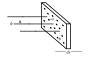
\includegraphics[width=0.8\textwidth]{images/Theory/CrossSectionSchematics.pdf}
    \caption[Cross Section Schematic View]{Shown above is a schematic view of the cross section concept. It depicts a beam of particles $a$ featuring a flux $\phi$ inciding on to a fixed target plate made of material with a width of $dx$. The cross section $\sigma$ is indicated by small areas around every target particle $b$ in the plate.}
    \label{fig:CrossSectionSchematics}
\end{figure}

\subsection{Calculating Cross Sections} \label{sec:CrossSectionCalculation}
In order to calculate cross sections from theoretical models, one first needs to derive Fermi's golden rule, introduced by P. Dirac \cite{GoldenRuleDirac} and named by E. Fermi as it became famous in his lecture on nuclear physics \cite{FermiLecture}. Hereby we will follow a similar strategy as in \cite{ModernParticlePhysics}. We start with the Schr\"odinger equation with a perturbative Hamiltonian $H = H_0 + H_{\text{int}}$, \ie
\begin{equation} \label{eq:PerturbativeSchroedinger}
    i\frac{d}{dt}\ket{\psi(t,\vec{x})} = \left( H_0 + H_{\text{int}} \right) \ket{\psi(t,\vec{x})},
\end{equation}
and then write down $\psi$ as a superposition of the eigenstates of the unperturbed Hamiltonian $\phi_n(t,\vec{x})$ given as
\begin{equation}
    \ket{\psi(t,\vec{x})} = \sum_n c_n(t) e^{-iE_nt} \ket{\phi_n(\vec{x})}.
\end{equation}
With this, we extracted the time dependent part of $\phi_n$ using the exponential term with $E_n$ being the eigenvalue of the $H_0$ operator, \ie $E_n\ket{\phi_n} = H_0\ket{\phi_n}$. If we plug above expression into our Schr\"odinger equation \ref{eq:PerturbativeSchroedinger} we end up with
\begin{equation}
    i\sum_n e^{-iE_nt} \frac{dc_n(t)}{dt} \ket{\phi_n} = \sum_n c_n(t) e^{-iE_nt} H_{\text{int}} \ket{\phi_n}. 
\end{equation}
Now it is beneficial to introduce some boundary conditions for this problem. At $t=0$ we want $\psi$ to be equal to the initial state $\phi_i$, wherefore $c_n(0)=\delta_{ni}$ is a Kronecker delta. We can further assume that the perturbation through $H_{\text{int}}$ is small enough that this still holds true for $t>0$, \ie $c_n(t) \approx \delta_{ni}$. Hence, we write the first order perturbative relation as
\begin{equation}
    i\sum_n e^{-iE_nt} \frac{dc_n(t)}{dt} \ket{\phi_n} = e^{-iE_it} H_{\text{int}} \ket{\phi_i}.
\end{equation}
Since we are interested in an amplitude of a process with an initial state $\ket{\phi_i}$ and a final state $\bra{\phi_f}$ it is appropriate to multiply $\bra{\phi_f}e^{iE_ft}$ to both sides of the equation. As different eigenstates of $H_0$ are perpendicular to one another, \ie $\braket{\phi_a|\phi_b} = \delta_{ab}$, only the $\phi_f$ terms in the sum of the left side remain non-zero. Thus, we end up with
\begin{equation}
    i\frac{dc_f(t)}{dt} = \braket{\phi_f|H_{\text{int}}|\phi_i} e^{-it(E_i-E_f)}
\end{equation}
We already encountered a term of the form like $\braket{\phi_f|H_{\text{int}}|\phi_i}$ in section \ref{sec:InitialAndFinalStates} equation \ref{eq:MatrixElement}; it is akin to a matrix element of an interaction with initial state $\phi_i$ and a final state $\phi_f$. Although in this case here it is not Lorentz invariant, for we derived it via the Schr\"odinger equation, and we name it $\widetilde{T}_{if}=\braket{\phi_f|H_{\text{int}}|\phi_i}$. Next we solve above equation for $c_f$ assuming $H_{\text{int}}$ is constant in the relevant time frame,
\begin{equation}
    c_f(t) = -i\widetilde{T}_{if} \int_{-T}^{T} dt \ e^{-it(E_i-E_f)}.
\end{equation}
Now, $c_f$ constitutes the amplitude of a process where an initial state $\phi_i$ transforms into a final state $\phi_f$. Hence, we can derive the probability of said process to occur by simply squaring the amplitude:
\begin{equation}
    P(i\to f) = \left| c_f(t) \right|^2 = \big| \widetilde{T}_{if} \big|^2 \int_{-T}^{T} dt \int_{-T}^{T} dt^{\prime} \ e^{-it(E_i-E_f)} e^{it^{\prime}(E_i-E_f)},
\end{equation}
where the integral over $dt^{\prime}$ can be solved resulting in a delta distribution term \mbox{$2\pi \delta(E_i-E_f)$}. Furthermore, we are interested in the event rate $\Gamma_{if}$, which is introduced through the relation
\begin{equation}
    d\Gamma_{if} = \frac{P_{if}}{2T} dN_{E_f} =  2\pi \big| \widetilde{T}_{if} \big|^2 \frac{1}{2T} dN_{E_f} \int_{-T}^{T} dt \ e^{-it(E_i-E_f)} \delta(E_i-E_f).
\end{equation}
Here $dN_{E_f}$ is the number of states in phase space available to the final state particle \cite{Perkins, ModernParticlePhysics}. For now we will drop the subscript of $dN$ and continue with
\begin{align}
    \Gamma_{if} &= 2\pi \int \frac{dN}{dE_f}dE_f \ \big| \widetilde{T}_{if} \big|^2 \delta(E_i-E_f) \frac{1}{2T} \int_{-T}^{T} dt \ e^{-it(E_i-E_f)}\nonumber \\
    &= 2\pi \big| \widetilde{T}_{if} \big|^2 \left. \frac{dN}{dE_f} \right|_{E_i} \frac{1}{2T} \int_{-T}^{T} dt \\
    &= 2\pi \big| \widetilde{T}_{if} \big|^2 \left. \frac{dN}{dE_f} \right|_{E_i}. \nonumber
\end{align}
With this we derived Fermi's golden rule, which is also often written with the so-called density of states $dN/dE_f|_{E_i} = \rho(E_i)$. But for our purposes we need to go back to an intermediate step of the golden rule:
\begin{equation} \label{eq:FermiGoldenRule}
    \Gamma_{if} = 2\pi \int dN \ \big| \widetilde{T}_{if} \big|^2 \delta(E_i-E_f).
\end{equation}

As an example, let us consider an interaction between two initial states $a$ and $b$ transitioning into two final states $1$ and $2$, \ie $a + b \to 1 + 2$, as in our previous example for our Feynman diagram in subsection \ref{sec:InitialAndFinalStates}. This means that we need to adjust our transition matrix element with
\begin{equation}
    \widetilde{T}_{if} = \braket{\phi_1\phi_2|\hat{H}_{\text{int}}|\phi_a\phi_b}.
\end{equation}
Furthermore, we also need to extend the delta distribution of equation \ref{eq:FermiGoldenRule} to our four states, \ie $\delta(E_i-E_f) \to \delta(E_a+E_b-E_1-E_2)$. Also, one can show \cite{ModernParticlePhysics} that for our process with an arbitrary number $m$ of final states, $dN$ is given by
\begin{equation} \label{eq:PhaseSpaceParameter}
    dN = \frac{(2\pi)^3}{V}\prod_{f=1}^m\frac{d^3p_f}{(2\pi)^3} \ \delta^{(3)}\left( \vec{p}_a + \vec{p}_b - \sum_{f=1}^m \vec{p}_f \right),
\end{equation}
where $V/(2\pi)^3$ is the volume occupied by a single state, but we set $V=1$ for now. At this point we want our golden rule formula to become Lorentz invariant and we can achieve this by replacing our matrix element $\widetilde{T}_{if}$ by the invariant matrix element we derived in \ref{eq:MatrixElementNeutrino}. For this we need to look at behaviour of the eigenstates $\phi$ after a Lorentz transformation $\phi^{\prime}$. The only difference lies in the normalisation, since
\begin{equation}
    \braket{\phi|\phi} = 1  \quad \longrightarrow \quad \braket{\phi^{\prime}|\phi^{\prime}} = 2E,
\end{equation}
Thus, we have to normalise the same way we did with the ladder operators in equation \ref{eq:aOperators} and get
\begin{equation}
    \phi^{\prime} = \frac{1}{\sqrt{2E}}\phi
\end{equation}
This implies that we are able to relate the invariant matrix element $\mathcal{M}$ with its non-invariant cousin $\widetilde{T}_{if}$ in the following manner:
\begin{equation} \label{eq:MatrixElementRelation}
    \widetilde{T}_{if} = \frac{\mathcal{M}(a+b\to 1+2)}{4\sqrt{E_a E_b E_1 E_2}}.
\end{equation}
Finally, we end up with the event rate of our process by plugging in the phase space parameter of \ref{eq:PhaseSpaceParameter}, and the invariant matrix element from \ref{eq:MatrixElementRelation} into our golden rule \ref{eq:FermiGoldenRule} and get
\begin{equation} \label{eq:EventRateCrossSection}
    \Gamma_{if} = \frac{1}{64\pi^2E_a E_b} \int \frac{d^3p_1}{E_1} \frac{d^3p_2}{E_2} \left|\mathcal{M}(a+b\to 1+2)\right|^2 \delta^{(4)}(p_a+p_b-p_1-p_2)
\end{equation}
Actually, by using the invariant matrix element, the whole equation became Lorentz invariant, since $dp^{\prime}/E^{\prime} = dp/E$.

At this point we are ready to calculate a cross section. As a matter of fact, we already discussed the missing step in the cross section introduction with equation \ref{eq:TotalCrossSectionDef}. We further know how the flux $\phi$ is defined from \ref{eq:Flux}. Thus, it is useful to combine these two equations to
\begin{equation}
    \sigma = \frac{\Gamma}{N_T n_a v_i}
\end{equation}
There is one difference though: in an experiment we need a lot of statistics, thus detectors usually feature high density targets in combination with high luminosity beams. When calculating a cross section theoretically it can be done by considering just one incident and one target particle. Hence, we set $\Gamma\to \Gamma_{if}$, $N_T = 1$, and $n_a = N_a/V = 1/V$. Remember when we set the volume $V = 1$ while calculating the phase space parameter $dN$? It is here, where the volumes cancel out when plugging in $\Gamma_{if}$ derived in equation \ref{eq:EventRateCrossSection}. Therefore, we also set $V = 1$ in this case. As a last step, it is useful to define the incident velocity as the sum of both initial particle's velocity $v_i = v_a + v_b$. With all this we end up with the formula for the cross sections for two initial particles,
\begin{equation}
    \sigma = \frac{\Gamma_{if}}{v_a + v_b}.
\end{equation}
Now we substitute $\Gamma_{if}$ and write the Lorentz invariant cross section as
\begin{equation}
    \sigma = \frac{1}{64\pi^2E_aE_b(v_a+v_b)} \int \frac{d^3p_1}{E_1} \frac{d^3p_2}{E_2} \left|\mathcal{M}\right|^2 \delta^{(4)}(p_a+p_b-p_1-p_2)
\end{equation}
In order to simplify the kinematic part, let us no longer consider an incident and a target particle, but rather look at them in the \gls{cms}. In our example the \gls{cms} implies that the sum of the incoming momenta is zero, whereby, due to momentum conservation, the same is true for the outgoing momenta. In consequence we get $\vec{p}_a = -\vec{p}_b$, and $\vec{p}_1 = - \vec{p}_2$. Let us also introduce the \gls{cms} energy $E_{\text{cms}} \coloneqq E_a + E_b$. Now we can split up the $\delta$-distribution into an energy and a momentum dependent part and integrate
\begin{align}
    \sigma &= \frac{1}{64\pi^2E_aE_b(v_a+v_b)} \int \frac{d^3p_1}{E_1} \frac{d^3p_2}{E_2} \left|\mathcal{M}\right|^2 \delta(E_{\text{cms}}-E_1-E_2) \delta^{(3)}(\vec{p}_1+\vec{p}_2) \nonumber \\
    & = \frac{1}{64\pi^2E_aE_b(v_a+v_b)} \int \frac{d^3p_1}{E_1} \frac{1}{E_2} \left|\mathcal{M}\right|^2 \delta\left( E_{\text{cms}}-\sqrt{m_1^2+\vec{p}_1^{\,2}}-\sqrt{m_2^2+\vec{p}_1^{\,2}}\right) \nonumber \\
    & = \frac{1}{64\pi^2E_aE_b(v_a+v_b)} \int d\Omega \ d|\vec{p}_1| \ \vec{p}_1^{\,2} \left|\mathcal{M}\right|^2 \frac{\delta\left( E_{\text{cms}}-\sqrt{m_1^2+\vec{p}_1^{\,2}}-\sqrt{m_2^2+\vec{p}_1^{\,2}}\right)}{\sqrt{m_1^2+\vec{p}_1^{\,2}}\sqrt{m_2^2+\vec{p}_1^{\,2}}}
\end{align}
For the last integral we parameterised for spherical coordinates, but in order to integrate we need to substitute the integration variable $|\vec{p}_1|$ with
\begin{align}
    u \coloneqq& \ \sqrt{m_1^2+\vec{p}_1^{\,2}} + \sqrt{m_2^2+\vec{p}_1^{\,2}} \nonumber \\
    \Longrightarrow \frac{du}{d|\vec{p}_1|} =& \ \frac{|\vec{p}_1| \left( \sqrt{m_1^2+\vec{p}_1^{\,2}} + \sqrt{m_2^2+\vec{p}_1^{\,2}} \right)}{\sqrt{m_1^2+\vec{p}_1^{\,2}}\sqrt{m_2^2+\vec{p}_1^{\,2}}}
\end{align}
Further, it is useful to introduce $\vec{p}_i \coloneqq \vec{p}_a = -\vec{p}_b$ and $\vec{p}_f \coloneqq \vec{p}_1 = -\vec{p}_2$. In the form factor we find the relation $E_aE_b(v_a+v_b) = E_{\text{cms}}|\vec{p}_i| = \smash{[(\vec{p}_{i\mu} \vec{p}_i^{\,\mu})^2 - m_a^2m_b^2]^{1/2}}$, where the last expression shows the Lorentz invariance of the form factor as it contains invariant four vectors. Thus, our integral takes the form
\begin{align} \label{eq:TotalCrossSectionTheory}
    \sigma &= \frac{1}{64\pi^2E_{\text{cms}}|\vec{p}_i|} \int d\Omega \ du \ \frac{|\vec{p}_f|}{u} \left|\mathcal{M}\right|^2 \delta(E_{\text{cms}}-u) \nonumber \\
    &= \frac{1}{64\pi^2E_{\text{cms}}^2} \frac{|\vec{p}_f|}{|\vec{p}_i|} \int d\Omega \left|\mathcal{M}\right|^2,
\end{align}
and the differential cross section is given by
\begin{equation} \label{eq:DiffCrossSectionTheory}
    \frac{d\sigma}{d\Omega} = \frac{1}{64\pi^2E_{\text{cms}}^2} \frac{|\vec{p}_f|}{|\vec{p}_i|} \left|\mathcal{M}\right|^2.
\end{equation}
There is one more simplification one can apply to the equation above. In the limit where the particle masses can be neglected, the centre of mass frame differential cross section is given by,
\begin{equation} \label{eq:DiffCrossSectionTheoryMassless}
    \frac{d\sigma}{d\Omega} = \frac{1}{64\pi^2E_{\text{cms}}^2} \langle \left|\mathcal{M}\right|^2 \rangle,
\end{equation}
where $\langle \left|\mathcal{M}\right|^2 \rangle$ represents the spin-averaged invariant matrix element squared \cite{ModernParticlePhysics}. More-over, by neglecting particle mass in the \gls{cms} we get $E_a = E_b$. 

So far, all the equations within this section are universally valid for any two-body to two-body interaction (with the exception of the particle mass constraints introduced in the last step). Now it is time to focus again on the main topic of this thesis: the neutrino \gls{cc} cross section. For this reason we go back to the invariant matrix element of the charged current neutrino interaction of equation \ref{eq:MatrixElementNeutrino}. When properly calculating said equation and averaging over the possible spin states of the quarks, we get
\begin{equation}
    \langle \left|\mathcal{M}\right|^2 \rangle = \frac{1}{2} \left( \frac{g_\text{w}^2}{m_W^2} E_{\text{cms}}^2 \right)^2.
\end{equation}
As can be seen, when dealing with small masses, neither the differential cross section nor the spin averaged invariant matrix element exhibit any angle dependency in the centre of mass system. Hence, the integral to calculate the total cross section from equation \ref{eq:DiffCrossSectionTheoryMassless} becomes trivial. By using the Fermi constant as defined in equation \ref{eq:FermiConstant} we get a total cross section of \cite{ModernParticlePhysics}
\begin{equation}
    \sigma(\nu_{\ell}+d \to \ell+u) = \frac{G_\text{F}^2}{\pi} E_\text{cms}^2  \approx \num{1.7e-38} \cdot E_\text{cms}^2 \ \si{\centi\metre\squared}.
\end{equation}
In the second part of above equation, $E_\text{cms}$ has to be given in \si{\giga\electronvolt}. What catches the eye is how small neutrino interaction cross sections are. With typical $E_\text{cms} = \SI{1}{\giga\electronvolt}$, the cross section only amounts to the order of \SI{e-38}{\centi\metre\squared}. This makes neutrino interactions a rare occurrence and their detection challenging. Again, note that this formula only holds true if the particle masses are irrelevant compared to the centre of mass energy, \ie $E_\text{cms} \gg \sum m_i $. Hence, it is best suited to describe electron neutrino, $\nu_e$, interactions. Moreover, due to the assumptions made to derive the invariant matrix element in equation \ref{eq:MatrixElementNeutrino}, it is required that the transferred momentum of the interaction is much smaller than the mass of the $W$-\gls{Boson}, more precisely: $q^2 \ll m_W^2$.

\subsection{Nuclear Effects}
At this point we derived a model for the cross section of a \gls{cc} neutrino interaction with a free down quark. The question now is, how to measure the cross section and verify said model, as there are no free quarks found in nature. The only reasonably stable quark carriers are the two nucleons: the proton $p$ and the neutron $n$, if the latter is bound in an atomic nucleus. Since the cross section is expected to be tiny, we require a high target density in our detector medium in order to achieve an adequate event rate. Hence, high density materials featuring many nucleons are used in modern detectors, \eg argon, the target material of MicroBooNE, features \num{40} nucleons. 

The ultimate goal of every particle physics experiment is to reconstruct all kinematic parameters of the initial particles and the interaction products. In this context, neutrino experiments face a critical difficulty for neutrino beams are not monochromatic, \ie they feature a broad energy spectrum as shown in figure \ref{fig:CrossSectionAndFlux}. Hence, the initial neutrino energy has to be reconstructed from the direct interaction products. Most detectors today are only able to measure the ionisation energy deposited by free or quasi-free charged particles with at best a millimetre spacial resolution (see chapter \ref{sec:LArTPC}). Thus, many of the observed particle traces do not originate directly form the primary interaction vertex but from daughter particles, and even daughters of daughters. For these reasons, neutrino experiments rely heavily on nuclear models for the kinematic reconstruction of the neutrino interaction.
\begin{figure}[htbp]
    \centering
    \includegraphics[width=0.7\textwidth]{images/Theory/CrossSectionGraph.pdf}
    \caption[Beam Fluxes and Neutrino Cross Section Models]{Above figure shows the neutrino flux as a function of neutrino energy for various experiments overlayed by netrino cross section models. The figure is sourced from \cite{ProgressInNuMeasurements}.}
    \label{fig:CrossSectionAndFlux}
\end{figure}

Unfortunately, the \gls{sm} is of little use to model nuclear interactions. The reason for this is the nature of the coupling constant of the strong force, $\alpha_\text{s}$, as it increases with decreasing transferred momentum. For quarks and gluons in a stable bound state like a nucleon, the coupling constant is greater than one, $\alpha_\text{s} > 1$. As established in section \ref{sec:FeynmanGraphs}, the invariant matrix element $\mathcal{M}$ is in fact a power series of Feynman diagrams of different orders and with it also a power series of $\alpha_\text{s}$. Under these circumstances it is not hard to see that that $\mathcal{M} \to \infty$ when $\alpha_\text{s} > 1$. This infinity problem is also called \textbf{running coupling} and can not be solved by renormalisation. In order to still provide a model, theorists resort to so-called \textbf{effective field theories}. These often treat nucleons and \glspl{Meson} as elementary particles, omitting their internal structure. These models are mostly limited to a certain range in transferred momentum and are subject to large systematic uncertainties. In the following paragraphs the most popular models are introduced, relying heavily on the descriptions given by M. Nirkko in his thesis \cite{PhDMartti}.

At neutrino energies in the sub-\si{\giga\electronvolt} range, $q^2$ is too low to break the target nucleus and the neutrino will scatter (quasi-)elastically. In the case of \gls{nc} interactions, neutrinos $\nu_\ell$ can scatter off nucleons $N$ elastically (neutral current elastic scattering, see figure \ref{fig:NCEL}):
\begin{equation}
    \nu_\ell + N \to \nu_\ell + N.
\end{equation}
Here, $\ell$ stands for any of the three lepton flavours. In the low energy range ($E_\nu \lesssim \SI{1}{\giga\electronvolt}$) where the neutrino energy is large enough to produce a charged lepton, but $q^2$ exchanged by the weak \gls{Boson} is not sufficient to break the target nucleus, \gls{ccqe} scattering \cite{NuQuasiElasticScattering} on neutrons (figure \ref{fig:CCQE}) is the dominant process:
\begin{equation}
    \nu_\ell + n \to \ell^- + p.
\end{equation}
These interactions are important to neutrino physics for a number of reasons. Most notably, their nature as two-body interactions enable the kinematics to be fully reconstructed: Assuming an initial nucleon at rest, the neutrino energy can be inferred:
\begin{equation}
    E_\nu = \frac{m_n E_\ell + \frac{1}{2}(m_p^2 + m_n^2 + m_\ell^2)}{m_n - E_\ell + p_\ell \cos{(\theta_\ell)}},
\end{equation}
where $m_x$ is the mass of the nucleons ($n$ or $p$) or the produced lepton $\ell$. Moreover, $p_\ell$ and $E_\ell$ are the lepton momentum and energy, respectively. Finally, $\theta_\ell$ denotes the scattering angle with respect to the incident neutrino momentum. However, above formula becomes significantly more complicated when the nucleon is not free but bound in a large atomic nucleus like argon \cite{PhDMartti}. This theory was extended to larger nuclei with the \gls{rfg} model, which treats nucleons as quasi-free with Fermi momentum, in the mean field of the nucleus, where the nuclear parameters are tuned to electron scattering data \cite{ProgressInNuMeasurements}. However, the predictions of said model are quite poor leading to MiniBooNE's ``\gls{ccqe} puzzle'' \cite{AxialMassMiniBooNE}, when a significantly greater cross section was extracted from the data than seen in earlier experiments using deuterium, \ce{^2H}, as their target material. Evidently, the non-trivial nuclear effects at the \gls{ccqe} energy scale must not be omitted.
\begin{figure}[htbp]
    \centering
    \subfloat[Neutral Current Elastic Scattering][Neutral current elastic scattering]
    {
        \includegraphics[width=0.49\textwidth]{images/Theory/NCEL.pdf}
        \label{fig:NCEL}
    }
    \subfloat[Charged Current Quasi-Elastic Scattering][Charged current quasi-elastic scattering]
    {
        \includegraphics[width=0.49\textwidth]{images/Theory/CCQE.pdf}
        \label{fig:CCQE}
    }
    \caption[MicroBooNE TPC]{Shown above are the Feynman diagrams of the neutral current elastic scattering in \subref{fig:NCEL}, and of the charged current quasi-elastic scattering \subref{fig:CCQE}. As an example, the primary particle is chosen to be $\nu_\mu$. Sourced from \cite{PhDMartti}.}
    \label{fig:NCELandCCQE}
\end{figure}

At intermediate neutrino energies (\SIrange{1}{10}{\giga\electronvolt}), higher values of $q^2$ become available, and neutrinos can begin to scatter inelastically. While the leptonic side of the interaction does not change, on the hadronic side the nucleon can be boosted into an excited state (baryonic resonance, \eg \ch{N^*}, $\Delta$). These resonances then decay back to a nucleon in the ground state, often accompanied by a pion. However, depending on the type of resonance a variety of final states is possible, including multiple pions, kaons or a radiative photons. These interactions are known as \gls{res}, the most common result being the production of a single pion ($\num{1}\pi$). A typical resonant interaction is
\begin{equation}
    \nu_\ell + p \to \ell + \Delta^{++} \to \ell + \pi^+ + p^\prime,
\end{equation}
whith the $W$-\gls{Boson} converting the down-quark in the initial proton to an up-quark, resulting in a seemingly symmetric state ($\Delta^{++} = uuu$) which decays into a proton and a pion (figure \ref{fig:CCRES}) \cite{PhDMartti}.
\begin{figure}[htbp]
    \centering
    \includegraphics[width=0.5\textwidth]{images/Theory/CCRES.pdf}
    \caption[Charged Current Resonant Interaction]{Depicted here is the Feynman diagram for a charged current resonant interaction: A muon-neutrino interacts with a proton, causing it to reach an excited state ($\Delta^{++}$ resonance), which decays into a proton and a single pion \cite{PhDMartti}.}
    \label{fig:CCRES}
\end{figure}

At high neutrino energies ($E_\nu \gtrsim \SI{10}{\giga\electronvolt}$), values of $q^2$ can become high enough for the internal structure of the nucleon to be resolved. The neutrinos can then scatter directly off the quarks within, which is known as \gls{dis}. The process is not limited to valence quarks; scattering can also occur off ``sea quarks'' that continuously pop in and out of existence in a nucleon. A consequence of this interaction is inevitably the break up of the target nucleon: As the struck quark recoils, the nucleon fragments and the strong forces between quarks result in hadronisation, \ie the production of multiple hadrons. The final state often includes multiple pions and nucleons exiting the shattered nucleus (see figure \ref{fig:DIS}), resulting in events with high track multiplicity \cite{PhDMartti}.
\begin{figure}[htbp]
    \centering
    \includegraphics[width=0.5\textwidth]{images/Theory/DIS.pdf}
    \caption[Charged Current Deep Inelastic Scattering]{Above is a Feynman diagram for a neutrino interacting via charged current deep inelastic scattering. The nucleon $N$ is shattered, causing multiple pions $n\pi^{\pm,0}$ and other hadrons $X$ to be produced \cite{PhDMartti}.}
    \label{fig:DIS}
\end{figure}

The cross section of the three described (anti-)neutrino interaction modes as a function of neutrino energy is depicted in figure \ref{fig:CrossSectionDistribution}. It shows experimentally determined data points as well as the above-described model predictions (solid lines). As can be seen, the models do not match the data points in many cases. This state of affairs, especially the \gls{ccqe} discrepancies, prompted many particle physicists to rethink these interaction categories as a whole. This new approach will be described in the next paragraph.
\begin{figure}[htbp]
    \centering
    \subfloat[Neutrino Cross Section][Neutrino cross section]
    {
        \includegraphics[width=0.45\textwidth]{images/Theory/NuCrossSection.pdf}
        \label{fig:NuCrossSection}
    }
    \subfloat[Antineutrino Cross Section][Antineutrino cross section]
    {
        \includegraphics[width=0.45\textwidth]{images/Theory/AntiNuCrossSection.pdf}
        \label{fig:AntiNuCrossSection}
    }
    \caption[Neutrino and Antineutrino Cross Section]{Shown here are experimentally observed cross sections for \subref{fig:NuCrossSection} neutrino and \subref{fig:AntiNuCrossSection} antineutrino interactions. The models of the dominant reaction types and the total cross section are shown as solide lines as a function of energy. Sourced from \cite{PhDMartti} and influenced by \cite{CrossSectionReview}.}
    \label{fig:CrossSectionDistribution}
\end{figure}

As established before, hadrons produced within neutrino interactions can rescatter before exiting the nucleus, thereby significantly modifying the outgoing hadron composition and kinematics that are experimentally observed. Such rescattering processes are typically known as \gls{fsi}. Since it is impossible to look inside the nucleus to see what is going on (as shown schematically in figure \ref{fig:FSI}), these interactions can only be inferred by nuclear models, and by precisely measuring the final state kinematics of any observable particles leaving the nucleus \cite{PhDMartti}. This means that we are unable to reasonably measure \gls{ccqe}, instead we can observe an event topology with a single charged lepton and no pions (\gls{cc}$0\pi$). This certainly contains \gls{qe} events but neither exclusively nor completely. As we do not want to assume a model for these processes, we can only measure cross sections for a given post-\gls{fsi} signature. Mathematically these measured cross sections are defined as \cite{ProgressInNuMeasurements} 
\begin{equation}
    \tilde{\sigma}_n(\mathbf{k}) = \sum_{m} \int_{E_\text{min}}^{E_\text{max}} dE_\nu \ \sigma_m(E_\nu,\mathbf{k}^{\prime}) \text{FSI}(\mathbf{k}^{\prime},\mathbf{k}),
\end{equation}
where $E_\nu$ denotes the neutrino energy in the $E_\text{min}$ to $E_\text{max}$ range output by the neutrino beam line. $\sigma_i$ is the cross section of the true process categories, and the function $\text{FSI}(\mathbf{k^\prime},\mathbf{k})$ transforms the kinematics of the initial interaction products $\mathbf{k}^\prime$ into the kinematics of the post-\gls{fsi} particles $\mathbf{k}$. These kinematics $\mathbf{k}^{(\prime)}$ are mostly given by the momentum and the scattering angle of a particle, \eg $p_\mu^{(\prime)}$ and $\theta_\mu^{(\prime)}$. Note, not only did we change the definition of the cross section but we also changed the definition of the final state: it is now the particles as measured in the detector and not as created by the primary neutrino interaction. This change in philosophy also meant to collaborate with nuclear physicists to create the needed models \cite{NuclearModels,GIBUU}. At this point we can also better understand the main topic of this thesis, \ie the $\nu_\mu$ \gls{cc} inclusive cross section measurement. This event topology describes a \gls{cc} final state, with any hadronic final state configuration (including no hadrons), meaning that every neutrino event with a muon is counted. In view of the new nuclear models, the \gls{cc} inclusive cross section is given by the sum of all possible \gls{cc} related sub-processes, thus it can be used to tune the initial interaction model. The \glspl{fsi} do not matter in this case as we accept all of them with the inclusive event signature \cite{NuclearModels,GIBUU}.
\begin{figure}[htbp]
    \centering
    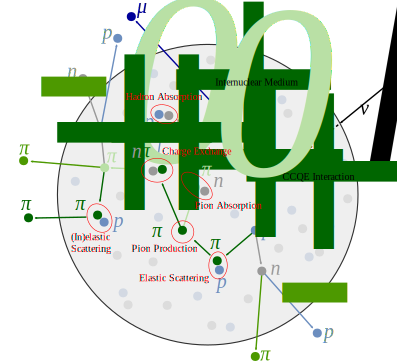
\includegraphics[width=1.0\textwidth]{images/Theory/FSI.pdf}
    \caption[Final State Interaction Example]{Illustrated here, is an example of \glspl{fsi}. First, the inciding muon neutrino $\nu_\mu$ represented by the black arrow followed by the dashed black line scatters via a \gls{ccqe} interaction with a neutron of an argon nucleus. The produced negatively charged muon (indigo) and the positively charged proton (light blue) traverse through the nuclear medium and are subject to nuclear effects (nuclear binding energy, Coulomb distortion, etc.). In the second step, the proton can undergo various types of \glspl{fsi} which may lead to even more \glspl{fsi} such as (in)elastic scattering, pion production, hadron absorption and charge exchange. The pions ($\pi^+$, $\pi^-$, and $\pi^0$) in this figure are shown in dark, lighter, and light green, respectively \cite{CrossSectionFSI}.}
    \label{fig:FSI}
\end{figure}

\subsection{Measuring Cross Sections} \label{sec:MeasuringCrossSection}
Every cross section measurement starts with a measured event rate in a detector. Said rate is dependent on the detector itself, the event reconstruction, and the event selection process. In other words, the rate may vary strongly for every analysis. To receive universally comparable results, we use \gls{mc} models to quantify the effects of this selection bias. In order to achieve this, whole events have to be simulated starting with the neutrino interaction and ending with the readout electronics response of the detector. These \gls{mc} events should now be almost indistinguishable from raw events measured with the detector. Hence, these models need to be of excellent quality. The events are then subjected to the very same reconstruction and selection algorithms as the real detector data. The \gls{mc} data sets provide vital truth information which can then be compared to the selected reconstruction events. Two often used quantities to determine the quality of a selection process are the purity $p$ and the efficiency $\epsilon$. The purity is a measure of how many of the selected events are true signal events, and the efficiency indicates how many of the true signal events were selected, \ie 
\begin{equation}
    p \coloneqq \frac{\text{\# selected signals}}{\text{\# total selected}}, \qquad \epsilon \coloneqq \frac{\text{\# selected signals}}{\text{\# total signals}}.
\end{equation}
Both variables are often used to optimise the cut values of the various selection steps. The most prominent method is to maximise the products of the two \cite{EfficiencyTimesPurity}, \ie $\max{(p\epsilon)}$, as will be shown in chapter \ref{sec:FistCCInclusive}. After selection process, the truth information allows us to distinguish between the number of selected signal events, $S$, and the number of selected background events $B$. In total both amount to the total number of selected events $N = S+B$.

The results of a cross section analysis are usually distributions in at least one kinematic parameter $k$. Said distributions are in histogram form, \ie they are binned. Consequently, the selection numbers also need to be binned and we get $N_i = S_i + B_i$. When dealing with a \gls{mc} sample, it is useful to compare the reconstructed with the true distributions. This is done with the so-called \textbf{smearing matrix} $U_{ij}$, which describes the mapping between a true bin $j$, and a reconstructed bin $i$. It is defined as
\begin{equation} \label{eq:SmearingMatrix}
    U_{ij} \coloneqq \frac{\text{\# selected reconstruction events in bin }i \text{ with a truth value in bin }j}{\text{\# generated truth events in bin }j}.
\end{equation} 
From this, the bin efficiency $\epsilon_j$ can be extracted with $\epsilon_j = \sum_i U_{ij}$. This indicates that the selection efficiency is also incorporated into the smearing matrix.

With these tools we are now able to derive the formula to calculate differential cross sections from event rates. As a matter of fact, we were already very close with the differential cross section formula of equation \ref{eq:DiffCrossSection}, although in practice one uses binned histograms, instead of a continuous function. This means that $d\sigma/dk$ is transformed to $\delta\sigma/\delta k_j$, where $\delta k_j$ is equivalent to the width of bin $j$. As is indicated by the bin index $j$, we will transform the differential cross section from reconstructed space into true space to allow for comparisons with cross section models. Therefore, the smearing matrix needs to be inverted ($U_{ij}^{-1}$), but this often leads to large fluctuations in the resulting matrix elements, as statistical uncertainty in the reconstruction space is blown up by the inversion \cite{ProgressInNuMeasurements}. Sometimes $U_{ij}$ is not even invertible, hence, the pseudoinverse $\widetilde{U}^{-1}_{ij}$, also called \textbf{unfolding matrix}, is utilised to map the reconstruction bis into true bins. Now, the formula to extract the differential cross section from detector data is given by
\begin{equation} \label{eq:CrossSectionMeasurement}
    \frac{\delta\sigma^\text{real}}{\delta k_i} = \frac{\sum_j \widetilde{U}^{-1}_{ij} \left( N_i^\text{real} - B_i \right)}{\delta k_i \Phi_{\nu} N_T}.
\end{equation}
Note, that the neutrino beam flux $\Phi_{\nu}$ as well as the number of target nucleons are constants and remain unbinned as in equation \ref{eq:DiffCrossSection}. Furthermore, it is important to stress that $N_i^\text{real}$ is the number of selected real world event in bin $i$. Depending on the detector technology, the background $B_i$ can be a combination of expected background determined from the \gls{mc} model and real world background measurements.

Now let us take a step back and have a look at the bigger picture of measuring a cross section. The goal of a cross section measurement ought to be the comparison of real world data with \gls{mc} models in order to validate or refute them. For this purpose, our data needs to model independent, otherwise we might introduce a bias. However, the unfolded cross section method discussed above does not fulfil the model independence requirements. In this case, model dependency is introduced with the smearing matrix $U_ij$ and background predictions in $B_i$, when a \gls{mc} neutrino generator is used at the beginning of the simulation process. This generator often even uses the models we use to compare the data to. How large this bias really is, has yet to be investigated \cite{ForwardFolding}. Nevertheless, it might be a good idea, to remove as much model dependence as possible from a cross section analysis. This exact philosophy led to the development of forward-folding analysis methods. The idea here is to use the raw real world data selection $N_i^\text{real}$ as is and forward-fold the \gls{mc} selection to resemble the data. In mathematical form forward-folding is described by \cite{CRTThomasPhD}
\begin{equation} \label{eq:ForwardFolding}
    N_i^\text{mc} = \Phi_\nu N_T \sum_j U_{ij} \sigma_j^\text{mc} + B_i
\end{equation}
In this case, $N_i^\text{mc}$ is the number of events in reconstructed space as predicted by the \gls{mc} simulation which will be compared to $N_i^\text{real}$. Moreover, $\sigma_j^\text{mc}$ is the \gls{mc} cross section model in true space which we want to compare our data to. With this approach, we keep the model dependencies on the \gls{mc} side of the comparison. As can be seen, forward-folding also spares us from inverting $U_{ij}$ which is proven to be statistically advantageous \cite{ForwardFolding}. However, there are also disadvantages, mostly of political nature. The first problem is already represented by the formula above. It indicates a shifts of responsibility for achieving model comparability from the experimentalist to the modellers. So far, the modellers' tools produce real cross section distributions which now need to be forward-folded. This only gets more complicated once systematic uncertainties enter the game. With this arises the next problem: people are simply not used to forward-folding, these distributions do not make sense to them. Still, in this thesis all cross section related measurements make use of the forward folding method. The results of said measurements are found in the chapters \ref{sec:FistCCInclusive} and \ref{sec:NewCCInclusive}.

\end{fmffile}


% TODO Find Place for this discription
% \section{Neutrino Properties}
% There are three experimentally confirmed neutrino flavours in the \gls{sm}: the electron neutrino $\nu_e$, the muon neutrino $\nu_\mu$, and the tau neutrino $\nu_\tau$. According to the \gls{sm} all neutrino flavours have a corresponding antiparticle which are represented by the symbols $\bar{\nu_e}$, $\bar{\nu_\mu}$, and $\bar{\nu_\tau}$. Neutrinos are spin-\textonehalf{} particles (\glspl{Fermion}) and belong to the group of leptons in the \gls{sm}. They hold neither electrical, nor color charge.  Neutrinos exhibit unique behaviour as particles. For instance, they only interact through weak interaction by exchanging on of the three gauge \glspl{Boson} $W^{\pm}$ and $Z_0$. They are also assumed to have the lowest masses of any \glspl{Fermion} in the \gls{sm}, with the most recent upper limit of $m_{\nu_e} < \SI{0.8}{\electronvolt}$ (\SI{90}{\percent} \gls{cl}) \cite{NeutrinoMass}. This leads to neutrino oscillation, which by itself is a very particular occurrence only observed in neutrinos and will be discussed later in this section. Furthermore, neutrinos seem to have a unique chirality property, \ie there are only neutrinos with left-handed chirality (see section \ref{sec:WeakInteractionTheory}).
% % TODO Mention very low cross section
% 
% % TODO Find a place for this discription
% % TODO reference to momentum and angular momentum conservation of the lagrangian
% \subsection{Parity, Charge Conjugation, and Time Reversal}
% The very backbone of particle physics is the concept of symmetry or invariance of equations under various operations such as rotations or translations in spacetime. In general, symmetries are closely linked to conservation laws. In case of rotations and translations the linked conserved properties are angular- and linear momentum respectively, as mentioned in section \ref{sec:StandardModel}. Three important discrete symmetries are parity, charge conjugation, and time reversal. They are introduced through transformation operators and often used in combination with each other. The parity transformation inverts the spacial coordinates, charge conjugation transforms a particle into its antiparticle, and time reversal inverts the time line.
% 
% As mentioned above the parity transformation causes an inversion of all spatial coordinates $(x,y,z) \to (-x,-y,-z)$. Thus we introduce an operator $\mathcal{P}$ with the following properties:
% \begin{equation}
%     \mathcal{P}\psi(t,x,y,z) = \psi(t,-x,-y,-z).
% \end{equation}
% $\mathcal{P}$ is an unitary operator and produces the eigenvalues $P = \pm1$. This can be shown with two simple example, for simplicity only in one dimension:
% \begin{align}
%     \psi(x) &= \cos(x), \nonumber \\
%     \mathcal{P}\psi(x) &= \psi(-x) = \cos(-x) = \cos(x) = \psi(x), \nonumber \\
%     \Rightarrow P &= +1. \nonumber
% \end{align}
% Thus follows, the cosine function has a parity of $+1$, also called even parity. If we do the same with the sine function we get
% \begin{align}
%     \psi(x) &= \sin(x), \nonumber \\ 
%     \mathcal{P}\psi(x) &= \psi(-x) = \sin(-x) = -\sin(x) = -\psi(x),  \nonumber \\
%     \Rightarrow P &= -1. \nonumber
% \end{align}
% So, the sine function has a parity of $-1$ or odd parity. Sometimes, if $P \neq \pm1$, parity has no defined eigenvalue, \eg
% \begin{align}
%     \psi(x) &= \cos(x) + \sin(x), \nonumber \\
%     \mathcal{P}\psi(x) &= \cos(x) - \sin(x) \neq \pm \psi. \nonumber
% \end{align}
% In this case $\mathcal{P}$ only inverts the coordinates but does create an eigenvalue $P$ infront of the wave function \cite{Perkins}. 
% 
% How is this parity operator tied to a symmetry in particle physics? To answer this question we need to consider particle interactions: if they could occur regardless of the space coordinate inversion, parity is conserved. To the best of our experimental knowledge parity is conserved in all strong and \gls{em} interactions \cite{StandardModel}. It was long believed that parity invariance poses an universal law valid for all particle interactions. In 1956, however, T.D. Lee and C.N. Yang \cite{ParityLeeYang} suspected that parity is not conserved in weak interactions, which was later confirmed by C.S. Wu \cite{ParityWu} in her famous experiment. This originates from the chirality and helicity of the neutrino and the existence of only one handedness which will be discussed in the next section (\ref{sec:ChiralityHelicity}). As R. Mann put it in his Book \cite[Nature is not mirror-symmetric - parity is violated!]{StandardModel}.
% 
% Charge conjugation transforms any state into a state with reversed charge, while energy, momentum, spin, and mass stay the same. In other words each particle $\ket{p}$ gets transformed into its anti-particle $\ket{\bar{p}}$ and vice versa. Therefore the charge conjugation operator $\mathcal{C}$ is introduced,
% \begin{equation}
%     \mathcal{C} \ket{p} = \ket{\bar{p}} \quad \text{\eg} \quad \mathcal{C} \ket{\pi^+} = \ket{\pi^-}.
% \end{equation}
% $\mathcal{C}$ is, as $\mathcal{P}$, a unitary operator and exhibits also the eigenvalues $C = \pm 1$. However, unlike parity, most particles are not eigenstates of $\mathcal{C}$ because a particle is not the same eigenstate as its antiparticle ($\ket{\nu} \neq \pm\ket{\bar{\nu}}$). Hence, $\mathcal{C}$ only produces eigenvalues on particle eigenstates that are their own antiparticle, because eigenvalue equation for $\mathcal{C}$ requires
% \begin{equation}
%     \mathcal{C} \ket{p} = \ket{\bar{p}} = \pm \ket{p}.
% \end{equation}
% Only a hand full of particles, all of the \glspl{Boson}, meet said requirement: $\gamma$, $\pi^0$, $\eta$, $\eta^{\prime}$, $\rho$, $\phi$, and $J/\psi$ \cite{StandardModel}.
% 
% The charge conjugation symmetry by itself is adhered to in \gls{em} and strong interactions. However, it is not a symmetry of all weak interactions since $\mathcal{C}$ applied to a left-handed neutrino, would result in a left-handed anti-neutrino \ie a neutrino with opposite weak charge. Therein lies the same problem as with parity, left-handed anti-neutrinos are not observed in nature \cite{StandardModel}. What would happen if we combined the two symmetries, \eg
% \begin{equation} \label{eq:NuCPViolation}
%     \mathcal{CP} \ket{\nu} = \ket{\bar{\nu}}.
% \end{equation}
% Here, $\mathcal{P}$ transforms a left-handed neutrino into a right-handed one. Thereafter $\mathcal{C}$ transforms the right-handed neutrino into a right-handed antineutrino. This seems to work, but there is a catch: a general CP-symmetry in all particle physics processes would imply a perfect balance of matter and antimatter in the universe which in itself is a contradiction to humanity's very existence. In this sense unsurprisingly, CP-violation was first found in the decay of neutral kaons $K^0$ and $\bar{K}^0$, notably again a week interaction \cite{CP-Violation}. The measured asymmetry, is so small (of the order of \num{1e-3}) that one could state: $\mathcal{CP}$ is almost conserved. So far CP-violation is only mesured in baryon decays. In the lepton sector CP-violation is expected to be the tied via a see-saw mechanism with the baryon sector \cite{NeutrinoCPViolation}. Therefore above equation \ref{eq:NuCPViolation} is invalid by a small fraction. Neutrino models include CP-violation (see neutrino mixing in section \ref{sec:MixingOscillation}), although measuring it is deemed very challenging. 
% % TODO Check the order of cp violation 10^-3 or even smaller
% 
% Time reversal transformation causes an inversion of the time component of a wave function, \ie $t \to -t$, and is introduced through time reversal operator $\mathcal{T}$:
% \begin{equation}
%     \mathcal{T}\psi(t,x,y,z) = \psi(-t,x,y,z).
% \end{equation}
% With time, the operator also inverts all momenta as well as spin. It is probably the most abstract of the three introduced symmetries, as the ever expanding universe or the second law of thermodynamics and its associated concept of ever increasing entropy affirm the existence of irreversible processes in physics. They are clear indicators of the unidirectionality of time and thus a universal time reversal symmetry can not exist on a macroscopic level; for example while reversing time the universe would not expand anymore as it does now, but rather contract. At the microscopic level, which particle physics is definitely a part of, the situation is quite different and there are time reversible processes like the scattering of a neutron $n$ and a proton $p$ to produce deuteron $D$  and a photon $\gamma$:
% \begin{equation}
%     n + p \rightarrow D + \gamma \Leftarrow \mathcal{T} \Rightarrow D + \gamma  \rightarrow n + p. \nonumber
% \end{equation}
% In this case the rate of both processes is the same for corresponding conditions of energy and momenta and they are therefore T-invariant. Moreover, all experiments seem to confirm time reversal symmetry for strong and \gls{em} interactions. Unfortunately it is hard to measure T-invariance in weak interactions and thus far experiments have not produced any results, so we can not discuss the implication of time reversal for neutrinos (which makes me a sad panda).
% 
% Nevertheless, we can again take a look at a combination of symmetries. So let us consider the combination of all three, \ie the CPT-Symmetry first introduced by J. Schwinger \cite{CPT-Invariance}. It is deemed to be one of the fundamental laws of particle physics that CPT-invariance holds for all particle interactions. This law is called the CPT theorem and can be derived using assumptions of Lorentz invariance, quantum field theory. Therefore, if CPT-violation were detected quantum field theory would crumble down as a valid description of nature and would hint at beyond standard model physics. CPT-invariance has several implications:
% \begin{enumerate}
%     \item A Particle and its antiparticle must have the same mass
%     \item A Particle and its antiparticle must have the same lifetimes
%     \item A Particle and its antiparticle must have the same magnetic moments
% \end{enumerate}
% So far, measuring these quantities for several particles and their antiparticles resulted in confirmation of CPT-invariance. Since CPT theorem seems to hold true and CP-violation is detected in weak interactions , logic dictates, that weak interaction must violate the T-symmetry too \cite{Perkins,Griffiths,StandardModel}.
% 
% % TODO Find a place for this discription
% \subsection{Chirality and Helicity} \label{sec:ChiralityHelicity}
% After the discovery of parity violation in weak interactions two concepts became ubiquitous in particle physics: helicity and chirality, both describing the spin rotation properties of particles. The helicity operator is simply defined as the projection of spin $\vec{S}$ of a particle onto its three momentum $\vec{p}$:
% \begin{equation}
%     \mathpzc{h} \coloneqq 2\frac{\vec{S}\cdot\vec{p}}{\left| \vec{p} \right|},
% \end{equation}
% where the factor 2 is used to follow normalisation conventions for spin-\textonehalf{} particles. The operator $\mathpzc{h}$ produces the eigenvalues of $h = +1$ for right-handed, and $h = -1$ for left-handed particles. Figure \ref{fig:NeutrinoHelicity} visualises above equation in a less abstract manner. Chirality, on the other hand, is an intrinsic property of a particle depending on the four-momentum $p$ incorporated in the Dirac spinors $u(p)$ and $v(p)$. These chiral Dirac spinors are discussed in sections \ref{sec:DiracSpinors} as well as \ref{sec:WeakInteractionTheory} and are listed in table \ref{tab:ChiralSpinors}. While the handedness definition of helicity is the same for particles and antiparticles, the sign flips in case of chirality.
% \begin{figure}[htbp]
%     \centering
%     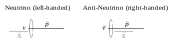
\includegraphics[width=1.0\textwidth]{images/Theory/NeutrinoHelicity.pdf}
%     \caption[Helicity of Neutrinos and Anit-Neutrinos]{The helicity states of neutrinos and anti-neutrinos are depicted here, while $\vec{p}$ indicates the momentum and $\vec{S}$ the spin of the particle. For neutrinos the spin is always anti-parallel to the momentum, while for anti-neutrinos they are both parallel. Looking at above picture it becomes obvious why a space coordinate inversion would fail and thus why parity is violated.}
%     \label{fig:NeutrinoHelicity}
% \end{figure}
% For massless particles chirality and helicity are equal and opposite for massless antiparticles. So if a massless left-handed neutrino created, it will exhibit the same helicity for all observers regardless of their inertial reference frame. But for massive particles helicity is not a Lorentz-invariant quantity. Thus an observer could overtake a massive neutrino in flight, which would change the direction of $\vec{p}$ by \SI{180}{\degree} leaving the spin unchanged. Said observer would therefore see the prohibited state of a right-handed neutrino. Hence neutrinos were long belived to be massles yet in 1998 the Super-Kamiokande observed neutrino oscillation \cite{NuOscillationDiscovery} and thus demonstrated that ther is a mass difference between neutrinos (will be properly discussed section \ref{sec:MixingOscillation}). Today it is established that there are three neutrinos all differing in mass wherefore at least two of those masses must be non-zero. For this reason one could imagine an experiment where the target particle would catch up with a neutrino from behind. With this direct persuit method one could measure the helicity reversal and the absolute mass of a neutrino as well, though it would be extremly hard to produce such an experiment. First it would requires very high energy electron beams in the order of \SI{10}{\tera\electronvolt} and second both, neutrino and electron beams would require extremely high luminosity, due to the low cross section of neutrino interactions \cite{NeutrinoHelicityChirality}. Nevertheless there is a feasable to perform the measurement through neutrinoless double beta decay, which we will explore in the next section. 
% 
% \subsection{Dirac - or Majorana Fermion} \label{sec:DiracOrMajorana}
% There is a way out of the contradiction that there are only left-handed neutrinos (right-handed antineutrinos) and that neutrinos have non-zero mass. In 1937 Ettore Majorana hypotesised a fermion that is its own anitparticle \cite{MajoranaFermionTheory}. So far there are only a fiew \glspl{Boson} with this property and we alredy explored them while discussing charge conjugation above.
% 
% \begin{figure}[htbp]
%     \centering
%     \subfloat[Double-Beta Decay][Double-Beta Decay]
%     {
%     \begin{fmffile}{feynman/DoubleBeta}
%     \fmfset{arrow_len}{2.5mm} % smaller arrows, default 4mm
%     \fmfset{zigzag_width}{1thick}
%     \fmfset{dash_len}{1.5mm}
%         \fmfframe(30,30)(30,30){
%         \begin{fmfgraph*}(120,120)
%             \fmfstraight
%             \fmfleft{i1,i2,i3,i4}
%             \fmfright{o1,o2,o3,o4,o5,o6}
%             % lower fermions
%             \fmfv{label=$\bar{\nu}_e$,label.angle=-20,label.dist=1mm}{o2}
%             \fmfv{label=$e^-$,label.angle=20,label.dist=1mm}{o3}
%             \fmf{fermion,tension=1}{o2,v2,o3}
%             % upper fermions
%             \fmfv{label=$\bar{\nu}_e$,label.angle=-20,label.dist=1mm}{o4}
%             \fmfv{label=$e^-$,label.angle=20,label.dist=1mm}{o5}
%             \fmf{fermion,tension=1}{o4,v3,o5}
%             % Phantoms
%             \fmf{phantom}{i1,v2,v3,i4}
%             \fmf{phantom,tension=2}{i1,v1} % to help \quark
%             \fmf{phantom,tension=2}{i4,v4} % to help \quark
%             \fmf{phantom}{v1,o1} % to help \quark
%             \fmf{phantom}{v4,o6} % to help \quark
%             % virtices
%             \fmfv{decor.shape=circle,decor.filled=full,decor.size=1thick}{v2}
%             \fmfv{decor.shape=circle,decor.filled=full,decor.size=1thick}{v3}
%             \fmffreeze
%             % bosons
%             \fmf{zigzag,label=$W^{-}$,label.side=left,label.dist=1mm}{v1,v2} % lower
%             \fmf{zigzag,label=$W^{-}$,label.side=right,label.dist=1mm}{v4,v3} % upper
%             % lower quarks
%             \fmfv{l=$n$\mylbrace{30}{-7}{2},l.d=16,l.a=-160}{i1}
%             \fmfv{l=\myrbrace{30}{-7}{2}$p$,l.d=16,l.a=-20}{o1}
%             \quark{qldi}{$d$}{0,1}{1.00,1}{0,  0}{left} {0, 0}{0,0}{i1,v1}
%             \quark{qlei}{$d$}{0,1}{1.00,1}{0, -9}{left} {0, 0}{0,0}{i1,v1}
%             \quark{qlfi}{$u$}{0,1}{1.00,1}{0,-18}{left} {0, 0}{0,0}{i1,v1}
%             \quark{qldo}{$u$}{0,1}{1.00,1}{0,  0}{right}{0, 0}{0,0}{v1,o1}
%             \quark{qleo}{$d$}{0,1}{1.00,1}{0, -9}{right}{0, 0}{0,0}{v1,o1}
%             \quark{qlfo}{$u$}{0,1}{1.00,1}{0,-18}{right}{0, 0}{0,0}{v1,o1}
%             % upper quarks
%             \fmfv{l=$n$\mylbrace{30}{28}{2},l.d=16,l.a=-160}{i4}
%             \fmfv{l=\myrbrace{30}{28}{2}$p$,l.d=16,l.a=-20}{o6}
%             \quark{qudi}{$d$}{0,1}{1.00,1}{0,  0}{left} {0, 0}{0,0}{i4,v4}
%             \quark{quei}{$d$}{0,1}{1.00,1}{0, +9}{left} {0, 0}{0,0}{i4,v4}
%             \quark{qufi}{$u$}{0,1}{1.00,1}{0,+18}{left} {0, 0}{0,0}{i4,v4}
%             \quark{qudo}{$u$}{0,1}{1.00,1}{0,  0}{right}{0, 0}{0,0}{v4,o6}
%             \quark{queo}{$d$}{0,1}{1.00,1}{0, +9}{right}{0, 0}{0,0}{v4,o6}
%             \quark{qufo}{$u$}{0,1}{1.00,1}{0,+18}{right}{0, 0}{0,0}{v4,o6}
%         \end{fmfgraph*}
%         }
%         \end{fmffile}
%         \label{fig:FeynmanDoubleBetaDecay}
%     }
%     \subfloat[Neutrinoless Double-Beta Decay][Neutrinoless Double-Beta Decay]
%     {
%     \begin{fmffile}{feynman/NulessDoubleBeta}
%     \fmfset{arrow_len}{2.5mm} % smaller arrows, default 4mm
%     \fmfset{zigzag_width}{1thick}
%     \fmfset{dash_len}{1.5mm}
%         \fmfframe(30,30)(30,30){
%         \begin{fmfgraph*}(120,120)
%             \fmfstraight
%             \fmfleft{i1,i2,i3,i4}
%             \fmfright{o1,o2,o3,o4}
%             % lower fermions
%             \fmfv{label=$e^-$,label.angle=0,label.dist=1mm}{o2}
%             \fmf{fermion,tension=2}{v2,o2}
%             % upper fermions
%             \fmfv{label=$e^-$,label.angle=0,label.dist=1mm}{o3}
%             \fmf{fermion,tension=2}{v3,o3}
%             % phantoms
%             \fmf{phantom}{i1,v2,v3,i4}
%             \fmf{phantom,tension=2}{i1,v1} % to help \quark
%             \fmf{phantom,tension=2}{i4,v4} % to help \quark
%             \fmf{phantom}{v1,o1} % to help \quark
%             \fmf{phantom}{v4,o4} % to help \quark
%             \fmffreeze
%             % bosons
%             \fmf{zigzag,label=$W^{-}$,label.side=left,label.dist=1mm}{v1,v2} % lower
%             \fmf{zigzag,label=$W^{-}$,label.side=right,label.dist=1mm}{v4,v3} % upper
%             % neutrino
%             \fmf{plain,label=$\nu_{e}$,label.side=right,label.dist=1mm}{v2,v3}
%             % virtices
%             \fmfv{decor.shape=circle,decor.filled=full,decor.size=1thick}{v2}
%             \fmfv{decor.shape=circle,decor.filled=full,decor.size=1thick}{v3}
%             % lower quarks
%             \fmfv{l=$n$\mylbrace{30}{-7}{2},l.d=16,l.a=-160}{i1}
%             \fmfv{l=\myrbrace{30}{-7}{2}$p$,l.d=16,l.a=-20}{o1}
%             \quark{qldi}{$d$}{0,1}{1.00,1}{0,  0}{left} {0, 0}{0,0}{i1,v1}
%             \quark{qlei}{$d$}{0,1}{1.00,1}{0, -9}{left} {0, 0}{0,0}{i1,v1}
%             \quark{qlfi}{$u$}{0,1}{1.00,1}{0,-18}{left} {0, 0}{0,0}{i1,v1}
%             \quark{qldo}{$u$}{0,1}{1.00,1}{0,  0}{right}{0, 0}{0,0}{v1,o1}
%             \quark{qleo}{$d$}{0,1}{1.00,1}{0, -9}{right}{0, 0}{0,0}{v1,o1}
%             \quark{qlfo}{$u$}{0,1}{1.00,1}{0,-18}{right}{0, 0}{0,0}{v1,o1}
%             % upper quarks
%             \fmfv{l=$n$\mylbrace{30}{28}{2},l.d=16,l.a=-160}{i4}
%             \fmfv{l=\myrbrace{30}{28}{2}$p$,l.d=16,l.a=-20}{o4}
%             \quark{qudi}{$d$}{0,1}{1.00,1}{0,  0}{left} {0, 0}{0,0}{i4,v4}
%             \quark{quei}{$d$}{0,1}{1.00,1}{0, +9}{left} {0, 0}{0,0}{i4,v4}
%             \quark{qufi}{$u$}{0,1}{1.00,1}{0,+18}{left} {0, 0}{0,0}{i4,v4}
%             \quark{qudo}{$u$}{0,1}{1.00,1}{0,  0}{right}{0, 0}{0,0}{v4,o4}
%             \quark{queo}{$d$}{0,1}{1.00,1}{0, +9}{right}{0, 0}{0,0}{v4,o4}
%             \quark{qufo}{$u$}{0,1}{1.00,1}{0,+18}{right}{0, 0}{0,0}{v4,o4}
%         \end{fmfgraph*}
%         }
%         \end{fmffile}
%         \label{fig:FeynmanNulessDoubleBetaDecay}
%     }
% \end{figure}
% % TODO solve problem with this plot: box and braces
% 
% \begin{figure}
%     
% \end{figure}
% 
% 
% 
% Discribe the dirac and majorana theory, cite EXO
% 
% \subsection{Neutrino Mixing and Oscillation} \label{sec:MixingOscillation}
% % TODO Cite SNO mixing discovery
% \begin{align}
%   U &=
%   \begin{pmatrix}
%     U_{e1} & U_{e2} & U_{e3}\\
%     U_{\mu1} & U_{\mu2} & U_{\mu3}\\
%     U_{\tau1} & U_{\tau2} & U_{\tau3}\\
%   \end{pmatrix}\\ \nonumber
%   &=
%   \begin{pmatrix}
%     1 & 0 & 0\\
%     0 & c_{23} & s_{23}\\
%     0 & -s_{23} & c_{23}\\
%   \end{pmatrix}
%   \begin{pmatrix}
%     c_{13} & 0 & s_{13}e^{-i\delta}\\
%     0 & 1 & 0\\
%     -s_{13}e^{i\delta} & 0 & c_{13}\\
%   \end{pmatrix}
%   \begin{pmatrix}
%     c_{12} & s_{12} & 0\\
%     -s_{12} & c_{12} & 0\\
%     0 & 0 & 1\\
%   \end{pmatrix}
%   \begin{pmatrix}
%     1 & 0 & 0\\
%     0 & e^{i\alpha_1/2} & 0\\
%     0 & 0 & e^{i\alpha_2/2}\\
%   \end{pmatrix}\\ \nonumber
%   &=
%   \begin{pmatrix}
%     c_{12}c_{13} & s_{12}c_{13} & s_{13}e^{-i\delta}\\
%     -s_{12}c_{23}-c_{12}s_{23}s_{13}e^{i\delta} & c_{12}c_{23}-s_{12}s_{23}s_{13}e^{i\delta} & s_{23}c_{13}\\
%     s_{12}s_{23}-c_{12}c_{23}s_{13}e^{i\delta} & -c_{12}s_{23}-s_{12}c_{23}s_{13}e^{i\delta} & c_{23}c_{13}\\
%   \end{pmatrix}
%   \begin{pmatrix}
%     1 & 0 & 0\\
%     0 & e^{i\alpha_1/2} & 0\\
%     0 & 0 & e^{i\alpha_2/2}\\
%   \end{pmatrix},\nonumber
% \end{align}
% where $\delta$ symbolise the Dirac CP-violating phase, $\alpha_{1,2}$ signifies the two Majorana CP-Violating phases which only applies the neutrinos were Majorana \glspl{Fermion}, and  $s_{ij}$ as well as $c_{ij}$ are defined as the sine and the cosine of the mixing angles as follows
% \begin{equation}
%  s_{ij} \coloneqq \sin{\theta_{ij}} \quad c_{ij} \coloneqq \cos{\theta_{ij}}. \nonumber
% \end{equation}
% 
% \begin{equation}
%   U =
%   \begin{pmatrix}
%     U_{e1} & U_{e2} & U_{e3}\\
%     U_{\mu1} & U_{\mu2} & U_{\mu3}\\
%     U_{\tau1} & U_{\tau2} & U_{\tau3}\\
%   \end{pmatrix}\nonumber
% \end{equation}
% 
% \begin{equation}
%   U =
%   \begin{pmatrix}
%     U_{e1} & U_{e2} & U_{e3} & U_{e4}\\
%     U_{\mu1} & U_{\mu2} & U_{\mu3} & U_{\mu4}\\
%     U_{\tau1} & U_{\tau2} & U_{\tau3} & U_{\tau4}\\
%     U_{s1} & U_{s2} & U_{s3} & U_{s4}\\
%   \end{pmatrix}\nonumber
% \end{equation}
% 
% \begin{equation}
%   U =
%   \begin{pmatrix}
%     U_{e1} & U_{e2} & U_{e3} & U_{e4} & U_{e5}\\
%     U_{\mu1} & U_{\mu2} & U_{\mu3} & U_{\mu4} & U_{\mu5}\\
%     U_{\tau1} & U_{\tau2} & U_{\tau3} & U_{\tau4} & U_{\tau5}\\
%     U_{s_{1}1} & U_{s_{1}2} & U_{s_{1}3} & U_{s_{1}4} & U_{s_{1}5}\\
%     U_{s_{2}1} & U_{s_{2}2} & U_{s_{2}3} & U_{s_{2}4} & U_{s_{2}5}\\
%   \end{pmatrix}\nonumber
% \end{equation}
% 
% \begin{equation}
%  \ket{\nu_{\alpha}} = \sum_j U_{\alpha j}^{*} \ket{\nu_{j}} \quad \alpha = e,\mu,\tau \nonumber
% \end{equation}
% 
% Using the kinematic part of a free particle wave function $e^{i \left( E_{j}t - \vec p_{j} \vec x \right)}$ or $e^{i p_{\mu}x^{\mu}}$
% \begin{align}
%  \ket{\nu_{\alpha}\left(t\right)} &= \sum_j U_{\alpha j}^{*} e^{i \left( E_{j}t - \vec p_{j} \vec x \right)} \ket{\nu_{j}} \nonumber \\
%  \Longrightarrow\ket{\nu_{\alpha}\left(t\right)} &= \sum_j U_{\alpha j}^{*} e^{i m_{j}^2t/2E} \ket{\nu_{j}} \\
%  \Longrightarrow\ket{\nu_{\alpha}\left(L\right)} &= \sum_j U_{\alpha j}^{*} e^{i m_{j}^2L/2E} \ket{\nu_{j}} \nonumber
% \end{align}
% 
% \begin{align}
%  P \left(\nu_\alpha \rightarrow \nu_\beta\right) &= \left| \braket{\nu_{\beta} | \nu_{\alpha}\left(L\right)} \right|^{2} \\ \nonumber 
% 						 &= \left| \sum_j U_{\alpha j}^{*} U_{\beta j} e^{i m_{j}^2L/2E} \right|^{2} \\ \nonumber 
% 						 &= \delta_{\alpha\beta} - 4\sum_{j>k} \operatorname{Re} \left( U_{\alpha j}^{*} U_{\beta j}U_{\alpha k} U_{\beta k}^{*}\right)
% 						 \sin^2{\left( \frac{\Delta m_{jk}^2 L}{4 E} \right)}\\ \nonumber
% 						 & \phantom{{}=\delta_{\alpha\beta}} + 2\sum_{j>k} \operatorname{Im} \left( U_{\alpha j}^{*} U_{\beta j}U_{\alpha k} U_{\beta k}^{*}\right)
% 						 \sin{\left( \frac{\Delta m_{jk}^2 L}{2 E} \right)}\\ \nonumber
% \end{align}
% \begin{equation}
%  \Delta m_{jk}^2 = m_j^2 -m_k^2 \nonumber
% \end{equation}
% \begin{align}
%  P \left(\nu_\alpha \rightarrow \nu_\beta\right) &= \delta_{\alpha\beta} - 4\sum_{j>k}U_{\alpha j} U_{\beta j}U_{\alpha k} U_{\beta k}
% 						 \sin^2{\left( \frac{\Delta m_{jk}^2 L}{4 E} \right)} \nonumber
% \end{align}
% 
% With $\Delta m_{41}^2 = \Delta m_{42}^2 = \Delta m_{43}^2$
% 
% In case of a single Sterile Neutrino the model of choice is a simple two-neutrino oscillation. Given the rather large $\Delta m^2$ and thus the short oscillation distance $L$ compared to the same properties of the well established neutrinos, the oscillation through mass eigenstates $\nu_2$ and $\nu_3$ do not contribute significantly to short baseline experiments like MicroBooNE. Therefore the the model only regards $\theta_{14}$  and $\Delta m^2_{14}$
% %TODO Check if 14 or 41!
% 
% \begin{align}
%  P \left(\nu_\alpha \rightarrow \nu_\beta\right) &= \delta_{\alpha\beta} - 4U_{\alpha 4} U_{\beta 4}  \left( \delta_{\alpha\beta}-U_{\alpha 4} U_{\beta 4}\right)
% 						 \sin^2{\left( \frac{\Delta m_{41}^2 L}{4 E} \right)}
% \end{align}
% 
% For $\alpha \neq \beta$ and setting $\alpha = \mu$ and $\beta = e$
% \begin{align}
%  P \left(\nu_\mu \rightarrow \nu_e\right)  &= U_{\mu 4}^2 U_{e 4}^2 \sin^2{\left( \frac{\Delta m_{41}^2 L}{4 E} \right)}\\ \nonumber
% 					   &= \sin^2{\left(2\theta_{\mu e}\right)} \sin^2{\left( \frac{\Delta m_{41}^2 L}{4 E} \right)}
% \end{align}
% 
% \begin{equation}
%  P \left(\nu_\mu \rightarrow \nu_e\right) = \sin^2{\left(2\theta_{\mu e}\right)} \sin^2{\left( \frac{\Delta m_{41}^2 L}{4 E} \right)}
% \end{equation}
% Neutrino Oscillation was finnally discovered by the Super-Kamiokande experiment in 1998 \cite{NuOscillationDiscovery}.

\section{Cosmic-Rays} \label{sec:CosmicRayTheory}
Cosmic-rays were first discovered by V.F. Hess in 1912 when he encountered increased radioactivity at high altitudes on balloon flights up to \SI{1600}{\metre}, compared to measurements on the ground. Also, this mysterious radiation did not show significant changes during the day and night cycle. Thus, he concluded, that it had to be cosmic in nature \cite{CosmicRayDiscovery}. Out of the cosmic-ray research the field of particle physics emerged during the 1950s. The exact circumstances of the origin of primary cosmic-ray particles still remains a mystery, but what we know are the composition of primary particles, mainly protons, and their energy spectrum. The primary particles interact in the earth's atmosphere, thereby creating a multitude of secondary particles, which themselves interact creating a cosmic-ray shower. In MicroBooNE these cosmic-ray particles are a major background contributor. With the relatively slow readout times of \glspl{tpc}, cosmic muons are able to mimic $\nu_\mu$ events, while cosmic photons, and electrons might be mistaken as $\nu_e$ interactions. Since a part of my analysis deals with the cosmic photon background, the emphasis of this section will be on these. The sources of the cosmic-ray photons are various nuclear and \gls{em} processes, mostly induced by secondary particles. These processes are:
\begin{itemize}
    \item Decays of unstable particles, \eg $\pi_0 \to \gamma + \gamma$ ($E_\gamma \geq \SI{67.5}{\mega\electronvolt}$ each)
    \item Bremsstrahlung of electrons and positrons, \ie $e^\pm \to e^\pm + \gamma$
    \item Electron positron annihilation, \ie $e^+ + e^- \to \gamma + \gamma$, ($E_\gamma = \SI{0.51}{\mega\electronvolt}$ each)
    \item Inelastic scattering processes
    \item De-excitation of excited after spallation or neutron capture
\end{itemize}
On the other hand, photons loose energy or are absorbed through the photoelectric effect for $E_\gamma \geq \SI{30}{\kilo\electronvolt}$, multiple Compton scattering for $E_\gamma \geq \SI{2}{\mega\electronvolt}$, and pair production for $E_\gamma < \SI{2}{\mega\electronvolt}$. This leads to balance of production and annihilation which is elevation dependent. In the following I would like to introduce the basic observables using formulas and notations of P.K.F. Grieder \cite{CosmicRayGrieder}. The idea being the comparability, these observables are universal, no matter which experiment measured them.  
% TODO Maybe write more about cosmics, and their history, show primary spectrum, discuss cutoffs, add cosmic-ray shower illustrations (maybe grieders figure 1.12 pp 22). More information can be found in PDG under Cosmic Rays

% TODO Explain integrating of differentials! its not a replacement but integration!
The most basic comparable observable might be the \textbf{particle flux}, $\Phi_i$, with $i$ denoting the incident particle's flavour, \ie in case of this analysis $\Phi_{\gamma}$. The flux is simply defined  by the number of particles $dN_i$, intersecting with an element of area $dA$, in a unit time $dt$,
\begin{equation} \label{eq:ParticleFlux}
    \Phi_i = \frac{dN_i}{dA \, dt}, \quad \left[ \si{\per\centi\metre\squared\per\second} \right].
\end{equation}
From this, an other important observable for incident particles can be derived, the \textbf{directional intensity} $I_{i}(\theta,\phi)$. It is defined as a number of particles, $dN_i(\phi^{\prime},\theta^{\prime})$, hitting an element of area, $dA$, per unit time, $dt$, within a solid angle element, $d\Omega$, or also as the flux oer solid angle element, \cite{CosmicRayGrieder}
\begin{equation} \label{eq:DirectionalIntensity}
    I_i(\phi^{\prime},\theta^{\prime}) = \frac{d\Phi_i(\phi^{\prime},\theta^{\prime})}{d\Omega} = \frac{dN_i(\phi^{\prime},\theta^{\prime})}{dA \, dt \, d\Omega^{\prime}}, \quad \left[ \si{\per\centi\metre\squared\per\second\per\steradian} \right].
\end{equation}
In a measurement or simulation, all the above differentials can be viewed as bins, although there sometimes are constant bin for certain variables. An example for this is the area. When measuring over a constant surface area $A$, $dA$ is integrated over said area by the whole area, \ie $\int_{0}^{A} dA^{\prime} = A$. As its name implies, the directional intensity is used in angular distributions as a function of the azimuth angle $\phi^{\prime}$ and zenith angle $\theta^{\prime}$. The prime symbol $^{\prime}$ emphasis is chosen as to not confuse MicroBooNE's rotated coordinate system ($\phi$, $\theta$, and $\Omega$) with the globally used coordinates of astroparticle physics ($\phi^{\prime}$, $\theta^{\prime}$, and  $\Omega^{\prime}$). In both coordinate systems the solid angle element $d\Omega^{(\prime)}$ is expressed as
\begin{equation} \label{eq:SolidAngleElement}
    d\Omega^{(\prime)} = d\phi^{(\prime)}\, d\theta^{(\prime)} \sin{(\theta^{(\prime)})}.
\end{equation}
A visual representation of the directional of the directional intensity can be found below in figure \ref{fig:DirectionalIntensityConcept}, where also the solid angle is visualised.
\begin{figure}[htbp]
    \centering
    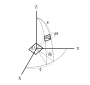
\includegraphics[width=0.7\textwidth]{images/Theory/DirectionalIntensity.pdf}
    \caption[Concept of Directional Intensity and Solid Ange]{This figure shows the concept of the directional intensity and the solid angle in e spherical coordinate system. The drawing is adapted from P.K.F. Grieder's work \cite{CosmicRayGrieder}.}
    \label{fig:DirectionalIntensityConcept}
\end{figure}
The directional intensity is often considered as a function of one of the angles, while the differential of the respective other angle gets integrated. In the case of $I_i(\phi^\prime)$, this usually results in a constant distribution. For $I_i(\theta^\prime)$, however, there is a clear angle dependence. Said zenith angle dependence can be expressed as 
\begin{equation}\label{eq:ThetaDependentIntensity}
    I_i(\theta^\prime) = I_i(\theta^\prime=\SI{0}{\degree}) \cos^{n_{i}}{(\theta^\prime)}.
\end{equation}
The parameter $n_{i}$ differs for various particles, their energies, and the elevation at which $I_i(\theta^\prime)$ is measured.

The third observable used in this work is the \textbf{differential energy spectrum}, $j(E)$. It is defined as the number of particles as a function of energy $dN_i(E)$, per unit Area, $dA$, per unit time, $dt$, per solid angle, $d\Omega^{\prime}$, and per energy interval, $dE$, \cite{CosmicRayGrieder}
\begin{equation} \label{eq:DifferentialEnergySpectrum}
    j_i(E) = \frac{dN_i(E)}{dA \, dt \, d\Omega^{\prime} \, dE}, \quad \left[ \si{\per\centi\metre\squared\per\second\per\steradian\per\giga\electronvolt} \right].
\end{equation}
The differential energy spectrum appears quite similar to the directional intensity, in fact the only noticeable difference seems to be the energy differential $dE$ in the denominator. On closer inspection though, it becomes that $dN_i(\phi^{\prime},\theta^{\prime})$ is the number of particles as a function of angles, while $dN_i(E)$ is the number of particles as a function of energy. Cosmic-ray particle energy spectra can in part be represented by a power law function in energy with a constant exponent $\gamma$ and a form factor $A$ \cite{CosmicRayGrieder}, \ie
\begin{equation} \label{eq:CosmicRayEnergyDependency}
    j(E) = AE^{-\gamma}.
\end{equation}
Therefore, most measured data is fitted to above function, often in different sections of energy. The cosmic primary particle spectrum, for example, is divided into several sections, from \SIrange{100}{3e6}{\giga\electronvolt} the exponent has a value of $\gamma \approx 2.7$. At this point, \ie at \SI{3e6}{\giga\electronvolt}, the so-called \textbf{knee} can be observed, where the dominant particle sources transitions from galactic to extra galactic. Between \SIlist{3e6;e10}{\giga\electronvolt} we find the spectrum slightly steepening from $\gamma \approx 3.0$ to $\gamma \approx 3.15$ at \SI{e9}{\giga\electronvolt}. Finally, beyond the so-called \textbf{ankle} at \SI{e10}{\giga\electronvolt} we again find $\gamma \approx 2.7$.
% TODO Make graph about the primary spectrum

In our use case, it is also interesting to consider the number of particles above a certain energy $E$. This is particularly important while studying backgrounds, since they usually appear above a certain energy threshold, so the number of background events becomes an integrated energy spectrum. For this purpose let us introduce the fourth observable, the \textbf{integral energy spectrum}, $J_i(E)$. It is defined as the integral in energy $dE^{\prime}$ from an $E$ to $\infty$ of $j_i(E^{\prime})$ as follows, \cite{CosmicRayGrieder}
\begin{equation} \label{eq:IntegralEnergySpectrum}
    J_i(E) = \int_{E}^{\infty} dE^{\prime} \ j_i(E^{\prime}) = \frac{dN_i(E^{\prime})}{dA \, dt \, d\Omega^{\prime}} \Biggr|_{E}^{\infty} \quad , \quad \left[ \si{\per\centi\metre\squared\per\second\per\steradian} \right].
\end{equation}
As can be seen, $J_i(E)$ features the same units as $I_i(\phi^{\prime},\theta^{\prime})$, but the both are indeed completely different variables introduced to show completely different purposes of cosmic-rays.

Energy spectra are often measured at different elevations, which has an impact on the form factor $A$ in equation \ref{eq:CosmicRayEnergyDependency} but does not affect the term $E^{-\gamma}$. Furthermore, astroparticle physicists do not use elevation, but \textbf{vertical depth} $X$, also known as \textbf{vertical column density} or \textbf{overburden}. It constitutes the amount of matter traversed by an incident particle along its inclined trajectory subtending a zenith angle $\theta^\prime \approx \SI{0}{\degree}$. $X$ is actually a line integral of the volume density $\rho$ and thus possesses the units of $[\si{\gram\per\centi\metre\squared}]$. Since the atmospheric density decreases exponentially with increasing elevation, our vertical depth is also an exponential function of elevation. At sea-level $X \approx \SI{1000}{\gram\per\centi\metre\squared}$, at an altitude of roughly $\SI{16}{\kilo\metre}$ \gls{asl} one finds $X \approx \SI{100}{\gram\per\centi\metre\squared}$, and $X \approx \SI{10}{\gram\per\centi\metre\squared}$ at around $\SI{32}{\kilo\metre}$ \gls{asl}. So, with every $\SI{16}{\kilo\metre}$ in elevation, $X$ is reduced by a factor of ten \cite{CosmicRayGrieder}. It is obvious, that the vertical depth must exhibit a zenith angle dependence, since a longer distance through the atmosphere has to be traversed if $\theta^{\prime} \neq \SI{0}{\degree}$. This angle dependency is introduced through the \textbf{slant depth} $X_\text{s}$ and simple trigonometry:
\begin{equation}
    X_\text{s} = \frac{X}{\cos{(\theta^\prime)}}.
\end{equation}
Above equation is only valid for $\theta^\prime \leq \SI{60}{\degree}$, where the earth's - and thus the atmosphere's curvature is negligible \cite{CosmicRayGrieder}.

For the altitude dependence let us consider intensities once again, as they show an obvious angle dependency. The intensity of a hadron $i$ measured at a vertical depth $X_1$, $I_i(\theta^\prime=\SI{0}{\degree}, X_1)$, can be transformed into $I_i(\theta^\prime=\SI{0}{\degree}, X_2)$ at a grater depth $X_2$ by \cite{CosmicRayGrieder}
\begin{equation} \label{eq:AltitudeDependency}
    I_i(\theta^\prime=\SI{0}{\degree}, X_2) = I_i(\theta^\prime=\SI{0}{\degree}, X_1) e^{-\frac{X_2-X_1}{\Lambda}}.
\end{equation}
Here, $\Lambda$ stands for the particle dependent attenuation length in units of $\si{\gram\per\centi\metre\squared}$. When using $X_\text{s}$, an angle dependence can be introduced. In addition, one can also apply above operations to energy spectra $j_i(E)$ and $J_i(E)$.

While above observables are useful to compare cosmic-ray measurements of different experiments, they are not suitable to illustrate cosmic-ray background in a single experiment like MicroBooNE. Neutrino experiments usually count events in a predetermined \textbf{fiducial volume} over a time period (see section \ref{sec:MeasuringCrossSection}). Therefore, we are, for example, not interested in the area differential. Since background cuts are applied on single variables at the time we also only consider single differentials, with the exception of $d\Omega$ which is by definition a double differential. In our case it is thus more useful to consider event rates in the \textbf{fiducial volume} $r_i$ as our base observable rather than the more complex intensities discussed above. Here the letter $i$ again denotes the particle flavour and moreover, I introduce my own notation. A rate is generally defined as
\begin{equation} \label{eq:Rate}
    r_i = \frac{dN_i}{dt}, \quad \left[ \si{\per\second} \right],
\end{equation}
where again $dN_i$ stands for the number of particles and $dt$ for the time interval. In order to accommodate different distributions, we can also introduce differential rates, analogous to the differential intensities and spectra introduced above. One of these is the \textbf{differential volume rate},
\begin{equation} \label{eq:DifferentialVolumeRate}
    \frac{dr_i(V)}{dV} = \frac{dN_i(V)}{dt \, dx \, dy \, dz}, \quad \left[ \si{\per\centi\metre\cubed\per\second} \right],
\end{equation}
with $dx$, $dy$, and $dz$ denoting the differentials of the three spacial coordinates. It is used to visualise the rate within a detector volume, wherefore one of the coordinate differentials is usually integrated, as said visualisations are often simplified to \gls{2d} views. An other often used observable of cosmic background events in a detector is their angular rate distribution, analogous to the directional intensity of equation \ref{eq:DirectionalIntensity}, and defined by
\begin{equation} \label{eq:DifferentialDirectionalRate}
    \frac{dr_i(\phi,\theta)}{d\Omega} = \frac{dN_i(\phi,\theta)}{dt \, d\phi \, d \theta \, \sin{\left(\theta\right)}}, \quad \left[ \si{\per\second\per\steradian} \right].
\end{equation}
Let us call above observable \textbf{differential directional rate}. Note that the angles $\phi$ and $\theta$ as well as the solid angle $\Omega$ now denote those of the MicroBooNE coordinate system which is rotated horizontally with respect to the astroparticle physics reference system. Analogous to the differential energy spectrum in equation \ref{eq:DifferentialEnergySpectrum} we define the \textbf{differential energy rate} as
\begin{equation} \label{eq:DifferentialEnergyRate}
    \frac{dr_i(E)}{dE} = \frac{dN_i(E)}{dt\,dE}, \quad \left[ \si{\per\second\per\giga\electronvolt} \right].
\end{equation}
Finally, let us introduce the rate equivalent of the integral energy spectrum of equation \ref{eq:IntegralEnergySpectrum}, the \textbf{integral energy rate}, $R_i$, as
\begin{equation} \label{eq:IntegralEnergyRate}
    R_i(E) = \int_{E}^{\infty} dE^{\prime} \ \frac{dr_i(E^{\prime})}{dE^{\prime}} = \frac{dN_i(E^{\prime})}{dt}\Biggr|_{E}^{\infty}\quad , \quad \left[ \si{\per\second} \right].
\end{equation}
With these parameters established, we are now ready to investigate the \gls{mc} simulation of the cosmic-ray gamma background in section \ref{sec:CosmicRayGammaBackground}.

% TODO explain that this coordinate system takes the observer as a point of reference (observing from wich angles, the radiation comes in). MicroBooNE uses the opposit: observing which angles a particle travels from the coordinate system's origin.


    % LArTPC
    % TODO Check glossary entries (textbf stuff should probably be in glossary)!
\begin{fmffile}{feynman/LArTPC} % Open the feynman graph file
\fmfset{arrow_len}{2.5mm} % smaller arrows, default 4mm
\fmfset{zigzag_width}{1thick}
\fmfset{dash_len}{1.5mm}
\chapter{Working Principle of a Liquid Argon Time Projection Chamber} \label{sec:LArTPC}
The ultimate goal of every particle physics experiment is the measurement of an incident particle's energy, momentum vector, position in the detector, and finally its identity. In this chapter, I will show how a \gls{lartpc} achieves this goal. But first I give a brief overview of the history of the \gls{lartpc} and its operating principle. After this general review, I will present the working principles of a \gls{lartpc} in detail. As I view myself as a detector physicist and this chapter is close to my heart, I tried to properly research each topic in depths. During this process, I stumbled across several shortcomings and inconsistencies in our field which might be worthy of future studies.

In 1974 D. R. Nygren proposed a novel concept of a particle detector \cite{TPCProposal} to be built for the \gls{pep} collider experiment \cite{TPCExperiment} at \gls{slac}. The aim of this revolutionary detector setup was to provide a $4\pi$, truly 3-dimensional data signature with high spacial resolution, unambiguous spacial reconstruction and high data rate capability. In essence, Nygren's design was an ingenious application of a \gls{mwpc} \cite{TPCPredecessor} placed at the end of a large drift volume of methane gas as detector medium \cite{TPCDescription}, thus reducing the number of channels and simplifying reconstruction. He named his invention \gls{tpc}. Three years later C. Rubbia proposed the use of \gls{lar} as detector medium \cite{LArTPCProposal}, since it offers much higher density as methane gas. These \glspl{lartpc} can thus be used for low cross section experiments \eg neutrino detection. Moreover, \gls{lar}'s high density also provides a relatively high mass stopping power, and therefore excellent calorimeteric properties. As Argon is the third most abundant gas in our atmosphere and easily purified, its liquid form is available in large quantities for a low prise \cite{NobleGasDetectors}. These, and various other important properties of \gls{lar}, listed in table \ref{tab:LArProperties}, make it the material of choice for current and future neutrino experiments. Then, in 1982, P.J. Doe, H.-J. Mahler, and H.H. Chen built and operated the first \gls{lartpc}, measuring tracks in two dimensions (only one wire-plane) \cite{LArTPCFirst}. Three years later Rubbia and the ICARUS collaboration proposed the first large scale \glspl{lartpc} to be situated in the Gran Sasso Laboratory deep underground \cite{ICARUSProposal}. This marked the beginning of various important developments in material testing and cryogenics by said collaboration, resulting in the modular ICARUS T600 detector commissioned in 2004 \cite{ICARUST600}. The ICARUS T600 consisted of two T300 modules with a total active detector mass of \SI{476}{\tonne}. All large scale designs following ICARUS were heavily influence by this detector design, and so was MicroBooNE, although not matching the uncompromising build quality of ICARUS. 
% TODO Add more history: Argontube? ArDM?

Before a \gls{lartpc} can be operated, the detector medium, \gls{lar}, needs to be contained and kept at constant temperature. Therefore, thermally insulated cryogenic steel vessels of various designs are used. In these vessels the \gls{tpc} usually rests on electrically insulating holding structures. Every \gls{tpc} has a so-called \textbf{active volume} in its core, filled with the detector medium, like \gls{lar}, where the particle interactions take place. In said active volume a constant and uniform electric field is applied between an anode and a cathode, wherefore a field cage surrounding the active volume is employed. The field cage is usually charged by a \gls{dc} \gls{hv}, fed through the cryogenic vessel and stepped down by resistors between every field cage stage. A \gls{tpc}'s anode also acts as its readout system. So far, all large scale detectors employ multi-wire planes able to measure the charge of particle's ionisation traces. Finally, \glspl{lartpc} feature a light readout system, usually consisting of \glspl{pmt}. A schematic view of an above described \gls{lartpc} is shown in figure \ref{fig:TPCSchematics}.
\begin{figure}[htbp]
    \centering
    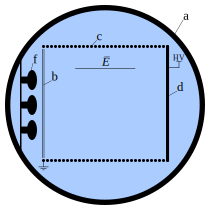
\includegraphics[width=0.9\textwidth]{images/Detector/TPCSchematics.pdf}
    \caption[Schematic view of a LArTPC]{Schematic side view of a \gls{lartpc}. In this picture, \textbf{a} is the vessel containing the \gls{lar} (light blue) and the \gls{tpc}. At letter \textbf{b} the readout planes are positioned, in this case depicted as three wire planes in various orientations. The readout planes also act as the anode of the \gls{tpc}. Labelled by \textbf{c}, one finds the field cage comprised of single steel tubes connected by a voltage divider, \ie the voltage decreases with every tube towards the anode. The cathode is labelled by \textbf{d}, so \textbf{b} through \textbf{d} show all the components of a \gls{tpc} and enclose the active volume. Applying a negative \gls{hv} to the cathode introduces an uniform electric field $\vec{E}$ pointing from the anode to the cathode. Finally, \textbf{f} shows the light readout system, in this case an array of \glspl{pmt}.}
    \label{fig:TPCSchematics}
\end{figure}

As a charged particle traverses the active volume it ionises the detection medium (\gls{lar}) along its trajectory and also creates excited states, see figure \ref{fig:TPCFunction1}. Thereupon a fraction of the resulting electron-ion pairs recombine and thus produce more excited states. Most of these then decay under the emission of scintillation light, while some come in contact with impurities and decay emitting heat. The whole recombination and scintillation process occurs within a time scale of nanoseconds. A light readout system, historically consisting of multiple \glspl{pmt}, is then used to detect said light emission in order to determine the time $t_0$ of the incident particle crossing the active volume. These recombination and scintillation mechanisms are all shown in figure \ref{fig:TPCFunction2}. Yet, the electric field $\vec{E}$ prevents a full recombination and lets the electrons drift towards the anode with a constant velocity $v_\text{d}$ and the ions, although much slower, towards the cathode. During the drift, some of the electrons get captured by impurities, as depicted figure \ref{fig:TPCFunction3}. When the electrons reach the anode, the readout wire planes detect the drift charges, as visualised in figure \ref{fig:TPCFunction4}. These wire plane signals are then used to measure the \gls{2d} positioning $(y,z)$, timing $t$, and intensity of the incoming drift electrons. The electron drift time, $t-t_0$, is of the order milliseconds for large scale detectors. Knowing the drift velocity $v_\text{d}$, $t-t_0$ can be used to calculate the missing coordinate $x = v_\text{d}(t-t_0)$ and thus, in combination with the \gls{2d} positioning, one obtains a \gls{3d} interaction picture $(x,y,z)$ of the incident particles. Furthermore, the measured charge intensity facilitates particle identification and calorimetry. In the following subsections the abovementioned working principle of a \gls{lartpc} will be discussed in depth, based on the works of E. Aprile, A. E. Bolotnikov, A. I. Bolozdnya, and T. Doke \cite{NobleGasDetectors} as well as V. Chepel and H. Ara\'ujo \cite{NobleGasDetectorsBetter}.
\begin{figure}[htbp]
    \centering
    \subfloat[Ionisation and Excitation][Ionisation and excitation]
    {
        \includegraphics[width=0.48\textwidth]{images/Detector/TPCFunction1.pdf}
        \label{fig:TPCFunction1}
    } %\qquad
    \subfloat[Recombination and Scintillation][Recombination and scintillation]
    {
        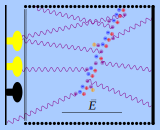
\includegraphics[width=0.48\textwidth]{images/Detector/TPCFunction2.pdf}
        \label{fig:TPCFunction2}
    } \\
    \subfloat[Electron- and Ion Drift][Electron- and ion drift]
    {
        \includegraphics[width=0.48\textwidth]{images/Detector/TPCFunction3.pdf}
        \label{fig:TPCFunction3}
    } %\qquad
    \subfloat[Charge Signal Readout][Charge signal readout]
    {
        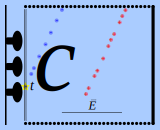
\includegraphics[width=0.48\textwidth]{images/Detector/TPCFunction4.pdf}
        \label{fig:TPCFunction4}
    }
    \caption[Working Principle of a Liquid Argon TPC]{In the above figures the working principle of a \gls{lartpc} is illustrated. In \subref{fig:TPCFunction1} the ionisation and excitation process is depicted, as a charged particle enters the active volume, with its trajectory illustrated in green. Along said trajectory electrons (blue spots), argon ions (red spots), and excited states of argon (purple spots) are created by the incident particle's energy deposition. Image \subref{fig:TPCFunction2} shows the recombination- and scintillation light creation processes. Here, some of the electrons and ions recombine to form more excited states, but the electric field $\vec{E}$ prevents all of them from recombining. Almost instantly a majority of the excited states are involved in the production of scintillation photons (purple wavy lines), while some are quenched by impurities (orange spots) or argon ions. If the photons hit the \glspl{pmt} of the light readout system, these then generate a time signal $t_0$ (indicated as yellow \glspl{pmt}). In \subref{fig:TPCFunction3} the electron and ion drift are depicted. While the electron drift, due to $\vec{E}$, with a constant velocity $v_\text{d}$ towards the anode, they sometimes get captured by impurities with a high \gls{electronegativity} (orange spots) and are thus becoming useless for the charge signal measurement. The argon ions drift much slower towards the cathode. Finally, depicted in \subref{fig:TPCFunction4} is the charge signal creation at the readout plane. When the electrons reach the readout plane at the anode end of the \gls{tpc}, they generate a signal (yellow star) in \gls{2d} space $(y,z)$, arrival time $t$, and amount of charge. The arrival time can be used in combination with $t_0$ and $v_\text{d}$ to reconstruct the third spacial component $x = v_\text{d}(t-t0)$. The resulting signal is a \gls{3d} picture, $(x,y,z)$, of the incident particle track and its energy deposition.}
    \label{fig:TPCFunction}
\end{figure}

\section{Liquid Argon Properties}
There are several advantageous properties of \gls{lar} which makes it preferable for the use as a \gls{tpc} medium. Most notably, noble gases like argon are inert substances featuring a fully occupied valence shell. Therefore they neither bond with, nor attract \glspl{quasifreeelectron}. Heavy noble liquids and solids (argon, krypton, and xenon) feature a high polarisability, thus allowing for \glspl{quasifreeelectron} to drift with high velocities. This property allows for long drift distances (tens of meters). Another advantages property of noble liquids in general is their translucence to their own scintillation light. In all the aforementioned properties xenon excels all the other noble liquids, but argon is the third most abundant gas in the atmosphere and thus the noble gas with the lowest cost associated to it. This makes \gls{lar} the only affordable option for the use in multi-kiloton detectors.

However, there are also several challenges associated with the use of \gls{lar}. A major concern is the relatively low \gls{bp} of $T_{\text{b}}=\SI{87.303(2)}{\kelvin}$ at standard pressure. This requires the utilisation of complicated cryogenic systems in order to establish a controlled detector environment. Furthermore, with a \gls{mp} of $T_{\text{m}} = \SI{83.8(3)}{\kelvin}$ the temperature range of the liquid state amounts only to \SI{3.5(3)}{\kelvin}, which further complicates the cryogenic requirements. The thermodynamic properties argon are listed in table \ref{tab:LArProperties} and shown in the phase diagram in figure \ref{fig:PhaseDiagram}.
\begin{figure}[htbp]
    \centering
    \includegraphics[width=0.9\textwidth]{images/Detector/PhaseDiagramArgon.pdf}
    \caption[Phase Diagram of Argon]{Phase diagram of argon in the temperature-pressure space in the ranges of \SIrange{60}{180}{\kelvin} and \SIrange{1e-2}{1e4}{\bar}. The lines of phase changes are drawn in colour and the standard pressure as a dashed line at \SI{1}{\bar}. Where the latter crosses the phase change lines the \acrfull{bp} and \acrfull{mp} are highlighted. The \acrfull{tp} and \acrfull{cp} are shown as well. Formulas and values were sourced from \cite{ArgonProperties2,ArgonProperties3}.}
    \label{fig:PhaseDiagram}
\end{figure}
Other difficulties are not posed by the \gls{lar} itself, but by three impurity types: 
\begin{itemize}
    \item Radioactive isotopes, which mimic low energy light and charge signals. These consist mostly of radon introduced through outgassing of contaminated solids like glass. Another source of radio activity is posed by radioactive argon isotopes, most prominently \ce{^39Ar} with a $T_{1/2}=\SI{269(3)}{\year}$ \cite{IsotopeData}. 
    \item Scintillation light quenching impurities, which reduce the light intensity measured by the light readout system. During standard operations the main contributor for this is nitrogen \ce{N2}.
    \item Charge binding impurities which reduce the charge collected by the readout. These are mostly molecules composed of atoms with high \gls{electronegativity} like \ce{O2} or \ce{H2O}.
\end{itemize}
However, all these operational difficulties can be controlled by filtering techniques, smart choice of materials, underground argon, and cleanliness during installation. Thus \gls{lar} serves as an excellent detector medium in \glspl{tpc}. The \gls{lar} properties most essential for \gls{lartpc} operations are listed in table \ref{tab:LArProperties}.

In regards of safety, the low \gls{bp} of argon may lead to fast pressurisation of any storage vessel. This could lead to catastrophic explosions if left unmitigated. Thus safety release valves and rupture discs, which vent the gas in an emergency, are paramount for safe \gls{lartpc} operations. In gas form, argon's high density lets it displace air and creating an oxygen deficiency hazard in underground facilities and other confined spaces. This is mitigated by workers safety training, wearing of oxygen monitors, as well as ventilation systems providing a safe path to emergency exits. It is therefore possible to safely operate even large scale \glspl{lartpc}.

\begin{table}[hbtp]
    \centering
    \caption[Properties of Liquid Argon]{Properties of liquid argon. For the mean excitation energy only the value of the gas phase is available (for liquid \ce{H2} it is increased by $\sim\SI{14}{\percent}$ compared to gas \cite{StoppingPowerNumbers}). The acronym \acrshort{mip} stands for \acrlong{mip} which will be explained later in this chapter.}
    \begin{tabu} to 0.7\textwidth{lcrlc} \toprule
        \rowfont[c]{\bf} Variable & Symbol & Value & Unit & Source\\ \midrule
        Atomic number & $Z$ & 18 & & \cite{ArgonProperties1}\\
        Molecular weight & $A$ & \num[separate-uncertainty = false]{39.948(1)} & \si{\gram\per\mol} & \cite{ArgonProperties1} \\
        \Acrfull{bp} at \SI{1}{\bar}& $T_{\text{b}}$ & \num[separate-uncertainty = false]{87.303(2)} & \si{\kelvin} & \cite{ArgonProperties2} \\
        \Acrfull{mp} at \SI{1}{\bar}& $T_{\text{m}}$ & \num[separate-uncertainty = false]{83.8(3)} & \si{\kelvin} & \cite{ArgonProperties3} \\ 
        Density at \SI{1}{\bar} \gls{bp} & $\rho$ & \num{1.39646} & \si{\gram\per\centi\metre\cubed} & \cite{ArgonProperties2} \\ 
        Viscosity at \SI{1}{\bar} \gls{bp} & $\eta$ & \num[separate-uncertainty = false]{273.2(55)} & \si{\micro\pascal\second} & \cite{NistChemistryWebBook} \\ 
        Sound velocity at \SI{1}{\bar} \gls{bp} & $c_\text{s}$ & \num[separate-uncertainty = false]{842.9(84)} & \si{\metre\per\second} & \cite{NistChemistryWebBook} \\ \midrule
        \multirow{2}{*}{\Acrfull{tp}} & $T_{\text{t}}$ & \num{83.8058} & \si{\kelvin} & \multirow{2}{*}{\cite{ArgonProperties2}} \\
                                      & $p_{\text{t}}$ & \num[separate-uncertainty = false]{0.68891(2)} & \si{\kilo\pascal} & \\ \midrule
        \multirow{2}{*}{\Acrfull{cp}} & $T_{\text{c}}$ & \num[separate-uncertainty = false]{150.687(15)} & \si{\kelvin} & \multirow{2}{*}{\cite{ArgonProperties2}}  \\
                                      & $p_{\text{c}}$ & \num[separate-uncertainty = false]{48.63(3)} & \si{\bar} &  \\ \midrule
        Ionisation energy (gas) & $I_\text{GAr}$ & \num[separate-uncertainty = false]{15.7596099(7)} & \si{\electronvolt} & \cite{ArgonIonisationEnergy}\\
        Ionisation energy (liquid) & $I_{\text{LAr}}$ & \num{13.4} & \si{\electronvolt} & \cite{NobleGasDetectors} \\
        W-value of ionisation & $W_\text{i}$ & \num[separate-uncertainty = false]{23.6(3)} & \si{\electronvolt} & \cite{LArW-Value,LArW-ValueErratum} \\
        W-value of scintillation (max) & $W_\text{ph}(\text{max})$ & \num[separate-uncertainty = false]{19.5(10)} & \si{\electronvolt} & \cite{LArWScint-Value1,LArWScint-Value2} \\
        W-value of scint. (\acrshort{mip}) & $W_\text{ph}(\text{MIP})$ & \num[separate-uncertainty = false]{25.1(25)} & \si{\electronvolt} & \cite{LArWScint-Value1,LArWScint-Value2} \\
        Scintillation wave length & $\lambda_\text{sc}$ & \num[separate-uncertainty = false]{128(10)} & \si{\nano\metre} & \cite{LArScintillationSpectrum1,LArScintillationSpectrum2} \\
        Mean excitation Energy (gas) & $I_{\text{ex}}$ & \num[separate-uncertainty = false]{188(10)} & \si{\electronvolt} & \cite{StoppingPowerNumbers} \\
        Critical Energy of $e^{-}$ & $E_\text{c}$ & \num{32.84} & \si{\mega\electronvolt} & \cite{PDGMaterialProperties} \\
        Radiation length & $X_0$ & \num{19.55} & \si{\gram\per\centi\metre\squared} & \cite{PDGMaterialProperties} \\ %TODO check if more reliable source?
        Dielectric constant & $\epsilon_\text{r}$  & \num[separate-uncertainty = false]{1.504(1)} & & \cite{LArDielectricConstant} \\
        Refractive index at \SI{546.1}{\nano\metre} & $n$  & \num[separate-uncertainty = false]{1.2278(12)} & & \cite{LArRefractiveIndex} \\
        Moli\`{e}re radius & $R_\text{m}$ & \num{9.043} & \si{\centi\metre} & \cite{PDGMaterialProperties} \\
        \acrshort{mip} linear stopping power & $\left\langle -\frac{dE}{dx} \right\rangle_\text{MIP}$ & \num{2.105} & \si{\mega\electronvolt\per\centi\metre} & \cite{PDGMaterialProperties} \\
        \bottomrule
    \end{tabu}
    \label{tab:LArProperties}
\end{table}
% TODO sort table!!!!!

% Particles in Argon
\section{Excitation and Ionisation of Liquid Argon} \label{sec:ParticleInteractions}
Only charged particles can be directly observed in a \gls{lartpc}, as they interact with the detector medium through Coulomb forces. In essence, there are three immediate effects a charged particle, here denoted as \ce{X^{$\pm$}}, has on an argon atom \ce{Ar}. The first and lowest energy process, is the excitation of the atom, denoted by \ch{Ar^*}. The second interaction mode, requiring more energy than excitation, is producing an electron-ion pair, \ie ionisation. The resulting charged ion is represented by the symbol \ce{Ar^+}. Finally there is the spallation of the atom by direct interaction with its core. This produces a multitude, \ia of charged particles, which are again subject to the former two interactions. However, spallation requires many orders of magnitudes more energy (at least several \SI{100}{\mega\electronvolt}) than ionisation (around \SI{10}{\electronvolt}) or excitation (several \si{\electronvolt}). In this work, I will present the latter two interactions, and omit an in depth discussion of spallation. 

The ionisation, as mentioned before, is induced by a charged particle, \ce{X^{$\pm$}}, transferring momentum to an electron, in the shell of an argon atom, \ce{Ar}, by the means of the \gls{em} force. Consequently, the electron overcomes the Coulomb-potential of the atom which results in a \gls{quasifreeelectron} $e^-$ and a positively charged argon ion \ce{Ar^+}. We can thus express said process by
\begin{equation} \label{eq:IonisationProcess}
    \ce{Ar + $X^{\pm}$ -> Ar^+ + $e^-$ + $X^{\prime\pm}$}.
\end{equation}
In this case, \ce{X^{$\prime\pm$}} stands for the ionising particle \ce{X^{$\pm$}} after the energy loss. The excitation process is very similar with the difference that the transferred energy is too low to overcome the Coulomb-potential and thus placing the electron only on a higher energy eigenstate, \ie an excited state. The production of an excited argon atom \ch{Ar^*} can be described as
\begin{equation} \label{eq:ExcitationProcess}
    \ce{Ar + $X^{\pm}$ -> \ch{Ar^*} + $X^{\prime\pm}$}.
\end{equation}
In addition there are also occurrences of multiply ionised states \ce{Ar^{$n$+}}, excited ionised states \ch{Ar^{+*}}, as well as combinations of the two:
\begin{align} \label{eq:SecondaryIonProcess}
    \ce{Ar + $X^{\pm}$ &-> Ar^{$n$+} + $n e^-$ + $X^{\prime\pm}$}, \nonumber \\
    \ce{Ar + $X^{\pm}$ &-> \ch{Ar^{+*}} + $e^-$ + $X^{\prime\pm}$}, \\
    \ce{Ar + $X^{\pm}$ &-> \ch{Ar^{$n$+*}} + $n e^-$ + $X^{\prime\pm}$}. \nonumber
\end{align}
In a Feynman diagram the ionisation and excitation processes look the same, for both are momentum transfers from $X^{\pm}$ to the electron $e^-$ in the atomic shell. The momentum is transferred by a photon as illustrated in figure \ref{fig:IonisationAndExcitation}.
\begin{figure}[htbp]
    \centering
    \fmfframe(10,10)(0,10){
        \begin{fmfgraph*}(120,80)
            \fmfleft{i1,i2}
            \fmfright{o1,o2}
            \fmf{fermion}{i1,v1,o1}
            \fmf{fermion}{i2,v2,o2}
            \fmf{photon,label=$\gamma$,label.side=left,label.dist=0.1cm}{v1,v2}
            \marrow{photm}{right}{rt}{$p$}{v2,v1}
            \fmfv{label=$e^-$,label.angle=180,label.dist=0.1cm}{i1}
            \fmfv{label=$X^\pm$,label.angle=180,label.dist=0.1cm}{i2}
            \fmfv{label=$e^-$,label.angle=0,label.dist=0.1cm}{o1}
            \fmfv{label=$X^{\prime\pm}$,label.angle=0,label.dist=0.1cm}{o2}
            \fmfv{decor.shape=circle,decor.filled=full,decor.size=1thick}{v1}
            \fmfv{decor.shape=circle,decor.filled=full,decor.size=1thick}{v2}
        \end{fmfgraph*}
    }
    \caption[Feynman Diagrams of Ionisation and Excitation]{This figure depicts the Feynman diagrams of the ionisation and excitation process. In processes the momentum $p$ is transferred from a charged particle $X^{\pm}$ to a shell electron $e^-$ by a photon $\gamma$.}
    \label{fig:IonisationAndExcitation}
\end{figure}

The rate of ionisation or excitation is not only depending on the momentum transferred by the charged particle, but also by the ionisation potential and resonant energy levels of \gls{lar} as well as their structure. In a condensed, non-polarised, dense fluid, like \gls{lar}, one observes a reduction in ionisation energy compared to their gas state, \ie  $I_\text{liquid} < I_\text{gas}$. This is attributed to three effects:
\begin{enumerate}
    \item The conduction band of the quasi-free electrons widens, thus, effectively reducing the ionisation threshold by the band's width $V_0$.
    \item The higher atomic density of a liquid leads to an increase of the dielectric constant $\epsilon_\text{r}$, hence, raising the polarisability of the single atoms. This elevates the ground state energy of the valence electrons by the polarisation energy $P_+$.
    \item The valence electron energy levels develop into valence bands, increasing the ground state energy by the band's width $E_\text{val}$.
\end{enumerate}
With this information we can now form a rather simple equation for calculating the ionisation energy of a non-polarised liquid \cite{LArIonisationEnergy1},
\begin{equation} \label{eq:LiquidIonisationEnergy}
    I_\text{liquid} = I_\text{gas} + V_0 + P_+ + E_\text{val}.
\end{equation}
Here the signs are positive by convention, and thus, $V_0$, $P_+$, and $E_\text{val}$ all take negative values. Above effects and equation are schematically depicted in figure \ref{fig:LArIonisationPotential}.
\begin{figure}[htbp]
    \centering
    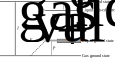
\includegraphics[width=0.9\textwidth]{images/Detector/LArIonisationPotential.pdf}     
    \caption[Changes in the Ionisation Energy Induced by Condensation]{This picture shows a schematic representation of the changes to the ionisation energy induced by condensation. In non-polarised liquids the ionisation energy is reduced compared to the gas state, $I_\text{liquid} < I_\text{gas}$. This is explained by the reduction of the ground state energy of quasi-free electrons $V_0$, the increase of the ground state energy level by the polarisation energy $P_+$, and the development of valence band with a width of $E_\text{val}$. The band gaps in above depiction are not to scale. This graph is inspired by \cite{LArIonisationEnergy2}.}
    \label{fig:LArIonisationPotential}
\end{figure}
By far the largest contributing factor to the ionisation energy shift is the polarisation energy $P_+$ typically ranging between \SIrange{1}{2}{\electronvolt} \cite{LArIonisationEnergy2}. $P_+$ can be derived employing the Born equation \cite{BornEquation} which is just the difference between the potential energies of a singly charged sphere with radius $r_+$ in vacuum $W(\epsilon_0)$ and in a medium $W(\epsilon_0\epsilon_\text{r})$:
\begin{equation}
    P_+ = \frac{1}{2} \left( W(\epsilon_0\epsilon_\text{r}) - W(\epsilon_0) \right) = - \frac{e^2}{8 \pi \epsilon_0 r_+} \left( 1 - \frac{1}{\epsilon_\text{r}} \right).
\end{equation}
Here $\epsilon_\text{r}$ denotes the dielectric constant of the medium, in our case \gls{lar}, $\epsilon_0$ the vacuum permittivity, and $e$ the electron charge. Besides these often used constants there is also $r_+$ which stand for the radius of a singly ionised atom of the medium. Above equation indicates that the $P_+$ correction is just the classical approximation of the behaviour of the outermost electron in the ion's potential while changing the dielectric constant. Note that, according to equation \ref{eq:LiquidIonisationEnergy}, this classical correction is then applied to shift quantum mechanical energy eigenstates; quite an oddity in physics. As for $V_0$ and $E_\text{val}$, these both have to be measured and their values are usually one order of magnitude smaller than $P_+$. In addition to the shift in ionisation potentials, when condensing a gas into a liquid, the excited states are also affected. Their energy levels are shifted by the same energy difference $\Delta I = I_\text{liquid} - I_\text{gas}$. Furthermore, the levels also broaden and form bands, just like the ground state valence band \cite{LArIonisationEnergy2}.

In the case of \gls{lar}, one finds $V_0 = \SI{-0.21(2)}{\electronvolt}$ and $E_\text{val} = \SI{0.1}{\electronvolt}$ \cite{LArQuasiFreeBandWidth}. Furthermore, the ionisation potential of the gas state is measured as $I_\text{GAr} = \SI{15.76}{\electronvolt}$ \cite{ArgonIonisationEnergy}. Performing above calculations results in a liquid state ionisation potential of $I_\text{LAr} = \SI{13.4}{\electronvolt}$ \cite{NobleGasDetectors}. Thus, the excited states are shifted by $\Delta I = \SI{-2.36}{\electronvolt}$. In addition, the band width of the excited states of \gls{lar} have a full width half maximum of \SI{0.08}{\electronvolt} \cite{LArExcitationBandWidth}. All the above effects are illustrated in figure \ref{fig:ArEnergyLevels} with the gas energy levels shown in \subref{fig:ArEnergyLevelsGas} and the energy bands of \gls{lar} depicted in \subref{fig:ArEnergyLevelsLiquid}.
\begin{figure}[htbp]
    \centering
    \subfloat[Energy Levels of Gaseous Argon][Energy levels of gaseous argon]
    {
        \includegraphics[width=0.49\textwidth]{images/Detector/ArEnergyLevelsGas.pdf}
        \label{fig:ArEnergyLevelsGas}
    } %\qquad
    \subfloat[Energy Levels of Liquid Argon][Energy Bands of \gls{lar}]
    {
        \includegraphics[width=0.49\textwidth]{images/Detector/ArEnergyLevelsLiquid.pdf}
        \label{fig:ArEnergyLevelsLiquid}
    }
    \caption[Energy Levels in Gaseous and Liquid Argon]{The above pictures illustrate the difference in energy levels in gaseous and liquid argon. Exited states with a odd total angular momentum $J$ are drawn in red, while the ones with an even $J$ are shown in blue. The ground state and the ionised state are represented by black lines. In \subref{fig:ArEnergyLevelsGas} the energy levels of argon gas are depicted as thin lines sourced from \cite{ArgonIonisationEnergy,ArgonEnergyLevels1}. Image \subref{fig:ArEnergyLevelsLiquid} shows the energy bands of \gls{lar}. This graph was produced by using the same data as in \subref{fig:ArEnergyLevelsGas}, adjusting the levels by $\Delta I = \SI{-2.36}{\electronvolt}$, and broadening the thin lines into bands with a width of two times \SI{0.08}{\electronvolt}. The excited states are displayed in transparent colours in order to illustrate the overlapping of various states. Also, the ground state was changed to a band with its upper edge at \SI{0}{\electronvolt}. The ionised state is still depicted as a line, since it embodies more of a threshold than an eigenstate state anyway.}
    \label{fig:ArEnergyLevels}
\end{figure}
% TODO make energy levels different color for J = 0, 1, 2, 3, 4? Maybe not?

\section{Ionisation Yield of Charged Particles in Liquid Argon}
In order to determine a charged particle's deposited energy in \gls{lar} one first needs to determine the mean energy expended in \gls{lar} per electron-ion pair formed. Said mean energy is called \textbf{W-value}, or $W_\text{i}$, which shall not be mistaken with the ionisation potential $I_\text{LAr}$. As we have seen above in section \ref{sec:ParticleInteractions}, a particle's dissipated energy is not exclusively expended in the ionisation processes. In general, these ionisation inefficiencies lead to a higher energy requirement compared to the ionisation potential, \ie $W_\text{i} > I_\text{LAr}$. In the following we will discuss said inefficiencies as well as the derivation and measurement of $W_\text{i}$. 

According to R.L. Platzman \cite{W-ValueGeneralCalculation} the energy $E$ of an incident particle stopped in a gas has to adhere to the following energy balance: 
\begin{equation} \label{eq:IonisationEnergyBallance}
    E = N\bar{E}_{\text{i}} + N_{\text{ex}}\bar{E}_{\text{ex}} + N\bar{\epsilon}_{\text{i}},
\end{equation}
where $N$ stands for the total number of electron-ion pairs produced and $N_{\text{ex}}$ is the number of excited states produced. $\bar{E}_{\text{i}}$ denotes the mean energy expenditure of the ionisation process, which includes the creation of multiple charged, and excited charged states and thus exceeds the ionisation potential $I_\text{LAr}$. $\bar{E}_{\text{ex}}$ signifies the average energy expenditure for the production of excited states, and $\bar{\epsilon}_{\text{i}}$ is the average kinetic energy of the \glspl{quasifreeelectron} produced in the ionisation process. Note, that the last-mentioned energy is too low to further ionise or excite the detector medium. If we recall the meaning of the W-value, as the energy to produce a single electron-ion pair, we find that it is simply defined by dividing equation \ref{eq:IonisationEnergyBallance} by $N$, so we get
\begin{equation} \label{eq:W-ValueDefinition}
    W_\text{i} \coloneqq \frac{E}{N} = \bar{E}_{\text{i}} + \frac{N_{\text{ex}}}{N}\bar{E}_{\text{ex}} + \bar{\epsilon}_{\text{i}}.
\end{equation}
Theoretical calculations hint to an asymptotic behaviour of $W_\text{i}$ with increasing particle energy, $E$. Therefore, $W_\text{i}$ is expected to be constant for $E \gg I_\text{LAr}$ \cite{W-ValueAsymptotic}. This energy requirement is certainly given in all \gls{lartpc} applications as typical lower energy limits are of the order of \si{\mega\electronvolt}. Based on measurements in various gasses it is assumed that $W_\text{i}$ is constant for different kinds of particles. A comparison of \SI{1.8}{\mega\electronvolt} \textalpha-particles with \SI{5.3}{\mega\electronvolt} protons in argon gas for example found a ratio of $W_{\alpha}/W_p = 0.990$. This and measurements with heavy ions suggest that $W_\text{i}$ is independent of mass or charge of the incident particles at high enough energies \cite{W-ValueGeneralSummary}. One proven dependency, however, is introduced by the density and thus pressure and temperature, since A. Bolotnikov and B. Ramsey showed a clear temperature and density dependence of the W-value in pressurised xenon gas \cite{W-ValueDensityDependency}.

Platzman's equation \ref{eq:IonisationEnergyBallance} was introduced to calculate $W_\text{i}$ for gasses, but ultimately it is also valid for noble liquids, \eg \gls{lar}, and only the values of the variables are different. In general the ionisation yield of noble liquids is found to be greater than in the gas phase and thus the value of $W_\text{i}$ of liquids is lower \cite{W-ValueLiquids}. According to Takahashi \etal \cite{W-ValueLiquidAndGas} the ratio $W_\text{i}/I_\text{LAr}$ is constant and thus the lower W-value can be explained with the lower ionisation potential in the liquid state, \ie $I_\text{gas} > I_\text{liquid}$. For \gls{lar} the W-Value was measured by M. Miyajima \etal \cite{LArW-Value,LArW-ValueErratum} as 
\begin{equation} \label{eq:W-ValueLar}
    W_\text{i} = \SI{23.6(3)}{\electronvolt}. 
\end{equation}
They used a \ce{^{207}Bi} source emitting \textbeta-radiation with energies at \SIlist[list-units = single]{0.48;0.55;0.976;1.05}{\mega\electronvolt}. Furthermore, the ionisation chamber of the experiment seemed to be pressurised at \SI{1.8}{\atmosphere} and no \gls{lar} temperature was provided. From the W-value we can easily calculate the ionisation efficiency in \gls{lar} as
\begin{equation}
    \varepsilon_\text{ion} = \frac{I_\text{LAr}}{W_\text{i}} = \SI{56.8}{\percent}.
\end{equation}

Looking at large collections of W-values of various particles in noble gasses and liquids \cite{W-ValueGeneralSummary,W-ValueLiquids} three things are apparent: First, all measurements of W-values are all quite dated and thus limited to technologies available in the 1960s and 1970s. Second, they were performed using radioactive sources with well defined decay spectra or, in case of protons and heavy ions, making use of low energy beams and are thus limited in energy range, typically between \si{\kilo\electronvolt} and several \si{\mega\electronvolt}. Third, there are no measurements of the W-values for \glspl{Meson} or muons. In the case of \gls{lar} there is only electron related data. Furthermore, it is unclear if density is affecting the value of $W_\text{i}$ and thus if there is pressure and temperature dependence. Nevertheless, the \gls{lar} value of $W_\text{i}$ shown in equation \ref{eq:W-ValueLar} is the standard used in every \gls{lartpc} based experiment.

In my personal opinion the W-value's derivation, by means of limited measurements, bases on a chain of various bold assumptions:
\begin{enumerate}
    \item The data for gasses shows hints of an asymptotic behaviour of $W_\text{i}$ with high energies and we assume this to be true for even higher energies than actually measured.
    \item We further assume, that $W_\text{i}$ shows this asymptotic behaviour for all particles.
    \item Then we even assume, based on a limited amount of data points, that this asymptotic limit of $W_\text{i}$ has the same value for all charged particles even the \glspl{Meson} or muons that were never used in a measurement.
    \item Furthermore, we assume all of the above to be true in noble liquids and not just gasses.
    \item And finally, we ignore a possible density dependence of $W_\text{i}$ although theories suggest otherwise.
\end{enumerate}
Some of these points were already raised in an ICRU Report of 1979 stating: \cite[ \lbrack ...\rbrack \textit{measurements of W have so far been carried out with a limited variety of particles, e.g., electrons, protons, alpha particles and some heavy ions at selected kinetic energies. Extensive mapping of the energy dependence of W is highly desirable both for basic understanding and for application.} \lbrack ...\rbrack \textit{the variation of the W value with gas conditions for a particular incident particle must be thoroughly investigated.} \lbrack ...\rbrack \textit{Current theory suggests the presence of pressure dependence even in pure gases, especially in the neighborhood of 1 kPa.} \lbrack ...\rbrack \textit{It is commonly believed, largely on theoretical grounds, that $W$ for any charged particle should approach an asymptotic value at sufficiently high kinetic energies. But it is unknown how much difference there is between W values of protons at different energies.}]{W-ValueGeneralSummary}. Yet the \gls{lartpc} community never addressed these issues. Even worse, we stopped questioning the only measurement of the \gls{lar} W-value and started to rely on it as it were some kind of natural constant. I think in view of a large scale \gls{lartpc} experiments it is time to properly address this issue and remeasure $W_\text{i}$ of \gls{lar}, using modern technology and various particle beams in energy ranges that actually matter for modern experiments. In addition the effects of temperature, pressure, and thus, density on the W-value should be determined as well. 
% TODO Calculate: This leads to an ionization yield of about \SI{6e3}{e^{-}\per\milli\metre} for minimum ionizing muons and an electric field of \SI{1}{\kilo\volt\per\centi\metre}.
% TODO Move this into the ionisation subsection above?

% Laser Ionisation
\section{Energy Dissipation of Charged Particles} \label{sec:EnergyDissipationCharged}
Thus far, we only considered energy loss from the perspective of the detector medium and how it is affected by energy deposited by charged particles. But in order to be able to reconstruct particle traces measured by a \gls{lartpc}, we also need to consider how particles interact and deposit energy in \gls{lar}. Charged massive particles dissipated their energy in the absorber medium in two different modes. The most dominant for particles with $0.1 \lesssim \beta\gamma \lesssim 1000$, \ie moderately relativistic particles, is ionisation. Said ionisation loss is described by the \textbf{Bethe equation} \cite{PDG2018}
\begin{equation}\label{eq:BetheBloch}
    \frac{1}{\rho} \left\langle -\frac{dE}{dx} \right\rangle_{\text{Ion}} = \frac{4 \pi \hbar^2 \alpha^2 N_A}{m_e} \frac{z^2}{\beta^2} \frac{Z}{A} 
    \left( \frac{1}{2} \ln \left( \frac{2 m_e c^2 \beta^2 \gamma^2 W_{\text{max}}}{I^2_\text{ex}} \right) - \beta^2 - \frac{\delta(\beta\gamma)}{2} \right).
\end{equation}
The whole therm on the left side of the equation is often called \textbf{mass stopping power}, whereas $\langle -dE/dx\rangle$ is called \textbf{linear stopping power}. The latter is defined as the mean energy loss, $-dE$, of a particle travelling a unit length, $dx$, through an absorber medium. All the components of above equation are listed and described in table \ref{tab:BetheBlochVariables}.
\begin{table}[htbp]
    \centering
    \caption[Variables and constants used in Bethe-Bloch]{Variables and constants used in Bethe-Bloch formula shown in equation \ref{eq:BetheBloch}. The formula describes the mean energy loss per unit length of an incident particle in a given absorber material. All values are optained from \cite{PDG2018}.}
    \begin{tabu} to \textwidth{X[-0.2,c,p]X[-1.5,l,p]X[-1.5,r,m]X[-0.5,l,m]} \toprule
        \rowfont[c]{\bf} Symbol & Name and Definition & Value and Definition & Unit \\ \midrule
        $\left\langle-\frac{dE}{dx}\right\rangle$ & Mean energy loss by unit length of the incident particle (linear stopping power) & & \si{\mega\electronvolt\per\centi\metre} \\ \tabuphantomline
        $\rho$ & Density of absorber material (argon) & \num{1.39646} & \si{\gram\per\centi\metre\cubed} \\ \tabuphantomline
        $\hbar$ & Reduced Planck's constant & \num[separate-uncertainty = false]{1.054571817} & \si{\joule\second} \\ \tabuphantomline
        $c$ & Velocity of light in vacuum & \num{299792458} & \si{\metre\per\second} \\ \tabuphantomline
        $\alpha$ & Fine structure constant, electro magnetic coupling constant & \num[separate-uncertainty = false]{1/137.035999139(31)} & \\ \tabuphantomline
        $N_A$ & Avogadro's number & \num[separate-uncertainty = false]{6.02214076e23} & \si{\per\mol} \\ \tabuphantomline
        $m_e$ & Electron mass & \num[separate-uncertainty = false]{0.5109989461(31)} & \si{\mega\electronvolt/c^2} \\ \tabuphantomline
        $A$ & Atomic mass of absorber material & \num{39.948} & \si{\gram\per\mol}\\ \tabuphantomline
        $Z$ & Atomic number of absorber material & \num{18} & \\ \tabuphantomline
        $I_{\text{ex}}$ & Mean excitation energy of absorber material (argon) & \num{188} & \si{\electronvolt} \\ \tabuphantomline
        $z$ & Charge number of incident particle & &  \\ \tabuphantomline
        $m$ & Incident particle mass & & \si{\mega\electronvolt/c^2} \\ \tabuphantomline
        $p$ & Incident particle momentum & & \si{\mega\electronvolt/c} \\ \tabuphantomline
        $E$ & Incident particle Energy & \multicolumn1{l}{$\displaystyle E = \sqrt{p^2c^2 + m^2c^4}$} & \si{\mega\electronvolt} \\ \tabuphantomline
        $\beta$ & Incident particle velocity relative to light velocity $c$ & \multicolumn2{l}{$\displaystyle \beta = \frac{v}{c} = \frac{pc}{E}$ }  \\ \tabuphantomline
        $\gamma$ & Lorentz factor of the incident particle & \multicolumn2{l}{$\displaystyle \gamma = \frac{1}{\sqrt{1-\beta^2}} = \frac{E}{mc^2}$}  \\ \tabuphantomline
        $W_{\text{max}}$ & Maximum energy which can be transferred by the incident particle to a free electron. & \multicolumn2{l}{$\displaystyle W_{\text{max}} = \frac{2 m_e c^2 \beta^2 \gamma^2}{1+2\gamma\frac{m_e}{m}+\left(\frac{m_e}{m}\right)^2}$} \\ \tabuphantomline \tabuphantomline
        $\delta(\beta\gamma)$ & \multicolumn3{l}{\parbox[t]{0.9\textwidth}{Density effect correction function describing the relativistic screening of the transverse electric field of the incidents particle by the electrons in the detector medium. This leads to a slight reduction in the ionisation loss of said particle \cite{BetheBlochDelta}.}} \\ \tabuphantomline
        \bottomrule
    \end{tabu}
    \label{tab:BetheBlochVariables}
\end{table}

For highly relativistic particles, \ie $\beta\gamma > 1000$, radiative losses through \textbf{Brems-strahlung} \cite{Bremsstrahlung} become dominant. The particle energy beyond which Bremsstrahlung becomes dominant is called \textbf{critical energy} $E_\text{c}$ and is highly mass dependent. Electrons represent a special case due to their low mass and are thus Bremsstrahlung dominated at much lower momenta, at around $\beta\gamma \approx 64$. This also suggests a low $E_\text{c}$ (see table \ref{tab:LArProperties}). The mass stopping power of radiative losses rises linearly in energy and for electrons are given by \cite{PDG2018}
\begin{equation} \label{eq:Bremsstrahlung}
    \frac{1}{\rho} \left\langle -\frac{dE}{dx} \right\rangle_{\text{Brems}} = \frac{E}{X_0}.
\end{equation}
In above equation, $X_0$ denotes the \textbf{radiation length} in units of $[\si{\gram\per\centi\metre\squared}]$ and is defined by the mean distance, $X_0/\rho$, after which the electron looses all but $1/e$ of its energy radiatively \cite{PDG2018}. As a \gls{lar} property, $X_0$ is listed in table \ref{tab:LArProperties}. In order to calculate radiative losses of heavier particles, the linear stopping power of an electron is scaled by a constant factor, \eg for muons a factor of \num{5.7e-5} is multiplied to the right hand side of equation \ref{eq:Bremsstrahlung} \cite{MuonBremsstrahlung}. The influence of Bremsstrahlung on $\langle -dE/dx\rangle$ can be seen in figure \ref{fig:BetheBloch}, whereby in the electron's case, ionisation and radiative losses are depicted separately.

Now that we have discussed both energy dissipation mechanisms we only need to combine the two by simply adding them,
\begin{equation}
    \left\langle -\frac{dE}{dx} \right\rangle = \left\langle -\frac{dE}{dx} \right\rangle_{\text{Ion}} + \left\langle -\frac{dE}{dx} \right\rangle_{\text{Brems}}.
\end{equation}
This total linear stopping power represents the mean energy dissipation of a charged particle in a medium. In figure \ref{fig:BetheBloch}, the total $\langle -dE/dx \rangle$ in units of $[\si{\mega\electronvolt\per\centi\metre}]$, for six different massive charged particles is depicted. For said figure $\langle -dE/dx \rangle$ is converted to a function of momentum, $p$, in a range of \SIrange[per-mode = symbol]{0.1}{e5}{\mega\electronvolt\per\lightspeed}. 
\begin{figure}[htbp]
\centering
\includegraphics[width=0.9\textwidth]{images/Detector/BetheBloch.pdf}     
\caption[$\langle -dE/dx \rangle$ for various charged particles in LAr]{Shown here is the linear stopping power, $\langle -dE/dx \rangle$, of various particles: electron $e^-$, muon $\mu^-$, pion $\pi^-$, kaon $K^-$, proton $p^+$, and alpha particle $\alpha^{2+}$, in \gls{lar}. For the electron the contributions of $\langle -dE/dx \rangle_{\text{Ion}}$, drawn as dashed line, and the $\langle -dE/dx\rangle_{\text{Brems}}$, represented by a dash-dotted line, are shown separately. Note that $p_\text{c}$ stands for the critical momentum of the electron, where $\langle -dE/dx \rangle_{\text{Ion}} = \langle -dE/dx\rangle_{\text{Brems}}$.}
\label{fig:BetheBloch}
\end{figure}
The momentum dependence of the Bethe equation \ref{eq:BetheBloch} is hidden in the terms $\gamma$ and $\beta$, as can be deduced from their definitions in table \ref{tab:BetheBlochVariables}. The density, $\rho$, used for the $\langle -dE/dx \rangle$ calculation was chosen to be at the boiling point at \SI{1}{\bar} as listed in table \ref{tab:LArProperties}. Since $\langle -dE/dx\rangle$ is depicted as a function of momentum, we also need to calculate the critical momentum of electrons given by $p_\text{c} = \sqrt{E_\text{c}^2 - m_e^2}$, which can be shortened to $p_\text{c} \approx E_\text{c}$ due to the electrons small mass, \ie $m_e \ll p_\text{c}$ (all in natural units). For electrons with momenta beyond $p_\text{c}$, radiative losses through Bremsstrahlung are dominant, leading to a notable steep rise in the electron energy dissipation. In the depicted energy range, the Bremsstrahlung effect is predominantly visible for electrons and to a lesser extent for muons. As can be seen, the muon graph shows a slight rise in $\langle -dE/dx \rangle$ nearing $\SI{e5}{\mega\electronvolt}/c$. The muon's critical energy would be at \SI{4.85e5}{\mega\electronvolt} \cite{PDGMaterialProperties}. A particle with a momentum at which $\langle -dE/dx\rangle$ has its minimum is also referred to as \gls{mip}. In \gls{lar} the energy loss of such a \gls{mip} particle is $\langle -dE/dx\rangle_\text{MIP} = \SI{2.105}{\mega\electronvolt\per\centi\metre}$ \cite{PDGMaterialProperties}, if the particle's $z = 1$. From this we are able to calculate ionisation yield of such a \gls{mip}, when taking the W-value of \gls{lar} from equation \ref{eq:W-ValueLar} into account. Thus, we find roughly \num{9000} electron-ion pairs produced per millimetre \gls{mip} track. Considering the different particle lines in figure \ref{fig:BetheBloch}, it can be noted that a higher mass shifts the ionisation curve and thus also the \gls{mip} momentum to higher energies. Higher charges, however, seem to shift the graph up on the y-axis, increasing $\langle -dE/dx\rangle$ for the whole momentum range. As the angled brackets around the term $\langle -dE/dx\rangle$ indicate, the linear stopping power constitutes an expectation value. This means that the energy dissipation of massive charged particles show random patterns on a single event basis. An example for this are \textdelta-rays, which are single electrons in the detector medium absorbing a lot of energy in a single hard hit of the incident particle. Such events lead to extreme spikes in the energy loss curve which hamper energy reconstruction of particles. Moreover, the secondary particles produced in these events often overlap with the primary particle's ionisation trace, further complicating an accurate measurement of $\langle -dE/dx\rangle$.

In a \gls{lartpc} experiment like MicroBooNE, $\langle -dE/dx\rangle$ plays a major role in particle momentum reconstruction. In order to achieve this, we need to consider our $\langle -dE/dx\rangle$ for momentum space, as defined in equation \ref{eq:BetheBloch}, as well as its translation into position space. As the $\langle -dE/dx \rangle$ graphs in figure \ref{fig:BetheBloch} indicate, it is fairly difficult to determine the particle momentum of a muon, for example. In the muon momentum range of $\SI{20}{\mega\electronvolt} < p_\mu < \SI{2}{\giga\electronvolt}$, its $\langle -dE/dx\rangle$ curve appears fairly flat. Translating this into position space and assuming our example muon to be a \gls{mip} in this whole range, we get a track length of \SI{9.4}{\metre}, during which the momentum difference of $\SI{1980}{\mega\electronvolt}/c$ is dissipated. This means that on the whole \SI{9.4}{\metre} of track, no noticeable difference in linear stopping power can be measured. Therefore, in order to properly reconstruct the momentum, the track has to be fully contained within the active volume. If this is the case, the linear stopping power can simply be integrated along the track in position space in order to receive the initial momentum of the particle. Continuing our muon example for a momentum limit of $p_\mu < \SI{10}{\mega\electronvolt}$, we find a rapid increase in $\langle -dE/dx\rangle$. This translates to a peak at the end of the track in position space, called \textbf{Bragg peak} \cite{BraggPeak}. Its height and shape can be used for particle identification. Today's \glspl{lartpc} rely heavily on $\langle -dE/dx\rangle$ measurements for calorimetry and particle identification of contained particle tracks, as it is the most accurate method to determine said properties.
% TODO Get an example of an Muon and the energy dissipation (with delta rays etc.)

Another method to determine a charged particle's momentum is provided by its multiple scattering through the detector medium. This scattering is an elastic process predominantly induced by the Coulomb potential around the cores of the medium's atoms and is thus called \textbf{Coulomb scattering} or \textbf{Rutherford scattering} \cite{RutherfordScattering}. For momentum measurements one considers the scattering angles on a particle trace, so the particle tracks need not be contained. Just as $\langle -dE/dx \rangle$ measurements, multiple scattering is a random process and thus measuring a single scattering angle does not suffice for an momentum measurement. Due to the \textbf{central limit theorem}, \SI{98}{\percent} of these scattering angles follow a Gaussian distribution \cite{MultipleScattering1}. The remaining \SI{2}{\percent} are hard scatters which produce non-Gaussian tails on the distribution and are not related to Coulomb scattering. For a momentum measurement the scattering angles are usually analysed as a projection to a \gls{2d} plane. The scattering angles' projection is denoted by $\theta$. As stated before $\theta$ is in fact a random variable. Naturally, the $\theta$-distribution remains Gaussian in the \gls{2d} projection centred around $\theta = \SI{0}{\degree}$. Fits performed on multiple scattering found that the \gls{rms} of the central part of $\theta$-distribution is given by \cite{MultipleScattering2}
\begin{equation} \label{eq:MultipleScattering}
    \theta_\text{RMS} = \frac{\SI{13.6}{\mega\electronvolt}}{\beta c p}z \sqrt{\frac{x\rho}{X_0}}\left( 1 + 0.038 \ln{\left(\frac{x\rho z^2}{X_0\beta^2}\right)}, \right)
\end{equation}
with $x\rho / X_0$ representing the thickness of the detector medium in radiation lengths. All other quantities of above equation are listed in table \ref{tab:BetheBlochVariables}. For relativistic particles, \ie $\beta \to 1$, the scattering angle's \gls{rms} becomes proportional to the inverse of the particle's momentum, $\theta_\text{RMS} \propto 1/p$. The random variable $\theta$ thus becomes ever smaller with increasing momentum and the reconstruction of $\theta$ ever more challenging. A schematic view of multiple Coulomb scattering is shown in figure \ref{fig:MultipleScattering} including the definitions of the medium thickness $x$, deflection $y$, deflection angle $\psi$, and the scattering angle $\theta$.
\begin{figure}[htbp]
    \centering
    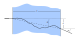
\includegraphics[width=0.9\textwidth]{images/Detector/MultipleScattering.pdf}
    \caption[Schematic View of Multiple Coulomb Scattering]{This is a schematic view of multiple coulomb scattering projected onto a \gls{2d} plane. The solid line is the trace of a particle traversing the detector medium with a thickness $x$, while being deflected by the distance $y$. $\psi$ and $\theta$ denote the deflection angle and scattering angle respectively. This image is sourced from \cite{PDG2018}.}
    \label{fig:MultipleScattering}
\end{figure}
% TODO Maybe move this figure to the end of the paragraph
The \gls{rms} values of these deflection variables in the \gls{2d} plane, $\psi_\text{RMS}$ and $y_\text{RMS}$, are connected to $\theta_\text{RMS}$ and $x$ by \cite{PDG2018}
\begin{align}
    \psi_\text{RMS} &= \frac{1}{\sqrt{3}}\theta_\text{RMS}, \nonumber \\
    y_\text{RMS} &= x \psi_\text{RMS} = \frac{x}{\sqrt{3}}\theta_\text{RMS}.
\end{align}
Since $\theta_\text{RMS}$ is generally rather small, above equation for $y_\text{RMS}$ is simplified, since for small $\theta_\text{RMS}$ we are allowed to replace $\sin{(\theta_\text{RMS})}$ with $\theta_\text{RMS}$. For a momentum measurement in a \gls{lartpc} we observe the random variables within various small columns of \gls{lar} along a particle track. Large deflections are discarded, since they do not contribute to the Gaussian distribution. From this we determine the \gls{rms} variables by a fit over a histogram of the random variables. The column size has to be chosen carefully, because there has to be enough statistics for a $\theta_\text{RMS}$ fit but the column also has to be small enough to avert smearing due to the particle's energy loss. With $\theta_\text{RMS}$ established, it is easy to determine the momentum $p$ by solving equation \ref{eq:MultipleScattering} accordingly. Naturally the multiple scattering method is less accurate than the $\langle -dE/dx \rangle$ measurement. Furthermore, it can not be used for particle identification, since equation \ref{eq:MultipleScattering} only shows a weak particle mass dependence introduced by $\beta$ (consult table \ref{tab:BetheBlochVariables}) which vanishes with high momenta. The MicroBooNE collaboration uses the momentum reconstruction through multiple scattering only for events, whereby the Bragg peak is not contained within the active volume. Given the neutrino beam energy and MicroBooNE's size, these ``uncontained'' tracks are most likely muons.
% TODO ask Davide for the multiple scattering vs. de/dx reconstruction efficiency plots and put it here

A third method to determine a charged particle's momentum could potentially be exploited by the introduction of a strong uniform magnetic field $\vec{B}$ in the active volume. In such a setup, a particle with charge $ze$ and momentum $p = \abs{\vec{p}}$ is subject to the \textbf{Lorentz force} while traversing the magnetic field at a pitch angle $\lambda > \num{0}$. Said pitch angle is defined as the angle between $\vec{p}$ and $\vec{B}$. As the particle looses its momentum in \gls{lar}, its trajectory takes the shape of a spiral with curvature radius $R$ at a given point. In such a case the particle momentum in units of $[\si{\giga\electronvolt}/c]$ is given by \cite{PDG2018}
\begin{equation}
    p = 0.3\, \frac{z R |\vec{B}|}{\cos{(\lambda)}},
\end{equation}
while the units of $|\vec{B}|$ are in $[\si{\tesla}]$ and the units of $R$ in $[\si{\metre}]$. For a momentum measurement in a \gls{lartpc} experiment, one would simply measure the curvature radius $R$ at various points of the track in the upfront calibrated and well known magnetic field. In combination with the outstanding track resolution of a \gls{tpc}, this method would certainly yield the most accurate momentum measurement method, regardless of the track being contained or not. The principle of a working magnetised \gls{lartpc} has already been shown by A. Badertscher \etal \cite{LArTPCMagnetised}, but beyond this small prototype no other experiment has ever used a magnetic field in their active volume. 

In my opinion the persisting reliance on $\langle -dE/dx\rangle$ and $\theta_\text{RMS}$ for momentum measurements marks one of the major shortcomings in our field. We are often blinded by the nice-looking event displays with all their details, forgetting to address the difficulties hidden behind the beauty. The problem could be mitigated by a magnetised \glspl{lartpc}, an idea often proposed, but so far always rejected in the final designs of new detectors. As we reconstruct particle interactions, we eventually rely on hard numbers instead of just beautiful images. Especially for large scale experiments, a magnetised detector should be considered. Unfortunately, magnetised \glspl{lartpc} might not be used in the next generation of large scale detectors.

\section{Energy Dissipation of Neutral Particles} \label{sec:EnergyDissipationNeutral}
Neutral particles, \ie particles without an electric charge, can not be detected directly in a \gls{lartpc}. Their detection depends on a primary interaction which eventually produces charged secondary particles. From these charged secondaries, one tries to reconstruct the neutral particle's energy as well as identifying its flavour. An extreme case of these reconstruction efforts is certainly the neutron, $n$. With a lifetime of ${\tau_n = \SI{880.2(10)}{\second}}$ \cite{PDG2018} it will not decay within a useful time frame for a \gls{lartpc}, since a full \gls{tpc} drift is of the order of milliseconds. Therefore, neutrons can only be detected through spallation events with an argon atom's core, which leave small and localised ionisation spots. Neutron detection, is the major weakness of most noble fluid detectors \cite{NobleGasDetectors}, but there are efforts underway to better reconstruct them. Other neutral hadrons are less problematic, since they decay much faster. The neutral pion $\pi_0$, for instance, features a lifetime of $\tau_{\pi_0} = \SI{8.51(18)e-17}{\second}$ \cite{PDG2018}, after which it most likely decays into two photons. Heavier neutral \glspl{Meson} also feature short lifetimes and decay either into charged particles, lighter neutral \glspl{Meson}, or directly into photons. In the end all neutral \glspl{Meson} eventually leave traces in the detector. Photons, as the force carrier of the \gls{em} force, are a special case and their interaction in \gls{lar} will be described below in more detail.

Of all neutral particles, photons stand out, as they are able to take part in \gls{em} interactions with the detector medium or target material. The photon features three detectable interaction modes in a \gls{lartpc}: \textbf{photoelectric absorption} \cite{PhotoelectricEffect}, \textbf{Compton scattering} \cite{ComptonScattering}, and \textbf{pair production} \cite{PairProduction}, also often referred to as \textbf{photon conversion}. The Feynman diagrams of these processes are depicted in figure \ref{fig:PhotonInteractions}. All three processes are prevalent in different photon energy ranges, depending on the target material. In \gls{lar} the photoelectric absorption is dominant at energies $E \lesssim \SI{0.1}{\mega\electronvolt}$, in the interval $\SI{0.1}{\mega\electronvolt} \lesssim E \lesssim \SI{10}{\mega\electronvolt}$ Compton scattering is prevalent, and at high energies, $E \gtrsim \SI{10}{\mega\electronvolt}$, one finds predominantly pair production (see figure \ref{fig:PhotonAbsorption}). Note, there are two photon interaction channels not listed here, as they are not visible in a \gls{lartpc}. These are: \textbf{photonuclear interactions} \cite{PhotonuclearInteraction} leading to nuclear excitation or fission of heavy elements, if the photon exhibits a respective resonant energy, and \textbf{Rayleigh scattering} \cite{RayleighScattering} which is the elastic form of Compton scattering, \ie the photon does not loose any energy in this process. In the following I will explain the three visible processes with increasing dominance energy.
\begin{figure}[htbp]
    \centering
    \subfloat[Photoelectric Absorption][Photoelectric absorption]
    {
        \fmfframe(10,10)(0,10){\begin{fmfgraph*}(100,50)
            \fmfleft{i1,i2}
            \fmfright{o1,o2}
            \fmf{photon}{i2,v1}
            \fmf{fermion}{i1,v1,v2}
            \fmf{phantom,tension=2}{o1,v2,o2}
            \fmfv{label=$e^-$,label.angle=180,label.dist=0.1cm}{i1}
            \fmfv{label=$\gamma$,label.angle=180,label.dist=0.1cm}{i2}
            \fmfv{label=$e^-$,label.angle=0,label.dist=0.1cm}{v2}
            \fmfv{decor.shape=circle,decor.filled=full,decor.size=1thick}{v1}
        \end{fmfgraph*}}
        \label{fig:PhotoEffect}
    } \hfill
    \subfloat[Compton Scattering][Compton scattering]
    {
        \fmfframe(10,10)(0,10){\begin{fmfgraph*}(100,50)
            \fmfleft{i1,i2}
            \fmfright{o1,o2}
            \fmf{photon}{i2,v1}
            \fmf{photon}{o2,v2}
            \fmf{fermion}{i1,v1,v2,o1}
            \fmfv{label=$\gamma$,label.angle=180,label.dist=0.1cm}{i2}
            \fmfv{label=$e^-$,label.angle=180,label.dist=0.1cm}{i1}
            \fmfv{label=$e^-$,label.angle=0,label.dist=0.1cm}{o1}
            \fmfv{label=$\gamma$,label.angle=0,label.dist=0.1cm}{o2}
            \fmfv{decor.shape=circle,decor.filled=full,decor.size=1thick}{v1}
            \fmfv{decor.shape=circle,decor.filled=full,decor.size=1thick}{v2}
        \end{fmfgraph*}}
        \label{fig:ComptonScattering}
    } \hfill
    \subfloat[Pair Production][Pair production]
    {
        \fmfframe(10,10)(0,10){\begin{fmfgraph*}(100,50)
            \fmfleft{i1,i2}
            \fmfright{o1,o2}
            \fmf{photon,label=$\gamma$,label.side=left,label.dist=0.1cm}{i1,v1}
            \fmf{photon}{i2,v2}
            \fmf{fermion}{o2,v2,v1,o1}
            \fmfv{label=$Z$,label.angle=180,label.dist=0.0cm,decor.shape=circle,decor.filled=30,decor.size=8thick}{i1}
            \fmfv{label=$\gamma$,label.angle=180,label.dist=0.1cm}{i2}
            \fmfv{label=$e^-$,label.angle=0,label.dist=0.1cm}{o1}
            \fmfv{label=$e^+$,label.angle=0,label.dist=0.1cm}{o2}
            \fmfv{decor.shape=circle,decor.filled=full,decor.size=1thick}{v1}
            \fmfv{decor.shape=circle,decor.filled=full,decor.size=1thick}{v2}
        \end{fmfgraph*}}
        \label{fig:PairProduction}
    }
    \caption[Feynman Diagrams of the Photon Interaction Modes]{Shown here are the Feynman diagrams of the three photon interaction modes with the atomic shell of a detector medium. In all three diagrams the incident photon, denoted as $\gamma$, is depicted in the upper left corner. The photoelectric absorption is shown in \subref{fig:PhotoEffect}, Compton scattering in \subref{fig:ComptonScattering}, and pair production in \subref{fig:PairProduction}. The spectator of the pair production process is usually an atomic nucleus and thus depicted above as a grey blob labelled with the atomic number $Z$ of the target atom. Note that the spectator could also be an electron.}
    \label{fig:PhotonInteractions}
\end{figure}
During the photoelectric absorption, shown in figure \ref{fig:PhotoEffect}, the incident photon is absorbed and its full energy transferred to an electron in the atomic shell of the target material. While undergoing Compton scattering, shown in figure \ref{fig:ComptonScattering}, the photon only conveys a part of its energy to a shell electron and thereafter is able to interact further. Usually several Compton scattering processes occur before the photon has lost enough energy and is ultimately absorbed photoelectrically. During pair production, as shown in figure \ref{fig:PairProduction}, the photon is converted into an electron-positron pair, wherefore it has to exhibit an initial energy of at least twice the electron mass, \ie $E_\gamma \geq 2 m_e c^2 = \SI{1.022}{\mega\electronvolt}$. Below said threshold, no conversion can occur. Since pair production by a single photon is violating momentum conservation in some reference frames, a spectator has to present, exchanging an additional photon. The spectator of the pair production process is usually an atomic nucleus, in about \SI{95}{\percent} of the cases in \gls{lar}. In the other $\sim \SI{5}{\percent}$ of the pair production events, the spectator is an electron (see figure \ref{fig:PhotonAbsorption}). As can be seen, eventually every photon is either converted into - or looses its energy to charged particles, which are then detectable in a \gls{lartpc}. 

When considering photon interactions in matter, they are mostly characterised by their intensity as a function of distance travelled in a medium $I(x)$. Said intensity is defined as
\begin{equation} \label{eq:PhotonAttenuation}
    I(x) = I_0 e^{-\mu x},
\end{equation}
with the initial intensity, $I_0$, and the attenuation coefficient, $\mu$, in units of $[\si{\per\centi\metre}]$. The whole term $\exp(-\mu x)$ actually denotes the absorption probability for a single photon. Thus, $I(x)$ of above equation is a statistical distribution and does not determine a single photon's fate, similar to $\langle -dE/dx\rangle$. Furthermore, $\mu$ is actually a function of the photon's initial energy, as shown in figure \ref{fig:PhotonAbsorption}.
\begin{figure}[htbp]
    \centering
    \includegraphics[width=0.9\textwidth]{images/Detector/PhotonAbsorption.pdf}
    \caption[Attenuation Coefficient of Photons in Liquid Argon as a Function of Energy]{Shown here is the attenuation coefficient of photons, $\mu$, in \gls{lar} as a function of photon energy $E$. At energies $E \lesssim \SI{0.1}{\mega\electronvolt}$ the energy dissipation of photons is dominated by photoelectric absorption, in the interval $\SI{0.1}{\mega\electronvolt} \lesssim E \lesssim \SI{10}{\mega\electronvolt}$ by Compton scattering, and at high energies $E \gtrsim \SI{10}{\mega\electronvolt}$ by pair production. For $E \gtrsim \SI{1}{\giga\electronvolt}$, $\mu$ becomes a constant defined by the radiation length, \ie $\mu = 7\rho/(9X_0)$. The data presented in this chart is provided by XCOM \cite{LArPhotonAbsorption}.}
    \label{fig:PhotonAbsorption}
\end{figure}
As can be seen in said graph, the three photon interaction modes contribute in different energy intervals. Furthermore, the \textbf{pair production} is split up into its two components: the interaction in the nuclear field in dark blue and the interaction in the electron field in light blue. In \gls{lar} at photon energies of $E \gtrsim \SI{1}{\giga\electronvolt}$, the absorption coefficient becomes constant and can be written as
\begin{equation}
    \mu(E > \SI{1}{\giga\electronvolt}) = \frac{7}{9}\frac{\rho}{X_0},
\end{equation}
with $\rho$ representing the \gls{lar} density and $X_0$ the radiation length, as previously introduced in equation \ref{eq:Bremsstrahlung}. As a reminder, we defined $X_0$ by the mean distance $X_0/\rho$ over which an electron loses all but $1/e$ of its energy by Bremsstrahlung. Often, the free mean path, $\lambda$, of a photon is used in above considerations instead of $\mu$, it is defined as $\lambda = 1/\mu$. Thus we get the second definition for $X_0$: the distance $X_0/\rho$ represents $7/9$ of the free mean path of pair production by a high energy photon, $\lambda_\text{p.p}$ \cite{PDG2018}. This ought to show how closely related electron and photon interactions are. So how do we actually determine photon energies in a \gls{lartpc}? With the photon absorption, we are again facing random processes, but sometimes they only occur once per photon, unlike ionisation or multiple Coulomb scattering. The solution for this problem is \gls{em} shower reconstruction. 

By now we established that a photon eventually looses its energy to electrons and positrons, through the interaction modes shown in figure \ref{fig:PhotonInteractions}, but the chain of interactions does not end with these secondary particles loosing their energy by ionisation. As shown in section \ref{sec:ParticleInteractions}, especially in figure \ref{fig:BetheBloch}, light particles are dominated by radiative energy losses already at relatively low energies, \ie they exhibit a low critical energy $E_\text{c}$. For electrons and positrons radiative losses are dominant for $E \gtrsim \SI{32}{\mega\electronvolt}$. As the name implies photons are emitted through Bremsstrahlung, during said radiative losses. In the case of the positron, annihilation has to be considered as well, since it is an antimatter particle. The Feynman diagrams of the Bremsstrahlung and electron-positron annihilation \cite{ElectronPositronAnnihilation1,ElectronPositronAnnihilation2} processes are shown in figure \ref{fig:ElectronPositronInteractions}.
\begin{figure}[htbp]
    \centering
    \subfloat[Bremsstrahlung][Bremsstrahlung]
    {
        \fmfframe(10,10)(0,10){\begin{fmfgraph*}(120,60)
            \fmfleft{i1,i2}
            \fmfright{o1,o2}
            \fmf{phantom,tension=2}{i1,v1,i2}
            \fmf{photon}{v2,o2}
            \fmf{fermion}{v1,v2,o1}
            \fmfv{label=$e^\pm$,label.angle=180,label.dist=0.1cm}{v1}
            \fmfv{label=$e^\pm$,label.angle=0,label.dist=0.1cm}{o1}
            \fmfv{label=$\gamma$,label.angle=0,label.dist=0.1cm}{o2}
            \fmfv{decor.shape=circle,decor.filled=full,decor.size=1thick}{v2}
        \end{fmfgraph*}}
        \label{fig:Bremsstrahlung}
    } \qquad \qquad
    \subfloat[Electron-Positron Annihilation][Electron-positron annihilation]
    {
        \fmfframe(10,10)(0,10){\begin{fmfgraph*}(120,60)
            \fmfleft{i1,i2}
            \fmfright{o1,o2}
            \fmf{photon}{v1,o1}
            \fmf{photon}{v2,o2}
            \fmf{fermion}{i1,v1,v2,i2}
            \fmfv{label=$e^-$,label.angle=180,label.dist=0.1cm}{i1}
            \fmfv{label=$e^+$,label.angle=180,label.dist=0.1cm}{i2}
            \fmfv{label=$\gamma$,label.angle=0,label.dist=0.1cm}{o1}
            \fmfv{label=$\gamma$,label.angle=0,label.dist=0.1cm}{o2}
            \fmfv{decor.shape=circle,decor.filled=full,decor.size=1thick}{v1}
            \fmfv{decor.shape=circle,decor.filled=full,decor.size=1thick}{v2}
        \end{fmfgraph*}}
        \label{fig:ElectronPositronAnnihilation}
    }
    \caption[Feynman Diagrams of the Electron and Positron Interaction Modes in an EM Shower]{Shown here are the Feynman diagrams of the electron and positron interaction modes in an \gls{em} shower. An important interaction mode missing here is ionisation, which is depicted in figure \ref{fig:IonisationAndExcitation}.}
    \label{fig:ElectronPositronInteractions}
\end{figure}
Both depicted processes produce at least one additional photon after a mean distance of $X_0/\rho$. This photon will again be able to produce electrons and positrons after a mean distance of $\lambda_\text{p.p} = 9X_0/(7\rho)$, if its energy is high enough. This leads to a cascade of secondary particles called shower. Such an \gls{em} shower could principally be induced by either an electron or a photon as a primary particle.
% TODO Maybe show a picture of a shower in uBooNE
Futhermore, these \gls{em} showers show several useful universal properties, which massively simplify their reconstruction. For instance, there is the \textbf{Moli\`ere radius} $R_\text{m}$ given by \cite{MoliereRadius}
\begin{equation}
    R_\text{m} = X_0 \, \frac{\SI{21.2}{\mega\electronvolt}}{E_\text{c}}.
\end{equation}
It defines the radius of a cylinder along the shower axis within which \SI{90}{\percent} of the initial particle's energy is dissipated. Within a radius of $2R_\text{m}$, \SI{95}{\percent} of the energy is contained. Since the radius of said cylinder is only material dependent and otherwise constant for all energies of the initial shower particle, it becomes obvious that the length of the shower has to exhibit an energy dependence. Said shower length, $X$, is defined by the following relation \cite{ExperimentalTechniques}
\begin{equation}
    X = X_0 \left( \ln{\left(\frac{E}{E_\text{c}}\right)} + C_j \right), \qquad \text{with} \ C_j =
    \begin{cases}
        -1.0 & \text{for} \ j=e^- \\
        -0.5 & \text{for} \ j=\gamma
    \end{cases},
\end{equation}
where $j$ denotes the initial particle flavour inducing the shower. Above equation can thus be used to directly calculate the energy of an initial particle of an \gls{em} shower. However, for any shower energy reconstruction to work, the whole shower has to be contained in the active volume. One question that remains open now is: how do we distinguish the initial particles? The answer is quite simple, it is done through the linear stopping power at the starting point of the shower. If $j = e^-$, we expect a track with a mean length of $X_0$ before the shower starts. On this track we expect $\langle -dE/dx\rangle \approx \langle -dE/dx\rangle_\text{MIP}$. If, however, $j = \gamma$, we expect two tracks and thus a linear stopping power of $\langle -dE/dx\rangle \approx 2 \langle -dE/dx\rangle_\text{MIP}$. This calorimetric discrimination of electron and photon showers marks one of the strengths of the \gls{lartpc} technology, due to its excellent $\langle -dE/dx\rangle_\text{ion}$ and spacial resolutions. An example of said discrimination in a \gls{lartpc} is shown in figure \ref{fig:ElectronPhotonDiscrimination} below.
\begin{figure}[htbp]
    \centering
    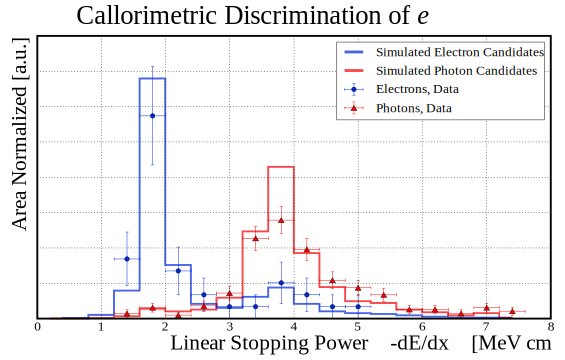
\includegraphics[width=0.8\textwidth]{images/Detector/ElectronPhotonDiscrimination.pdf}
    \caption[Calorimetric Discrimination of Electrons and Photons in a LArTPC]{Calorimetric discrimination of electrons and photons in a \gls{lartpc}, here the results of the ArgoNeuT experiment \cite{LArTPCElectronPhotonDiscrimination}.}
    \label{fig:ElectronPhotonDiscrimination}
\end{figure}
This figure shows a prominent peak at $\langle -dE/dx\rangle = \langle -dE/dx\rangle_\text{MIP}$ for electron induced showers and a slightly broader peak at $\langle -dE/dx\rangle = 2\langle -dE/dx\rangle_\text{MIP}$ for photon induced showers. However, it also becomes apparent that said electron-photon discrimination method is not perfect. It still relies on random processes like the $\langle -dE/dx\rangle$ measurement in a short distance as well as the photon interaction probability $\exp (-\mu x)$. Furthermore, there is the possibility of asymmetric energy allocation to the positron and the electron during pair production. The latter contributes to the broadening of the photon peak to lower $\langle -dE/dx\rangle$. Also, a photon can simply produce a high energy Compton electron creating a \gls{em} shower, which explains the small peak around $\langle -dE/dx\rangle = \langle -dE/dx\rangle_\text{MIP}$ in the photon channel. When the cascade starts to develop in the probing distance of $\langle -dE/dx\rangle_\text{ion}$, higher than expected linear stopping powers are registered.

In the case of MicroBooNE, this excellent calorimetric discrimination between photons and electrons was the main reason for choosing the \gls{lartpc} technology (see MicroBooNE proposals \cite{MicroBooNEProposal1, MicroBooNEProposal2}). The idea being the reduction of the massive \mbox{$\pi_0 \to \gamma + \gamma$} background experienced during MiniBooNE's \gls{lee} measurement. Since MiniBooNE is a Cherenkov detector, it is merely impossible to differentiate between photon and electron induced showers. The reduced background in MicroBooNE is expected to either increase the certainty level of the respective \gls{lee} measurement to $7\sigma$ or reject MiniBooNE's findings.
% TODO Make reference to MiniBooNE result in theory (comming up)

\section{Multiphoton Ionisation by UV-Laser} \label{sec:MultiPhotonIonisation}
A method to ionise \gls{lar} in a controlled manner can be introduced by the use of a coherent beam of photons, a laser. They offer straight ionisation paths with uniform energy deposition along it, creating standard tracks ideal for detector calibration. In principle one could ionise \gls{lar} by a single photon if its energy $h\nu$ equals or exceeds the ionisation potential, \ie $h\nu \geq I_\text{LAr}$. This implies a photon wavelength of $\lambda \geq \SI{92.5}{\nano\metre}$, but lasers emitting these short wavelengths are not available. However, there is a way to ionise \gls{lar} with a laser, namely multiphoton ionisation \cite{MultiphotonProcesses1,MultiphotonProcesses2}. As the name states, the general working principle of this process is the absorption of multiple photons by a single electron in atomic shell, thereby ionising the argon atom. Energy wise all multiphoton ionisation processes feature a single photon energy smaller than the ionisation potential of the medium, \ie $h\nu < I_\text{LAr}$. Nevertheless multiple photons still fulfil the ionisation criterion, \ie $N h\nu \geq I_\text{LAr}$ with the integer $N$ denoting the number of photons. The prove of concept of multiphoton ionisation in \gls{lar} was achieved by J. Sun \etal \cite{LArLaserFirst}. Later our \gls{lar} group at the \gls{lhep} of the University of Bern refined the technology by adding beam energy control, making the technology viable for calibration use cases \cite{LArLaserLHEP}. In the following paragraphs, I will determine the conditions for a multiphoton absorption to occur in \gls{lar}.

We distinguish between three different multiphoton processes: the resonant, the quasi-resonant, and the non-resonant (direct) multiphoton ionisation. In the resonant case the energy of at least one photon equals the energy of a bound excited state with index $i$, \ie $N h\nu = E_i$. These states are relatively long-lived with a lifetime of $\tau_\text{res} \approx \SI{e-8}{s}$ \cite{MultiphotonProcesses1}. However, a purely resonant multiphoton absorption is experimentally hard to achieve, since it would require light beams of different wavelengths to be perfectly aligned and to be fired within the $\tau_\text{res}$ time frame. It thus is favourable to use a single, monochromatic light source. Still, resonant multiphoton absorption plays an important role for most applications, as we will see later.

As their names imply, quasi-resonant and non-resonant multiphoton inonisation occure through virtual states, which are not eigenstates of the atom. In the quasi-resonant case, however, said virtual state is close and slightly above an excited bound state. The non-resonant ionisation does not require any intermediate atomic states. This is possible due to the uncertainty principle first postulated by W. Heisenberg \cite{UncertaintyPrinciple}. In the energy and time realm it can be written as $\Delta E \Delta t \geq \hbar/2$, meaning that the product of the uncertainty in energy $\Delta E$ of an atomic state and the time interval of its existence $\Delta t$ are greater or equal than $\hbar/2$. This relation also defines the lifetime of these virtual states \cite{MultiphotonProcesses1}
\begin{equation} \label{eq:VirtualStateLifetime}
    \tau_\text{virt} = \frac{\hbar}{\Delta E}.
\end{equation}
For the quasi-resonant states $\Delta E$ is directly given by the difference between its energy $E_\text{qr}$ and the next lower atomic state $E_i$, \ie $\Delta E = E_\text{qr} - E_i$. In case of non-resonant states $\Delta E$ is simply the energy difference between the atomic state (mostly the ground state) and the virtual state $\Delta E = N h \nu$. As an example let us consider single photon virtual state ($N=1$) with a wavelength of $\lambda = \SI{266}{\nano\metre}$ exciting a ground state electron to a virtual state. Said virtual state would exhibit a life time of only $\tau_\text{virt} = \SI{1.4e-16}{\second}$, eight orders of magnitude lower than $\tau_\text{res}$. Thus the light source needs to provide a high optical intensity as well as a high level of spacial and temporal coherence in order to induce multiple interactions within this short time frame, properties only found in lasers.

Before we are able to introduce the physical quantities which describe multiphoton processes, we first need to establish some basic formulas of laser physics. For commercially available pulsed lasers key values like pulse width, pulse energy, and wavelength (photon energy) are provided by the manufacturer. From these we can deduce the optical power of a single pulse $P$ as \cite{LaserBasics2}
\begin{equation} \label{eq:PulsePower}
    P = f \frac{E_\text{p}}{\tau_\text{p}},
\end{equation}
where $E_\text{p}$ denotes the pulse energy, $\tau_\text{p}$ the pulse width, and $f$ the pulse shape factor with $f \approx \num{0.94}$ for a Gaussian pulse in time. For reasons of simplification we often consider a Gaussian intensity profile along the beam radius $r$, \ie a so-called \textbf{Gaussian beam}. Thus the intensity is given by \cite{LaserBasics1}
\begin{equation} \label{eq:OptialIntensity}
    I(r) = I_0 e^{-\frac{2r^2}{w^2}}, \quad \text{with} \quad I_0 = \frac{2P}{\pi w^2}.
    % TODO introduce z-dependency with w(z)
\end{equation}
with $w$ standing for the beam diameter, which itself is variable along the beam axis. Using $I_0$ we can calculate the electric field strength amplitude of the laser beam \cite{MultiphotonProcesses2}
\begin{equation} \label{eq:LaserFieldStrength}
    F = \sqrt{\frac{2I_0}{c\epsilon_0\epsilon_\text{r}}}.
\end{equation}

With these quantities established, we are now ready to introduce the main quantity influencing the appearance of multiphoton ionisation, which is the multiphoton ionisation rate per single target molecule, as \cite{MultiphotonProcesses1,MultiphotonProcesses2}
\begin{equation} \label{eq:MultiphotonRate}
    W = \sigma^{(N)} \Phi_\text{ph}^N = \sigma^{(N)} \left(\frac{I}{h\nu} \right)^N.
\end{equation}
Above equation features the generalised cross section of the multiphoton ionisation process $\sigma^{(N)}$ of the $N$\textsuperscript{th} order (units: $[\sigma^{(N)}] = [\si{\centi\metre\tothe{2N}\second\tothe{N-1}}]$), with $N$ again denoting the number of photons necessary to surpass the ionisation potential. Furthermore, we used the photon flux $\Phi_\text{ph}$ given by the intensity of the laser beam $I$ and the single photon energy $h\nu$. Above formula shows the importance of the intensity, since the rate grows with $I^N$. The cross section, though, diminishes rapidly with increasing order, which becomes obvious when considering the process of multiphoton absorption. The first photon excitation to a virtual state features the first order cross section $\sigma^{(1)}$, which has a relatively high value, since there are plenty of stable ground states for a photon to interact with. For the absorption process of a second photon by this first virtual state, the cross section is truncated by the short lifetime and the density of said states in that medium. The two-photon cross section $\sigma^{(2)}$ is therefore the product of $\sigma^{(1)}$ and the cross section of the interaction of a second photon. In summary, it can be stated, that with every additional non-resonant ionisation step, an ever smaller cross section gets multiplied to the previous one, \eg typically resulting in $\sigma^{(1)} \sim \SI{e-17}{\centi\metre\squared}$, $\sigma^{(2)} \sim \SI{e-49}{\centi\metre\tothe{4}\second}$, $\sigma^{(3)} \sim \SI{e-81}{\centi\metre\tothe{4}\second}$, \etc in non-resonant cases \cite{MultiphotonProcesses1}. However, this statement is not valid if resonant states are involved, as is the case in \gls{lar}. For beam intensities higher than \SI{100}{\kilo\watt\per\centi\metre\squared} the ionisation rate of a resonant state is much greater than its decay rate to the ground state, thus greatly increasing $\sigma^{(N)}$ \cite{MultiphotonProcesses1}.

There is, however, another criterion our system needs to fulfil in order to allow the use of the ionisation rate formula in equation \ref{eq:MultiphotonRate}. It is introduced through the adiabatic parameter $\gamma$ for a laser beam in \gls{lar} \cite{MultiphotonCriterion}
\begin{equation}
    \gamma = \omega \frac{\sqrt{2m_eI_\text{LAr}}}{eF}.
\end{equation}
We now can use $\gamma$ to establish the criterion for multiphoton absorption to occur as $\gamma^2 \gg 1$. If $\gamma^2 \ll 1$ the ionisation would be dominated by the tunnel effect, whereby the electron is able to pass through the potential barrier of the atom which is strongly warped by the high electric field strength of the laser beam. When using the values form the first section of table \ref{tab:LaserProperties} for MicroBooNE's laser calibration system as an example, we get $P = \SI{9.4(2)}{\mega\watt}$, $I_0 = \SI{16.6(4)}{\mega\watt\per\centi\metre}$, and thus $F = \SI{91.3(21)}{\kilo\volt\per\centi\metre}$. This results in a $\gamma^2 = \num{5.73e26}$, which clearly meets the condition of $\gamma^2 \gg 1$ and we conclude that typical commercially available lasers are subject to multiphoton absorption in \gls{lar}. In order to be in the realm of tunnel effect dominance, much more powerful lasers would be required than the one of our example.

With an ionisation potential in \gls{lar}, $I_\text{LAr} = \SI{13.4}{\electronvolt}$, and a laser with a wave length of $\lambda = \SI{266}{\nano\metre}$ or a photon energy of $h\nu = \SI{4.66}{\electronvolt}$, a total of three photons are necessary to induce a multiphoton ionisation process, \ie $N = \num{3}$ and thus $Nh\nu = \SI{13.89}{\electronvolt}$. In order to understand the characteristics of this three-photon absorption in \gls{lar} we need to again consider the energy bands of figure \ref{fig:ArEnergyLevelsLiquid}. The first ionisation stage at \SI{4.66}{\electronvolt} is non-resonant, with the aforementioned lifetime of $\tau_\text{virt} = \SI{1.4e-16}{\second}$. The second photon at \SI{9.32}{\electronvolt}, though, seems to fall into several bands and the transition might thus be resonant. But first we have to check if it is an allowed transition. A single photon exhibits two total angular momentum states $J = \pm 1$ given purely by its spin \cite{PDG2018}. Therefore two photons interacting with an single electron are able to change its angular momentum by $\Delta J = -2,0,+2$. Considering argon's ground state with an electron configuration of $1s^2 2s^2 2p^6 3s^2 3p^6$ with $J = 0$ \cite{ArgonEnergyLevels2} and the fact that there are no negative total angular momentum states, it follows that only resonant transition with $J = 0,2$ are allowed. In figure \ref{fig:ArEnergyLevelsLiquid}, the \gls{lar} band structure of excited states with $J = 0,2$ is shown including the three-photon absorption levels. From this we deduce that only two bands are close to the two-photon energy level at \SI{9.32}{\electronvolt}. The first and lower energy state is $1s^2 2s^2 2p^6 3s^2 3p^5\ch{(^2P_{3/2}^o)}4s$ with $J = 2$ \cite{ArgonEnergyLevels2}, which has an upper band boundary of \SI{9.26}{\electronvolt} and thus falls in the quasi-resonant category. This particular quasi-resonant state has a life time of $\tau = \SI{4.3e-13}{\second}$ before decaying into the resonant state. However, since the energy of the third photon still suffices to ionise the atom from said resonant state on, we can consider it as a resonant process for two photons with combined $J = 2$. The band of the second atomic excited state $1s^2 2s^2 2p^6 3s^2 3p^5\ch{(^2P_{1/2}^o)}4s$ with $J = 0$ \cite{ArgonEnergyLevels2} is located between \SIrange{9.28}{9.44}{\electronvolt} and hence is in resonance with a two-photon absorption with a combined angular momentum of $J = 0$. Finally the third and last photon is able to ionise the argon atom in both cases.
\begin{figure}[htbp]
    \centering
    \includegraphics[width=0.6\textwidth]{images/Detector/ArEnergyLevelsLaser.pdf}
    \caption[UV-Laser Induced Three-Photon Ionisation in LAr]{This graph shows the \gls{uv}-laser induced three-photon ionisation process in \gls{lar}. The \gls{uv}-laser in question has a wave length of \SI{266}{\nano\metre} or a photon energy of \SI{4.66}{\nano\metre}, resulting in a three-photon ionisation process with levels at \SIlist{4.66;9.32;13.98}{\electronvolt} drawn in purple. Represented by blue bands are all excited atomic states with a total angular momentum of $J = 0$ and in green the ones with $J=2$ (extracted from figure \ref{fig:ArEnergyLevelsLiquid}). The first ionisation stage is non-resonant, however, the second exhibits a resonance with the band structure of the excited states in \gls{lar} for a combined angular momentum of both photons involved of $J = 0$ ($3p^5\ch{(^2P_{1/2}^o)}4s$), as well as a quasi-resonance for $J = 2$ ($3p^5\ch{(^2P_{3/2}^o)}4s$) \cite{ArgonEnergyLevels2}. From these resonant states the third photon is then able to ionise the excited argon atom by a comfortable margin.}
    \label{fig:ArEnergyLevelsLaser}
\end{figure}

Due to the aforementioned resonance after two photon stages in \gls{lar}, the three-photon ionisation cross section $\sigma^{(3)}$ is a product of the two-photon cross section $\sigma^{(2)}$ and the cross section of a single photon ionising the atom from said bound resonant state $\sigma^{(1)}_{\text{res}}$, \ie $\sigma^{(3)} = \sigma^{(2)} \sigma^{(1)}_{\text{res}}$. The only cross section measurement in \gls{lar}, using the same laser type as MicroBooNE (see section \ref{sec:LaserCalibrationSystem}), was performed by the Argontube group at \gls{lhep} in 2010 \cite{LArLaserCrossSection}. Back then they found that $N = \num{2.02(5)}$ by fitting the three-photon ionisation rate of equation \ref{eq:MultiphotonRate} as a function of photon flux $\Phi_\text{ph}$. This means that the ionisation probability from the resonant state onward is close to one for the laser intensities used in \glspl{lartpc}. Thus our three-photon process of \SI{266}{\nano\metre} photons in \gls{lar} becomes a two-photon process with a cross section measured as \cite{LArLaserCrossSection}
\begin{equation}
    \sigma^{(2)}_{\text{LAr}} = \SI[parse-numbers=false]{\left( 1.24 \pm 0.10_\text{stat} \pm 0.30_\text{syst}\right)\times 10^{-56}}{\centi\metre\tothe{4}\second}.
\end{equation}
Again using MicroBooNE's laser system as an example (see table \ref{tab:LaserProperties}), we get an ionisation rate per argon atom in the laser beam of $W = \SI{6.14e-6}{\per\second}$ resulting in an ionisation yield of roughly \SI{2000}{\per\milli\metre} in the laser track (I checked this number tenfold, cross section is indeed way too low. There is no way this cross section number is supported by the data, must be a calculation error (unit conversion or something)).

% Kerr effect
Another phenomenon influencing the multiphoton ionisation by laser is the Kerr effect. It describes the shift of the refractive index $\Delta n$ of a medium which is subject to high electric fields $E$ \cite{KerrEffect}. Said shift appears due to the induced dielectric polarisation of the material. In static electric fields the effect can be described as
\begin{equation}
    \Delta n = K \lambda E^2,
\end{equation}
with $K$ denoting the material dependent Kerr constant and $\lambda$ the wave length of the refracted light. The Kerr effect can also be induced by dynamic fields, \eg high intensity laser beams with $I > \SI{100}{\kilo\watt\per\centi\metre\squared}$ \cite{KerrEffectLaser}, and is then called \textbf{optically induced Kerr effect}. In this case the shift in refractive index becomes beam intensity dependent and can be approximated by \cite{LaserTheory}
\begin{equation}
    \Delta n \approx n_2 I(r).
\end{equation}
Here, $n_2$ stands for the material dependent nonlinear index of refraction and $I(r)$ for the optical intensity. When considering a idealised laser beam with a Gaussian intensity profile along its radius $r$ (see equation \ref{eq:OptialIntensity}), it follows that $\Delta n$ also exhibits a Gaussian distribution with a maximum on the beam axis. If the optical intensity is high enough, said radial dependency forms a so-called Kerr lens and the beam is subject to self-focusing \cite{LaserBasics2}.

In \gls{lar} this self-focusing of a high intensity laser beam evokes clusters of increased ionisation along the beam axis which are able to saturate or even damage the readout electronics. It creates also massive amounts of space charge leading to field distortions. Self-focusing was observed many times by the Argontube group, although we never further investigated the effect nor published its observation, so it is badly documented in our field. In order to mitigate self-focusing, the beam intensity is reduced by an optical attenuator, which will be discussed later in this chapter (see section \ref{sec:LaserCalibrationSystem}). The goal is to strike a balance between preventing self-focusing and providing enough optical power in order to still induce three-photon ionisation.
% TODO make glossary entries about multiphoton processes and absorption

\section{Recombination and Scintillation} \label{sec:RecombAndScint}
Now let us go back to the detector medium and follow the processes occurring after particle interactions. Immediately after the ionisation and excitation processes in \gls{lar}, see equations \ref{eq:IonisationProcess} and \ref{eq:ExcitationProcess} respectively, we are left with \glspl{quasifreeelectron} $e^-$, argon ions \ce{Ar^+} and argon \textbf{excitons} \ch{Ar^*}. Then, within a time frame of the order of \SI{e-12}{\second}, argon ions undergo \gls{selftrapping} with one of its neighbouring argon atoms, forming charged argon dimers \ch{Ar2^+} \cite{LArSelf-Trapping},
\begin{equation} \label{eq:SelfTrapping}
    \ce{Ar^+ + Ar ->  \ch{Ar2^+}}.
\end{equation}
Some of these charged dimers then recombine with \glspl{quasifreeelectron}. Note, that this recombination process is dependent on the energy deposited in the medium and how much of said energy is transferred to the \glspl{quasifreeelectron}. In the case of multiphoton ionisation by a laser, for instance, recombination can be neglected \cite{LArLaserCrossSection}. In general, the recombination process proceeds in several stages, as described in \cite{NobleGasDetectorsBetter,LArRecombination}. Initially, the dimer is split up again forming a highly excited state \ch{Ar^{**}},
\begin{equation}
    \ce{\ch{Ar2^+} + $e^-$ -> \ch{Ar^{**}} + Ar}.
\end{equation}
Said highly excited state then decays into an argon \textbf{exciton} \ch{Ar^*} in a non-radiative collision process with other argon atoms,
\begin{equation}
    \ce{\ch{Ar^{**}} + Ar -> \ch{Ar^*} + Ar + \text{heat}}.
\end{equation}
Naturally, these excited argon states \ch{Ar^*} are not only produced through recombination alone, but also directly by the incident particles if the transferred energy is too low to overcome the Coulomb-potential of the atom. The latter \ch{Ar^*} production channel was already established in equation \ref{eq:ExcitationProcess}. In dense argon, with number densities $n > \SI{e19}{\per\centi\metre\cubed}$, these \ch{Ar^*} react in a triple collision with two ground state atoms into an excited dimer state, called \glspl{excimer} \cite{LArSelf-Trapping},
\begin{equation} \label{eq:ExcimerProduction}
    \ce{\ch{Ar^*} + 2Ar ->  \ch{Ar2^*} + Ar}.
\end{equation}
Above described production of \ch{Ar2^*} states is achieved by the process of \gls{dynamicaltrapping}, which is estimated to occur within \SI{6e-12}{\second} after the formation of \ch{Ar^*} \cite{LArSelf-Trapping}. Given the number density of \gls{lar} at its \gls{bp}, $n_\text{LAr} = \SI{2.1e22}{\per\centi\metre\cubed}$, and the life time of \ch{Ar^*} in the range of \SIrange{e-9}{e-7}{\second} \cite{NobleGasDetectors}, the vast majority of \textbf{excitons} in a \gls{lartpc} take the form of \glspl{excimer}, \ch{Ar2^*}. It is these \glspl{excimer}, or rather their chemical decomposition, which are responsible for producing a luminescence called \textbf{scintillation light} described by the following process:
\begin{equation}
    \ce{\ch{Ar2^*} ->  2Ar + $\gamma$}.
\end{equation}
This de-excitation marks the end of the recombination process and will be discussed in more detail in the course of this section.

In a \gls{lartpc}, recombination is suppressed by a drift electric field $\vec{E}$ by pulling the two conversely charged ionisation products apart. Thus the more we increase the field strength, $\vert\vec{E}\vert$, the less recombination will occur. In this context, the ratio $Q/Q_0$ is a useful number to quantify recombination or charge reduction processes in general. With $Q_0$ denoting the total electron charge produced during ionisation and $Q$ the charge left charge reduction process, \ie recombination in this case. The breakthrough in quantifying the behaviour of the charge ratio $Q/Q_0$ as a function of electric field came with the theory of G. Jaff\'e \cite{LArRecombinationModel1}. He was the first to realise that recombination has to be treated within the whole charge column of ionisation track and not just as individually insulated electron-ion pairs. The Jaff\'e model results in charge ratio of
\begin{equation} \label{eq:JaffeModel}
    \frac{Q}{Q_0} = \frac{1}{1+q_0 f\left(\vert \vec{E} \vert \sin{(\phi)}\right)},
\end{equation}
where $q_0$ is the initial density of electron-ion pairs and $f$ is a numerically solvable function depending on the projection of electric field strength to the ionisation track direction $\vert \vec{E} \vert \sin(\phi)$, \ie $\phi$ denotes the angle between the ionisation track and the electric field vector. Furthermore, the Jaff\'e model assumes the electrons and ions to be equally mobile, \ie they move with the same velocity when subject to an electric field. As we will see later in this chapter, the latter assumption is wrong. Thus, J. Thomas and D.A. Imel introduced the box model \cite{LArRecombinationModel2}. It is based on the Jaff\'e model, but presumes stationary ions and mobile electrons while disregarding diffusion effects. Then the electron-ion pairs are isolated and uniformly placed in a cubical box as an initial condition. Due to these assumptions the differential equations introduced by Jaff\'e can be solved analytically, which results in
\begin{equation} \label{eq:BoxModel}
    \frac{Q}{Q_0} = \frac{1}{\xi} \ln \left( 1 + \xi \right), \qquad \xi =  \eta \, \frac{Q_0}{\vert\vec{E}\vert},
\end{equation}
with $\eta$ denoting a free parameter used to fit this model to data points. In conclusion, if $\vert\vec{E}\vert \to \infty$, \ie $\xi \to 0$, there will be no recombination, while with $\vert\vec{E}\vert \to 0$, \ie $\xi \to \infty$, all electron-ion pairs recombine. Another way to fit the Jaff\'e model of equation \ref{eq:JaffeModel} directly is given by Birks' law \cite{LArRecombinationModel3}, resulting in
\begin{equation} \label{eq:BirksLaw}
    \frac{Q}{Q_0} = \frac{1}{1+\frac{k_E}{\vert \vec{E} \vert} }.
\end{equation}
Here $k_E$ is the fit parameter. Today, every experiment uses their own adaptations, either of the box model or the Birks' law simplification of the Jaff\'e model in order to fit them to their respective data. The ICARUS collaboration, for instance, used the following adaptation of the Jaff\'e model and Birks' law \cite{LArRecombinationFunction}:
\begin{equation} \label{eq:RecombinationFunction}
    \frac{Q}{Q_0} = \frac{A}{1+\frac{k}{\vert \vec{E} \vert} \frac{1}{\rho} \left\langle -\frac{dE}{dx}\right\rangle}.
\end{equation}
In above equation, $A$ and $k$ are fit parameters and $1/\rho \langle -dE/dx\rangle$ denotes the mass stopping power of the incident particle. Fits performed on ICARUS data suggest the parameters to be $A = \num{0.800(3)}$ and $k = \SI{0.0486(6)}{\gram\kilo\volt\per\centi\metre\cubed\per\mega\electronvolt}$ \cite{LArRecombinationFunction}. The charge ratio according to equation \ref{eq:RecombinationFunction} is shown in figure \ref{fig:Recombination}, for several integer multiples, $N$, of the linear stopping power of a \gls{mip}, \ie $\langle -dE/dx\rangle$ = N $\langle -dE/dx\rangle_\text{MIP}$.
\begin{figure}[htbp]
    \centering
    \includegraphics[width=0.9\textwidth]{images/Detector/Recombination.pdf}
    \caption[Recombination in Liquid Argon]{Depicted here are the recombination curves, $Q/Q_0$ and $L/L_0$, in \gls{lar} as a function of the drift electric field strength $\vert \vec{E} \vert$. They are drawn for five different multiples of the linear stopping power of a \gls{mip}, $N \langle -dE/dx\rangle_{\text{MIP}}$. The dashed lines depicts the fraction of luminosity $L/L_0$ from equation \ref{eq:LuminosityFunction}, and the solid lines the fraction of charge $Q/Q_0$ from equation \ref{eq:RecombinationFunction}.}
    \label{fig:Recombination}
\end{figure}
The charge ratio $Q/Q_0$ is not the only recombination related observable in a \gls{lartpc}, but also the scintillation luminosity ratio $L/L_0$. Here, $L_0$ is defined as the luminosity at $\vert \vec{E} \vert = 0$, \ie the maximum possible luminosity with total recombination. Every luminosity has two components with different origin. One part originates from the excited states, $L_\text{ex}$, produced during ionisation and the other from recombined ionised states, $L_\text{i}$, \ie $L = L_\text{ex} + L_\text{i}(\vert \vec{E} \vert)$. $L_\text{ex}$ is expected to be constant while $L_\text{i}$ is a function of the electric field strength. In fact, when just considering the luminosity stemming from ionisation we can assume,
\begin{equation}
    \frac{L_\text{i}(\vert\vec{E}\vert)}{L_\text{i}(0)} = 1 - \frac{Q}{Q_0},
\end{equation}
with $L_\text{i}(0)$ representing the ionisation luminosity at $\vert\vec{E}\vert = 0$. The relation of the $L_\text{i}(\vert\vec{E}\vert)/L_\text{i}(0)$ ratio to $Q/Q_0$ is a mere logical consequence of recombination, as both are competing for the same electron-ion pairs which either recombine or stay segregated. Combining above assumption together with the definition of $L/L_0$ we get 
\begin{align} \label{eq:LuminosityFunction}
    \frac{L}{L_0} &= \frac{L_\text{i}(\vert\vec{E}\vert) + L_\text{ex}}{L_\text{i}(0) + L_\text{ex}}, \nonumber \\[5pt]
    \Longrightarrow \ \frac{L}{L_0} &= 1 -  \alpha \frac{Q}{Q_0}, \quad \text{with} \quad \alpha = \frac{L_\text{i}(0)}{L_\text{i}(0) + L_\text{ex}}.
\end{align}
This shows how $L/L_0$ and $Q/Q_0$ are intertwined by the recombination process. Furthermore, above derived formula for $L/L_0$ is independent of the respective model used to calculate $Q/Q_0$. The form factor $\alpha$ can be derived from luminosity measurements, which found $\alpha = 0.64$ \cite{LArRecombination} and $\alpha = 0.70$ \cite{LArRecombLuminescence} respectively. Just a quick side note: such discrepancies are common themes of recombination measurements as well as theoretical calculations and should thus be investigated for the use future large scale experiments. The resulting $L/L_0$ function of equation \ref{eq:LuminosityFunction} with $\alpha = 0.70$ is shown for various integer multiples $\langle -dE/dx\rangle_{\text{MIP}}$ as dashed lines in figure \ref{fig:Recombination}. 

As established above, recombined pairs and directly produced \ch{Ar^*} states are mostly transformed into \glspl{excimer} \ch{Ar2^*}. The \glspl{excimer} come in two different energy states: the \gls{singletexcimer} \ce{\ch{Ar2^*}(^{1}\Sigma^+_u)} and the \gls{tripletexcimer} \ce{\ch{Ar2^*}(^{3}\Sigma^+_u)}. Both, the singlet \cite{LArScintillationSpectrum1} and the triplet \cite{LArScintillationProcess1,LArScintillationProcess2}, decay into the same ground state \ce{Ar2(^{1}\Sigma^+_g)} under emission of a photon as follows
\begin{align}\label{eq:Scintillation}
    \ce{\ch{Ar2^*}(^{1}\Sigma^+_u) -> Ar2(^{1}\Sigma^+_g) + $\gamma$}, \\ \nonumber
    \ce{\ch{Ar2^*}(^{3}\Sigma^+_u) -> Ar2(^{1}\Sigma^+_g) + $\gamma$}.
\end{align}
This photon luminescence is termed \textbf{scintillation light}. The likewise resulting ground state of the molecular argon \ce{Ar2(^{1}\Sigma^+_g)} is repulsive, resulting in the immediate dissociation of the \ce{Ar2} molecule into single atoms \cite{NobleGasDetectorsBetter}, 
\begin{equation}
    \ce{Ar2(^{1}\Sigma^+_g) -> 2Ar + \text{heat}}.
\end{equation}
This marks the end of the recombination process, as we are again left with argon atoms at the ground state. The whole cycle, from ionisation of an argon atom to its full recombination back to a ground state described above, is shown in figure \ref{fig:FullRecombinationProcess}.
\begin{figure}[htbp]
    \centering
    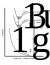
\includegraphics[width=0.7\textwidth]{images/Detector/RecombinationProcessFull.pdf}
    \caption[Full Cycle of the Ionisation/Excitation and Recombination Process]{This figure shows the full cycle of the ionisation/excitation and recombination process. On the $x$-axis we find the nuclear separation a designated argon atom changing its state and a fixed argon atom left at the ground state. The $y$-axis shows the energy of the designated argon atom. (1) indicates the excitation process of our designated atom, \ce{Ar -> \ch{Ar^*}}, after which the resulting exciton is dynamically trapped (2) and forms \ch{Ar2^*} with our fixed atom. (3) is the ionisation process, \ce{Ar -> \ch{Ar^+}} and (4) the rarely occurring direct recombination, \ce{\ch{Ar^+} + $e^-$ -> \ch{Ar^*}}, indicated by the dashed line. In (5) the designated argon ion is self-trapped and forms \ch{Ar2^+} with our fixed argon atom. (6) constitutes the recombination of the self-trapped ion to an \gls{excimer} argon \gls{excimer} \ce{\ch{Ar2^+} + $e^-$ -> \ch{Ar2^*}}. The wavy line denoted by (7), illustrates the scintillation process where the \gls{excimer} decays into its ground state, \ce{$^{1,3}\Sigma^+_{u}$ -> $^1\Sigma^+_{g}$}. Finally, the repulsive ground state $^1\Sigma^+_{g}$ relaxes again into two argon atoms, closing the cycle in (8). Above graph is an adaptation sourced from \cite{LArSelf-Trapping}.}
    \label{fig:FullRecombinationProcess}
\end{figure}

The two photon components emitted in the scintillation processes of equation \ref{eq:Scintillation} are not distinguishable in wavelength and thus the spectrum is characterised by a single peak with a maximum $\lambda_\text{sc} \approx \SI{128}{\nano\metre}$ \cite{LArScintillationSpectrum1,LArScintillationSpectrum2}. A graph of the scintillation spectrum of liquid argon is shown in figure \ref{fig:EmissionSpectrum}.
\begin{figure}[htbp]
    \centering
    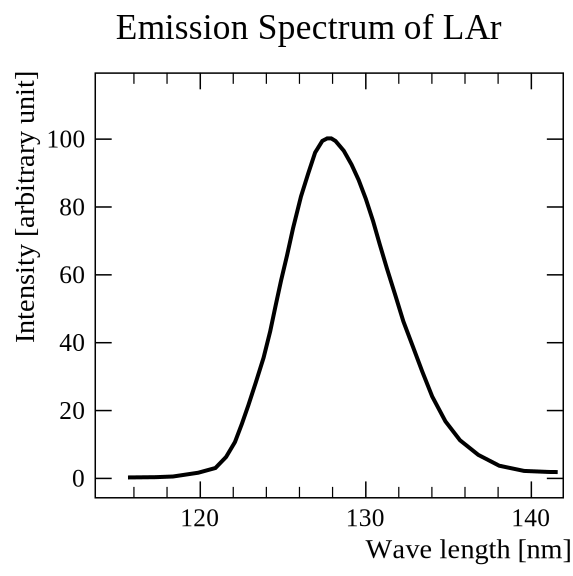
\includegraphics[width=0.7\textwidth]{images/Detector/EmissionSpectrum.pdf}
    \caption[Emission Spectrum of Liquid Argon]{This graph shows the emission (scintillation) spectrum of liquid argon at a temperature of \SI{87}{\kelvin}, redrawn from \cite{LArScintillationSpectrum2}. On the x-axis, the emission wave length is shown while the y-axis represents the intensity in arbitrary units. The spectrum's maximum is around \SI{128}{\nano\metre}.}
    \label{fig:EmissionSpectrum}
\end{figure}
Actually, the direct transition of the triplet state into the ground state \ce{^{3}\Sigma^+_u -> ^{1}\Sigma^+_g} is forbidden, but still occurs, owing to mixing between \ce{^{3}\Sigma^+_u} and \ce{^{1}\Pi_u} through spin-orbital coupling \cite{LArScintillationProcess1}. Thus the decay time of \ce{\ch{Ar2^*}(^{3}\Sigma^+_u)} is much longer, than the one of the \ce{\ch{Ar2^*}(^{1}\Sigma^+_u)} state. For this reason one distinguishes the fast component (\gls{singletexcimer}) with a lifetime of $\tau_\text{s} = \SI{7.0(10)}{\nano\second}$, and the slow component of the scintillation light (\gls{tripletexcimer}) with a lifetime of $\tau_\text{t} = \SI{1.6(1)}{\micro\second}$ \cite{LArScintillationTime}. The ratio of fast and slow component varies with the incident particle type and energy, \ie its linear stopping power; the higher the energy deposited by a particle, the higher the fraction of the fast component \cite{NobleGasDetectorsBetter}. The different scintillation component ratios for \SI{1}{\mega\electronvolt} electrons and \SI{5.4}{\mega\electronvolt} \textalpha-particles are visualised in figure \ref{fig:ScintillationFraction} below. 
\begin{figure}[htbp]
    \centering
    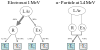
\includegraphics[width=0.8\textwidth]{images/Detector/ScintillationFraction.pdf}
    \caption[Luminosity Ratio of the Slow and Fast Components of Scintillation Light]{This figure shows the different ratios of the fast and slow components of scintillation light in \gls{lar} for \SI{1}{\mega\electronvolt} electrons and \SI{5.4}{\mega\electronvolt} \textalpha-particles. The letter \textbf{R} indicates the recombination origin of the emission, and \textbf{Ex} the exciton origin, respectively. This graph is sourced from \cite{NobleGasDetectorsBetter}.}
    \label{fig:ScintillationFraction}
\end{figure}
The formation of these \ch{Ar2^*} states is incidentally the reason for there being any measurable scintillation light. A decay photon of a simple excited state \ch{Ar^*} would be absorbed through \gls{selfabsorption} and re-emitted multiple times by the dense argon surrounding it (\ce{\ch{Ar^*} <=> Ar + $\gamma$}). Said process is called trapping of resonant radiation and renders the light useless for detection, especially in dense noble liquids. Since there are no naturally occurring ground state \glspl{excimer} \ce{Ar2($^1\Sigma^+_{g}$)} in \gls{lar}, the scintillation light exhibits no resonance to the ground state argon \ce{Ar} surrounding it and is not subject to \gls{selfabsorption}. In other words there is no reverse process to the scintillation light generation of equation \ref{eq:Scintillation}. Hence, \gls{lar} is transparent to its own scintillation light. After its genesis, the scintillation light traverses the \gls{lar} with the speed of light and is eventually either detected by the light readout system (see section \ref{sec:LightReadoutSystems}), or absorbed by other detector structures. Due to its excellent scintillation properties, \gls{lar} is even used in pure scintillation detectors like DEAP-3600 \cite{DEAPExperiment}. \gls{lartpc} experiments like MicroBooNE, however, mostly use the scintillation light as a trigger, \ie to determine the $t_0$ of particle interactions, and do not make use of all the additional information it provides. 

In order to quantify the scintillation light production a W-value, $W_\text{ph}$, is introduced, similar to $W_\text{i}$ in equation \ref{eq:W-ValueDefinition}. $W_\text{ph}$ has also a similar meaning, as it denotes the mean energy an incident particle charged particle, $X^{\pm}$, expends in order to produce a single scintillation photon. The mathematical definition of the W-value for scintillation light is given by
\begin{equation}\label{eq:W-ScintillationDefinition}
    W_\text{ph} \coloneqq k_{\text{i}} I_\text{LAr} + \frac{N_{\text{ex}}}{N}\bar{I}_{\text{ex}} + \bar{\epsilon}_{\text{se}}.
\end{equation}
Note that above equation presumes the production of scintillation light with no electric field applied. In the $W_\text{ph}$ definition we now use the ionisation potential $I_{\text{LAr}}$ and the average excitation potential $\bar{I}_{\text{ex}}$ instead of average expended energy of a particle $\bar{E}_{\text{i}}$ and $\bar{E}_{\text{ex}}$. Further, the form factor $k_{\text{i}}$ is introduced to account for multiply charged and excited charged states, and lastly $\bar{\epsilon}_{\text{se}}$ denotes the average kinetic energy of subexcitation electrons. The later can be understood as the inefficiency of the scintillation light genesis. There are, however, various values of $W_\text{ph}$ for different incident particles and their deposited energy. For heavy relativistic ions $W_\text{ph}$ was measured by T. Doke and K. Masuda \cite{LArWScint-Value1} in \gls{lar} as $W_\text{ph}(\text{max}) = \SI{19.5(10)}{\electronvolt}$. This value also constitutes the maximum yield and is therefore tagged with $\text{max}$. The same physicists also found different values for relativistic electrons close to \gls{mip} energy with $W_\text{ph}(\beta) = W_\text{ph}(\text{MIP}) = \SI{25.1(25)}{\electronvolt}$ and for \textalpha-particles with $W_\text{ph}(\alpha) = \SI{27.5(28)}{\electronvolt}$, respectively. This means that for those two particles the light yield is lower than for heavy relativistic ions. In case of the relativistic electrons the cause for the lower yield is, the low ionisation density along the particle track. This enables some valence electrons to break free from their parent-ions, even without an electric field applied. In other words the electron's thermal energy is higher than the Coulomb potential of the ions and they become so-called \textbf{escape electrons} \cite{LArScintillationEscapeElectron,LArWScint-Value2}. The reason for the lower emission yield of \textalpha-particles lies in the process of \textbf{bi-excitonic quenching}. Said process takes place before the \gls{dynamicaltrapping} of excited states and thus inhibits (quenches) the formation of \ch{Ar2^*} and with it the scintillation light emission. \textbf{Bi-excitonic quenching} is the process of two excited atoms \ch{Ar^*} exchanging the excitation energy while ionising one of them and relaxing the other to its ground state, \ie
\begin{equation}
    \ce{\ch{Ar^*} + \ch{Ar^*} -> Ar + Ar^+ + $e^-$}.
\end{equation}
The excess energy of this reaction is transformed to kinetic energy of the electron, which then becomes an \textbf{escape electron} as described above. This quenching can only occur if the density of excited states \ch{Ar^*} reaches a relatively high level, which is only achieved by incident particles with a high energy transfer to \gls{lar} \cite{LArScintillationQuenching}. Latter is certainly the case for \textalpha-particles, given their relatively high linear stopping power shown in figure \ref{fig:BetheBloch}.

There is also a measurable attenuation of scintillation light due to impurities in the detector medium. It is mainly caused by two impurities in \gls{lar}, \ce{N2} and \ce{O2}, through an additional quenching processes in the early stages of the scintillation light genesis. In the case of \ce{N2} said interference can occur even before the \gls{dynamicaltrapping}, \ie the production of \ch{Ar2^*} (see equation \ref{eq:ExcimerProduction}), can occur. During this quenching, the \ce{N2} molecule collides with the \ch{Ar^*} and the excitation is transmitted \cite{LArScintillationQuenchingN1}, \ie
\begin{equation}
    \ce{\ch{Ar^*} + N2 -> Ar + \ch{N2^*}}.
\end{equation}
Although the excited nitrogen molecule \ch{N2^*} would decay under emission of a photon, it would be in a different wave length and in a different lifetime compared to \ch{Ar2^*} and thus distort the scintillation signature. Above reaction is rather rare at low impurity levels of \si{\ppm} scale, since the \gls{dynamicaltrapping} occurs in a very short time period of \SI{6e-12}{\second}, as established earlier. The quenching takes much longer with $\sim \SI {8e-6}{\second}$ at \SI{1}{\ppm} \cite{LArScintillationQuenchingN2}. Thus the following reactions are dominating the impurity quenching effect for \ce{N2} and \ce{O2},
\begin{align} \label{eq:ScintillationQuenching}
    \ce{\ch{Ar2^*} + N2 -> 2Ar + N2 + \text{heat}}, \\
    \ce{\ch{Ar2^*} + O2 -> 2Ar + O2 + \text{heat}}. \nonumber
\end{align}
Unlike the aforementioned example, these processes are non-radiative, \ie the excitation energy is transformed fully into kinetic energy of the reaction products. As a result, the population of the photon precursors \ch{Ar2^*} is depleted before light emission \ie the emission is quenched \cite{LArScintillationQuenchingN2,LArScintillationQuenchingO2}. The effects of nitrogen and oxygen quenching have been studied extensively, and are found to reduce the scintillation yield by significant quantities at high impurity levels. A \ce{N2} impurity level of \SI{20}{\ppm} was found to reduce the emission intensity by $\sim \SI{60}{\percent}$ \cite{LArScintillationQuenchingN2}, while the same quenching is found at an \ce{O2} level of already \SI{10}{\ppm} \cite{LArScintillationQuenchingO2}. Both impurities show no effect of quenching below a \SI{0.1}{\ppm} concentration. Furthermore, the quenching seems to affect predominantly the slow component of the scintillation light, which means that the impurities predominantly interact with the \gls{tripletexcimer} \ce{\ch{Ar2^*}(^{3}\Sigma^+_u)}. This can be explained by the triplet's much longer lifetime, whereby the impurities have more time to collide with \gls{excimer}. Thus, the impurities have a higher chance of quenching the triplet than the singlet state. In a \gls{lartpc} experiment, \ce{O2} contamination levels are usually mitigated by the use of active copper filters, which are able to bind the oxygen due to its high \gls{electronegativity}. Hence, \ce{O2} contamination does not pose a problem with regards to scintillation light. \ce{N2} levels, on the other hand, are mostly not even measured and, because of the molecules low \gls{electronegativity}, can not be filtered as easily as \ce{O2}. It can be assumed that the \ce{N2} impurity levels would slowly increase in the detector with the passing of time, as a result of small leaks in the cryogenic system, and thus quench emission yields more and more. Thus it is paramount for large scale experiments with long running times to mitigate this problem with molecular sieves or hot metal getters made of titanium or barium. Impurities can also shorten the lifetime of the two \glspl{excimer} along with quenching. It is hypothesised, that soft collisions with impurities may induce an immediate decay \cite{LArScintillationTime}. This shortens the slow component's lifetime $\tau_\text{s}$ in particular, since, again, a longer lifetime increases the chance of a collision.

Recombination and scintillation are studied in much detail, still there are major unknowns for \gls{lartpc} applications; especially in the characteristics of scintillation and its W-value $W_\text{ph}$. Similar to $W_\text{i}$, $W_\text{ph}$ is used in a very liberal way by the neutrino physics community leading to several problems:
\begin{enumerate}
    \item $W_\text{ph}(\text{max}) = \SI{19.5(10)}{\electronvolt}$ is used for all particles, although we are mostly dealing with \glspl{mip} and thus $W_\text{ph}(\text{MIP}) = \SI{25.1(25)}{\electronvolt}$ would probably suit better.
    \item $W_\text{ph}$ has been measured using sources in a limited energy range of the order of \SI{1}{\mega\electronvolt}.
    \item So far $W_\text{ph}$ has not been determined for muons, pions, or protons at all.
    \item The effect of the \gls{lar} density, and thus pressure and temperature, on $W_\text{ph}$ are not measured at all.
\end{enumerate}
The measurements so far were obviously tuned for dark matter research purposes and it is time for the neutrino community to catch-up, even if our needs in regard of scintillation might not be pressing, since it is often only used as a trigger signal. I am certain, that there is a lot of use for a well understood scintillation signal and it could help to achieve more accurate particle identification in \glspl{lartpc}. Therefore a measurement of $W_\text{ph}$ as a function of linear stopping power would be of great value.
% TODO calculate photons per mm with W_ph(MIP)

\section{Charge Carrier Drift} \label{sec:ChargeDrift}
Hitherto we examined rather fast processes occurring in \gls{lar}: the formation of an ionisation track by a charged particle $\mathcal{O}(\SI{e-9}{\second})$, recombination $ < \mathcal{O}(\SI{e-9}{\second})$, \gls{selftrapping} $\mathcal{O}(\SI{e-12}{\second})$, and \gls{excimer} decay, \ie scintillation light genesis, up to $\mathcal{O}(\SI{e-6}{\second})$. Now we will examine the slowest process in a \gls{lartpc}, which is the charge drift. In MicroBooNE sized detectors we observe drift time scales of $\mathcal{O}(\SI{e-3}{\second})$ for \glspl{quasifreeelectron} and $\mathcal{O}(\SI{e3}{\second})$ for ions. \Glspl{quasifreeelectron}, $e^-$, and self-trapped argon ion dimers, \ch{Ar2^+}, which were not experiencing recombination, are then subject to charge carrier drift. In \gls{lar} these point like \glspl{quasifreeelectron} are able to move fast, while the rather large \ch{Ar2^+} ions show an impaired movement behaviour. In addition, these self-trapped dimers are not stable and the charge is able to transfer onto randomly colliding \ce{Ar} atoms which again will be self-trapped. This behaviour screens the charge of the ion, thus increasing its effective mass and further reduces its ability to move also known as \gls{mobility} \cite{NobleGasDetectors}. Note, that the drifting ion species was indeed identified as \ch{Ar2^+} in several measurements \cite{LArMobilityPressure,LArIonDrift1}.

Charge drift is the motion of charge carriers induced by an electric field $\vec{E}$. So in order to achieve a consistent drift, every \gls{tpc}'s field cage is designed in such a way that $\vec{E}$ is as uniform as possible. In case of negatively charged carriers, \eg $e^-$, said motion is vectored against the direction of $\vec{E}$ and thus towards the anode, while positively charged carriers, \eg \ch{Ar2^+}, move with the field vector towards the cathode. The relation between a charge carrier's drift velocity $v_e$ and the electric field strength $E \coloneqq \abs*{\vec{E}}$ is mathematically described as follows \cite{LArElectronDrift1}:
\begin{equation}\label{eq:DriftVelocity}
    v_e(\rho,E) = \mu(\rho,E) E.
\end{equation}
The proportionality function $\mu(\rho,E)$ is called \gls{mobility} and is typically expressed in units of $[\si{\centi\metre\squared\per\second\per\volt}]$ \cite{NobleGasDetectors}. It is a function of $E$ and the drift medium density $\rho$ and thus also dependent on the temperature $T$ \cite{LArMobilityTemperature} and the pressure $p$ \cite{LArMobilityPressure}. A special case of said \gls{mobility} is $\mu_0$ called \gls{zero-fieldmobility} and it is only suitable for small electric field strengths, \ie $\mu = \mu_0$ if $E \to 0$. At these limits it still depends on the medium's density but looses its $E$ dependency. Thus, the drift velocity in equation \ref{eq:DriftVelocity} becomes linear in $E$. In the case of \glspl{quasifreeelectron} in \gls{lar}, the aforementioned linearity and thereby $\mu_0$ are only applicable for $E \lesssim \SI{150}{\volt\per\centi\metre}$, \ie for a rather small range in electric field strength. For a drift electron in \gls{lar} at standard \gls{bp}, the \gls{zero-fieldmobility} is measured as \cite{LArElectronMobility}
\begin{equation} \label{eq:ConstMobility}
    \mu_{0,e} = \SI{516(27)}{\centi\metre\squared\per\second\per\volt}.
\end{equation}
Above \SI{150}{\volt\per\centi\metre}, the electron drift velocity $v_e$ nears and later exceeds the velocity of sound waves (phonons) in \gls{lar} at $c_\text{s} = \SI{842.9(84)}{\metre\per\second}$ \cite{NistChemistryWebBook}. As a consequence the resistance for the drifting electrons in the liquid increases whereby the electron \gls{mobility} $\mu_e$ decreases. Thus the function of $v_e(E)$ flattens with increasing field strength $E$. Heretofore, nobody developed a reliable model of the aforementioned increase in resistance and thus it is best described by an empirical equation \cite{LArElectronDriftFunction}:
\begin{equation}
    v_e(T,E) = \left( 1 + P_1 \left( T - T_0 \right) \right) \left( P_3 E \ln{\left(1+\frac{P_4}{E}\right)} + P_5E^{P_6} \right) + P_2\left( T - T_0 \right).
\end{equation}
The parameters $P_i$ are usually fitted to data points in the region of interest of the corresponding experiment, whereby $T_0$ is set to be the temperature at which the data points were collected. This leads to stitched together functions for $v_e(E)$ when regarding greater intervals in $E$, as is shown in figure \ref{fig:DriftVelocity}. It depicts $v_e(E)$ between \num{0} and \SI{10}{\kilo\volt} at the \gls{bp} temperature $T = \SI{87.303}{\kelvin}$.
\begin{figure}[htbp]
\centering
\includegraphics[width=0.9\textwidth]{images/Detector/DriftVelocityElectron.pdf}     
\caption[Electron Drift Velocity as a Function of Electric Field]{This image depicts the electron drift velocity $v_e$ as a function of electric field strength $E$ from \SIrange{0}{10}{\kilo\volt} at a temperature of $T = \SI{87.303}{\kelvin}$ (\gls{bp} at \SI{1}{\bar}). In the small graph a magnified view of the same drift velocity between \SI{0}{\kilo\volt} and \SI{1}{\kilo\volt} is shown. The function used to draw this graph has three parts. First, from \SIrange{0}{0.15}{\kilo\volt}, the linear function \ref{eq:DriftVelocity} and $\mu_{0,e}$ of equation \ref{eq:ConstMobility} is used. Second, in the range from \SIrange{0.15}{0.7}{\kilo\volt}, an empirical function \cite{LArElectronDriftFunction} with parameters obtained from \cite{LArElectronDrift3} is employed. Third, above \SI{0.7}{\kilo\volt}, the same empirical function is applied with different parametrisation \cite{LArElectronDrift2}. The black vertical line shows the velocity of sound $c_s$.}
\label{fig:DriftVelocity}
\end{figure}
% TODO Draw line where microboone is at!

While drifting, all charge carrier clouds are subject to diffusion, rooted in their Brownian motion. In three dimensions and without an electric field said diffusion is mathematically described by Einstein's abundance distribution \cite{BrownianMotion}
\begin{equation} \label{eq:DiffusionEquationOrigin}
    n(t,\vec{x}) = \frac{N_0}{\left(4 \pi D t \right)^{\frac{3}{2}}} \, e^{-\frac{\vec{x}^2}{4Dt}},
\end{equation} 
with $n(t,\vec{x})$ denoting the number density of the charge carriers at time $t$ and location $\vec{x}$, $N_0$ the total number of charge carriers in the cloud, and $D$ the diffusion coefficient. Above diffusion function will be infinitesimally thin in space at $t=\SI{0}{\second}$ and will spread more with increasing $t$, while its integral remains constant. Therefore, diffusion is observed in a \gls{lartpc} as a spacial spread of the charge signal, widening with drift time. To characterise said spacial spread, the standard deviation $\sigma$ of above distribution is used which is given by \cite{BrownianMotion}
\begin{equation} \label{eq:DiffusionWidthOrigin}
    \sigma = \sqrt{2Dt}.
\end{equation}
The diffusion coefficient $D$ itself is dependent on the energy distribution of the charge carriers. In case of \glspl{quasifreeelectron} in absence of a drift electric field, $D$ is given by the Nernst-Townsent relation for charged particles \cite{LArDiffusionTheory1}
\begin{equation}
    \frac{D}{\mu_0} = \frac{kT}{q},
\end{equation}
with $k$ being the Boltzmann's constant, $T$ the temperature, and $q$ the charge of the particle ($q=e$ in case of $e^-$). The $kT$ part of the equation shows that, in this case, $D$ depends purely on the thermal energy of the charge carrier. It is also interesting to see, how the diffusion coefficient is directly related to the \gls{zero-fieldmobility} $\mu_0$. This makes perfect sense, since it implies that the charge carrier faces the same resistance for Brownian motion and the drift in a weak electric field. In case of electrons, we are able to calculate the diffusion coefficient at standard \gls{bp} and without any drift field as $D = \SI{3.9}{\centi\metre\squared\per\second}$. Applying an electric field also increases the energy of the charge carrier which in turn influences the diffusion coefficient $D$. For electrons, this change is significant and $D$ takes the form \cite{LArDiffusionTheory1,LArDiffusionTheory2}
\begin{equation}
    \frac{D}{\mu} = F \frac{ \bar{\varepsilon}}{e},
\end{equation}
where $\mu$ is now used instead of $\mu_0$ and variable $\bar{\varepsilon}$ denotes the mean electron energy. $F$ is a constant depending on the electron momentum distribution. In case of a Maxwell distribution of electron momenta $F=2/3$ \cite{LArDiffusionTheory1}. The kinetic theories of electrons in \gls{lar}, \ie the derivation of $F$ and $\bar{\varepsilon}$, are by themselves a vast topic and are thus not discussed here. However, I would like to reference the most significant works on this topic by M.H. Cohen and J. Lekner \cite{LArElectronKinematics1,LArElectronKinematics2} as well as V.M. Atrazhev and I.V. Timoshkin \cite{LArDiffusionAnisotropy}. In case of large enough $\bar{\varepsilon}$ the electrons are considered ``hot'' and diffusion looses its isotropy, \ie it becomes directional. It is thus split into two components: the longitudinal component in the $x$-coordinate, parallel to the electric field, governed by $\bar{\varepsilon}_\text{L}$ and its derived diffusion coefficient $D_\text{L}$, and the transverse component in the $y$-$z$-plane perpendicular to the field driven by $\bar{\varepsilon}_\text{T}$ and $D_\text{T}$ \cite{LArDiffusionTheory1,LArDiffusionAnisotropy}. Therefore, let us rewrite the diffusion equation \ref{eq:DiffusionEquationOrigin} as \cite{LArDiffusionTheory1}
\begin{equation} \label{eq:DiffusionEquation}
    n(t,\vec{x}) = \frac{N_0}{4 \pi D_\text{T} t \sqrt{4 \pi D_\text{L} t}} \,e^{-\frac{(x - v_et)^2}{4D_\text{L}t}} e^{-\frac{y^2+z^2}{4D_\text{T}t}},
\end{equation}
where the charge position in the $x$-coordinate now also includes the drift with velocity $v_e$. Above described anisotropy can be subsequently observed in the difference of spacial spread of the charge cloud from equation \ref{eq:DiffusionWidthOrigin} becomes
\begin{equation} \label{eq:DiffusionWidth}
    \sigma_\text{L,T} = \sqrt{\frac{2xD_\text{L,T}}{\mu E}},
\end{equation}
while also converting time $t$ by employing the drift distance $x$, the \gls{mobility} $\mu$, and the electric field strength $E$. Measurements of electron diffusion in \gls{lar} are sparse and often contradicting, see table \ref{tab:Diffusion}.
\begin{table}[hbtp]
    \centering
    \caption[List of Electron Measured Diffusion Coefficients $D_\text{L,T}$ in LAr]{List of measured electron diffusion coefficients $D_\text{L,T}$ in \gls{lar}. There are only a few known measurements of $D_\text{L}$ and some of them seem to differ strongly, although they were measured at similar electric field strengths $E$. For $D_\text{T}$ there is only one known measurement.}
    \begin{tabu} to 0.9\textwidth{cccc} \toprule
        \rowfont[c]{\bf}Measured Coefficient & $\mathbf{E}\ [\si{\volt\per\centi\metre}]$ & $\mathbf{D_{L,T}}\ [\si{\centi\metre\squared\per\second}]$ & Source \\ \midrule
        \multirow{7}{*}{$D_\text{L}$} & \num{0}   & \num{4.5} & \multirow{7}{*}{\cite{LArElectronDiffusionL1}} \\
                               & \num{300} & \num{9.0} & \\
                               & \num{1000} & \num{13} & \\
                               & \num{3000} & \num{18} & \\
                               & \num{1e4} & \num{24} & \\
                               & \num{3e4} & \num{33} & \\
                               & \num{1e5} & \num{34} & \\ \midrule
        \multirow{3}{*}{$D_\text{L}$} & \num{2000} & $\sim \num{3}$ & \multirow{3}{*}{\cite{LArDiffusionTheory2}} \\
                               & $\vdots$ &  $\vdots$ & \\
                               & \num{1e4} & $\sim \num{16}$ & \\ \midrule
        $D_\text{L}$           & \num{100} & \num{4.8(2)} & \cite{LArElectronDiffusionL2} \\ \midrule
        $D_\text{L}$           & \num{120} & \num{5.3(5)} & \cite{Argontube1} \\ \midrule
        $D_\text{T}$           & \num{2700} & \num{15} & \cite{LArElectronDiffusionT} \\ \bottomrule          
    \end{tabu}
    \label{tab:Diffusion}
\end{table}
Considering the most recent theory \cite{LArDiffusionAnisotropy} the longitudinal diffusion component over the full drift length in MicroBooNE is given as $\sigma_\text{L,max} = \SI{1.3}{\milli\metre}$ and the transverse component is expected to be $\sigma_\text{T,max} = \SI{2.0}{\milli\metre}$. The latter can not be observed in MicroBooNE because of its $y$-$z$-resolution of only \SI{3}{\milli\metre}. Hence, diffusion does not interfere with an accurate charge measurement. The effect of diffusion in the MicroBooNE detector over time is shown in figure \ref{fig:Diffusion}.
\begin{figure}[htbp]
\centering
\includegraphics[width=0.9\textwidth]{images/Detector/Diffusion.pdf}     
\caption[Longitudinal Component of the Electron Diffusion Function for Various Drift Times]{Above illustration shows the longitudinal component of the electron diffusion function $n(t,z)/N_0$ (see equation \ref{eq:DiffusionEquation})  with $z = z\prime + v_e*t$ for the drift times \SIlist[list-units = single]{0.05;0.50;2.25}{\milli\second}. The coordinate shift centres all distributions around \SI{0}{\centi\metre} and thus allows for a direct comparison of the $e^-$ distributions. All distributions are calculated using MicroBooNE's operational electric field strength of \SI{273.4}{\volt\per\centi\metre} and the corresponding $\bar{\varepsilon}_{L}$ sourced from \cite{LArDiffusionAnisotropy}. In addition the drift time of \SI{2.25}{\milli\second} corresponds to a full drift from cathode to anode in the MicroBooNE detector during regular operations.}
\label{fig:Diffusion}
\end{figure}

While the charge carriers drift in \gls{lar} they not only undergo diffusion but also collide with impurities. Depending on their \gls{electronegativity}, these impurities are able to capture the charge. This attachment process is predominantly prevalent with \glspl{quasifreeelectron} and can be described as \cite{LArPurity1}
\begin{equation} \label{eq:ImpuitiesGeneral}
    \ce{e^- + S ->[$k_\text{S}$] S^-},
\end{equation}
where \ce{S} is the electronegative impurity molecule and $k_\text{S}$ denotes the rate constant of this process in units of $[\si{\per\mole\per\second}]$. Above process inevitably leads to a reduction of the charge signal in a \gls{tpc}. If the impurities are homogeneously distributed throughout the detector's active volume, said reduction can be described as an exponential attenuation \cite{LArPurity2}
\begin{equation} \label{eq:ChargeAttinuation}
    Q(t) = Q_0 e^{-\frac{t}{\tau}}.
\end{equation}
Here, $Q(t)$ is the amount of \glspl{quasifreeelectron} left after a drift time $t$, $Q_0$ the number of \glspl{quasifreeelectron} right after recombination, and $\tau$ the \textbf{charge lifetime}. The latter is connected to the abovementioned rate constant $k_\text{S}$ \cite{LArPurity3}
\begin{equation} \label{eq:ChargeLifetime}
    \tau = \frac{1}{k_\text{S}n_\text{S}},
\end{equation}
where $n_\text{S}$ denotes the amount of substance \ce{S} in $[\si{\mole}]$. For an accurate charge measurement and reconstruction in a \gls{lartpc} the fraction $Q(t)/Q_0$ needs to be determined, in order to compensate the impurity induced attenuation and reconstruct the ionisation signal. This can be achieved by measuring $Q(t)$ of a constant ionisation source like a \gls{uv}-laser over a variable $t$ \cite{Argontube0} or by determining $Q(t_\text{d})/Q_0$ over a fixed drift time $t_\text{d}$ employing the photoelectric effect \cite{PhotoelectricEffect} of a \gls{uv} flash lamp on the cathode, like in a purity monitor \cite{LArPurityMonitor,LArPurifying}. There are several impurities identified to capture drifting \glspl{quasifreeelectron}, these are: sulphur hexafluoride \ce{SF6}, carbon dioxide \ce{CO2}, nitrous oxide \ce{N2O}, water \ce{H2O}, and oxygen \ce{O2}. Only the latter two, \ce{H2O} and \ce{O2}, are relevant in a \gls{lartpc} as they are the only ones appearing in our atmosphere in considerable amounts. The trapping of \glspl{quasifreeelectron} $e^-$ by most of these impurities, described in equation \ref{eq:ImpuitiesGeneral}, actually occurs in two stages. First, the electron is captured whereby an excited charge state of the impurity is produced. Then, said excited impurity is then relaxed through a collision with a third body, most likely an argon atom \ce{Ar}. The following example shows aforementioned two stage trapping process for an oxygen impurity in \gls{lar} \cite{LArPurity1}:
\begin{align}
    \ce{e^- + O2 &-> \ch{O2^{-*}}} \nonumber \\
    \ce{\ch{O2^{-*}} + Ar &-> \ch{O2^- + Ar^*}}.
\end{align}
All the above impurities exhibit different $k_\text{S}$, which again are $E$ dependent. For MicroBooNE's operating electric field $k_{\ce{O2}} \approx \SI{1e11}{\per\mole\per\second}$, $k_{\ce{H2O}} \approx \SI{8e11}{\per\mole\per\second}$, and the impurity capturing the electrons the strongest $k_{\ce{SF6}} \approx \SI{1.5e14}{\per\mole\per\second}$ \cite{LArPurity1}. In the field of \glspl{lartpc}, oxygen holds a special role in impurity measurements. It serves as a gauge for all electron trapping impurities and thus the term \textbf{oxygen equivalent impurity level} is often used. By doing this, all impurities are assigned the rate constant $k_{\ce{O2}}$ and thus a \ce{H2O} molecule for example would be counted as eight \ce{O2} molecules. In \gls{lar} the oxygen equivalent impurity level, $n_{\ce{O2}}$, is mostly expressed in units of parts per billion $[\si{\ppb}]$ and can be derived adapting equation \ref{eq:ChargeLifetime} as \cite{LArPurity2,LArPurity3}
\begin{equation}
    n_{\ce{O2}} [\si{\ppb}] = \frac{\num{300}}{\tau [\si{\micro\second}]}
\end{equation}
Typical achieved charge lifetimes $\tau$ are of the order of several milliseconds, wherefore oxygen equivalent impurity level $n_{\ce{O2}}$ are usually found in the range from \SIrange{0.3}{0.03}{\ppb}. A stable impurity level can only be achieved by persistent purification. This is attributed to small leaks in the cryo-system and outgassing from built-in components. Said purification is achieved by sintered copper filters and molecular sieves, through which \gls{lar} is circulated by powerful pumps.

% TODO refrase  first sentence
In the case of positively charged argon dimers, \ch{Ar2^+}, the drift velocity is in accordance with the linear function \ref{eq:DriftVelocity}. This time the direction of motion is the same as $\vec{E}$, \ie the opposite direction of the \gls{quasifreeelectron} drift. Since the ion's \gls{mobility} stays constant over a wide range of electric field strength (at least up to \SI{10}{\kilo\volt}) \cite{LArIonDrift2}, there is no need for further complicated empirical equations to describe their movement. The reason for this stability lies in the very slow drift velocity of ions, $v_\text{i}$, which is far below the phonon velocity $c_s$. In fact the \gls{zero-fieldmobility} of argon ions $\mu_{0,\text{i}}$ is six orders of magnitude smaller than $\mu_{0,e}$ and at standard \gls{bp} takes the value of \cite{LArMobilityTemperature}
\begin{equation}
    \mu_{0,\text{i}} = \SI{1.5e-3}{\centi\metre\squared\per\volt\per\second}.
\end{equation}
Using equation \ref{eq:DriftVelocity}, this results in $v_\text{i}$ of the order of \SI{1}{\centi\metre\per\second} in most \gls{lartpc} experiments, which is of the same magnitude as \gls{lar}-flow speeds. At the operational field strength of MicroBooNE, for instance, we find an ion drift velocity of only $v_\text{i} = \SI{0.41}{\centi\metre\per\second}$, which corresponds to a full drift time in excess of roughly \SI{10}{\minute}. Since \ch{Ar2^+} ions dwell for tens of minutes in a \gls{lartpc} the size of MicroBooNE, they are subject to diffusion on a large time scale. Therefore, a large amount of ions is used to measure their mobility. But large amounts of drifting \ch{Ar2^+} themselves contribute significantly to the flow of \gls{lar}, thereby distorting the measurement. Thus, measurements of $\mu_{0,\text{i}}$ show great variations, from \SIrange{0.2e-3}{3.2e-3}{\centi\metre\squared\per\volt\per\second} \cite{LArMobilityPressure,LArIonDrift1,LArMobilityTemperature,LArIonDrift2}. In this work I chose the value that is most applied in the field. Note, that the same value of $\mu_{0,\text{i}}$ is also valid for the impurity ions, like \ch{O2^-} introduced above \cite{LArIonDrift2}. Their movement, however, is directed towards the anode instead of the cathode. Furthermore, I would hypothesise that the drifting argon ions, \ch{Ar2^+}, themselves act as impurities and thus contribute to the \gls{quasifreeelectron} trapping. Since their distribution is not homogeneous throughout the active volume, we have to assume their attenuation function to be more complicated than the one for \glspl{quasifreeelectron} of equation \ref{eq:ChargeAttinuation}. Moreover, the slow drift of the \ch{Ar2^+} ions also contributes to a distortion of the drift electric field of surface detectors. This effect is discussed in more detail in section \ref{sec:SpaceCharge}.

\section{Charge Readout} \label{sec:ChargeReadout}
Arriving at the anode, the clouds of drift electrons are eventually captured by the anode material and can thus be converted to electrical signals. This charge readout process should provide an exact position of the charge on the anode plane, \ie the $y$-$z$-plane. A simple solution for this problem appears to be an array of pixels, which are read out individually. However, this solution scales with $y \cdot z$ and thus generates many readout channels, while a readout channel constitutes the most expensive commodity in every particle detector. Thus, most large scale \glspl{tpc} still use wire plane readouts. Said readouts consist of at least two parallel planes. Within one plane all wires are parallel, but every plane exhibits a different wire angle to one another, \eg see MicroBooNE setup in figure \ref{fig:WirePlaneSetup}. This also provides positional information in $y$ and $z$, although this choice complicates signal reconstruction and introduces some ambiguity when electron clouds arrive at two different spots on the plane at the exact same time. The big advantage of wire plane charge readouts is undoubtedly the reduced scaling of the number of readout channels, from $y \cdot z$ to $y + z$, compared to a pixel array and thus resulting in reduced cost.

Using wire planes without taking additional measures, would result in the \gls{quasifreeelectron} clouds being collected by the first wire plane they encounter, while any plane behind would be shielded completely. In order to achieve the $y$-$z$ position measurement it is paramount to make said first plane transparent to the drift electrons. This is achieved by applying a bias voltage to the wire planes and thus inducing an electric field $\vec{E}_\text{b}$ between them. According to \cite{TPCWireSpacing} transparency of a wire plane is given when
\begin{equation} \label{eq:WireTransparency}
    \frac{E_{\text{b}}}{E_{\text{f}}} > \frac{1+\rho}{1-\rho}, \qquad \text{with} \quad \rho = \frac{2\pi r}{d}. % For microboone the right side rho = pi/10 -> right side = 1.915
\end{equation}
Here the wire plane's back side field strength $E_{\text{b}}\coloneqq \abs*{\vec{E}_\text{b}}$ and the front side field strength $E_{\text{f}}\coloneqq \abs*{\vec{E}_\text{f}}$ need to fulfil above condition. Furthermore, $r$ denotes the wire radius (typically of the order of \SI{100}{\micro\metre}) and $d$ the inter-wire spacing within the plane (typically of the order of \SI{1}{\milli\metre}). In the special case of the first wire plane, $E_{\text{f}}$ equates to the drift electric field strength $E$. The effect of said readout plane transparency on drifting \glspl{quasifreeelectron} is presented in figure \ref{fig:WireTransparency}.
\begin{figure}[htbp]
    \centering
    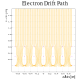
\includegraphics[width=0.6\textwidth]{images/Detector/WireTransparency.pdf}     
    \caption[Electron Drift Paths at the Readout Wire Planes]{The figure presented here depicts a \gls{2d} top view of simulated electron drift paths at the readout wire planes of the MicroBooNE \gls{tpc} \cite{LArTPCReadoutWires}. Shown in purple are the wire cross sections and the drift paths in orange. There are three wire planes: two induction planes on top and at the bottom one collection plane. As can be seen, the electrons circumvent the two induction planes and are collected by the collection plane.}
    \label{fig:WireTransparency}
\end{figure}
Using MicroBooNE's design specifications as an example, the wire plane transparency relation in equation \ref{eq:WireTransparency} is solved to $E_{\text{b}}/E_{\text{f}} > \num{1.92}$. This means that the electric field strength in the back of the induction plane needs to be at least \num{1.92} times larger than the field in the front.

If above transparency relation is satisfied, an approaching electron cloud starts to induce an increasing mirror charge and thus a current in the wires of the first plane. While passing the plane, the mirror charge is reduced and therefore the current reversed. This induction process leads to a bipolar current signal in the transparent plane, hence giving such plane its widely used designation: \gls{InductionPlane}. In order to reduce ambiguities during the reconstruction process, many large detectors like MicroBooNE, make use of two \glspl{InductionPlane}. An example Theoretically there is no limit to the number of induction planes, as long as the condition of equation \ref{eq:WireTransparency} is met. The signal shape of a two induction plane setup is shown in figures \ref{fig:U-PlaneSignal} and \ref{fig:V-PlaneSignal}. At the last plane the a high positive bias voltage is applied which leads to converging field lines onto the single wires (see figure \ref{fig:WireTransparency}). This guides the drift electrons to the wire where they are collected by the wire material. Therefore all experiments use gold coated wires in order to increase collection efficiency. The collected charge leads to a unipolar signal caused by the current of the captured drift electron flowing towards the bias voltage supply. Such collection signals are depicted in figure \ref{fig:Y-PlaneSignal}. Due to the charge collecting nature of the last plane it is called \gls{CollectionPlane}. The \gls{CollectionPlane} signal is the strongest and clearest signal type of a wire plane charge readout system, \ie highest signal-to-noise ratio. Therefore it is considered as the primary signal for event reconstruction and calorimetry. Most shown \gls{2d} event displays in the \gls{lartpc} field are collection plane signals. All charge signals first need to be amplified since they are too weak to process directly, \eg the collected charge of a \gls{CollectionPlane} wire is typically of the order of \SI{1}{\femto\coulomb} \cite{NobleGasDetectors}. The closer this amplification is performed to the readout wire, the better the recorded signal quality, as the noise level increases with conductor length. Nowadays it is standard to use cold amplifiers which are immersed in \gls{lar} and can be mounted directly at the end of the charge readout wire.

In my opinion, the future of \gls{lartpc} charge readout systems are pixelated solutions. First demonstrations of this technology were recently performed by the liquid argon group at \gls{lhep} at the University of Bern \cite{LArTPCReadoutPixels}. Then, apart from difficulties with event reconstruction, wire plane readouts exhibit relatively high noise levels compared to pixels. The main contributor in this regard are the wires themselves which act as perfect antennas for \gls{em} background. Another drawback is introduced by the bias voltage in order to achieve wire plane transparency. For this the signal path needs to be decoupled from the wire by a capacitor, which further worsens the noise situation. There are mechanical challenges too, since the wires must not touch each other, especially the ones from different planes because they would short the bias voltage supply. Thus engineers need to conceive elaborate tensioning systems and work with tight tolerances while producing the wire planes. All these challenges could be avoided by simply using a single pixel array which only works as a \gls{CollectionPlane}. With the dawn of new technologies like cold amplifiers and modern readout electronics becoming lower priced, the pixel readout plane will certainly be the charge readout of choice of future \glspl{lartpc}. This will also bring a direly needed boost in reconstruction accuracy.
\begin{figure}[htbp]
    \centering
    \subfloat[U-Plane Signal][U-plane induction signal]
    {
        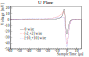
\includegraphics[width=0.5\textwidth]{images/Detector/WireSignalUPlane.pdf}
        \label{fig:U-PlaneSignal}
    } %\qquad
    \subfloat[V-Plane Signal][V-plane induction signal]
    {
        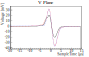
\includegraphics[width=0.5\textwidth]{images/Detector/WireSignalVPlane.pdf}
        \label{fig:V-PlaneSignal}
    }
    \\
    \subfloat[Y-Plane Signal][Y-plane collection signal]
    {
        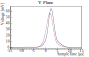
\includegraphics[width=0.5\textwidth]{images/Detector/WireSignalYPlane.pdf}
        \label{fig:Y-PlaneSignal}
    }
    \caption[Typical Wire Signal Wave Forms in a LArTPC]{This figure shows typical wire signal wave forms of a \gls{lartpc}. The wave forms presented above arise from the same MicroBooNE electron path simulation \cite{LArTPCReadoutWires} as introduced in figure \ref{fig:WireTransparency}. Here, the U-plane \subref{fig:U-PlaneSignal} denotes the first, and the V-plane \subref{fig:V-PlaneSignal} the second induction plane, while the Y-Plane \subref{fig:Y-PlaneSignal} is the collection plane. The black line designated ``\num{0} wire'' depicts the signal for charge drifting within one half pitch distance of a central wire. The coloured lines labelled by ``$[-N,+N]$ wire'' show the wave form on a central wire of longer charge tracks with a length of $N$ wire pitches on each side of the central wire. All tracks are parallel to the readout planes as well as horizontal to the earths surface.}
    \label{fig:WireSignals}
\end{figure}

%--------------------------------------------------------------------------------------------------------------------------
% \section{Adverse Effects of the Slow Drift}
\section{Light Readout Systems} \label{sec:LightReadoutSystems}
The goal of a light readout system is to convert in \gls{lar} produced scintillation light into an electric signal which provides intensity and time information. Therefore scintillation photons first need to be converted into electrons by the photoelectric effect. These electrons then need to be multiplied in a controlled manner and thereafter captured in order to induce a voltage. Finally, said voltage is amplified and digitised. The photon conversion and electron multiplication is achieved using \acrfullpl{pmt} or \glspl{sipm}.

A \gls{pmt} consists of a series of dynodes in vacuum tube made of glass. On the tube's top, one finds the photocathode which is usually just a glass surface metallised from the inside. On its bottom a \gls{pmt} features several electric contacts for the voltage supply of the dynodes as well as the signal readout. The photocathode is supplied by a bias voltage, usually between \SIrange{-0.5}{-2.5}{\kilo\volt}. A voltage divider then steps down the voltage for each dynode until the signal is read out at the ground dynode. \Glspl{pmt} can also be operated by connecting the cathode to ground and step up a positive voltage on the dynodes. In said case, a \gls{pmt} is operated in reverse bias mode. Whichever operation mode is chosen, the working principle stays the same: First a photon hits the photocathode and produces a \gls{pe} through the photoelectric effect. Accelerated by the electric field between the cathode and the first dynode, the electron, when hitting the dynode, produces secondary emission, \ie the impact of one high energy electron leads to the emission multiple electrons with lower energies. These secondary electrons are now again accelerated between the first and second dynode each again inducing secondary emission at the latter. This multiplication repeats itself after every dynode gap and results in electron gains of up to \num{e9}. The signal is prompt with rise times of about \SI{2}{\nano\second} and the event frequency can reach a couple of \SI{100}{\mega\hertz}. The concept of the \gls{pmt} was developed by H. Iams and B. Salzberg \cite{PMTFirst}.

The \gls{sipm} is a silicon chip with multiple independent pixels. Each pixel contains a p-n junction which is operated in Geiger-mode \cite{SiPMFirst}, \ie the junction is operated above its breakdown voltage. A breakdown in silicon is defined as electrons and holes gaining enough energy to create new electron hole pairs leading to an avalanche. If a photon now hits a pixel cell the breakdown is triggered within it, leading to gains up to \num{e6} \cite{SiPMReview}. The breakdown is quenched by high-ohmic resistors between the chip and the power supply, temporarily reducing the bias voltage across the p-n junction. Since the breakdown in a single cell always has the same characteristics independent of the amount of photons triggering it, the light intensity has to be measured by the amount of pixels producing a signal. Furthermore, the pixels are not read out individually, but the whole chip produces a signal according to the sum of all pixel signals. The operation in Geiger-mode also leads to spontaneous breakdowns constituting the so-called dark rate of a \gls{sipm} chip given by roughly $\SI{1}{\mega\hertz\per\milli\metre\squared}$ \cite{SiPMReview}. This dark rate can be significantly reduced by requiring a signal from multiple pixels, rather than from a single one.

As established before, scintillation light is emitted at \SI{128}{\nano\metre} wavelength. This poses a problem for a \gls{pmt}, because its photocathode is inside of the \gls{pmt}'s glass surface and glass is an excellent \gls{uv} light absorber. Thus wavelength shifting materials are used in \gls{lar} detectors in order to convert the \SI{128}{\nano\metre} \gls{uv} light into the visible range of the spectrum. The wavelength shifter most used in \glspl{lartpc} is \gls{tpb} \cite{TPB1,TPB2} an organic fluorescent substance able to convert \gls{uv} into visible light within picoseconds \cite{TPBTiming}. The emission spectrum of \gls{tpb} ranges from \SIrange{400}{525}{\nano\metre} (blue to green light) with a main peak at \SI{425(20)}{\nano\metre} \cite{TPBSpectrum}. \Gls{tpb} coatings are either applied directly to the glass surface of the \gls{pmt} or to a transparent (acrylic) shield in front of it. A major issue with \gls{tpb} is attributed to its degradation into benzophenone under \gls{uv} light exposure \cite{TPBDegradation}. Even worse, benzophenone is an commercially produced \gls{uv} blocker. Since benzophenone features an additional oxygen atom in its chemical structure compared to \gls{tpb}, said degradation only applies in oxygen rich environments. So, it can be assumed that principally the degradation of \gls{tpb} in ultra pure \gls{lar} should be of little relevance. However, most recent studies showed that \gls{tpb} emanates from the coatings into \gls{lar}, which could lead to a degradation of the light signal \cite{TPBDissolving}. Therefore, the community tries to find better solution than the \gls{tpb} - \gls{pmt} combination.

\glspl{sipm}, on the other hand, technically do not need a wavelength shifter, since they are not covered by an \gls{uv}-absorbent material. Short wavelengths are even advantageous as they also feature shorter absorption-lengths in silicon \cite{SiPMMasterBaeschu}. The disadvantage for a direct use is their size with only several square millimetre of active area. Still, \gls{sipm} based light readout systems are considered the future in the \gls{lartpc} community, since they provide better light intensity resolution and lower cost. In modern detectors a transparent polymer plate coated with dichroic reflectors and wavelength shifting materials are used as light traps in order to guide the light to an array of \glspl{sipm} \cite{SiPMLArTPC}. Although still not reaching the photon detection efficiency of a \gls{pmt}, such a light detection system is easily scalable and can thus partially compensate its deficiency by a larger area. MicroBooNE opted for the classical \gls{tpb}, \gls{pmt} approach, as the \gls{sipm} technology had not been tested in \gls{lar} at the date of the experiments conception.
% TODO Put this below recombination and scintillation chapter?
% TODO Maybe produce drawing of PMT and SiPM side by side?

\section{Electric Field Generation} \label{sec:LArElectricField}
In order to generate a uniform electric field in a \gls{tpc}, the supply of \gls{hv} to the cathode is essential and still poses a major limitation to \gls{tpc} sizes today. There are two methods employed to supply \gls{hv} to a \gls{lartpc}. The most common one provides the voltage directly from a \gls{dc} power supply to the cathode using a feedthrough to enter the cryostat. Resistors, typically of the order of \SI{100}{\mega\ohm}, between the field cage rings provide a regular step down of the voltage. Every resistor has the same resistance $R$ forming a so-called voltage divider circuit. This resistor chain is connected to ground at the anode. The described assembly provides a uniform electric field and is illustrated in figure \ref{fig:VoltageDivider}. Another, more exotic method is the \gls{hv} generation inside the cryostat employing a Cockcroft-Walton multiplier circuit fed by a lower voltage \gls{ac} power supply, typically several kilo volts. The Cockcroft-Walton circuit uses two chains of capacitors with a constant capacitance $C$ and one interlinked chain of diodes to pump electrons up the diode stages thus continuously multiplying the peak-to-peak input voltage by the stage number. Theoretically every stage can be connected to a field cage ring to achieve a regular voltage increase, see figure \ref{fig:CockcroftWalton}.
\begin{figure}[htbp]
    \centering
    \subfloat[Voltage Divider][Voltage divider circuit with \gls{dc} voltage supply]
    {
        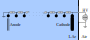
\includegraphics[width=0.7\textwidth]{images/Detector/TPCVoltageSupplyDC.pdf}
        \label{fig:VoltageDivider}
    }
    \\
    \subfloat[Cockcroft-Walton][Cockcroft-Walton multiplier circuit with \gls{ac} voltage supply]
    {
        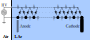
\includegraphics[width=0.7\textwidth]{images/Detector/TPCVoltageSupplyAC.pdf}
        \label{fig:CockcroftWalton}
    }
    \caption[TPC Field Cage Voltage Supply Methods]{Above figures show the two voltage supply methods for the field cage of a \gls{lartpc}. The field cage rings are depicted as filled black circles. In \subref{fig:VoltageDivider} the classical voltage divider is illustrated, with a resistor chain, connecting the field cage. In \subref{fig:CockcroftWalton} the complex circuit of the Cockcroft-Walton multiplier is shown, with ever multiplier stage connecting to a field cage ring.}
    \label{fig:FieldCageVoltageSupply}
\end{figure}
The \gls{dc} supply and resistor chain method has the advantage that they can be easily gauged to provide a very uniform field. With increasing detector size, however, it becomes very hard to construct a feedthrough which is able to handle the increased \gls{hv} and the temperature gradient from room temperature outside of the cryostat to \SI{87}{\kelvin} when immersed in \gls{lar}. For all high voltage feedthroughs a coaxial design is adopted with an inner \gls{hv} conductor, surrounded by an insulator, within a ground shield. At the lower part of the feedthrough the ground shield is curved away and the now bare insulator is ripped to increase the surface distance between conductor and ground shield. The best performing feedthrough so far was able to stably hold \SI{-130}{\kilo\volt} in purified \gls{lar}, employing \gls{petc} as an excellent insulator material \cite{LArBreakdownNew2}. The \gls{ac} supply and Cockcroft-Walton method is advantageous on the feedthrough side, since only a fraction of the voltage has to be supplied, usually several kilovolt. Feedthroughs rated for several kilovolt can be purchase from various suppliers and feedthrough breakdowns are not an issue. The disadvantage, however, is the electric field non-uniformity which is rooted in the undercharging of the circuit. To fully charge the circuit, it would take an infinite amount of time. Moreover, leak currents through the back direction of the diodes exacerbate the undercharging. The more Cockcroft-Walton stages there are, the worse the non-uniformity of the voltage supplied to the field cage rings and thus the drift electric field \cite{Argontube3}. 

Another challenge is to hold the \gls{hv} on the cathode without an electric breakdown, which is able to destroy sensitive electronics. The latter issue is especially prevalent in the gap between a \gls{tpc}'s cathode at voltages of the order of \SI{100}{\kilo\volt} and the grounded cryostat. For a long time \gls{lartpc} community considered the \gls{DielectricStrength} of \gls{lar} to be the universal limit for all \glspl{lartpc}. Said \gls{DielectricStrength} was measured by D.W. Swan and T.J. Lewis around 1960 in a range from \SIrange{1.1}{1.4}{\mega\volt\per\centi\metre} \cite{LArBreakdownOld1,LArBreakdownOld2}. Consequently the community's rule for the allowed maximum electric field strength in \gls{lar} was claimed to be $E_\text{max} < \SI{1}{\mega\volt\per\centi\metre}$. However, while \glspl{lartpc} operate with gap distances between cathode and ground of the order of \SIrange{1}{10}{\centi\metre} and oxygen equivalent impurity levels of \SIrange{0.01}{1}{\ppb}, Swan's and Lewis' experimental setup exhibited gaps between \SIrange{1}{100}{\micro\metre}, impurity levels around \SI{0.2}{\ppm}, and comparably small surfaces. Therefore, Swan's and Lewis' value are not valid for \gls{lartpc} experiments. The first large scale \gls{lartpc} experiment ICARUS T600 \cite{ICARUST600}, designed with at least ten times lower electric fields than above condition, seemed to miss their initial design cathode voltage. It was thought that the issues were only related to the feedthrough design and thus later experiments like ARGONTUBE \cite{Argontube0,Argontube2} and ArDM \cite{ArDM} used Cockcroft-Walton circuits to generate \gls{hv} within the \gls{lar}. ARGONTUBE with a maximum design field of $E_\text{max} = \SI{187}{\kilo\volt}$ was specified way below the \SI{1}{\mega\volt\per\centi\metre} limit and still missed its design cathode voltage by about a factor of 1/4 (design \SI{500}{\kilo\volt}, reached \SI{120}{\kilo\volt}) \cite{Argontube2}. 

While ICARUS and ArDM never addressed their \gls{hv} problems, but rather adjusted their detector specifications, we, the ARGONTUBE group at \gls{lhep} further investigated this issue. In a dedicated measurement, electric breakdowns were observed down to a field strength of $E = \SI{40}{\kilo\volt\per\centi\metre}$ at an impurity level of \SI{1}{ppb} and a gap distance of the order of $\SI{1}{\centi\metre}$ \cite{LArBreakdownNew1}. For increased impurity levels the stable electric field was found to be higher. Also, in this work we attributed this low value to a mechanism similar to the \textbf{Malter effect} \cite{MalterEffect} which describes the increase in electron emission from a cathode covered in a thin insulating layer due to the presence of space charge. In earlier works it was observed that noble gas atoms form atomic monolayers around metals through attractive \glspl{VanDerWaalsForce} \cite{LArMonolayer1,LArMonolayer2,LArMonolayer3,LArMonolayer4}. In a \gls{lartpc}, the argon atoms from a crystalline monolayer around the negatively charged cathode and thus create a thin dielectric barrier on the cathode's surface. When applying the cathode voltage in a \gls{lartpc}, space charge consisting of positively charged argon dimers \ch{Ar2^+} and \gls{quasifreeelectron} form not only in the active volume but also between the cryostat walls and the cathode. As the ions drift towards the cathode, their recombination at the cathode's surface is impeded by the crystalline monolayer, which leads to steep electric field gradients between the cathode and the surrounding space charge clouds. As a consequence the cathode's \gls{WorkFunction} is reduced and discharges develop more easily. In figure \ref{fig:MalterEffect} the above described situation is depicted in a schematic manner.
\begin{figure}[htbp]
    \centering
    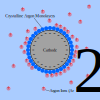
\includegraphics[width=0.5\textwidth]{images/Detector/MalterEffect.pdf}     
    \caption[Malter Effect in Liquid Argon]{A schematic view of the monolayers of crystalline argon a cathode spherical cathode. Attracted by \gls{VanDerWaalsForce}, \ce{Ar} atoms (blue) form an atomic monolayer around metal surfaces, in this case the cathode surface. The negative charge of the cathode attracts \ch{Ar2^+} ions and the monolayer impedes the recombination of the ions with electrons on the cathode surface. Thus, a steep electric field gradient is induced which in turn may trigger an electrical breakdown of the cathode, similar to the Malter effect \cite{MalterEffect}.}
\label{fig:MalterEffect}
\end{figure}
A later study by \gls{fnal} showed a cathode shape dependence of discharge probabilities \cite{LArBreakdownNewFNAL}. In general discharges are a stochastic process and thus the chain of events leading to them is not repeatable, but there still is a general rule for the circumstances they develop. Aforementioned rule predicts the electric breakdown field between the cathode and the ground $E_\text{max}$ as a function of the stressed cathode area $A$ where the electric field exceeds \SI{90}{\percent} of $E_\text{max}$ \cite{LArBreakdownFormula}:
\begin{equation}\label{eq:LArBreakdownFunction}
    E_{\text{max}} = CA^p.
\end{equation}
The constants $C$ and $p$ are used as fit parameters. A combined fit of \gls{lar} breakdown experiments performed at \gls{lhep} \cite{LArBreakdownNew2,LArBreakdownNew1} and \gls{fnal} \cite{LArBreakdownNewFNAL} resulted in $C = \SI{139(5)}{\kilo\volt\per\centi\metre\tothe{3p}}$ and $p=\num{-0.22(1)}$. Said fit of above function and the $E_\text{max}$ measurements cited before are illustrated in figure \ref{fig:LArBreakdownFunction}. As one can see, the data points are broadly scattered around the fit function. The latter acts as a mean and not a limit, \ie if one wants to operate a \gls{lartpc} without discharges, the corresponding $E_\text{max}$ of the fit must be reduced by at least a factor of two.
\begin{figure}[htbp]
    \centering
    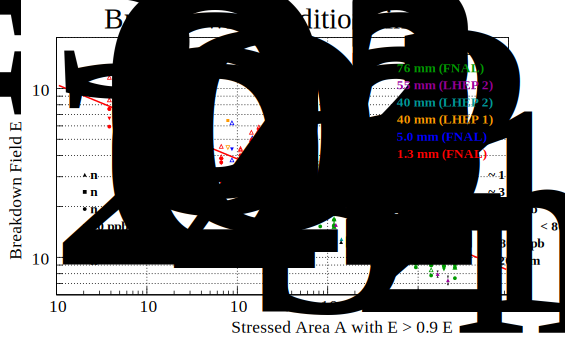
\includegraphics[width=0.9\textwidth]{images/Detector/LArBreakdownFunction.pdf}     
    \caption[Breakdown Field in Liquid Argon as a Function of Stressed Cathode Area]{Breakdown field $E_\text{max}$ as a function of stressed cathode area $A$ with $E > 0.9 E_\text{max}$. The shape of the data points corresponds to different oxygen equivalent impurity levels $n_{O_{2}}$, while the different colours stand for cathode radii used in various experiments. All data points are sourced from three publications: (FNAL) \cite{LArBreakdownNewFNAL}, (LHEP 1) \cite{LArBreakdownNew1} and (LHEP 2) \cite{LArBreakdownNew2}. The red line represents the best fit for equation \ref{eq:LArBreakdownFunction} with parameters $C = \SI{139(5)}{\kilo\volt\per\centi\metre\tothe{3p}}$ and $p = \num{-0.22(1)}$. This illustration is an adapted version sourced from \cite{LArBreakdownNew2}.}
\label{fig:LArBreakdownFunction}
\end{figure}

After the first measurement at \gls{lhep}, we still had questions on how breakdowns actually form. In a second measurement campaign we therefore employed a highspeed camera and an optical spectrometer to analyse the process of the discharge itself \cite{LArBreakdownNew2}. In this study we could identify the three stages of an electrical breakdown in \gls{lar}. The first phase starts with the field emission of electrons from a point on the cathode. Said electrons drift towards the ground, ionising and exciting argon atoms on their way. This process features a visible cone developing between the starting point on the cathode and the ground plate. The cone emits a broad spectrum of light centred around \SI{580}{\nano\metre} (yellow colour). While developing the brightness of the cone increases exponentially, a signature of an avalanche ionisation. Now the produced argon ions drift towards and converge onto the field emission point on the cathode, heating the area significantly above the \gls{bp}. About \SI{2}{\milli\second} after the beginning of the first phase, this occurrence leads to the creation of an argon gas bubble on the cathode surface and thus to the initiation of the second phase. Since argon gas is a better conductor and features a higher avalanche multiplication factor than \gls{lar}, a plasma forms in the bubble. The plasma formation now shields the field emission at the cathode and the cone is quenched. Accelerated electrons in the plasma hit the gas-liquid interface of the bubble causing it to grow and elongate. This formation is called a streamer. Its tip advances on a rambling path in the general direction of the field lines at a velocity of $\sim \SI{300}{\milli\metre\per\second}$. This leads to the growth of a thin and ever longer filament. The streamer has a sharp peak at \SI{700}{\nano\metre} (red) in its emission spectrum, while the advancing tip emits white light (broad spectrum). When the streamer hits the ground plate it establishes a highly conductive channel between cathode and ground. This initiates phase three: the electrical breakdown of the cathode through a spark discharge. The third phase is characterised by a short bright flash, an acoustic shock, and subsequently by intensive bubble formation. The emission spectrum of the breakdown is continuous and dominated by blue and green emissions. The above process can be observed in two videos of breakdowns in \gls{lar} taken at a shutter speed of \SI{1250}{\fps} which are published as data supplements\footnote{\url{http://stacks.iop.org/jinst/11/P03017/mmedia}} of our paper \cite{LArBreakdownNew2}.

For large scale \glspl{lartpc}, with drift lengths of the order of \SI{10}{\metre}, the above discussed breakdown mechanisms poses a major challenge since they will feature cathode voltages of the order of \SI{1}{\mega\volt}. This means that they will feature cathode to ground gaps of the order of \SI{1}{\metre}, leading to a huge unused volumes of \gls{lar}. However, there is a way to increase the breakdown field by coating the cathode in a thin layer of polyisoprene (latex rubber), as discussed in a third \gls{hv} paper from our group \cite{LArBreakdownSuppression}. We measured an electric breakdown filed strength $E_\text{max} = \SI{412}{\kilo\volt\per\centi\metre}$ after applying a layer of \SI{450}{\micro\metre} of polyisoprene. This corresponds to more than a tenfold increase of $E_\text{max}$ compared to a bare metal cathode. This is attributed to the low electron mobility of polyisoprene in the range between \SIrange{e-11}{e-4}{\centi\metre\squared\per\volt\per\second}. This causes the electrons to slowly drift through the material, thus inhibiting the avalanche formation. At the polyisoprene-\gls{lar} interface they recombine with the \ch{Ar2^+} ions, since the crystalline monolayer is only formed on metal surfaces and is thus not present in this setup. This could be the solution for the \gls{hv} problem of \glspl{lartpc}, although after a single breakdown such a coating looses its discharge quenching property.

It took decades until the breakdown issue was acknowledged which I personally attribute to a general shyness and maybe a grain of false pride in our community. It was seen as a failure, if the own experiment could not reach the specified voltages. Therefore, these ``failures'' were not mentioned in publications. Only when meeting people in person at conferences, one was able to share the issues experienced. Still I think the \gls{hv} breakdown investigations were finally a good example of how the \gls{lartpc} community should investigate problems in the field. People from various experiments met at a \gls{hv}-workshop at \gls{fnal}, shared results and their experiences. In my view, this workshop marked a turning point in the \gls{hv} matter and sparked various measurements and investigations.

\section{Cosmic Background Pileup} \label{sec:CosmicPileup}
As mentioned before, the drift of \gls{quasifreeelectron} is a rather slow process and dominates the time span of a \gls{lartpc}'s readout cycle with a duration of the order of \SI{1}{\milli\second}. Competing detector technologies used in neutrino physics experiments, in contrast, exhibit much shorter cycles, around \SI{10}{\nano\second}. This circumstance leads to a particular issue prevalent in \glspl{lartpc}: the cosmic background pileup. Said pileup is the result of cosmic-ray particle interactions in the active volume immediately before a beam related event or during the readout process. Now, let us discuss the mechanisms of said background in an example. First, a cosmic-ray particle enters the \gls{tpc} through the cathode, producing a scintillation \gls{Flash} at a time $t=t_\text{c}$, as shown in figure \ref{fig:CosmicPileup1}. Immediately thereafter, the ionisation track starts to drift towards the anode. If there is a beam related event interacting at the time $t=t_0$ while aforementioned track is still drifting, the now drifted-in track features a loose end within the active volume resembling a \gls{Vertex}, see figure \ref{fig:CosmicPileup2}. Said perceived \gls{Vertex} will be located at a distance $x = v_\text{d}(t_0-t_\text{c})$ from the cathode in the reconstructed event in figure \ref{fig:CosmicPileup4}. If another cosmic-ray particle crosses the chamber through the anode at a time, $t=t_\text{a}$, after the beam related interaction, see figure \ref{fig:CosmicPileup3}, its ionisation track will also be shifted into the active volume during reconstruction. This creates another seeming \gls{Vertex} as shown in figure \ref{fig:CosmicPileup4}.
\begin{figure}[htbp]
    \centering
    \subfloat[Cosmic-Ray Particle Interaction $t_\text{c}$][Cosmic-ray particle interaction at $t_\text{c}$]
    {
        \includegraphics[width=0.48\textwidth]{images/Detector/CosmicPileup1.pdf}
        \label{fig:CosmicPileup1}
    }
    \subfloat[Drifted-in Cosmic Track][Drifted-in track at $t_0$ of a beam related event]
    {
        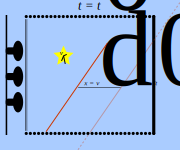
\includegraphics[width=0.48\textwidth]{images/Detector/CosmicPileup2.pdf}
        \label{fig:CosmicPileup2}
    } \\
    \subfloat[Cosmic-Ray Particle Interaction][Another cosmic-ray particle interaction at $t_\text{a}$]
    {
        \includegraphics[width=0.48\textwidth]{images/Detector/CosmicPileup3.pdf}
        \label{fig:CosmicPileup3}
    }
    \subfloat[Reconstructed Beam Event for $t_{0}$][Reconstructed beam event for $t_{0}$]
    {
        \includegraphics[width=0.48\textwidth]{images/Detector/CosmicPileup4.pdf}
        \label{fig:CosmicPileup4}
    }
    \caption[Cosmic Background Pileup]{Above series of figures shows the cosmic background pileup process. \subref{fig:CosmicPileup1} In the beginning at $t=t_\text{c}$, a cosmic particle crosses the active volume of the \gls{tpc} permeating through the cathode. \subref{fig:CosmicPileup2} Then, the ionisation track drifts towards the anode, when suddenly a beam related neutrino interaction occurs at $t=t_0$. \subref{fig:CosmicPileup3} Thereafter, both event signatures drift on as another cosmic-ray particle crosses the chamber, but this time permeating through the anode. \subref{fig:CosmicPileup4} When the event is reconstructed to match the beam event at $t=t_0$, both cosmic-ray related events are mis-projected on the drift axis, seemingly creating fake \glspl{Vertex}. In all four figures, the opaque lines show the position of the charge track at time $t$ and the faint, transparent lines show the true position of the track's origin. The yellow star symbolises the light \gls{Flash} produced by the interactions.}
    \label{fig:CosmicPileup}
\end{figure}
In the domain of \glspl{lartpc}, an event is always reconstructed to the time $t_0$ of a respective beam interaction, wherefore cosmic-ray related background events are usually mis-projected on the drift axis. The pileup of apparent \glspl{Vertex} of cosmic events piercing through anode or cathode constitute one of the major backgrounds of surface detectors with high cosmic-ray flux, like MicroBooNE. Deep underground experiments are naturally not subject to this particular background, as the cosmic-ray flux at their location is heavily reduced. At the time of MicroBooNE's conception, said background was not identified as a problem, although a cosmic-ray muon rate of \SI{5.5}{\kilo\hertz} in the \gls{tpc} leads to an expected \num{13} potential background events in a single readout window of \SI{2.25}{\milli\second} \cite{MicroBooNEMuonRate}. Even more disconcerting, the MicroBooNE proposals \cite{MicroBooNEProposal1, MicroBooNEProposal2} only identified advantages of the \gls{lartpc} technology vis-a-vis a Cherenkov detector, \eg the aforementioned electron-photon discrimination (see section \ref{sec:EnergyDissipationNeutral}). The importance of reducing the cosmic pileup background will be discussed in a small cosmic-ray photon study I performed in chapter \ref{sec:CosmicRayGammaBackground}.

There are, however, two methods to mitigate the above described background. One of these is utilising the light readout system to identify the various scintillation \glspl{Flash} and their origin. Once the \gls{Flash} is matched to its respective charge signal, the latter can be projected correctly to its location of incidence. This so-called \gls{Flash}-matching becomes really challenging with increasing background event numbers, as the misidentification probability of fake \glspl{Vertex} rises \cite{MicroBooNEFlashMatching}. Moreover, there are \glspl{Flash} that are not related to any charge signal, since light readout systems are usually sensitive to more than just the active volume. Depending on the accuracy and method of \gls{Flash}-matching, this background rejection method may lead to a noticeable loss in detector sensitivity, \ie many beam related events get discarded as well. A second method employs tracking detectors outside of the \gls{tpc}. Said external detector needs to be able to tag a cosmic event in space and time in order to correlate it with the \gls{tpc} signals. Such a \gls{crt} system was proposed and built by our group at \gls{lhep} \cite{CRTGeneral}. Cosmic-ray tagging and \gls{Flash}-matching are then combined, in order to increase the matching probability and decrease the beam event rejection. MicroBooNE's \gls{crt} system will be described in detail, later on in this thesis in section \ref{sec:CRT}.

\section{Space Charge Effect} \label{sec:SpaceCharge}
In section \ref{sec:ChargeDrift}, I introduced the rather low \ch{Ar2^+} mobility, $\mu_{0,\text{i}} = \SI{1.5e-3}{\centi\metre\squared\per\volt\per\second}$ which, consequently, leads to long dwell times of said ions in a \gls{tpc}. For a full drift in a \gls{tpc} with several metre drift distance, said dwell times are of the order of \SI{10}{\minute}. Hence, cosmic rays, constantly producing electron-ion pairs in the active volume, lead to an accumulation of continuous clouds of positively charged argon dimers. Such ion clouds are called \textbf{space charge} and were first discovered in the early 1900s in gas diodes \cite{SpaceChargeDiscovery1,SpaceChargeDiscovery2}. If the production of space charge is high enough, it will ultimately lead to distortions in the drift electric field, $\vec{E}$. In noble liquid detectors, said distortions were first observed in liquid krypton calorimeter prototypes for the NA48 experiment at CERN \cite{SpaceChargeDiscovery3}. In the context of these NA48 related measurements, S. Palestini \etal produced a model describing the influence of space charge on the drift field \cite{LArSpaceCharge1}, which I will later discuss here in more detail. In \gls{lar}, the space charge effect was first observed in a thin-gap ionisation chamber \cite{LArSpaceChargeDiscovery}. Both these noble liquid experiments featured short drift distances of \SI{1}{\centi\metre} and \SI{100}{\micro\metre}, respectively. Hence, the respective detectors had to be subject to intense radiation, in order for the space charge effect to become noticeable. For \glspl{lartpc} with drift distances of several metres, the effect becomes perceivable at much lower activity. For surface detectors with small overburden, even cosmic radiation is enough to induce the effect, as MicroBooNE has shown \cite{LArLaserMicroBooNE1,LArLaserMicroBooNE2,LArSpaceChargeMicroBooNE}. The MicroBooNE collaboration came up with their own, simplified model to describe the influence of space charge on the drift field. Unfortunately, the collaboration failed to explain the thinking behind said model and contrast it to the work of Palestini \etal. I would like to resolve this deficiency in this section.

First let us quantify said space charge effect on the electric field with the Palestini model. Palestini \etal \cite{LArSpaceCharge1,LArSpaceCharge2} realised that the space charge density has to follow the continuity equation,
\begin{equation}
    \frac{\partial \rho_\text{i}}{\partial t} + \vec{\nabla}\cdot \vec{j}_\text{i} = J.
\end{equation}
Here, $\rho_\text{i}$ stands for the ion density, $\vec{j}_\text{i}$ for the ion flux, and $J$ for the source, \ie the ion generation per unit volume per unit time. In our case, $J$ is deemed to be constant in time and position, as it is determined by the constant flux of cosmic-rays traversing the active volume. The term $\partial \rho_\text{i}/\partial t$ represents the time dependent variation of the charge density and finally $\vec{\nabla}\cdot \vec{j}_\text{i}$ describes the flow of ions, \ie how the charge carriers are transported out of the active volume by their drift. Since the space charge is considered in a velocity field, we can define the flux as $\vec{j}_\text{i} = \rho_\text{i}\vec{v}_\text{i}$. Furthermore, we can simplify above equation, if we think of the \gls{tpc} as an infinite parallel plate capacitor. In that case, $\rho_\text{i}$ and $\vec{v}_\text{i}$ only exhibit a drift coordinate, $x$, dependency. Hence, we reduce the problem to one dimension and replace $\vec{v}_\text{i}$ with $v_x$. Moreover, due to the constant generation of ions, $J$, the space charge concentration in the detector is expected to become stable after a certain time of operation. This stationary solution of the continuity equation, \ie $\partial \rho_\text{i} / \partial t = 0$, is of particular interest, for it describes the equilibrium state all \glspl{tpc} are operated in. Thus, above equation takes the form
\begin{equation} \label{eq:ContinuityEquation}
    \frac{\partial(\rho_\text{i} v_x)}{\partial x} = J.
\end{equation} 
Now we can use the mobility relation for the drift velocity, $v_x = \mu_{0,\text{i}} E_x$ from equation \ref{eq:DriftVelocity}, and integrate
\begin{align} \label{eq:StationaryContinuityEq}
    \int d(\rho_\text{i} E_x)\ \mu_{0,\text{i}} &= \int dx\ J, \nonumber \\[5pt]
    \Longrightarrow \ \mu_{0,\text{i}} \rho_\text{i} E_x &= J x + A.
\end{align}
Here $E_x$ stands for the drift coordinate component of the electric field, and $A$ for the integration constant. At the anode, \ie $x=0$, we expect $\rho_\text{i} = 0$, and thus get $A = 0$ as well. In order to obtain the connection between $\rho_\text{i}$ and $E_x$, it is useful to employ the \gls{1d} form of the first Maxwell equation, 
\begin{equation} \label{eq:MaxwellEquation1D}
    \frac{\partial E_x}{\partial x} = \frac{\rho_\text{i}}{\epsilon_0\epsilon_\text{r}},
\end{equation}
with $\epsilon_0\epsilon_\text{r}$ again representing the dielectric constant of \gls{lar}. By replacing $\rho_\text{i}$ of equation \ref{eq:StationaryContinuityEq}, we arrive at our final, solvable differential equation for $E_x$ with
\begin{equation}
    \epsilon_0\epsilon_\text{r}\mu_{0,\text{i}}E_x\frac{\partial E_x}{\partial x} = J x.
\end{equation}
Solving above equation with the proper boundary conditions for the integration constants results in \cite{LArSpaceCharge1}
\begin{equation} \label{eq:PalestiniField}
    E_x(x) = E_0 \sqrt{\left(\frac{E_\text{a}}{E_0}\right)^2 + \alpha^2 \left(\frac{x}{L}\right)^2}, \qquad \text{with} \quad \alpha = \frac{L}{E_0}\sqrt{\frac{J}{\epsilon_0\epsilon_\text{r}\mu_{0,\text{i}}}}.
\end{equation}
In above equation, $E_0$ denotes the electric field strength without space charge, $E_\text{a}$ the field strength at the anode (with space charge), and $L$ the full drift distance of the \gls{tpc}. The electric field at the anode, $E_\text{a}$, can be calculated using the boundary condition given by the applied cathode voltage $V_0$
\begin{equation} \label{eq:AnodeBoundaryCondition}
    V_0 = -\int_{0}^{L} dx \ E_x(x).
\end{equation}
Since above integral leaves us with no analytical solution for $E_\text{a}$, there is an numerical approximation given by \cite{LArSpaceCharge2}
\begin{equation}
    E_\text{a} = 
    \begin{cases}
        E_0\left( 1-\alpha^2/6-\alpha^4/180 \right) & \text{for} \ \alpha < 1.57 \\
        E_0\left( 1-\alpha^2/6-\alpha^4/180-\alpha^6/8500 \right) & \text{for} \ \alpha < 1.89
    \end{cases},
\end{equation}
For $\alpha > 2$, the Palestini model reaches its limit as $E_\text{a} < 0$, \ie the charge density gets high enough, that the electric field at the anode would reverse. In case of such an extreme space charge concentration in the active volume, the \gls{tpc} would simply cease functioning. With $E_x(x)$ established, it is then quite simple to derive the charge density distribution, $\rho_\text{i}(x)$ by again making use of the \gls{1d} Maxwell equation \ref{eq:MaxwellEquation1D} and get
\begin{align}
    \rho_\text{i}(x) &= \epsilon_0\epsilon_\text{r}\,\frac{\partial E_x(x)}{\partial x} \nonumber \\
    &= \alpha^2 \epsilon_0\epsilon_\text{r} \, \frac{E_0^2}{E_x(x)} \frac{x}{L^2}.
\end{align}

MicroBooNE's approach assumes the space charge density to be linear in the drift coordinate, $x$, \ie $\rho_\text{i}(x) = a x$ \cite{LArSpaceChargeMicroBooNE}. Even before MicroBooNE, I myself used the same linear approximation in my master's thesis \cite{LArTPCMasterChristoph}. It is the logical first order solution, if one considers a constant drift velocity and a constant ionisation rate in the chamber. However, myself and the MicroBooNE collaboration failed to connect this assumption to the continuity equation, as we did not research the topic properly. The key difference between the MicroBooNE approximation and the Palestini model is the assumption that $v_x$ is constant. All other assumptions stay the same. Pertaining the continuity equation in \ref{eq:ContinuityEquation}, MicroBooNE's first order approximation takes the form
\begin{align}
    v_x\,\frac{\partial\rho_\text{i}}{\partial x} &= J, \nonumber \\
    \Longrightarrow \ \rho_\text{i}(x) &= \frac{J}{v_x}x
\end{align}
The integration constant of above relation equates to zero, as $\rho_\text{i}(0) = 0$. From here MicroBooNE uses \gls{3d} numerical integration in order to get to the solution for the electric field. Since I would like to compare the MicroBooNE approximation to the Palestini model, I proceed to calculate $E_x$ using equation \ref{eq:MaxwellEquation1D} and get
\begin{align}
    E_x(x) &= \int dx \ \frac{\rho_\text{i}(x)}{\epsilon_0\epsilon_\text{r}} \nonumber \\
           &= E_\text{a} + \frac{J}{2v_x\epsilon_0\epsilon_\text{r}}x^2.
\end{align}
Here I also used the boundary condition at $x=0$ to determine the integration constant as $E_\text{a}$. This time, however, $E_\text{a}$ can be obtained analytically by solving equation \ref{eq:AnodeBoundaryCondition} like
\begin{align}
    V_0 &= -\int_{0}^{L} dx \ E_x(x), \nonumber \\
        &= -E_\text{a} L - \frac{J}{6v_x\epsilon_0\epsilon_\text{r}} L^3, \nonumber \\[5pt]
    \Longrightarrow \ E_\text{a} &= E_0 - \frac{J}{6v_x\epsilon_0\epsilon_\text{r}} L^2.
\end{align}
In the last step of above derivation, I used the relation $E_0 = -V_0/L$. With both models established, we can now compare their solutions for $\rho_\text{i}(x)$ and $E_x(x)$, shown in figure \ref{fig:SpaceChargeModels}, using MicroBooNE's detector specifications. MicroBooNE exhibits a space charge source of $J = \SI{1.6e-10}{\coulomb\per\metre\cubed\per\second}$ \cite{LArSpaceChargeMicroBooNE}, a cathode voltage of $V_0 = \SI{-70}{\kilo\volt}$, a full drift length of $L = \SI{256}{\centi\metre}$, and thus an electric field strength without space charge of $E_0 = \SI{273.4}{\volt\per\centi\metre}$.
\begin{figure}[htbp]
    \centering
    \subfloat[Space Charge Density][Space charge density]
    {
        \includegraphics[width=1.0\textwidth]{images/Detector/SpaceChargeDensity.pdf}
        \label{fig:SpaceChargeDensity}
    } \\
    \subfloat[Electric Field Distortion due to Space Charge][Electric field distortion due to space charge]
    {
        \includegraphics[width=1.0\textwidth]{images/Detector/SpaceChargeField.pdf}
        \label{fig:SpaceChargeField}
    }
    \caption[Space Charge Models]{These graphs illustrate the Palestini model and the MicroBooNE approximation of the space charge density $\rho_\text{i}(x)$ \subref{fig:SpaceChargeDensity} and the resulting electric field strength on the drift axis $E_x(x)$ \subref{fig:SpaceChargeField}. In order to emphasise the field distortions introduced by space charge, the constant design field strength $E_0$ is shown as a red line in \subref{fig:SpaceChargeField}. All models are drawn, using MicroBooNE detector specifications.}
    \label{fig:SpaceChargeModels}
\end{figure}
% TODO add correlation factor?
As can be seen in figure \ref{fig:SpaceChargeDensity}, MicroBooNE's approximation of the Palestini model and the Palestini model itself are quite close for $x<\SI{150}{\centi\metre}$, concerning the space charge density. Thereafter, towards the cathode, they start to diverge with a maximum $\rho_\text{i}(x)$ difference of $\sim\SI{20}{\percent}$. However, this difference is much smaller when considering $E_x(x)$ of both models, as shown in figure \ref{fig:SpaceChargeField}. As an approximation for $E_x(x)$, MicroBooNE's approach is certainly usable, although the Palestini model is still preferable in my opinion, since it is more accurate and does not complicate calculations significantly, \ie why simplify a model that is already simple to solve. Comparing the two field strength curves $E_x(x)$ to the constant $E_0$ in \ref{fig:SpaceChargeField}, it becomes obvious how space charge distorts the field. It lowers $E_x(x)$ at the anode, but leads to an increase at the cathode. As stated before, both models do not take into account the field components in the $y$ and $z$ coordinates. Therefore, both models are only valid in the very centre of the detector's $y$-$z$ coordinates, for the field cage elements introduce non-zero values for $E_y$ and $E_z$. Thus, the MicroBooNE collaboration's decision to use full \gls{3d} integration of the charge density in order to determine the electric field is certainly increasing the accuracy of the model. Furthermore, non-zero values for $E_y$ and $E_z$ also means non-zero values for $v_y$ and $v_z$ which in turn again influences the charge density distribution. Still, if $E_{y,z} \ll E_x$, the effect on the space charge density might be minimal. One open point that remains unaddressed, is the change in the flux $\vec{j}$, or $\vec{v_i}$ respectively, due to fluid currents in \gls{lar}. Said currents are induced by convection and the recirculation of \gls{lar} and are of the same order of magnitude as the drift velocity. These partially random currents are very difficult to measure or simulate. Hence, there might never be a complete model to describe the space charge effect in a \gls{lartpc}.

It is impossible to compensate for the space charge effect in a \gls{tpc} with adaptations of the field cage design, because of the randomness of the \gls{lar} flow. The only way to mitigate the severity of the effect is to choose a small drift distance. Since this would also increase the numbers of readout channels for the instrumentation of the same volume, smaller drifts are often not preferable. However, the drift field distortion, caused by space charge, can be measured using the ionisation track of an \gls{uv} laser beam as introduced in section \ref{sec:MultiPhotonIonisation}. The positional distortion of the recorded events can be directly measured as the displacement of the laser track within the active volume. For this to work, the true position and direction of the laser beam needs to be determined to high accuracy. Said true track then has to be compared, in a discrete manner, with the apparent position of the reconstructed track after completion of the \gls{tpc}'s readout process. In such an arrangement, the \gls{3d} displacement vector is then defined as
\begin{equation} \label{eq:DisplacementDefinition}
    \vec{d}_i \coloneqq \vec{t}_i - \vec{r}_i,
\end{equation}
where $i$ denotes the index of a discrete reconstructed track point, $\vec{r}_i$, and its associated position on the true laser track, $\vec{t}_i$. There is, however, a problem: we only know two parameters of the true laser track, the entry point, $\vec{L}_\text{entry}$, and the exit point, $\vec{L}_\text{exit}$, from the active volume. This leads to ambiguities for the true position, $\vec{t}_i$, as in principle every position along the true track between $\vec{L}_\text{entry}$ and $\vec{L}_\text{exit}$ could be chosen. Yet, $\vec{t}_i$ can be approximated, assuming the displacement, $\vec{d}_i$, to be minimal, \ie $\vec{d}_i \perp (\vec{L}_\text{exit} - \vec{L}_\text{entry})$. Therefore, we can rewrite equation \ref{eq:DisplacementDefinition} as
\begin{equation} \label{eq:DisplacementEquation}
    \vec{d}_i = \vec{L}_\text{entry} + \alpha_i\left(\vec{L}_\text{exit} - \vec{L}_\text{entry}\right) - \vec{r}_i.
\end{equation}
Since, in our example, the displacement is perpendicular to the true laser track, we can use $\vec{d}_i \cdot (\vec{L}_\text{exit} - \vec{L}_\text{entry}) = 0$ to solve for the scaling factor $\alpha_i$, resulting in
\begin{equation}
    \alpha_i = \frac{\left(\vec{r}_i - \vec{L}_\text{entry}\right) \cdot \left(\vec{L}_\text{exit} - \vec{L}_\text{entry}\right)}{\left\vert\vec{L}_\text{exit} - \vec{L}_\text{entry}\right\vert^2}.
\end{equation}
Other approximation methods, \eg $\vec{d}_i \perp \vec{r}_i$, would lead to other constraints and hence different solutions for $\alpha_i$. A \gls{2d} representation of the above-described procedure to determine the displacement is shown in figure \ref{fig:LaserCallibrationMethod}.
\begin{figure}[htbp]
    \centering
    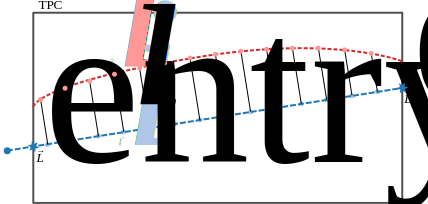
\includegraphics[width=\textwidth]{images/Detector/LaserCallibrationMethod.pdf}
    \caption[Displacement Measurement Method]{Shown here, is a schematic view of a displacement measurement method employing a laser system in \gls{lar}. The true laser path is shown in blue, and the due to space charge distorted \gls{quasifreeelectron} track in red. Above figure was originally drawn by M. L\"uthi for his PhD Thesis \cite{LArLaserPhDMatthias} and slightly adapted.}
    \label{fig:LaserCallibrationMethod}
\end{figure}
Whichever method is chosen, the ambiguities on the beam axis can not be avoided, but there are no ambiguities in the plane perpendicular to the true track. Thus, a second laser beam, ideally perpendicular to the first one, can mitigate or even resolve these ambiguities. Said mitigation is done iteratively by correcting the track of the first laser in small steps with the displacement measured by the second one, and vice versa. Moreover, movable mirrors, as used in MicroBooNE, are able to provide a multitude of laser tracks with different angles which therefore cover a large part of the active volume.

With these vast amounts of recorded laser tracks, one receives a large set of irregularly spaced reconstructed points, $\vec{r}_{n,m}$, each with a displacement vector, $\vec{d}_{n,m}$. Here, $n$ is the track number and $m$ the track point index introduced above. This irregularity is unfavourable for our purpose, as we aim to not only reconstruct the displacement, but also the electric field. Hence, an equally spaced \gls{3d} grid, called displacement map, needs to be created by applying an elaborate interpolation algorithm. Said algorithm first creates a mesh of all irregular points employing Delaunay refinement. Then, the regular grid points are interpolated using barycentric coordinates within the mesh. I will skip the exact formalism of this procedure in this work, for it is already documented in great detail \cite{LArLaserMicroBooNE2,LArLaserPhDMatthias,LArLaserPhDYifan}.

In this regular grid, called displacement map, we now end up with three indices for all three dimensions, $i$ for the $x$, $j$ for the $y$, and $k$ for the $z$-component of the map. The displacement vector is therefore denoted as $\vec{d}_{i,j,k}$. The spacing of the grid points is, as mentioned before, regular with a size of $\Delta x$. On the drift axis ($x$-axis) the grid spacing is connected to the drift time,$\Delta t$ by $\Delta x = v_\text{d}\Delta t$, with $v_\text{d}$ denoting the constant drift velocity of the \gls{quasifreeelectron} disregarding field distortions. Now, in order to reconstruct the drift electric field, we first need to derive the drift velocity from the displacement map. This is done in reverse to the drift process, starting at the anode and ending at the cathode, using the displacement difference of two adjacent points on the drift axis
\begin{equation} \label{eq:DisplacementDifference}
    \vec{R}_{i,j,k} \coloneqq \vec{d}_{i+1,j,k} - \vec{d}_{i,j,k}.
\end{equation}
As a matter of fact, $\vec{R}_{i,j,k}$ describes the movement of the drifted charge carriers within the time window $\Delta t$. From this it is straight forward to evaluate the drift velocity for each grid point as
\begin{align} \label{eq:VelocityDistortion}
    \vec{v}_{i,j,k} &= -\frac{1}{\Delta t} \vec{R}_{i,j,k}, \nonumber \\[5pt]
    \Longrightarrow \ \vec{v}_{i,j,k} &= -\frac{v_\text{d}}{\Delta x} \vec{R}_{i,j,k}.
\end{align}
As can be seen, the drift velocity points in the opposite direction of the displacement difference. Furthermore, above method assumes a constant displacement and hence a constant drift velocity within two grid points. Said assumption is valid, if $\Delta x$ is smaller than the expected magnitude of $\vec{d}$. The above described calculation are visualised as a simplified \gls{2d} depiction in figure \ref{fig:LaserVelocityCallibration}.
\begin{figure}[htbp]
    \centering
    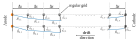
\includegraphics[width=\textwidth]{images/Detector/LaserVelocityCallibration.pdf}
    \caption[Drift Velocity Distortion Measurement Method]{Depicted here is the drift velocity distortion measuring method as a \gls{2d} simplification. It uses the displacement differences $\vec{R}_{i,j}$ in a regular grid and applies them to equation \ref{eq:VelocityDistortion}. Again, the original is sourced from M. L\"uthi's Thesis \cite{LArLaserPhDMatthias} and slightly altered.}
    \label{fig:LaserVelocityCallibration}
\end{figure}
From here, it is quite simple to calculate the electric field map, $\vec{E}_{i,j,k}$ by using $\vec{v}_{i,j,k}$ and solving the mobility relation of equation \ref{eq:DriftVelocity}. For small field deviations we can even use a constant mobility, in order to simplify calculations. With the displacement, and field maps established, we can now correct particle track positions as well as drift field related effects like recombination. In a surface detector exhibiting the dimensions of MicroBooNE, displacements reach about \SI{15}{\centi\metre} and electric field distortions are found in the vicinity \SI{30}{\volt\per\centi\metre} \cite{LArLaserMicroBooNE2}.

During my time with MicroBooNE, the electric field and displacement calibration became my main task, especially the analysis side. I wrote the software which calculates the displacement and interpolates the grid points. Still, I decided to only include this small summary of this topic, as my colleagues brought the analysis methods to their final form and documented them well in their excellent theses \cite{LArLaserPhDMatthias,LArLaserPhDYifan}.
\end{fmffile} % Close the feynman diagram file


    % detector setup
    %TODO Check if 470m or 473m distance between detector and target (or even decay tunnel)
\chapter{Experimental Setup} %\label{sec:ExperimentalSetup}
MicroBooNE marks the first experiment of the \gls{lartpc} based \gls{sbn} at \gls{fnal}. The detector is located in the \gls{bnb}. Since neutrinos lack electromagnetic charge, they can not be accelerated directly with any technology known to humanity. Thus a complex accelerator system is employed to produce high energy protons, which are then collided onto a target. The products of said collision then decay \ia into neutrinos. A site map of the \gls{bnb} beam line and MicroBooNE is shown in figure \ref{fig:MicroBooNELocation}. As the above description is rather rudimentary, I would like to give a more detailed insight into the \gls{bnb} in the following paragraphs. Thereafter, I will discuss the MicroBooNE detector and its various subsystems.
\begin{figure}[htbp]
    \centering
    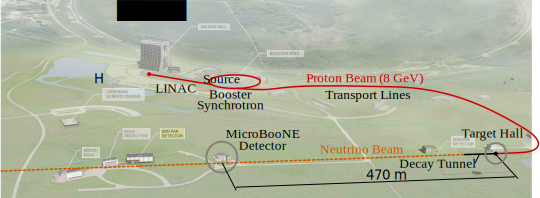
\includegraphics[width=1.0\textwidth]{images/MicroBooNE/MicroBooNELocation.pdf}
    \caption[Site map of the MicroBooNE Detector and the Booster Neutrino Beam Line]{Shown above is a site map of the MicroBooNE detector and the \gls{bnb} line. The beam line starts close to Wilson Hall at the \ce{H-} source (red dot). Then these ions and later protons are accelerated by the \gls{linac} and the Booster to \SI{8}{\giga\electronvolt} (red line). Thereafter transport lines (also red) guide the proton beam to the target (black dot). There the protons collide and produce, among other particles, pions and kaons. These then further decay into neutrinos and charged leptons in the decay tunnel (black line). The neutrinos traverse the rock (dashed orange line) and cross the detector after \SI{470}{\metre}. The original picture was sourced from \cite{MicroBooNEDetector} and modified.}
    \label{fig:MicroBooNELocation}
\end{figure}

\section{Booster Neutrino Beam} \label{sec:BNB}
Like many other high energy particle beams, the \gls{bnb}'s origin is an inconspicuous pressurised gas cylinder containing hydrogen gas, \ce{H2}. This hydrogen is then fed into a \textbf{dimpled magnetron} \cite{BNBProtonSource1,BNBProtonSource2}, where a dense plasma is produced. The electrons in the plasma are confined to spiral around the magnetron's cavity, while the protons are attracted by the cathode made of neodymium \cite{BNBProtonSource2}. A constantly reapplied caesium coating notably lowers the \gls{WorkFunction} of the cathode surface, such that the protons are able to acquire two electrons when impacting the surface. Thus, negatively charged hydrogen atoms, \ce{H-}, are formed which are then immediately repelled by the cathode \cite{BNBProtonSource1}. Through an aperture in the anode, the \ce{H-} ions are able to escape from the magnetron. In order to increase the efficiency of the \ce{H-} source, a spherical dimple is carved into the cathode opposite of the aperture, \ie said dimple has a focusing effect on the ions and facilitates their escape through the gap. In addition, a pulsed extractor cone, placed out side of the magnetron at the aperture, further increases the extraction yield and accelerates the \ce{H-} ions to a kinetic energy of \SI{35}{\kilo\electronvolt}. Said \ce{H-} extraction is pulsed to \SI{15}{\hertz} with a pulse width of \SI{230}{\micro\second} \cite{BNBProtonSource2,BNBProtonSource3}. From here, the low energy beam is guided into a four-rod \gls{rfq} injector, which is still considered part of the \ce{H-} source system. In principle the \gls{rfq} is a linear accelerator, within which an electromagnetic standing wave of \SI{201.25}{\mega\hertz} accelerates the \ce{H-} ions to a kinetic energy of \SI{750}{\kilo\electronvolt} \cite{BNBProtonSource4}. The beam current generated by above-described \ce{H-} source assembly is \SI{60}{\milli\ampere} \cite{BNBProtonSource3}. The \ce{H-} source is shown as a red dot, at the start of the proton beam line in figure \ref{fig:MicroBooNELocation}.

From the \ce{H-} source, the beam is transferred to the \gls{fnal} \gls{linac}, a series of linear particle accelerators. The \gls{linac} is comprised of five Alvarez drift tube cavities operated at \SI{201.24}{\mega\hertz} \cite{BNBLinac1} followed by seven high-frequency (\SI{805}{\mega\hertz}) side-coupled cavity structures \cite{BNBLinac2}. As the frequencies indicate, both technologies are powered by high-intensity radio waves, which induces an alternating electric field in these \gls{rf} cavities synchronised to the particle's motion. This way, the drift tube section accelerates the \ce{H-} beam to a kinetic energy of \SI{116.5}{\mega\electronvolt} while the side-coupled cavities increases their kinetic energy further to \SI{400}{\mega\electronvolt} \cite{BNBLinac3}. Naturally, the \gls{linac} is also pulsed to \SI{15}{\hertz} and synced to the \ce{H-} source cycles. These pulses are not to be confused with the beam bunches, \ie the fine structure of the pulses introduced by the cavity's \gls{rf}, \SI{805}{\mega\hertz} in the case of the \gls{linac}. The schematics of above-described \gls{linac} can be inferred from figure \ref{fig:Linac} and its location from figure \ref{fig:MicroBooNELocation}.
\begin{figure}[htbp]
    \centering
    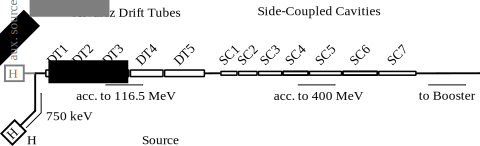
\includegraphics[width=1.0\textwidth]{images/MicroBooNE/LinacSchematics.pdf}
    \caption[Schematics View of the Linac]{This graph shows a schematics view of \gls{fnal} \gls{linac}. The \ce{H-} ions leave the source with an kinetic energy of \SI{750}{\kilo\electronvolt}. These ions are then first accelerated to \SI{116.5}{\mega\electronvolt} by Alvarez drift tubes (DT1 through DT5), and then further accelerated to \SI{400}{\mega\electronvolt} by side-coupled cavities (SC1 through SC7). This schematic view is inspired by \cite{BNBLinac3}.}
    \label{fig:Linac}
\end{figure}

Before the particles are accelerated further, they pass through a thin foil made of carbon. Said foil causes the stripping of all electrons from the \ce{H-} ions, thus yielding a pure proton beam \cite{BNBBooster1}. Thereafter, the protons are injected into the Booster synchrotron ring with a circumference of \SI{474.2}{\metre} \cite{BNBBooster2}. Acceleration in the Boster ring occurs in three steps \cite{BNBBooster1}:
\begin{enumerate}
    \item Injection from the \gls{linac}, and bunching within \SI{2}{\milli\second}.
    \item Acceleration, lasting about \SI{29}{\milli\second}.
    \item Eventual phase locking with the next accelerator stage and extraction in \SI{2.5}{\milli\second}.
\end{enumerate}
Above cycle is repeated every \SI{1/15}{\second}, in sync with the \gls{linac} injection of \SI{15}{\hertz}. In the injection phase, the proton's energy spread of about \SI{0.3}{\percent}, introduced by the \gls{linac}, is first reduced and with it, the \gls{linac}'s \SI{805}{\mega\hertz} bunch structure disappears as well. The Booster ring features \num{17} ferrite-tuned resonator \gls{rf} cavities as accelerators located in one half of the ring. In contrast to the \gls{linac} and the \gls{rfq}, these Booster cavities feature variable frequencies. Right after injection, the Booster's \gls{rf} cavities operate at \SI{37.86}{\mega\hertz} and the \SI{400}{\mega\electronvolt} proton beam requires \SI{2.2}{\micro\second} to complete a full revolution of the ring. Dipole magnets along the sychrotron's circumference keep the beam in its orbit. In order to increase the kinetic energy of the protons, the frequency in the \gls{rf} cavities needs to be raised slowly and with it, the magnetic field of the dipoles in order to stabilise the beam on its trajectory. At the end of the \SI{29}{\milli\second} acceleration cycle, the cavity frequency reaches \SI{52.81}{\mega\hertz}. In this process the proton kinetic energy reaches \SI{8}{\giga\electronvolt} and the full ring revolution time is reduced to \SI{1.6}{\micro\second}. The latter also gives us the pulse width of the beam, while it contains \num{84} bunches given by the frequency of the cavities. Since the \gls{bnb} does not use higher energy protons than the ones provided by the Booster, the phase locking before extraction is not required. The extraction of the beam from the synchrotron ring is accomplished by fast switching magnets (\SI{40}{\nano\second} rise time), called \textbf{kickers}. During the whole acceleration process, a multitude of beam optics magnets is used to stabilise the beam on its trajectory. All the aforementioned Booster properties are sourced from \cite{BNBBooster1,BNBBooster2}. The location of the Booster synchrotron can be extracted from figure \ref{fig:MicroBooNELocation}.

From the Booster, the \SI{8}{\giga\electronvolt} proton beam pulses are guided with a frequency of \SI{15}{\hertz} to the various experiments or to additional accelerators. In the \gls{bnb}'s case, at most every third Booster pulse is routed through transport lines and various beam optics elements to the target hall, as indicated in figure \ref{fig:MicroBooNELocation}. This leads to a \gls{bnb} beam pulse frequency of $f_\text{BNB} \leq \SI{5}{\hertz}$. At the target hall, the proton beam is extracted from beam vacuum pipes into air and after \SI{1.5}{\metre} collided onto a beryllium target \cite{BNBBeamFlux}. The full target assembly is shown in figure \ref{fig:BNBTarget}.
\begin{figure}[htbp]
    \centering
    \includegraphics[width=1.0\textwidth]{images/MicroBooNE/BNBTarget.pdf}
    \caption[Technical Drawing of the BNB Target]{This figure depicts a technical drawing of the \gls{bnb} beryllium target, sourced from \cite{BNBBeamFlux}. In the side view, the proton beam hits the target from the left hand side.}
    \label{fig:BNBTarget}
\end{figure}
This main target structure is composed of seven identical so-called \textbf{target slugs} placed in a row along the proton beam axis. These slugs are beryllium cylinders with a diameter of \SI{9.525}{\milli\metre} featuring three regularly spaced fins. Said fins hold the target in the centre of a surrounding tube and provide air-cooling. Beryllium is chosen because of its relatively low atomic number, $Z$, and its low density, $\rho$, which lead to a low \textbf{linear stopping power} for charged particles according to the \textbf{Bethe equation} \ref{eq:BetheBloch}. This is advantageous as the aim is to spend most of the energy as possible for neutrino production rather than ionisation. Furthermore, beryllium features low residual radioactivity after being exposed to a proton beam and it allows for air cooling, reducing the complexity of the target system \cite{BNBBeamFlux}. Before the collision, the proton beam gets focused on the cylindrical part of the upstream target slug. This leads to maximum collision yield of \num{5e12} \gls{pot} per beam pulse \cite{BNBBeamFlux}. 

The above-described target assembly is embedded into a so-called \textbf{horn electromagnet}. Said horn is, simply put, a hollow cylinder with electrically conducting surfaces. At the upstream end of the cylinder, the inner and outer surfaces are electrically insulated. Now, if power is applied across said insulation, a current will flow from the inner conductor layer to the outer in neutrino mode or vice-versa in anti-neutrino. This current then induces a toroidal magnetic field, $\vec{B}$, which falls with $1/R$, where $R$ is the radial distance from the cylinder axis. A cutaway view of the above described horn electromagnet is shown in figure \ref{fig:BNBNeutrinoProduction}. The \gls{bnb} horn is composed of an aluminium alloy. The horn's current is pulsed to \SI{5}{\hertz} with a pulse length amounting to \SI{143}{\micro\second}. Naturally, the current pulse is synchronised with the arrival of the Booster proton beam. At its peak the horn current reaches \SI{174(1)}{\kilo\ampere}, resulting in a maximum magnetic field strength $B_\text{max} = \SI{1.5}{\tesla}$ \cite{BNBBeamFlux}. The \gls{bnb} horn is situated in front of a \SI{45}{\metre} long air-filled decay tunnel, also shown in figure \ref{fig:BNBNeutrinoProduction}. From the upstream face of the target to the beam stop at the end of the decay tunnel the distance amounts to \SI{50}{\metre}.
\begin{figure}[htbp]
    \centering
    \includegraphics[width=1.0\textwidth]{images/MicroBooNE/BNBNeutrinoProduction.pdf}
    \caption[Neutrino Production Process at the BNB Target Hall]{This figure shows a schematic view of the neutrino production facility located at the target hall (not to scale), sourced from \cite{LArLaserPhDMatthias}. The drawing is cylindrically symmetrical along the proton beam axis. Here, the beryllium target (green) is inserted into a horn electromagnet (grey). The annular electrical insulation of the horn assembly is shown as brown spots. The aforementioned target and horn assembly is then placed in front of a \SI{45}{\metre} long decay tunnel. Now, if the proton beam (red) hits the target, a host of secondary particles are produced, here indicated by pions, $\pi^+$ (blue) and $\pi^-$ (purple). In the picture, the horn's magnetic field, $\vec{B}$, is polarised in neutrino mode. Hence positively charged particles are focused forward into the decay tunnel, while negatively charged particles are deflected to the side. In the decay tunnel, $\pi^+$ decays into a muon, $\mu$ (solid orange), and its neutrino, $\nu_\mu$ (dashed orange). Finally, most of the muons are stopped in the absorber where they decay.}
    \label{fig:BNBNeutrinoProduction}
\end{figure}

The primary \SI{8}{\giga\electronvolt} Booster protons produce a multitude of secondary particles interacting with the beryllium. These secondaries are predominantly composed of pions, $\pi^{\pm}$, charged kaons, $K^{\pm}$, neutral kaons, $K^0$, protons, $p$, and neutrons, $n$. Their respective production rate per proton-beryllium interaction is listed in table \ref{tab:BNBSecondaryComposition}.
\begin{table}[htbp]
    \centering
    \caption[BNB Secondary Particle Composition after Target Interaction]{This table lists the secondary particle composition after a single \SI{8}{\giga\electronvolt} proton-beryllium interaction in the \gls{bnb} target. Furthermore, the average secondary particle momentum, $\langle p \rangle$, and their average angle with respect to the primary proton beam axis, $\langle \theta \rangle$, are presented. This data is based on a \gls{mc} simulation performed for the MiniBooNE experiment \cite{BNBBeamFlux} and thus has to viewed with some healthy scepticism.}
    \begin{tabu} to 0.7\textwidth{X[-0.5c] X[c] X[-0.5c] X[-0.5c]} \toprule
        Secondary Particle & Multiplicity per \ce{$p$-Be} reaction & $\langle p \rangle$ $[\si{\giga\electronvolt\per\lightspeed}]$ & $\langle \theta \rangle$ $[\si{\milli\radian}]$ \\ \midrule
        $p$ & 1.5462 & 2.64 & 441 \\
        $n$ & 1.3434 & 1.59 & 586 \\
        $\pi^-$ & 0.9004 & 0.82 & 556 \\
        $\pi^+$ & 0.8825 & 1.11 & 412 \\
        $K^+$ & 0.0689 & 1.69 & 332 \\
        $K^0$ & 0.0241 & 1.34 & 414 \\
        $K^-$ & 0.0024 & 1.26 & 259\\ \bottomrule
    \end{tabu}
    \label{tab:BNBSecondaryComposition}
\end{table}
Of these secondary particles, only the \glspl{Meson} are of interest, since the baryonic secondaries, \ie $p$ and $n$, are not able to contribute to the neutrino production, due to their long lifetime. As the aforementioned table indicates, the substantial majority ($\sim \SI{95}{\percent}$) of secondary \glspl{Meson} are given by the charged pions. After their creation, most of the secondary pions scatter out of the beryllium target slugs with an average angle from the primary proton beam of $\langle \theta \rangle \approx \SI{24}{\degree}$ for $\pi^+$, and $\langle \theta \rangle \approx \SI{32}{\degree}$ for $\pi^-$, respectively. As they enter the horn electromagnet, they become subject to the strong magnetic field. Depending on the polarisation of the horn, one of the charges gets focused forward into the decay tunnel, while the opposite charge is deflected to the sides, as shown in figure \ref{fig:BNBNeutrinoProduction}. In neutrino mode, the horn's polarisation is such that $\pi^+$ are focused, while the $\pi^-$ are deflected. Since my thesis contains solely neutrino cross section measurements, I will omit the anti-neutrino mode from here on out.

Once in the decay tunnel, most of the positively charged secondary \glspl{Meson} decay in flight \ia into neutrinos. As an example for this process let us consider the decay modes of the two most prominent contributors \cite{PDG2018}
\begin{align}
    \ce{$\pi^{+}$ &->[\SI{99.99}{\percent}] $\mu^{+}$ +  $\nu_{\mu}$} \\
    \ce{$K^{+}$ &->[\SI{63.56}{\percent}] $\mu^{+}$ +  $\nu_{\mu}$}. \nonumber
\end{align}
Here the percentage denotes the fraction of said decay channel. The relatively high momentum of the secondaries, \ie average momentum $\langle p \rangle > \SI{1}{\giga\electronvolt}$, means that most of these secondary \glspl{Meson} are relativistic particles with a notable \textbf{Lorentz boost}. Thus, the decay products are focused forward when viewed in a reference frame at rest, as is the case here. In fact, it is these \textbf{Lorentz boosted} decay neutrinos which constitute the \gls{bnb}. Said neutrinos then traverses the rock due to the small interaction cross section. All the charged massive remnants of the above-described neutrino beam production process eventually loose their energy in the absorber and decay there at rest. The in flight decay process of a $\pi^+$ is also illustrated in figure \ref{fig:BNBNeutrinoProduction}.

So far we considered only the ideal neutrino production process, but in reality it is impossible to create a single flavour neutrino beam. Smart design choices, however, are able to reduce beam contaminants, \ie neutrinos of different flavour. The \SI{50}{\metre} decay distance, for instance, is optimised for allowing most $\pi^\pm$ and $K^\pm$ to decay within their typical lifetime of $\mathcal{O}(\SI{e-8}{\second})$), while preventing muon decays with a lifetime of $\mathcal{O}(\SI{e-6}{\second})$. The latter contaminate the beam with their two-neutrino decay signature \cite{PDG2018},
\begin{equation}
    \ce{$\mu^{+}$ ->[$\sim\SI{100}{\percent}$] $e^{+}$ + $\nu_{e}$ + $\bar{\nu}_{\mu}$}.
\end{equation}
The fact that most muons are stopped in the absorber, leads to a reduction of contaminants in the \gls{bnb}, as possible neutrinos originating from above decay at rest are not Lorentz boosted and thus radiate homogenously in all directions. Yet, the $\mu^+$ decays contribute the majority of $\nu_e$ contaminants in the \gls{bnb} \cite{BNBBeamFlux}. Another crucial design element, in regard of contaminants, is the horn electromagnet, which is responsible for deflecting the negatively charged secondaries. Then the horn is not able to deflect particles which stay within its inner conductor layer. Accordingly, the $\bar{\nu}_\mu$ beam impurity is introduced predominantly by the $\pi^-$ decay \cite{PDG2018},
\begin{equation}
    \ce{$\pi^{-}$ ->[\SI{99.99}{\percent}] $\mu^{-}$ +  $\bar{\nu}_{\mu}$}.
\end{equation}
According to simulations $\bar{\nu}_\mu$ represents the largest proportion of contaminants in the \gls{bnb} in neutrino mode with almost \SI{6}{\percent}, see table \ref{tab:BNBFluxComposition}. 
\begin{table}[htbp]
    \centering
    \caption[BNB Integrated Flux Composition]{Listed here is the expected \gls{bnb} integrated flux composition by neutrino flavour in neutrino mode at the MicroBooNE location. In neutrino mode, all neutrino flavours other than $\nu_\mu$ are considered beam contaminants or impurities. The beam fluxes presented here are the integrals of the graphs in figure \ref{fig:BNBFlux} and are sourced from \cite{BNBBeamUncertainty}.}
    \begin{tabu} to 0.6\textwidth{X[-0.4c] X[1.0c] X[-0.5c]} \toprule
        Neutrino Flavour & Integrated Flux $[\si{\per\centi\metre\squared\per\pot}]$ & Fraction $[\si{\percent}]$ \\ \midrule
        $\nu_\mu$ & \num{7.18(90)e-10} & \num{93.63} \\
        $\bar{\nu}_\mu$ & \num{4.45(60)e-11} & \num{5.81} \\
        $\nu_e$ & \num{3.91(46)e-12} & \num{0.51} \\
        $\bar{\nu}_e$ & \num{3.93(77)e-13} & \num{0.05} \\ \bottomrule
    \end{tabu}
    \label{tab:BNBFluxComposition}
\end{table}
Another impurity source are neutral particles, in particular $K^0_L$. As neutral particles do not exhibit any electrical charge, they obviously are not subject to the \textbf{Lorentz force} and thus are not affected by the horn. Hence, $K^0_L$ particles mostly stay on their trajectory after leaving the target with an average energy of \SI{1.24}{\giga\electronvolt} and an average angle of $\sim\SI{24}{\degree}$. Notably, the $K^0_L$ decay channel \cite{PDG2018},
\begin{equation}
    \ce{$K^{0}_{L}$ ->[\SI{20.28}{\percent}] $\pi^{+}$ + $e^-$ + $\bar{\nu}_{e}$},
\end{equation}
is the major contributor to $\bar{\nu}_{e}$ impurities in the \gls{bnb}, again according to simulations \cite{BNBBeamFlux}. The total neutrino fluxes of the four relevant flavours at MicroBooNE's location are listed in table \ref{tab:BNBFluxComposition} and their energy dependence, including uncertainties, are shown in figure \ref{fig:BNBFlux}.
\begin{figure}[htbp]
    \centering
    \includegraphics[width=1.0\textwidth]{images/MicroBooNE/BNBFluxMicroBooNE.pdf}
    \caption[BNB Flux in Neutrino Mode at MicroBooNE]{Shown here is the \gls{bnb} flux $\Phi(E_\nu)$ in neutrino mode for various neutrino flavours, $\nu_\mu$, $\bar{\nu}_\mu$, $\nu_e$, and $\bar{\nu}_e$, at the location of the MicroBooNE detector. These graphs are not measurements, but mere \gls{mc} simulation results and are thus subject to systematic uncertainties between \SIlist{6;26}{\percent} for $\nu_\mu$ and depending on the energy \cite{BNBBeamFlux,BNBBeamUncertainty}. The overall uncertainties are indicated by the coloured areas around the histograms.}
    \label{fig:BNBFlux}
\end{figure}

After the secondary \gls{Meson} decay and the charged particle absorption at the end of the decay tunnel, the neutrino beam (\gls{bnb}) traverses the ground material on its trajectory, as indicated by the orange dashed line in figure \ref{fig:MicroBooNELocation}. At a distance of \SI{470}{\metre} from the target, the \gls{bnb} crosses the MicroBooNE detector \cite{MicroBooNEDetector}. As discussed in section \ref{sec:CrossSectionCalculation}, the neutrino interaction cross section is extremely small, wherefore only a tiny fraction of the neutrinos generated in above-described process are able to interact, either in the detector or in the surrounding dirt. Side note: The dirt interaction also contribute to the background and are called dirt neutrinos. In neutrino mode the $\nu_\mu$-flux features a peak around \SI{600}{\mega\electronvolt} with a maximum of $\sim \SI{6e-10}{\per\centi\metre\squared\per\giga\electronvolt\per\pot}$ at MicroBooNE's location. The mean energy of the neutrinos is expected to be around \SI{820}{\mega\electronvolt}. The contaminant neutrino fluxes, have their maximum at energies below \SI{100}{\mega\electronvolt} and drop off with higher energies, see figure \ref{fig:BNBFlux}. Note, that \gls{bnb}'s pulse width, as its parent proton beam before, amounts to \SI{1.6}{\micro\second}.

% TODO check this again, appearently this has been done, but not at the right energies. The simulation is based on extrapolated data from beryllium interactions measured with the exact same target as the BNB is using!!! Yifan knows more about that!
Admittedly, in the neutrino flux lies one of the major deficiencies of all \gls{sbn} experiments, for the flux prediction is solely based on \gls{mc} simulations. This leads to large systematic uncertainties, \ie from \SIrange{6}{26}{\percent} for the energy dependent $\nu_\mu$-flux and \SI{12.5}{\percent} for the integrated $\nu_\mu$-flux \cite{BNBBeamUncertainty}. Chief contributor to these uncertainties are the hadronic interaction models of the Booster proton beam interacting with the beryllium target. They are based on a limited set of measurements, which had to be extrapolated in certain energy regions \cite{BNBBeamFlux}. These uncertainties could be minimised by dedicated measurements of the hadron flux emitted by the target assembly used for the \gls{bnb}. In my view, a measurement setup similar to the NA61/Shi$\nu$e experiment \cite{NA61Shine} is necessary to tackle said problem, but sadly there seems little interest in such a venture.

\section{MicroBooNE Cryogenic System}
MicroBooNE's cryogenic system consist of four main subsystems: the cryostat, which houses the \gls{lartpc} detector, the \gls{lar} purification system, the nitrogen refrigeration system, and a control and monitoring system. All cryogenic subsystems are interconnected by \SI{2.54}{\centi\metre} piping, insulated by \SI{10.2}{\centi\metre} of polyurethane foam. Where possible, \gls{cf} flanges with copper seals are used as piping connectors. In some cases, spiral-wound graphite gaskets are installed and smaller connection are made with VCR fittings using stainless steel gaskets. MicroBooNE's cryogenic system is based on the \gls{lapd} experiment \cite{LAPDPaper} and thereof derived experiences. Using \gls{lar} as a detector material requires a sophisticated cryogenic infrastructure, which is able to maintain stable conditions during long term measurements. Most importantly the argon has to be kept liquid, and therefore the heat input needs to be lower than the cooling power of the refrigeration system. Also, bubble formation and convection zones should be minimised, which is also synonymous with a low heat input and a small temperature gradient. The latter is important for providing a uniform drift velocity as well as a constant refractive index for \gls{uv} laser operations. Moreover, the system needs to be hermetically sealed (vacuum tight) in order to avoid rising impurity levels. Electronegative bonds which affect charge lifetime, like \ce{H2O} and \ce{O2}, can be reduced by copper filters, but \ce{N2} impurities, affecting the scintillation light yield, partly boil off at \gls{lar} temperatures and form an equilibrium. A schematic view of MicroBooNE's cryogenic system is depicted as a flow diagram in figure \ref{fig:CryoSystem}.
\begin{figure}[htbp]
    \centering
    \includegraphics[width=1.0\textwidth]{images/MicroBooNE/CryoSystem.pdf}
    \caption[Flow Diagram of MicroBooNE's Cryogenic System]{This figure shows the flow diagram of MicroBooNE's cryogenic system. Dashed lines represent gas lines while solid lines represent liquid lines. The colour blue stands for argon, green for nitrogen, and yellow for a 39:1 hydrogen-argon gas mixture used for filter regeneration. Picture sourced from \cite{MicroBooNEDetector}.}
    \label{fig:CryoSystem}
\end{figure}

The cryostat contains the whole detector setup of MicroBooNE. It is a grade \num{304} stainless steel vessel in a cylindrical shape with an inner diameter of \SI{381}{\centi\metre}, a length of \SI{1220}{\centi\metre} and a \SI{1.11}{\centi\metre} wall thickness, see figure \ref{fig:BareCryostat}. At each end the cryostat is covered by a domed cap. One of these caps was removed for the \gls{lartpc} and light readout system installation and thereafter welded back on. Protruding out of the cryostat vessle are \num{34} mostly \gls{cf} flanged nozzles. These allow for the insertion of various instruments, the placement of signal and \gls{hv} feedthroughs, as well as the exchange of liquid and gas argon with other cryogenic subsystem. The cryostat is placed on two supports made of wood in order to reduce the heat input through this important structure. In addition the whole cryostat surface was thermally insulated with a \SI{41}{\centi\metre} layer of spray-on closed cell polyurethane, as depicted in figure \ref{fig:InsulatedCryostat}. In the fully assembled and insulated configuration the cryostat is capable of containing \SI{170}{\tonne} of \gls{lar} at a maximum overpressure of \SI{2.1}{\bar} and a maximum heat load below \SI{15}{\watt\per\square\metre} \cite{MicroBooNEDetector}.
\begin{figure}[htbp]
    \centering
    \includegraphics[width=1.0\textwidth]{images/MicroBooNE/CryostatMicheleForScale.jpg}
    \caption[Bare MicroBooNE Cryostat]{This photograph shows the bare MicroBooNE cryostat with a professor for scale. The protruding nozzles are also visible, although many of them are wrapped in protective plastic. In the right bottom corner of the image, a part of the removed end cap of the cryostat is also visible.}
    \label{fig:BareCryostat}
\end{figure}
\begin{figure}[htbp]
    \centering
    \includegraphics[width=1.0\textwidth]{images/MicroBooNE/CryostatInsulated.jpg}
    \caption[Thermally Insulated MicroBooNE Cryostat]{Shown here is the cryostat after the spray-on thermal insulation of closed cell polyurethane was applied. The vessel rests on two wooden supports at its final position in the \gls{bnb}. This picture is sourced from \cite{MicroBooNEDetector}.}
    \label{fig:InsulatedCryostat}
\end{figure}

The purification system, is used to recirculate the \gls{lar} through filters in order to remove impurities with high \gls{electronegativity}. The filtered \gls{lar} then flows back to the cryostat. MicroBooNE's purification systems consists of two redundant filter lines in order to allow for one to be serviced during detector operations. For \gls{lar} recirculation, two Barber-Nichols BNCP-32B-000 magnetically-driven partial-emission centrifugal pumps are employed. The motor of this pump is mechanically decoupled from the impeller and the torque is transmitted by magnetic coupling. Thereby, the impeller's bearing is lubricated by the \gls{lar} itself, which prevents the contamination of \gls{lar} by washed-out lubricants. A single filter line consist of two different main filter stages enclosed by identical vacuum insulated \SI{77}{\litre} filtration beds. The first container in the \gls{lar} stream is filled with a molecular sieve featuring a pore diameter of \SI{4}{\angstrom} supplied by Sigma-Aldrich. This material primarily removes \ce{H2O} impurities, but also small amounts of \ce{N2} and \ce{O2}. The second filter stage contains pellets of BASF CU-0226S, consisting of highly dispersed copper oxide, \ce{CuO}, impregnated on a large-surface-area alumina. This stage removes mainly \ce{O2} and to a lesser extent \ce{H2O} as well. In order to be effective as a filter material, the \ce{CuO} needs to be activated by reducing it to \ce{Cu}. This can be achieved by a flow of a 39:1 \ce{Ar} and \ce{H2} gas mixture heated to \SI{473}{\kelvin}. While the reduction process only involves hydrogen \cite{LArFilterRegeneration}, \ie
\begin{equation}
    \ce{CuO + H2 ->[\SI{473}{\kelvin}] Cu + H2O},
\end{equation}
the inert argon gas serves as a fire suppressant. Pure heated \ce{H2} would be a fire hazard when exhausted into air. After this, the resulting water vapour of the reaction process is flushed out of the filter assembly by the applied gas pressure. The same procedure is also performed to regenerate the filters in regular intervals. At the outlet of the filter beds a \SI{10}{\micro\metre} sieve, made of sintered stainless steel prevents any small debris from flowing back to the cryostat. The primary requirements of the \gls{lar} purification system is to maintain the level of \ce{O2}-equivalent impurity levels below \SI{0.1}{\ppm}, in order to keep the loss of drift electrons below \SI{20}{\percent} over the full drift distance of the \gls{lartpc}. Moreover, the \ce{N2} contamination in \gls{lar} must be maintained below \SI{2}{\ppm}. This guaranties a negligible attenuation of scintillation photons within the active volume. In order to achieve these design goals, the \gls{lar} volume is fully recirculated and purified within \num{2.5} days.

Although the cryostat, the purification system, and piping are thermally insulated, the whole cryogenic system is subject to about \SI{\sim 3.9}{\kilo\watt} of heat load with the purification system offline, or \SI{\sim 6.0}{\kilo\watt} with operational purification system, respectively. Therefore two redundant liquid nitrogen refrigeration systems, with a cooling power of \SI{9.5}{\kilo\watt} each, are in place to take this heat out of the system. One unit consist of a cryogenic condenser, which is cooled by boiling off liquid nitrogen in a separated loop. During normal operations (with all systems online) a total of \SI{3400}{\liter} of liquid nitrogen are evaporated per day. During the refrigeration cycle, the heated gas argon is taken directly from the cryostat's gas phase and the resulting \gls{lar} is reintroduced to the systems in front of the recirculation pumps, see figure \ref{fig:CryoSystem}. This gets rid of impurities introduced during condensation.

Finally, the control and monitoring system consist of various sensors measuring \ia temperature and pressure located throughout the cryogenic system. The central piece, however, is the purity monitor system, consisting of three purity monitors of various drift lengths. Their design is based on the work of G. Carugno \etal \cite{LArPurityMonitor}. Said purity monitors are able to directly measure $Q/Q_0$, as discussed in section \ref{sec:ChargeDrift}, and provide accurate oxygen equivalent impurity level information in the range from \SIrange{0.3}{0.05}{\ppb} \cite{MicroBooNEDetector}. Accurate contamination measurements are paramount for stable \gls{lartpc} operations as it is an indicator for when to regenerate the filter system. A list of all primary design requirements for MicroBooNE's cryogenic system can be found in table \ref{tab:cryoreq}.
\begin{table}[htbp]
   \centering
   \caption[Primary Design Requirements for the Cryogenic and Purification Systems]{Primary design requirements for MicroBooNE's cryogenic and purification systems \cite{MicroBooNEDetector}.} 
    \begin{tabu}{lll}
    \toprule
    \rowfont[c]{\bf} Parameter & Value & Motivation\\
    \midrule
      \ce{O2}-equiv. impurity level & \SI{< 0.1}{\ppb} & MIP identification at full drift\\
      \ce{N2} impurity level & \SI{< 2}{\ppm} & Scintillation light output\\
      \gls{lar} temperature gradient & \SI{< 0.1}{\kelvin} & Drift-velocity uniformity\\
      \gls{lar} recirculation rate & 1 cryo-vol. $/$ \num{2.5} days & Maintain purity\\
      Cryostat heat load & \SI{< 15}{\watt\per\square\metre} & Min. convection and bubbles\\
      Cryogenic cooling capacity & \SI{10}{\kilo\watt} & Control expected heat load\\
      Max. operating pressure & \SI{2.1}{\bar} & Determines relief sizing\\
      \bottomrule
   \end{tabu}
   \label{tab:cryoreq}
\end{table}
% TODO Criticism of the cryo-system (maybe in a separate chapter)?

\section{MicroBooNE Detector} \label{sec:MicroBooNEDetector}
MicroBooNE employs a cuboid shaped \gls{lartpc}, see chapter \ref{sec:LArTPC}, with dimensions of \SI{2.560}{\metre} horizontal (drift) $\times$ \SI{2.325}{\metre} (vertical) $\times$ \SI{10.368}{\metre} (beam direction). The volume enclosed by the \gls{lartpc} is referred to as drift volume or active volume and amounts to \SI{61.71}{\metre\cubed}. Moreover, the mass of the \gls{lar} enclosed in the active volume is called \textbf{active mass}, which is expected to be \SI{86.15}{\tonne} if the argon is kept at its \gls{bp} at a pressure of \SI{1}{\bar}. On two sides, the active volume is confined by the anode and the cathode, which are parallel to each other and separated by \SI{2.56}{\metre}. The anode is formed by three readout wire planes and the cathode by nine stainless steel sheets with \SI{3.2}{\milli\metre} thickness. On the top, bottom, upstream, and downstream end, \num{64} field cage loops enclose the active volume in shape of rectangles with rounded corners. Each field cage loop consists of stainless steel tubes with a width of \SI{2.56}{\centi\metre}. The center-to-center distance between adjacent loops amounts to \SI{4.0}{\centi\metre}, leaving a gap of \SI{1.44}{\centi\metre} between them. Multiple electrically insulating \gls{G10} bars spanning the distance between anode and cathode hold the field cage loops in place. The structural integrity of the anode and cathode, respectively, arise from structural frames, also made of stainless steel. The detector is located at the \gls{lartf} at \gls{fnal}, about \SI{6}{\metre} below grade, in a pit without notable overburden. MicroBooNE's \gls{tpc} is shown in figure \ref{fig:MicroBooNETPC}.
\begin{figure}[htbp]
    \centering
    \subfloat[TPC View from the Cathode Side][\Gls{tpc} from the cathode side]
    {
        \includegraphics[width=0.48\textwidth]{images/MicroBooNE/TPCCathodeSide.jpg}
        \label{fig:MicroBooNETPCCathode}
    }
    \subfloat[TPC View from the Anode Side][\Gls{tpc} from the anode side]
    {
        \includegraphics[width=0.48\textwidth]{images/MicroBooNE/TPCAnodeSide.jpg}
        \label{fig:MicroBooNETPCAnode}
    }
    \caption[MicroBooNE TPC]{Shown above are pictures of the MicroBooNE \gls{tpc} seen from the cathode side \subref{fig:MicroBooNETPCCathode}, and the anode side \subref{fig:MicroBooNETPCAnode}, sourced from \cite{MicroBooNEDetector}.}
    \label{fig:MicroBooNETPC}
\end{figure}

MicroBooNE uses a right-handed coordinate system with its origin located at the anode plane in the $x$, at half vertical detector height in $y$, and on the most upstream point, with respect to the \gls{bnb}, in $z$. The $x$-axis is pointing from the anode plane to the cathode plane, the $y$-axis direction is vertically upwards, and the $z$-axis is pointing from the upstream to the downstream end. Furthermore, there are two angles defined in this detector coordinate system, in order to indicate directions, \ie in beam direction. The $\phi$-angle is defined in the $x$-$y$-plane in the interval $[\SI{-180}{\degree},\SI{180}{\degree}]$. The reference point $\phi = \SI{0}{\degree}$ is defined as parallel to the $x$-axis, and $\phi = \SI{90}{\degree}$ is parallel to the $y$-axis. Defined in the $y$-$z$-plane, we find the $\theta$-angle in the interval $[\SI{0}{\degree},\SI{180}{\degree}]$. Its reference points are $\theta = \SI{0}{\degree}$ parallel to the $z$-axis, and $\theta = \SI{90}{\degree}$ parallel to the $x$-$y$-plane. Since this is merely impossible to imagine purely from text, figure \ref{fig:MicroBooNECoordinateSystem} provides a more tangible description of MicroBooNE's coordinate system.
\begin{figure}[htbp]
    \centering
    \includegraphics[width=\textwidth]{images/MicroBooNE/MicroBooNECoordinateSystem.pdf}
    \caption[MicroBooNE Coordinate System]{This image shows the MicroBooNE coordinate system. On top is a \gls{3d} overview of the \gls{tpc} active volume in the cryogenic vessel. At the bottom, from left to right, are the down stream view and the side view of the active volume. As can be seen, MicroBooNE uses a right handed coordinate system with the $x$-axis pointing against the drift direction, the $y$-axis pointing upwards, and the $z$-axis pointing in the direction of the neutrino beam. The angle $\phi$ is defined on the $x$-$y$-plane in the interval $\phi = [\SI{-180}{\degree},\SI{180}{\degree}]$, with $\phi = \SI{0}{\degree}$ being parallel to the $x$-axis and $\phi = \SI{90}{\degree}$ being parallel to the $y$-axis. Finally the angle $\theta$ is defined on the $y$-$z$-plane in the interval $\theta = [\SI{0}{\degree},\SI{180}{\degree}]$, with $\theta = \SI{0}{\degree}$ being parallel to the $z$-axis and $\theta = \SI{90}{\degree}$ being parallel to the $x$-$y$-plane. The coordinate system's origin $\vec{x}_0 = (0,0,0)$, is placed at the anode plane, on the half height point, at the upstream most part of the active volume.}
    \label{fig:MicroBooNECoordinateSystem}
\end{figure}
% TODO Make clear where the cathode and anode are in above picture ?

\subsection{High Voltage and Field Cage}
As established before, the \gls{tpc}'s drift motion is established in negative $x$-axis direction from cathode to the anode. For that purpose, a \gls{hv} feedthrough is employed to supply \SI{-70}{\kilo\volt} to the cathode. The design voltage was \SI{-128}{\kilo\volt}, but for reasons discussed in section \ref{sec:LArElectricField}, the collaboration never stood a chance to reach said voltage. The feedthrough is based on the ICARUS design \cite{ICARUST600}; a \SI{2.54}{\centi\metre} diameter inner conductor was inserted into the centre of a \SI{5.08}{\centi\metre} diameter hollow cylinder made of ultra-high molecular weight polyethylene. The upper part of this assembly was then pushed into an outer ground tube, completing the coaxial feedthrough assembly. The still visible polyethylene part was ripped in order to increase the surface distance from the conductor to the ground shield \cite{MicroBooNEDetector}. When inserted into the cryostat, the feedthrough makes contact with a receptacle cup mounted to the cathode, as shown in figure \ref{fig:HVFeedthrough}.
\begin{figure}[htbp]
    \centering
    \includegraphics[width=0.7\textwidth]{images/MicroBooNE/HVFeedthroughCryostat.jpg}
    \caption[HV Feedthrough of MicroBooNE]{This figure shows the \gls{hv} feedthrough after insertion into the cryostat \cite{MicroBooNEDetector}. The tip of the feedthrough rests in the cathode's receptacle cup and above the ripped polyethylene can be seen.}
    \label{fig:HVFeedthrough}
\end{figure}

MicroBooNE's field cage provides an uniform electric drift field of $E_0 = \SI{273.4}{\volt\per\centi\metre}$ (design: \SI{500}{\volt\per\centi\metre}), by means of an adapted voltage divider exhibiting three different stage circuits, see figure \ref{fig:VoltageDividerCircuits}. Under normal operations, all three exhibit a total resistance of \SI{250}{\mega\ohm}. Constituting the field cage are the aforementioned \num{64} field cage loops. The standard loops are numbered from \num{1} at the cathode to \num{64} at the anode. However, the cathode is also called loop \num{0}, since it is framed by a larger \SI{5.08}{\centi\metre} diameter tube.
\begin{figure}[htbp]
    \centering
    \subfloat[Field Cage Loops 0 through 16][Loops \num{0} through \num{16}]
    {
        \includegraphics[width=0.32\textwidth]{images/MicroBooNE/VoltageDividerStageHigh.pdf}
        \label{fig:VDStageHigh}
    }
    \subfloat[Field Cage Loops 16 through 32][Loops \num{16} through \num{32}]
    {
        \includegraphics[width=0.32\textwidth]{images/MicroBooNE/VoltageDividerStageMid.pdf}
        \label{fig:VDStageMid}
    }
    \subfloat[Field Cage Loops 32 through 64][Loops \num{32} through \num{64}]
    {
        \includegraphics[width=0.32\textwidth]{images/MicroBooNE/VoltageDividerStageLow.pdf}
        \label{fig:VDStageLow}
    }
    \caption[MicroBooNE's Voltage Divider Circuits]{This figure shows the three different circuit diagrams of a MicroBooNE voltage divider stage. The black circles signify the field cage loops. In the higher voltage part \subref{fig:VDStageHigh}, from the cathode through loop \num{16}, uses two parallel Metallux HDR 969.23 resistors protected by three Panasonic ERZ-V14D182 varistors in series. The medium voltage part \subref{fig:VDStageMid}, from loop \num{16} through \num{32}, uses four parallel Ohmite Slim-Mox 104E resistors which are also protected by the aforementioned varistors. Finally, the lower voltage part \subref{fig:VDStageLow}, from loop \num{32} through \num{64}, features an unprotected Slim-Mox circuit.}
    \label{fig:VoltageDividerCircuits}
\end{figure}
The original design of MicroBooNE's field cage employed a simple voltage divider design, featuring four parallel Ohmite Slim-Mox 104E \SI{1}{\giga\ohm} resistors at each stage, as shown in figure \ref{fig:VDStageLow}. These are rated at \SI{1.5}{\watt} for a maximum voltage of \SI{10}{\kilo\volt} in air, which would be sufficient for normal operations with a design voltage of \SI{2}{\kilo\volt} across each resistor. In a cathode discharge event, however, these resistors could be stressed with peak voltage of up to \SI{80}{\kilo\volt} within a time frame of a few seconds \cite{MicroBooNEDetector}. This would undoubtedly destroy the Slim-Mox and thus render the \gls{tpc} defective. In fact, measurements showed their destruction already at voltages of \SI{32}{\kilo\volt}. Hence, the voltage divider circuit was adapted accordingly. In a first step the loops \num{0} through \num{32} where equipped with a surge protection circuit parallel to the resistors. The idea being that said protection circuit will be almost non-conductive with a resistance of the order of \SI{1}{\tera\ohm} during regular operations. But as soon as a voltage surge occurs, its resistance drops to orders of \SI{1}{\mega\ohm}, thus becoming conductive and carry the brunt of the currents developing in such an event \cite{SurgeProtection}. MicroBooNE's surge protection circuit consists of three Panasonic ERZ-V14D182 varistors in series, see figures \ref{fig:VDStageHigh} and \ref{fig:VDStageMid}, with individual clamping voltages of \SI{1.7}{\kilo\volt} at room temperature. Varistors are essentially diodes without a designated directionality, \ie they feature the same characteristic curve in both directions. The clamping voltage is in essence the threshold voltage at which the varistor becomes conductive. As these varistors are connected in series, the expected total clamping voltage amounts to $3\times\SI{1.7}{\kilo\volt} = \SI{5.1}{\kilo\volt}$. In the case of MicroBooNE, it was measured slightly higher at \SI{5.26(4)}{\kilo\volt} \cite{SurgeProtection}. In addition to the surge protection measures, loops \num{0} through \num{16} were connected with two, much more robust \SI{499}{\mega\ohm} Metallux HDR 969.23 resistors mounted in parallel, as shown in figure \ref{fig:VDStageHigh}. These feature a rating of \SI{23}{\watt} and \SI{48}{\kilo\volt} in air. Moreover, their failure mode is nondestructive, \ie if their voltage rating is exceeded, a breakdown occurs across the glass surface of the resistor. Thus their rating is limited by their surrounding medium and since \gls{lar} is an excellent insulator, they would be able to handle a peak voltage of \SI{80}{\kilo\volt} on their own with ease. Note, that every parallel set of resistors of the voltage divider features a total resistance of \SI{250}{\mega\ohm}. For the Metallux resistors \gls{fnal} engineering proposed a complicated and rather rigid mounting scheme using plastic insulator tubes and thick cables. This prompted M. Weber and myself to propose a much simpler, diagonal mounting scheme. For this, we designed flexible copper retainers allowing to reduce the stresses introduced by thermal contraction. The voltage divider mounting scheme is shown in figure \ref{fig:VoltageDividerPhotos}. The varistors and Slim-Mox resistors are both soldered onto a \gls{pcb}, which connects two adjacent field cage loops. The \gls{hv} and field cage design parameters are listed in table \ref{tab:FieldCageDimensions}.
\begin{figure}[htbp]
    \centering
    \subfloat[Voltage Divider Mounting Scheme][Voltage divider mounting scheme]
    {
        \includegraphics[width=0.48\textwidth]{images/MicroBooNE/VoltageDividerMetallux.jpg}
        \label{fig:VDMounting}
    }
    \subfloat[Surge protection varistors][Surge protection varistors]
    {
        \includegraphics[width=0.48\textwidth]{images/MicroBooNE/VoltageDividerVaristors.jpg}
        \label{fig:VDVaristors}
    }
    \caption[Pictures of MicroBooNE's Voltage Divider]{Picture \subref{fig:VDMounting} shows the mounting scheme of the MicroBooNE voltage divider inside the \gls{tpc}. It shows the first \num{16} loops being interconnected by the Metallux resistors fixed to the copper retainers designed by M. Weber and myself. On the top left side, the much smaller Slim-Mox (blue) resistors are shown. Picture \subref{fig:VDVaristors} shows the surge protection circuit with the three varistors (black) connected in series on a yellow \gls{pcb}. Both photographs are sourced from \cite{MicroBooNEDetector}.}
    \label{fig:VoltageDividerPhotos}
\end{figure}
\begin{table}[hbtp]
    \centering
    \caption[MicroBooNE's Field Cage and HV Design Parameters]{MicroBooNE's field cage and \gls{hv} design parameters.}
    \begin{tabu} to 0.7\textwidth{lrl} \toprule
    Parameter & Value & Unit \\ \midrule
        Field cage width ($x$-axis) & \num{2.560} & \si{\metre} \\
        Field cage height ($y$-axis) & \num{2.325} & \si{\metre} \\
        Field cage length ($z$-axis) & \num{10.368} & \si{\metre} \\
        \Gls{lartpc} active volume & \num{61.71} & \si{\metre\cubed} \\
        \Gls{lartpc} active mass (at standard \gls{bp}) & \num{86.15} & \si{\tonne} \\
        Number of field-cage loops & 64 & \\
        Design cathode voltage & \num{-128} & \si{\kilo\volt} \\
        Operation cathode voltage & \num{-70} & \si{\kilo\volt} \\
        Design Drift field strength $\vec{E}$ & \num{500} & \si{\volt\per\centi\metre} \\
        Operation Drift field strength $\vec{E}$ & \num{273.4} & \si{\volt\per\centi\metre} \\
        Design loop to loop potential & \num{2.0} & \si{\kilo\volt} \\
        Operation loop to loop potential & \num{1.09} & \si{\kilo\volt} \\ \bottomrule
    \end{tabu}
    \label{tab:FieldCageDimensions}
\end{table}
% TODO add full drift time: design and operation 

In my view, the choice of varistors for surge protection was quite risky, as they use to fail short. We also observed cracking at their surfaces after a single cooling cycle. This can be attributed to their ceramic nature. It would have been safer to only install the large Metallux resistors between the loops \num{0} and \num{32}, for they proved to be reliable. Alternatively, the use of gas discharge tubes instead of varistors would have been a low-risk option as well \cite{SurgeProtection}. The latter were dismissed, because it was feared they could contaminate the \gls{lar} with nitrogen in case of a failure. I personally find this fear unfounded, since other than the varistors, none of these discharge tube failed during testing. Anyhow, it has to be added, that at the time of detector construction, the Metallux resistors where only available in limited quantities. Waiting for more to be produced undoubtedly would have delayed the experiment.  

\subsection{Charge Readout Planes}
MicroBooNE's charge readout consists of three wire planes, two planes run in induction mode (U- and V-plane) and one in collection mode (Y-plane). As the name implies, the Y-wires orientation is vertical and therefore parallel to the $y$-axis, \ie in \SI{90}{\degree} angle to the $z$-axis. Since the orientation of each wire plane is rotated by \SI{60}{\degree}, the angles of the U-plane and V-plane wires with respect to the $z$-axis are \SI{30}{\degree} and \SI{-30}{\degree}, respectively. A picture of the MicroBooNE readout wires is shown in figure \ref{fig:WirePlaneSetup}. \begin{figure}[htbp]
    \centering
    \includegraphics[width=0.9\textwidth]{images/MicroBooNE/WirePlaneSetup.pdf}
    \caption[Wire Plane Configuration of MicroBooNE]{This picture shows the wire plane configuration of the MicroBooNE \gls{tpc}. A single wire of every plane is colourised: U-plane in green, V-plane in blue, and Y-plane in red. Furthermore, the angles with respect to the horizontal $z$-axis are given for these representative wires. This closeup photograph was taken from the inside of the \gls{tpc} and thus the reference system for the wire angles are mirrored. It is in fact the view from a \gls{quasifreeelectron} approaching the readout planes.}
    \label{fig:WirePlaneSetup}
\end{figure}
Each plane exhibits a \SI{3}{\milli\metre} spacing to its respective neighbouring plane. Also, the wire pitch of neighbouring wires within each plane amounts to \SI{3}{\milli\metre}. Both \glspl{InductionPlane} features \num{2400} wires each, while the \gls{CollectionPlane} consists of \num{3456} wires, resulting in a total of \num{8256} charge readout channels. These wires are all made of stainless steel and measure \SI{150}{\micro\metre} in diameter. Moreover, they are coated with a \SI{2}{\micro\metre} layer of copper topped with \SI{0.1}{\micro\metre} of silver, insuring increased charge collection capabilities. They are tensioned with a force of \SI{6.9(10)}{\newton}. Drifting \glspl{quasifreeelectron} arriving at the readout will first drift through the U-plane and later the V-plane producing an induction signal, as discussed in section \ref{sec:ChargeReadout}, figure \ref{fig:WireSignals}. Finally, the charge carriers will be collected at the Y-Plane leaving a typical collection signal also shown in figure \ref{fig:WireSignals}. In order to achieve the \gls{InductionPlane} transparency the U-wires are biased with \SI{-200}{\volt}, the V-wires are at ground potential, and the Y-wires have \SI{400}{\volt} applied. The aforementioned design parameters of the charge readout planes are summarised in table \ref{tab:ReadoutWireParameters}.
\begin{table}[hbtp]
    \centering
    \caption[MicroBooNE's Wire Planes Design Parameters]{MicroBooNE's wire planes design parameters.}
    \begin{tabu} to 0.7\textwidth{lrl} \toprule
        Parameter & Value & Unit \\ \midrule
        Number of anode planes & \num{3} & \\
        Anode plane spacing & \num{3} & \si{\milli\metre} \\
        Wire pitch within plane & \num{3} & \si{\milli\metre} \\
        Wire diameter (including coating) & \num{154.2} & \si{\micro\metre} \\
        Design wire tension & \num{7} & \si{\newton} \\
        Achieved wire tension & \num{6.9(10)} & \si{\newton} \\
        Total number of wires & \num{8256} & \\
        Number of wires in U-plane & \num{2400} & \\
        Number of wires in V-plane & \num{2400} & \\
        Number of wires in Y-plane & \num{3456} & \\
        U-plane wire angle w.r.t. $z$-axis & $+\num{30}$ & \si{\degree} \\
        V-plane wire angle w.r.t. $z$-axis & \num{-30} & \si{\degree} \\
        Y-plane wire angle w.r.t. $z$-axis  & \num{90} & \si{\degree} \\
        U-plane bias voltage & \num{-200} & \si{\volt} \\
        V-plane bias voltage & \num{0} & \si{\volt} \\
        Y-plane bias voltage & \num{400} & \si{\volt} \\
        U- to V-plane gap electric field & \num{666.7} & \si{\volt\per\centi\metre} \\
        V- to Y-plane gap electric field & \num{1466.7} & \si{\volt\per\centi\metre} \\
        \bottomrule
    \end{tabu}
    \label{tab:ReadoutWireParameters}
\end{table}

For installation purposes, each individual wire is wrapped around a brass ferrule and twisted at both of its ends. The ferrules of several wires are then placed between two \glspl{pcb} and sealed in by two press-fit rivets, forming wire carrier boards. At one side each wire is weaved around two pins in the carrier board which are connected to a readout connector on the top side of the board. Said boards carry groups of 16 induction, or 32 collection wires, respectively. The above-described wire carrier board assembly is depicted in figure \ref{fig:WireCarrier} below.
\begin{figure}[htbp]
    \centering
    \subfloat[Wire Ferrule][Wire ferrule with twisted wire]
    {
        \includegraphics[width=0.48\textwidth]{images/MicroBooNE/WireTwist.pdf}
        \label{fig:WireTwist}
    }
    \subfloat[Wire Carrier Board][Wire carrier board]
    {
        \includegraphics[width=0.48\textwidth]{images/MicroBooNE/WireCarrierBoard.png}
        \label{fig:WireCarrierBoard}
    }
    \caption[MicroBooNE's Readout Wire Carrier]{Above pictures show the wire carrier board assembly \cite{MicroBooNEDetector}.}
    \label{fig:WireCarrier}
\end{figure}
These wire carrier boards are then secured between studs welded onto stainless steel tensioning bars. In order to achieve equally spaced planes, the carrier boards of the three different planes are stacked on top of each other. The tensioning bars are then embedded in the C-shaped anode frame structure, where they are adjusted and secured by a set of bronze screws ensuring a more or less uniform tension of \SI{6.9(10)}{\newton}.

The wire plane structure of MicroBooNE proved to leave room for improvement. Proper tensioning while still ensuring the correct wire position was very challenging. This might also be underpinned by the large amount of dead readout channels, as I suspect several of the long wires to be touching others from different planes. Some of these dead channels can also be attributed to mistakes made during the assembly process, see section \ref{sec:MicroBooNELessonsLearned}. In total about \SI{30}{\percent} of the wire plane area is covered by at least one dead channel. Just about \SI{3}{\percent} of the total area feature more than one dead channel, and hence, are unsuitable for particle track reconstruction \cite{MicroBooNEDeadWires}. This dead wire situation in MicroBooNE is depicted in figure \ref{fig:DeadWires}.
\begin{figure}[htbp]
    \centering
    \includegraphics[width=0.9\textwidth]{images/MicroBooNE/DeadWires.pdf}
    \caption[Dead Wires of MicroBooNE]{In the top figure, all dead readout wire channels are sown in grey. The bottom graph shows the readout area unsuitable for reconstruction, where the signal of at least two wire planes is missing. About \SI{30}{\percent} of the area, has at least one channel missing and around \SI{3}{\percent} of the area is dead \cite{MicroBooNEDeadWires}. This figure is sourced from \cite{MicroBooNEDeadWires}.}
    \label{fig:DeadWires}
\end{figure}
The issue of touching wires could be resolved by plastic spacers similar to the ones used in the ICARUS T600 detector \cite{ICARUST600}. They installed small plastic pegs at each vertical wire frame pillar. These feature three grooves with a \SI{3}{\milli\metre} spacing for the wires to be inserted. The pegs then hold the wires in their intended position.

\subsection{Light Detection System} \label{sec:MicroBooNELightDetection}
MicroBooNE features two different light detection systems. The primary system consists of \num{32} optical units, while the secondary system comprises four light guide paddle prototypes. The paddles of the secondary light detection system are each made of six \gls{tpb} coated acrylic light guide bars. At the light readout end of the paddles, said bars are twisted, stacked together, and optically connected to a \num{2} inch Hamamatsu R7725-MOD \gls{pmt}. Officially these paddles are a R\&D project, however, the choice of \glspl{pmt} as light detectors already seemed to be outdated at the time of conception in view of \glspl{sipm} based systems I discussed in section \ref{sec:LightReadoutSystems}. Both, the \gls{tpb} coating as well as the \gls{pmt} of the secondary system exhibit lower photon efficiencies than the primary system. In order to mitigate this, the active surface area of the paddle is larger \cite{MicroBooNEDetector}.

The optical units of the primary system, on the other hand, are a conservative solution by choice \cite{MicroBooNEProposal1,MicroBooNEProposal2} and are based on the ICARUS design \cite{ICARUST600}. One optical unit consists of a Hamamatsu R5912-02MOD \num{8} inch \glspl{pmt}, seated $\sim\SI{3}{\milli\metre}$ behind a \gls{tpb} coated acrylic plate with a \SI{305}{\milli\metre} diameter. The side of the \gls{pmt} is covered by a mu-metal shield in order to protect the multiplier stages from the adverse influence of the earth's magnetic field. All these components are held in place by an elaborate mounting structure, forming the so-called \textbf{optical unit}, see figure \ref{fig:OpticalUnit}. The units are installed evenly in the $y$-$z$-plane \SI{12.7}{\centi\metre} behind the charge readout planes \cite{MicroBooNEDetector}, as shown in figure \ref{fig:LightDetectorsMounted}.
\begin{figure}[htbp]
    \centering
    \resizebox{\textwidth}{!}{
    \subfloat[Primary Optical Unit][Primary optical unit]
    {
        \includegraphics[height=5cm]{images/MicroBooNE/PMTAssemblyCAD.pdf}
        \label{fig:OpticalUnit}
    }
    \subfloat[Installed Optical Units][Installed optical units]
    {
        \includegraphics[height=5cm]{images/MicroBooNE/MicroBooNEInside2.jpg}
        \label{fig:LightDetectorsMounted}
    }
    }
    \caption[MicroBooNE's Light Detection System]{In \subref{fig:OpticalUnit} a primary unit of MicroBooNE's light detection system is shown \cite{MicroBooNEDetector}. Figure \subref{fig:LightDetectorsMounted} shows the assembled light detection system from inside the \gls{tpc} through the wire planes.}
    \label{fig:LightDetectionSystem}
\end{figure}
Now, if scintillation photons hit the optical units, their wavelength will first be shifted from \SI{128}{\nano\metre} to $\sim\SI{450}{\nano\metre}$ by the \gls{tpb} coating on the acrylic plates. From there, these photons are emitted in all directions and some of them eventualy hit the photocathode of the \glspl{pmt}, producing a photoelectron. Said electron is then amplified by the dynode cascade, which is described in more detail in section \ref{sec:LightReadoutSystems}. Note, that the secondary system follows the same principle, with the small difference that the wavelength shifted photons are guided by the light guide to the \gls{pmt}. 

The centrepiece of the light detection system, the Hamamatsu R5912-02MOD \gls{pmt}, features a photocathode diameter of \num{8} inches or \SI{202}{\milli\metre}, and a total of \num{14} dynode stages. At its optimal operating voltage of \SI{1700}{\volt}, the \gls{pmt} exhibits a staggering gain of \num{e9} at room temperature. However, around \SI{87}{\kelvin} said gain is reduced by \SIrange{10}{50}{\percent} for individual \glspl{pmt} \cite{MicroBooNEDetector}. Furthermore, the \gls{pmt} is optimised or modified for cryogenic applications, hence the affix ``02MOD'' in its designation. This modification comes in form of a thin platinum layer below the photocathode in order to ensure sufficient conductance at low temperatures. In MicroBooNE, these \glspl{pmt} are operated in reverse bias mode, see section \ref{sec:LightReadoutSystems}. This configuration has two major advantages: first, there is only one cable needed for every \gls{pmt}, and second, it minimises inadvertent electric fields between the photocathode and the \gls{CollectionPlane}. During operations, a single \gls{pmt} needs to provide a gain of \num{3e7} in \gls{lar}, wherefore the \gls{pmt} voltage is set at about \SI{1300}{\volt} with a spread between \SIlist{1185;1460}{\volt} on individual \glspl{pmt} \cite{MicroBooNEDetector}. This is done, because the scintillation light yield in \gls{lar} is so high, that the \gls{pmt} would saturate at higher gains and thus hamper accurate photon intensity measurements. The average quantum efficiency of the \gls{pmt} across the \gls{tpb} emission spectrum from \SIrange{400}{525}{\nano\metre}, amounts to \SI{15.3(8)}{\percent} \cite{MicroBooNEDetector}. This means, that \SI{15.3}{\percent} of the photons of said spectrum, incident to the photocathode, are registered as a signal. In addition, the expected yield of visible photons per incident \SI{128}{\nano\metre} photon of the \gls{tpb} coated acrylic plate is \num{0.98(17)} \cite{MicroBooNEDetector}. The quantum efficiency of the whole optical unit, however, is certainly well below \SI{10}{\percent}, for the geometry of the setup allows less than \SI{30}{\percent} of the \gls{tpb} emitted photons to reach the photocathode of the \gls{pmt}, although official numbers are not published.

In my view, the choice of \gls{pmt} type for MicroBooNE's primary light detection system is not ideal. The Hamamatsu R5912-02MOD is a high sensitivity device and is the third largest \gls{pmt} Hamamatsu builds. Obviously, it is conceived for low light yield experiments and not for \glspl{lartpc} the size of MicroBooNE's. I see this suspicion confirmed by the low operation voltage of \SI{1300}{\volt}. Operating such an expensive high gain \gls{pmt} at this low voltage is the equivalent of buying a Ferrari and driving it only up to the 3\textsuperscript{rd} gear. Personally, I would prefer a system with smaller \glspl{pmt}, and to compensate the smaller photocathode area, I would at least double the amount of optical units. This would increase the spacial resolution without compromising the overall sensitivity. Unfortunately, there seem no lessons learned from MicroBooNE on that front, since the next generation of neutrino detector, \gls{sbnd}, makes use of the same \glspl{pmt} for its primary optical system. This is doubly disappointing, because not only does the next generation use a conservative light detection system, but it also seems to repeat deficiencies of previous experiments. However, \gls{sbnd} also features a secondary system based on \glspl{sipm} \cite{SBNDLightReadoutSystem}. The secondary optical units will be deployed in the same quantity as the primary ones.

% TODO Maybe try to verfy the 67.5 % and the 10.3 %? Only god and me knew where these numbers are from, now only god knows!
% The wave length conversion efficiency of the plates is expected to be \SI{67.5(75)}{\percent} per incident \SI{128}{\nano\metre} photon. In the \gls{tpb} emission spectrum (\SIrange{400}{525}{\nano\metre}) the averaged \gls{pmt} quantum efficiency is found to be \SI{15.3(8)}{\percent} which leads to an overall spectrum-averaged quantum efficiency of a optical unit of \SI{10.3(13)}{\percent}. All the 32 optical units constitute the primary light collection system. 

\subsection{Signal Readout and Processing} \label{sec:MicroBooNEReadout}
To be able to analyse \gls{lartpc} data, the signals from the various detector systems need to be in a processable digital format. Hence, the analogue raw signals of the \num{8256} charge readout wires and the \num{36} \glspl{pmt} need to be amplified, digitised, and written to storage devices. The first step is realised using amplifiers and the latter two are performed by the so-called \gls{daq} system. This chain of signal processing in MicroBooNE is shown in figure \ref{fig:ReadoutSystem}.
\begin{figure}[htbp]
    \centering
    \includegraphics[width=1.0\textwidth]{images/MicroBooNE/DAQScheme.pdf}
    \caption[Schematics of the MicroBooNE Signal Readout System]{Depicted above is a schematic representation of MicroBooNE's signal readout system for the \gls{tpc} and the \glspl{pmt}. On the left side, the cryostat is shown, where the analogue signals are generated and amplified. On the right, the \gls{daq} system is depicted, which is responsible for digitisation and writing the data to storage. This figure is sourced from \cite{MicroBooNEDetector}.}
    \label{fig:ReadoutSystem}
\end{figure}
% TODO change the PMT count on this figure, it is 36 not 30!

By far the weakest raw signals in a \gls{lartpc} stem from the charge readout wires. As discussed in section \ref{sec:ChargeReadout}, a single collection wire only provides a signal strength of the order of \SI{1}{\femto\coulomb}. Such signals are too weak to be directly digitised, and thus, the signals need to be amplified first. For this purpose, a novel cryogenic analogue front-end \gls{asic} was designed for MicroBooNE. Said \gls{asic} is based on a \SI{180}{\nano\metre} \gls{Photolithography} process and consist of about \num{15000} transistors. It integrates the preamplifiers and signal shapers for \num{16} channels on a single chip. Furthermore, it features an input shift register facilitating programmable settings for gain (\SIlist{4.7;7.8;14;25}{\milli\volt\per\femto\coulomb}), peaking time (\SIlist{0.5;1.0;2.0;3.0}{\micro\second}), as well as voltage baseline (\SIlist{200;900}{\milli\volt}) \cite{LArASIC1}. The last-mentioned setting allows for the use of the same chip for collection and induction wires, \ie for unipolar and bipolar signal as shown in figure \ref{fig:WireSignals}. Most importantly, this \gls{asic} shows the same amplification and shaping properties in \gls{lar} and at room temperature \cite{LArASIC2}. Naturally, the thermal noise level is greatly reduced in cryogenic environments. A further advantage of the cryogenic front-end electronics is posed by the close proximity of the amplification to the signal's origin, which also reduces noise. Moreover, the \gls{asic} only produces a heat output of $\sim\SI{6}{\milli\watt}$ per channel. MicroBooNE employs a total \num{516} \glspl{asic} with a total heat output of $\sim\SI{50}{\watt}$, which can be handled by the cryogenic system with ease. The \glspl{asic} are mounted on a \glspl{pcb}, which directly connects to three wire carrier board stacks. Hence, \num{12} \glspl{asic} are needed to host these \num{192} readout channels ($\num{3}\times\num{32}$ collection, and $\num{2}\times\num{3}\times\num{16}$ induction channels). A picture of such a \gls{pcb} is shown in figure \ref{fig:ReadoutBoard}.
\begin{figure}[htbp]
    \centering
    \includegraphics[width=1.0\textwidth]{images/MicroBooNE/ReadoutBoard.pdf}
    \caption[Front-End Electronics PCB]{Shown here is MicroBooNE's front-end electronics \gls{pcb}. The board features \num{12} front-end \glspl{asic} (six on each side) and a total \num{192} readout channels. The three wire carrier board input connectors are mounted on the top on the other side of the board. The bottom output connectors are used to carry the amplified signal to the \gls{daq} system. Finally, the connectors on the sides provide board power and shift register inputs and outputs. This picture is sourced from \cite{LArASIC2}.}
    \label{fig:ReadoutBoard}
\end{figure}
The \gls{asic} settings are adjusted by a shift register, wherefore they can be daisy-chained. This has the advantage, that less cables are needed, however, if one of the shift registers fails, the whole chain after the defective \gls{asic} might not be programmable anymore. Still, the development of these \gls{asic} based front-end electronics mark a breakthrough in the \gls{lartpc} field. For instance, our group at the \gls{lhep} measured a massive improvement of the signal-to-noise ratio by a factor of \num{6} compared to conventional preamplifiers in Argontube \cite{LArASICTestArgontube}.

Once amplified, the signal is transmitted via twisted-pair cabling of $\sim\SI{2.5}{\metre}$ length to the signal feedthroughs, where it gets extracted from the \gls{lar} environment. At every feedthrough, intermediate amplifiers with a gain of $\sim\SI{12}{\decibel}$ ensures a smooth transmission by $\sim\SI{20}{\metre}$ long shielded twisted pair cables to the \gls{daq} system\cite{MicroBooNEDetector}. Above-described signal transmission is also depicted in figure \ref{fig:ReadoutSystem}.

As mentioned above, the \gls{daq} system serves two purposes: digitisation, and data storage. The first step is handled by a total of \num{1040} Analog Devices AD9222 \glspl{adc} \cite{ADCDataSheet}. Each \gls{adc} chip digitises the signal of \num{8} charge readout channels and features a peak-to-peak differential range of \SI{2}{\volt} with resolution of \num{12} bits, \ie a voltage resolution of \SI{0.488}{\milli\volt}. For MicroBooNE, the \gls{adc}'s sampling rate was chosen to be \SI{16}{\mega\hertz}. The \glspl{adc} themselves are grouped into modules of \num{8} on a single \gls{pcb}, which are controlled by a so-called \gls{fem}. Thus, there are \num{130} \gls{adc} modules and \glspl{fem}, handling \num{64} channels each. The centrepiece of a \gls{fem} is a Stratix III \gls{fpga} manufactured by Altera. It handles the whole data stream originating from the respective module. In the \gls{fem} the data rate is reduced to \SI{2}{\mega\hertz}, since a typical wire signal width is of the order of \SI{1}{\micro\second} due to charge carrier diffusion, as discussed in section \ref{sec:ChargeDrift}. The \gls{fpga} then writes the data from all \num{64} channels sequentially into a \gls{sram} based \gls{RingBuffer}. Once a trigger signal arrives, the data is the \gls{fpga} reads the data back from memory, performs a lossless Huffman compression, and send it to a transmitter module. The latter then transfers the data to computers, where it is written to storage, see \ref{fig:ReadoutSystem}. There is actually a second, constant data stream used for supernova neutrino studies, but I will not describe it in detail here, as it does not pertain to the topic of this thesis.

The \gls{pmt} raw signal is guided through the \gls{hv} coaxial cable and a feedthrough out of the cryostat, where a splitter circuit decouples the signal from the \gls{hv} source by an AC-coupling capacitor. Thereafter the signal gets split, this time through different resistor chains, into a high-gain (attenuation factor \num{0.18}), and a low-gain (attenuation factor \num{0.018}) channel. Both, high-gain and low-gain channels, are split again thereafter creating four channels from a single \gls{pmt} signal ($\num{32} \times \num{2} \times \num{2}$). This procedure allows for a wide dynamic signal range at the \gls{adc} readout stage. Thereafter, the raw signals run through a shaping amplifier, which converts them into an unipolar signal with a \SI{60}{\nano\second} rise time before digitisation. The \gls{adc} used for the \gls{pmt} readout is the Texas Instruments ADS5272 \cite{ADCPMTDataSheet}. Like the wire channel \gls{adc}, it too features \num{8} channels in a single chip, a range of \SI{2}{\volt}, and a \num{12} bit resolution. The sampling rate, however, is four times higher at \SI{64}{\mega\hertz}. This design choice arises from the fact that the \gls{pmt} signals are much shorter, \ie \SI{60}{\nano\second} versus \SI{1}{\micro\second} rise time. Note, that all \glspl{adc} of the \gls{daq} system are synchronised by an external clock of \SI{16}{\mega\hertz}. In the case of the \gls{pmt} readout this clock frequency is multiplied by a factor of four. Six light readout \gls{adc} chips are grouped together in a single module for the digitisation of \num{48} differentially-driven channels. Every module is controlled by an \gls{fem} as well. Hence, there are three modules hosting the whole of both light readout system channels. The light readout \gls{fem} functions similarly to the wire readout \gls{fem}, however, there are three key differences: First, the clock frequency is not reduced, second, a zero-suppression is performed instead of a Huffman compression, and third, the \gls{fpga} also acts as a \gls{Discriminator} to produce the \gls{pmt} trigger signal. There are three criteria for the \gls{pmt} trigger: There must be more than one \gls{pmt} firing and a combined pulse height of at least two \gls{pe}, all within a \SI{100}{\nano\second} time window. During \gls{bnb} measurements, said trigger needs to coincide with the \SI{1.6}{\micro\second} \gls{BeamGate} trigger. These combined trigger signals are then distributed to the \glspl{fem} of all digitisation modules, in order to write the event data. The digitised \gls{pmt} signals are recorded in two different modes: either in a continuous, unbiased readout window of \SI{23.4}{\micro\second} which is opened by the \gls{BeamGate} signal, or in discriminated pulses (referred to as cosmic-discriminator) each in a window of $\sim \SI{1}{\micro\second}$. The latter mode is activated if, for any given tube, the \gls{adc} count goes above a \num{80} \gls{adc} counts (roughly \num{4} \gls{pe}), \ie the \glspl{pmt} are essentially self-triggering their data recording. These two different formats are saved in an event as output waveforms. In \gls{lartpc} jargon, a scintillation event recorded by a single \gls{pmt} is named \gls{OpticalHit} and a collection of any correlated \glspl{OpticalHit} is called a \gls{Flash}.

\subsection{Lessons Learned during Detector Assembly} \label{sec:MicroBooNELessonsLearned}
For me personally, MicroBooNE was not the first \gls{lartpc} I encountered in my career. During my master's thesis research at the \gls{lhep} of the University of Bern in 2011 and 2012, I became a part of the ARGONTUBE group. At this time, the group was very active and I was involved in the conception, construction and operation of three different \gls{lartpc} prototypes as well as the ARGONTUBE detector itself. As a part of a rather small group I gained expertise in all subsystems of a \gls{lartpc} experiments, from cryogenics to readout electronics. In the following years, as a PhD student, I was further involved in more ARGONTUBE runs and various test setups, \ia investigating \gls{pmt} induced wire noise, \gls{lcs} prototyping, and \gls{hv} discharge measurements. The day I visited \gls{fnal} for the first time and joined the collaboration, I became a member of the MicroBooNE detector assembly team. Thenceforth, I have been involved in almost every single step of \gls{tpc} construction. Thus, I gained insights in many issues, organisational and hardware related, which I would like to share here in the form of a personal lessons learned. This is in no way meant as a finger-pointing exercise, but as factual and constructive criticism based on my experience with the \gls{lartpc} technology. Moreover, it has to be noted that MicroBooNE is the only \gls{lartpc} based experiment which was operational for a period of five consecutive years. No other experiment reached this level of operational stability so far.

A general issue was the task scheduling. Most of the time, ambitious deadlines were set and thus we were always in a hurry to finish the task at hand. Usually, after finishing said task, we found out that \gls{tpc} construction was halted because of missing parts, changes in design, or engineering problems. Often the work on the detector was interrupted for several months, all while the ambitious schedule got stretched out further. Once the issues were resolved, we again had to aim for the next ambitious deadline. This did not make sense in my view. Although it looked bulky, we were actually building a sensitive scientific instrument. Rushing the construction only to let it accumulate dust for a longer time is not ideal. 

Another issue was introduced by the contracted manufacturers. They often did not deliver their parts in compliance with specifications. It all started with the field cage tubes. Six of these tubes with various length represent the main components of a single field cage loop. These tubes were ordered in clean and deburred condition, but they arrived covered in grease and had metal shards in almost every drill hole. Yet, they were not returned to the manufacturer, because of the collaboration's tight assembly schedule. So, we deburred and cleaned almost \num{400} tubes. During this process, it became obvious that all of the tubes showed a great variation in length, often several centimetre. For a detector with a targeted tolerance value of \SI{1}{\milli\metre}, this did not bode well. However, this would not influence the drift field uniformity significantly, as long as the loops are properly spaced. The manufacturing quality problems did not stop there. Most notably, the C-shaped girders of the anode frame did not arrive in that shape and had to be rigged with pulleys and hydraulic jacks to fit their purpose. In hindsight, it would have been better to return these parts, as we could not hold on to the schedule anyway. In my view, with regular visits to the manufacturers these issues could have been identified early and ensured an increased level of quality.

There were also a great number of engineering inconsistencies I observed. For example, there were wire tensioning screw holes planned to go through two adjacent pieces of metal. Obviously, the threads did not match and we were not able to tension the wire bar at these positions. This could have been avoided, if one of the metal plates featured a through hole instead of a threaded one. Another issue arose when assembling the cathode frame. This is a trussed structure made of hollow sections made of stainless steel, see figure \ref{fig:MicroBooNETPCCathode}. Since the sections had to be bolted together in \SI{45}{\degree} angles, there were metal plates with threads welded to the hollow sections in a \SI{45}{\degree} angle. Although the welds were well done and the structure was assembled on a flat surface, we were not able to mount the frame within the \SI{1}{\milli\metre} tolerance. Just welding is definitively not the right manufacturing method for these parts. Moreover, there where the cathode sheets, made of stainless steel, which featured far too few suspension points. The few suspension points present did often not fit the warped cathode frame and had to be enlarged with a Dremel. Thus, the cathode sheets buckled and had to be TIG-welded to the cathode frame where possible. All these circumstances led to a \SIrange{-6.498}{6.636}{\milli\metre} deviation from a flat cathode \cite{MicroBooNEDetector}, as shown in figure \ref{fig:CathodeWarp}.
\begin{figure}
    \centering
    \subfloat[Cathode Warp Left][]
    {
        \includegraphics[width=0.48\textwidth]{images/MicroBooNE/CathodeWarpLeft.jpg}
        \label{fig:CathodeWarpLeft}
    }
    \subfloat[Cathode Warp Right][]
    {
        \includegraphics[width=0.48\textwidth]{images/MicroBooNE/CathodeWarpRight.jpg}
        \label{fig:CathodeWarpRight}
    }
    \caption[MicroBooNE's Cathode Warp]{These two figures show the cathode warp, \ie deviation from flat, as measured by a survey. The deviations measure from \SI{-6.498}{\milli\metre} (red) to \SI{6.636} (blue). These figures are sourced from \cite{MicroBooNEDetector}.}
    \label{fig:CathodeWarp}
\end{figure}
Finally, there were several parts whose design was never finalised, yet they were ordered in their unfinished state. Chief among these, are the cathode tubes which constitute field cage loop \num{0}. In their design state, they interfered with the cathode sheets, and did not attach to neither the cathode frame, nor to other cathode tubes to form a loop. Too me it seemed, as if there was no engineering review process in place to catch these mistakes.

Then there were several design issues, which I already covered in the various sections above. Prime among these, was the aforementioned field cage resistor choice, which ended in the implementation of a variety of different field cage circuits. Actually, this was the last issue delaying the detector completion by several months and the pressure to just finish the construction of the \gls{tpc} was high. I dare say, that a lot of the decisions made concerning surge protection were influenced by emotions rather than levelheadedness. Luckily, the field cage worked, despite the, in my opinion, risky choice of varistors. Also the wire tensioning and dead channel issues partially fall into the category of design flaws. We considered testing the proper wire spacing by applying the bias voltage to the planes in order to identify touching wires before inserting the \gls{tpc} into the cryostat. Regrettably, this idea was discarded because of safety concerns about open \gls{hv} sources. I still think this test could have been performed safely from a distance, using designated electronics, but it would have delayed the construction even further.

Finally, there were also construction errors. Most of them were of minor relevance or corrected. Yet there was one mistake, that should not have passed quality control. One of the front-end electronics boards, shown in figure \ref{fig:ReadoutBoard}, was only plugged into one row of wire carrier board pins, shown in figure \ref{fig:WireCarrierBoard}. Hence, a block of \num{96} neighbouring collection wires was neither instrumented nor connected to the bias voltage, \ie these channels are dead. Wire readout tests, which showed abnormally low noise levels for these channels, were simply ignored.

\section{Cosmic-Ray Tagger} \label{sec:CRT}
The latest addition to MicroBooNE is the \gls{crt}. The reason for its existence is the large amount of cosmic background pileup prevalent in the MicroBooNE \gls{tpc}, a phenomenon discussed in section \ref{sec:CosmicPileup}. Said pileup is able to contribute significantly to the background of the \gls{lee} studies, as I will show in a small cosmic background simulation in chapter \ref{sec:CosmicRayGammaBackground}. Likewise, cross section measurements are affected by said pileup. For instance, MicroBooNE is exposed to a cosmic-ray muon rate of \SI{5.5}{\kilo\hertz}, which leads to around \num{13} particle traces to be visible within the \SI{2.25}{\milli\second} readout window \cite{MicroBooNEMuonRate}. It is merely impossible to identify the $t_0$ of each background event by means of \gls{Flash}-matching, using MicroBooNE's light detection system \cite{MicroBooNEFlashMatching}. Hence, our team at \gls{lhep} conceived the \gls{crt} to be used in all \gls{sbn} experiments \cite{CRTGeneral}. The general idea is, to clad the \gls{lartpc} in plastic scintillator detectors. These detectors need to be position sensitive to $\mathcal{O}(\SI{1}{\centi\metre})$ and time sensitive to $\mathcal{O}(\SI{100}{\nano\second})$, in order to tag tracks in the \gls{tpc} readout stream with the \gls{crt} signals. MicroBooNE's \gls{crt} system is shown in figure \ref{fig:CRTInstallation}. As can be seen, the cryostat is not completely wrapped by scintillator panels, because of spacial constraints and since the \gls{crt} was an unplanned addition to MicroBooNE. Still, the compact design of the \gls{crt}, mostly due to the use of \glspl{sipm}, made it possible to add it as a additional detector system in the first place. It should also be mentioned, that I will only touch briefly on the \gls{crt} topic. For an in-depth discussion of the \gls{crt}, the PhD thesis of T. Mettler \cite{CRTThomasPhD} and our paper on the matter \cite{CRTGeneral} should be consulted.
\begin{figure}[htbp]
    \centering
    \includegraphics[width=0.8\textwidth]{images/MicroBooNE/CRTInstallationCAD.png}
    \caption[3D Rendering of MicroBooNE's CRT]{This figure depicts a \gls{3d} rendering of MicroBooNE's \gls{crt}. In the picture the cryostat in the middle and the electronics racks on top of the platform are made transparent for better view of the system. This picture is sourced from T. Mettler's thesis \cite{CRTThomasPhD}.}
    \label{fig:CRTInstallation}
\end{figure}

\subsection{Scintillator Module}
The \gls{crt} is composed of modules containing \num{16} plastic scintillator strips placed side by side, each featuring a width of \SI{10.8}{\centi\metre} and a thickness of \SI{1}{\centi\metre}, see figure \ref{fig:CRTModule}. The respective module length is variable, from \SIrange{1.3}{4.1}{\metre}, depending on the module's position. For MicroBooNE's \gls{crt} a total of \num{73} modules were installed \cite{MicroBooNECRT}. The scintillation material used is a USMS-03 polystyrene-based mixture, with an emission maximum around \SI{430}{\nano\metre}, produced by UNIPLAST. The surface of the strips is subjected to a structural treatment, resulting in the formation of a highly reflective white layer \cite{CRTGeneral}. On both sides of the strips, a \gls{wls} fibre is glued into a groove, ranging over the whole strip length. The fibre is made by Kuraray (type: Y-11(200), diameter: \SI{1}{\milli\metre}) and features an absorption peak at \SI{430}{\nano\metre}, while its emission peak is located around \SI{476}{\nano\metre} \cite{CRTFibreSpecs}. Note, that the fibre is not primarily required for \gls{wls}, but as a high efficiency light guides. The \glspl{sipm} used as detectors would also function with \SI{430}{\nano\metre}, however, to bundle the light onto them is best achieved by these fibres. The groove containing the fibre is covered by a reflective Mylar tape in order to reduce photon losses. On the readout end, every fibre is optically coupled to a \gls{sipm}. The other end of the fibre is aluminium coated to increase photon yield further by reflection. As \gls{sipm}, the Hamamatsu S12825-050P is used, exhibiting a peak sensitivity at \SI{450}{\nano\metre} \cite{CRTGeneral}. Since each strip uses two fibres, a total \num{32} \glspl{sipm} are required for a single module.

Now, if a charged particles interacts with one of the scintillator strips, a large amount of scintillation photons are produced. Said photons are emitted spherically from the ionisation track left behind by the incident particle and most of them are reflected multiple times within the strip. Eventually, some of the photons are entering one of the \gls{wls} fibres, where they are absorbed and re-emitted in a different wavelength. Most of these photons are now trapped in the fibre to be ultimately detected by the \gls{sipm}. Note, the \gls{sipm}'s working principle is discussed in section \ref{sec:LightReadoutSystems}. Above-described process is depicted in figure \ref{fig:CRTModuleInside}.
\begin{figure}[htbp]
    \centering
    \resizebox{\textwidth}{!}{
    \subfloat[CRT Module][CRT module]
    {
        \includegraphics[height=4.5cm]{images/MicroBooNE/CRTModule.png}
        \label{fig:CRTModule}
    }
    \subfloat[Inner Workings of the CRT][Inner workings of a module]
    {
        \includegraphics[height=4.5cm]{images/MicroBooNE/CRTModuleInside.png}
        \label{fig:CRTModuleInside}
    }
    }
    \caption[Working Principle of a CRT Module]{Above figures show a schematic view of the \gls{crt} modules \subref{fig:CRTModule}, and the working principle of the scintillator strips \subref{fig:CRTModuleInside}. Both depictions are sourced from \cite{CRTThomasPhD}.}
    \label{fig:CRTWorkingPrinciple}
\end{figure}
% TODO maybe make those vector as vectorgraphics?
Obviously, a module can only provide positional information in one direction by determining which strip shows activity, but along one strip there is no position sensitivity. Hence, two modules have to be stacked and angled \SI{90}{\degree} to each other, in order to get the \gls{2d} coordinate of the incident particle needed for tagging. Moreover, the spacial resolution within a single strip can be increased by comparing the intensities registered by the two \glspl{sipm}. With this method the spacial resolution is increased to \SI{1.8}{\centi\metre}. The time resolution of a strip is measured to be \SI{1}{\nano\second} \cite{CRTGeneral}.

There is, however, an issue with such a \gls{crt} - namely when multiple hits coincide at the same time. Therefore, I was tasked with a \gls{mc} simulation, during the conception phase of the \gls{crt}, to determine the probability of multiple hits occurring. The simulation was based on the one presented in this thesis in chapter \ref{sec:CosmicRayGammaBackground}. I simulated a $\SI{4}{\metre} \times \SI{4}{\metre}$ area consisting of \num{40} strips measuring $\SI{0.1}{\metre}\times\SI{4}{\metre}$. The coincidence time frame, \ie the period during which particle hits are assumed to be simultaneous, was chosen to be \SI{100}{\nano\second}. The probability, of a second incident particle hitting the whole area within a \SI{100}{\nano\second} after the first hit is found to be $p_{\text{A},2} = \num{7e-4}$. The triple-hit probability with the same conditions is $p_{\text{A},3} = \num{4e-7}$. For a single strip, the double-hit probability is expected to be $p_{\text{S},2} = \num{2e-6}$. The strip's triple-hit probability could not be determined, with the sample size of \num{5.14e7} cosmic-ray muons, corresponding to \SI{2}{\hour} \SI{42}{\minute} in simulated time. These probabilities were deemed low enough to proceed with the scintillator design of the \gls{crt}, leading up to the proposal stage.

\subsection{Front-End Electronics Board}
Every \gls{crt} module with its \num{32} readout channels is connected to a so-called \gls{feb}; an ingenious device conceived by I. Kreslo at \gls{lhep} which was later even commercialised by the Caen Group \cite{CRTFEBCaen}. The \gls{feb} combines eleven functionalities in a single device \cite{CRTFrontEndElectronics}:
\begin{enumerate}
    \item Provide an individual bias voltage for the \glspl{sipm},
    \item Amplification and shaping of the \gls{sipm} output channels,
    \item Perform signal discrimination with adjustable levels,
    \item Allow basic coincidence between pairs of adjacent channels,
    \item Incorporate trigger logics for external signals from other \glspl{feb},
    \item Generate trigger for digitisation of the signals,
    \item Generate a time stamp,
    \item Perform digitisation of the signals,
    \item Provide on-board data buffering,
    \item Provide back-end communications through standard Ethernet,
    \item Allow for firmware update over Ethernet.
\end{enumerate}
All this is achieved with a power requirement of \SI{5}{\volt} and \SIrange{450}{550}{\milli\ampere}, depending on the operating mode, \ie less than \SI{3}{\watt}. The board exhibits a compact form-factor of $\SI{23}{\centi\metre} \times \SI{2}{\centi\metre} \times \SI{8}{\centi\metre}$. At its back a \num{72}-pin connector carries the signals from, and provides power to the \glspl{sipm}. The raw signal input is then processed by a CITIROC \num{32}-channel \gls{asic} by Omega. Said chip first provides charge amplification with configurable gain, fast shaping with a peaking time of \SI{15}{\nano\second}, and slow shaping with configurable peaking times from \SIrange{12.5}{87.5}{\nano\second}. Thereafter, every shaped analogue signal is binarised by a \gls{Discriminator} with variable threshold, \ie if the threshold is surpassed the \gls{Discriminator} generates a \num{1} else a \num{0}. The binary signals of all \num{32} channels are then transmitted to a Xilinx Sapartan-6 \gls{fpga}, where the input  coincidence, event triggering, and time stamp generation is realised. Note, that a \gls{feb} has LEMO connectors, which allow for external triggering and time referencing. Furthermore, peak values of the analogue signals are stored by the \gls{asic}'s sample-and-hold circuit. Finally, the peak values, still an analogue signal, are transmitted to the integrated \num{12}-bit \gls{adc} of a \num{3}-core ARM \gls{cpu} and digitised. The \gls{fpga} is also connected to the \gls{cpu} and transmits the time stamp and triggering information. All the information of up to \num{1024} events is stored in a ring buffer in the \gls{cpu}'s memory. For \gls{daq} and configuration purposes, every \gls{feb} features two Ethernet ports. This makes it possible to daisy-chain \num{256} of them together and connect them to a single \gls{daq} computer at one end \cite{CRTFrontEndElectronics}. The full \gls{feb} is depicted in figure \ref{fig:FEB}.
\begin{figure}[htbp]
    \centering
    \includegraphics[width=1.0\textwidth]{images/MicroBooNE/FEB.png}
    \caption[Front-End Electronics Board]{Shown above is a photograph of a \gls{feb}. The \num{72}-pin connector to the \glspl{sipm} is situated on top of the picture. TIN and TOUT are LEMO connectors carrying the trigger input and output signals, respectively. T0 and T1 are two different time reference pulse inputs. This figure is sourced from \cite{CRTFrontEndElectronics}.}
    \label{fig:FEB}
\end{figure}

\subsection{Cosmic Pileup Reduction}  \label{sec:CosmicPileupReduction}
Now let us go back to the cosmic background pileup problem, discussed in section \ref{sec:CosmicPileup} and depicted in figure \ref{fig:CosmicPileup}, and how the \gls{crt} can help to mitigate it. In essence, the \gls{crt} system provides just a multitude of incident particle interaction positions and their respective time. These have to be first combined with the \gls{lartpc} data. Next, the \gls{tpc} and \gls{crt} signals need to be associated with each other. The procedure of said association is shown in figure \ref{fig:CRTTrackAssociation}.
\begin{figure}[htbp]
    \centering
    \includegraphics[width=1.0\textwidth]{images/MicroBooNE/CRTTrackAssociation.pdf}
    \caption[CRT Track Association]{This is a schematic view of the track association strategy used in MicroBooNE. The yellow stars represent \gls{crt} particle hits. The opaque solid red line is the \gls{tpc} particle track, with an apparent \gls{Vertex} at $t = t_0$. The semitransparent red line is the same track shifted to the readout time $t=t_0+\SI{1.3}{\milli\second}$, coinciding with a \gls{crt} hit at the bottom plane. The dashed lines, are the likely extensions of the track. Above depiction is inspired by \cite{CRTThomasPhD}.}
    \label{fig:CRTTrackAssociation}
\end{figure}
Thereby, the \gls{tpc} charge readout window gets shifted in to the timestamps of every \gls{crt} particle hit. For all tracks their likely extension is calculated, \ie the direction of the track at both ends gets extended outside of the \gls{tpc}. Now, if these likely extension intersect with a \gls{crt} hit, the \gls{tpc} track and the \gls{crt} hit get associated, or in other words, the track gets tagged by the \gls{crt}. With this method the matching efficiency in MicroBooNE is about \SI{50}{\percent}, \ie half of cosmic induced tracks registered by the \gls{tpc} can be associated to a \gls{crt} hit. This is mainly attributed to the limited coverage of the systems, as there are large gaps between the top and the side panels as well as missing upstream and downstream planes. The contribution of reconstruction inefficiencies and \gls{crt} dead times are expected to be marginal in comparison \cite{CRTThomasPhD}.

As mentioned before at the end of section \ref{sec:MicroBooNEReadout}, MicroBooNE's neutrino trigger is the coincidence of a \gls{bnb} beam pulse trigger and a scintillation \gls{Flash} in this \gls{BeamGate} of \SI{1.6}{\micro\second}. This trigger logic has one major background, when a cosmic induces the \gls{Flash} instead of a beam event. In fact, it is more likely that a cosmic particle is responsible for the \gls{Flash} than a neutrino. To mitigate this issue, the \gls{crt} can also be used as a veto. This is done, by discarding all events if the trigger \gls{Flash} in the \gls{lartpc} coincides with a \gls{crt} hit. There is a catch though: If one of the daughter particles of a neutrino interaction leaves the \gls{tpc} and creates a \gls{crt} hit, the veto will discard an actual event. However, this occurrence is rare and quantifiable \cite{CRTThomasPhD}.

% TODO put this section above CRT? Maybe not because of the readout stuff, that lines up nicely between the TPC and CRT section
\section{Laser Calibration System} \label{sec:LaserCalibrationSystem}
As touched on before in section \ref{sec:MultiPhotonIonisation}, \gls{uv}-laser systems are excellent standard track generators for a \gls{lartpc}. They can be used to measure drift field distortions, the \textbf{oxygen equivalent impurity level}, as well as other detector calibration quantities. The foundation for MicroBooNE's \gls{lcs} was laid 2009, when the \gls{lar} group at \gls{lhep} started - and I quote: \cite[\textit{the development of a novel online monitoring and calibration system exploiting UV-laser beams}]{LArLaserLHEP}. This system was improved upon and used in Argontube, wherein it was used in a large scale detector for the first time with ionisation tracks of about \SI{5}{\metre} length \cite{Argontube3}. Finally, the development culminated in the \gls{lcs} installed in MicroBooNE \cite{LArLaserMicroBooNE1,LArLaserMicroBooNE2}, where I played a vital part in its conception and the software reconstruction efforts. Its main goal is to measure and calibrate for the expected electric field inhomogeneities in the \gls{lartpc}. The calibration itself was eventually performed by M. L\"uthi and Y. Chen and is documented in their respective PhD thesis \cite{LArLaserPhDMatthias,LArLaserPhDYifan}. This section here is merely a summary of the work of these two colleagues.

\subsection{Laser Head and Beam Optics}
The name laser was originally an acronym, \textbf{L}ight \textbf{A}mplification by \textbf{S}timulated \textbf{E}mission of \textbf{R}adiation, which became a word in the years following its invention \cite{LaserFirst}. The centrepiece of a laser is the so-called \textbf{gain medium}, usually a crystal rod. The atoms of said crystal are excited by an external light source. When these excited states decay, they emit monochromatic light longitudinally to the rod, all while the external light source produces new excited states. The crystal is placed between two mirrors, one of them partially transparent, forming the so-called \textbf{cavity}. As the laser photons are reflected at either end of the cavity, they pass through the crystal again. Thereby, they stimulate the emission of further photons which feature the same wavelength, move in the same direction and are in phase with one another, \ie the photons are \textbf{coherent}. With every passage through the gain medium, the laser gains intensity until the number of photons becomes so great, that they pass through the partially transparent mirror. Above description of a laser is quite simplistic and for more detailed information consider \cite{LaserTheory}. 

The core of MicroBooNE's \gls{lcs} is constituted by two Surelite\textsuperscript{\texttrademark} SL I-10 laser heads manufactured by Continuum\textsuperscript{\textregistered} \cite{LaserManual}. The specifications of a Surelite SL I-10 laser are listed below in table \ref{tab:LaserProperties}.
\begin{table}[hbt]
	\centering
    \caption[Specifications of the Surelite SL I-10 Laser at \SI{266}{\nano\metre}]{Specifications of the Continuum\textsuperscript{\textregistered} Surelite\textsuperscript{\texttrademark} SL I-10 laser at \SI{266}{\nano\metre} \cite{LaserManual}. The optical power and peak optical intensity of a single laser pulse are calculated values assuming a Gaussian pulse profile using equations \ref{eq:PulsePower}, \ref{eq:OptialIntensity}, and \ref{eq:LaserFieldStrength}; the latter two with $w = w_0$. They both are given in a range, since they depend on the pulse width.}
    \label{tab:LaserProperties}
	\begin{tabu}{lrl}
        \toprule
        Laser Property & Value & Unit \\
        \midrule
        Maximum pulse rate & \num{10} & \si{\hertz} \\
        Energy per pulse $E_\text{p}$ & \num{60} & \si{\milli\joule} \\
        Beam diameter $w_0$ & \num{6} & \si{\milli\metre} \\
        Linewidth & \num{1} & \si{\per\centi\metre} \\
        Beam divergence & \num{0.5} & \si{\milli\radian} \\
        Pulse width $\tau_\text{p}$ & \numrange{4}{6} & \si{\nano\second} \\
        \midrule
        Energy stability (RMS) & \num{+-2.3} & \si{\percent} \\
        Power drift ($\Delta T < $\SI{+-3}{\degreeCelsius}) & \num{+-8} & \si{\percent}  \\
        Jitter & \num{+-0.5} & \si{\nano\second} \\
        Beam pointing stability  & \num{+-30} & \si{\micro\radian} \\
        \midrule
        \multicolumn{2}{l}{Beam spatial profile (1.0 for a Gaussian beam)} & \\
        \qquad Near field (\SI{<1}{\metre}) & 0.70 & \\
        \qquad Far field ($\infty$) & 0.95 & \\
        \midrule
        Optical power $P$ (calculated) & \numrange[separate-uncertainty = false]{9.4(2)}{14.1(3)} & \si{\mega\watt} \\
        Peak optical intensity $I_0$ (calculated) & \numrange[separate-uncertainty = false]{16.6(4)}{24.9(6)} & \si{\mega\watt\per\centi\metre} \\
        Peak electric field strength $F$ (calculated) & \numrange[separate-uncertainty = false]{91.3(21)}{112(3)} & \si{\kilo\volt\per\centi\metre} \\
        \bottomrule
    \end{tabu}
\end{table}
This type is a high energy (class 4) \gls{ndyag} laser with a base wavelength of \SI{1064}{\nano\metre}. To generate triggered pulses, the laser head makes use of a so-called \textbf{active Q-switch}. For Q-switching, the \gls{ndyag} crystal rod is constantly pumped by a water cooled xenon flashlamp, which ensures a high level of energy being stored. Then, a modulator is incorporated into the laser cavity, introducing losses by diffraction, which inhibits the pulse formation. Once a trigger signal arrives, the state of said modulator is changed and with it the losses are stopped. Consequently, the energy stored in the laser cavity is released in a pulse \cite{LaserBasics2}. Surelite's Q-Switch is realised with a combination of a \textlambda/4-\gls{Waveplate}, a \gls{PockelsCell}, and a polariser \cite{LaserManual}. As can be seen from figure \ref{fig:LaserHead}, the beam passes through the Q-Switch complex twice, once from the laser head side and then backwards after reflecting off the rear mirror. The light produced in the \gls{ndyag} crystal is horizontally, \ie p-polarised, and can pass through the polariser without interference. After passing through the \textlambda/4-\gls{Waveplate}, the polarisation is circular. Now, if the \gls{PockelsCell} is not powered, the circularly polarised light is simply reflected back to the \gls{Waveplate} where it is converted to a vertical, \ie s-polarisation. However, this light is not able to pass the polariser and is thus reflected to the side. Hence, no laser pulse is produced and we speak of a closed cavity. Now if a voltage of $\sim\SI{3.6}{\kilo\volt}$ is applied, the \gls{PockelsCell} is able to flip the polarisation by an additional $\pi/2$ and thus we get again p-polarised light after the second pass through the \textlambda/4-\gls{Waveplate}. Hence the light is allowed to pass the polariser, \ie the cavity is open \cite{LaserTheory,LaserManual}. Finally a \gls{GaussianMirror} completes the laser cavity.
\begin{figure}[htbp]
    \centering
    \includegraphics[width=1.0\textwidth]{images/MicroBooNE/LCSLaserHead.pdf}
    \caption[LCS Laser Head]{Shown above is a photograph of the open and partially disassembled Surelite SL I-10 laser head. Positioned at (1) is the rear mirror, at (2) the \gls{PockelsCell}, at (3) we find the \textlambda/4-\gls{Waveplate} and polariser assembly, (4) is the water cooled xenon flashlamp assembly containing the \gls{ndyag} crystal rod, and finally at (5) the \gls{GaussianMirror} completes the laser cavity. The numbers (2) and (3) form the Q-Switch of the Surelite. Furthermore, there are the two nonlinear crystals (6) and (7), used for frequency quadrupling, moved to the side. Usually they would be installed in the beam line after the \gls{GaussianMirror}. This picture was taken by Y. Chen and sourced from her thesis \cite{LArLaserPhDYifan}.}
    \label{fig:LaserHead}
\end{figure}
As mentioned above, the wavelength of an \gls{ndyag} laser is \SI{1064}{\nano\metre}, and hence, in the near-infrared. In order to generate a \gls{uv} beam, the raw laser output is coupled into nonlinear crystals. In these crystals, the beam induces an oscillating polarisation which, due to the non-linearity, features a component with twice the input frequency. Such nonlinear crystals are usually made of lithium triborate, \ce{LiB3O5} \cite{LaserBasics1}. After this frequency doubling, also called \textbf{second-harmonic generation}, we are not left with monochromatic light, but a mix of the input and the doubled frequency. In the case of the \gls{lcs}, second-harmonic generation is performed twice, once to \SI{532}{\nano\metre} and then again to \SI{266}{\nano\metre}, leading to a frequency quadrupling or fourth-harmonic generation. The two crystals are also shown in figure \ref{fig:LaserHead}.

After leaving the laser head, the beam is first reflected by a \gls{DichroicMirror}, whereby the beam residuals with \SIlist{1064;532}{\nano\metre} wavelength are partially filtered and mostly the \SI{266}{\nano\metre} photons are reflected. Thereafter, the beam is guided through the ALTECHNA Watt Pilot attenuator \cite{LCSAttenuator}. This device consists of a rotating \textlambda/2-\gls{Waveplate}, which linearly polarises the beam, and two thin film polarisers installed at their \glspl{BrewsterAngle}. With this, the s-polarised beam component are reflected while the p-polarised components are transmitted through the material. The attenuator produces two parallel beams, each with a different \glspl{LinearPolarisation}. The attenuation factor of the laser beam is then given by the position of the \textlambda/2 wave plate, which defines the intensities of s- and p-polarised light. Then, the p-polarised beam is passed through a motorised aperture used to reduce the beam spot size, whereas the s-polarised beam is dumped. Thereafter the beam is reflected by another \gls{DichroicMirror} in a motorised mirror holder, facilitating remote adjustments of the beam direction. In addition a visible alignment laser is coupled into the beam line through the backside of the first \gls{DichroicMirror}. This laser proved to be useful for achieving a pre-alignment of the beam over the relatively large distances found in the MicroBooNE \gls{lcs}. During regular laser operations the alignment laser is deactivated. In order to get a trigger signal for the MicroBooNE readout electronics, see section \ref{sec:MicroBooNEReadout}, a photodiode produced by Thorlabs is employed. This photodiode catches stray light from the laser setup and creates an analogue signal. This signal is then binarised by a \gls{Discriminator} and sent to MicroBooNE's trigger board. A schematic view of this optical setup is given in figure \ref{fig:BeamOptics}.
\begin{figure}[hbtp]
    \centering
    \includegraphics[width=0.9\textwidth]{images/MicroBooNE/LCSBeamOptics.pdf}     
    \caption[LCS Beam Optics]{Shown above is a schematic view of the \gls{lcs} beam optics enclosed in the laser box. The two \glspl{DichroicMirror} are labelled with M1 and M2. The Pieces named BDx are beam dumps made of corrugated Teflon plates. The left beam leaving the attenuator is p-polarised, while the right beam ending in BD2 is s-polarised. The original of above depiction was created by M. L\"uthi \cite{LArLaserPhDMatthias} and adapted for this work.}
    \label{fig:BeamOptics}
\end{figure}
All of the abovementioned optical components as well as the laser head are contained in a light-tight laser box, which is \SI{2}{\metre} long, \SI{0.5}{\metre} wide, and \SI{0.5}{\metre} high and shown in figure \ref{fig:LaserBox}. Two of these boxes are installed on top of the cryostat on a table-like structures. After leaving the laser box, each beam is guided through an enclosed beam pipe to their respective laser feedthrough, which will be discussed next.
\begin{figure}[htbp]
    \centering
    \includegraphics[width=1.0\textwidth]{images/MicroBooNE/LCSLaserBox.pdf}     
    \caption[LCS Laser Box]{This picture shows the opened laser box (1) containing the laser head (2). The tower with the vertically mounted beam optics carries the number (3), and on top of it one finds the motorised \gls{DichroicMirror} (4). The photodiode can be seen at (5). During laser operations, this box is sealed with a top cover.}.
    \label{fig:LaserBox}
\end{figure}

\subsection{Laser Feedthrough} \label{sec:LaserFeedthrough}
The purpose of the laser feedthrough is to guide the \gls{uv} laser beam from air into \gls{lar} and the therein immersed \gls{tpc}. Note, we distinguish two areas of the feedthrough: the \textbf{warm part} in air and the \textbf{cold part} immersed in \gls{lar}. In order to initiate the transition from warm part to cold part, a motorised \gls{DichroicMirror} by Edmund Optics, optimised for \SI{266}{\nano\metre} wavelengths, is situated on top of the feedthrough. This so-called \textbf{warm mirror} reflects the laser beam vertically downwards into the cryostat. An evacuated quartz glass tube acts as optical interface between the air an \gls{lar}. The laser beam passes through this tube and into the \gls{lar}, where it is reflected again by a mirror at the bottom of the feedthrough. This so-called \textbf{cold mirror} is the same type as the warm mirror and it too is steerable. Through the gaps between field cage loops, the laser is able to enter the \gls{lartpc} and leave multiphoton ionisation tracks, as discussed in section \ref{sec:MultiPhotonIonisation}. Since there are two systems, the above-described path is available from the upstream and the downstream end of the detector. The optical path of the feedthrough setup is shown in figure \ref{fig:FeedthroughOptics}. 
\begin{figure}[htbp]
    \centering
    \includegraphics[width=0.8\textwidth]{images/MicroBooNE/LCSFeedthroughOptics.pdf}     
    \caption[LCS Feedthrough Schematics]{Shown here is a schematic view of the laser beam's optical path through the feedthrough setup. This figure is sourced from \cite{LArLaserPhDMatthias}.}
    \label{fig:FeedthroughOptics}
\end{figure}
Both \glspl{DichroicMirror} used at the feedthrough are optimised for air as its surrounding medium. These mirrors employ thin films with different refractive indices to achieve a wavelength optimised reflectivity for both \glspl{LinearPolarisation}. Hence, reflectivity issues arise when they are moved from air with a refracting index of $n \approx \num{1}$ to \gls{lar} with an expected $n \approx \num{1.3}$ at a wavelength of \SI{266}{\nano\metre} \cite{LArRefractiveIndex,LArLaserPhDMatthias}. A simulation by Edmund Optics indeed showed a reduced reflectivity at large angles of incidence, see figure \ref{fig:MirrorReflectivity}.
\begin{figure}[htbp]
    \centering
    \includegraphics[width=1.0\textwidth]{images/MicroBooNE/LCSReflectionAngles.pdf}     
    \caption[Cold Mirror Reflectivity]{This graph shows the reflectivity of the cold mirror immersed in \gls{lar} as a function of the angle of incidence. Said angle is defined from perpendicular to the mirror surface at \SI{0}{\degree} to parallel to the surface at \SI{90}{\degree}. The graph is sourced from \cite{LArLaserPhDMatthias}.}
    \label{fig:MirrorReflectivity}
\end{figure}
More specifically, the simulation shows a major drop in the cold mirror's reflectivity for a s-polarised \gls{uv} laser beam already around a \SI{45}{\degree} angle of incidence. This would mean that the laser beam could not be reflected to the lower parts of the \gls{tpc}. For a p-polarised beam, said drop occurs for an angle of incidence beyond \SI{60}{\degree}. This is the reason for choosing the p-polarised beam originating from the attenuator.

As \gls{lhep} joined the MicroBooNE collaboration quite late, when the cryostat design was almost finalised, there were only two spare nozzles available. They are positioned on each end cap of the cryostat, slightly off the centre line, and feature a \gls{cf} \num{100} flange. These circumstances certainly made the laser feedthrough the major technical challenge of the \gls{lcs}, as it has to fulfil the following requirements and constraints:
\begin{enumerate}
    \item Optically couple the laser beam from air into \gls{lar} to minimise beam intensity losses and prevent scattering
    \item Actively steer the beam with a mirror immersed in \gls{lar} on two axis to ensure adequate beam coverage in the \gls{lartpc}
    \item Accurately determine the mirror angle in both axis for true track calibration, see section \ref{sec:SpaceCharge} 
    \item Containing no metal parts in \gls{lar} because of the close proximity to the field cage
    \item Withstand the extreme temperature gradient between room temperature and \SI{87}{\kelvin} in a short distance
    \item Be vacuum tight to maintain \gls{lar} purity
    \item Withstand MicroBooNE's rated maximum overpressure of \SI{2.1}{\bar} for safety reasons
\end{enumerate}
The very first requirement was already fulfilled by the design of \gls{lhep}'s first static laser feedthrough \cite{LArLaserLHEP}, which employs the aforementioned closed and evacuated quartz glass tube. Said tube is immersed into \gls{lar} and hence a smooth surface interface is created by the glass window at the end of the tube. The vacuum applied to the tube acts as thermal insulator and prevents condensation. This glass tube is held in place by three rubber seals separated by metal rings, which are incorporated into a \gls{cf} flange. When these rings are compressed, the seals squeeze against the tube and ensure vacuum tightness. The implementation of a two axis movement of the cold mirror, on the other hand, had to be conceived from scratch. Certainly, a direct motorisation using cryogenic motors would have been the easiest option. However, the close proximity of the field cage and its \gls{hv} prohibited such a setup. Thus, we had to come up with an indirect scheme utilising motorised feedthroughs, all while keeping the setup vacuum tight and overpressure resilient.

Providing the horizontal movement of the cold mirror, is a rotational feedthrough manufactured by Thermionics, type RNN-400. Its rotation provides beam steerability in the $x$-$z$-plane in the MicroBooNE coordinate system, consider figure \ref{fig:MicroBooNECoordinateSystem}. Aforementioned rotational feedthrough features three circular ceramic seal enclosing two cavities which are differentially pumped, in order to maintain the vacuum tightness. The movement is induced by a stepper motor and transmitted to the feedthrough via a worm drive. The rotation angle is measured by a Heidenhain AK ERA 4480 rotary encoder providing a accuracy of \SI{0.001}{\degree} \cite{LArLaserPhDMatthias}. The vertical movement, \ie beem steerability in the $y$-$z$-plane, is introduced by a Thermionics FLMR-133-25 Series vacuum sealed linear actuator. It too is powered by a stepper motor and its position is measured by a Heidenhain LC 415 linear encoder with an accuracy of \SI{1}{\micro\metre}. The above described setup is shown in figure \ref{fig:FeedthroughHead}.
\begin{figure}[htbp]
    \centering
    \includegraphics[width=1.0\textwidth]{images/MicroBooNE/LCSFeedthroughTop.pdf}     
    \caption[LCS Feedthrough Top]{This photograph shows the top part of the \gls{lcs} feedthrough. Marked with (1), we find the motorised \gls{DichroicMirror} (M3 in figure \ref{fig:FeedthroughOptics}) used to reflect the beam down into the feedtrough. (2) marks the quartz glass tube holding structure, (3) is the stepper motor of the rotational feedthrough, while (4) is the gear of the worm drive. (5) shows the rotary encoder ring and (6) the holding structure of the encoder sensor. Positioned at (7) is the other stepper motor and at (8) the linear actuator. Finally, (9) is the holding structure of the linear encoder.}
    \label{fig:FeedthroughHead}
\end{figure}
The quartz glass tube is mounted on the optical axis in the centre of rotation of the feedthrough. The above-described warm part of the feedthrough is also encased in a light-tight cylindrical enclosure, not shown in the figure.

Mounted underneath the rotating part of the feedthrough, one finds the cold mirror support structure made of Duratron\textsuperscript{\textregistered} T4301 \cite{LArLaserPhDMatthias}, a \gls{pai}. Said rigid structure is composed of ten \SI{15}{\centi\metre} long, almost identical segments. Every segment consisting of four cylindrical rods and a horizontal connector plate in the shape of an open ring. These plates not only increase stability, but also provide a guide for the steering rod of the cold mirror. Said cold mirror is mounted in the centre of the last \gls{pai} segment, in a inclinable holding structure featuring a half-pinion on its backside. The aforementioned steering rod features a rack at the cold mirror's height. Consequently, the linear movement of the actuator is translated into tilting motion of the mirror by means of a rack and pinion drive. The change in tilting angle $\Delta\alpha$ can be calculated with the formula
\begin{equation}
    \Delta\alpha = \frac{1}{s} \Delta L,
\end{equation}
where $\Delta L$ denotes the linear movement, and $s$ the transmission ratio. The latter was measured as $s = \SI[per-mode = symbol]{ 0.3499(2)}{\milli\metre\per\degree}$ \cite{LArLaserPhDMatthias}. Applying above formula to the linear readout accuracy, we get an angular accuracy of the tilt movement of \SI{0.003}{\degree}. In the MicroBooNE coordinate system the two cold mirror centres are located at $(x,y,z) = (\num{103.8},\num{8.6},\num{-35.6})$ (upstream system), and $(\num{102.5},\num{8.2},\num{1080.2})$ (downstream system), respectively \cite{LArLaserMicroBooNE2}. Pictures of a fully assembled \gls{lcs} feedthrough are shown in figure \ref{fig:FeedthroughPictures}. In order to prevent potential electrical noise in the \gls{tpc} readout systems induced by the motors, the rotary feedthrough is insulated from the cryostat by a ceramic circuit breaker (see bottom of the feedthrough in figure \ref{fig:FeedthroughTop}). Moreover, all parts immersed in \gls{lar} are fastened by non-conductive \gls{pai} screws, in avoidance of possible \gls{hv} breakdowns of the field cage, see figures \ref{fig:FeedthroughBottom} and \ref{fig:ColdMirror}.
\begin{figure}[htbp]
    \centering
    \resizebox{\textwidth}{!}{
    \subfloat[Warm Part][Warm part]
    {
        \includegraphics[height=10cm]{images/MicroBooNE/LCSFTWarmPart.png} 
       \label{fig:FeedthroughTop}
    } 
    \subfloat[Cold Part][Cold part]
    {
        \includegraphics[height=10cm]{images/MicroBooNE/LCSFTColdPart.png}
        \label{fig:FeedthroughBottom}
    } 
    \subfloat[Cold Mirror Mount][Cold mirror mount]
    {
        \includegraphics[height=10cm]{images/MicroBooNE/LCSFTColdMirror.png}
        \label{fig:ColdMirror}
    }
    }
    \caption[Fully assembled LCS Feedthrough]{Above pictures show a fully assembled feedthrough on a test mount. The top of the feedthrough assembly, or warm part, is shown in \subref{fig:FeedthroughTop}. In \subref{fig:FeedthroughBottom} the same feedthrough is shown from the bottom up. This so-called cold part is made of \gls{pai} and is there to hold the cold mirror. At last, \subref{fig:ColdMirror} shows the cold mirror with its rack and pinion drive, converting the vertical motion of a linear actuator into a mirror rotation.}
    \label{fig:FeedthroughPictures}
\end{figure}

\subsection{Field Calibration Results}
As stated above, the \gls{lcs} was primarily conceived for the study of electric field distortions due to space charge. Using the methods described in section \ref{sec:SpaceCharge}, we were able to measure the spacial displacement, drift velocity, and with it the electric field in most of the regions of MicroBooNE's \gls{lartpc}. As the latter two exhibit almost a perfect linear dependency, when considering a small enough interval (see figure \ref{fig:DriftVelocity}), only the electric field and the displacement is discussed here. Both these measured entities are stored in \gls{3d} maps, whereby a \gls{3d} vector is located at any given space point of said map. Such a complex construct of a vector field is quite difficult to visualise. Hence, it is favourable to only show \gls{2d} slices, or in other words a sectional view. In MicroBooNE the required slicing cuts are made perpendicular to the $z$-axis, meaning the \gls{2d} representation is shown in the $x$-$y$-plane at a respective $z$-coordinate. Moreover, the three components of the respective vector are depicted in separate graphs accordingly.

A slice of the displacement map is shown in figure \ref{fig:Displacement}. The depicted slice's position is in the centre of MicroBooNE's $z$-coordinate at $z=\SI{518}{\centi\metre}$. The axis show the $x$, and $y$ position, while the colour axis shows the displacement in centimetres, as defined by equation \ref{eq:DisplacementDefinition}. For the measurement itself the reconstructed space points of all the recorded laser tracks were divided into \num{50} subsets which are then interpolated separately. Lastly, the resulting \num{50} interpolated regular grid maps are averaged. This procedure not only solves computing issues, but also enables an uncertainty analysis. The statistical uncertainty of the displacement slice is shown in \ref{fig:DisplacementError}. These uncertainties are determined by calculating the standard deviation of these \num{50} subsets.
\begin{figure}[htbp]
    \centering
    \subfloat[Displacement Slice][Displacement slice]
    {
        \includegraphics[width=1.0\textwidth]{images/MicroBooNE/LCSDisplacementMap.pdf}
        \label{fig:Displacement}
    } \\
    \subfloat[Displacement Statistical Uncertainty Slice][Statistical uncertainty slice]
    {
        \includegraphics[width=1.0\textwidth]{images/MicroBooNE/LCSDisplacementMapError.pdf}
        \label{fig:DisplacementError}
    }
    \caption[Measured Displacement in MicroBooNE using the LCS]{Above graphs show a slice of the displacement map, measured using the \gls{lcs}. The slice in question is a $y$-$z$-plane view in the centre of the $z$-axis at $z=\SI{518}{\centi\metre}$. In \subref{fig:Displacement}, from left to right the displacement in the $x$, $y$, and $z$-direction are shown on the colour axis in centimetre. In \subref{fig:DisplacementError}, the statistical uncertainty, \ie standard deviation, of the same slice is shown also in centimetre. Both graphs are sourced from \cite{LArLaserMicroBooNE2,LArLaserPhDYifan}.}
    \label{fig:LCSDisplacementMaps}
\end{figure}
As can be seen from this central slice, the maximum displacement in $x$-direction amounts to $\sim\SI{4}{\centi\metre}$, $\sim\SI{15}{\centi\metre}$ in $y$-direction, and $\sim\SI{0.2}{\centi\metre}$ in $z$-direction. The corresponding statistical uncertainties are in the range from \SIrange{0.1}{2.5}{\centi\metre}.

The drift electric field map slice corresponding to the displacement slice at $z=\SI{518}{\centi\metre}$ is shown in figure \ref{fig:ElectricField}. To arrive at this slice, the full \gls{3d} displacement map first had to be converted to a velocity field map, in accordance with equation \ref{eq:VelocityDistortion}. From there the electric field was obtained by solving the mobility relation of equation \ref{eq:DriftVelocity}. For the electric field slices, it is suitable to present the field deviation as a fraction of the undisturbed field $E_0$. Said fractions are represented by the colour axis on the graphs. Naturally, said field deviation with respect to the undisturbed state are given by $E_x-E_0$, $E_y$, and $E_z$, respectively. Furthermore, the corresponding uncertainties of these electric field deviation fractions are depicted in figure \ref{fig:ElectricFieldError}. These statistical uncertainties are obtained by error propagation of the displacement map. Lastly, there are also systematic uncertainties which are determined by reconstructing a known field generated by a space charge simulation \cite{LArLaserMicroBooNE2}. The difference between the simulated electric field strength and the reconstructed one, \ie $\vec{E}^{\text{sim}} - \vec{E}^{\text{calc}}$, is then taken as the systematic uncertainty. In order to make it comparable to the other slices, said difference is also divided by $E_0$. The systematic uncertainty of the central detector slice is shown in figure \ref{fig:ElectricFieldSystematics}.
\begin{figure}[htbp]
    \centering
    \subfloat[Drift Electric Field Slice][Drift electric field slice]
    {
        \includegraphics[width=1.0\textwidth]{images/MicroBooNE/LCSFieldMap.pdf}
        \label{fig:ElectricField}
    } \\
    \subfloat[Electric Field Statistical Uncertainty Slice][Electric field statistical uncertainty slice]
    {
        \includegraphics[width=1.0\textwidth]{images/MicroBooNE/LCSFieldMapError.pdf}
        \label{fig:ElectricFieldError}
    }\\
    \subfloat[Electric Field Systematic Uncertainty Slice][Electric field systematic uncertainty slice]
    {
        \includegraphics[width=1.0\textwidth]{images/MicroBooNE/LCSFieldMapSystematics.pdf}
        \label{fig:ElectricFieldSystematics}
    }
    \caption[Measured Drift Electric Field in MicroBooNE Using the LCS]{A slice at $z=\SI{518}{\centi\metre}$ of the three components of the drift electric field map measured in MicroBooNE are depicted from left to right. On the colour axis in \subref{fig:ElectricField}, deviation of the field component with respect to the expected drift field value $E_0$ is given. This means $(E_x-E_0)/E_0$ on the left, $E_y/E_0$ in the middle, and $E_z/E_0$ on the right, all in units of percent. In \subref{fig:ElectricFieldError} the statistical uncertainties relative to $E_0$ are shown, \ie $\sigma(E_x)/E_0$, $\sigma(E_z)/E_0$, and $\sigma(E_z)/E_0$. Finally, in \ref{fig:ElectricFieldSystematics} the systematic uncertainties are depicted, \ie $(E_x^{\text{sim}} - E_x^{\text{calc}})/E_0$, $(E_y^{\text{sim}} - E_y^{\text{calc}})/E_0$, $(E_z^{\text{sim}} - E_z^{\text{calc}})/E_0$. These graphs are also sourced from \cite{LArLaserMicroBooNE2,LArLaserPhDYifan}.}
    \label{fig:LCSFieldMaps}
\end{figure}
In the central slice, the ratios of $(E_x-E_0)/E_0$ and $E_y/E_0$ show a maximum value of $\sim\SI{15}{\percent}$, while $E_z/E_0$ shows a maximum of $\sim\SI{2}{\percent}$. The relative statistical uncertainties, \ie $\sigma(E_x)/E_0$, $\sigma(E_z)/E_0$, and $\sigma(E_z)/E_0$, all show similar maxima at $\sim\SI{5}{\percent}$, although they typically are below \SI{2}{\percent} when disregarding the areas close to the cathode. Finally, the relative systematic uncertainties, \ie $(\vec{E}^{\text{sim}} - \vec{E}^{\text{calc}})/E_0$, are roughly of the same order as the statistical uncertainties. Note, that the characteristics of a \gls{1d} representation of $(E_x-E_0)/E_0$ along the $x$-axis at $y = 0$ resembles the model predicted curve in figure \ref{fig:SpaceChargeField}. As expected the term $E_x-E_0$ is negative at the anode, curving upwards to $E_x-E_0 = 0$ at around $x=\SI{150}{\centi\metre}$, and reaching its maximum at the cathode.

% TODO what can be improved with these maps? Better vertex location shown in Yifan's thesis. Maybe not...
% TODO maybe criticism: ambiguities, wonky systematics with the wrong simulation...


    % Results
    \chapter{Cosmic Gamma-Ray Background Simulation} \label{sec:CosmicRayGammaBackground}
In 2014 the ICARUS collaboration informed MicroBooNE about a cosmic-ray background study they performed for their own short baseline proposal, in which they identified cosmic-ray photons (gammas) as a major background for oscillation measurements. The main concern of this background are not the gammas themselves, but their potential to produce single electrons through the photoelectric effect or more importantly through Compton scattering. If the energy is high enough, these electrons could easily be mistaken for $\nu_e$ interactions. Since the main goal of MicroBooNE is to measure $\nu_\mu \to \nu_e$ oscillation in order to examine the \gls{lee} found in MiniBooNE and \gls{lsnd}, this background must be studied and mitigated. Since I already had a working cosmic background \gls{mc} simulation ready, I took up the task to make a rough estimate of said background. It just so happened that my study triggered the development of a \gls{crt} system for the \gls{sbnd} experiment and later also for MicroBooNE.

\section{Simulation Setup} \label{sec:SimulationSetup}
I chose to simulate only cosmic-ray photons in this simulation, which is based on the assumption that secondary cosmic-ray particles like gammas are produced and absorbed at a constant rate within a slice of several metres of our atmosphere as well as in the surrounding structures of the detector. In other words, MicroBooNE's geometry is reduced to its \gls{lar} active volume, surrounded by an ultra high vacuum, which is defined as hydrogen gas with a density of \SI{e-25}{\gram\per\centi\metre\cubed}. While the photon only assumption holds true for a cosmic-ray shower in a homogenous gas like air, it certainly is not valid when said shower enters a much denser material like soil, a steel vessel, or \gls{lar}. In this case, the ``active volume in vacuum'' simplification of my simulation certainly tends to overestimate the photon rate slightly. However, I expect this to be counteracted against by the increase in photon production rates on the surface of these solids, at least in parts. The benefit of such simplifications is the reduction in computational resources and thus the production of a high statistics sample within a short time period. In return, the resulting numbers can only be used as a order of magnitude estimate.

My \gls{mc} simulation uses LLNL's \gls{cry} \cite{MCSimulationCRY} (version 1.7) as the primary particle generator and \gls{geant} \cite{MCSimulationGeant4} (version 4.9.5.p01) to simulate their passage through matter. The data is then analysed and plotted using ROOT \cite{ROOT}, a data analysis framework developed at CERN. All three programs including my own code are written in \cpp and all but \gls{cry} are object-oriented. \Gls{cry} provides pre-computed input tables of correlated cosmic-ray particle showers. These are the product of a full \gls{mc} simulation of primary protons in the earth's atmosphere, exhibiting energies from \SI{1}{\giga\electronvolt} to \SI{100}{\tera\electronvolt}. For secondary particles the energies are limited from \SI{1}{\mega\electronvolt} to \SI{100}{\tera\electronvolt}. \Gls{cry} outputs several particle types (protons, neutrons, kaons, pions, muons, electrons, and gammas) on a horizontal \mbox{\gls{2d}} squared plane, confusingly named sub-box, at altitudes of \SIlist{0;2100;11300}{\metre} \gls{asl}. Additionally, the date and latitude influence the flux due to solar activity and the earth's magnetic field, respectively. All \gls{cry} settings used in this work are listed in table \ref{tab:CRYSettings}.
\begin{table}[hbtp]
	\centering
    \caption[CRY Settings of the Cosmic-Ray Photon Simulation]{\Gls{cry} settings used in this simulation. The sub-box, contrary to its name, is in fact just a square area, here with a side length of \SI{100}{\metre}.}
    \label{tab:CRYSettings}
	\begin{tabu}{lr}
        \toprule
        Generator property & Settings \\
        \midrule
        Particles & $\gamma$ (only) \\
        Date &  \DTMdisplaydate{2015}{1}{1}{-1}\\
        Latitude & \SI{42.0}{\degree} \\
        Altitude \gls{asl}& \SI{0}{\metre} \\
        Sub-Box length & \SI{100}{\metre} \\
        \bottomrule
    \end{tabu}
\end{table}
With these settings \gls{cry} generates cosmic-ray gammas with a position, $\vec{x}$, on the sub-box area of $\SI{100}{\metre} \times \SI{100}{\metre}$ at sea-level. Furthermore, it provides the particle's kinetic energy $E$, a unit momentum vector $\hat{p}$, and a time $t$.

All these parameters are then handed over to \gls{geant}, more specifically to its primary particle generator function. Here \gls{cry}'s sub-box area is placed in the $x$-$z$-plane in the $y$-axis centre of the active volume, or $y = 0$ in the MicroBooNE coordinate system (see figure \ref{fig:MicroBooNECoordinateSystem}), \ie in the MicroBooNE coordinate system the position vector takes the form $\vec{x} = (x,0,z)$, see figure \ref{fig:CRYHitbox1}. From there each particle's position is projected, in opposite direction to its momentum, onto the surface of a so-called world-box with dimensions $\SI{100}{\metre}\times \SI{4}{\metre} \times \SI{100}{\metre}$, as illustrated in figure \ref{fig:CRYHitbox2}. From this new starting position it is checked, if a particle's trajectory, given by $\hat{p}$, intersects with a hit-box surrounding the active volume, shown in figure \ref{fig:CRYHitbox3}. In my simulation, the hit-box surrounds the active volume with a clearance of \SI{50}{\centi\metre} on each side. If the hit-box criterion is not met, the primary particle generator asks \gls{cry} to produce new photons until the condition is fulfilled, while still advancing the simulation time, $t$. All particles surviving this pre-selection are then handed to the particle gun \ref{fig:CRYHitbox4}.
\begin{figure}[htbp]
    \centering
    % This operation here maxes the two plots the same height, by still providing full text width
    \subfloat[CRY Hitbox a][]
    {
        \includegraphics[width=0.48\textwidth]{images/CosmicGammaBackground/CRYHitbox1.pdf}
        \label{fig:CRYHitbox1}
    }
    \subfloat[CRY Hitbox b][]
    {
        \includegraphics[width=0.48\textwidth]{images/CosmicGammaBackground/CRYHitbox2.pdf}
        \label{fig:CRYHitbox2}
    }
    \\
    \subfloat[CRY Hitbox c][]
    {
        \includegraphics[width=0.48\textwidth]{images/CosmicGammaBackground/CRYHitbox3.pdf}
        \label{fig:CRYHitbox3}
    }
    \subfloat[CRY Hitbox d][]
    {
        \includegraphics[width=0.48\textwidth]{images/CosmicGammaBackground/CRYHitbox4.pdf}
        \label{fig:CRYHitbox4}
    }
    \caption[2D Representation of the CRY Pre-Selection Algorithm]{This figure shows a \Gls{2d} representation of the CRY pre-selection algorithm. First, as shown in \subref{fig:CRYHitbox1}, the sub-box area of \gls{cry} (green) is placed in the centre of the active volume (light blue) and primary photons are generated, indicated by their unit momentum vectors (black). Thereafter, in \subref{fig:CRYHitbox2}, their positions are shifted to the edge of the simulations world-box, in the opposite direction of their momentum. Then, in \subref{fig:CRYHitbox3}, it is checked if the particle's trajectory intersects with a hit-box surrounding the detector (red dashed line). Finally, in \subref{fig:CRYHitbox4}, all particles missing said hit-box, are deleted and the \gls{geant} part of the simulation starts.}
    \label{fig:CRYHitbox}
\end{figure}

From here, \gls{geant}'s main task begins, simulating the passage of particles through the geometry while tracking their position, momentum, energy, and time. For this purpose, the above described, simplified detector geometry is defined in \gls{gdml} code \cite{GDML} and then feed into \gls{geant}. For the tracking part a so-called physics list needs to be defined, containing all physics processes simulated. Since I only consider photons as primary particles, the list is reduced to only photons, electrons, positrons and their respective electromagnetic interactions. All these simulated processes and the corresponding primary and secondary particles are listed in table \ref{tab:G4PhysicsList}. Furthermore, \gls{geant} only tracks particles until they fall below an energy threshold, in order to safe computing time. For this work I chose the standard energy threshold of $E \geq \SI{0.1}{\electronvolt}$.
\begin{table}[hbtp]
	\centering
    \caption[Geant4 Physics List Settings]{\Gls{geant} physics list settings of photons $\gamma$, electrons $e^-$, and positrons $e^+$. The simulated processes only contain electro magnetic interactions.}
    \label{tab:G4PhysicsList}
	\begin{tabu}{cll}
        \toprule
        Simulated Particle & Physics Process & Geant4 Label \\
        \midrule
        \multirow{3}{*}{$\gamma$} & Photoelectric effect & G4PhotoElectricEffect\\
                                  & Compton scattering & G4ComptonScattering \\
                                  & Pair production (conversion) & G4GammaConversion \\
        \midrule
        \multirow{3}{*}{$e^-$}    & Multiple scattering & G4eMultipleScattering \\
                                  & Ionisation & G4eIonisation \\
                                  & Bremsstrahlung & G4eBremsstrahlung \\
        \midrule
        \multirow{4}{*}{$e^+$}    & Multiple scattering & G4eMultipleScattering  \\
                                  & Ionisation & G4eIonisation \\
                                  & Bremsstrahlung & G4eBremsstrahlung \\
                                  & Annihilation & G4eplusAnnihilation \\
        \bottomrule
    \end{tabu}
\end{table}
\Gls{geant} offers access to the simulation through several classes called user actions. For instance all operations the user wants to perform at the start or the end of a simulation run, are executed through the user run action called ``G4UserRunAction''. I use this class to initialise the data container at the start of the run and write the data to a file at the end. A \gls{geant} simulation is a stepped process, meaning every interaction of a particle happens at a step point in space and time. How long these steps are and which interactions occur at the step points, is determined by a set of tuned random number generators, hence the name \acrfull{mc}. The software offers access to all information at such a step point through the user stepping action class ``G4UserSteppingAction''. This class is used to extract all the relevant information of the primary, and some secondary particles. The primary photon is tracked in order to determine if it interacts with the active volume. Once it enters the active volume its current position $\vec{x}_\gamma$, kinetic energy $E_\gamma$, and momentum direction $\hat{p}_\gamma$ are registered. If it interacts through the photoelectric effect or Compton scattering, the same data variables are stored right at the interaction \gls{Vertex} of the photon. But this time it is the information of the secondary electron, \ie $\vec{x}_e$, $E_e$, and $\hat{p}_e$. Pair production is not tracked, for it does not correspond to the $\nu_e$ background signature of a single electron, although some misidentification could still occur. The process has to be simulated regardless, because its absence would contribute to an increase in the other two photon related processes (see table \ref{tab:G4PhysicsList}). The information is then stored in memory in my own data class until the end of the run, when it is written into a file. This leads to a potential memory leak when computing too many events, but it also reduces costly read-write cycles and thus increases performance substantially.

One thing that \gls{geant} is not able to simulate is the charge carrier drift in the active volume. Since most of the cosmic-ray gamma events occur outside of the \gls{BeamGate}, the phenomenon of drifted in cosmic pileup events in \glspl{lartpc} plays a major role here (see section \ref{sec:CosmicPileup}). Therefore drift is simulated in the data analysis code, \ie post-simulation. I assume that the cosmic flux is uniformly distributed through time, which also results in an uniform distribution on the drift axis ($x$-coordinate). Thus a random number generator is used to give every stored electron a new $x$-position, while the $y$- and $z$-coordinates remain unchanged. Furthermore, several cuts are applied after the drift simulation, in order to quantify the background level. Finally ROOT is used to create various distributions, draw graphs, and handle statistics. The results of above-described simulations will be shown and discussed in the following sections in two parts. First I will investigate the raw \gls{cry} output, comparing it to measurements and theories, and second I will present the results of the full simulation including various selections.

Before we can start with the results, we need to introduce the two coordinate systems used in this work. In the first part of the results, we will use the standard coordinate system as used in astroparticle physiscs with a $z$-axis vertical, and the $y$- and $x$-axis horizontal to the earths surface. In this coordinate system two angles are defined: the azimuth angle, $\phi^{\prime}$, and the zenith angle, $\theta^{\prime}$. The azimuth angle is defined in the $x$-$y$-plane in the interval $-\pi \leq \phi^{\prime} \leq \pi$, with $\phi^\prime = 0$ on the $x$-axis and $\phi^\prime = \pi/2$ on the $y$-axis. The zenith angle is defined from the $z$-axis, where $\theta^\prime = 0$, to the $x$-$y$-plane, where $\theta^\prime = \pi/2$. Hence, the standard system covers only a hemisphere. The MicroBooNE coordinate system, on the other hand, is rotated around the $x$-axis by \SI{90}{\degree} and thus exhibits a horizontal $x$-$z$-plane and $y$ as the vertical axis (see section \ref{sec:MicroBooNEDetector}, especially figure \ref{fig:MicroBooNECoordinateSystem}). Relative to the three axis, the angles $\phi$ and $\theta$ of the MicroBooNE system are defined the same way as $\phi^{\prime}$ and $\theta^{\prime}$. In MicroBooNE the $\theta$-angle is defined in the interval $0 \geq \theta \geq \pi$, thus covering a full sphere, instead of a hemisphere. Another difference of the two systems is the point of reference. The reference of the standard system is the observer, \ie $\phi^\prime$ and $\theta^\prime$ constitute the angles where the particle is originating from, while the reference in the MicroBooNE system is the particle itself and thus $\phi$ and $\theta$ directly show the direction of the particle's momentum. In the following the angles of both systems are treated as equals as they share very same properties.

The only directional information \gls{cry} and \gls{geant} provide, is the unit momentum vector $\hat{p} = (p_x,p_y,p_z)$. Hence, these angles first need to be extracted from $\hat{p}$. The $\theta$-angle is quite simple to calculate, since the vertical component of the momentum vector is just the cosine of said angle, $p_z = \cos{(\theta)}$. In order to determine the $\phi$-angle, $\hat{p}$ has to be rotated onto the $x$-$y$-plane which gives us a new unit vector $\hat{p}^{\prime} = (p_{x}^{\prime},p_{y}^{\prime},0)$. From this we are able to derive $p_{x}^{\prime} = \cos{(\phi)}$ and $p_{y}^{\prime} = \sin{(\phi)}$. When assuming the angle space as $-\pi \leq \phi \leq \pi$, we get,
\begin{align} \label{eq:AngleCalculation}
        \phi &= \sgn (p_{y}^{\prime}) \arccos{(p_{x}^{\prime})}, \nonumber \\
        \theta &= \arccos{\left(p_z\right)}.
\end{align}
Above calculations are valid for both, the MicroBooNE's coordinate system with $\phi$ and $\theta$ as well as the standard coordinate system with $\phi^\prime$ and $\theta^\prime$. The angle calculations described in this paragraph are visualised in figure \ref{fig:AngleCalculation}.
\begin{figure}[htbp]
    \centering
    \includegraphics[width=0.7\textwidth]{images/CosmicGammaBackground/AngleCalculation.pdf}
    \caption[Angle Calculation from a Unit Momentum Vector]{This figure visualises the procedure of extracting the angles $\phi^{(\prime)}$ and $\theta^{(\prime)}$ from a unit momentum vector $\hat{p}$ as formulated in equation \ref{eq:AngleCalculation}.}
    \label{fig:AngleCalculation}
\end{figure}

%-----------------------------------------------------------------------------------------------------------------------------------------------------------------
\section{Raw CRY Output Results} \label{sec:CRYAnalysis}
Before simulating the background rates in MicroBooNE, I first investigated the raw \gls{cry} photon output. On that account I generated one million correlated cosmic-ray showers, while considering only photons. The \gls{cry} settings used were the same as listed in table \ref{tab:CRYSettings}, resulting in the output listed in table \ref{tab:CRYResults} below.
\begin{table}[hbtp]
	\centering
    \caption[Raw CRY Cosmic-Ray Photon Output]{Raw \gls{cry} cosmic-ray photon output by one million correlated cosmic-ray showers generated on a $\SI{100}{\metre} \times \SI{100}{\metre}$ plane.}
    \label{tab:CRYResults}
	\begin{tabu}{llrl}
        \toprule
        Output variable & Symbol & Value & Unit \\
        \midrule
        Generated showers & $N_\text{gen}$ & \num{1000000} & \\
        Generated photons & $N_\gamma$ & \num{1261511} & \\
        Time simulated & $T$ & \num{0.774}& \si{\second} \\
        Photon flux & $\Phi_\gamma$ & \num{0.0163} & \si{\per\centi\metre\per\second} \\
        Min. kinetic Energy & $E_{\text{min}}$ & \num{1} & \si{\mega\electronvolt} \\
        \bottomrule
    \end{tabu}
\end{table}

Now, let us look at some noteworthy distributions of the raw \gls{cry} output, starting with the directional intensity $I_\gamma(\phi^{\prime},\theta^{\prime})$ as defined by equation \ref{eq:DirectionalIntensity} in section \ref{sec:CosmicRayTheory}. Since I am only interested in a \gls{1d} view of the directional intensity, \ie $I_\gamma(\phi^{\prime})$ and $I_\gamma(\theta^{\prime})$, and the fact that I am facing a binned function, equation \ref{eq:DirectionalIntensity} has to be adapted. First of all, every differential that is not a binned entity has to be integrated, \eg $\int_0^A dA^{\prime} = A$ or $\int_0^T dt^{\prime} = T$, where in this case $A$ is CRY's ``sub-box'' area and $T$ the simulated time period. When looking at $I_\gamma(\phi^{\prime})$ and $I_\gamma(\theta^{\prime})$ the respective angular differentials, $d\phi^{\prime}$ or $d\theta^{\prime}$, become the bin width $\delta\phi^{\prime}$ or $\delta\theta^{\prime}$. The respective other differential is also integrated over its angle space. Furthermore, the control variables $\phi^{\prime}$ and $\theta^{\prime}$ are no longer continuous, but discrete values of a bin with the number $n$, \ie $\phi^{\prime}_n$ and $\theta^{\prime}_n$, respectively. Thus I arrive at the two formulas
\begin{align}\label{eq:BinnedDirectionalIntensityPhi}
    I_\gamma(\phi^{\prime}_n) &= \frac{\delta N_\gamma(\phi^{\prime}_n)}{AT \, \delta\phi^{\prime} \int_{0}^{\frac{\pi}{2}}d\theta^{\prime}\sin{(\theta^{\prime})}} =\frac{\delta N_\gamma(\phi^{\prime}_n)}{AT \, \delta\phi^{\prime}}, \\[5pt]
    I_\gamma(\theta^{\prime}_n) &= \frac{\delta N_\gamma(\theta^{\prime}_n)}{AT\, \delta \theta^{\prime}\sin{(\theta^{\prime}_n)} \int_{-\pi}^{+\pi}d\phi^{\prime}} = \frac{\delta N_\gamma(\theta^{\prime}_n)}{2\pi AT\, \delta\theta^{\prime}\sin{(\theta^{\prime}_n)}},
    \label{eq:BinnedDirectionalIntensityTheta}
\end{align}
whereby $\delta N_\gamma(\phi^{\prime}_n)$ denotes the number of photons registered in a single bin with value $\phi^{\prime}_n$ and $I_\gamma(\phi^{\prime}_n)$ the resulting directional Intensity of said bin. Dividing $\delta N_\gamma(\phi^{\prime}_n)$ by the bin width, in this case $\delta\phi^{\prime}$, also ensures a bin-size independent graph. Furthermore, the calculation of $I_\gamma(\theta^{\prime}_n)$ in equation \ref{eq:BinnedDirectionalIntensityTheta} indicates that each bin entry needs to be scaled by the inverse of the sine of the bin's zenith angle, $1/\sin{(\theta^{\prime}_n)}$, in order to achieve solid angle dependency of $I_\gamma(\theta^{\prime}_n)$. The results of the raw \gls{cry} output after applying above calculations are shown in figure \ref{fig:CRYDirectionalIntensity}.
\begin{figure}[htbp]
    \centering
    % This operation here maxes the two plots the same height, by still providing full text width
    \subfloat[Raw CRY Photon Azimuth Angle Intensity][]
    {
        \includegraphics[width=0.48\textwidth]{images/CosmicGammaBackground/CRYPhi.pdf}
        \label{fig:CRYDirectionalIntensityPhi}
    } %\qquad
    \subfloat[Raw CRY Photon Zenith Angle Intensity][]
    {
        \includegraphics[width=0.48\textwidth]{images/CosmicGammaBackground/CRYTheta.pdf}
        \label{fig:CRYDirectionalIntensityTheta}
    }
    \caption[Raw Cosmic-Ray Photon Directional Intensity Provided by CRY]{These figures show the raw cosmic-ray photon directional intensity $I_\gamma$ provided by \gls{cry}. \subref{fig:CRYDirectionalIntensityPhi} depicts the directional intensity as a function of the azimuth angle, $I_\gamma(\phi^{\prime})$, calculated according to equation \ref{eq:BinnedDirectionalIntensityPhi}. \subref{fig:CRYDirectionalIntensityTheta} shows the directional intensity as a function of the zenith angle, $I_\gamma(\theta^{\prime})$, in accordance to equation \ref{eq:BinnedDirectionalIntensityTheta}. Additionally, I performed a $\chi^2$-fit of the $\theta^\prime$ dependent directional intensity $I_\gamma(\theta^\prime) = I_\gamma(\SI{0}{\degree}) \cos^{n_{\gamma}}{(\theta^\prime)}$ introduced in equation \ref{eq:ThetaDependentIntensity}. The fit parameters were $I_\gamma(\theta^{\prime}=\SI{0}{\degree})$ and $n_\gamma$. In both graphs the units of the $X$-axis are converted from radian into degrees, for better readability.}
    \label{fig:CRYDirectionalIntensity}
\end{figure}
As can be seen, the $I_\gamma(\phi^{\prime})$ distribution is flat over all $\phi^{\prime}$-angles. This is expected and acts as a sanity check of this simulation. $I_\gamma(\theta^{\prime})$ features a plateau between \SIrange{0}{20}{\degree}, and a $\cos^{n_\gamma}{(\theta^{\prime})}$ shaped decline thereafter, with zero intensity at $\theta^{\prime} = \SI{90}{\degree}$. Said behaviour is also expected, since incident cosmic-rays at higher zenith angles have to cross ever increasing distances through the atmosphere, resulting in higher energy losses of these showers. Furthermore, I performed a $\chi^2$-fit, using the function $I_\gamma(\theta^\prime) = I_\gamma(\SI{0}{\degree}) \cos^{n_{\gamma}}{(\theta^\prime)}$ introduced in equation \ref{eq:ThetaDependentIntensity}, with the free parameters being $I_\gamma(\SI{0}{\degree}) = \SI{1.083(1)e-2}{\per\centi\metre\squared\per\second\per\steradian}$ and $n_\gamma = \num{3.217(4)}$. With the fitted function drawn on top of the \gls{cry} output, it becomes obvious, that \gls{cry} produces a slight photon excess around $\theta^\prime = \SI{10}{\degree}$, where $I_\gamma(\theta^{\prime})$ does not follow a $\cos^{n_\gamma}{(\theta^{\prime})}$ distribution. I consciously decided against showing the \gls{2d} $I_\gamma(\phi^{\prime},\theta^{\prime})$ graph, as it remains featureless on the $\phi^{\prime}$-axis and would thus not show more information than already provided by the two graphs above.

The next observable I would like to present, is \gls{cry}'s photon differential energy spectrum, $j_\gamma(E)$. I also introduced said observable in section \ref{sec:CosmicRayTheory}. Here I take the same approach as before with $I_\gamma$ and transform the continuous function of $j_\gamma(E)$ from equation \ref{eq:DifferentialEnergySpectrum}, into a binned one, \ie $j_\gamma(E) \to j_\gamma(E_n)$. Thereby the differentials $dA$, $dt$, and $d\Omega^{\prime}$ have to be integrated over their respective spaces, as the $j_\gamma(E)$ exhibits only an energy dependence. Because the energy spectrum ranges over a large interval in both $E$ and $j_\gamma(E)$, it is usually represented in a log-log graph. Now, if the bins are to remain in a visually equally spaced manner on the logarithmic axis, the bin width $\delta E$ becomes variable, \ie a function of bin energy $\delta E(E_n)$ or $\delta E_n$ in short with $\delta E_n \propto 10^{E_n}$. Thus I deduce the single bin function as
\begin{equation} \label{eq:BinnedDifferentialEnergySpectrum}
    j_\gamma(E_n) = \frac{\delta N_\gamma(E_n)}{2\pi AT\, \delta E_n}.
\end{equation}
The differential energy spectrum of simulated cosmic-ray photons provided by \gls{cry} is shown in figure \ref{fig:CRYKineticEnergy}.
\begin{figure}[htbp]
    \centering
    \includegraphics[width=0.8\textwidth]{images/CosmicGammaBackground/CRYKineticEnergy.pdf}
    \caption[Raw Cosmic-Ray Photon Differential Energy Spectrum Provided by CRY]{This figure shows the raw cosmic-ray photon differential energy spectrum, $j_\gamma(E)$, as provided by \gls{cry}. The \gls{cry} output, in brown, was calculated according to equation \ref{eq:BinnedDifferentialEnergySpectrum}. For comparison, three power law fits, based on cosmic-ray photon measurements, are drawn in different colours. Represented in red, for $E \leq \SI{0.1}{\giga\electronvolt}$, is the fit of Ryan \etal (1979) \cite{CosmicGammaSpectrumFit1}, with $j_\gamma(E) \propto E^{-1.09}$. The result of Daniel and Stephens (1974) \cite{CosmicGammaSpectrumFit2}, with $j_\gamma(E) \propto E^{-1.8}$ for energies $\SI{0.1}{\giga\electronvolt} \leq E \leq \SI{2}{\giga\electronvolt}$, is drawn in blue. Illustrated in green is the best fit of Anand \etal (1973) \cite{CosmicGammaSpectrumFit3} with $j_\gamma(E) \propto E^{-2.6}$ for $\SI{30}{\giga\electronvolt} \leq E$. The latter two functions were fitted on high altitude data and are scaled, in order to ensure compatibility with the sea-level output of \gls{cry}.}
    \label{fig:CRYKineticEnergy}
\end{figure}
Moreover, I added fits from three different cosmic photon measurements to the graph. All three experiments used the power law function for the differential energy spectrum $j(E) = AE^{-\gamma}$ introduced in equation \ref{eq:CosmicRayEnergyDependency}. Said measurements are:
\begin{enumerate}
    \item Ryan \etal (1979) \cite{CosmicGammaSpectrumFit1}: with an energy range of $\SI{1}{\mega\electronvolt} \leq E \leq \SI{0.1}{\giga\electronvolt}$, vertical depth of $X_1 = \SI{1000}{\gram\per\centi\metre\squared}$, they found $j_\gamma(E) = \num{2.3e-3}E^{-1.09}$.
    \item Daniel and Stephens (1974) \cite{CosmicGammaSpectrumFit2}: with an energy range of $\SI{0.1}{\giga\electronvolt} \leq E \leq \SI{2}{\giga\electronvolt}$, vertical depth of $X_1 = \SI{10}{\gram\per\centi\metre\squared}$, they found $j_\gamma(E) = \num{1.3e-3}E^{-1.8}$.
    \item Anand \etal (1973) \cite{CosmicGammaSpectrumFit3}: with an energy range of $\SI{30}{\giga\electronvolt} \leq E \leq \SI{1}{\tera\electronvolt}$, vertical depth of $X_1 = \SI{14.3}{\gram\per\centi\metre\squared}$, they found $j_\gamma(E) = \num{1.14e-2}E^{-2.6}$.
\end{enumerate}
All graphs in figure \ref{fig:CRYKineticEnergy} are scaled, in order to accept input energies in units of $[\si{\giga\electronvolt}]$ and to output $j(E)$ in units of $[\si{\per\centi\metre\squared\per\second\per\steradian\per\giga\electronvolt}]$. As indicated above, the latter two measurements feature low vertical depths, which I first had to correct before overlaying them with \gls{cry}'s differential energy spectrum. Thus I employed the height dependency formula from equation \ref{eq:CosmicRayEnergyDependency}, to scale $j_\gamma(E)$ by $\exp(-(X_2-X_1)/\Lambda)$ for $X_2 = \SI{1000}{\gram\per\centi\metre\squared}$. Using the energy dependence of $\Lambda$ from \cite{CosmicGammaSpectrumFit2}: I scaled the 2\textsuperscript{nd} fit function with $\Lambda = \SI{185}{\gram\per\centi\metre\squared}$, and the 3\textsuperscript{rd} using $\Lambda = \SI{155}{\gram\per\centi\metre\squared}$.

Since the height dependency formula should in principle only be used for hadrons, the placing of the corrected fit lines might well be off and has to be taken with a grain of salt. Still there might be some validity, as photons with higher energy originate mainly from the hadronic component of cosmic-ray showers. Furthermore, the power law part of the functions is expected to be valid no matter the elevation. As can be seen in figure \ref{fig:CRYKineticEnergy}, \gls{cry}'s energy spectrum seems to fit the slopes of the measured curves quite nicely, although they exhibit quite large offsets at certain energies. However, I generally think that power law fits are not reflecting reality below \SI{1}{\giga\electronvolt}, as the real measurement points curve away from the fit lines in all publication I reviewed for this work. This becomes obvious when considering the publications of the three measurements cited here, and the great collection of spectra in Grieder's book \cite{CosmicRayGrieder}. \Gls{cry} shows a similar curve at low energies as the data points in the publications. Keep in mind, that \gls{cry}'s photon output is purely based on \gls{mc} simulation, with all the weirdness which can come with it. Therefore it is advisable to double check these outputs with real data, as I did here.

Next, I investigate the integral energy spectrum of the photons generated by \gls{cry}, $J_\gamma(E)$, introduced in equation \ref{eq:IntegralEnergySpectrum}. It is defined as the integral of $j_\gamma(E^{\prime})\, dE^\prime$, between $E$ and $\infty$. As I am calculating $J_\gamma(E)$ in a binned histogram, said integral becomes a sum of all the bins with an energy higher than $E$ multiplied by their respective energy bin width. Since there are no histograms with an infinite number of bins, $\infty$ as an upper bound is replaced with the maximum bin number $n_\text{max}$. For a bin with the number $n$ we thus get:
\begin{equation} \label{eq:BinnedIntegralEnergySpectrum}
    J_\gamma(E_n) = \sum_{i=n}^{n_\text{max}} j_\gamma(E_i) \delta E_i = \frac{1}{2\pi AT} \sum_{i=n}^{n_\text{max}} \delta N_\gamma(E_i).
\end{equation}
The raw integral photon energy spectrum produced by \gls{cry} is shown in figure \ref{fig:CRYIntegratedEnergy}.
\begin{figure}[htbp]
    \centering
    \includegraphics[width=0.8\textwidth]{images/CosmicGammaBackground/CRYIntegratedEnergy.pdf}
    \caption[Raw Cosmic-Ray Photon Integral Energy Spectrum Provided by CRY]{Depicted above is the raw cosmic-ray photon integral energy spectrum, $J_\gamma(E)$, provided by \gls{cry}. The bin entries were calculated according to equation \ref{eq:BinnedIntegralEnergySpectrum}.}
    \label{fig:CRYIntegratedEnergy}
\end{figure}
This kind of integrated spectrum is very useful for background considerations, since each bin shows the expected number of background events with energies higher or equal than a respective threshold. This threshold energy is usually given by the detector's sensitivity. 

Here ends the analysis of the generated cosmic-ray photons generated by \gls{cry}. Apart from some \gls{mc} weirdness in the zenith angle dependent directional intensity (see figure \ref{fig:CRYDirectionalIntensityTheta}), which could be a binning artefact, the gammas produced seem to be reflecting reality quite well. 

%-----------------------------------------------------------------------------------------------------------------------------------------------------------------
\section{Cosmic Gamma-Ray Background in MicroBooNE}
As stated before, the goal of this study is to estimate the cosmic photon background for the \gls{lee} in MicroBooNE. But, before considering the background, I would like to introduce the signal said background is interfering with. If we were to apply the \gls{lee} found by MiniBooNE to the MicroBooNE detector we would find an event rate of \num{48.5} per \num{e20} \gls{pot} in the active volume. The \gls{bnb} delivers \num{5e12} \gls{pot} per beam pulse \cite{BNBBeamFlux} which corresponds to \num{2.43e-6} expected \gls{lee} events in the active volume in one pulse. Since MicroBooNE uses a \gls{fv}, which I will introduce later, this result has to be scaled by the volume fraction. Hence, we get \num{1.91e-6} expected \gls{lee} events in the \gls{fv}, or $\sim\num{2e-6}$ as we are dealing with an estimate anyway. Since we have only one \gls{bnb} event per \gls{tpc} readout window, the same number applies in per readout window units. This number, $\sim\num{2e-6}$ per readout window, should be kept in mind in order to compare the background rates calculated in this section. MicroBooNE's operational \gls{tpc} readout window is \SI{2.25}{\milli\second} long meaning that, for every beam event, a cosmic background pileup is accumulated during this time frame.
% TODO cite the MicroBooNE LEE event number source (talk)?

For this simplified \gls{mc} simulation of the MicroBooNE active volume in a vacuum, a second sample of \gls{cry} photons was produced. This time, my code did not accept just any photon generated, but only those which fulfilled the hit-box requirements described above in section \ref{sec:SimulationSetup}. Hence, \gls{cry} was asked to produce a fixed number of photons and not correlated showers. Furthermore, I increased the sample size by a factor of five, compared to the \gls{cry} output analysis. As a reminder, the background signature investigated here is a single electron produced in the active volume by a cosmic-ray photon, \ie only photoelectric effect and Compton scattering is considered. This also leads to a change in nomenclature, with the \gls{cry} photons becoming the primary particles and their produced electrons the secondary particles. During the \gls{geant} part of the simulation, all \gls{Vertex} information about the single secondary electrons produced by the primary photon in MicroBooNE's active volume are stored. Later, the drift is simulated and the data analysed by a ROOT macro. A summary of the simulation output is listed in table \ref{tab:CosmicBackgroundResultsActive}. 
\begin{table}[hbtp]
	\centering
    \caption[Photon Induced Background Simulation Summary]{Simulation summary of the \gls{geant} photon induced background simulation.}
    \label{tab:CosmicBackgroundResultsActive}
	\begin{tabu}{llrl}
        \toprule
        Output variable & Symbol & Value & Unit \\
        \midrule
        Generated photons & $N_\text{gen}$ & \num{5000000} & \\
        Active volume hits & $N_\gamma$ & \num{2614216} & \\
        Produced single electrons & $N_e$ & \num{10145342} & \\
        Time simulated & $T$ & \num{473.4} & \si{\second} \\
        Photon hit rate & $r_\gamma$ & \num{5522} & \si{\per\second} \\
        Single electron production rate & $r_e$ & \num{21431} & \si{\per\second} \\
        Single $e^{-}$ Bgr. per readout frame (\SI{2.25}{\milli\second}) & & \num{48.2} & \\
        \bottomrule
    \end{tabu}
\end{table}

It can be seen that an average photon produces four single electrons before being absorbed or leaving the active volume again. Naturally, the MicroBooNE  collaboration applies several cuts in order to reduce the number of background events in the \gls{lee} studies. First there is always a \gls{fv} cut, which can vary between analysis groups of MicroBooNE. I decided to go with a cut of \SI{20}{\centi\metre} at the top, and \SI{10}{\centi\metre} at the sides as well as the bottom. In order to visualise the \gls{fv} cut, I used the differential volume rate defined in section \ref{sec:CosmicRayTheory}, equation \ref{eq:DifferentialVolumeRate}. As we are considering said distribution in two \gls{2d} views of the detector, the differential of the respective missing dimension has to be integrated. In addition, we can transfer the continuous function into a binned one suiting our needs, similar to the methods used during the \gls{cry} analysis before. This leaves us with the following two binned functions for the $(x,y)$ upstream view and $(z,y)$ side view:
\begin{align} \label{eq:BinnedDifferentialVolumeRateXY}
    \frac{dr_e(x_n,y_m)}{dV} = \frac{\delta N_e(x_n,y_m)}{T \, \delta x \, \delta y \, Z_{\text{TPC}}}, \\[5pt]
    \frac{dr_e(z_l,y_m)}{dV} = \frac{\delta N_e(z_l,y_m)}{T \, X_{\text{TPC}} \, \delta y \, \delta z}.
    \label{eq:BinnedDifferentialVolumeRateZY}
\end{align}
This time we use $e$ instead of $\gamma$ as the subscript of $r$, since we are considering electron rates. The indices $n$, $m$, and $l$ denote the bin number of the respective axis and $T$ again the time simulated. Furthermore, we have $\delta x$, $\delta y$, $\delta z$ defined as the bin widths, as well as the active volume dimensions $X_{\text{TPC}} = \SI{256.0}{\centi\metre}$ and $Z_{\text{TPC}} = \SI{1036.8}{\centi\metre}$ (see table \ref{tab:FieldCageDimensions}). Figure \ref{fig:GammaBackgroundDistribution} shows the single electron distribution within the active volume expressed as a differential volume rate in units of $[\si{\per\centi\metre\cubed\per\second}]$. The red box in said figure marks the contours of the \gls{fv}.   
\begin{figure}[htbp]
    \centering
    % This operation here maxes the two plots the same height, by still providing full text width
    \resizebox{\textwidth}{!}{
        \subfloat[Background Rate Side View][]
        {
            \includegraphics[height=5cm]{images/CosmicGammaBackground/SideView.pdf}
            \label{fig:GammaSideView}
        } %\qquad
        \subfloat[Background Rate Upstream View][]
        {
        \includegraphics[height=5cm]{images/CosmicGammaBackground/UpstreamView.pdf}
            \label{fig:GammaUpstreamView}
        }
    }
    \caption[Simulated Cosmic Photon Background Rate per Volume in the MicroBooNE TPC]{These figures show simulated cosmic gamma-ray induced background rate per volume within the MicroBooNE \gls{tpc}. The background is defined as single electrons produced by cosmic gamma-rays through photoelectric effect or Compton scattering, potentially mimicking a $\nu_e$ interaction. The detector side view in \subref{fig:GammaSideView} is calculated in accordance with equation \ref{eq:BinnedDifferentialVolumeRateZY} and the upstream view in \subref{fig:GammaUpstreamView} using equation \ref{eq:BinnedDifferentialVolumeRateXY}. Furthermore, the z-coordinate of the side view is skewed by a factor of $1/2$, while the upstream view is kept at the same aspect ratio as the real detector. The red box marks the \gls{fv}, \ie every interaction occurring outside of said box will be discarded.}
    \label{fig:GammaBackgroundDistribution}
\end{figure}
As expected, the top cut appears to be the most effective, since the event rate there is more than a \num{1000} times higher compared to the one at the bottom of the \gls{tpc}. While the side cuts on the $z$-coordinate surely are cutting volumes of higher activity, the ones on the drift-axis ($x$-coordinate) do not. This can be explained by the drift-in events ensuring that the distribution stays homogenous along said axis. Still, the cut reduces the accepted volume and thus the event rate. In summary it can be said that the \gls{fv} cut is able to reduce this particular background by \SI{42.3}{\percent} (see table \ref{tab:CosmicBackgroundCuts}).

Now let us consider the angular distributions of these single electrons in the \gls{fv}, by the means of differential directional rates as introduced in equation \ref{eq:DifferentialDirectionalRate}. Analogous to equations \ref{eq:BinnedDirectionalIntensityPhi} and \ref{eq:BinnedDirectionalIntensityTheta} we can define our binned differential directional rates as,
\begin{align}\label{eq:BinnedDirectionalRatePhi}
    \frac{dr_e(\phi_n)}{d\Omega} &= \frac{\delta N_e(\phi_n)}{2T \, \delta\phi}, \\[5pt]
    \frac{dr_e(\theta_n)}{d\Omega} &= \frac{\delta N_e(\theta_n)}{2\pi T\, \delta\theta\sin{(\theta_n)}}.
    \label{eq:BinnedDirectionalRateTheta}
\end{align}
Note that the MicroBooNE coordinate system's definition of $\phi$ and $\theta$, covering a full sphere, are used instead of the azimuth $\phi^\prime$ and zenith angle $\theta^\prime$ of the standard reference system, only covering a hemisphere. This results in an additional factor of $1/2$ in $dr_e(\phi_n)d\Omega$ compared to $I_\gamma(\phi_n^\prime)$. In this case, we are interested in the \gls{2d} representation of differential angular rate as defined in equation \ref{eq:DifferentialDirectionalRate}, without any integration of the angular differentials. In binned form this results in
\begin{equation}\label{eq:BinnedDirectionalRatePhiTheta}
     \frac{dr_e(\phi_n,\theta_m)}{d\Omega} = \frac{\delta N_e(\phi_n,\theta_m)}{T\, \delta\phi \, \delta\theta \, \sin{(\theta_m)}},
\end{equation}
with the subscript $n$ denoting the bin number on the $y$-axis and $m$ the bin number on the $y$-axis of the graph shown in figure \ref{fig:FiducialAngularBackground}. On the $z$-axis, or colour axis, $dr_e(\phi_n,\theta_m)/d\Omega$ is displayed.
\begin{figure}[htbp]
    \centering
    % This operation here maxes the two plots the same height, by still providing full text width
    \subfloat[Photon Differential Directional Rate in $\phi$][]
    {
        \includegraphics[width=0.48\textwidth]{images/CosmicGammaBackground/ElectronPhi.pdf}
        \label{fig:ElectronPhi}
    } %\qquad
    \subfloat[Photon Differential Directional Rate in $\theta$][]
    {
        \includegraphics[width=0.48\textwidth]{images/CosmicGammaBackground/ElectronTheta.pdf}
        \label{fig:ElectronTheta}
    }
    \\
    \subfloat[Photon Differential Directional Rate in $\theta$ and $\varphi$][]
    {
        \includegraphics[width=\textwidth]{images/CosmicGammaBackground/ElectronPhiTheta.pdf}
        \label{fig:ElectronPhiTheta}
    }
    
    \caption[Differential Directional Rate Distributions of the Photon Induced Electron Background in Fiducial Volume]{These figures show the differential directional rate distributions, $dr_e/d\Omega$, of the photon induced single electron background in the \gls{fv} of the MicroBooNE \gls{tpc}. Subfigure \subref{fig:ElectronPhi} and \subref{fig:ElectronTheta} show a \gls{1d} representation of the differential directional rate, $dr_e(\phi)/d\Omega$, and $dr_e(\theta)/d\Omega$ respectively. In \subref{fig:ElectronPhiTheta} a \gls{2d} representation of said differential rate shown as a function of both angles, \ie $dr_e(\phi,\theta)/d\Omega$. To calculate the three graphs, equations \ref{eq:BinnedDirectionalRatePhi}, \ref{eq:BinnedDirectionalRateTheta}, and \ref{eq:BinnedDirectionalRatePhiTheta} are used.}
    \label{fig:FiducialAngularBackground}
\end{figure}
Examining the differential directional rates, it is becomes obvious that the main single electron background contribution is downward pointing. Down, in this case, means perpendicular to the earth's surface or the $x$-$y$-plane in the MicroBooNE coordinate system at angles $\phi = \SI{-90}{\degree}$ and $\theta = \SI{90}{\degree}$. Yet, there are plenty of electrons exhibiting shallow $\theta$ angles, below \SI{45}{\degree}, which are probably the most insidious in terms of background, since shallow $\theta$-angles are expected from electrons produced in $\nu_e$ interactions.

The next distribution I want to point out, after the \gls{fv} cut is applied, is the differential energy rate defined in equation \ref{eq:DifferentialEnergyRate}. The binned function of said equation can be derived in accordance to the binned function of the differential energy spectrum described in equation \ref{eq:BinnedDifferentialEnergySpectrum}. The differential energy rate is thus given by
\begin{equation} \label{eq:BinnedDifferentialEnergyRate}
    \frac{r_e(E_n)}{dE} = \frac{\delta N_e(E_n)}{T\, \delta E_n}.
\end{equation}
Furthermore, we can calculate the integral energy rate of the single background electrons, $R_e(E)$, defined in equation \ref{eq:IntegralEnergyRate}. Its binned function is given by
\begin{equation} \label{eq:BinnedIntegralEnergyRate}
    R_e(E_n) = \sum_{i=n}^{n_\text{max}} \frac{r_e(E_i)}{dE} \delta E_i = \frac{1}{T} \sum_{i=n}^{n_\text{max}} \delta N_e(E_i).
\end{equation}
The latter again provides the rate of electrons above a threshold energy. An essential threshold lies at $E \geq \SI{200}{\mega\electronvolt}$, because MiniBooNE observed the \gls{lee} at reconstructed neutrino energies between \SI{200}{\mega\electronvolt} and \SI{800}{\mega\electronvolt}. Hence, I would expect that the cosmic-ray photon induced single electrons would contribute substantially to the background above the \SI{200}{\mega\electronvolt} threshold in MicroBooNE. Both energy rates in the \gls{fv} are shown in figure \ref{fig:FiducialEnergyBackground} as well as the $E \geq \SI{200}{\mega\electronvolt}$ cut. 
\begin{figure}[htbp]
    \centering
    % This operation here maxes the two plots the same height, by still providing full text width
    \subfloat[Electron Background Differential Energy Rate][]
    {
        \includegraphics[width=0.48\textwidth]{images/CosmicGammaBackground/ElectronEnergy.pdf}
        \label{fig:ElectronEnergy}
    }
    \subfloat[Electron Background Integral Energy Rate][]
    {
        \includegraphics[width=0.48\textwidth]{images/CosmicGammaBackground/IntegratedElectronEnergy.pdf}
        \label{fig:IntegratedElectronEnergy}
    }
    \caption[Energy Distributions of the Photon Induced Electron Background in Fiducial Volume]{Depicted here are energy distributions of the photon induced electron background after applying fiducial cuts. In figure \subref{fig:ElectronEnergy} the grey area shows all energies below \SI{200}{\mega\electronvolt}, which will be cut in the next step. In \subref{fig:IntegratedElectronEnergy}, the line indicates the expected background rate of \SI{0.75}{\per\second}, when only considering electrons with $E \geq \SI{200}{\mega\electronvolt}$.}
    \label{fig:FiducialEnergyBackground}
\end{figure}
The differential energy rate, $dr_e/dE$, in figure \ref{fig:ElectronEnergy} shows similar partial power law dependence as the photon energy spectrum (see figure \ref{fig:CRYKineticEnergy}). The uptick below \SI{e-3}{\mega\electronvolt} can be attributed to the emerging dominance of the photoelectric effect in \gls{lar} (for reference see figure \ref{fig:PhotonAbsorption}). Naturally, lower electron than gamma energies are observed overall, as the photons do not loose their full energy in one single electron interaction.

As a next step I applied the aforementioned energy threshold for \gls{lee} measurements as an energy cut. With this, the usefulness of the integral energy rate can be demonstrated, as it represents the particle rate as a function of the cut energy. For $E \geq \SI{200}{\mega\electronvolt}$ the integral energy rate shows a value of $R_e(\SI{200}{\mega\electronvolt}) = \SI{0.75}{\per\second}$ or \num{1.7e-3} per readout window, which is substantial, since MicroBooNE expects a rate of $\sim\num{2e-6}$ \gls{lee} events per readout window. Consequently, the cut reduced the amount of \gls{mc} events considerably from \num{5857596} after the \gls{fv} cut to \num{357}, a reduction by \SI{99.994}{\percent}, see table \ref{tab:CosmicBackgroundCuts}. When again plotting the differential directional rate distributions, it becomes obvious, that none of the now selected high energy electrons has an upwards momentum component ($\phi > \SI{0}{\degree}$), as shown in figure \ref{fig:ECutAngularBackground}.
\begin{figure}[htbp]
    \centering
    % This operation here maxes the two plots the same height, by still providing full text width
    \subfloat[Photon Differential Directional Rate in $\phi$ with $E \geq \SI{200}{\mega\electronvolt}$][]
    {
        \includegraphics[width=0.48\textwidth]{images/CosmicGammaBackground/ElectronPhiECut.pdf}
        \label{fig:ElectronPhiECut}
    } %\qquad
    \subfloat[Photon Differential Directional Rate in $\theta$ with $E \geq \SI{200}{\mega\electronvolt}$][]
    {
        \includegraphics[width=0.48\textwidth]{images/CosmicGammaBackground/ElectronThetaECut.pdf}
        \label{fig:ElectronThetaECut}
    }
    \\
    \subfloat[Photon Differential Directional Rate in $\theta$ and $\phi$ with $E \geq \SI{200}{\mega\electronvolt}$][]
    {
        \includegraphics[width=\textwidth]{images/CosmicGammaBackground/ElectronPhiThetaECut.pdf}
        \label{fig:ElectronPhiThetaECut}
    }
    
    \caption[Differential Directional Rate Distributions of the Photon Induced Electron Background in Fiducial Volume]{The three figures show the differential directional rate distributions of the photon induced single electron background in the \gls{fv} of the MicroBooNE \gls{tpc}, with an additional energy selection of $E \geq \SI{200}{\mega\electronvolt}$. Subfigure \subref{fig:ElectronPhiECut} and \subref{fig:ElectronThetaECut} show a \gls{1d} representation of the differential directional rate, $dr_e(\phi)/d\Omega$ and $dr_e(\theta)/d\Omega$, respectively. In \subref{fig:ElectronPhiThetaECut}, a \gls{2d} representation of said differential rate is shown as a function of both angles, \ie $dr_e(\phi,\theta)/d\Omega$. The binning and the calculation methods to obtain these graphs is the same as in figure \ref{fig:FiducialAngularBackground}}
    \label{fig:ECutAngularBackground}
\end{figure}
However, there are several events with small $\theta$-angles, contributing to a possible \gls{lee} background. Any further event selection after the energy cut, is rather speculative and out of focus of this small study. Anyhow, I investigated further, although I was running low of statistics, thus the following numbers have to be viewed with a healthy dose of scepticism. When looking at electrons with $\theta \leq \SI{45}{\degree}$, for example, \num{9} events remain, which corresponds to a rate of \SI{0.019}{\per\second} or \num{4.2e-5} events per readout window of MicroBooNE. This is still \num{20} times more background than the $\sim\num{2e-6}$ \gls{lee} events per readout window MicroBooNE is looking for. A summary of all selections is listed in table \ref{tab:CosmicBackgroundCuts}.
\begin{table}[hbtp]
	\centering
    \caption[Photon Induced Background Selection Summary]{Listed here is a selection summary of the photon induced background study using ROOT. The percentage in brackets shows the survival rate of background events after each cut. Moreover, the statistical errors are only calculated for the rate per readout window, since it enhances comparability with the expected \gls{lee} signal.}
    \label{tab:CosmicBackgroundCuts}
	\begin{tabu}{lrlrr}
        \toprule
        Selection & \multicolumn{2}{c}{Number of selected $e^-$} & Rate $[\si{\per\second}]$ & per readout window \\
        \midrule
        In active volume & \num{10145342} & (\SI{100}{\percent}) & \num{21431} & \num{48.22(2)} \\
        In \gls{fv} & \num{5857596} & (\SI{57.7}{\percent}) & \num{12373} & \num{27.84(1)} \\
        $E \geq \SI{200}{\mega\electronvolt}$ & \num{357} & (\SI{0.006}{\percent}) & \num{0.75} & \num{1.7(1)e-3} \\
        $\theta \leq \SI{45}{\degree}$ & \num{9} & (\SI{1.9}{\percent}) & \num{0.019} & \num{4.2(14)e-5} \\
        \midrule
        Expected \gls{lee} & \multicolumn{2}{c}{---} & --- & $\sim\num{2e-6}$ \\ % 1.91e-6
        \bottomrule
    \end{tabu}
\end{table}

\section{Discussion of the Simulation}
It is again important to note, that this study is a rough estimate of the impact of cosmic-ray photon induced background on MicroBooNE's \gls{lee} measurement. Several assumptions were made here to simplify and thus accelerate the simulation and analysis process. These assumptions were:
\begin{enumerate}
    \item Cosmic-ray photons are the main source of single electron background.
    \item The gamma production around the active volume is in equilibrium with their absorption.
    \item The correlated cosmic showers generated by \gls{cry} are representing reality.
    \item Only single electrons are contributing to the background ($e^+$-$e^-$-pairs are eliminated).
    \item Perfect particle identification and energy reconstruction, \ie no smearing or detector effects.
    \item Only rudimentary cuts are applied in the \gls{lee} analysis.
    \item The \gls{lee} signal is not present below \SI{200}{\mega\electronvolt}, or we do not want to measure it below this threshold
\end{enumerate}
Now, let us discuss above points in more detail and rate their importance. Whether the 1\textsuperscript{st} assumption is true or not seems to be irrelevant, since it reaches beyond the scope of my analysis, specifically the investigation of the gamma induced background. I still listed it here, because other particles are able to contribute to the background, making this analysis a lower limit study. Most prominently, single electrons produced outside of the \gls{tpc} could show up as drift in events, but since electrons are mostly produced by photons anyway, this problem seems to overlap with the second assumption. The 2\textsuperscript{nd} assumption is probably the most bold one I made here. On one hand, the photons are absorbed much more efficient when entering the much denser detector environment from air. But on the other hand, spallation events and Bremsstrahlung, both photon producing processes, are also increased at the interface from air to denser materials like steel or \gls{lar}. The equilibrium assumption becomes certainly less true, the more overburden is added on top of the active volume which would result in a reduction of photon activity. Furthermore, keep in mind that the simulation assumes the detector to be at sea-level, when in reality it is located \SI{226}{\metre} \gls{asl}. Hence, the real \textbf{vertical depth} of MicroBooNE is reduced by about \SI{30}{\gram\per\centi\metre\squared} compared to the simulation. This corresponds to about \SI{21}{\centi\metre} of additional \gls{lar} overburden above the active volume. Since there is certainly a larger overburden in reality, the second assumption leads to slight overestimation of the gamma flux in the active volume. A whole section (\ref{sec:CRYAnalysis}) was dedicated to validate the 3\textsuperscript{rd} assumption and still it is hard to tell, if \gls{cry} is a reliable generator, since sea-level photon measurements are quite rare. After an in-depth analysis, I would say that \gls{cry} most probably can be trusted concerning the photon energy spectrum (see figure \ref{fig:CRYKineticEnergy}). The zenith angle distribution however, seems less reliable, especially for small angles (see figure \ref{fig:CRYDirectionalIntensityTheta}). The 4\textsuperscript{th} assumption clearly leads to an underestimation of background events, as asymmetric $e^+$-$e^-$-pairs lead to a reconstruction inefficiency and thus, to impurity in the single electron selection process. In \glspl{lartpc}, the single electron sample purity was found to be around \SI{80}{\percent} \cite{LArTPCElectronPhotonDiscrimination}, \ie about \SI{20}{\percent} of the selected single electrons were actually misidentified pair production events (see also figure \ref{fig:ElectronPhotonDiscrimination} in section \ref{sec:EnergyDissipationNeutral}). This means that my study might underestimate the event rate by up to \SI{25}{\percent}. It is, however, impossible to determine which events, at which energies are misidentified without a full detector simulation and a subsequent reconstruction. Therefore, it is non-trivial how my cuts, would influence the number of misidentified pairs. This brings us to the 5\textsuperscript{th} assumption. My simulation is, as stated above, not suited to simulate detector effects nor reconstruction effects. Since these effects simply introduce inefficiencies for all kinds of events, I do not expect them to not only impact the background in particular, but also the signal. As both would be affected the same way, the signal to background ratio stays the same at about \num{1/20}. With the 6\textsuperscript{th} assumption I tried to indicate, that I am only using rudimentary cuts which do not reflect an elaborate \gls{lee} selection. In other words: well thought out cuts could lead to great background reductions, \eg if the full $\nu_e$ momentum were to be reconstructed and a cut on the resulting $\theta$-angle were possible, the cosmic background could largely be eliminated. Concerning the 7\textsuperscript{th} assumption, the \gls{lee} measurement of MiniBooNE was limited to $E_\nu \geq \SI{200}{\mega\electronvolt}$, because of its limiting detector technology. MicroBooNE, with its superior \gls{lartpc}, is not bound to the same limit, and has much better resolution down to very low energies. Thus, the seventh assumption could be wrong. As shown in the integral energy spectrum in figure \ref{fig:IntegratedElectronEnergy}, the rate increases quite steep when decreasing the selection energy. A reduction to $E \geq \SI{100}{\mega\electronvolt}$ for example yields a background rate of \SI{3.41}{\per\second} after the energy cut, more than four times higher than with $E \geq \SI{200}{\mega\electronvolt}$. In addition the $\theta$-angles are also shallower for lower energies.

In my view, this analysis shows a good estimate of the expected single electron background and I dare say it most probably even underestimates it. With a per readout window background rate of $\sim\num{4e-5}$, my result shows that MicroBooNE is facing a challenging task with its \gls{lee} measurement, expecting a per readout window signal rate $\sim\num{2e-6}$. In principle a background is not necessarily problematic for a measurement, not even if the signal is \num{20} times smaller, as long as it can be reliably quantified. In order to deliver a reliable \gls{lee} measurement, MicroBooNE needs to either show that the cosmic-ray photon induced background can be eliminated or that it can be quantified to a high level of confidence. This study ultimately triggered the development of the \gls{crt} system at \gls{lhep} of the university of Bern, the idea being the reduction of drift in cosmic pileup events. Moreover, I was directly involved in the conception phase of the \gls{crt}, determining the dimensions of the scintillator strips used in the panels using an adapted version of the same simulation code.

% TODO Define and check readout window size (at the moment 1.6ms, it is longer though)

    \chapter{Initial Muon Neutrino Charged Current Inclusive Measurement} \label{sec:FistCCInclusive}
In 2016, I was a vital part of MicroBooNE's first \gls{cc} inclusive measurement, published in a public note \cite{MicroBooNECCInclPN} in the same year. Thereafter, I developed the analysis further, resulting in the work presented in this chapter. Since it was the first analysis, only a couple of months after detector commissioning, the results sparked many improvements in the reconstruction and simulation chain alike. The analysis also marked the basis for MicroBooNE's first peer-reviewed \gls{cc} inclusive cross section paper \cite{MicroBooNEFirstCCInclPublished} and some of the selection cuts developed here are now used in the pre-selection process.  

In this chapter, I will first, give an overview of the software tools used in this analysis. Then, the data and \gls{mc} samples are introduced, followed by a description of the reconstruction processes of the raw light and charge signals. Thereafter, the selection process I developed is outlined and finally the results are presented.

\section{Software Tools and Simulation} \label{sec:SoftwareTools}
The software tasks of \gls{mc} simulation, event reconstruction, and event selection are all handled by the \gls{LArSoft} toolkit developed at \gls{fnal} \cite{LArSoftWeb,LArSoft}. \Gls{LArSoft} is written in the \cpp programming language and structurally rests upon the \gls{art} \cite{ARTWeb,ART}. \Gls{art}, and hence \gls{LArSoft}, is an event-processing framework. In MicroBooNE, an event contains all the data collected during three \gls{tpc} readout windows around a trigger signal. Now, \gls{art} loops through these events and allows the user to interact with the collected event data. The interaction with the event data is achieved via so-called modules. There are three different module types available for the common user: \textbf{Producer}, \textbf{Filter}, and \textbf{Analyzer}. The Producer adds data products to the events, which is useful for \ia reconstruction tasks. The Filter is used to remove data products or events from the data sample, which is used \ia for selection code. The Analyzer, does not change the event data and is only used to extract and analyse the event information \cite{ART}. In this analysis, the Analyzer module was only used to generate a ROOT file, in order to produce plots outside of \gls{LArSoft}. 

\Gls{LArSoft} makes also use of various other software libraries and tools besides \gls{art}. For \gls{mc} sample generation, \gls{LArSoft} employs \gls{genie} \cite{GenieGenerator,GenieTools} as neutrino generator. \Gls{genie}, uses the neutrino beam flux (see figure \ref{fig:BNBFlux}) as an input and provides neutrino interaction \gls{Vertex} information of the interaction products, like: position, momentum, and particle type. Cosmic-ray particle events are generated by \gls{corsika} \cite{CorsikaWeb,Corsika}. \Gls{corsika} outputs position, momentum and energy for cosmic-ray particles, similar to \gls{cry} in the aforementioned cosmic gamma-ray background study presented in chapter \ref{sec:CosmicRayGammaBackground}. All the generator information is then first processed through \gls{geant} \cite{MCSimulationGeant4}, simulating the particle's passage through matter. From there, \gls{LArSoft}-specific code simulates the relevant \gls{lartpc} processes: recombination and scintillation (see section \ref{sec:RecombAndScint}), \gls{quasifreeelectron} drift (see section \ref{sec:ChargeDrift}), as well as the charge, and light readout (see sections \ref{sec:ChargeReadout} and \ref{sec:LightReadoutSystems}, respectively). Finally, \gls{LArSoft} also simulates the electronics response, with the aim of modelling the real detector as accurately as possible. Ideally, the \gls{mc} samples and the raw data should be indistinguishable at this point, in order to make the samples compatible. In reality, this feat is almost impossible to accomplish and the simulation deficiencies have to be expressed as systematic uncertainties. Data and \gls{mc} sample reconstruction are either handled by \gls{LArSoft}'s own algorithms or by the \gls{Pandora} software kit for pattern recognition purposes \cite{Pandora,PandoraLAr}. As this description implies, \gls{Pandora} is used to identify and reconstruct the charge signal, produced by particle tracks and showers in the MicroBooNE \gls{lartpc}. A more detailed description of \gls{Pandora} will follow in section \ref{sec:EventReconstruction}. As mentioned before, the data analysis is then performed by ROOT \cite{ROOT}.

The \gls{mc} samples were generated using \gls{LArSoft} v04.36.00, more precisely, a MicroBooNE tailored version called \textbf{uboonecode} v04.36.00, which makes use of the generators listed below. The reconstruction of the \gls{mc} and \gls{tpc} data samples was performed with \gls{LArSoft} v05.08.00, \ie \textbf{uboonecode} v05.08.00, and its respective \gls{Pandora} version. The used \gls{LArSoft} version and the versions of its relevant tools are listed below \cite{MicroBooNECCInclPN}.
\begin{outline}
    \1 \gls{LArSoft} v04.36.00 (\gls{mc} Simulation)
        \2 \gls{genie} v2.8.6 (baseline model)
        \2 \gls{genie} v2.10.6 (additional models)
        \2 \gls{corsika} v7.4003
        \2 \gls{geant} v4.9.6.p04d
    \1 \gls{LArSoft} v05.08.00 (all reconstruction)
        \2 \gls{Pandora} v2.3.0a
\end{outline}

\section{TPC Data Samples} \label{sec:DataSamples}
The data taking period for this analysis ranges from February 23, 2016, to May 22, 2016 (MicroBooNE run numbers \num{5212} to \num{6356}). The beginning of this data set marks the switch to data taking utilising the light readout system for triggering, which reduces the data rate by about a factor of \num{20}. The trigger, simply called \gls{bnb} trigger, is applied in software and requires a minimum amount of scintillation light observed during the beam window, \ie \gls{BeamGate}, of \SI{1.6}{\micro\second} length, integrated over all \glspl{pmt}. Two different \gls{tpc} data streams are utilised for this analysis. One is the data stream delivering \textbf{on-beam} data, for which a \gls{bnb} \gls{BeamGate} trigger and a scintillation \gls{Flash} have to coincide, as mentioned in section \ref{sec:MicroBooNEReadout}. The other is the \textbf{off-beam} data stream, which is taken with the exact same trigger settings as the on-beam data, but during periods when no beam was received. This is achieved by introducing an external fake \gls{BeamGate} in coincidence with a real \gls{Flash} signal. This external trigger setup is referred to as \textbf{BNBEXT}. The off-beam data set is used here as a data-driven measurement of cosmic background \cite{MicroBooNECCInclPN}.

In order to ensure reliability and comparability of the data sets, a so-called \textbf{good run} list had to be compiled. Good runs, during this period, were selected taking into account successful operation in all relevant areas: 
\begin{itemize}
    \item \textbf{Beam conditions}: stable \gls{bnb} metrics 
    \item \textbf{Detector conditions}: stable metrics of all detector subsystems
    \item \textbf{Data quality}: basic reconstruction quantities show stable behaviour
\end{itemize}
The beam conditions are observed with three variables. One of them is the so-called \gls{fom} which measures the fraction of protons in a beam pulse hitting the target, \ie full beam on target \gls{fom} $ = 1$, no beam on target \gls{fom} $ = 0$. For this analysis the condition \gls{fom} $ > 0.95$ is used. Another condition is the proton collision yield of at least \num{0.5e12} \gls{pot} per beam pulse. This limit allows for ten times lower \gls{pot} values than expected during normal \gls{bnb} operations (see section \ref{sec:BNB}). The last beam variable determining the data quality, is the horn current. A good run has to feature stable horn currents between \SIlist{172;176}{\kilo\ampere} \cite{MicroBooNEBeamStabilityIN}. The detector stability is determined by seven different subsystems, many of which feature multiple monitored variables shown in brackets. These include the front end \gls{asic} voltage supplies (\num{42} variables), the \gls{daq} crate power rails (\num{22}), \gls{daq} status (\num{18}), \gls{tpc} wire bias voltage (\num{38}), and \gls{pmt} \gls{hv} (36). The missing two variables are the \gls{tpc} drift \gls{hv}, expected between \SIlist{70.1;96.7}{\kilo\volt}, and the \gls{quasifreeelectron} lifetime with the lower limit of \SI{2}{\milli\second} \cite{MicroBooNEDetectorStabilityIN}. Finally, the data quality is checked by monitoring the number of reconstructed tracks, \glspl{Vertex}, and \glspl{Flash} $ > 50$ \gls{pe}, each averaged on an event basis. The distribution of each of these quantities over all runs was fitted to a Gaussian curve and runs lying within $3\sigma$ bounds of the fitted Gaussian distribution in both data streams were selected \cite{MicroBooNEDetectorStabilityPN}. Furthermore, a \SI{100}{\percent} success rate during the data processing was required. In summary, a fraction of \SI{91.7}{\percent} of the delivered \gls{pot} from the \gls{bnb} passed all criteria mentioned above \cite{MicroBooNECCInclPN}.

In order to comply with the MicroBooNE data blindness policy, the open data sample for the \gls{bnb} on-beam stream is further downsized to not exceed a total of \num{4.95e19} \gls{pot}. Therefore, the on-beam sample used here ends on April 17 with run 5946, which adds up to a total of \num{4.95e19} \gls{pot} \cite{MicroBooNEBeamStabilityIN}. For the off-beam sample the entire period is used. The number of recorded events, $N^\text{Trig}_\text{BNB}$ for on-beam and $N^\text{Trig}_\text{EXT}$ for off-beam, as well as the total number of \glspl{BeamGate} received by the trigger board, $N^\text{Gate}_\text{BNB}$ for on-beam and $N^\text{Gate}_\text{EXT}$ for off-beam, are shown in table \ref{tab:DataSamples}.
\begin{table}[htbp]
    \centering
    \caption[Detector Data Samples Used in the CC Inclusive Analysis]{These are the recorded data samples used in this \gls{cc} inclusive cross section analysis. $N^\text{Trig}$ stands for the total number of recorded events, \ie number of \gls{Flash} plus \gls{BeamGate} triggers received, and $N^\text{Gate}$ for the number of \gls{BeamGate} only triggers received (either \gls{bnb} or \textbf{BNBEXT}).}
    \begin{tabu}{llrrr}
        \toprule
        \rowfont[c]{\bf} Sample name & Trigger & $N^\text{Trig}$ & $N^\text{Gate}$ & \gls{pot} \\
        \midrule
        on-beam & \gls{bnb} & \num{546910} & \num{11045346} & \num{4.95e19} \\
        off-beam & \textbf{BNBEXT} & \num{388471} &  \num{8979753} & \multicolumn{1}{c}{N/A} \\
        \bottomrule
        \label{tab:DataSamples}
    \end{tabu}
\end{table}

As mentioned before, the off-beam sample serves as cosmic background measurement. More specifically, it is a reducible cosmic background which produces a \gls{Flash} trigger signal in a \gls{BeamGate} with no neutrino interaction. In order to make the two data sets directly comparable, said off-beam sample needs to be scaled. In this case, the scaling factor can be extracted from the rate of flashes, $R^\text{Flash}$, of the two data samples:
\begin{align} \label{eq:BNBFlashRate}
    R^\text{Flash}_\text{BNB} &= R^\text{Flash}_\nu + R^\text{Flash}_\text{BGR} = \frac{N^\text{Trig}_\text{BNB}}{N^\text{Gate}_\text{BNB}}, \\
    R^\text{Flash}_\text{EXT} &= R^\text{Flash}_\text{BGR} = \frac{N^\text{Trig}_\text{EXT}}{N^\text{Gate}_\text{EXT}}.
    \label{eq:EXTFlashRate}
\end{align}
In above equation $R^\text{Flash}_\nu$ stands for the \gls{Flash} rate introduced by neutrino, and $R^\text{Flash}_\text{BGR}$ the rate of cosmic background interactions, respectively. As can be seen, one can expect the same cosmic background \gls{Flash} rate for both data samples. We can thus replace $R^\text{Flash}_\text{BGR}$ of equation \ref{eq:BNBFlashRate} with the relation found in equation \ref{eq:EXTFlashRate} and solve for the neutrino related flash rate,
\begin{align}
    R^\text{Flash}_\nu &= \frac{N^\text{Trig}_\text{BNB}}{N^\text{Gate}_\text{BNB}} - \frac{N^\text{Trig}_\text{EXT}}{N^\text{Gate}_\text{EXT}} \nonumber \\
    \Longrightarrow \ N^\text{Gate}_\text{BNB} R^\text{Flash}_\nu &= N^\text{Trig}_\nu = N^\text{Trig}_\text{BNB} - \frac{N^\text{Gate}_\text{BNB}}{N^\text{Gate}_\text{EXT}} N^\text{Trig}_\text{EXT}.
    \label{eq:NumberOfNu}
\end{align}
By multiplying the neutrino flash rate, $R^\text{Flash}_\nu$, by the number of \gls{bnb} \glspl{BeamGate}, $N^\text{Gate}_\text{BNB}$, we received the number of neutrino induced trigger events, $N^\text{Trig}_\nu$, in the last step of above equation. Moreover, we obtained the proper scaling factor for the off-beam sample in the process, given by $N^\text{Gate}_\text{BNB} / N^\text{Gate}_\text{EXT}$. Using the numbers listed in table~\ref{tab:DataSamples} we get $N^\text{Gate}_\text{BNB} / N^\text{Gate}_\text{EXT} = \num{1.23}$ for the scaling factor, and $N^\text{Trig}_\nu = \num{69091}$ total neutrino event triggers.

\section{Monte Carlo Samples} \label{sec:MCSamples}
In this analysis, four simulated \gls{bnb} samples and one cosmic-ray sample are used. The neutrino \gls{mc} samples serve three purposes. They are used to optimise cuts in the selection process, which will be outlined in more detail in section \ref{sec:EventSelection}. Furthermore, they deliver estimates for the irreducible backgrounds and with it selection efficiencies and purities. Lastly, they provide model comparisons to the \gls{tpc} data sets of the actual measurement introduced before in section \ref{sec:DataSamples}. Moreover, the cosmic sample serves the purpose of a quality check on the cosmic simulation chain and provides an estimate for systematic uncertainties for the irreducible cosmic-ray muon background, see section \ref{sec:Systematics}. In order to achieve these purposes, all \gls{mc} samples must bare strong resemblance to real \gls{tpc} data, to such a degree, that they behave the same way during reconstruction and selection. For this, as mentioned in section \ref{sec:SoftwareTools}, \gls{LArSoft} simulates all relevant detector behaviour introduced in chapter \ref{sec:LArTPC} as well as electronics responses. 

The cosmic-ray sample is the \gls{mc}-equivalent to the off-beam data set, for it features a \gls{BeamGate} \gls{Flash} and consists of pileup cosmic background events (see section \ref{sec:CosmicPileup}). Hence, these cosmic-ray events, generated by \gls{corsika}, scales linearly to $N_\text{Trig}^\text{EXT}$ by the number of events in the sample. The \gls{bnb} \gls{mc} samples, however, are not directly comparable to the on-beam data set, since they features a neutrino interaction in every single event. But they are comparable with $N_\text{Trig}^\nu$, derived in equation \ref{eq:NumberOfNu}. Therefore, they scale linearly to $N_\text{Trig}^\nu$ by their respective number of \gls{pot}. Thus, in order to directly compare an \gls{mc} sample to $N_\text{Trig}^\nu$, it has to be scaled by $N_\text{POT}^{Data}/N_\text{POT}^{MC}$.

% TODO Referre to axial mass in the theory?
The \gls{bnb} \gls{mc} samples all use a different neutrino interaction model. First there is the \gls{genie} v2.8.6 \textbf{Baseline} model with an axial mass $M_A=\SI{0.99}{\giga\electronvolt}$. It serves as reference model for the selection optimisation and for the irreducible background estimates. The three other interaction models, generated using \gls{genie} v2.10.6, are \cite{MicroBooNECCInclPN}:
\begin{itemize}
    \item Axial vector mass for quasi-elastic interactions: At high neutrino energies a \gls{rfg} model of the nucleus, and a dipole axial form factor with axial mass of approximately \SI{1}{\giga\electronvolt}, was found to agree well with data. In observations of \gls{ccqe} events at MiniBooNE \cite{AxialMassMiniBooNE}, this model was found to not agree well with the data, and fits resulted in an ``effective'' axial mass value of \SI{1.35}{\giga\electronvolt}. Here we modify the axial vector mass from the \gls{genie} baseline value of $M_A = \SI{0.99}{\giga\electronvolt}$ to $M_A = \SI{1.35}{\giga\electronvolt}$ by re-weighting the \gls{genie} baseline simulation \cite{GenieTools}. The primary effect of the axial mass increase is an increase in normalisation. The effect on the total number of expected selected events is of the order of \SI{24}{\percent}.
    \item Effective spectral functions with transverse enhancement: \gls{tem} \cite{CrossSectionModelTEM} is another way to model the nuclear effects. In this model, the transverse cross-section is enhanced based on the observation in the electron scattering data. The empirical superscaling function is modeled with the \gls{esf} \cite{CrossSectionModelESF}. The \gls{esf} replaces the \gls{rfg} model which is used in all other samples as the \gls{genie} default. Only the lepton is affected by this - there is no impact on the hadronic side of the interaction. The effect on the total number of expected selected events is of the order of \SI{13}{\percent}.
    \item \gls{mec}: Rather than introducing an effective parameter, additional processes are proposed which would address the discrepancies seen in the MiniBooNE data. \gls{mec} are one way to model an additional process, where a neutrino interacts with a correlated pair of nucleons (which may be in a quasi-deuteron state). It is also often referred to as 2p2h, or multinucleon interactions. As the correlation between nucleons is mediated by the exchange of a \gls{Meson}, this process is known as \gls{mec}. The model referred to as \gls{mec} in the following plots is a microscopic model for \gls{mec} by Nieves \emph{et al}. \cite{CrossSectionModelMEC}. The effect on the total number of expected selected events is of the order of \SI{24}{\percent}.
\end{itemize}
Naturally, all four \gls{bnb} \gls{mc} samples feature simulated cosmic pileup events provided by \gls{corsika} to resemble \gls{pmt} data neutrino events. The cosmic-ray only \gls{mc} sample is called \textbf{inTime cosmic}. All samples and their respective (\gls{pot}) scaling are listed in table \ref{tab:MCSamples}.
\begin{table}[htbp]
    \centering
    \caption[MC Samples Used in the CC Inclusive Analysis]{The \gls{mc} samples generated for this \gls{cc} inclusive cross section analysis.}
    \begin{tabu}{llrr}
        \toprule
        \rowfont[c]{\bf} Sample name & Generators & $N_\text{Trig}$ & \gls{pot} \\
        \midrule
        \gls{bnb} Baseline & \gls{corsika}, \gls{genie} v2.8.6 & \num{189380} & \num{2.30e20} \\
        \gls{bnb} \textbf{M\textsubscript{A}\num{1.35}} & \gls{corsika}, \gls{genie} v2.10.6 & \num{187342}  & \num{2.00e20} \\
        \gls{bnb} \gls{mec} & \gls{corsika}, \gls{genie} v2.10.6 & \num{199999} & \num{2.08e20} \\
        \gls{bnb} \gls{esf}\&\gls{tem} & \gls{corsika}, \gls{genie} v2.10.6 & \num{200000}  & \num{2.32e20} \\
        \textbf{inTime cosmic} & \gls{corsika} only & \num{4804} & \multicolumn{1}{c}{N/A} \\
        \bottomrule
        \label{tab:MCSamples}
    \end{tabu}
\end{table}

\section{Event Reconstruction} \label{sec:EventReconstruction}
The \gls{tpc} data and \gls{mc} samples were both reconstructed using \textbf{uboonecode} v05.08.00 which features \gls{Pandora} v2.3.0a. Generally, there are two raw signal types to reconstruct: the \gls{pmt} light readout signals and the charge readout wire signals. While the reconstruction of the latter is publicly well documented, the information about the former had to be extracted from various internal talks and notes \cite{MicroBooNEFlashRecoIT1,MicroBooNEFlashRecoIT2,MicroBooNECCInclIN}. The goal of the \gls{Flash} reconstruction is to provide a time dependent heat map of light activity in the $y$-$z$-projection of the MicroBooNE \gls{tpc}. Ideally, this map would allow for every \gls{Flash} to be matched to charge signal activity. The aim of the charge signal reconstruction, on the other hand, is to generate a full \gls{3d} image of the ionisation activity in the \gls{tpc}.

The scintillation light collected by MicroBooNE's primary light detection system (see section \ref{sec:MicroBooNELightDetection}) is reconstructed by \gls{LArSoft}, \ie \textbf{uboonecode}. Each \gls{pmt} provides two different output streams, as established in section \ref{sec:MicroBooNEReadout}: one for the high-gain channel ($\sim \num{20}$ \gls{adc} counts per \gls{pe}) and the other for the low-gain ($\sim \num{2}$ \gls{adc} counts per \gls{pe}) channel. The first step performed in the optical reconstruction is the merging of these two streams into a so-called \textbf{saturation-corrected} waveform which tries to correct saturating high-gain pulses by using information from the low-gain channel. Since this is a \gls{bnb} event related analysis, the saturation-corrected \gls{BeamGate} unbiased readout window, \ie the \SI{23.4}{\micro\second} long window opened by the \gls{BeamGate} trigger, is used to reconstruct \glspl{OpticalHit}. Each \gls{pmt}'s waveform is scanned for \glspl{OpticalHit} which are located by first applying a rolling-baseline estimation, in order to be less sensitive to possible fluctuations in the signal baseline. At this stage a threshold-based hit-reconstruction algorithm is applied, requiring pulses of a minimum area in order for an \gls{OpticalHit} to be reconstructed. Each reconstructed \gls{OpticalHit} is associated with a \gls{pmt} number, a time (with respect to the trigger time in microseconds), and a \gls{pe} count. Once, \glspl{OpticalHit} are reconstructed on all \num{32} \glspl{pmt}, the information from all \glspl{pmt} is combined into \glspl{Flash}, which are meant to represent interactions in the detector, as seen by the light readout system. Each reconstructed \gls{Flash} contains information about the total amount of light seen in the interaction, measured in \glspl{pe}, as well as the distribution of light across all \num{32} \glspl{pmt}, and the \gls{Flash}-time, with respect to the trigger time. \Glspl{Flash} are reconstructed by requiring a time coincidence of $\sim \SI{1}{\micro\second}$ between hits on all \glspl{pmt} \cite{MicroBooNECCInclIN}. The total \gls{pe} measured across all time-coincident \glspl{OpticalHit} is summed together and \glspl{Flash} are reconstructed if the amount of light is larger than \num{2} \gls{pe}. However, there is a difficulty posed by the slow component of the scintillation light which exhibits a lifetime of \SI{1.6}{\micro\second}, as discussed in section \ref{sec:RecombAndScint}. Hence, a safeguard is placed to avoid reconstructing pulses from late scintillation light, as independent \glspl{Flash}. Given a time-coincident group of \glspl{OpticalHit}, subsequent potential \glspl{Flash} are reconstructed as such only if their total \gls{pe} value is more than $\num{3}\sigma$ above the expected amount of light produced by late-scintillation photons. This condition is given by the total light in the early pulse and the exponential reduction of the late scintillation light. If this condition is not met, the subsequent surge in light is recognised as late-light from the preceding \gls{Flash}, and not reconstructed as an independent \gls{Flash}. Aforementioned condition for coincident \glspl{OpticalHit} to be categorised as \glspl{Flash} or late light is depicted in figure \ref{fig:FlashReconstruction}.
\begin{figure}[htbp]
    \centering
    \includegraphics[width=1.0\textwidth]{images/FirstCCInclusive/FlashReconstruction.pdf}
    \caption[Flash or Late Scintillation Light Discrimination]{Shown here is a visual representation of the \gls{Flash} - late scintillation light safeguard discrimination algorithm. This graph is sourced and adapted from \cite{MicroBooNEFlashRecoIT1}.}
    \label{fig:FlashReconstruction}
\end{figure}
Moreover, a time distribution of optical \glspl{Flash}, reconstructed using \gls{bnb} unbiased-triggered events in which a clear excess in coincidence with the expected arrival time of neutrinos is expected, can be found in figure \ref{fig:BNBFlashes}. The information shown in this graph was produced with the same \gls{Flash} reconstruction tools used in this thesis, and serves as validation for this reconstruction tool. The thus reconstructed \gls{Flash} information, is stored in the \textbf{OpFlashSat} data product, an acronym for optical \gls{Flash} saturation-corrected.
\begin{figure}[htbp]
    \centering
    \includegraphics[width=0.9\textwidth]{images/FirstCCInclusive/BNBFlashes.png}
    \caption[Time Distribution of Reconstructed Optical Flashes]{Time distribution of reconstructed optical \glspl{Flash} with a \gls{pe} value of \num{50} or more (no optical trigger applied). A clear excess in coincidence with the \gls{bnb} pulses is observed. The passing rate for a \num{50} \gls{pe} threshold for the on-beam stream is around \SI{25}{\percent} (see tables \ref{tab:PassingRatesData}). The details of this analysis can be found in \cite{MicroBooNEFirstNuPN}.}
    \label{fig:BNBFlashes}
\end{figure}

Reconstruction of the charge signals is undoubtably the most challenging part of the whole reconstruction chain. The strategy is, to first reconstruct signals on single wires, so-called \textbf{hits}. Thereafter, these hits need to be clustered according to their perceived affiliation to one another. Finally, these \gls{2d} \glspl{Cluster} of every wire plane are used to generate a \gls{3d} depiction of the charged particle interaction. Figure \ref{fig:RecoChain} summarises the available charge readout reconstruction chains to be applied to the \gls{tpc} data and \gls{mc} samples used in this analysis.
\begin{figure}[htbp]
    \centering
    \includegraphics[width=1.0\textwidth]{images/FirstCCInclusive/RecoChart.pdf}
    \caption[Reconstruction Chain of \textbf{uboonecode} v05.08.00]{Depicted above are the full reconstruction chains available with \textbf{uboonecode} v05.08.00, featured in \cite{MicroBooNECCInclPN}. The red arrows indicate the reconstruction chain used in my analysis. The red stars on some of the boxes indicate that the algorithms return reconstructed \gls{3d} \glspl{Vertex}.}
    \label{fig:RecoChain}
\end{figure}

The charge readout wire signal waveforms (see section \ref{sec:ChargeReadout} and figure \ref{fig:WireSignals}) first passes a software noise filter tuned to each wire's specific noise levels and frequencies \cite{MicroBooNENoiseFilterPN}. As the input waveforms represent the largest single volume of data in a MicroBooNE event, this filter is also used to reduce the length of the waveforms from their input \num{9600} time samples (also called ticks) to \num{6400} time samples. After noise filtering the waveforms are passed to the deconvolution algorithm which aims to remove the effects of the charge carrier drift and electronics response in order to get a measurement of the number of \glspl{quasifreeelectron} created by the incident particles. At the same time, potential \gls{roi} in the waveforms are identified by using simple signal thresholds. These \gls{roi} then pass through a hit finding algorithm which identifies the peaks in the waveforms and attempts to fit them with a Gaussian distribution. If the fit quality is deemed sufficient, a hit is identified and its peak time and width is stored. In conclusion, a hit is a data product of a charge signal recorded on a single wire at a certain time and thus, features two dimensions given by the wire position and \gls{quasifreeelectron} drift, as shown in section \ref{sec:ChargeDrift}. 

In the next step, hits expected to be correlated in space and time are grouped into so-called \glspl{Cluster}. This clustering is done separately for each charge readout plane and the resulting \glspl{Cluster} create three \gls{2d} images. Thereafter, these \gls{2d} images are combined to reconstruct a \gls{3d} object. This is achieved with elaborate pattern recognition algorithms which use the common drift coordinates of the clustered hits from different planes. In the \gls{Pandora} framework the resulting \gls{3d} objects are called \textbf{PFParticles}. They are characterised either as track-like or shower-like according to the pattern of their \gls{2d} hits. These associated hits are also stored in the data and linked to by the PFParticle. This allows for multiple passes of different algorithms. Every PFParticle features a \gls{Vertex} position at the point of its first energy deposition. Moreover, the topological association between PFParticles are also used to identify parent-daughter relationships. These relationships are then collated into a particle hierarchy. In this way every particle can be associated to a primary \gls{Vertex}, \ie the primary particle interaction point \cite{PandoraLAr}. 

The \gls{3d} reconstruction process is staged in two different passes, employing different algorithms. The first is called \textbf{cosmic pass} or \textbf{pandoraCosmic}, whereby the applied algorithms are optimised for cosmic-ray muon reconstruction. This means, the algorithms are more track-oriented. Shower-like PFParticles are assumed to be correlated to delta rays and are hence declared as daughter particles by default. Furthermore, the primary \gls{Vertex} of every track-like PFParticles is positioned at the end point of the track with the highest $y$-coordinate value (see the detector coordinate system in figure \ref{fig:MicroBooNECoordinateSystem}). In this cosmic pass, tracks are flagged as unambiguous cosmic-rays if:
\begin{enumerate}
    \item some of the associated hits are apparently placed outside of the \gls{tpc} at the trigger time $t_0$, \ie they seem to be cosmic background pileup events (see section \ref{sec:CosmicPileup});
    \item the reconstructed trajectories are through-going, \ie their start and end points are both located at two \gls{tpc} boundaries.
\end{enumerate}
In the latter condition, tracks going through the upstream and downstream end simultaneously are an exception and not flagged unambiguous cosmic-rays, since they could be related neutrino events with a \gls{Vertex} outside of the active volume, so-called \textbf{dirt events}. All PFParticles with their associated hits, which are not flagged as unambiguous cosmic, are then subject to a second pass. This second reconstruction stage is called \textbf{neutrino pass} or \textbf{pandoraNu}. As the name implies, the reconstruction algorithms employed are optimised for neutrino interactions. They also ensure that each PFParticle emerging from a \gls{Vertex} is reconstructed as individuals. Finally, \gls{Pandora} adds a parent neutrino particle to the hierarchy \cite{MicroBooNECCInclPN,PandoraLAr}. Note, that both reconstruction passes also provide $\langle -dE/dx \rangle$ information, although this feature was not used in this analysis. In the upcoming selection process, only pandoraNu reconstructed data was used. In the case of \gls{mc} samples, it is vital to have access to the truth information of reconstructed tracks and showers. For this purpose, \gls{LArSoft} keeps track of a particle's true properties from simulation through reconstruction. This so-called \textbf{back tracker} is vital for background estimates, evaluating detector effects, and determining efficiencies.

As will be shown later in section \ref{sec:EventSelection}, my event selection requires muon track containment in order to reliably calculate muon momentum. The containment allows for the use of $\langle -dE/dx \rangle$ for track momentum reconstruction, see section \ref{sec:EnergyDissipationCharged}. For my analysis, I used an integrated form of $\langle -dE/dx \rangle$ (see equation \ref{eq:BetheBloch}). More precisely, the muon momentum for various total track lengths was determined by numerical integration. These data points were then interpolated by a 3\textsuperscript{rd} degree \gls{Spline} in order to provide a continuous conversion function shown figure \ref{fig:MomentumSpline}.
\begin{figure}[htbp]
    \centering
    \includegraphics[width=1.0\textwidth]{images/FirstCCInclusive/TrackLengthMomentumRelation.pdf}
    \caption[Track Length to Momentum Conversion Function]{This graph shows the function (\gls{Spline}) for a track length to momentum conversion for a muon. The relation is almost linear for higher energies due to the \gls{mip} properties of the muon. A closeup graph in the upper left corner shows the steep drop at short track lengths which is related to the \textbf{Bragg peak}.}
    \label{fig:MomentumSpline}
\end{figure}
In the analysis, I simply evaluated the \gls{Spline} at the reconstructed track length and filled the momentum histograms with the result. 

\section{Event Selection} \label{sec:EventSelection}
An event selection aims to select as many signal events as possible, while avoiding as many background events as possible. These are mostly contradicting goals and therefore, keeping these analysis aims in mind, while developing the selection, is of great importance. For selecting $\nu_{\mu}$ we are first looking for a scintillation \gls{Flash} coinciding with the \gls{BeamGate}. The charge signal must feature at least one \gls{Vertex} with a single muon track, carrying most of the energy of the interaction. This means we are looking for a long \gls{mip} track within the \gls{tpc} in coincidence with a \gls{Flash}.

The \gls{cc} inclusive neutrino event selection method used in this analysis is based on a previous \gls{mc} performance study \cite{MCPerfPublicNote}. I further developed and refined said selection into an nine step process as summarised in the list below:
\begin{enumerate}
    \item At least one \gls{Flash} of $>$ \num{50} \gls{pe} within the \gls{BeamGate}.
    \item The beam gate \gls{Flash} with the highest \gls{pe} count is selected as \gls{Flash} candidate.
    \item At least one track originating within \SI{5}{\centi \metre} around a \gls{Vertex}.
    \item The \gls{Vertex} with the most forward going tracks is selected as the \gls{Vertex} candidate.
    \item The \gls{Vertex} candidate is located in the \gls{fv}.
    \item The longest track associated with the \gls{Vertex} is selected as muon track candidate.
    \item The track candidate is within \SI{80}{\centi \metre} of the \gls{Flash} ($z$-axis only).
    \item The track candidate is fully contained.
    \item The track candidate's range is greater than \SI{75}{\centi \metre}.
\end{enumerate}
Above sequence is described in more detail in the next paragraph. In general, my selection aims at identifying the muon from a \gls{cc} muon neutrino interaction and does not bias towards track multiplicity. However, in order to sufficiently reduce the cosmic background, the analysis is strongly biased towards forward-going tracks. At the time this selection was performed, the software tools to determine the muon momentum by multiple Coulomb scattering (see section \ref{sec:EnergyDissipationCharged}) were not yet advanced enough to be used. Hence, the selection requires muon track containment in the \gls{tpc}'s \gls{fv} for muon energy reconstruction purposes. All this limits the phase space and reduces the acceptance. The selection sequence itself can be divided into three parts: first, the scintillation \gls{Flash} candidate selection, second, the \gls{Vertex} candidate selection, and finally, the muon track candidate selection.
% TODO cut optimisation

The first step in my selection sequence is a cut requiring at least one light readout system \gls{Flash} in the event's \gls{BeamGate} with more than \num{50} \glspl{pe} on all \gls{pmt} photocathodes combined, see section \ref{sec:MicroBooNELightDetection}. If there are multiple \glspl{Flash}, the strongest is selected as \gls{Flash} candidate, \ie the one with the highest total \gls{pe} count. This already concludes the \gls{Flash} selection part of the sequence.

Then, all reconstructed \glspl{Vertex} featuring at least one track, originating within a distance \SI{5}{\centi\metre}, are selected. All reconstructed information of said \glspl{Vertex} and their associated tracks are then stored for further selections. For the next step, the \gls{Vertex} with the most forward directed tracks has to be determined. The forwardness of a track is measured by the product of the track range $R$ times the cosine of the incident angel $\theta$. The former is defined as the distance between the track's start and end points. As a reference for the latter, consider MicroBooNE's coordinate system shown in figure \ref{fig:MicroBooNECoordinateSystem}. The sum of all these products of every \gls{Vertex} associated track divided by the sum of their combined track range then gives the forwardness, $f$, \ie
\begin{equation} \label{eq:Forwardness}
    f = \frac{\sum_{i=0}^{N} R_i \cos\left( \theta_i \right)}{\sum_{i=0}^{N} R_i},
\end{equation}
with $N$ denoting the total number of tracks associated to the \gls{Vertex}. In other words, the forwardness is simply a weighted average of $\cos{(\theta)}$. Since the reconstruction of track directionality could not be trusted at that time, I actually used the absolute value of the forwardness, $|f|$. Thereafter, the \gls{Vertex} exhibiting the largest value of $|f|$ is selected as the primary neutrino \gls{Vertex} candidate and all other \glspl{Vertex} are discarded. Up to this point, the selection strategy was to find the most likely neutrino interaction candidate, before applying geometrical cuts. This procedure reduces the chance of the misidentification of cosmic events as \gls{bnb} related events and marks the main difference to the original scheme \cite{MCPerfPublicNote}. After the \gls{Vertex} candidate is selected, a \gls{fv} cut is applied. In this analysis the cut is set at \SI{20}{\centi\metre} from the top and bottom of the active volume on the $y$-axis and \SI{10}{\centi\metre} from every other side ($x$ and $z$ axis) of the active volume. This cut concludes the \gls{Vertex} selection process. 

From this point forward, only the tracks associated with the \gls{Vertex} candidate are considered. First, the track with the greatest track range is tagged as the muon track candidate. Next, said track candidate is matched to the before selected \gls{Flash} candidate employing a rudimentary \gls{1d} matching method. For this, the $z$-coordinate of the reconstructed \gls{Flash} centre is used as the point of reference. Now, only if the closest track point is within \SI{80}{\centi\metre} distance in $z$ from the \gls{Flash} centre, the track will pass the selection. As discussed in section \ref{sec:CosmicPileup}, the use of a \gls{Flash} matching process is rooted in the desire to remove cosmic pileup tracks from the selection. Thereafter, track containment of the candidate is required for muon momentum reconstruction purposes. Finally, as a last cut, a candidate track range of at least \SI{75}{\centi\metre} is required. This step was found optimal to reduce \gls{nc} events as well as additional cosmic background. Interestingly, it also cuts the drop-off in neutrino flux at energies below $\sim \SI{300}{\mega\electronvolt}$. The maximum neutrino energy is limited by the containment requirement to $\sim \SI{2.5}{\giga\electronvolt}$. Events surviving all nine selection steps, are considered to be muon neutrino \gls{cc} interactions.

Some of the cut values used in this selection were optimised for the maximum product of purity times efficiency (definition is in section \ref{sec:SelectionYields}). This is equivalent to finding the maximum of the metric $S/\sqrt{S+B}$, where $S$ denotes the number of signal events and $B$ the number of background events \cite{ProgressInNuMeasurements}. Naturally, the metric is calculated with \gls{mc} samples, since truth information is paramount for the background and signal determination. Then a variable cut value is applied to these \gls{mc} samples. In this process the values $S$ and $B$ are determined for every cut value and the metric $S/\sqrt{S+B}$ filled into a histogram. Two examples of these cut optimisation histograms are shown in figure \ref{fig:CutOptimisations}.
\begin{figure}[htbp]
    \centering
    \subfloat[][]
    {
        \includegraphics[width=0.5\textwidth]{images/FirstCCInclusive/CutOptFiducialY.pdf}
        \label{fig:CutOptFiducialY}
    }
    \subfloat[][]
    {
        \includegraphics[width=0.5\textwidth]{images/FirstCCInclusive/CutOptTrackRange.pdf}
        \label{fig:CutOptTrackRange}
    }
    \caption[Cut Optimisation Graphs]{Above are two examples of the track optimisation performed for this analysis. \subref{fig:CutOptFiducialY} shows the metric $S/\sqrt{S+B}$ as a function of the $y$-axis fiducial cut value. \subref{fig:CutOptTrackRange} shows the same metric, but as a function of the minimal track range cut value.}
    \label{fig:CutOptimisations}
\end{figure}
However, the use of this metric is only allowed when the systematic uncertainty on the background can be neglected \cite{ProgressInNuMeasurements}. As I will show later, there were still many uncertainties concerning MicroBooNE's simulation and reconstruction tools at the time this analysis was performed. Hence, above-described procedure was only used for the \gls{fv} cut in all three axis, the track to \gls{Flash} distance cut, and the track range cut. The optimal \gls{Flash} intensity cut value of \num{50} \gls{pe}, for instance, was determined by direct measurements \cite{MicroBooNEFirstNuPN}. In contrast, the \gls{mc} samples suggest a value of \num{190} \gls{pe}, hinting at discrepancies between the \gls{Flash} simulation models and real \glspl{Flash}. Lastly, the metric of the track-to-\gls{Vertex} distance cut shows a maximum at \SI{0}{\centi\metre}. In order to account for slight discrepancies between \gls{mc} and \gls{tpc} data reconstruction, I set this cut value to \SI{5}{\centi\metre}. However, this selection step has very little influence on the number of selected events, as will be shown in tables \ref{tab:PassingRatesData} and \ref{tab:PassingRatesMC}.

\section{Event Rate and Cross Section Results} \label{sec:CrossSectionResults}
A result of this analysis was presented as part of a MicroBooNE public note with the title: ``Selection and kinematic properties of $\nu_\mu$ \gls{cc} inclusive events in \num{5e19} \gls{pot} of MicroBooNE data'' \cite{MicroBooNECCInclPN}. For this note we presented forward-folded kinematic distributions of $N^\text{Sel}_\nu$, \ie selected on-beam subtracted by the properly scaled selected off-beam data, see equation \ref{eq:NumberOfNu}. Back then, I was asked to normalise the data and \gls{mc} distributions by on-beam distributions' integral and not by their \gls{pot}. For this thesis, however, I would like to present \gls{pot} normalised numbers. Moreover, in view of the most recent results, I chose to present the kinematic distributions in a fully forward-folded form, where all backgrounds are added to the \gls{mc} sample. This includes the reducible cosmic background of the off-beam data set. This method allows for the comparison of the \gls{mc} models to the undeterred on-beam data, and hence, follows the true spirit of forward-folding. This leads to differential yield distributions as a function of the kinematic properties of the selected tracks and vertices which will be shown in section \ref{sec:KinematicDistributions}.

\subsection{Selection Rates and Yields} \label{sec:SelectionYields}
The influence of the various selection steps on both data samples (see section \ref{sec:MCSamples}) are shown in \ref{tab:PassingRatesData}, while the same is shown for the \gls{mc} \gls{bnb} Baseline sample (see section \ref{sec:MCSamples}) in table \ref{tab:PassingRatesMC}.
\begin{table}[htbp]
    \centering
    \caption[Selection Passing Yields for Data Samples]{This table shows passing yield for the previously described event selection, applied to on-beam and off-beam data. The numbers in brackets give the passing rate with respect to the step before (first percentage) and with respect to the generated events (second percentage). Note that the off-beam data stream is additionally presented as scaled by factor $N_\text{Gate}^\text{BNB} / N_\text{Gate}^\text{EXT} = \num{1.23}$ to normalise it to the on-beam data stream.}
    \begin{tabu}{lrl|rrl}
        \toprule
        \rowfont[c]{\bf} Selection Step & \multicolumn{2}{c|}{on-beam} & \multicolumn{3}{c}{off-beam} \\
        & & & Measured & Scaled & \\
        \midrule
        Triggered & 546910 & & 388471 & 477819 & \\
        $\ge$ 1 flash $\ge$ \num{50} \gls{pe} & 135923 & (25\%$\mid$25\%) & 78657 & 96748 & (20\%$\mid$20\%)\\
        $\ge$ 1 track - Vtx $\le$ \SI{5}{\centi \metre} & 134744 & (99\%$\mid$25\%) & 77868 & 95778 & (99\%$\mid$20\%)\\
        Vertex in \gls{fv} & 74827 & (55\%$\mid$14\%) & 41844 & 51468 & (54\%$\mid$11\%) \\
        Flash matching track & 22059 & (29\%$\mid$4.0\%) & 9946 & 12234 & (24\%$\mid$2.6\%)\\
        Track containment & 10722 & (49\%$\mid$1.9\%) & 4295 & 5283 & (43\%$\mid$1.1\%)\\
        Track range $\ge$ \SI{75}{\centi \metre} & 3213 & (30\%$\mid$0.6\%) & 1080 & 1328 & (25\%$\mid$0.3\%)\\
        \bottomrule
        \label{tab:PassingRatesData}
    \end{tabu}
\end{table}
\begin{table}[htbp]
    \centering
    \caption[Selection Passing Yields for the Baseline MC Sample]{The table below shows passing yield of the above-described event selection, applied to the \gls{mc} \gls{bnb} Baseline sample in the left column. This contains all events, not just $\nu_{\mu}$ \gls{cc} inclusive. In the right column, the yield of true $\nu_{\mu}$ \gls{cc} inclusive events are shown, including events outside of the \gls{fv}. Both yields correspond to \num{2.30e20} \gls{pot}. The numbers in brackets again give the passing rate with respect to the step before (first percentage) and with respect to the generated events (second percentage).}
    \begin{tabu}{lrl|rl}
        \toprule
        \rowfont[c]{\bf} Selection Step & \multicolumn{4}{c}{BNB Baseline} \\
        & \multicolumn{2}{c|}{Selection} & \multicolumn{2}{c}{True $\nu_\mu$ \gls{cc}} \\
        \midrule
        Generated events & 191362 & & 46820 &  \\
        $\ge$ 1 flash $\ge$ \SI{50}{PE} & 136219 & (71\%$\mid$71\%) & 44002 & (94\%$\mid$94\%) \\
        $\ge$ 1 track - Vtx $\le$ \SI{5}{\centi \metre} & 135830 & (99\%$\mid$71\%) & 43974 & (99\%$\mid$94\%)\\
        Vertex in \gls{fv} & 79112 & (58\%$\mid$41\%) & 34891 & (79\%$\mid$74\%) \\
        Flash matching track & 40267 & (51\%$\mid$21\%) & 25891 & (74\%$\mid$55\%) \\
        Track containment & 19391 & (48\%$\mid$10\%) & 11693 & (45\%$\mid$25\%) \\
        Track range $\ge$ \SI{75}{\centi \metre} & 6920 & (36\%$\mid$3.6\%) & 5780 & (50\%$\mid$13\%)\\
        \bottomrule
        \label{tab:PassingRatesMC}
    \end{tabu}
\end{table}
Considering the \gls{mc} selection results, it is striking that, the most effective step seems to be the cut of \glspl{Flash} below \num{50} \gls{pe}. It removes almost \SI{30}{\percent} of total number of event while only reducing the true $\nu_\mu$ \gls{cc} inclusive events by \SI{6}{\percent}. The track distance to \gls{Vertex} cut seems to exhibit quite a limited effect, as expected. Note, that it was introduced as a buffer, to mitigate expected differences in data and \gls{mc} \gls{Vertex} reconstruction. The \gls{fv} cut, also seems to reduce many background events with a event passing rate of \SI{58}{\percent} and a relatively low reduction of true signal events of \SI{21}{\percent}. Flash matching has a similar effect as the former step. Track containment removes almost the same percentage in total and true events alike. However, it is important to note, that this step was introduced for momentum reconstruction purposes and can thus not be circumvented. Lastly, the track range cut also boasts a relatively high efficacy with, \SI{36}{\percent} of total, and only \SI{50}{\percent} true reduction, respectively. Note, that the true $\nu_\mu$ \gls{cc} yields, listed in table \ref{tab:MCSamples}, contain events with true \gls{Vertex} positions outside of the \gls{fv}.

In order to calculate efficiency and purity of this selection, we have to define our signal first. For this, the signal event signature and the target properties have to be considered. The former is simple and already mentioned in the title of this very chapter, for we are only interested in $\nu_\mu$ \gls{cc} inclusive event signatures. For determining the target properties, however, the selection process itself is crucial. It has to be considered which steps change the target properties. The only cut this applies to, is the \gls{fv} cut. Therefore, we have our signal signature defined as: $\nu_\mu$ \gls{cc} inclusive events with a true \gls{Vertex} in the \gls{fv}. Hence, we also need to adapt the truth information of table \ref{tab:PassingRatesMC}. With this, we obtain \num{45266} generated signal events. When also requiring true \gls{Vertex} containment in \gls{fv} for the selected events, we get \num{5589} signal events. With both these numbers, we are able to calculate the overall efficiency, $\epsilon$, defined as 
\begin{equation}
    \epsilon \coloneqq \frac{\text{ Selected signal events }}{\text{ Generated signal events }} = \frac{\num{5589}}{\num{45266}} = \SI{12.3(14)}{\percent}.
\end{equation}

Furthermore, the truth information in the \gls{bnb} baseline \gls{mc} sample allows for the categorisation into selected signal and various background events. These categories are listed in table \ref{tab:SelectionBgrComposition}.
\begin{table}[htbp]
    \centering
    \caption[Selected Signal and Background Events of the Baseline MC Sample]{Listed in this table are the signal and background categories and their corresponding number of selected events. All events feature a true \gls{Vertex} inside of the \gls{fv} and the numbers remain unscaled, \ie they conform with \num{2.30e20} \gls{pot}. For this purpose, the off-beam data sample was scaled accordingly.}
    \begin{tabu}{llr}
        \toprule
        \rowfont[c]{\bf}Category & Description & Events \\
        \midrule
        Signal & $\nu_{\mu}$ \gls{cc} with true \gls{Vertex} in \gls{fv} & \num{5589} \\
        \midrule
        \multirow{7}{*}{Backgrounds}
        & Cosmic \gls{BeamGate} (off-beam) & \num{6172} \\
        & Cosmic pileup event & {688} \\
        & \gls{nc} events in \gls{fv} & \num{355} \\
        & Dirt events (out of \gls{tpc}) & \num{107} \\
        & Vertex out of \gls{fv} & {90} \\
        & $\bar \nu_{\mu}$ \gls{cc} events in \gls{fv} & \num{73} \\
        & $\nu_e$ and $\bar \nu_e$ \gls{cc} events in \gls{fv} & \num{18} \\
        \midrule
        & \textbf{Total backgrounds} & \num{7503} \\
        \bottomrule
        \label{tab:SelectionBgrComposition}
     \end{tabu}
\end{table}
In this table, the inclusion of the scaled number of selected off-beam events seems peculiar at first, but both, efficiency and purity, have to pertain to the selected on-beam events. As established in sections \ref{sec:DataSamples} and \ref{sec:MCSamples}, the direct compatibility of the on-beam and \gls{mc} samples are only given by either adding the off-beam to the \gls{mc} prediction or by subtracting it from the on-beam sample. The purity measures how many signal events are selected as a fraction of totally selected events and hence it is defined as,
\begin{equation}
    p \coloneqq \frac{\text{ Selected signal events }}{\text{Selected signal plus background events}} = \frac{\num{5589}}{\num{5589} + \num{7503} } = \SI{42.7(9)}{\percent}.
\end{equation}

\subsection{Kinematic Distributions} \label{sec:KinematicDistributions}
Figures \ref{fig:ForwardFoldedRangePhi} through \ref{fig:ForwardFoldedVertexPosition} show the distribution of kinematic quantities of the selected muon candidates. As mentioned before, these kinematic distributions are presented in forward-folded manner. This means that all backgrounds, including off-beam, are added to the \gls{mc} selection. Furthermore, all samples are scaled to \num{4.95e19} \gls{pot}. In this way, the combined \gls{mc} and background distributions become directly comparable to the unchanged on-beam selection distributions. To better exemplify the forward-folding method, the \gls{mc} plus background distributions, have their content broken down into \gls{mc} signal and various background categories, as introduced in table \ref{tab:SelectionBgrComposition}. The combined systematic and statistical uncertainties are added to the signal distribution as a partially transparent red band. The former will be discussed later in section \ref{sec:Systematics}. Every graph comes with its on-beam to \gls{mc} plus background ratio distribution. Moreover, all histograms feature \num{20} bins with constant bin size.

\begin{figure}[htbp]
    \centering
    \subfloat[][]
    {
        \includegraphics[width=0.5\textwidth]{images/FirstCCInclusive/Kinematic/ForwardFoldedTrackRange.pdf}
        \label{fig:ForwardFoldedTrackRange}
    }
    \subfloat[][]
    {
        \includegraphics[width=0.5\textwidth]{images/FirstCCInclusive/Kinematic/ForwardFoldedPhi.pdf}
        \label{fig:ForwardFoldedPhi}
    }
    \caption[Forward-Folded Track Range and $\phi$-Angle Distributions]{Shown above are the forward-folded track range yield distribution \subref{fig:ForwardFoldedTrackRange}, and $\phi$-angle yield distributions \subref{fig:ForwardFoldedPhi}. The track range is depicted in the interval $[0,700] \si{\centi\metre}$ and $\phi$ in the range of $[-180,180] \si{\degree}$.}
    \label{fig:ForwardFoldedRangePhi}
\end{figure}
Figure \ref{fig:ForwardFoldedTrackRange} shows the forward-folded track range distribution. This is one of the graphs depicting a cut variable, wherefore there are no entries below \SI{75}{\centi\metre}. Interestingly, the dominant irreducible background for short track ranges seems to be caused by \gls{nc} neutrino interactions. This is expected, since \gls{nc} events usually do not feature any \glspl{mip}, but heavy hadrons with high stopping power. The on-beam to \gls{mc} plus background ratio shows a clear excess of on-beam events compared to the \gls{mc} prediction, especially in the high statistics bins. The forward-folded $\phi$-angle distribution in figure \ref{fig:ForwardFoldedPhi} also generally features an on-beam excess in almost all bins. Obviously, neutrino interactions should be isotropic in $\phi$, but cosmic interactions are not. Hence, the $\phi$ distribution is an interesting indicator for the cosmic background \gls{mc} model. Interestingly, there seems to be an excess of cosmic activity in the on-beam sample, indicated by the hump in the ratio graph around $\phi = \SI{90}{\degree}$, and to a minor extent slightly below \SI{-90}{\degree}. This cosmic feature is later discussed in section \ref{sec:Systematics}. Naturally, the shape of the forward-folded prediction is dominated by the two cosmic backgrounds at $\phi = \pm\SI{90}{\degree}$.

\begin{figure}[htbp]
    \centering
    \includegraphics[width=0.8\textwidth]{images/FirstCCInclusive/Kinematic/ForwardFoldedCosTheta.pdf}
    \caption[Forward-Folded $\cos{(\theta)}$ Distribution]{Depicted here, is the forward-folded $\cos{(\theta)}$ yield distribution in the full interval $[-1,1]$.}
    \label{fig:ForwardFoldedCosTheta}
\end{figure}
\begin{figure}[htbp]
    \centering
    \includegraphics[width=0.8\textwidth]{images/FirstCCInclusive/Kinematic/ForwardFoldedMomentum.pdf}
    \caption[Forward-Folded Muon Momentum Distribution]{Depicted above we find the forward-folded muon momentum yield distribution in the interval $[0,3] \si{\giga\electronvolt}$.}
    \label{fig:ForwardFoldedMomentum}
\end{figure}
Figures \ref{fig:ForwardFoldedCosTheta} and \ref{fig:ForwardFoldedMomentum} show the two yield distributions which are commonly used to tune \gls{mc} generators like \gls{genie}. Namely, the $\cos{(\theta)}$ distribution and the muon momentum distribution. The $\cos{(\theta)}$ distribution also features an on-beam excess in the most forward bin, \ie towards $\cos{(\theta)} = 1$. These are also the bins with the highest statistics. It is also notable that the reducible and irreducible cosmic background is most dominant in the forward pointing bin. This is evidence that even rare cosmic-ray occurrences, like almost horizontal angles, are quite common compared to neutrino interactions in a neutrino beam. The muon momentum distribution is related to the track range distribution of figure \ref{fig:ForwardFoldedTrackRange}, although the transformation, from track range to track length and later on to momentum, is quite convoluted. Still, the two distributions bare some semblance. Also, here the bins with the most entries show an on-beam excess. 
%\textbf{Note to Michele: i should probably rebin the momentum distribution (1.5 to 3 GeV in one bin?). Advise is welcome!}

\begin{figure}[htbp]
    \centering
    \subfloat[][]
    {
        \includegraphics[width=0.32\textwidth]{images/FirstCCInclusive/Kinematic/ForwardFoldedXVtxPosition.pdf}
        \label{fig:ForwardFoldedXVtxPosition}
    }
    \subfloat[][]
    {
        \includegraphics[width=0.32\textwidth]{images/FirstCCInclusive/Kinematic/ForwardFoldedYVtxPosition.pdf}
        \label{fig:ForwardFoldedYVtxPosition}
    }
    \subfloat[][]
    {
        \includegraphics[width=0.32\textwidth]{images/FirstCCInclusive/Kinematic/ForwardFoldedZVtxPosition.pdf}
        \label{fig:ForwardFoldedZVtxPosition}
    }
    \caption[Forward-Folded Vertex Candidate Position Distributions]{Shown above are the forward-folded vertex candidate position distributions in all three dimensions. The respective histogram range is given by the active volume dimensions in the detector coordinates (see figure \ref{fig:MicroBooNECoordinateSystem}).}
    \label{fig:ForwardFoldedVertexPosition}
\end{figure}
Finally, the forward-folded vertex candidate position graphs are shown in figure \ref{fig:ForwardFoldedVertexPosition}. These are the cut variables of the \gls{fv} cut and hence feature bins with low content or even empty bins at both ends. The distributions of the $x$ and $z$ position coordinates are expected to be flat and their ratio plots are thus good indicators for the overall on-beam excess. The $y$ distribution, on the other hand, is expected to show increased cosmic activity towards the top. Another noteworthy feature of the $z$ distribution is the sudden increase of vertex candidates around $z=\SI{750}{\centi\metre}$, for on-beam as well as the \gls{mc} prediction. This can be attributed to a large dead wire region of the \gls{CollectionPlane} around the same coordinate, as shown in figure \ref{fig:DeadWires}. Tracks which traverse this area have a higher chance to be reconstructed as two tracks, because of the introduced discontinuity. The reconstruction software perceives a vertex at the start of the putative track, beginning at the dead wire gap.

Overall, it can be stated that the baseline \gls{mc} model is not an adequate representation of this measurement. But what about the other models? To answer this question I compared the on-beam sample to the forward-folded predictions of the \gls{bnb} \textbf{M\textsubscript{A}\num{1.35}}, \gls{bnb} \gls{esf}\&\gls{tem}, and \gls{bnb} \gls{mec} samples. In the following graphs, their distributions are overlayed with each other and the on-beam data. The forward-folded $\cos{(\theta)}$ is shown in figure \ref{fig:ModelComparisonCosTheta} and the forward-folded momentum distribution in figure \ref{fig:ModelComparisonMomentum}.

\begin{figure}[htbp]
    \centering
    \includegraphics[width=0.8\textwidth]{images/FirstCCInclusive/ModelComparison/ModelComparisonCosTheta.pdf}
    \caption[Model Comparison $\cos{(\theta)}$ Distribution]{Depicted here, is the forward-folded $\cos{(\theta)}$ yield distribution in the full interval $[-1,1]$. The on-beam data is shown together with the four \gls{mc} models introduced in section \ref{sec:MCSamples}.}
    \label{fig:ModelComparisonCosTheta}
\end{figure}
\begin{figure}[htbp]
    \centering
    \includegraphics[width=0.8\textwidth]{images/FirstCCInclusive/ModelComparison/ModelComparisonMomentum.pdf}
    \caption[Model Comparison Muon Momentum Distribution]{Depicted above we find the forward-folded muon momentum yield distribution in the interval $[0,3] \si{\giga\electronvolt}$. Here, the on-beam data is compared to the four models used in this analysis (see in section \ref{sec:MCSamples}).}
    \label{fig:ModelComparisonMomentum}
\end{figure}
Generally, it can be stated that all additional models are in better agreement with the measurement than the baseline sample. The data points are almost all within reach of the respective error bands, except in the case of the baseline model. However, it is hard to make more qualitative statements, for the uncertainties of this analysis are too great. A list of $\chi^2/\text{NDF}$ is provided in table \ref{tab:ChiSquareTest}. They are calculated using a method of comparing unweighted (on-beam) to weighted (\gls{mc} prediction) histograms. This method is provided by ROOT and documented in \cite{ChiSquareTest1,ChiSquareTest2}. Using $\chi^2/\text{NDF}$ as quality of match indicator, the combined \gls{esf}\&\gls{tem} seems to be the best representation for the measured $\cos{(\theta)}$, while the $M_A=\num{1.35}$ model best matches the measured muon momentum distribution. Considering both distributions together, \gls{esf}\&\gls{tem} represents the best match for this measurement by far. Note, that due to the low statistics of this analysis the $\chi^2/\text{NDF}$ should not be used to assess the overall quality of the models.
\begin{table}[htbp]
    \centering
    \caption[$\chi^2$-Tests of MC Models]{Listed below are the $\chi^2/\text{NDF}$ of the different models. The values were calculated according to \cite{ChiSquareTest1,ChiSquareTest2}.}
    \begin{tabu}{lrrrr}
        \toprule
        \rowfont[c]{\bf} Distribution & Baseline & M\textsubscript{A}\num{1.35} & \gls{tem} & \gls{mec}\\
        \midrule
        Muon $\cos{(\theta)}$ & \num{0.79} & \num{0.48} & \num{0.98} & \num{0.94} \\
        Muon momentum & \num{1.36} & \num{0.89} & \num{1.15} & \num{2.09} \\
        \bottomrule
        \label{tab:ChiSquareTest}
    \end{tabu}
\end{table}

\subsection{Detector Smearing} \label{sec:DetectorSmearing}
The detector and reconstruction effects can be visualised by so-called \textbf{smearing matrices}, $U$. A smearing matrix serves as an instrument to translate true into reconstructed kinematic distributions. This is done in a linear way,
\begin{equation}
    \nu_i = \sum_{j=1}^{n} U_{ij} \mu_j,
\end{equation}
with $\nu_i$ denoting the content of reconstruction bin $i$, and $\mu$ the content of true bin $j$. The matrix elements $U_{ij}$ is given by the probability of a true bin entry to be observed as a certain reconstructed bin entry, \ie
\begin{equation}
    U_{ij} = P\left( \text{observed in bin } i \mid \text{true value in bin } j\right).
\end{equation}
In this analysis, the smearing matrices are created as \gls{2d} histograms. Said histograms are filled with the reconstructed and true properties of the selected events provided by the \gls{mc} baseline sample. Naturally, the matrices are conceived in the dimensions $n \times n$, with $n$ being the same as the number of bins of their associated kinematic distribution. A range of notable smearing matrices is shown below in figures \ref{fig:DiagonalSmearing} through \ref{fig:SmearingMatrixMomentum}.
\begin{figure}[htbp]
    \centering
    \subfloat[][]
    {
        \includegraphics[width=0.48\textwidth]{images/FirstCCInclusive/Smearing/SmearingMatrixTrackRange.pdf}
        \label{fig:SmearingMatrixTrackRange}
    }
    \subfloat[][]
    {
        \includegraphics[width=0.48\textwidth]{images/FirstCCInclusive/Smearing/SmearingMatrixPhi.pdf}
        \label{fig:SmearingMatrixPhi}
    }
    \caption[Smearing Matrices of Track Range and $\phi$ Distributions]{Shown above are the smearing matrices of the track range distribution \subref{fig:SmearingMatrixTrackRange}, and $\phi$-angle distributions \subref{fig:SmearingMatrixPhi}. Both matrices show diagonal behaviour, although there is strong smearing at low track ranges. Moreover, the track range cut causes zero entries in the first two reconstruction bins.}
    \label{fig:DiagonalSmearing}
\end{figure}

Ideally, these matrices should be almost diagonal, as this is an indicator for high reconstruction and selection coherence. In this analysis, diagonality can be observed in the vertex positions (not shown in any figures), the $\phi$-angle in figure \ref{fig:SmearingMatrixPhi}, and to a lesser degree also for the track range smearing matrices \ref{fig:SmearingMatrixTrackRange}. The latter shows strong smearing for ranges below \SI{100}{\centi\metre}. The $\cos{(\theta)}$ matrix in figure \ref{fig:SmearingMatrixCosTheta} shows an interesting V-shaped feature. It seems that the muon track candidates get preferably reconstructed in forward direction, even if they are directed backwards. This effect is not caused by the selection, since the value of $\theta$ is given by \gls{Pandora}. At last, the muon momentum smearing matrix is shown in figure \ref{fig:SmearingMatrixMomentum}. This matrix is mostly diagonal between \SIlist[per-mode = symbol]{0.3;1.5}{\giga\electronvolt\per\lightspeed}. Below this range, the smearing shows similar behaviour as in the track range matrix. Above  \SI[per-mode = symbol]{1.5}{\giga\electronvolt\per\lightspeed} the momenta get completely misreconstructed to the point where one could barely call it smearing anymore. However, it has to be stated, that these atypical occurrences are seen in areas with very low statistics and are dominated by cosmic activity. For reference, consider the corresponding forward-folded distribution in figure \ref{fig:ForwardFoldedMomentum}.
\begin{figure}[htbp]
    \centering
    \includegraphics[width=0.8\textwidth]{images/FirstCCInclusive/Smearing/SmearingMatrixCosTheta.pdf}
    \caption[Smearing Matrices of the $\cos{(\theta)}$ Distribution]{The smearing matrix of the $\cos{(\theta)}$ distribution is presented here. This matrix features a v-shaped due to \gls{Pandora}'s preference of forward reconstructing tracks.}
    \label{fig:SmearingMatrixCosTheta}
\end{figure}
\begin{figure}[htbp]
    \centering
    \includegraphics[width=0.8\textwidth]{images/FirstCCInclusive/Smearing/SmearingMatrixMomentum.pdf}
    \caption[Smearing Matrices of the Momentum Distribution]{Depicted above, is the smearing matrix of the momentum distribution. This matrix seems to be diagonal between \SIrange[per-mode = symbol]{0.3}{1.5}{\giga\electronvolt\per\lightspeed}. However, there are a lot of true high-momentum events which reconstructed at quite low momenta. This is mostly due to cosmic background, where the track is not fully contained within the active volume.}
    \label{fig:SmearingMatrixMomentum}
\end{figure}

\subsection{Systematic Uncertainties} \label{sec:Systematics}
Early in this analysis, we recognised remnants of cosmic-ray related event signatures \cite{MicroBooNECCInclIN}. This was most prominently prevalent in the shape of the $\phi$ and $\theta$ distributions. My modifications to the selection process reduced these cosmic features, although it is still notable in the kinematic $\phi$ in figure \ref{fig:ForwardFoldedPhi}. There, an increase in on-beam events with $\phi \approx \pm \SI{90}{\degree}$ can be observed. These signatures are linked to the simulated cosmic pileup background, which seems to exhibit notable differences to real measured cosmic events. This prompted me to investigate these distributions further, using a subset of off-beam data and the \gls{mc} inTime cosmic sample. Both these samples are meant to be equivalent and can thus be scaled by their respective number of events. Furthermore, I considered both reconstruction passes, pandoraCosmic and pandoraNu (for reference consult section \ref{sec:EventReconstruction}). A simple comparison of the track reconstruction yield per event, listed in table \ref{tab:CosmicTrackReco}, already shows discrepancies. The difference between off-beam and inTime samples is almost \SI{20}{\percent} in pandoraCosmic, while in pandoraNu said difference at around \SI{5}{\percent} seems comparatively marginal.
\begin{table}[htbp]
    \centering
    \caption[Cosmic-Ray Track Reconstruction Yields]{Listed below are the tack reconstruction yields of the off-beam BNBEXT and inTime cosmic after the pandoraCosmic and pandoraNu reconstruction passes. The yield shows how many tracks are reconstructed per trigger event.}
    \begin{tabu}{lrr}
        \toprule
        \rowfont[c]{\bf} Sample Name & pandoraCosmic & pandoraNu \\
        \midrule
        off-beam BNBEXT & \num{39.1(12)} & \num{6.36(21)} \\
        inTime cosmic & \num{47.6(7)} & \num{6.60(10)} \\
        \bottomrule
        \label{tab:CosmicTrackReco}
    \end{tabu}
\end{table}
This seems very odd, but track reconstruction is also a very convoluted process, able to show non-linear behaviour. In the end, we are interested in distributions in order to quantify the uncertainty caused by data-\gls{mc} differences. The most crucial ones, regarding cosmic activity, are the angular distributions. These are shown in figures \ref{fig:CosmicRecoPhi} and \ref{fig:CosmicRecoCosTheta}.
\begin{figure}[htbp]
    \centering
    \subfloat[][]
    {
        \includegraphics[width=0.5\textwidth]{images/FirstCCInclusive/CosmicBackground/CosmicPhiPandoraCosmic.pdf}
        \label{fig:PhiPandoraCosmic}
    }
    \subfloat[][]
    {
        \includegraphics[width=0.5\textwidth]{images/FirstCCInclusive/CosmicBackground/CosmicPhiPandoraNu.pdf}
        \label{fig:PhiPandoraNu}
    }
    \caption[Cosmic-Ray Reconstruction $\phi$-Angle Distributions]{These two graphs depict $\phi$-angle distributions of the inTime cosmic \gls{mc} sample and the off-beam data set. In \subref{fig:PhiPandoraCosmic} the pandoraCosmic pass distributions are shown, while \subref{fig:PhiPandoraNu} depicts the distributions of the pandoraNu pass of the data reconstruction. Note that pandoraCosmic always assumes the tracks as downwards pointing, hence, there is only one peak around $\phi = \SI{-90}{\degree}$.}
    \label{fig:CosmicRecoPhi}
\end{figure}
\begin{figure}[htbp]
    \centering
    \subfloat[][]
    {
        \includegraphics[width=0.5\textwidth]{images/FirstCCInclusive/CosmicBackground/CosmicCosThetaPandoraCosmic.pdf}
        \label{fig:CosThetaPandoraCosmic}
    }
    \subfloat[][]
    {
        \includegraphics[width=0.5\textwidth]{images/FirstCCInclusive/CosmicBackground/CosmicCosThetaPandoraNu.pdf}
        \label{fig:CosThetaPandoraNu}
    }
    \caption[Cosmic-Ray Reconstruction $\cos{(\theta)}$ Distributions]{These two graphs depict $\cos{(\theta)}$ distributions of the inTime cosmic \gls{mc} sample and the off-beam data set. In \subref{fig:PhiPandoraCosmic} the pandoraCosmic pass distributions are shown, while \subref{fig:PhiPandoraNu} depicts the distributions of the pandoraNu pass of the data reconstruction. Note that pandoraNu prefers to reconstruct tracks as forward pointing, hence, the bias for $\cos{(\theta)} > 0$.}
    \label{fig:CosmicRecoCosTheta}
\end{figure}
Interestingly, when comparing the pandoraNu $\phi$-angle distributions, two peaks of the off-beam sample at around \SI{-90}{\degree} and \SI{90}{\degree} are quite prominent. A very similar effect is seen in the ratio kinematic distribution of $\phi$ in figure \ref{fig:ForwardFoldedPhi}. When comparing the $\cos{(\theta)}$ distributions in figure \ref{fig:CosmicRecoCosTheta}, it can be seen that the off-beam histogram exceeds the inTime histogram at crucial locations around $\cos{(\theta)} \approx \pm 1$. I call this crucial because of the selection process which relies heavily on forwardness, \ie $\abs{\cos{(\theta)}} \approx 1$ (see section \ref{sec:EventSelection}). In these most critical bins, the off-beam pandoraNu reconstructed track count exceeds the inTime \gls{mc} by a factor of two, as is shown in the ratio graph in figure \ref{fig:CosThetaPandoraNu}. Therefore, the relative systematic uncertainty of the \gls{mc} cosmic pileup background is chosen to be \SI{100}{\percent}.

Note, that the above-described discrepancies of the $\phi$-angle and $\cos{(\theta)}$ distributions in the pandoraNu reconstruction pass were also seen by a MicroBooNE study with larger sample size. The authors of said study concluded, that the distributions: \cite[\textit{generally show very good agreement between data and MC simulation}]{MicroBooNECosmicMCPN}. Personally, I strongly disagree with this statement, because the discrepancies, although small and localised, are inconveniently located in selection critical bins. Moreover, in regard of the ratios and their uncertainties shown in figures \ref{fig:CosmicRecoPhi} and \ref{fig:CosmicRecoCosTheta}, the claim of a ``\textit{very good agreement}'' seems far fetched. Such problems with simulated cosmic events later prompted the MicroBooNE collaboration to use measurement based cosmic-ray overlays for the \gls{bnb} \gls{mc} samples, instead of relying on cosmic generators and the \gls{LArSoft} detector simulation chain.

Other systematic uncertainties are introduced by the neutrino flux predictions, which are fed into \gls{genie}. Said systematic uncertainties and their origin is already discussed in detail in section \ref{sec:BNB}. The uncertainties of the integrated flux are listed in table \ref{tab:BNBFluxComposition} and the energy dependent flux uncertainties are depicted in figure \ref{fig:BNBFlux}. Moreover, they are also discussed in \cite{BNBBeamFlux,BNBBeamUncertainty}. Since the event yield, \ie the bin entries of the kinematic distribution, and the flux are in a linear relation, the relative uncertainties of the flux are directly applicable to the yield. Therefore, the uncertainty of every selected \gls{mc} event is determined based on the true neutrino energy and flavour using the beam uncertainty information. These are then individually added up for every bin, thus creating a weighted average of a bin's flux systematic uncertainty. This is done for every \gls{mc} related signal and background category. However, there is one exception: the dirt background is hard to model correctly due to the different materials involved and hence, a relative uncertainty of \SI{100}{\percent} is used. This is in accordance with MicroBooNE's other \gls{cc} inclusive measurements \cite{CRTThomasPhD,MicroBooNEFirstCCInclPublished}.

All the above introduced systematic uncertainties are included in the error bars of the kinematic distributions in section \ref{sec:KinematicDistributions}. There, the systematic variances are simply added to the statistical variances. For the upcoming total flux integrated cross section, the same aforementioned procedures are used to determine the systematic uncertainties. In this case, however, the measurement can be thought of, as having just one bin.

\subsection{Total Flux Integrated Cross Section}
The $\nu_\mu$ \gls{cc} inclusive total flux integrated cross section is defined as follows:
\begin{equation} \label{eq:TotalCrossSection}
    \sigma = \frac{N_\text{BNB}-N_\text{BGR}}{\epsilon \cdot T \cdot \Phi_{\nu_{\mu}}},
\end{equation}
with $N_\text{BNB}$ denoting the number of selected on-beam events, $N_\text{BGR}$ the number of background events (off-beam and simulated), $\epsilon$ the selection efficiency, $T$ the total number of target nucleons, and $\Phi_{\nu_{\mu}}$ the total integrated muon neutrino flux of the \gls{bnb}. At this point, this thesis provides almost all of the numbers used in this equation. The values for $N_\text{BNB}$ and $N_\text{BGR}$ can be found in section \ref{sec:SelectionYields}, but mostly need to be scaled to the appropriate \gls{pot} number. All these numbers, scaled to \num{4.95e19} \gls{pot}, are listed in table \ref{tab:ScaledBackgroundAndSignal}.
\begin{table}[htbp]
    \centering
    \caption[Total Cross Section Selection Variables]{Listed here, are the selection yields, introduced in section \ref{sec:SelectionYields}, scaled to \num{4.95e19} \gls{pot}. Furthermore, the respective statistical and systematic uncertainties are also listed. These values, \ie $N_\text{BNB}$ and $N_\text{BGR}$, are used to calculate the total cross section.}
    \begin{tabu}{llrrr}
        \toprule
        \rowfont[c]{\bf}Symbol & Description & Amount & Stat. & Syst. \\
        \midrule
        $N_\text{BNB}$ & \textbf{Selected on-beam events} & \num{3213} & $\pm \num{56.7}$ & \\
        \midrule
        $N_\text{EXT}$ & Cosmic \gls{BeamGate} (off-beam) & \num{1328.4} & $\pm \num{40.4}$ & \\
        $N_\text{Cosmic}$ & Cosmic pileup event & \num{148.1} & $\pm \num{5.65}$ & $\pm \num{148.1}$\\
        $N_\text{NC}$ & \gls{nc} events in \gls{fv} & \num{76.4} & $\pm \num{4.06}$ & $\pm \num{6.98}$ \\
        $N_\text{Dirt}$ & Dirt events (out of \gls{tpc}) & \num{23.0} & $\pm \num{2.23}$ & $\pm \num{23.0}$ \\
        $N_\text{outFV}$ & Vertex out of \gls{fv} & \num{19.4} & $\pm \num{2.04}$ & $\pm \num{1.56}$ \\
        $N_{\bar \nu_{\mu}}$ & $\bar \nu_{\mu}$ \gls{cc} events in \gls{fv} & \num{15.7} & $\pm \num{1.84}$ & $\pm \num{1.37}$ \\
        $N_{\nu_e}$ & $\nu_e$ and $\bar \nu_e$ \gls{cc} events in \gls{fv} & \num{3.87} & $\pm \num{0.91}$ & $\pm \num{0.36}$ \\
        \midrule
        $N_\text{BGR}$ & \textbf{Sum of Backgrounds} & \num{1614.9} & $\pm \num{41.1}$ & $\pm \num{150.0}$ \\
        \bottomrule
        \label{tab:ScaledBackgroundAndSignal}
     \end{tabu}
\end{table}
The integrated $\nu_\mu$ flux can be derived from table \ref{tab:BNBFluxComposition} and the selection efficiency was also calculated in section \ref{sec:SelectionYields}. The only variable left to be calculated, is the number of target nucleons, $T$. It can be easily derived using the equation
\begin{equation}
    T = \rho V_\text{fid} N_\text{nuc} \frac{N_A}{A}.
\end{equation}
Here, $\rho$ is the \gls{lar} density (see table \ref{tab:LArProperties}), $V_\text{fid}$ the \gls{fv}, $N_\text{nuc} = 40$ the number of nucleons per atom, $N_A$ the Avogadro constant, and $A$ the atomic mass of argon (see also table \ref{tab:LArProperties}). The result of above equation, alongside with the efficiency and the integrated $\nu_\mu$ flux for \num{4.95e19} \gls{pot}, are listed in table \ref{tab:TotCrossSectionVariables}.
\begin{table}[htbp]
    \centering
    \caption[Total Cross Section Detector Variables]{Below, the detector variables used to determine the total flux integrated cross section are listed.}
    \begin{tabu}{llrl}
        \toprule
        \rowfont[c]{\bf} Variable name & Symbol & Value & Unit \\
        \midrule
        Integrated $\nu_\mu$ flux & $\Phi_{\nu_{\mu}}$ & \num{3.55(45)e10} & \si{\per\centi\metre\squared} \\
        Number of target nucleons & $T$ & \num{3.904e31} & \\
        Selection efficiency & $\epsilon$ & \num{12.34(14)} & \si{\percent}\\
        \bottomrule
        \label{tab:TotCrossSectionVariables}
    \end{tabu}
\end{table}

Using the values in tables \ref{tab:ScaledBackgroundAndSignal} and \ref{tab:TotCrossSectionVariables} and applying them to equation \ref{eq:TotalCrossSection}, leads to a $\nu_\mu$ \gls{cc} inclusive total flux integrated cross section of:
\begin{equation}
    \sigma_{\nu_{\mu}} = ( \num{0.933} \pm 0.045 (\text{stat.}) \pm 0.146 (\text{syst.}) ) \times \SI{e-38}{\centi\metre\squared}.
\end{equation}
Said number is in agreement with the most recent MicroBooNE measurement at $( \num{0.770} \pm 0.005 (\text{stat.}) \pm 0.113 (\text{syst.}) ) \times \SI{e-38}{\centi\metre\squared}$ \cite{CRTThomasPhD}.

\subsection{Event Views} \label{sec:EventViews}
In this section, some event views of selected $\nu_{\mu}$ \gls{cc} candidate events from the on-beam data stream are presented. Figures \ref{fig:sel1_r5326} to \ref{fig:sel1_r5499} show an assortment of events selected in my analysis. The candidate interaction is shown in all three event views, and additionally in a \gls{3d} event display showing the reconstructed pandoraNu tracks. These events were cherry-picked to include examples for various event signatures \cite{MicroBooNECCInclPN}.

\begin{figure}[htbp]
\begin{adjustwidth}{-1cm}{-1cm}
\centering
\subfloat[][Collection plane (Y)]
   {\includegraphics[width=0.5\textwidth + 1cm]{images/FirstCCInclusive/r5326_s17_ev900/plane2.png}
   \label{fig:sel1_r5326_2}}
\subfloat[][Reconstructed 3D image (Y plane projection)]
   {\includegraphics[width=0.5\textwidth + 1cm]{images/FirstCCInclusive/r5326_s17_ev900/plane2_reco.png}
   \label{fig:sel1_r5326_2_reco}} \\
   
\subfloat[][Induction plane (U)]
   {\includegraphics[width=0.5\textwidth + 1cm]{images/FirstCCInclusive/r5326_s17_ev900/plane0.png}
   \label{fig:sel1_r5326_0}} 
\subfloat[][Reconstructed 3D image (U plane projection)]
   {\includegraphics[width=0.5\textwidth + 1cm]{images/FirstCCInclusive/r5326_s17_ev900/plane0_reco.png}
   \label{fig:sel1_r5326_0_reco}} \\   
   
\subfloat[][Induction plane (V)]
   {\includegraphics[width=0.5\textwidth + 1cm]{images/FirstCCInclusive/r5326_s17_ev900/plane1.png}
   \label{fig:sel1_r5326_1}} 
\subfloat[][Reconstructed 3D image (V plane projection)]
   {\includegraphics[width=0.5\textwidth + 1cm]{images/FirstCCInclusive/r5326_s17_ev900/plane1_reco.png}
   \label{fig:sel1_r5326_1_reco}} \\  
\caption[Event View for Run 5326, Event 900]{Event view for run 5326, event 900, selected by this analysis. The plots on the left show the event view in all three wire planes. The induction planes show features of gaps of unresponsive wires and noise (see e.g.~left hand side of~\ref{fig:sel1_r5326_1}). The plots on the right show the \gls{3d} reconstructed image projected onto each wire plane. The track reconstruction algorithm shown is pandoraNu. All figures have the same scale (indicated by the bar in the bottom left) and aspect ratio. Sourced from \cite{MicroBooNECCInclPN}.}
\label{fig:sel1_r5326}
\end{adjustwidth}
\end{figure}

\begin{figure}[htbp]
\begin{adjustwidth}{-1cm}{-1cm}
\centering
\subfloat[][Collection plane (Y)]
   {\includegraphics[width=0.5\textwidth + 1cm]{images/FirstCCInclusive/r5340_s106_ev5330/plane2.png}
   \label{fig:sel1_r5340_2}}
\subfloat[][Reconstructed 3D image (Y plane projection)]
   {\includegraphics[width=0.5\textwidth + 1cm]{images/FirstCCInclusive/r5340_s106_ev5330/plane2_reco.png}
   \label{fig:sel1_r5340_2_reco}} \\
   
\subfloat[][Induction plane (U)]
   {\includegraphics[width=0.5\textwidth + 1cm]{images/FirstCCInclusive/r5340_s106_ev5330/plane0.png}
   \label{fig:sel1_r5340_0}}
\subfloat[][Reconstructed 3D image (U plane projection)]
   {\includegraphics[width=0.5\textwidth + 1cm]{images/FirstCCInclusive/r5340_s106_ev5330/plane0_reco.png}
   \label{fig:sel1_r5340_0_reco}} \\   
   
\subfloat[][Induction plane (V)]
   {\includegraphics[width=0.5\textwidth + 1cm]{images/FirstCCInclusive/r5340_s106_ev5330/plane1.png}
   \label{fig:sel1_r5340_1}}
\subfloat[][Reconstructed 3D image (V plane projection)]
   {\includegraphics[width=0.5\textwidth + 1cm]{images/FirstCCInclusive/r5340_s106_ev5330/plane1_reco.png}
   \label{fig:sel1_r5340_1_reco}} \\   
\caption[Event View for Run 5340, Event 5330]{Event view for run 5340, event 5330 selected by this analysis. The plots on the left show the event view in all three wire planes. Both induction planes show noise (vertical stripes in Figures \ref{fig:sel1_r5340_0} and \ref{fig:sel1_r5340_1}. The plots on the right show the \gls{3d} reconstructed image projected onto each wire plane. The track reconstruction algorithm shown is pandoraNu. Note that some tracks visible on the left hand plots are missing on the right because they have been rejected in the cosmic removal pass. All figures have the same scale (indicated by the bar in the bottom left) and aspect ratio. Sourced from \cite{MicroBooNECCInclPN}.}
\label{fig:sel1_r5340}
\end{adjustwidth}
\end{figure}

\begin{figure}[htbp]
\begin{adjustwidth}{-1cm}{-1cm}
\centering
\subfloat[][Collection plane (Y)]
   {\includegraphics[width=0.5\textwidth + 1cm]{images/FirstCCInclusive/r5412_s16_ev801/plane2.png}
   \label{fig:sel1_r5412_2}}
\subfloat[][Reconstructed 3D image (Y plane projection)]
   {\includegraphics[width=0.5\textwidth + 1cm]{images/FirstCCInclusive/r5412_s16_ev801/plane2_reco.png}
   \label{fig:sel1_r5412_2_reco}} \\
   
\subfloat[][Induction plane (U)]
   {\includegraphics[width=0.5\textwidth + 1cm]{images/FirstCCInclusive/r5412_s16_ev801/plane0.png}
   \label{fig:sel1_r5412_0}}
\subfloat[][Reconstructed 3D image (U plane projection)]
   {\includegraphics[width=0.5\textwidth + 1cm]{images/FirstCCInclusive/r5412_s16_ev801/plane0_reco.png}
   \label{fig:sel1_r5412_0_reco}} \\   
   
\subfloat[][Induction plane (V)]
   {\includegraphics[width=0.5\textwidth + 1cm]{images/FirstCCInclusive/r5412_s16_ev801/plane1.png}
   \label{fig:sel1_r5412_1}}
\subfloat[][Reconstructed 3D image (V plane projection)]
   {\includegraphics[width=0.5\textwidth + 1cm]{images/FirstCCInclusive/r5412_s16_ev801/plane1_reco.png}
   \label{fig:sel1_r5412_1_reco}} \\   
\caption[Event View for Run 5412, Event 801]{Event view for run 5412, event 801, selected by this analysis. The plots on the left show the event view in all three wire planes. The plots on the right show the \gls{3d} reconstructed image projected onto each wire plane. The track reconstruction algorithm shown is pandoraNu. Note that some tracks visible on the left hand plots are missing on the right because they have been rejected in the cosmic removal pass. All figures have the same scale (indicated by the bar in the bottom left) and aspect ratio. Sourced from \cite{MicroBooNECCInclPN}.}
\label{fig:sel1_r5412}
\end{adjustwidth}
\end{figure}

\begin{figure}[htbp]
\begin{adjustwidth}{-1cm}{-1cm}
\centering
\subfloat[][Collection plane (Y)]
   {\includegraphics[width=0.5\textwidth + 1cm]{images/FirstCCInclusive/r5499_s143_ev7158/plane2.png}
   \label{fig:sel1_r5499_2}}
\subfloat[][Reconstructed 3D image (Y plane projection)]
   {\includegraphics[width=0.5\textwidth + 1cm]{images/FirstCCInclusive/r5499_s143_ev7158/plane2_reco.png}
   \label{fig:sel1_r5499_2_reco}} \\
   
\subfloat[][Induction plane (U)]
   {\includegraphics[width=0.5\textwidth + 1cm]{images/FirstCCInclusive/r5499_s143_ev7158/plane0.png}
   \label{fig:sel1_r5499_0}}
\subfloat[][Reconstructed 3D image (U plane projection)]
   {\includegraphics[width=0.5\textwidth + 1cm]{images/FirstCCInclusive/r5499_s143_ev7158/plane0_reco.png}
   \label{fig:sel1_r5499_0_reco}} \\   
   
\subfloat[][Induction plane (V)]
   {\includegraphics[width=0.5\textwidth + 1cm]{images/FirstCCInclusive/r5499_s143_ev7158/plane1.png}
   \label{fig:sel1_r5499_1}}
\subfloat[][Reconstructed 3D image (V plane projection)]
   {\includegraphics[width=0.5\textwidth + 1cm]{images/FirstCCInclusive/r5499_s143_ev7158/plane1_reco.png}
   \label{fig:sel1_r5499_1_reco}} \\   
\caption[Event View for Run 5499, Event 7158]{Event view for run 5499, event 7158, selected by this analysis. The plots on the left show the event view in all three wire planes. The Y and V plane show gaps of unresponsive wires and noise (see Figures \ref{fig:sel1_r5499_2} and \ref{fig:sel1_r5499_1}). The reconstruction successfully bridges these gaps. The plots on the right show the \gls{3d} reconstructed image projected onto each wire plane. The track reconstruction algorithm shown is pandoraNu. Note that some tracks visible on the left hand plots are missing on the right because they have been rejected in the cosmic removal pass. All figures have the same scale (indicated by the white bar in the bottom left) and aspect ratio. Sourced from \cite{MicroBooNECCInclPN}.}
\label{fig:sel1_r5499}
\end{adjustwidth}
\end{figure}

% TODO momentum axis label has to be shifted!

% \section{Unfolding}
% D'Agostini unfolding \cite{DAgostiniUnfolding}

    % TODO check figure captions
\chapter{Double-Differential Muon Neutrino Charged Current Inclusive Measurement} \label{sec:NewCCInclusive}
This chapter exists because of my long writing process for this thesis. It contains the most recent \gls{cc} inclusive measurement, which is a forward-folded double differential cross section as a function of $\cos{(\theta)}$, and the momentum $p_\mu$ of the muon. The content of this chapter is derived from T. Mettler's PhD Thesis \cite{CRTThomasPhD} and constitutes a publication in progress by our group for the MicroBooNE collaboration. For practical reasons I will heavily reference my first analysis described in chapter \ref{sec:FistCCInclusive}.

\section{TPC and Monte Carlo Data Samples} \label{sec:AnalysisSamples}
The data used in this analysis was taken in the period between December 2017 and Summer 2018, when \gls{crt} data was available in good quality. Before this period, the \gls{crt} was either incomplete or event timing was treated differently. As in the analysis presented before in chapter \ref{sec:FistCCInclusive}, we use two kinds of \gls{tpc} data samples: one with \textbf{beam on} and another \textbf{beam off}. For the beam on selection a ``run 3'' data set of \num{2.1e20} \gls{pot} was unblinded in accordance with MicroBooNE's data blindness policy. The trigger logic for this beam on sample requires a \gls{Flash} in the \SI{1.6}{\micro\second} \gls{bnb} window. The beam on sample is expected to consist of mostly cosmic background events, caused by a random cosmic-ray \gls{Flash} coincidence with a \gls{BeamGate}. As before, this background is easily measured resulting in the beam off sample. Said sample was triggered by an external random \gls{BeamGate} signal and a cosmic-ray induced \gls{Flash} in the same \SI{1.6}{\micro\second} time window. This ``fake'' beam trigger setup is also known as \textbf{BNBEXT}. Note, both \gls{tpc} data sets use the same trigger logic as in the measurement described previously in section \ref{sec:DataSamples}. The \gls{tpc} data samples utilised in this most recent \gls{cc} inclusive analysis are listed in table \ref{tab:NewDataSamples} below. Also listed there, one finds the version number of the \textbf{uboonecode} used for reconstruction. 
\begin{table}[htbp]
    \centering
    \caption[Detector Data Samples Used in the New Analysis]{These are the two recorded data samples (beam on and beam off), used in this \gls{cc} inclusive analysis. $N^\text{Trig}$ stands for the total number of recorded events, \ie number of \gls{Flash} plus \gls{BeamGate} triggers received.}
    \begin{tabu}{llrrr}
        \toprule
        \rowfont[c]{\bf} Sample name & Trigger & $N^\text{Trig}$ & \gls{pot} & uboonecode \\
        \midrule
        beam on & \gls{bnb} & \num{51546294} & \num{2.144e20} & v08.00.00.50 \\
        beam off & \textbf{BNBEXT} & \num{85768579} & \multicolumn{1}{c}{N/A} & v08.00.00.25 \\
        \bottomrule
        \label{tab:NewDataSamples}
    \end{tabu}
\end{table}
The beam off sample then needs to be scaled in order to match the beam on sample's \gls{pot}. This is achieved by scaling the number of beam off triggers, $N_\text{EXT}^\text{Trigg}$, to the number of \glspl{BeamGate} of the beam on sample, as shown before in equation \ref{eq:NumberOfNu}.

There are two \gls{mc} samples used in this analysis: one is the \gls{bnb} \textbf{overlay} sample and the other is called \textbf{Dirt overlay}. The former has neutrino events generated in the \gls{tpc} volume of the detector, while the latter has them generated outside of the \gls{tpc}, hence the designation ``Dirt''. The event generator used to produce the samples was \gls{genie} v3.0.6 G18.10a.02.11a with a preliminary MicroBooNE-specific tune \cite{GenieGenerator,MicroBooNESystematicPN}. Furthermore, both \gls{mc} samples contain a simulated neutrino interaction in every single event which are overlayed with cosmic-ray events measured by the \gls{tpc}. These events are triggered by a regular pulser and do not have any \gls{Flash} requirement. The overlaying is performed right after the detector simulation stage of the neutrino event. These overlayed events are then reconstructed as a whole \cite{MicroBooNEOverlayIN}. This step is different to the first \gls{cc} inclusive analysis, where we used the cosmic-ray generator \gls{corsika} to overlay tracks right after the event generation stage of the simulation (see \ref{sec:MCSamples}). The overlay approach is adventurous, as the cosmic-ray generators are difficult to tune for \gls{lartpc} purposes (see section \ref{sec:Systematics}). The properties of the two \gls{mc} samples are listed in table \ref{tab:NewMCSamples}. To directly compare \gls{mc} samples to \gls{tpc} data samples, the former need to be linearly scaled to the later's \gls{pot} number.
\begin{table}[htbp]
    \centering
    \caption[Monte Carlo Samples Used in the New Analysis]{Listed here are the properties of the \gls{mc} samples utilised in this \gls{cc} inclusive analysis. Here, the column \textbf{uboonecode} again indicates the reconstruction software version.}
    \begin{tabu}{llrrr}
        \toprule
        \rowfont[c]{\bf} Sample name & Generators & \gls{pot} & uboonecode \\
        \midrule
        \gls{bnb} Overlay & \gls{genie} v3.0.6 G18.10a.02.11a & \num{1.268e21} & v08.00.00.26 \\
        Dirt Overlay & \gls{genie} v3.0.6 G18.10a.02.11a & \num{1.250e20} & v08.00.00.26 \\
        \bottomrule
        \label{tab:NewMCSamples}
    \end{tabu}
\end{table}

\section{Simulation}\label{sec:NewSimulation}
The \gls{mc} simulation chain and the used software tools are very similar to those used in my first analysis. Hence, I would like to refer to section \ref{sec:SoftwareTools} for more details. In this section here, I would like to present only the changes in the simulation chain and elaborate on more technicalities concerning the simulation.

%TODO Cite microboone tune?
Since my first analysis, the MicroBooNE \gls{bnb} flux simulation received no major updates, wherefore the simulated flux distribution, shown in figure \ref{fig:BNBFlux}, stays the same. We then use this flux for simulating primary neutrino interactions in the detector by using it as an input for \gls{genie} v3.0.6 with a MicroBooNE tune as the baseline neutrino-argon interaction model. The chosen neutrino event generator features the Valencia \gls{ccqe} and \textbf{two-particles-two-holes} (2p2h) models and the local Fermi gas model for the initial state nucleon momentum distributions. The aforementioned MicroBooNE tune fits the \gls{genie} model parameters of version G18.10a.02.11a against a T2K measurement of charged-current with no observed pions in the final states. The tuned parameters include: the \gls{ccqe} axial mass (MaCCQE), the correction strength of random phase approximation (CCQE RPA), the normalization of the CC2p2h cross section (CC2p2h normalization), and the shape of the CC2p2h cross section (CC2p2h shape). For comparison, my first measurement used \gls{genie} v2.8.6 instead.

The simulated final states particles are then processed using the \gls{geant} version v4.10.3.p03c. As before \gls{tpc} related effects are handled by \gls{LArSoft} (v08.00.00.26). However, a new addition to the simulation suite is Garfield \cite{Garfield}, a computer program for the detailed simulation of \gls{2d} and \mbox{\gls{3d}} drift chambers. It is used to simulate the readout wire behaviour, \ie the induced and collected currents in a wire. The addition of Garfield for the new generation of analyses has shown noticeable improvement in data-simulation agreement. The electronics response deconvolution and conversion from analog-to-digital converter values to number of electrons is obtained as before, based on calibrations using a dataset of cosmic muons.

The optical simulation remains also unchanged. From the energy deposition in the detector simulated by \gls{geant}, one can deduce the emitted number of photons. Using the photon library, we can then model the corresponding optical responses for every \gls{pmt}. A new addition is the already mentioned \gls{crt}, see section \ref{sec:CRT}. Its optical response was also simulated, taking into account the propagation of any corresponding energy deposition in the scintillator bars to the \gls{crt} readout. This simulation, however, is only used for calibration purposes. Since the cosmic simulation was discontinued and replaced with real cosmic measurements used as overlays for simulated neutrino interaction events \cite{MicroBooNEOverlayIN}, the real \gls{crt} data, corresponding to these overlay cosmics, can be used as well \cite{CRTThomasPhD}. Note that the hybrid simulation is new to this generation of $\nu_{\mu}$ \gls{cc} inclusive measurement.

\section{Reconstruction}\label{sec:NewReconstruction}
The principle of the \gls{OpticalHit} and \gls{Flash} reconstruction strategy in this analysis is the same as in my first one described in section \ref{sec:EventReconstruction}. Here, the only difference is the time window within which the \glspl{OpticalHit} are associated with a \gls{Flash}. Said window is expanded from previously $\sim\SI{1}{\micro\second}$ to \SI{8}{\micro\second}, although now, at least three \glspl{OpticalHit} are required to be within the first \SI{30}{\nano\second}. The longer flash time window allows for the collection of more slow component scintillation (see secton \ref{sec:RecombAndScint}), with the drawback that only one \gls{Flash} can be reconstructed per beam window. As was the case in section \ref{sec:EventReconstruction}, the \gls{Flash} data product is also providing a centre of light activity on the $y$-$z$-plane and a combined \gls{pe} amplitude of all \gls{pmt} photocathodes.

Concerning charge signal reconstruction, many advances have been made in the years after my first analysis. Again, the individual wire signal waveforms pass through a software noise filter, tuned to each channel's specific noise behaviour. Thereafter, follows the raw signal deconvolution and the \gls{roi} identification. This time these tasks are not performed on single wire waveforms but considering the whole \gls{2d} readout plane image \cite{LArTPCReadoutWires,MicroBooNESimData}. Said \gls{2d} method is able to correct for readout channel crosstalk, thus further reducing noise. In a next step, the \gls{1d} wire waveforms are again fitted with Gaussian functions. All fits of sufficient quality are then designated \textbf{hits}, as established before in chapter \ref{sec:FistCCInclusive}, however, now featuring a much improved fit quality due to crosstalk reduction in the step before.

Again, these reconstructed hits are fed into \gls{Pandora} (this time v03.11.01), which first groups them into \gls{2d} clusters, now called \textbf{slices}. The slices of all planes are then again combined to \textbf{PFParticle} \gls{3d} objects and their hierarchies. Moreover, \gls{Pandora} identifies through-going (touches two \gls{tpc} edges) and out-of-time (cosmic-ray pileup events, see section \ref{sec:CosmicPileup}) charge patterns as \textbf{unambiguous cosmic}. However, due to algorithmic improvements, there is no distinction between \textbf{pandoraCosmic} and \textbf{pandoraNu} anymore (see section \ref{sec:EventReconstruction}). A PFParticle's origin and designation is now solely indicated by name tags and flags in the data product itself. In the last couple of years \gls{Pandora} also received some machine learning enhancements for improved pattern recognition. For instance, the track-like or shower-like classification is now performed by using a \gls{svm}. Such \glspl{svm} are generally used for two-group classification problems, by mapping non-linear inputs onto a linear decision surface \cite{SupportVectorNetworks}. In our case, this means that a \gls{svm} trained on track topologies, outputs a tracks score between \num{0} and \num{1}. Now, if said score is below \num{0.5}, the signature of a PFParticle is deemed to be shower-like. Consequently, if the score is greater than \num{0.5}, the signature is determined as track-like \cite{MicroBooNETrackScoreIN}. 

Moreover, the energy reconstruction was improved greatly, wherefore we utilised the $\langle -dE/dx \rangle$ information provided by \gls{Pandora} directly. This includes uncontained tracks for which \gls{mcs} information was used to determine $\langle -dE/dx \rangle$, as introduced in section \ref{sec:EnergyDissipationCharged}. For this purposes tracks with a length beyond \SI{42}{\centi\metre} are fitted with straight $X_0\rho_\text{LAr} = \SI{14}{\centi\metre}$ long segments, \ie radiation length of \gls{lar} (see table \ref{tab:LArProperties}). Every segment is then used to determine the scattering angle as indicated in figure \ref{fig:MultipleScattering} and equation \ref{eq:MultipleScattering}. If the track is shorter than three radiation lengths, it is required to feature at least six space points, so it can be segmented into three parts. Tracks not meeting these criteria can not be energy reconstructed. The energy reconstruction method of contained tracks is essentially the same as in my first analysis, using lookup tables for the \gls{csda} range \cite{CSDA}. Note, that the method used for contained track energy reconstruction is much more reliable and accurate than the \gls{mcs} approach.

The major improvements of \gls{Pandora}'s stopping power reconstruction enables us to use the reconstructed $\langle -dE/dx \rangle$ profile to determine the corresponding particle type of each track. Thus, we are able to perform \gls{pid} in a standardised manner, instead of just identifying the longest track as the muon signature, like in my first analysis. All reconstruction improvements and aforementioned standardisation of \gls{pid} allow for the introduction of $\chi^2$-tests for the four particle hypotheses: muon, proton, pion, and kaon. This is done for every charge readout plane individually resulting in $\chi^2_\textrm{p0,1,2}$. These $\chi^2$ are then combined to a three plane $\chi^2_\textrm{3p}$ defined as
\begin{equation}
    \label{eq:PID-Chi2}
    \chi^2_\textrm{3p} \coloneqq \dfrac{\chi^2_\textrm{p0} \cdot \omega_\textrm{p0} + \chi^2_\textrm{p1} \cdot \omega_\textrm{p1} + \chi^2_\textrm{p2} \cdot \omega_\textrm{p2}}{\omega_\textrm{p0} + \omega_\textrm{p1} + \omega_\textrm{p2}},
\end{equation}
where the binary weights $\omega_\textrm{p0,1,2}$ are defined as,
\begin{equation}
    \omega_\textrm{p0,1,2} \coloneqq
    \begin{cases}
        1 \quad \textrm{if } \sin^2(\theta_\textrm{p0,1,2}) \geq 0.05  \\
        0 \quad \textrm{if } \sin^2(\theta_\textrm{p0,1,2}) < 0.05  \\
    \end{cases}.
\end{equation}
Here, $\theta_\textrm{p0,1,2}$ represent the angle between the wires of a readout plane and the projected track. When the projected track is almost parallel to the wire orientation, the $\langle -dE/dx \rangle$ of the respective readout plane is challenging to reconstruct, since the track signal is almost exclusively on one single wire. This makes identifying Gaussian pulses form wire hits challenging, and hence, we introduce these weights.

An additional reconstruction entity is introduced by the \gls{crt} (for details see section \ref{sec:CRT}). Its reconstruction begins with \gls{crt} hit finding. If a pair of \gls{sipm} pulses are found coinciding in time and their corresponding scintillator bars are crossing, this occurance is designated as a \gls{crt} hit. The position resolution of the \gls{crt} hit is further improved by interpolating the light signal intensity of the two \glspl{sipm} at the end of the light guiding fibres within a single bar. Hence, the resolution of \gls{crt} hit position is $\mathcal{O}(\si{\centi\metre})$, even though the width of a single scintillator bar is \SI{10}{\centi\metre}. Stored in the \gls{crt} hit data product is the hit's \gls{3d} positions and the time. In order to associate the \gls{crt} hits with \gls{tpc} tracks, we slide the \gls{tpc} tracks along the drift direction until the drift time matches with the \gls{crt} hit times. Now, if a shifted \gls{tpc} track line extension intersects with the \gls{crt} hit position, an association between the two is established. This procedure is described in more detail in section \ref{sec:CosmicPileupReduction} and is depicted in figure \ref{fig:CRTTrackAssociation}. Note, not all the \gls{crt} hits can be associated with the \gls{tpc} tracks, and vice versa, partially due to the \gls{crt} coverage. In total, \SI{50}{\percent} of the tracks are associated with \gls{crt} hits.
% TODO Maybe produce a list with all the differences between this analysis and the previous one
% TODO mention track stitching improvements

\section{Event Selection} \label{sec:NewEventSelection}
The previously mentioned advances in reconstruction techniques have a large impact on the event selection process. Due to this, we do not need to apply stringent selections like track forwardness, containment, and length, as was done before in section \ref{sec:EventSelection}. This shows, that the separability of signal and background events becomes easier with a more accurate reconstruction. Hence, the increased reconstruction quality has positive effects on smearing, reducing artefacts found in my initial analysis. Yet, some of my selection methods, are now part of a so-called \textbf{pre-selection} which is performed as a last preparatory step of the data reconstruction. The cut values themselves, though, are mostly different than the ones used in chapter \ref{sec:FistCCInclusive}. These pre-selection stages include the \gls{Flash} \gls{pe} cut, still with $> \num{50}$ \gls{pe}, the \gls{Flash} centre cut, and a \gls{fv} cut. Said cuts will be elaborated on later in this section.

As in section \ref{sec:EventSelection}, the goal of an event selection is to reduce the number of background events while keeping as many signal events as possible, or in other words, to enhance the purity of the data set without compromising the efficiency. For \gls{mc} samples, efficiency, $\epsilon$, and purity, $p$, are again defined as
\begin{align}
    \epsilon &\coloneqq \frac{\text{ Selected signal events }}{\text{ Generated signal events }}, \\
     p &\coloneqq \frac{\text{ Selected signal events }}{\text{ Selected signal plus background events }}.
\end{align}
The number of selected signal events is given by the signal definition of this \gls{cc} inclusive measurement. Our signal is defined by all events meeting the following criteria:
\begin{itemize}
    \item The primary event is a $\nu_{\mu}$ \gls{cc} interaction.
    \item Interaction \gls{Vertex} is contained in the \gls{fv}.
\end{itemize}
The \gls{fv} in this analysis is defined by a box which falls within the active volume with a boundary that is \SI{10}{\centi\metre} inward from the \gls{tpc} upstream, top, bottom, anode, and cathode edges, as well as \SI{50}{\centi\metre} inward from the \gls{tpc} downstream edge.
These \gls{fv} dimensions ensure proper reconstruction of particle traces originating from all selected $\nu_{\mu}$ \gls{cc} interaction \glspl{Vertex}. The larger \SI{50}{\centi\metre} downstream buffer is motivated by the fact that the expected muon tracks are predominantly forward-going. This ensures proper muon energy reconstruction even at the downstream end of the \gls{tpc}.

In order to calculate the purity, we also need to determine the number of backgrounds. The background categories are very similar to the ones introduced in the analysis in chapter \ref{sec:FistCCInclusive} and are given by:
\begin{itemize}
    % TODO first item is wrong in my oppinion, tell yifan before vacation
    \item \textbf{$\nu_{\mu}$ \gls{cc} (unmatched $\mu$)}: The selected muon fails the truth matching criteria, however, the selected track still originates from a $\nu_{\mu}$ \gls{cc} interaction. 
    \item \textbf{$\nu_e$ , $\bar{\nu}_e$ CC}: The selected event is a $\nu_e$ or a $\bar{\nu}_e$ \gls{cc} interactions.
    \item \textbf{$\bar{\nu}_{\mu}$ CC}: The selected events are matched with $\bar{\nu}_{\mu}$ \gls{cc} interactions.
    \item \textbf{NC}: The selected event is a \gls{nc} interaction of any neutrino type.
    \item \textbf{OUTFV}: The selected event is associated to a neutrino interaction with its true \gls{Vertex} outside of the \gls{fv}, but inside the \gls{tpc}.
    \item \textbf{Cosmic}: The selected muon track is of cosmic origin, although the \gls{Flash} was introduced by a $\nu_{\mu}$ \gls{cc} interaction. These are cosmic pileup events.
    \item \textbf{Dirt}: Events triggered by a neutrino interaction outside the \gls{tpc}, while some of the daughter particles enter the active volume.
    \item \textbf{Beam off}: The selected events are cosmic-ray induced and are selected from the \gls{bnb} beam off sample which only contains cosmic events.
\end{itemize}
In the above list of backgrounds only the first category is newly introduced for this analysis. It is enabled by the improved simulation backtracking. In my first analysis, this is not a background \textit{per se}, but these misidentifications enter the results through the detector smearing, which I still believe to be the right way of treating the issue. Furthermore, the dirt samples now cover a greater volume around the detector and not only the cryostat volume as before.

\subsection{Generic Neutrino Selection or Pre-Selection} \label{sec:NewPreSelection}
The generic neutrino selection described in this section is agnostic to neutrino types and is implemented in \gls{Pandora} right after event reconstruction. Its purpose is to provide at most one neutrino slice for every event, \ie \gls{Pandora} provides a prediction as to which slice is the most likely to be a neutrino interaction. The reason for it to be at most one neutrino slice, is given by the low number of neutrino interactions expected per beam window, which is \num{1}:\num{600}. Hence, it is very rare to have multiple neutrino interactions in the detector's active volume from the same beam spill, with a chance of \num{1}:\num{360000}. The following description of the generic neutrino selection can be studied in more detail in \cite{PreSelectionPhDWouter}.

Before pre-selection, \gls{Pandora} identifies on average four neutrino candidate slices per readout window recording, this is after removing unambiguous cosmic activities. The first pre-selection step requires a \gls{Flash} to be reconstructed within the \SI{1.6}{\micro\second} beam window which exceeds \num{50} \gls{pe}. Then the candidate slices are required to have compatible $y$ and $z$ positions of their intensity weighed centre with respect to the reconstructed \gls{Flash}. Moreover the ratio of charge and \gls{Flash} intensity, the latter being $x$-coordinate dependent, are used to reject drifted in cosmic pileup tracks. As can be seen this \gls{3d} flash-matching is more elaborate than my \gls{1d} approach in the first \gls{cc} inclusive analysis. In the next pre-selection step, all remaining slices are shifted along the drift axis to their supposed positions at the various recorded \gls{Flash} times within the three \gls{tpc} readout windows. If a shifted track's endpoint match the cathode or anode position within \SI{10}{\micro\second} drift time, it is tagged as cosmic and its associated slice removed. 

At this stage, \SI{16}{\percent} of events have been rejected, \SI{73}{\percent} have exactly one neutrino slice left, while \SI{11}{\percent} still feature multiple neutrino slice candidates. In order to solve the multiple slice issue, we utilise a combination of the topological score and the flash-matching to identify the most probable neutrino candidate. The topological score is the outcome of yet another \gls{svm} model using the topological information of the slices, such as number of reconstructed particles and number of hits. The \gls{svm} model in question is built to categorise slices into neutrino and cosmic events. This step is actually applied to all slices of a given event and not only the remaining ones. If the slice with the highest topological score also passes the selection criteria described above, then this slice is selected as the neutrino candidate. Otherwise, a more elaborate flash-matching method is employed for the pre-selection instead.

This flash-matching approach uses a process whereby the hypothetical light signals in all \glspl{pmt} is modelled, given the position and the intensity of the charge measured in a slice. Thereafter, these modelled light signals are compared to the measured one using a $\chi^2$-test. Again, all slices of the respective events are used for the advanced flash-matching. The flash-matching $\chi^2$ is then used in combination with the \gls{svm} topological score to determine which of the slices, if any, will be marked as neutrino-like. After this, all events should either exhibit one single slice tagged as neutrino-like, or have none and be discarded for further selection steps.

\subsection{Muon Candidate Selection} \label{sec:NewMuonCandidateSelection}
In my previous \gls{cc} inclusive selection in chapter \ref{sec:FistCCInclusive}, the muon candidate was simply the longest track associated with the selected \gls{Vertex}. For this analysis the muon candidate selection process is much more elaborate. The following selection is not intended to perform cuts after which events are discarded. It solely intends to identify the most likely muon candidate for every pre-selected event. 

In $\nu_{\mu}$ \gls{cc} interactions, we expect exactly one muon being produced. Since muons leave track-like signatures in a \gls{tpc}, we first require the pre-selected neutrino slices to feature at least one track. Note that ``the tracks'' we refer to in this analysis are \gls{Pandora} primary tracks which are associated to the reconstructed neutrino \gls{Vertex}. Moreover, if there is only one track available at the end of a step, said track is automatically considered as the muon candidate of the event. Thus, if there is only one track after pre-selection, it is selected as the muon candidate. However, if there are more than one track present in a neutrino slice, we check the ratio of track \gls{pid} scores for the muon hypothesis versus proton hypothesis. The idea here is to continue the selection by distinguishing the heavily ionising proton track from the \gls{mip} muon tracks. If the muon-to-proton \gls{pid} score of a track is below \num{0.168}, the track is not considered to be a proton. In the case where all of the pre-selected tracks feature a higher score ratio, the longest track will be taken as the muon candidate. But if there are multiple tracks with a score ratio below aforementioned threshold, they are all selected for the last selection stage. Said stage is given by the muon-to-pion score ratio cut. If this ratio is below \num{1.06}, the track is considered a muon, else it is deemed to be a pion. This ratio is far more delicate than the muon-proton score ratio, as the pion and the muon feature very similar stopping power characteristics (see figure \ref{fig:BetheBloch}). In case no track passes this last selection cut, we drop the muon-to-pion \gls{pid} score ratio requirement and take the longest non-proton-like track as the muon candidate. If there are still multiple tracks left, we then select the longest one of these non-pion-like tracks. Note that both scores mentioned above, the \gls{pid} and the track score, are described more detailed in section \ref{sec:NewReconstruction}. Figure \ref{fig:muon_candidate} depicts a flow chart showing the above-described muon candidate selection steps performed on each qualified neutrino slice.
\begin{figure}[htbp]
  \centering
  \includegraphics[width=0.8\textwidth]{images/NewCCInclusive/selection/muon_candidate_flow_chart.pdf}
  \caption[Moun Candidate Selection Flow Chart]{Shown above is a flow chart of the muon candidate selection. Listed in the Boxes, we finds the selection conditions. The numbers and relations ($=0$, $=1$, and $>1$) associated to the arrows, show the number of tracks fulfilling the selection conditions.}
  \label{fig:muon_candidate}
\end{figure}
An evaluation of above procedure using the $\nu_\mu$ \gls{cc} events of the \gls{bnb} overlay sample, shows that we are correctly identifying about \SI{97}{\percent} of the muon tracks with reconstructed lengths greater than \SI{8}{\centi\metre}. The misidentified tracks are associated with pions by \SI{1.6}{\percent} and with protons by \SI{1.3}{\percent}.

% -------------------------------------------------------------------------------------------------------------------------------------------------------------------------------------------------------------------------------------

\subsection{Muon Neutrino Charged Current Inclusive Selection} \label{sec:NewNuMuCCSelection}
% TODO Find a place for this
% Therefore, the \gls{crt} is a powerful tool in removing such background, which can be concluded by comparing the selection purity of this analysis (\SI{72}{\percent}) and the one from the previous generation (\SI{50}{\percent}).
With the muon candidate selected, we can now focus on removing backgrounds from $\nu_{\mu}$ \gls{cc} inclusive events, \ie signal events, and aim to select a sample with high efficiency and purity. In correspondence to our signal definition, we also require the reconstructed neutrino \glspl{Vertex} to be in the \gls{fv} which is spatially calibrated using the \gls{lcs} and cosmic-ray muon tracks (for reference see \ref{sec:LaserCalibrationSystem} and \ref{sec:SpaceCharge}). For this purpose the apparent entry and exit points of the \gls{uv}-laser beams and the cosmic rays are used to determine the \gls{fv} which is warped by the space charge effect. In this sense, a track is labelled as contained if the track start is in the now warped \gls{fv} and the track end is within a boundary of \SI{5}{\centi\metre} to the apparent \gls{tpc} edge (containment volume). Concurrently, if a track features its start in the newly defined \gls{fv} and the track end outside of the containment volume, the track is tagged as uncontained. 

The kinematic distributions of muon candidates with the above-described additional \gls{fv} cut applied are shown in figure \ref{fig:PreselectionDistributions}.
\begin{figure}[htbp]
	\begin{center} \centering
		\subfloat[Muon momentum]
        {
            \includegraphics[width=0.49\textwidth]{images/NewCCInclusive/selection/TrackMCSRange_01.pdf}
            \label{fig:muon_momentum_before_cuts}
        }
		\subfloat[Muon cos($\theta$)]
        {
            \includegraphics[width=0.49\textwidth]{images/NewCCInclusive/selection/cosTheta_01.pdf}
            \label{fig:muon_costheta_before_cuts}
        } 
        \caption[Muon Candidate Momentum and $\cos{(\theta)}$ Distributions after Pre-Selection]{Depicted above are the kinematic distributions of the muon candidates' momentum in \subref{fig:muon_momentum_before_cuts} and their $\cos{(\theta)}$ in \subref{fig:muon_costheta_before_cuts}, both after applying the spatially calibrated \gls{fv} cut. The momentum reconstruction uses the \gls{mcs} method as well as \gls{csda} for contained tracks. The \gls{tpc} data is indicated in black while the \gls{mc} truth signal is drawn as a bar diagram in red, stacked on top of different groups of background interactions are listed (see beginning of Section \ref{sec:NewEventSelection}).} 
        \label{fig:PreselectionDistributions}
	\end{center}
\end{figure}
As the forward-folded cross section of $\nu_{\mu}$ \gls{cc} interactions is presented as a function of reconstructed muon momentum and muon $\cos{(\theta)}$, it is useful to monitor these two muon kinematic distributions. At this stage, the purity of the sample is \SI{30}{\percent}, and the dominant background is cosmic induced (mainly from Beam off) which at this point makes up more than \SI{50}{\percent} of the sample. Moreover, it is notable, that the backgrounds are mostly located in the lower end of the reconstructed muon momentum distribution. In the $\theta$-angle picture, the majority of the signal events are pointing in the direction of the beam vector, \ie $\cos{(\theta)}\sim 1$ and generally $\cos{(\theta)} > 0$. Meanwhile, the cosmic background events seem to have a more vertical character with a maximum at $\sim\SI{70}{\degree}$, or $\cos{(\theta)}\sim \num{0.3}$, which is expected for distributions without a $d\Omega$ parametrisation (see section \ref{sec:CosmicRayTheory}). The $\nu_{\mu}$ \gls{cc} (unmatched $\mu$) background is about \SI{10}{\percent} of the $\nu_{\mu}$ \gls{cc} signal which is seemingly worse than the performance stated in section \ref{sec:NewMuonCandidateSelection}. However, this could be caused by the fact, that some of neutrino slices may not include a muon track which suffuses the truth matching criteria (containing more than half of the true muon energy).

Given the dominant cosmic-ray induced background, it seems beneficial to make use of the \gls{crt} information to reduce the cosmic contamination. As the top \gls{crt} plane is \SI{5}{\metre} above the \gls{tpc}, in order to accommodate the detector racks for systems such as the high voltage and data acquisition (see section \ref{sec:CRT}), neutrino induced particles rarely hit the top \gls{crt} plane, particularly at \gls{bnb} energies. Most neutrino events Furthermore, with the large gap, said plane also features small angular acceptance for neutrino induced particles. On the contrary, cosmic-ray induced particles are mostly downwards-going, and are therefore very likely to be tagged by the top \gls{crt} plane. Hence, we select the events with no \gls{crt} hits in the top plane during the beam window. Figure \ref{fig:no_top_CRT_cut1} shows the number of \gls{crt} hits in the top \gls{crt} plane which verifies that most of the neutrino interactions have no \gls{crt} hits in the top planes within the beam window but many cosmic events do. We dare speculate, that the few signal events removed by this cut, are in coincidence with cosmic-ray hitting the top plane within the beam window time frame.
\begin{figure}[htbp]
  \centering
  \includegraphics[width=0.7\textwidth]{images/NewCCInclusive/selection/No_CRThit_top_1.pdf}
  \caption[CRT Top Plane Cut]{Number of \gls{crt} hits in the top \gls{crt} planes during the beam window.}
  \label{fig:no_top_CRT_cut1}
\end{figure}

With the \gls{bnb} neutrino energies, we expect most muons produced in $\nu_{\mu}$ \gls{cc} interactions to be forward-going (see figure \ref{fig:muon_costheta_before_cuts}), and therefore the \gls{crt} hits, if there are any signal related ones, should be downstream to the neutrino \glspl{Vertex}. Neutrino interactions outside the \gls{tpc}, modelled by the dirt overlay sample, and cosmics, mainly modelled by the beam off sample, can be selected with the track ends wrongly reconstructed as a neutrino interaction \gls{Vertex}. We further investigated the properties of these misreconstructed \glspl{Vertex} and found a correlation between the distribution of the \gls{Vertex} to related \gls{crt} hit distance along the beam axis, \ie the $z$-coordinate in MicroBooNE (see figure \ref{fig:MicroBooNECoordinateSystem}), and their background origin. These correlations are presented in figure \ref{fig:posZ_CRT_cut2} which shows the differences of \gls{crt} hit positions and reconstructed neutrino \gls{Vertex} positions on the $z$-axis. This is done for the pure cosmic beam off sample (green), \gls{bnb} overlay with neutrino events only (red) and dirt overlay (blue) samples, all without any $\nu_{\mu}$ \gls{cc} selection cuts. 
\begin{figure}[htbp]
  \centering
  \includegraphics[width=0.7\linewidth]{images/NewCCInclusive/selection/posZ_CRT_vertex.pdf}
  \caption[Vertex to CRT Hit Distance for Multiple MC Samples]{The green, red and blue histograms show the normalised distributions of the position differences between \gls{crt} hits and reconstructed primary \glspl{Vertex} along the beam direction. Green represents the beam off, red the \gls{bnb} overlay without cosmics, and blue the dirt overlay samples, respectively. All curves are normalised to their integral, and the line width represents the statistical uncertainty of the respective distribution.}
  \label{fig:posZ_CRT_cut2}
\end{figure}
More specifically, the \gls{bnb} overlay (red) and the dirt overlay (blue) distributions only contain the simulation part of the overlay samples, while the beam off (green) distribution stems from measured cosmic-ray data. Each distribution is normalised to show the relative percentage within the sample, and the vertical band indicates the statistical uncertainties. As can be seen, a vast majority of the \gls{crt} hits from neutrino interactions in the \gls{bnb} overlay sample are downstream of the reconstructed neutrino vertex, as expected for a properly reconstructed \gls{Vertex}. The misreconstructed \glspl{Vertex} of the beam off and dirt overlay samples, however, allow for more upstream \gls{crt} hits as seen in the graph. This is especially true for events of the dirt overlay sample, which feature most of their true \glspl{Vertex} upstream of the \gls{tpc}. As the cosmic muons mainly travel downwards, the green distribution is not significantly biased towards either the positive nor the negative side.

From this, we derived our next selection step which disallows any \gls{crt} hit upstream of the reconstructed neutrino \gls{Vertex} during during the beam window. The result of this selection is depicted in figure \ref{fig:no_upstream_CRT_cut2} showing the number of \gls{crt} hits that are in the beam window and upstream to the reconstructed neutrino \gls{Vertex}.
We remove events with any \gls{crt} hits upstream to the reconstructed neutrino \gls{Vertex} in the beam window which are mainly Comic and Dirt.
\begin{figure}[htbp]
  \centering
  \includegraphics[width=0.7\textwidth]{images/NewCCInclusive/selection/No_upstream_CRT_2.pdf}
  \caption[CRT hit Upstream of Vertex Cut]{Number of \gls{crt} hits within the beam window which are upstream in the \gls{bnb} direction with respect to the reconstructed neutrino \gls{Vertex}.}
  \label{fig:no_upstream_CRT_cut2}
\end{figure}

In the next selection step, we expand above logic of excluding background-prone \gls{crt} hit patterns to neutrino interaction events contained in the active volume. As it is difficult to ensure full containment from reconstructed slices alone, we use the muon track as a proxy, for it is usually the most spatially expansive object. Furthermore, hadrons from the same interaction likely lose all their kinetic energy within the cryostat volume, typically featuring a \SI{1.5}{\metre} long column of \gls{lar}, before they can reach any \gls{crt} plane. Hence, if the muon originating from a $\nu_{\mu}$ \gls{cc} interaction is contained, we veto events with any \gls{crt} hits within the beam window. Figure \ref{fig:no_CRThits_contained_3} shows the composition of vetoed and non-vetoed events. Note that the non-vetoed events also include all uncontained muon events.
\begin{figure}[htbp]
  \centering
  \includegraphics[width=0.7\textwidth]{images/NewCCInclusive/selection/No_CRThits_contained_3.pdf}
  \caption[CRT Veto on Contained Muons]{The graph above shows contained muon \gls{crt} veto effectiveness. The veto condition does not allow contained muon in coincidence with any \gls{crt} hits in coincidence with the flash associated to the neutrino slice. The composition of vetoed events is found in the left bin and all remaining events are in the right bin.}
  \label{fig:no_CRThits_contained_3}
\end{figure}
% TODO Check if the crt hit is associatd to the flash duration (8us), or the beam window (1.6us)?

To conclude \gls{crt} related selection criteria, the cosmic-ray pileup matching is applied. The method of the associated drifted in cosmic signatures with \gls{crt} hits is already discussed in detail in section \ref{sec:CosmicPileupReduction} and schematically depicted in figure \ref{fig:CRTTrackAssociation}. So, all the muon tracks are geometrically matched with all the available \gls{crt} hits in the reconstruction stage. If the muon candidate track is associated to a \gls{crt} hit which is out of beam window, then this event is assumed to be of cosmic origin. The summary of this selection step is shown in figure \ref{fig:no_out_of_time_CRT_4}.
\begin{figure}[htbp]
  \centering
  \includegraphics[width=0.7\textwidth]{images/NewCCInclusive/selection/No_out_of_time_CRT_4.pdf}
  \caption[CRT Hit Association Veto]{The muon candidates with associated \gls{crt} hits which are outside of the beam window are in the left bin, and the rest of the events are in the right bin.}
  \label{fig:no_out_of_time_CRT_4}
\end{figure}
As can be observed by the low amount of dropped signal events, a mismatch of the muon candidate to an out-of-beam-window \gls{crt} hit is rather rare. This speaks for the high reliability of this method, especially for future detectors, which are designed with better \gls{crt} coverage than MicroBooNE.

With all the \gls{crt} related selection cuts applied, the signal purity reaches \SI{47}{\percent}. But in order to further improve the selection, we intend to enforce even higher track quality control for the muon candidates. For this we utilise the track score produced by \gls{Pandora} using an \gls{svm}, as introduced in section \ref{sec:NewReconstruction}. In the next selection step, we require muon candidate tracks to exhibit a track score greater than \num{0.8}, instead of the default track definition value of \num{0.5}. Figure \ref{fig:trackscore_08_5} shows the track score distribution of the muon candidate tracks.
\begin{figure}[htbp]
  \centering
  \includegraphics[width=0.7\textwidth]{images/NewCCInclusive/selection/Trackscore_08_5.pdf}
  \caption[Muon Candidate Track Score Cut]{The selected muon candidates are required to have track scores above 0.8.}
  \label{fig:trackscore_08_5}
\end{figure}

When considering the distribution of the muon candidates' track lengths, as depicted in figure~\ref{fig:track_length_20_6}, we observe that shorter tracks are dominated by backgrounds.
\begin{figure}[htbp]
  \centering
  \includegraphics[width=0.7\textwidth]{images/NewCCInclusive/selection/Track_length_20_6.pdf}
  \caption[Muon Candidate Track Length Cut]{The distribution of the muon candidate track length. Since the shorter tracks are mainly background originated, we only select events with the muon candidate track longer than \SI{20}{\cm}.}
  \label{fig:track_length_20_6}
\end{figure} 
The most prominent group of backgrounds in these lower bins are the ones which feature their true \gls{Vertex} outside of the \gls{fv}, \ie cosmic pileup, beam off, dirt and ``out of \gls{fv}'' events. They are either detached traces of the same particle or reconstructed with a flipped directionality. With this, they are more likely to feature shorter tracks. In the second, less prominent group, are background neutrino interactions, especially \gls{nc} and $\nu_{\mu}$ \gls{cc} with a misidentified muon track. In both cases, we are looking at hadron tracks, which are generally shorter than muon tracks. Consequently, we select events featuring a muon candidate track longer than \SI{20}{\cm}, as shown in figure \ref{fig:track_length_20_6} above.

Until this point, we used the most muon-like track as every event's muon candidate, see section \ref{sec:NewMuonCandidateSelection}. Now, we utilise the then used \gls{pid} $\chi^2$ to introduce a \gls{pid} selection cut. More specifically, we are using the $\chi^2$ score for the proton hypothesis. The distribution of said score for the remaining muon candidate tracks is displayed in figure \ref{fig:PID_proton_78_7}.
\begin{figure}[htbp]
  \centering
  \includegraphics[width=0.7\textwidth]{images/NewCCInclusive/selection/PID_proton_78_7.pdf}
  \caption[Muon Candidate PID Chi-Square Cut]{The distribution of \gls{pid} $\chi^2$ scores with proton hypothesis. The events with \gls{pid} $\chi^2$ scores greater than \num{78} for the muon candidate tracks are selected.}
  \label{fig:PID_proton_78_7}
\end{figure}
The proton hypothesis gives the best separation power between protons and \glspl{mip}, \eg muons. The lower peak around zero in \gls{pid} $\chi^2$ (proton hypothesis) is dominated by backgrounds from \gls{nc} and $\nu_\mu$ \gls{cc} (unmatched $\mu$) which are mostly protons. For the selection, we require the muon candidate track to have \gls{pid} $\chi^2$ score (proton hypothesis) greater than \num{78} to remove proton-like tracks.

For the final selection step, we review topological scores of the selected neutrino slices, as shown in figure \ref{fig:topological_score_01_8}. The topological score is a convoluted discriminator for cosmic and neutrino events using charge information in the slice (see section \ref{sec:NewReconstruction} for more context). Cosmic-ray induced events typically feature low topological scores, as can be seen in the figure below. As a result, we only retain events with topological score greater than \num{0.1} in the selection.
\begin{figure}[htbp]
  \centering
  \includegraphics[width=0.7\textwidth]{images/NewCCInclusive/selection/Topological_score_01_8.pdf}
  \caption[Muon Candidate Topological Score Cut]{Topological scores of the neutrino candidate slices. We select events with topological scores greater than \num{0.1}.}
  \label{fig:topological_score_01_8}
\end{figure}

In order to summarise the above-described $\nu_{\mu}$ \gls{cc} inclusive selection steps, they are listed below:
\begin{enumerate}
	\item The reconstructed neutrino \glspl{Vertex} shall be in the \gls{fv} including distortions.
	\item There shall be no \gls{crt} hits on the top plane during the beam window.
	\item There shall be no \gls{crt} hits upstream to the reconstructed neutrino \glspl{Vertex} along the \gls{bnb} direction during the beam window.
	\item There shall be no \gls{crt} hits associated to the neutrino slice if the muon candidates are contained.
	\item The muon candidates shall not be associated to \gls{crt} hits outside of the beam window.
	\item Track scores of the muon candidates shall be greater than \num{0.8}.
	\item Track lengths of the muon candidates shall be longer than \SI{20}{\cm}.
	\item Track \gls{pid} $\chi^2$ scores for proton hypothesis of the muon candidates shall be greater than \num{78}.
	\item Topological scores of the neutrino slices shall be greater than \num{0.1}.
\end{enumerate}

% --------------------------------------------------------------------------------------------------------------------------------------------------------------------------------------------

\section{Selection Results}
All results presented here are fully forward-folded event rates. As discussed in section \ref{sec:MeasuringCrossSection}, this method has the advantages of reducing the influence of \gls{mc} models in the results and reducing statistical uncertainty, as there is no matrix to be inverted. The first result presented, the kinematic distributions after the selection process, are shown, in order to have a compatible result to the distributions of my first analysis in \ref{sec:CrossSectionResults}. However, the ultimate goal of this analysis is to present a forward-folded double-differential $\nu_\mu$ \gls{cc} inclusive event rate in the phase space of reconstructed muon momentum and muon $\cos{(\theta)}$, \ie $\partial^2N/(\partial p_\mu \partial(\cos\theta))$, and compare this to various models.

\subsection{Kinematic Distributions} \label{new:KinematicDistributions}
The kinematic distributions after the whole selection process are shown in figures \ref{fig:muon_momentum_after_cuts} and \ref{fig:muon_costheta_after_cuts}.
\begin{figure}[htbp]
  \centering
  \includegraphics[width=0.7\textwidth]{images/NewCCInclusive/selection/TrackMCSRange_07.pdf}
  \caption[Forward-Folded Muon Momentum Distribution]{Reconstructed muon momentum distribution post the $\nu_\mu$ \gls{cc} inclusive selection.}
  \label{fig:muon_momentum_after_cuts}
\end{figure}
\begin{figure}[htbp]
  \centering
  \includegraphics[width=0.7\textwidth]{images/NewCCInclusive/selection/cosTheta_07.pdf}
  \caption[Forward-Folded $\cos{(\theta)}$ Distribution]{Reconstructed muon $\cos{(\theta)}$ distribution post the $\nu_\mu$ \gls{cc} inclusive selection.}
  \label{fig:muon_costheta_after_cuts}
\end{figure}
The comparison of these graphs with the ones after the pre-selection, in figure \ref{fig:PreselectionDistributions}, shows the effectiveness of the applied cuts. Even more astonishing is the comparison between these figures and the kinematic distributions resulting from my first analysis in figures \ref{fig:ForwardFoldedCosTheta} and \ref{fig:ForwardFoldedMomentum}. The backgrounds, especially the cosmic-ray related ones, are highly reduced in the new results. This is a strong indicator for MicroBooNE's progress in the past couple of years. After the pre-selection process, the purity of the sample was \SI{33}{\percent}, and the efficiency was at \SI{69}{\percent}. Now, after the full selection, the signal purity reaches \SI{72}{\percent} and the selection efficiency \SI{56}{\percent}. All the neutrino induced backgrounds are well below \SI{5}{\percent}, hence, no dedicated control samples are selected to constrain these backgrounds.
% TODO add purity/efficiency graph here. check first cut?
% \section{Double-Differential $\nu_\mu$ CC Inclusive Cross Section}

\subsection{Double-Differential Binning} \label{sec:DoubleDifferentialBinning}
For the double-differential distributions, our analysis adopts the same binning as MicroBooNE's first double-differential $\nu_\mu$ \gls{cc} inclusive cross section in the phase space of reconstructed muon momentum and muon $\cos{(\theta)}$ \cite{MicroBooNEFirstCCInclPublished}. Said phase space is divided up into \num{42} bins within the muon momentum range from \SIrange{0}{2.5}{\GeV/c}, and the muon $\cos(\theta)$ range from \num{-1} to \num{1}, without gaps between bins. The chosen binning partition is shown in figure \ref{fig:Binning_reco_ev_rate}.
\begin{figure}[htbp]
  \centering
  \includegraphics[width=0.7\textwidth]{images/NewCCInclusive/xsec/h_2D_binning.pdf}
  \caption[2D Binning of the Double-Differential Rate]{Shown here is the \gls{2d} binning for the double-differential rate in the phase space of $p_\mu$ and $\cos{(\theta)}$}
  \label{fig:BinningDoubleDiff}
\end{figure}
As shown in the figure, every bin gets an ID number ranging from \num{1} to \num{42}. This is used to reduce the \gls{2d} graph of the double-differential rate into a \gls{1d} histogram with said ID on the $x$-axis. This also simplifies the smearing matrix. The binning partition, is derived from the bin sizes of the single differential distributions in momentum and $\cos{(\theta)}$, merging bins with low statistics. As we will use a covariance matrix to summarise the uncertainties, the bin contents distribution should be close to a Gaussian function. Moreover, an ideal binning leads to the diagonal terms of the smearing matrix to amount to \num{0.68}.

When we fill the muon candidate properties of the selected events into the appropriate bins, the Gaussian bin contents distribution seems to be fulfilled. This is indicated by figure \ref{fig:Binning_reco_ev_rate} showing a distribution of the selected events across the reconstructed bins. In addition, we can use the same binning in true space and fill them with the selection efficiency as presented in figure \ref{fig:Binning_true_eff}.
\begin{figure}[htbp]
	\begin{center} \centering
		\subfloat[Rate]
        {
            \includegraphics[width=0.49\textwidth]{images/NewCCInclusive/xsec/Binning_reco_evrate.pdf}
            \label{fig:Binning_reco_ev_rate}
        }
		\subfloat[Efficiency]
        {
            \includegraphics[width=0.49\textwidth]{images/NewCCInclusive/xsec/Binning_true_eff.pdf}
            \label{fig:Binning_true_eff}
        } 
        \caption[Filling the Double Differential Histogram]{Shown in a \subref{fig:Binning_reco_ev_rate} is the distribution of events within the double-differential bins, while \subref{fig:Binning_true_eff} depicts the double-differential selection efficiency distribution.} 
        \label{fig:FillingDoubleDiff}
	\end{center}
\end{figure}
As can be seen, there are no true backward pointing high momentum events. In reconstruction space, however, there are a few. This difference between the two graphs stems from detector smearing.
 
\subsection{Double-Differential Distribution and Model Comparison} \label{sec:DoubleDifferentialResults}
With the binning choice settled, we can now show the measured event rate with respect to the reconstructed bin ID as shown in figure \ref{fig:EventRate_data}.
\begin{figure}[htbp]
  \centering
  \includegraphics[width=\textwidth]{images/NewCCInclusive/xsec/EventRate_GENIEv3_tune.pdf}
  \caption[Measured Double Differential Event Rate]{The top panel shows the measured number of events per reconstructed bin with the statistical uncertainty. The modeled events with the tuned \gls{genie} v3 (the baseline simulation) are also shown as a comparison.The red histogram is the modeled $\nu_\mu$ CC signal. The gray, brown and dashed blue histograms are the backgrounds from the overlay, dirt and beam off sample respectively. The dashed gray blocks are the systematic uncertainties on each bin. The bottom panel shows the ratio between data and model with respect to the reconstructed bins.}
  \label{fig:EventRate_data}
\end{figure}
The error bars on the data points are the statistical uncertainties of the selected beam on sample. In this graph, we also plotted the modelled event rates with the tuned \gls{genie} v3 (the baseline model). The red histogram represents the modelled $\nu_\mu$ \gls{cc} signal. Also noteworthy, is the background categorisation. We now separate them by their (\gls{mc}) data sample origin rather than interaction channel. In gray we have the beam on overlay related background which includes the cosmic pileup, out of \gls{fv}, and the misidentified neutrino interactions. All dirt sample background is shown in brown, which is the same as the dirt background, since there is no other background contribution from said sample. Also unchanged, is the beam off cosmic-ray sample background represented by the dashed blue histograms. Note that the dashed dark grey blocks, overlapping the red signal histogram, show the total uncertainties on each bin, which correspond to the square root of the diagonal terms of the total covariance matrix, which we will discuss later. At the bottom of the figure, a data-to-model ratio graph is also shown including systematic (dashed area), and statistic errors (error bars). From the graph we learn, that the baseline model is not a good representation of $\nu_\mu$ \gls{cc} inclusive interactions on argon, since we find many great deviations from the data points (see bottom panel of figure \ref{fig:EventRate_data}). Consequently the $\chi^2/\text{NDF}$ value is too high with \num{14.24}, for a perfect prediction would feature $\chi^2/\text{NDF} = 1$. The $\chi^2$ is calculated using the following formula:
\begin{equation}
    \chi^2 = \sum_{ij} \left[ N^{\textrm{data}}_i - N^{\textrm{pred}}_i \right] \cdot \left[ E^{\textrm{tot}}_{ij} \right]^{-1}  \cdot \left[ N^{\textrm{data}}_j - N^{\textrm{pred}}_j \right],
\end{equation}
where $i$ and $j$ represent the bins numbers and $E^{\textrm{tot}}_{ij}$ is the total covariance matrix element of the prediction at the coordinate $ij$. The terms $N^{\textrm{data}}_i$ and $N^{\textrm{pred}}_i$ stands for the number of events in bin $i$ measured in the beam sample and its prediction sample, respectively. The total covariance matrix will be introduced later in section \ref{sec:NewUncertainties} and is defined in equation \ref{eq:sum_cov}. The number of degrees of freedom, \ie $\text{NDF}$, is given by the number of bins and is thus \num{42}, as so many answers about the universe.

% TODO reformating? glossaries? explain models, like thomas did?
Using the forward-folding methode described in section \ref{sec:MeasuringCrossSection} we used five more models for comparison with our selected data. These generators are:
\begin{itemize}
	\item \gls{genie} v3.00.04 (version 3)
	\item \gls{genie} v2.12.10 (version 2)
	\item NEUT version 5.4.0.1
	\item NuWro version 19.02.1
	\item GiBUU release 2019
\end{itemize}
The $\chi^2/\text{NDF}$ values for all the model comparisons to our selection sample are listed in table \ref{tab:chi2_comp}. Also, here the models are a bad representation of the measured reality. With $\chi^2/\text{NDF}$ between \num{12.34} and \num{15.47} there are only minor quality differences between these generators. It is also striking, that the sources of these high $\chi^2/\text{NDF}$ values are always same bins (bin ID \num{19}, \num{26}, \num{27}, \num{30}, \num{32}, \num{35}, \num{37}, and \num{42}). These bins are dramatically off for almost every of these models, see figure \ref{fig:data_model}. These model discrepancies are one of the main arguments in favour of a forward-folding analysis, since this approach reduces model dependency of the measurement.
\begin{table}[h!]
	\centering
	\begin{tabular}{c|c|c|c|c|c|c}
		\toprule
		%Model & \multicolumn{2}{c}{Uncertainty} \\
		Model 			& \gls{genie} v3 tune	&	\gls{genie} v3	&	\gls{genie} v2	&	NEUT 	&	NuWro	&	GiBUU \\
%		\hline
%		total $\chi^2$	&	597.927948355	&	646.249972616	&	649.699338493	&	518.421430301	&	588.873003729	&	524.328393062\\
%		$\chi^2$/NDF	&	14.236380	&	15.386904	&	15.469032	&	12.343367	&	14.020786	&	12.484009\\
%		\hline
		
		\midrule
		total $\chi^2$	&	597.9	&	646.2	&	649.7	&	518.4	&	588.9	&	524.3\\
		$\chi^2$/NDF	&	14.24	&	15.39	&	15.47	&	12.34	&	14.02	&	12.48\\
		\bottomrule
		
	\end{tabular}
	\caption[$\chi^2$ Values for Different Neutrino Interaction Models]{Summary of the $\chi^2$ values of the data to MC comparison using different models. The uncertainties are recalculated for each model using the varied detector smearing matrices and the true distribution of the model.  The number of degrees of freedom is 42 since that many bins are used. The before discussed baseline model}
	\label{tab:chi2_comp}
\end{table}

\begin{figure}[htbp]
  \centering
  \includegraphics[width=0.7\textwidth]{images/NewCCInclusive/xsec/data_generator_comparison_chi2NDF.pdf}
  \caption[Multiple Model Comparison]{This graph shows a comparison of the double-differential $\nu_\mu$ \gls{cc} inclusive measurement (black data points), with the various models listed above depicted in differently coloured lines. It can be observed that certain bins are modelled badly by all neutrino generators.}
  \label{fig:data_model}
\end{figure}

\subsection{Smearing Matrix} \label{sec:NewDetectorSmearing}
As already mentioned in section \ref{sec:DetectorSmearing}, the smearing matrix marks the link between the true space and the reconstruction space. In this analysis we use the letter $S$ instead of $U$, but it is defined as in the theory (see equation \ref{eq:SmearingMatrix}):
\begin{equation}
    S_{ij} \coloneqq \frac{\text{\# selected reconstruction events in bin }i \text{ with a truth value in bin }j}{\text{\# generated truth events in bin }j}.
\end{equation}
In this form the smearing matrix already contains the efficiency, unlike in my first analysis. As hinted at before, the smearing matrix uses the bin ID of the double-differential distribution as its coordinates.
\begin{figure}[htbp]
  \centering
  \includegraphics[width=\textwidth]{images/NewCCInclusive/xsec/Smearing_matrix_tunedGENIEv3.pdf}
  \caption[Bin ID Smearing Matrix]{The smearing matrix is produced with the default simulation. The horizontal (vertical) axis is for true (reconstructed) bins. An overflow bin is included in both phase spaces to cover muon momentum greater than \SI{2.5}{\GeV/c}. The values of the smearing matrix elements are represented by color within the range between 0 and 1.}
  \label{fig:Smearing_matrix_tunedGENIEv3}
\end{figure}
Without the included efficiency, most diagonal elements are found to be in the range of 0.6 and 0.7. This is another indicator for a sufficient bin size. 

\subsection{Uncertainties} \label{sec:NewUncertainties}
We have to consider systematic and statistical uncertainties for this forward-folded measurement of $\nu_\mu$ \gls{cc} inclusive cross section. The main sources of systematic uncertainties are detector, flux and cross-section modeling. However, we also include dirt modeling, POT counting and CRT efficiency as part of the systematic uncertainties. Both, the smearing matrix and the predicted background, are subjected to almost all systematic uncertainties, except for dirt systematics which only affects background predictions. The systematic uncertainties are evaluated through a so-called \textbf{multisim} technique \cite{SystErrorsUniverses}. Said technique is based on the generation of many \gls{mc} alternatives whereby the model parameters are varied within their respective uncertainty. Each of these varied simulations is called a \textbf{universe}. The resulting distributions of a number $M$ (in our case usually $M = 1000$) of these universes is then used to create a covariance matrix as follows,
\begin{equation}\label{eq:cov_multisim}
E_{ab} = \dfrac{1}{M} \sum^{M}_{s=0} (N^s_a - N^\text{CV}_a) \cdot (N^s_b - N^\text{CV}_b).
\end{equation}
Here, $E_{ab}$ denotes the covariance between the reconstructed bins $a$ and $b$. $N^\text{CV}_a$ ($N^\text{CV}_b$) is the central value of the predicted number of events in bin $a$ ($b$), \ie the unvaried prediction. $N^s_a$ ($N^s_b$) stands for the predicted number of events in bin $a$ ($b$) according to the universe with index $s$. Note that, every background category is varied separately and thus every category has its own covariance matrix. The total covariance matrix is simply the sum of all covariance matrices from different uncertainties:
\begin{equation} \label{eq:sum_cov}
E^\text{tot} = E^\text{flux} + E^\text{det} + E^\text{xsec} + E^\text{dirt} + E^\text{POT} + E^\text{CRT} + E^\text{stat}.
\end{equation}
In our case we have seven covariance matrices produced by the uncertainties of flux ($E^\text{flux}$), detector ($E^\text{det}$), cross section models ($E^\text{xsec}$), dirt events ($E^\text{dirt}$), \gls{pot} ($E^\text{POT}$), \gls{crt} ($E^\text{CRT}$), and finally covariance matrix of the statistical uncertainties ($E^\text{stat}$). The latter is a special case, as it only consists of the statistical variance of every bin in the diagonal of the matrix, all other entries remain zero. To calculate the error bars (dashed blocks in figure \ref{fig:EventRate_data}) of the \gls{mc} prediction, one simply takes the square root of the total variance, \ie the diagonal elements of $E^\text{tot}$. Note that, the covariance matrix provides bin-to-bin correlation information which is not shown in figure \ref{fig:EventRate_data}. Various multisim examples for different systematic uncertainties are shown in figure \ref{fig:SystematicUncertainties}.
\begin{figure}[htbp]
	\begin{center} \centering
		\subfloat[Flux]
        {
            \includegraphics[width=0.49\textwidth]{images/NewCCInclusive/xsec/h_xsec_fluxsys.pdf}
            \label{fig:fluxsys}
        }
		\subfloat[Detector]
        {
            \includegraphics[width=0.49\textwidth]{images/NewCCInclusive/xsec/h_xsec_detsys.pdf}
            \label{fig:detsys}
        } \\
        \subfloat[GENIE all]
        {
            \includegraphics[width=0.49\textwidth]{images/NewCCInclusive/xsec/h_xsec_genie_allsys.pdf}
            \label{fig:xsecsys_tunedG3_all}
        }
		\subfloat[GENIE MicroBooNE]
        {
            \includegraphics[width=0.49\textwidth]{images/NewCCInclusive/xsec/h_xsec_genie_uboone.pdf}
            \label{fig:xsecsys_tunedG3_uboone}
        } \\
        \subfloat[Dirt]
        {
            \includegraphics[width=0.49\textwidth]{images/NewCCInclusive/xsec/h_xsec_dirtsys.pdf}
            \label{fig:dirtsys}
        }
		\subfloat[CRT]
        {
            \includegraphics[width=0.49\textwidth]{images/NewCCInclusive/xsec/h_xsec_crtsys.pdf}
            \label{fig:CRT_uncertainty}
        }
        \caption[Multisim Results of Six Systematic Uncertainties]{Shown above are the results of various multisim examples, performed to determine the respective background systematics. All the graphs show depict the central value as a black data point, and the various universes, as coloured lines.} 
        \label{fig:SystematicUncertainties}
	\end{center}
\end{figure}


% \section{How to Forward Fold}
% 
% 
% \subsection{Background Prediction}\label{sec:NewBackgroundPrediction}
% The background prediction is simply put just the true distribution of all selected background events. It is shown in figure \ref{fig:bkg_tunedGENIEv3}, whereby the dashed blue, the brown and gray histograms are backgrounds from the three (\gls{mc}) data sets: the beam-off, dirt and overlay sample, respectively.
% \begin{figure}[htbp]
%   \centering
%   \includegraphics[width=0.7\textwidth]{images/NewCCInclusive/xsec/background_tunedGENIEv3.pdf}
%   \caption[Background Prediction]{The predicted background from beam-off (dashed blue), dirt (brown) and overlay (gray) samples in each reconstructed bin.}
%   \label{fig:bkg_tunedGENIEv3}
% \end{figure}
% The background prediction is needed for model comparison, where it is added to the model prediction with the proper \gls{pot} scaling. With the beam related backgrounds, we technically introduce a model dependency 
% However, as discussed in Sec.~\ref{subsec:numu_CC_sel}, more than half of the backgrounds are cosmic induced events, and each category of the neutrino backgrounds takes portion of much less than 5\% of the total selected events.
% It is not expected to improve the measurement significantly with substitutable background prediction.
% Furthermore, producing smearing matrices for the neutrino backgrounds is a non-trivial challenge, as the corresponding true particles for the reconstructed muons are ill defined.
% Therefore, we apply the same background prediction to all model comparison in this forward-folding measurement.


    % Conclusion
    \chapter{Conclusion} \label{sec:conclusion}
Modern neutrino research relies on precise neutrino interaction models to accurately measure neutrino properties and to eventually find new physics. Presently, systematic model uncertainties are becoming a limiting factor for high precision neutrino interaction measurements like the \gls{dune}. Hence, it is paramount to improve said models and for this new high precision measurements are needed. This is especially the case for neutrino-argon interactions, as the next generation of large scale experiment, \ie \gls{dune}, will be using \gls{lartpc} technology as well, and there is only limited $\nu$-\ce{Ar} cross section information available so far. There are, however, issues with unfolding measured data into a cross section. In neutrino physics the unfolding process itself introduces model dependencies to the cross section result which increases systematic uncertainties. Another problem is posed by the inversion of the smearing matrix used to compensate the detector effects in the data. This leads to further increases in statistical and systematic uncertainties. In order to reduce model dependency and circumvent the matrix inversion, the differential and double-differential event distributions in this thesis are presented as forward-folded event rates. This means that, backgrounds and detector smearing is applied to the model predictions.

MicroBooNE's very first $\nu_\mu$ \gls{cc} inclusive measurement is described in chapter \ref{sec:FistCCInclusive}. It is based on my own analysis, using an early 2016 data set with \num{4.95e19} \gls{pot}, which was published as a public note \cite{MicroBooNECCInclPN}. The expected signal purity was found to be \SI{43}{\percent} and the efficiency at \SI{12}{\percent}. As expected for a surface detector like MicroBooNE, the cosmic-rays were the most prominent background of this measurement. Four models, all based on \gls{genie}, were compared to the forward-folded differential kinematic distributions of the muon, extracted from detector data. They were the baseline model ($M_A = \num{0.99}$), the baseline model with adjusted $M_A = \num{1.35}$, the \gls{mec} model, and a combined \gls{esf} with \gls{tem}. The latter was found to best match the measured $\cos{(\theta)}$ distribution, while $M_A = \num{1.35}$ most accurately represented the measured muon momentum distribution. Considering both distributions, \gls{esf}\&\gls{tem} was found to best match the measured signal overall. Moreover, I calculated the total $\nu_\mu$ \gls{cc} inclusive cross section of this measurement as $\sigma_{\nu_{\mu}} = ( \num{0.933} \pm 0.045 (\text{stat.}) \pm 0.146 (\text{syst.}) ) \times \SI{e-38}{\centi\metre\squared}$. This result is compatible with other measurements of this kind performed with MicroBooNE of $( \num{0.770} \pm 0.005 (\text{stat.}) \pm 0.113 (\text{syst.}) ) \times \SI{e-38}{\centi\metre\squared}$ \cite{CRTThomasPhD} and $( \num{0.693} \pm 0.010 (\text{stat.}) \pm 0.165 (\text{syst.}) ) \times \SI{e-38}{\centi\metre\squared}$ \cite{MicroBooNEFirstCCInclPublished}. My result is notably higher than the other two, although still in range of their respective uncertainties. In this data set the cosmic overlay sample did not yet exist and cosmic background simulation provided by \gls{corsika} was used. In my analysis, I discovered a notable mismatch between the angular distributions of measured cosmic-ray data and the simulation. Hence, the higher cross section value of my result is expected due to the increased drifted-in cosmic contamination left after my selection. This difference between cosmic data and simulation was then used to estimate the cosmic background systematic uncertainty.

In chapter \ref{sec:NewCCInclusive} MicroBooNE's most recent $\nu_\mu$ \gls{cc} inclusive measurement is described. This is part of a publication which is in progress. The used data sample originates from MicroBooNE's ``run 3'' with a total of \num{2.144e20} \gls{pot}. After the event selection, a purity of \SI{72}{\percent} and an efficiency of \SI{56}{\percent} are expected, according to simulations. Also here, the cosmic-rays were creating most of the background events. However, their number was greatly reduced by the use of advanced reconstruction and selection techniques, as well as by \gls{crt} vetos. This time, the result was presented as a forward-folded double-differential event rate as a function of muon momentum and $\cos{(\theta)}$. The model comparison was performed by utilising six samples produced by four different neutrino generators. The first three were generated by various \gls{genie} versions and tunes, while the other three originated from NEUT, NuWro, and GiBUU. Considering the calculated $\chi^2/\text{NDF}$ numbers it was found that the NEUT generator best fits this measurement. However, with best match featuring $\chi^2/\text{NDF} = \num{12.34}$, it can be stated that none of the models are an adequate fit for the data. In particular, the disagreement between the different models and the measured data is most pronounced in the high-momentum muon bins. This indicates that models, which are based on interaction phenomenology, do not suffice to make reliable $\nu_\mu$ \gls{cc} inclusive interaction predictions. As to why the model deviation is more pronounced in higher energy bins remains unclear, since the models themselves seem rather convoluted. I dare say that the field seems to be in dire need of more people and new impulses.

When comparing the two $\nu_\mu$ \gls{cc} inclusive interaction analyses, one finds the notable reconstruction and selection improvements the MicroBooNE collaboration was able to achieve. Most notable are the differences of the smearing matrices. While the ones from section \ref{sec:DetectorSmearing} are plagued by misreconstruction (not diagonal), the one of the double-differential distribution in section \ref{sec:NewDetectorSmearing} seems diagonal. Further, the quality differences appear in the signal to background ratios visible in the distributions, where the most recent study shows much reduced background levels. The background reduction is also represented by the differences in selection purity. Finally, the higher reconstruction quality allowed for less stringent selection regime in the latest measurement (see section \ref{sec:NewEventSelection}) compared to MicroBooNE's first measurement (see section \ref{sec:EventSelection}). This can be seen by comparing the selection efficiencies which is increased in the most recent analysis by a factor of six with respect to the first analysis. How the forward-folding influenced the reduction of systematic uncertainty is hard to quantify, for it would require a dedicated study comparing an unfolded and a forward-folded result stemming from the same selected data and \gls{mc} sets. In my view, forward-folding is clearly a superior data-model comparisons method, as opposed to unfolding and comparing cross sections. However, there are many human factors at play here, since forward-folding changes the workflow of established data analysts and modellers alike. Hence, I see an uncertain future for forward-folding.

Finally, the increased cosmic activity of a surface \gls{lartpc} not only impedes cross section related measurements, but also high sensitivity measurements. In the case of MicroBooNE, this is especially true for the $\nu_e$ \gls{lee} studies. The event signature of a $\nu_e$ is assumed as a single electron with relatively low energy. Said signature can also be mimiced by a cosmic gamma-ray interacting with the argon through Compton scattering. In the scope of my thesis, I created a simplified \gls{mc} simulation of cosmic gamma activity using \gls{cry} as a cosmic-ray generator. The study is described in detail in chapter \ref{sec:CosmicRayGammaBackground}. First, I verified \gls{cry}'s output by comparing it to the results of three cosmic gamma-ray experiments. Thereafter, the detector drift was simulated and several selection cuts were applied. According to my simulation, MicroBooNE experiences a cosmic gamma induced Compton electron rate which is 20 times higher than the possible $\nu_e$ \gls{lee} interaction rate. The energy limit for the electron was chosen to be $E > \SI{200}{\mega\electronvolt}$. If the energy cut value was reduced to $E > \SI{100}{\mega\electronvolt}$, the rate factor would increase to more than 80. This study later became one of the reasons for the development of the \gls{crt}. Anyhow, it is advisable to plan high sensitivity experiments with sufficient overburden. When reading the MicroBooNE proposal \cite{MicroBooNEProposal1,MicroBooNEProposal2} it becomes obvious that the collaboration heavily underestimated the cosmic background. I assume that the \gls{lartpc} technology was not properly understood and that they did not consider the relatively long drift time leading to cosmic pileup.

    
    % Appendices
%     \input{parts/appendix}

    % Back matter
    %%%%%%%%%%%%%%%%%%%%%%%%%%%%%%%%%%%%%%%%%%%%%%%%%%%%%%%%%%%%%%%%%%
% BACK MATTER
%%%%%%%%%%%%%%%%%%%%%%%%%%%%%%%%%%%%%%%%%%%%%%%%%%%%%%%%%%%%%%%%%%
% 
% \cleardoublepage
% \listoffigures
% 
% \cleardoublepage
% \listoftables
% 
% \cleardoublepage
% \lstlistoflistings
% 
% \backmatter
% \bibliographystyle{plain}
% \bibliography{bib/main}

\cleardoublepage
\listoffigures

\cleardoublepage
\listoftables

\printglossary[type=acronym]
\cleardoublepage

\printglossary
\cleardoublepage

\printbibliography[heading=bibintoc] % This option puts bibliogrphy in table of content
\clearpage{\thispagestyle{empty}\cleardoublepage}

\thispagestyle{empty}
\includepdf[pages=-]{images/Erklaerung_PhD-Arbeit.pdf}
\clearpage{\thispagestyle{empty}\cleardoublepage}


    % Bibliography
%     \clearpage
%     \listoffigures
%     \clearpage
%     \listoftables
%     \printglossary[type=acronym]
%     \printglossary
%     \printbibliography[heading=bibintoc] % This option puts bibliogrphy in table of content

% TODO make all "Eigennamen" bold, e.g. textbf{Bethe equation}

%%%%%%%%%%%%%%%%%%%%%%%%%%%%%%%%%%%%%%%%%%%%%%%%%%%%%%%%%%%%%%%%%%
% LE FIN
%%%%%%%%%%%%%%%%%%%%%%%%%%%%%%%%%%%%%%%%%%%%%%%%%%%%%%%%%%%%%%%%%%

\end{document}
